\documentclass[twoside]{book}

% Packages required by doxygen
\usepackage{calc}
\usepackage{doxygen}
\usepackage{graphicx}
\usepackage[utf8]{inputenc}
\usepackage{makeidx}
\usepackage{multicol}
\usepackage{multirow}
\usepackage{textcomp}
\usepackage[table]{xcolor}

% Font selection
\usepackage[T1]{fontenc}
\usepackage{mathptmx}
\usepackage[scaled=.90]{helvet}
\usepackage{courier}
\usepackage{amssymb}
\usepackage{sectsty}
\renewcommand{\familydefault}{\sfdefault}
\allsectionsfont{%
  \fontseries{bc}\selectfont%
  \color{darkgray}%
}
\renewcommand{\DoxyLabelFont}{%
  \fontseries{bc}\selectfont%
  \color{darkgray}%
}

% Page & text layout
\usepackage{geometry}
\geometry{%
  a4paper,%
  top=2.5cm,%
  bottom=2.5cm,%
  left=2.5cm,%
  right=2.5cm%
}
\tolerance=750
\hfuzz=15pt
\hbadness=750
\setlength{\emergencystretch}{15pt}
\setlength{\parindent}{0cm}
\setlength{\parskip}{0.2cm}
\makeatletter
\renewcommand{\paragraph}{%
  \@startsection{paragraph}{4}{0ex}{-1.0ex}{1.0ex}{%
    \normalfont\normalsize\bfseries\SS@parafont%
  }%
}
\renewcommand{\subparagraph}{%
  \@startsection{subparagraph}{5}{0ex}{-1.0ex}{1.0ex}{%
    \normalfont\normalsize\bfseries\SS@subparafont%
  }%
}
\makeatother

% Headers & footers
\usepackage{fancyhdr}
\pagestyle{fancyplain}
\fancyhead[LE]{\fancyplain{}{\bfseries\thepage}}
\fancyhead[CE]{\fancyplain{}{}}
\fancyhead[RE]{\fancyplain{}{\bfseries\leftmark}}
\fancyhead[LO]{\fancyplain{}{\bfseries\rightmark}}
\fancyhead[CO]{\fancyplain{}{}}
\fancyhead[RO]{\fancyplain{}{\bfseries\thepage}}
\fancyfoot[LE]{\fancyplain{}{}}
\fancyfoot[CE]{\fancyplain{}{}}
\fancyfoot[RE]{\fancyplain{}{\bfseries\scriptsize Generated on Mon Mar 7 2016 14\-:35\-:44 for p\-Fo\-F by Doxygen }}
\fancyfoot[LO]{\fancyplain{}{\bfseries\scriptsize Generated on Mon Mar 7 2016 14\-:35\-:44 for p\-Fo\-F by Doxygen }}
\fancyfoot[CO]{\fancyplain{}{}}
\fancyfoot[RO]{\fancyplain{}{}}
\renewcommand{\footrulewidth}{0.4pt}
\renewcommand{\chaptermark}[1]{%
  \markboth{#1}{}%
}
\renewcommand{\sectionmark}[1]{%
  \markright{\thesection\ #1}%
}

% Indices & bibliography
\usepackage{natbib}
\usepackage[titles]{tocloft}
\setcounter{tocdepth}{3}
\setcounter{secnumdepth}{5}
\makeindex

% Hyperlinks (required, but should be loaded last)
\usepackage{ifpdf}
\ifpdf
  \usepackage[pdftex,pagebackref=true]{hyperref}
\else
  \usepackage[ps2pdf,pagebackref=true]{hyperref}
\fi
\hypersetup{%
  colorlinks=true,%
  linkcolor=blue,%
  citecolor=blue,%
  unicode%
}

% Custom commands
\newcommand{\clearemptydoublepage}{%
  \newpage{\pagestyle{empty}\cleardoublepage}%
}


%===== C O N T E N T S =====

\begin{document}

% Titlepage & ToC
\hypersetup{pageanchor=false}
\pagenumbering{roman}
\begin{titlepage}
\vspace*{7cm}
\begin{center}%
{\Large p\-Fo\-F }\\
\vspace*{1cm}
{\large Generated by Doxygen 1.8.6}\\
\vspace*{0.5cm}
{\small Mon Mar 7 2016 14:35:44}\\
\end{center}
\end{titlepage}
\clearemptydoublepage
\tableofcontents
\clearemptydoublepage
\pagenumbering{arabic}
\hypersetup{pageanchor=true}

%--- Begin generated contents ---
\chapter{p\-F\-O\-F Documentation}
\label{index}\hypertarget{index}{}\hypertarget{index_intro_sec}{}\section{Introduction}\label{index_intro_sec}
p\+F\+OF is a software package based on a distributed implementation of the Friends-\/of-\/\+Friends halo finder algorithm. ~\newline
 It can be used to analyze output from the R\+A\+M\+S\+ES code. ~\newline
 This parallel Friend of Friend implementation is based on a sequential implementation written by Edouard Audit (C\+EA). ~\newline
 It has been written by Fabrice Roy and Vincent Bouillot -- C\+N\+RS / L\+U\+TH (Observatoire de Paris). ~\newline
 mail\+: \href{mailto:fabrice.roy@obspm.fr}{\tt fabrice.\+roy@obspm.\+fr} ~\newline
 The tools have been written by Fabrice Roy. ~\newline


The package has been designed, tested and optimized in collaboration with Yann Rasera. ~\newline
 mail\+: \href{mailto:yann.rasera@obspm.fr}{\tt yann.\+rasera@obspm.\+fr} ~\newline
 The first version of the code is described in the journal note \char`\"{}p\+Fo\+F\+: a highly scalable halo-\/finder for large cosmological data sets\char`\"{}, F. Roy, V. Bouillot, Y. Rasera, A\&A 564, A13 (2014). ~\newline
\hypertarget{index_content_sec}{}\section{Content of the package}\label{index_content_sec}
p\+F\+OF contains several softwares\+:
\begin{DoxyItemize}
\item pfof\+\_\+snap\+: \textquotesingle{}snapshot\textquotesingle{} version, used to detect dark matter halos in Ramses snapshots;
\item pfof\+\_\+cone\+: \textquotesingle{}cone\textquotesingle{} version, used to detect dark matter halos in Ramses lightcones;
\item conepartcreator\+: creates hdf5 containing shells of particles from Ramses output\+\_\+ncoarse files;
\item conegravcreator\+: creates hdf5 containing shells of cells from Ramses output\+\_\+ncoarse files;
\item conemapper\+: creates a mapping files from hdf5 shells to prepare a pfof\+\_\+cone analyzis;
\item regionextractor\+: extract the particles from cubes files (created by pfof\+\_\+snap) given a position and the size of the region to extract;
\item haloanalyzer; skeleton of a tool that can be used to further analysis of the halos detected by pfof\+\_\+snap or pfof\+\_\+cone.
\end{DoxyItemize}\hypertarget{index_install_sec}{}\section{Installation}\label{index_install_sec}
p\+F\+OF is written in Fortran 2003 and uses M\+PI. ~\newline
 Parallel H\+D\+F5 is required for H\+D\+F5 I/O. ~\newline
 The H\+D\+F5 I/O subroutines use some Fortran 2003 features. ~\newline
 H\+D\+F5 should be configured with the flags --enable-\/parallel and --enable-\/fortran (and --enable-\/fortran2003 for versions $<$ 1.\+10.\+0).~\newline
 A standard Makefile is provided for each software in the package.\hypertarget{index_running}{}\subsection{Running the program}\label{index_running}
Running pfof\+\_\+snap to analyze Ramses snapshots is straightforward\+:~\newline
 mpirun -\/np 8 ./pfof~\newline
 Note that you should use a cubic power as the number of processes (i.\+e. 8, 27, 64, 125, 216, etc.).~\newline


pfof\+\_\+snap input parameters are read from pfof\+\_\+snap.\+nml text file.~\newline


To run a lightcone analysis you should first create the shell files with conepartcreator, the create the mapping with conemapper, then copy the mapping that requires an adequate number of processes to procmap.\+h5, then run pfof\+\_\+cone with the required number of processes.\hypertarget{index_test_sec}{}\subsection{Test}\label{index_test_sec}
You can download some data set to test your installation.~\newline
 You can run every software in the package with this dataset.~\newline
 You just have to modify the pathes in the ~\newline
\hypertarget{index_copyright}{}\section{Copyright and License}\label{index_copyright}
This license applies to etc etc...

~\newline
~\newline
 
\chapter{Data Type Index}
\section{Class Hierarchy}
This inheritance list is sorted roughly, but not completely, alphabetically\-:\begin{DoxyCompactList}
\item \contentsline{section}{modhdf5\-:\-:hdf5\-\_\-read\-\_\-attr}{\pageref{interfacemodhdf5_1_1hdf5__read__attr}}{}
\item \contentsline{section}{modhdf5\-:\-:hdf5\-\_\-read\-\_\-data}{\pageref{interfacemodhdf5_1_1hdf5__read__data}}{}
\item \contentsline{section}{modhdf5\-:\-:hdf5\-\_\-read\-\_\-mpi\-\_\-data}{\pageref{interfacemodhdf5_1_1hdf5__read__mpi__data}}{}
\item \contentsline{section}{modhdf5\-:\-:hdf5\-\_\-write\-\_\-attr}{\pageref{interfacemodhdf5_1_1hdf5__write__attr}}{}
\item \contentsline{section}{modhdf5\-:\-:hdf5\-\_\-write\-\_\-data}{\pageref{interfacemodhdf5_1_1hdf5__write__data}}{}
\item \contentsline{section}{modhdf5\-:\-:hdf5\-\_\-write\-\_\-mpi\-\_\-data}{\pageref{interfacemodhdf5_1_1hdf5__write__mpi__data}}{}
\item \contentsline{section}{modsortinterf\-:\-:heapsort}{\pageref{interfacemodsortinterf_1_1heapsort}}{}
\item \contentsline{section}{modconstant}{\pageref{classmodconstant}}{}
\item \contentsline{section}{modfofmpi}{\pageref{classmodfofmpi}}{}
\item \contentsline{section}{modfofpara}{\pageref{classmodfofpara}}{}
\item \contentsline{section}{modhalo}{\pageref{classmodhalo}}{}
\item \contentsline{section}{modhdf5}{\pageref{classmodhdf5}}{}
\item \contentsline{section}{modio}{\pageref{classmodio}}{}
\item \contentsline{section}{modiocommons}{\pageref{classmodiocommons}}{}
\item \contentsline{section}{modmap}{\pageref{classmodmap}}{}
\item \contentsline{section}{modmpicom}{\pageref{classmodmpicom}}{}
\item \contentsline{section}{modmpicommons}{\pageref{classmodmpicommons}}{}
\item \contentsline{section}{modparam}{\pageref{classmodparam}}{}
\item \contentsline{section}{modparameters}{\pageref{classmodparameters}}{}
\item \contentsline{section}{modreadcube}{\pageref{classmodreadcube}}{}
\item \contentsline{section}{modreadhalo}{\pageref{classmodreadhalo}}{}
\item \contentsline{section}{modreadinfo}{\pageref{classmodreadinfo}}{}
\item \contentsline{section}{modreadparameters}{\pageref{classmodreadparameters}}{}
\item \contentsline{section}{modsortinterf}{\pageref{classmodsortinterf}}{}
\item \contentsline{section}{modsortpart}{\pageref{classmodsortpart}}{}
\item \contentsline{section}{modtiming}{\pageref{classmodtiming}}{}
\item \contentsline{section}{modvarcommons}{\pageref{classmodvarcommons}}{}
\item \contentsline{section}{modvariable}{\pageref{classmodvariable}}{}
\item \contentsline{section}{modvariables}{\pageref{classmodvariables}}{}
\item \contentsline{section}{modwritecube}{\pageref{classmodwritecube}}{}
\item \contentsline{section}{modwritehalo}{\pageref{classmodwritehalo}}{}
\item \contentsline{section}{modxdmf}{\pageref{classmodxdmf}}{}
\item \contentsline{section}{modsortinterf\-:\-:quicksort}{\pageref{interfacemodsortinterf_1_1quicksort}}{}
\item \contentsline{section}{modconstant\-:\-:type\-\_\-common\-\_\-metadata}{\pageref{structmodconstant_1_1type__common__metadata}}{}
\item \contentsline{section}{modconstant\-:\-:type\-\_\-info\-\_\-cone}{\pageref{structmodconstant_1_1type__info__cone}}{}
\item Type\-\_\-info\-\_\-cone\begin{DoxyCompactList}
\item \contentsline{section}{modconstant\-:\-:type\-\_\-info\-\_\-cone\-\_\-grav}{\pageref{structmodconstant_1_1type__info__cone__grav}}{}
\item \contentsline{section}{modconstant\-:\-:type\-\_\-info\-\_\-cone\-\_\-part}{\pageref{structmodconstant_1_1type__info__cone__part}}{}
\end{DoxyCompactList}
\item \contentsline{section}{modconstant\-:\-:type\-\_\-info\-\_\-ramses}{\pageref{structmodconstant_1_1type__info__ramses}}{}
\item Type\-\_\-parameter\-\_\-conecreator\begin{DoxyCompactList}
\item \contentsline{section}{modconstant\-:\-:type\-\_\-parameter\-\_\-conecreator\-\_\-grav}{\pageref{structmodconstant_1_1type__parameter__conecreator__grav}}{}
\item \contentsline{section}{modconstant\-:\-:type\-\_\-parameter\-\_\-conecreator\-\_\-part}{\pageref{structmodconstant_1_1type__parameter__conecreator__part}}{}
\end{DoxyCompactList}
\item \contentsline{section}{modconstant\-:\-:type\-\_\-parameter\-\_\-conecreator}{\pageref{structmodconstant_1_1type__parameter__conecreator}}{}
\item \contentsline{section}{modconstant\-:\-:type\-\_\-parameter\-\_\-pfof}{\pageref{structmodconstant_1_1type__parameter__pfof}}{}
\item Type\-\_\-parameter\-\_\-pfof\begin{DoxyCompactList}
\item \contentsline{section}{modconstant\-:\-:type\-\_\-parameter\-\_\-pfof\-\_\-cone}{\pageref{structmodconstant_1_1type__parameter__pfof__cone}}{}
\item \contentsline{section}{modconstant\-:\-:type\-\_\-parameter\-\_\-pfof\-\_\-snap}{\pageref{structmodconstant_1_1type__parameter__pfof__snap}}{}
\end{DoxyCompactList}
\end{DoxyCompactList}

\chapter{Data Type Index}
\section{Data Types List}
Here are the data types with brief descriptions\-:\begin{DoxyCompactList}
\item\contentsline{section}{\hyperlink{interfacemodhdf5_1_1hdf5__read__attr}{modhdf5\-::hdf5\-\_\-read\-\_\-attr} \\*Generic inteface used to read attributes from a hdf5 file }{\pageref{interfacemodhdf5_1_1hdf5__read__attr}}{}
\item\contentsline{section}{\hyperlink{interfacemodhdf5_1_1hdf5__read__data}{modhdf5\-::hdf5\-\_\-read\-\_\-data} \\*Generic inteface used to read data from a hdf5 file }{\pageref{interfacemodhdf5_1_1hdf5__read__data}}{}
\item\contentsline{section}{\hyperlink{interfacemodhdf5_1_1hdf5__read__mpi__data}{modhdf5\-::hdf5\-\_\-read\-\_\-mpi\-\_\-data} \\*Generic inteface used to read data from a parallel hdf5 file }{\pageref{interfacemodhdf5_1_1hdf5__read__mpi__data}}{}
\item\contentsline{section}{\hyperlink{interfacemodhdf5_1_1hdf5__write__attr}{modhdf5\-::hdf5\-\_\-write\-\_\-attr} \\*Generic inteface used to write attributes in a hdf5 file }{\pageref{interfacemodhdf5_1_1hdf5__write__attr}}{}
\item\contentsline{section}{\hyperlink{interfacemodhdf5_1_1hdf5__write__data}{modhdf5\-::hdf5\-\_\-write\-\_\-data} \\*Generic inteface used to write data in a hdf5 file }{\pageref{interfacemodhdf5_1_1hdf5__write__data}}{}
\item\contentsline{section}{\hyperlink{interfacemodhdf5_1_1hdf5__write__mpi__data}{modhdf5\-::hdf5\-\_\-write\-\_\-mpi\-\_\-data} \\*Generic inteface used to write data in a parallel hdf5 file }{\pageref{interfacemodhdf5_1_1hdf5__write__mpi__data}}{}
\item\contentsline{section}{\hyperlink{interfacemodsortinterf_1_1heapsort}{modsortinterf\-::heapsort} \\*Generic inteface used to sort arrays with heapsort algorithm }{\pageref{interfacemodsortinterf_1_1heapsort}}{}
\item\contentsline{section}{\hyperlink{classmodconstant}{modconstant} \\*Constant parameters definition }{\pageref{classmodconstant}}{}
\item\contentsline{section}{\hyperlink{classmodfofmpi}{modfofmpi} \\*This module contains the initialisation and the communication functions that merge the halo parts of haloes that extend across several processes }{\pageref{classmodfofmpi}}{}
\item\contentsline{section}{\hyperlink{classmodfofpara}{modfofpara} \\*This module contains the serial F\-O\-F algorithm }{\pageref{classmodfofpara}}{}
\item\contentsline{section}{\hyperlink{classmodhalo}{modhalo} \\*This module contains subroutines used to gather haloes on the differents processes and compute some observables }{\pageref{classmodhalo}}{}
\item\contentsline{section}{\hyperlink{classmodhdf5}{modhdf5} \\*This module contains wrappers for H\-D\-F5 serial and M\-P\-I I/\-O functions }{\pageref{classmodhdf5}}{}
\item\contentsline{section}{\hyperlink{classmodio}{modio} \\*This module contains subroutines used for I/\-O. Authors\-: F. Roy, V. Bouillot }{\pageref{classmodio}}{}
\item\contentsline{section}{\hyperlink{classmodiocommons}{modiocommons} \\*Common input/output procedures }{\pageref{classmodiocommons}}{}
\item\contentsline{section}{\hyperlink{classmodmap}{modmap} }{\pageref{classmodmap}}{}
\item\contentsline{section}{\hyperlink{classmodmpicom}{modmpicom} \\*This module contains the subroutines and the variables used for M\-P\-I communications. Authors\-: F. Roy, V. Bouillot }{\pageref{classmodmpicom}}{}
\item\contentsline{section}{\hyperlink{classmodmpicommons}{modmpicommons} \\*Common M\-P\-I related variables, type declarations and initialization procedures }{\pageref{classmodmpicommons}}{}
\item\contentsline{section}{\hyperlink{classmodparam}{modparam} }{\pageref{classmodparam}}{}
\item\contentsline{section}{\hyperlink{classmodparameters}{modparameters} \\*This module contains the definition of the input parameters. Authors\-: F. Roy, V. Bouillot }{\pageref{classmodparameters}}{}
\item\contentsline{section}{\hyperlink{classmodreadcube}{modreadcube} }{\pageref{classmodreadcube}}{}
\item\contentsline{section}{\hyperlink{classmodreadhalo}{modreadhalo} \\*This module contains routines to read H\-D\-F5 halo files created with pfof and pfof\-\_\-cone }{\pageref{classmodreadhalo}}{}
\item\contentsline{section}{\hyperlink{classmodreadinfo}{modreadinfo} \\*This module contains subroutines to read info files written by R\-A\-M\-S\-E\-S for snapshot and light cone }{\pageref{classmodreadinfo}}{}
\item\contentsline{section}{\hyperlink{classmodreadparameters}{modreadparameters} \\*This module contains subroutines to read input parameters for snapshot and light cone versions of pfof }{\pageref{classmodreadparameters}}{}
\item\contentsline{section}{\hyperlink{classmodsortinterf}{modsortinterf} \\*This module contains sort subroutines }{\pageref{classmodsortinterf}}{}
\item\contentsline{section}{\hyperlink{classmodsortpart}{modsortpart} }{\pageref{classmodsortpart}}{}
\item\contentsline{section}{\hyperlink{classmodtiming}{modtiming} \\*This module contains variables used for timings }{\pageref{classmodtiming}}{}
\item\contentsline{section}{\hyperlink{classmodvarcommons}{modvarcommons} \\*This module contains variables used by pfof\-\_\-snap and pfof\-\_\-cone }{\pageref{classmodvarcommons}}{}
\item\contentsline{section}{\hyperlink{classmodvariable}{modvariable} }{\pageref{classmodvariable}}{}
\item\contentsline{section}{\hyperlink{classmodvariables}{modvariables} \\*This module contains the common variables used in p\-Fo\-F\-\_\-cone and a subroutine used to deallocate all allocatable arrays }{\pageref{classmodvariables}}{}
\item\contentsline{section}{\hyperlink{classmodwritecube}{modwritecube} \\*This module contains subroutines used to write H\-D\-F5 cubes. Authors\-: F. Roy }{\pageref{classmodwritecube}}{}
\item\contentsline{section}{\hyperlink{classmodwritehalo}{modwritehalo} \\*This module contains routines to write H\-D\-F5 halo files created with pfof and pfof\-\_\-cone }{\pageref{classmodwritehalo}}{}
\item\contentsline{section}{\hyperlink{classmodxdmf}{modxdmf} \\*This module contains subroutine used to write xdmf files corresponding to the H\-D\-F5 files written by p\-F\-O\-F. The xdmf files can be read by Paraview to visualize the contents of the H\-D\-F5 files }{\pageref{classmodxdmf}}{}
\item\contentsline{section}{\hyperlink{interfacemodsortinterf_1_1quicksort}{modsortinterf\-::quicksort} \\*Generic inteface used to sort arrays with quicksort algorithm }{\pageref{interfacemodsortinterf_1_1quicksort}}{}
\item\contentsline{section}{\hyperlink{structmodconstant_1_1type__common__metadata}{modconstant\-::type\-\_\-common\-\_\-metadata} \\*Type for metadata common to every kind of hdf5 output file }{\pageref{structmodconstant_1_1type__common__metadata}}{}
\item\contentsline{section}{\hyperlink{structmodconstant_1_1type__info__cone}{modconstant\-::type\-\_\-info\-\_\-cone} \\*Type for information read from cone info file }{\pageref{structmodconstant_1_1type__info__cone}}{}
\item\contentsline{section}{\hyperlink{structmodconstant_1_1type__info__cone__grav}{modconstant\-::type\-\_\-info\-\_\-cone\-\_\-grav} \\*Extension of Type\-\_\-info\-\_\-cone for cells cone }{\pageref{structmodconstant_1_1type__info__cone__grav}}{}
\item\contentsline{section}{\hyperlink{structmodconstant_1_1type__info__cone__part}{modconstant\-::type\-\_\-info\-\_\-cone\-\_\-part} \\*Extension of Type\-\_\-info\-\_\-cone for particles cone }{\pageref{structmodconstant_1_1type__info__cone__part}}{}
\item\contentsline{section}{\hyperlink{structmodconstant_1_1type__info__ramses}{modconstant\-::type\-\_\-info\-\_\-ramses} \\*Type for information read from Ramses info file }{\pageref{structmodconstant_1_1type__info__ramses}}{}
\item\contentsline{section}{\hyperlink{structmodconstant_1_1type__parameter__conecreator}{modconstant\-::type\-\_\-parameter\-\_\-conecreator} \\*Type for conecreator input parameters common to particles and cells versions }{\pageref{structmodconstant_1_1type__parameter__conecreator}}{}
\item\contentsline{section}{\hyperlink{structmodconstant_1_1type__parameter__conecreator__grav}{modconstant\-::type\-\_\-parameter\-\_\-conecreator\-\_\-grav} \\*Extension of Type\-\_\-parameter\-\_\-conecreator for the cells version }{\pageref{structmodconstant_1_1type__parameter__conecreator__grav}}{}
\item\contentsline{section}{\hyperlink{structmodconstant_1_1type__parameter__conecreator__part}{modconstant\-::type\-\_\-parameter\-\_\-conecreator\-\_\-part} \\*Extension of Type\-\_\-parameter\-\_\-conecreator for the particles version }{\pageref{structmodconstant_1_1type__parameter__conecreator__part}}{}
\item\contentsline{section}{\hyperlink{structmodconstant_1_1type__parameter__pfof}{modconstant\-::type\-\_\-parameter\-\_\-pfof} \\*Type for pfof input parameters common to snapshot and cone versions }{\pageref{structmodconstant_1_1type__parameter__pfof}}{}
\item\contentsline{section}{\hyperlink{structmodconstant_1_1type__parameter__pfof__cone}{modconstant\-::type\-\_\-parameter\-\_\-pfof\-\_\-cone} \\*Extension of Type\-\_\-parameter\-\_\-pfof for the cone version }{\pageref{structmodconstant_1_1type__parameter__pfof__cone}}{}
\item\contentsline{section}{\hyperlink{structmodconstant_1_1type__parameter__pfof__snap}{modconstant\-::type\-\_\-parameter\-\_\-pfof\-\_\-snap} \\*Extension of Type\-\_\-parameter\-\_\-pfof for the snapshot version }{\pageref{structmodconstant_1_1type__parameter__pfof__snap}}{}
\end{DoxyCompactList}

\chapter{File Index}
\section{File List}
Here is a list of all files with brief descriptions\-:\begin{DoxyCompactList}
\item\contentsline{section}{/home/roy/\-Travail/\-Devel/\-Cosmologie/\-Pfof/branches/\-Modif\-Struct/common/src/\hyperlink{modconstant_8f90}{modconstant.\-f90} \\*This file contains some constant parameters definition }{\pageref{modconstant_8f90}}{}
\item\contentsline{section}{/home/roy/\-Travail/\-Devel/\-Cosmologie/\-Pfof/branches/\-Modif\-Struct/common/src/\hyperlink{modfofmpi_8f90}{modfofmpi.\-f90} \\*This file contains the initialisation and the communication functions that merge the halo parts of haloes that extend across several processes }{\pageref{modfofmpi_8f90}}{}
\item\contentsline{section}{/home/roy/\-Travail/\-Devel/\-Cosmologie/\-Pfof/branches/\-Modif\-Struct/common/src/\hyperlink{modhalo_8f90}{modhalo.\-f90} \\*This file contains subroutines used to gather haloes on the differents processes and compute some observables }{\pageref{modhalo_8f90}}{}
\item\contentsline{section}{/home/roy/\-Travail/\-Devel/\-Cosmologie/\-Pfof/branches/\-Modif\-Struct/common/src/\hyperlink{modhdf5_8f90}{modhdf5.\-f90} \\*This file contains wrappers for H\-D\-F5 serial and M\-P\-I I/\-O functions }{\pageref{modhdf5_8f90}}{}
\item\contentsline{section}{/home/roy/\-Travail/\-Devel/\-Cosmologie/\-Pfof/branches/\-Modif\-Struct/common/src/\hyperlink{modiocommons_8f90}{modiocommons.\-f90} \\*This file contains input/output procedures useful for different codes }{\pageref{modiocommons_8f90}}{}
\item\contentsline{section}{/home/roy/\-Travail/\-Devel/\-Cosmologie/\-Pfof/branches/\-Modif\-Struct/common/src/\hyperlink{modmpicommons_8f90}{modmpicommons.\-f90} \\*This file contains M\-P\-I related variables, type declarations and initialization procedures useful for different codes }{\pageref{modmpicommons_8f90}}{}
\item\contentsline{section}{/home/roy/\-Travail/\-Devel/\-Cosmologie/\-Pfof/branches/\-Modif\-Struct/common/src/\hyperlink{modreadhalo_8f90}{modreadhalo.\-f90} \\*This file contains routines to read H\-D\-F5 halo files created with pfof and pfof\-\_\-cone }{\pageref{modreadhalo_8f90}}{}
\item\contentsline{section}{/home/roy/\-Travail/\-Devel/\-Cosmologie/\-Pfof/branches/\-Modif\-Struct/common/src/\hyperlink{modreadinfo_8f90}{modreadinfo.\-f90} \\*This file contains subroutines to read info files written by R\-A\-M\-S\-E\-S for snapshot and light cone }{\pageref{modreadinfo_8f90}}{}
\item\contentsline{section}{/home/roy/\-Travail/\-Devel/\-Cosmologie/\-Pfof/branches/\-Modif\-Struct/common/src/\hyperlink{modreadparameters_8f90}{modreadparameters.\-f90} \\*This file contains subroutines to read input parameters for snapshot and light cone versions of pfof }{\pageref{modreadparameters_8f90}}{}
\item\contentsline{section}{/home/roy/\-Travail/\-Devel/\-Cosmologie/\-Pfof/branches/\-Modif\-Struct/common/src/\hyperlink{modsortinterf_8f90}{modsortinterf.\-f90} \\*This file contains sort subroutines }{\pageref{modsortinterf_8f90}}{}
\item\contentsline{section}{/home/roy/\-Travail/\-Devel/\-Cosmologie/\-Pfof/branches/\-Modif\-Struct/common/src/\hyperlink{modtiming_8f90}{modtiming.\-f90} \\*This file contains variables used for timings }{\pageref{modtiming_8f90}}{}
\item\contentsline{section}{/home/roy/\-Travail/\-Devel/\-Cosmologie/\-Pfof/branches/\-Modif\-Struct/common/src/\hyperlink{modvarcommons_8f90}{modvarcommons.\-f90} \\*This file contains variables used by pfof\-\_\-snap and pfof\-\_\-cone }{\pageref{modvarcommons_8f90}}{}
\item\contentsline{section}{/home/roy/\-Travail/\-Devel/\-Cosmologie/\-Pfof/branches/\-Modif\-Struct/common/src/\hyperlink{modwritehalo_8f90}{modwritehalo.\-f90} \\*This file contains routines to write H\-D\-F5 halo files created with pfof and pfof\-\_\-cone }{\pageref{modwritehalo_8f90}}{}
\item\contentsline{section}{/home/roy/\-Travail/\-Devel/\-Cosmologie/\-Pfof/branches/\-Modif\-Struct/pfof\-\_\-cone/src/\hyperlink{pfof__cone_2src_2modfofpara_8f90}{modfofpara.\-f90} \\*This file contains the serial F\-O\-F algorithm }{\pageref{pfof__cone_2src_2modfofpara_8f90}}{}
\item\contentsline{section}{/home/roy/\-Travail/\-Devel/\-Cosmologie/\-Pfof/branches/\-Modif\-Struct/pfof\-\_\-cone/src/\hyperlink{pfof__cone_2src_2modio_8f90}{modio.\-f90} \\*This file contains the subroutines and common variables used for I/\-O in p\-Fo\-F\-\_\-cone }{\pageref{pfof__cone_2src_2modio_8f90}}{}
\item\contentsline{section}{/home/roy/\-Travail/\-Devel/\-Cosmologie/\-Pfof/branches/\-Modif\-Struct/pfof\-\_\-cone/src/\hyperlink{pfof__cone_2src_2modmpicom_8f90}{modmpicom.\-f90} \\*This file contains the subroutines and the variables used to prepare M\-P\-I communications and a routine used to broadcast the input parameters }{\pageref{pfof__cone_2src_2modmpicom_8f90}}{}
\item\contentsline{section}{/home/roy/\-Travail/\-Devel/\-Cosmologie/\-Pfof/branches/\-Modif\-Struct/pfof\-\_\-cone/src/\hyperlink{pfof__cone_2src_2modparameters_8f90}{modparameters.\-f90} \\*This file contains the parameters read from pfof\-\_\-cone.\-nml and the version number read from pfof.\-version }{\pageref{pfof__cone_2src_2modparameters_8f90}}{}
\item\contentsline{section}{/home/roy/\-Travail/\-Devel/\-Cosmologie/\-Pfof/branches/\-Modif\-Struct/pfof\-\_\-cone/src/\hyperlink{pfof__cone_2src_2modvariables_8f90}{modvariables.\-f90} \\*This file contains the common variables used in p\-Fo\-F\-\_\-cone and a subroutine used to deallocate all allocatable arrays }{\pageref{pfof__cone_2src_2modvariables_8f90}}{}
\item\contentsline{section}{/home/roy/\-Travail/\-Devel/\-Cosmologie/\-Pfof/branches/\-Modif\-Struct/pfof\-\_\-cone/src/\hyperlink{pfof__cone_2src_2modxdmf_8f90}{modxdmf.\-f90} \\*This file contains subroutine used to write xdmf files corresponding to the H\-D\-F5 files written by p\-F\-O\-F. The xdmf files can be read by Paraview to visualize the contents of the H\-D\-F5 files }{\pageref{pfof__cone_2src_2modxdmf_8f90}}{}
\item\contentsline{section}{/home/roy/\-Travail/\-Devel/\-Cosmologie/\-Pfof/branches/\-Modif\-Struct/pfof\-\_\-cone/src/\hyperlink{pfof__cone_8f90}{pfof\-\_\-cone.\-f90} }{\pageref{pfof__cone_8f90}}{}
\item\contentsline{section}{/home/roy/\-Travail/\-Devel/\-Cosmologie/\-Pfof/branches/\-Modif\-Struct/pfof\-\_\-snap/src/\hyperlink{pfof__snap_2src_2modfofpara_8f90}{modfofpara.\-f90} \\*This file contains the serial F\-O\-F algorithm }{\pageref{pfof__snap_2src_2modfofpara_8f90}}{}
\item\contentsline{section}{/home/roy/\-Travail/\-Devel/\-Cosmologie/\-Pfof/branches/\-Modif\-Struct/pfof\-\_\-snap/src/\hyperlink{pfof__snap_2src_2modio_8f90}{modio.\-f90} \\*This file contains subroutines used for I/\-O }{\pageref{pfof__snap_2src_2modio_8f90}}{}
\item\contentsline{section}{/home/roy/\-Travail/\-Devel/\-Cosmologie/\-Pfof/branches/\-Modif\-Struct/pfof\-\_\-snap/src/\hyperlink{pfof__snap_2src_2modmpicom_8f90}{modmpicom.\-f90} \\*This file contains the subroutines and the variables used for M\-P\-I communications }{\pageref{pfof__snap_2src_2modmpicom_8f90}}{}
\item\contentsline{section}{/home/roy/\-Travail/\-Devel/\-Cosmologie/\-Pfof/branches/\-Modif\-Struct/pfof\-\_\-snap/src/\hyperlink{pfof__snap_2src_2modparameters_8f90}{modparameters.\-f90} \\*This file contains the definition of the input parameters }{\pageref{pfof__snap_2src_2modparameters_8f90}}{}
\item\contentsline{section}{/home/roy/\-Travail/\-Devel/\-Cosmologie/\-Pfof/branches/\-Modif\-Struct/pfof\-\_\-snap/src/\hyperlink{modreadcube_8f90}{modreadcube.\-f90} }{\pageref{modreadcube_8f90}}{}
\item\contentsline{section}{/home/roy/\-Travail/\-Devel/\-Cosmologie/\-Pfof/branches/\-Modif\-Struct/pfof\-\_\-snap/src/\hyperlink{pfof__snap_2src_2modvariables_8f90}{modvariables.\-f90} \\*This file contains the definition of the 3 arrays containing the position, the velocity and the id of the particles. Authors\-: F. Roy, V. Bouillot }{\pageref{pfof__snap_2src_2modvariables_8f90}}{}
\item\contentsline{section}{/home/roy/\-Travail/\-Devel/\-Cosmologie/\-Pfof/branches/\-Modif\-Struct/pfof\-\_\-snap/src/\hyperlink{modwritecube_8f90}{modwritecube.\-f90} \\*This file contains subroutines used to write H\-D\-F5 cubes }{\pageref{modwritecube_8f90}}{}
\item\contentsline{section}{/home/roy/\-Travail/\-Devel/\-Cosmologie/\-Pfof/branches/\-Modif\-Struct/pfof\-\_\-snap/src/\hyperlink{pfof__snap_2src_2modxdmf_8f90}{modxdmf.\-f90} \\*This file contains subroutine used to write xdmf files corresponding to the H\-D\-F5 files written by p\-F\-O\-F. The xdmf files can be read by Paraview to visualize the contents of the H\-D\-F5 files. Authors\-: F. Roy }{\pageref{pfof__snap_2src_2modxdmf_8f90}}{}
\item\contentsline{section}{/home/roy/\-Travail/\-Devel/\-Cosmologie/\-Pfof/branches/\-Modif\-Struct/pfof\-\_\-snap/src/\hyperlink{pfof__snap_8f90}{pfof\-\_\-snap.\-f90} \\*This file contains the main program }{\pageref{pfof__snap_8f90}}{}
\item\contentsline{section}{/home/roy/\-Travail/\-Devel/\-Cosmologie/\-Pfof/branches/\-Modif\-Struct/tools/conegravcreator/src/\hyperlink{conegravcreator_8f90}{conegravcreator.\-f90} }{\pageref{conegravcreator_8f90}}{}
\item\contentsline{section}{/home/roy/\-Travail/\-Devel/\-Cosmologie/\-Pfof/branches/\-Modif\-Struct/tools/conegravcreator/src/\hyperlink{tools_2conegravcreator_2src_2modio_8f90}{modio.\-f90} }{\pageref{tools_2conegravcreator_2src_2modio_8f90}}{}
\item\contentsline{section}{/home/roy/\-Travail/\-Devel/\-Cosmologie/\-Pfof/branches/\-Modif\-Struct/tools/conegravcreator/src/\hyperlink{modparam_8f90}{modparam.\-f90} }{\pageref{modparam_8f90}}{}
\item\contentsline{section}{/home/roy/\-Travail/\-Devel/\-Cosmologie/\-Pfof/branches/\-Modif\-Struct/tools/conegravcreator/src/\hyperlink{conegravcreator_2src_2modsortpart_8f90}{modsortpart.\-f90} }{\pageref{conegravcreator_2src_2modsortpart_8f90}}{}
\item\contentsline{section}{/home/roy/\-Travail/\-Devel/\-Cosmologie/\-Pfof/branches/\-Modif\-Struct/tools/conegravcreator/src/\hyperlink{modvariable_8f90}{modvariable.\-f90} }{\pageref{modvariable_8f90}}{}
\item\contentsline{section}{/home/roy/\-Travail/\-Devel/\-Cosmologie/\-Pfof/branches/\-Modif\-Struct/tools/conemapper/src/\hyperlink{conemapper_8f90}{conemapper.\-f90} }{\pageref{conemapper_8f90}}{}
\item\contentsline{section}{/home/roy/\-Travail/\-Devel/\-Cosmologie/\-Pfof/branches/\-Modif\-Struct/tools/conemapper/src/\hyperlink{tools_2conemapper_2src_2modio_8f90}{modio.\-f90} }{\pageref{tools_2conemapper_2src_2modio_8f90}}{}
\item\contentsline{section}{/home/roy/\-Travail/\-Devel/\-Cosmologie/\-Pfof/branches/\-Modif\-Struct/tools/conemapper/src/\hyperlink{modmap_8f90}{modmap.\-f90} }{\pageref{modmap_8f90}}{}
\item\contentsline{section}{/home/roy/\-Travail/\-Devel/\-Cosmologie/\-Pfof/branches/\-Modif\-Struct/tools/conemapper/src/\hyperlink{tools_2conemapper_2src_2modparameters_8f90}{modparameters.\-f90} }{\pageref{tools_2conemapper_2src_2modparameters_8f90}}{}
\item\contentsline{section}{/home/roy/\-Travail/\-Devel/\-Cosmologie/\-Pfof/branches/\-Modif\-Struct/tools/conemapper/src/\hyperlink{tools_2conemapper_2src_2modvariables_8f90}{modvariables.\-f90} }{\pageref{tools_2conemapper_2src_2modvariables_8f90}}{}
\item\contentsline{section}{/home/roy/\-Travail/\-Devel/\-Cosmologie/\-Pfof/branches/\-Modif\-Struct/tools/conepartcreator/src/\hyperlink{conepartcreator_8f90}{conepartcreator.\-f90} }{\pageref{conepartcreator_8f90}}{}
\item\contentsline{section}{/home/roy/\-Travail/\-Devel/\-Cosmologie/\-Pfof/branches/\-Modif\-Struct/tools/conepartcreator/src/\hyperlink{tools_2conepartcreator_2src_2modio_8f90}{modio.\-f90} }{\pageref{tools_2conepartcreator_2src_2modio_8f90}}{}
\item\contentsline{section}{/home/roy/\-Travail/\-Devel/\-Cosmologie/\-Pfof/branches/\-Modif\-Struct/tools/conepartcreator/src/\hyperlink{tools_2conepartcreator_2src_2modparameters_8f90}{modparameters.\-f90} }{\pageref{tools_2conepartcreator_2src_2modparameters_8f90}}{}
\item\contentsline{section}{/home/roy/\-Travail/\-Devel/\-Cosmologie/\-Pfof/branches/\-Modif\-Struct/tools/conepartcreator/src/\hyperlink{conepartcreator_2src_2modsortpart_8f90}{modsortpart.\-f90} }{\pageref{conepartcreator_2src_2modsortpart_8f90}}{}
\item\contentsline{section}{/home/roy/\-Travail/\-Devel/\-Cosmologie/\-Pfof/branches/\-Modif\-Struct/tools/conepartcreator/src/\hyperlink{tools_2conepartcreator_2src_2modvariables_8f90}{modvariables.\-f90} }{\pageref{tools_2conepartcreator_2src_2modvariables_8f90}}{}
\item\contentsline{section}{/home/roy/\-Travail/\-Devel/\-Cosmologie/\-Pfof/branches/\-Modif\-Struct/tools/conepartcreator/src/\hyperlink{testshell_8f90}{testshell.\-f90} }{\pageref{testshell_8f90}}{}
\end{DoxyCompactList}

\chapter{Data Type Documentation}
\hypertarget{interfacemodhdf5_1_1hdf5__read__attr}{}\section{modhdf5\+:\+:hdf5\+\_\+read\+\_\+attr Interface Reference}
\label{interfacemodhdf5_1_1hdf5__read__attr}\index{modhdf5\+::hdf5\+\_\+read\+\_\+attr@{modhdf5\+::hdf5\+\_\+read\+\_\+attr}}


Generic inteface used to read attributes from a hdf5 file.  




Collaboration diagram for modhdf5\+:\+:hdf5\+\_\+read\+\_\+attr\+:\nopagebreak
\begin{figure}[H]
\begin{center}
\leavevmode
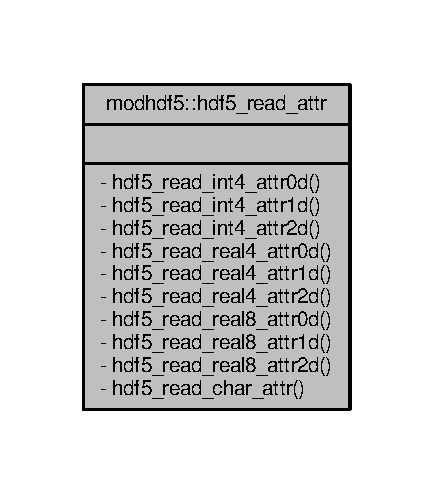
\includegraphics[width=208pt]{interfacemodhdf5_1_1hdf5__read__attr__coll__graph}
\end{center}
\end{figure}
\subsection*{Private Member Functions}
\begin{DoxyCompactItemize}
\item 
subroutine \hyperlink{interfacemodhdf5_1_1hdf5__read__attr_a8f911e83ea7fd98d6198490ba5fed12c}{hdf5\+\_\+read\+\_\+int4\+\_\+attr0d} (id, name, attr)
\begin{DoxyCompactList}\small\item\em Read an integer4 attribute in a hdf5 file. \end{DoxyCompactList}\item 
subroutine \hyperlink{interfacemodhdf5_1_1hdf5__read__attr_afa020293ebd3115b68cbe1fdfa312c4c}{hdf5\+\_\+read\+\_\+int4\+\_\+attr1d} (id, name, n1, attr)
\begin{DoxyCompactList}\small\item\em Read a 1-\/D integer4 attribute in a hdf5 file. \end{DoxyCompactList}\item 
subroutine \hyperlink{interfacemodhdf5_1_1hdf5__read__attr_a455abe5ff52b1fae1e547aebd0c94875}{hdf5\+\_\+read\+\_\+int4\+\_\+attr2d} (id, name, n1, n2, attr)
\begin{DoxyCompactList}\small\item\em Read a 2-\/D integer4 attribute in a hdf5 file. \end{DoxyCompactList}\item 
subroutine \hyperlink{interfacemodhdf5_1_1hdf5__read__attr_ae31cf266133a70be9c4eaa7853b48b19}{hdf5\+\_\+read\+\_\+real4\+\_\+attr0d} (id, name, attr)
\begin{DoxyCompactList}\small\item\em Read a real4 attribute in a hdf5 file. \end{DoxyCompactList}\item 
subroutine \hyperlink{interfacemodhdf5_1_1hdf5__read__attr_abf02aaadb611874adb1b0129be1c0d5c}{hdf5\+\_\+read\+\_\+real4\+\_\+attr1d} (id, name, n1, attr)
\begin{DoxyCompactList}\small\item\em Read a 1-\/D real4 attribute in a hdf5 file. \end{DoxyCompactList}\item 
subroutine \hyperlink{interfacemodhdf5_1_1hdf5__read__attr_a1c6f87720f189a2302ed117e27441c2e}{hdf5\+\_\+read\+\_\+real4\+\_\+attr2d} (id, name, n1, n2, attr)
\begin{DoxyCompactList}\small\item\em Read a 2-\/D real4 attribute in a hdf5 file. \end{DoxyCompactList}\item 
subroutine \hyperlink{interfacemodhdf5_1_1hdf5__read__attr_aa0543551e37cada35de8bc387d679a60}{hdf5\+\_\+read\+\_\+real8\+\_\+attr0d} (id, name, attr)
\begin{DoxyCompactList}\small\item\em Read a real8 attribute in a hdf5 file. \end{DoxyCompactList}\item 
subroutine \hyperlink{interfacemodhdf5_1_1hdf5__read__attr_a00681ffabb305348c87b169a8e541a00}{hdf5\+\_\+read\+\_\+real8\+\_\+attr1d} (id, name, n1, attr)
\begin{DoxyCompactList}\small\item\em Read a 1-\/D real8 attribute in a hdf5 file. \end{DoxyCompactList}\item 
subroutine \hyperlink{interfacemodhdf5_1_1hdf5__read__attr_a81c3ea7a304841609d46f0c39e183fa1}{hdf5\+\_\+read\+\_\+real8\+\_\+attr2d} (id, name, n1, n2, attr)
\begin{DoxyCompactList}\small\item\em Read a 2-\/D real4 attribute in a hdf5 file. \end{DoxyCompactList}\item 
subroutine \hyperlink{interfacemodhdf5_1_1hdf5__read__attr_a12ed53d4b17f713c6dff6d09c93eae93}{hdf5\+\_\+read\+\_\+char\+\_\+attr} (id, name, n1, attr)
\begin{DoxyCompactList}\small\item\em Read string attribute in a hdf5 file. \end{DoxyCompactList}\end{DoxyCompactItemize}


\subsection{Detailed Description}
Generic inteface used to read attributes from a hdf5 file. 


\begin{DoxyParams}[1]{Parameters}
\mbox{\tt in}  & {\em id} & id of the file/group where the attribute will be read \\
\hline
\mbox{\tt in}  & {\em name} & name of the attribute \\
\hline
\mbox{\tt in}  & {\em n1} & first dimension of the attribute array (optional) \\
\hline
\mbox{\tt in}  & {\em n2} & second dimension of the attribute array (optional) \\
\hline
\mbox{\tt in,out}  & {\em data} & 0-\/D, 1-\/D or 2-\/D attribute of type Integer(4), Real(4), Real(8) or Character \\
\hline
\end{DoxyParams}


Definition at line 69 of file modhdf5.\+f90.



\subsection{Member Function/\+Subroutine Documentation}
\index{modhdf5\+::hdf5\+\_\+read\+\_\+attr@{modhdf5\+::hdf5\+\_\+read\+\_\+attr}!hdf5\+\_\+read\+\_\+char\+\_\+attr@{hdf5\+\_\+read\+\_\+char\+\_\+attr}}
\index{hdf5\+\_\+read\+\_\+char\+\_\+attr@{hdf5\+\_\+read\+\_\+char\+\_\+attr}!modhdf5\+::hdf5\+\_\+read\+\_\+attr@{modhdf5\+::hdf5\+\_\+read\+\_\+attr}}
\subsubsection[{\texorpdfstring{hdf5\+\_\+read\+\_\+char\+\_\+attr(id, name, n1, attr)}{hdf5_read_char_attr(id, name, n1, attr)}}]{\setlength{\rightskip}{0pt plus 5cm}subroutine modhdf5\+::hdf5\+\_\+read\+\_\+attr\+::hdf5\+\_\+read\+\_\+char\+\_\+attr (
\begin{DoxyParamCaption}
\item[{integer(kind=hid\+\_\+t), intent(in)}]{id, }
\item[{character(len={\bf h5strlen}), intent(in)}]{name, }
\item[{integer(kind=4), intent(in)}]{n1, }
\item[{character(len=n1), intent(inout)}]{attr}
\end{DoxyParamCaption}
)\hspace{0.3cm}{\ttfamily [private]}}\hypertarget{interfacemodhdf5_1_1hdf5__read__attr_a12ed53d4b17f713c6dff6d09c93eae93}{}\label{interfacemodhdf5_1_1hdf5__read__attr_a12ed53d4b17f713c6dff6d09c93eae93}


Read string attribute in a hdf5 file. 


\begin{DoxyParams}[1]{Parameters}
\mbox{\tt in}  & {\em id} & id of the file/group where the attribute will be read\\
\hline
\mbox{\tt in}  & {\em name} & name of the attribute\\
\hline
\mbox{\tt in}  & {\em n1} & dimension of the attribute string\\
\hline
\mbox{\tt in,out}  & {\em attr} & attribute value \\
\hline
\end{DoxyParams}


Definition at line 3258 of file modhdf5.\+f90.

\index{modhdf5\+::hdf5\+\_\+read\+\_\+attr@{modhdf5\+::hdf5\+\_\+read\+\_\+attr}!hdf5\+\_\+read\+\_\+int4\+\_\+attr0d@{hdf5\+\_\+read\+\_\+int4\+\_\+attr0d}}
\index{hdf5\+\_\+read\+\_\+int4\+\_\+attr0d@{hdf5\+\_\+read\+\_\+int4\+\_\+attr0d}!modhdf5\+::hdf5\+\_\+read\+\_\+attr@{modhdf5\+::hdf5\+\_\+read\+\_\+attr}}
\subsubsection[{\texorpdfstring{hdf5\+\_\+read\+\_\+int4\+\_\+attr0d(id, name, attr)}{hdf5_read_int4_attr0d(id, name, attr)}}]{\setlength{\rightskip}{0pt plus 5cm}subroutine modhdf5\+::hdf5\+\_\+read\+\_\+attr\+::hdf5\+\_\+read\+\_\+int4\+\_\+attr0d (
\begin{DoxyParamCaption}
\item[{integer(kind=hid\+\_\+t), intent(in)}]{id, }
\item[{character(len={\bf h5strlen}), intent(in)}]{name, }
\item[{integer(kind=4), intent(inout)}]{attr}
\end{DoxyParamCaption}
)\hspace{0.3cm}{\ttfamily [private]}}\hypertarget{interfacemodhdf5_1_1hdf5__read__attr_a8f911e83ea7fd98d6198490ba5fed12c}{}\label{interfacemodhdf5_1_1hdf5__read__attr_a8f911e83ea7fd98d6198490ba5fed12c}


Read an integer4 attribute in a hdf5 file. 


\begin{DoxyParams}[1]{Parameters}
\mbox{\tt in}  & {\em id} & id of the file/group where the attribute will be read\\
\hline
\mbox{\tt in}  & {\em name} & name of the attribute\\
\hline
\mbox{\tt in,out}  & {\em attr} & attribute value \\
\hline
\end{DoxyParams}


Definition at line 3026 of file modhdf5.\+f90.

\index{modhdf5\+::hdf5\+\_\+read\+\_\+attr@{modhdf5\+::hdf5\+\_\+read\+\_\+attr}!hdf5\+\_\+read\+\_\+int4\+\_\+attr1d@{hdf5\+\_\+read\+\_\+int4\+\_\+attr1d}}
\index{hdf5\+\_\+read\+\_\+int4\+\_\+attr1d@{hdf5\+\_\+read\+\_\+int4\+\_\+attr1d}!modhdf5\+::hdf5\+\_\+read\+\_\+attr@{modhdf5\+::hdf5\+\_\+read\+\_\+attr}}
\subsubsection[{\texorpdfstring{hdf5\+\_\+read\+\_\+int4\+\_\+attr1d(id, name, n1, attr)}{hdf5_read_int4_attr1d(id, name, n1, attr)}}]{\setlength{\rightskip}{0pt plus 5cm}subroutine modhdf5\+::hdf5\+\_\+read\+\_\+attr\+::hdf5\+\_\+read\+\_\+int4\+\_\+attr1d (
\begin{DoxyParamCaption}
\item[{integer(kind=hid\+\_\+t), intent(in)}]{id, }
\item[{character(len={\bf h5strlen}), intent(in)}]{name, }
\item[{integer(kind=4), intent(in)}]{n1, }
\item[{integer(kind=4), dimension(n1), intent(inout)}]{attr}
\end{DoxyParamCaption}
)\hspace{0.3cm}{\ttfamily [private]}}\hypertarget{interfacemodhdf5_1_1hdf5__read__attr_afa020293ebd3115b68cbe1fdfa312c4c}{}\label{interfacemodhdf5_1_1hdf5__read__attr_afa020293ebd3115b68cbe1fdfa312c4c}


Read a 1-\/D integer4 attribute in a hdf5 file. 


\begin{DoxyParams}[1]{Parameters}
\mbox{\tt in}  & {\em id} & id of the file/group where the attribute will be read\\
\hline
\mbox{\tt in}  & {\em name} & name of the attribute\\
\hline
\mbox{\tt in}  & {\em n1} & dimension of the attribute array\\
\hline
\mbox{\tt in,out}  & {\em attr} & attribute value \\
\hline
\end{DoxyParams}


Definition at line 3054 of file modhdf5.\+f90.

\index{modhdf5\+::hdf5\+\_\+read\+\_\+attr@{modhdf5\+::hdf5\+\_\+read\+\_\+attr}!hdf5\+\_\+read\+\_\+int4\+\_\+attr2d@{hdf5\+\_\+read\+\_\+int4\+\_\+attr2d}}
\index{hdf5\+\_\+read\+\_\+int4\+\_\+attr2d@{hdf5\+\_\+read\+\_\+int4\+\_\+attr2d}!modhdf5\+::hdf5\+\_\+read\+\_\+attr@{modhdf5\+::hdf5\+\_\+read\+\_\+attr}}
\subsubsection[{\texorpdfstring{hdf5\+\_\+read\+\_\+int4\+\_\+attr2d(id, name, n1, n2, attr)}{hdf5_read_int4_attr2d(id, name, n1, n2, attr)}}]{\setlength{\rightskip}{0pt plus 5cm}subroutine modhdf5\+::hdf5\+\_\+read\+\_\+attr\+::hdf5\+\_\+read\+\_\+int4\+\_\+attr2d (
\begin{DoxyParamCaption}
\item[{integer(kind=hid\+\_\+t), intent(in)}]{id, }
\item[{character(len={\bf h5strlen}), intent(in)}]{name, }
\item[{integer(kind=4), intent(in)}]{n1, }
\item[{integer(kind=4), intent(in)}]{n2, }
\item[{integer(kind=4), dimension(n1,n2), intent(inout)}]{attr}
\end{DoxyParamCaption}
)\hspace{0.3cm}{\ttfamily [private]}}\hypertarget{interfacemodhdf5_1_1hdf5__read__attr_a455abe5ff52b1fae1e547aebd0c94875}{}\label{interfacemodhdf5_1_1hdf5__read__attr_a455abe5ff52b1fae1e547aebd0c94875}


Read a 2-\/D integer4 attribute in a hdf5 file. 


\begin{DoxyParams}[1]{Parameters}
\mbox{\tt in}  & {\em id} & id of the file/group where the attribute will be read\\
\hline
\mbox{\tt in}  & {\em name} & name of the attribute\\
\hline
\mbox{\tt in}  & {\em n1} & first dimension of the attribute array\\
\hline
\mbox{\tt in}  & {\em n2} & second dimension of the attribute array\\
\hline
\mbox{\tt in,out}  & {\em attr} & attribute value \\
\hline
\end{DoxyParams}


Definition at line 3079 of file modhdf5.\+f90.

\index{modhdf5\+::hdf5\+\_\+read\+\_\+attr@{modhdf5\+::hdf5\+\_\+read\+\_\+attr}!hdf5\+\_\+read\+\_\+real4\+\_\+attr0d@{hdf5\+\_\+read\+\_\+real4\+\_\+attr0d}}
\index{hdf5\+\_\+read\+\_\+real4\+\_\+attr0d@{hdf5\+\_\+read\+\_\+real4\+\_\+attr0d}!modhdf5\+::hdf5\+\_\+read\+\_\+attr@{modhdf5\+::hdf5\+\_\+read\+\_\+attr}}
\subsubsection[{\texorpdfstring{hdf5\+\_\+read\+\_\+real4\+\_\+attr0d(id, name, attr)}{hdf5_read_real4_attr0d(id, name, attr)}}]{\setlength{\rightskip}{0pt plus 5cm}subroutine modhdf5\+::hdf5\+\_\+read\+\_\+attr\+::hdf5\+\_\+read\+\_\+real4\+\_\+attr0d (
\begin{DoxyParamCaption}
\item[{integer(kind=hid\+\_\+t), intent(in)}]{id, }
\item[{character(len={\bf h5strlen}), intent(in)}]{name, }
\item[{real(kind=4), intent(inout)}]{attr}
\end{DoxyParamCaption}
)\hspace{0.3cm}{\ttfamily [private]}}\hypertarget{interfacemodhdf5_1_1hdf5__read__attr_ae31cf266133a70be9c4eaa7853b48b19}{}\label{interfacemodhdf5_1_1hdf5__read__attr_ae31cf266133a70be9c4eaa7853b48b19}


Read a real4 attribute in a hdf5 file. 


\begin{DoxyParams}[1]{Parameters}
\mbox{\tt in}  & {\em id} & id of the file/group where the attribute will be read\\
\hline
\mbox{\tt in}  & {\em name} & name of the attribute\\
\hline
\mbox{\tt in,out}  & {\em attr} & attribute value \\
\hline
\end{DoxyParams}


Definition at line 3106 of file modhdf5.\+f90.

\index{modhdf5\+::hdf5\+\_\+read\+\_\+attr@{modhdf5\+::hdf5\+\_\+read\+\_\+attr}!hdf5\+\_\+read\+\_\+real4\+\_\+attr1d@{hdf5\+\_\+read\+\_\+real4\+\_\+attr1d}}
\index{hdf5\+\_\+read\+\_\+real4\+\_\+attr1d@{hdf5\+\_\+read\+\_\+real4\+\_\+attr1d}!modhdf5\+::hdf5\+\_\+read\+\_\+attr@{modhdf5\+::hdf5\+\_\+read\+\_\+attr}}
\subsubsection[{\texorpdfstring{hdf5\+\_\+read\+\_\+real4\+\_\+attr1d(id, name, n1, attr)}{hdf5_read_real4_attr1d(id, name, n1, attr)}}]{\setlength{\rightskip}{0pt plus 5cm}subroutine modhdf5\+::hdf5\+\_\+read\+\_\+attr\+::hdf5\+\_\+read\+\_\+real4\+\_\+attr1d (
\begin{DoxyParamCaption}
\item[{integer(kind=hid\+\_\+t), intent(in)}]{id, }
\item[{character(len={\bf h5strlen}), intent(in)}]{name, }
\item[{integer(kind=4), intent(in)}]{n1, }
\item[{real(kind=4), dimension(n1), intent(inout)}]{attr}
\end{DoxyParamCaption}
)\hspace{0.3cm}{\ttfamily [private]}}\hypertarget{interfacemodhdf5_1_1hdf5__read__attr_abf02aaadb611874adb1b0129be1c0d5c}{}\label{interfacemodhdf5_1_1hdf5__read__attr_abf02aaadb611874adb1b0129be1c0d5c}


Read a 1-\/D real4 attribute in a hdf5 file. 


\begin{DoxyParams}[1]{Parameters}
\mbox{\tt in}  & {\em id} & id of the file/group where the attribute will be read\\
\hline
\mbox{\tt in}  & {\em name} & name of the attribute\\
\hline
\mbox{\tt in}  & {\em n1} & dimension of the attribute array\\
\hline
\mbox{\tt in,out}  & {\em attr} & attribute value \\
\hline
\end{DoxyParams}


Definition at line 3130 of file modhdf5.\+f90.

\index{modhdf5\+::hdf5\+\_\+read\+\_\+attr@{modhdf5\+::hdf5\+\_\+read\+\_\+attr}!hdf5\+\_\+read\+\_\+real4\+\_\+attr2d@{hdf5\+\_\+read\+\_\+real4\+\_\+attr2d}}
\index{hdf5\+\_\+read\+\_\+real4\+\_\+attr2d@{hdf5\+\_\+read\+\_\+real4\+\_\+attr2d}!modhdf5\+::hdf5\+\_\+read\+\_\+attr@{modhdf5\+::hdf5\+\_\+read\+\_\+attr}}
\subsubsection[{\texorpdfstring{hdf5\+\_\+read\+\_\+real4\+\_\+attr2d(id, name, n1, n2, attr)}{hdf5_read_real4_attr2d(id, name, n1, n2, attr)}}]{\setlength{\rightskip}{0pt plus 5cm}subroutine modhdf5\+::hdf5\+\_\+read\+\_\+attr\+::hdf5\+\_\+read\+\_\+real4\+\_\+attr2d (
\begin{DoxyParamCaption}
\item[{integer(kind=hid\+\_\+t), intent(in)}]{id, }
\item[{character(len={\bf h5strlen}), intent(in)}]{name, }
\item[{integer(kind=4), intent(in)}]{n1, }
\item[{integer(kind=4), intent(in)}]{n2, }
\item[{real(kind=4), dimension(n1,n2), intent(inout)}]{attr}
\end{DoxyParamCaption}
)\hspace{0.3cm}{\ttfamily [private]}}\hypertarget{interfacemodhdf5_1_1hdf5__read__attr_a1c6f87720f189a2302ed117e27441c2e}{}\label{interfacemodhdf5_1_1hdf5__read__attr_a1c6f87720f189a2302ed117e27441c2e}


Read a 2-\/D real4 attribute in a hdf5 file. 


\begin{DoxyParams}[1]{Parameters}
\mbox{\tt in}  & {\em id} & id of the file/group where the attribute will be read\\
\hline
\mbox{\tt in}  & {\em name} & name of the attribute\\
\hline
\mbox{\tt in}  & {\em n1} & first dimension of the attribute array\\
\hline
\mbox{\tt in}  & {\em n2} & second dimension of the attribute array\\
\hline
\mbox{\tt in,out}  & {\em attr} & attribute value \\
\hline
\end{DoxyParams}


Definition at line 3155 of file modhdf5.\+f90.

\index{modhdf5\+::hdf5\+\_\+read\+\_\+attr@{modhdf5\+::hdf5\+\_\+read\+\_\+attr}!hdf5\+\_\+read\+\_\+real8\+\_\+attr0d@{hdf5\+\_\+read\+\_\+real8\+\_\+attr0d}}
\index{hdf5\+\_\+read\+\_\+real8\+\_\+attr0d@{hdf5\+\_\+read\+\_\+real8\+\_\+attr0d}!modhdf5\+::hdf5\+\_\+read\+\_\+attr@{modhdf5\+::hdf5\+\_\+read\+\_\+attr}}
\subsubsection[{\texorpdfstring{hdf5\+\_\+read\+\_\+real8\+\_\+attr0d(id, name, attr)}{hdf5_read_real8_attr0d(id, name, attr)}}]{\setlength{\rightskip}{0pt plus 5cm}subroutine modhdf5\+::hdf5\+\_\+read\+\_\+attr\+::hdf5\+\_\+read\+\_\+real8\+\_\+attr0d (
\begin{DoxyParamCaption}
\item[{integer(kind=hid\+\_\+t), intent(in)}]{id, }
\item[{character(len={\bf h5strlen}), intent(in)}]{name, }
\item[{real(kind=8), intent(inout)}]{attr}
\end{DoxyParamCaption}
)\hspace{0.3cm}{\ttfamily [private]}}\hypertarget{interfacemodhdf5_1_1hdf5__read__attr_aa0543551e37cada35de8bc387d679a60}{}\label{interfacemodhdf5_1_1hdf5__read__attr_aa0543551e37cada35de8bc387d679a60}


Read a real8 attribute in a hdf5 file. 


\begin{DoxyParams}[1]{Parameters}
\mbox{\tt in}  & {\em id} & id of the file/group where the attribute will be read\\
\hline
\mbox{\tt in}  & {\em name} & name of the attribute\\
\hline
\mbox{\tt in,out}  & {\em attr} & attribute value \\
\hline
\end{DoxyParams}


Definition at line 3182 of file modhdf5.\+f90.

\index{modhdf5\+::hdf5\+\_\+read\+\_\+attr@{modhdf5\+::hdf5\+\_\+read\+\_\+attr}!hdf5\+\_\+read\+\_\+real8\+\_\+attr1d@{hdf5\+\_\+read\+\_\+real8\+\_\+attr1d}}
\index{hdf5\+\_\+read\+\_\+real8\+\_\+attr1d@{hdf5\+\_\+read\+\_\+real8\+\_\+attr1d}!modhdf5\+::hdf5\+\_\+read\+\_\+attr@{modhdf5\+::hdf5\+\_\+read\+\_\+attr}}
\subsubsection[{\texorpdfstring{hdf5\+\_\+read\+\_\+real8\+\_\+attr1d(id, name, n1, attr)}{hdf5_read_real8_attr1d(id, name, n1, attr)}}]{\setlength{\rightskip}{0pt plus 5cm}subroutine modhdf5\+::hdf5\+\_\+read\+\_\+attr\+::hdf5\+\_\+read\+\_\+real8\+\_\+attr1d (
\begin{DoxyParamCaption}
\item[{integer(kind=hid\+\_\+t), intent(in)}]{id, }
\item[{character(len={\bf h5strlen}), intent(in)}]{name, }
\item[{integer(kind=4), intent(in)}]{n1, }
\item[{real(kind=8), dimension(n1), intent(inout)}]{attr}
\end{DoxyParamCaption}
)\hspace{0.3cm}{\ttfamily [private]}}\hypertarget{interfacemodhdf5_1_1hdf5__read__attr_a00681ffabb305348c87b169a8e541a00}{}\label{interfacemodhdf5_1_1hdf5__read__attr_a00681ffabb305348c87b169a8e541a00}


Read a 1-\/D real8 attribute in a hdf5 file. 


\begin{DoxyParams}[1]{Parameters}
\mbox{\tt in}  & {\em id} & id of the file/group where the attribute will be read\\
\hline
\mbox{\tt in}  & {\em name} & name of the attribute\\
\hline
\mbox{\tt in}  & {\em n1} & dimension of the attribute array\\
\hline
\mbox{\tt in,out}  & {\em attr} & attribute value \\
\hline
\end{DoxyParams}


Definition at line 3206 of file modhdf5.\+f90.

\index{modhdf5\+::hdf5\+\_\+read\+\_\+attr@{modhdf5\+::hdf5\+\_\+read\+\_\+attr}!hdf5\+\_\+read\+\_\+real8\+\_\+attr2d@{hdf5\+\_\+read\+\_\+real8\+\_\+attr2d}}
\index{hdf5\+\_\+read\+\_\+real8\+\_\+attr2d@{hdf5\+\_\+read\+\_\+real8\+\_\+attr2d}!modhdf5\+::hdf5\+\_\+read\+\_\+attr@{modhdf5\+::hdf5\+\_\+read\+\_\+attr}}
\subsubsection[{\texorpdfstring{hdf5\+\_\+read\+\_\+real8\+\_\+attr2d(id, name, n1, n2, attr)}{hdf5_read_real8_attr2d(id, name, n1, n2, attr)}}]{\setlength{\rightskip}{0pt plus 5cm}subroutine modhdf5\+::hdf5\+\_\+read\+\_\+attr\+::hdf5\+\_\+read\+\_\+real8\+\_\+attr2d (
\begin{DoxyParamCaption}
\item[{integer(kind=hid\+\_\+t), intent(in)}]{id, }
\item[{character(len={\bf h5strlen}), intent(in)}]{name, }
\item[{integer(kind=4), intent(in)}]{n1, }
\item[{integer(kind=4), intent(in)}]{n2, }
\item[{real(kind=8), dimension(n1,n2), intent(inout)}]{attr}
\end{DoxyParamCaption}
)\hspace{0.3cm}{\ttfamily [private]}}\hypertarget{interfacemodhdf5_1_1hdf5__read__attr_a81c3ea7a304841609d46f0c39e183fa1}{}\label{interfacemodhdf5_1_1hdf5__read__attr_a81c3ea7a304841609d46f0c39e183fa1}


Read a 2-\/D real4 attribute in a hdf5 file. 


\begin{DoxyParams}[1]{Parameters}
\mbox{\tt in}  & {\em id} & id of the file/group where the attribute will be read\\
\hline
\mbox{\tt in}  & {\em name} & name of the attribute\\
\hline
\mbox{\tt in}  & {\em n1} & first dimension of the attribute array\\
\hline
\mbox{\tt in}  & {\em n2} & second dimension of the attribute array\\
\hline
\mbox{\tt in,out}  & {\em attr} & attribute value \\
\hline
\end{DoxyParams}


Definition at line 3231 of file modhdf5.\+f90.



The documentation for this interface was generated from the following file\+:\begin{DoxyCompactItemize}
\item 
/home/roy/\+Travail/\+Devel/\+Cosmologie/\+Pfof/trunk/common/src/\hyperlink{modhdf5_8f90}{modhdf5.\+f90}\end{DoxyCompactItemize}

\hypertarget{interfacemodhdf5_1_1hdf5__read__data}{\section{modhdf5\-:\-:hdf5\-\_\-read\-\_\-data Interface Reference}
\label{interfacemodhdf5_1_1hdf5__read__data}\index{modhdf5\-::hdf5\-\_\-read\-\_\-data@{modhdf5\-::hdf5\-\_\-read\-\_\-data}}
}


Generic inteface used to read data from a hdf5 file.  


\subsection*{Private Member Functions}
\begin{DoxyCompactItemize}
\item 
subroutine \hyperlink{interfacemodhdf5_1_1hdf5__read__data_a484bfd3272dfc507ab6f7ee71bd60232}{hdf5\-\_\-read\-\_\-int4\-\_\-1d} (id, name, n1, data)
\begin{DoxyCompactList}\small\item\em Read a 1-\/\-D integer(kind=4) array from a serial file. \end{DoxyCompactList}\item 
subroutine \hyperlink{interfacemodhdf5_1_1hdf5__read__data_aebc8b06d547dd0b0a64e8d76bf9b933e}{hdf5\-\_\-read\-\_\-int4\-\_\-2d} (id, name, n1, n2, data)
\begin{DoxyCompactList}\small\item\em Read a 2-\/\-D integer(kind=4) array from a serial file. \end{DoxyCompactList}\item 
subroutine \hyperlink{interfacemodhdf5_1_1hdf5__read__data_a4b43a721044be9ae8155dcff0dc54753}{hdf5\-\_\-read\-\_\-int8\-\_\-0d} (id, name, data)
\begin{DoxyCompactList}\small\item\em Read a 1-\/\-D integer(kind=8) scalar from a serial file. \end{DoxyCompactList}\item 
subroutine \hyperlink{interfacemodhdf5_1_1hdf5__read__data_ae4d30f084b576d04638ddc6c8d35a490}{hdf5\-\_\-read\-\_\-int8\-\_\-1d} (id, name, n1, data)
\begin{DoxyCompactList}\small\item\em Read a 1-\/\-D integer(kind=8) array from a serial file. \end{DoxyCompactList}\item 
subroutine \hyperlink{interfacemodhdf5_1_1hdf5__read__data_aac8b36f082332a365fc9f89d1f7df37a}{hdf5\-\_\-read\-\_\-int8\-\_\-2d} (id, name, n1, n2, data)
\begin{DoxyCompactList}\small\item\em Read a 2-\/\-D integer(kind=8) array from a serial file. \end{DoxyCompactList}\item 
subroutine \hyperlink{interfacemodhdf5_1_1hdf5__read__data_a8ffa6d8d59ce7a75ff6f2e36ebacc154}{hdf5\-\_\-read\-\_\-real4\-\_\-1d} (id, name, n1, data)
\begin{DoxyCompactList}\small\item\em Read a 1-\/\-D real(kind=4) array from a serial file. \end{DoxyCompactList}\item 
subroutine \hyperlink{interfacemodhdf5_1_1hdf5__read__data_a3777ea5fe47dbc804b4222a9cf4b7764}{hdf5\-\_\-read\-\_\-real4\-\_\-2d} (id, name, n1, n2, data)
\begin{DoxyCompactList}\small\item\em Read a 2-\/\-D real(kind=4) array from a serial file. \end{DoxyCompactList}\item 
subroutine \hyperlink{interfacemodhdf5_1_1hdf5__read__data_aa973c89b98368b9db76914684391b033}{hdf5\-\_\-read\-\_\-real8\-\_\-1d} (id, name, n1, data)
\begin{DoxyCompactList}\small\item\em Read a 1-\/\-D real(kind=8) array from a serial file. \end{DoxyCompactList}\item 
subroutine \hyperlink{interfacemodhdf5_1_1hdf5__read__data_a498e25c3377710f2d13c14e587df327d}{hdf5\-\_\-read\-\_\-real8\-\_\-2d} (id, name, n1, n2, data)
\begin{DoxyCompactList}\small\item\em Read a 2-\/\-D real(kind=8) array from a serial file. \end{DoxyCompactList}\end{DoxyCompactItemize}


\subsection{Detailed Description}
Generic inteface used to read data from a hdf5 file. 


\begin{DoxyParams}[1]{Parameters}
\mbox{\tt in}  & {\em id} & id of the file/group where the dataset will be read \\
\hline
\mbox{\tt in}  & {\em name} & name of the dataset \\
\hline
\mbox{\tt in}  & {\em n1} & first dimension of the data array \\
\hline
\mbox{\tt in}  & {\em n2} & second dimension of the data array (optional) \\
\hline
\mbox{\tt in,out}  & {\em data} & 1-\/\-D or 2-\/\-D data array of type Integer(4), Integer(8), Real(4) or Real(8) \\
\hline
\end{DoxyParams}


Definition at line 106 of file modhdf5.\-f90.



\subsection{Member Function/\-Subroutine Documentation}
\hypertarget{interfacemodhdf5_1_1hdf5__read__data_a484bfd3272dfc507ab6f7ee71bd60232}{\index{modhdf5\-::hdf5\-\_\-read\-\_\-data@{modhdf5\-::hdf5\-\_\-read\-\_\-data}!hdf5\-\_\-read\-\_\-int4\-\_\-1d@{hdf5\-\_\-read\-\_\-int4\-\_\-1d}}
\index{hdf5\-\_\-read\-\_\-int4\-\_\-1d@{hdf5\-\_\-read\-\_\-int4\-\_\-1d}!modhdf5::hdf5_read_data@{modhdf5\-::hdf5\-\_\-read\-\_\-data}}
\subsubsection[{hdf5\-\_\-read\-\_\-int4\-\_\-1d}]{\setlength{\rightskip}{0pt plus 5cm}subroutine modhdf5\-::hdf5\-\_\-read\-\_\-data\-::hdf5\-\_\-read\-\_\-int4\-\_\-1d (
\begin{DoxyParamCaption}
\item[{integer(hid\-\_\-t), intent(in)}]{id, }
\item[{character(len={\bf h5strlen}), intent(in)}]{name, }
\item[{integer(kind=4), intent(in)}]{n1, }
\item[{integer(kind=4), dimension(n1), intent(inout), target}]{data}
\end{DoxyParamCaption}
)\hspace{0.3cm}{\ttfamily [private]}}}\label{interfacemodhdf5_1_1hdf5__read__data_a484bfd3272dfc507ab6f7ee71bd60232}


Read a 1-\/\-D integer(kind=4) array from a serial file. 


\begin{DoxyParams}[1]{Parameters}
\mbox{\tt in}  & {\em id} & id of the file/group where the dataset will be read\\
\hline
\mbox{\tt in}  & {\em name} & name of the dataset\\
\hline
\mbox{\tt in}  & {\em n1} & dimension of the array to read\\
\hline
\mbox{\tt in,out}  & {\em data} & array \\
\hline
\end{DoxyParams}


Definition at line 1731 of file modhdf5.\-f90.

\hypertarget{interfacemodhdf5_1_1hdf5__read__data_aebc8b06d547dd0b0a64e8d76bf9b933e}{\index{modhdf5\-::hdf5\-\_\-read\-\_\-data@{modhdf5\-::hdf5\-\_\-read\-\_\-data}!hdf5\-\_\-read\-\_\-int4\-\_\-2d@{hdf5\-\_\-read\-\_\-int4\-\_\-2d}}
\index{hdf5\-\_\-read\-\_\-int4\-\_\-2d@{hdf5\-\_\-read\-\_\-int4\-\_\-2d}!modhdf5::hdf5_read_data@{modhdf5\-::hdf5\-\_\-read\-\_\-data}}
\subsubsection[{hdf5\-\_\-read\-\_\-int4\-\_\-2d}]{\setlength{\rightskip}{0pt plus 5cm}subroutine modhdf5\-::hdf5\-\_\-read\-\_\-data\-::hdf5\-\_\-read\-\_\-int4\-\_\-2d (
\begin{DoxyParamCaption}
\item[{integer(hid\-\_\-t), intent(in)}]{id, }
\item[{character(len={\bf h5strlen}), intent(in)}]{name, }
\item[{integer(kind=4), intent(in)}]{n1, }
\item[{integer(kind=4), intent(in)}]{n2, }
\item[{integer(kind=4), dimension(n1,n2), intent(inout), target}]{data}
\end{DoxyParamCaption}
)\hspace{0.3cm}{\ttfamily [private]}}}\label{interfacemodhdf5_1_1hdf5__read__data_aebc8b06d547dd0b0a64e8d76bf9b933e}


Read a 2-\/\-D integer(kind=4) array from a serial file. 


\begin{DoxyParams}[1]{Parameters}
\mbox{\tt in}  & {\em id} & id of the file/group where the dataset will be read\\
\hline
\mbox{\tt in}  & {\em name} & name of the dataset\\
\hline
\mbox{\tt in}  & {\em n1} & first dimension of the array to read\\
\hline
\mbox{\tt in}  & {\em n2} & second dimension of the array to read\\
\hline
\mbox{\tt in,out}  & {\em data} & array \\
\hline
\end{DoxyParams}


Definition at line 1838 of file modhdf5.\-f90.

\hypertarget{interfacemodhdf5_1_1hdf5__read__data_a4b43a721044be9ae8155dcff0dc54753}{\index{modhdf5\-::hdf5\-\_\-read\-\_\-data@{modhdf5\-::hdf5\-\_\-read\-\_\-data}!hdf5\-\_\-read\-\_\-int8\-\_\-0d@{hdf5\-\_\-read\-\_\-int8\-\_\-0d}}
\index{hdf5\-\_\-read\-\_\-int8\-\_\-0d@{hdf5\-\_\-read\-\_\-int8\-\_\-0d}!modhdf5::hdf5_read_data@{modhdf5\-::hdf5\-\_\-read\-\_\-data}}
\subsubsection[{hdf5\-\_\-read\-\_\-int8\-\_\-0d}]{\setlength{\rightskip}{0pt plus 5cm}subroutine modhdf5\-::hdf5\-\_\-read\-\_\-data\-::hdf5\-\_\-read\-\_\-int8\-\_\-0d (
\begin{DoxyParamCaption}
\item[{integer(hid\-\_\-t), intent(in)}]{id, }
\item[{character(len={\bf h5strlen}), intent(in)}]{name, }
\item[{integer(kind=8), intent(inout), target}]{data}
\end{DoxyParamCaption}
)\hspace{0.3cm}{\ttfamily [private]}}}\label{interfacemodhdf5_1_1hdf5__read__data_a4b43a721044be9ae8155dcff0dc54753}


Read a 1-\/\-D integer(kind=8) scalar from a serial file. 


\begin{DoxyParams}[1]{Parameters}
\mbox{\tt in}  & {\em id} & id of the file/group where the dataset will be read\\
\hline
\mbox{\tt in}  & {\em name} & name of the dataset\\
\hline
\mbox{\tt in,out}  & {\em data} & array \\
\hline
\end{DoxyParams}


Definition at line 1777 of file modhdf5.\-f90.

\hypertarget{interfacemodhdf5_1_1hdf5__read__data_ae4d30f084b576d04638ddc6c8d35a490}{\index{modhdf5\-::hdf5\-\_\-read\-\_\-data@{modhdf5\-::hdf5\-\_\-read\-\_\-data}!hdf5\-\_\-read\-\_\-int8\-\_\-1d@{hdf5\-\_\-read\-\_\-int8\-\_\-1d}}
\index{hdf5\-\_\-read\-\_\-int8\-\_\-1d@{hdf5\-\_\-read\-\_\-int8\-\_\-1d}!modhdf5::hdf5_read_data@{modhdf5\-::hdf5\-\_\-read\-\_\-data}}
\subsubsection[{hdf5\-\_\-read\-\_\-int8\-\_\-1d}]{\setlength{\rightskip}{0pt plus 5cm}subroutine modhdf5\-::hdf5\-\_\-read\-\_\-data\-::hdf5\-\_\-read\-\_\-int8\-\_\-1d (
\begin{DoxyParamCaption}
\item[{integer(hid\-\_\-t), intent(in)}]{id, }
\item[{character(len={\bf h5strlen}), intent(in)}]{name, }
\item[{integer(kind=4), intent(in)}]{n1, }
\item[{integer(kind=8), dimension(n1), intent(inout), target}]{data}
\end{DoxyParamCaption}
)\hspace{0.3cm}{\ttfamily [private]}}}\label{interfacemodhdf5_1_1hdf5__read__data_ae4d30f084b576d04638ddc6c8d35a490}


Read a 1-\/\-D integer(kind=8) array from a serial file. 


\begin{DoxyParams}[1]{Parameters}
\mbox{\tt in}  & {\em id} & id of the file/group where the dataset will be read\\
\hline
\mbox{\tt in}  & {\em name} & name of the dataset\\
\hline
\mbox{\tt in}  & {\em n1} & dimension of the array to read\\
\hline
\mbox{\tt in,out}  & {\em data} & array \\
\hline
\end{DoxyParams}


Definition at line 1807 of file modhdf5.\-f90.

\hypertarget{interfacemodhdf5_1_1hdf5__read__data_aac8b36f082332a365fc9f89d1f7df37a}{\index{modhdf5\-::hdf5\-\_\-read\-\_\-data@{modhdf5\-::hdf5\-\_\-read\-\_\-data}!hdf5\-\_\-read\-\_\-int8\-\_\-2d@{hdf5\-\_\-read\-\_\-int8\-\_\-2d}}
\index{hdf5\-\_\-read\-\_\-int8\-\_\-2d@{hdf5\-\_\-read\-\_\-int8\-\_\-2d}!modhdf5::hdf5_read_data@{modhdf5\-::hdf5\-\_\-read\-\_\-data}}
\subsubsection[{hdf5\-\_\-read\-\_\-int8\-\_\-2d}]{\setlength{\rightskip}{0pt plus 5cm}subroutine modhdf5\-::hdf5\-\_\-read\-\_\-data\-::hdf5\-\_\-read\-\_\-int8\-\_\-2d (
\begin{DoxyParamCaption}
\item[{integer(hid\-\_\-t), intent(in)}]{id, }
\item[{character(len={\bf h5strlen}), intent(in)}]{name, }
\item[{integer(kind=4), intent(in)}]{n1, }
\item[{integer(kind=4), intent(in)}]{n2, }
\item[{integer(kind=8), dimension(n1,n2), intent(inout), target}]{data}
\end{DoxyParamCaption}
)\hspace{0.3cm}{\ttfamily [private]}}}\label{interfacemodhdf5_1_1hdf5__read__data_aac8b36f082332a365fc9f89d1f7df37a}


Read a 2-\/\-D integer(kind=8) array from a serial file. 


\begin{DoxyParams}[1]{Parameters}
\mbox{\tt in}  & {\em id} & id of the file/group where the dataset will be read\\
\hline
\mbox{\tt in}  & {\em name} & name of the dataset\\
\hline
\mbox{\tt in}  & {\em n1} & first dimension of the array to read\\
\hline
\mbox{\tt in}  & {\em n2} & second dimension of the array to read\\
\hline
\mbox{\tt in,out}  & {\em data} & array \\
\hline
\end{DoxyParams}


Definition at line 1870 of file modhdf5.\-f90.

\hypertarget{interfacemodhdf5_1_1hdf5__read__data_a8ffa6d8d59ce7a75ff6f2e36ebacc154}{\index{modhdf5\-::hdf5\-\_\-read\-\_\-data@{modhdf5\-::hdf5\-\_\-read\-\_\-data}!hdf5\-\_\-read\-\_\-real4\-\_\-1d@{hdf5\-\_\-read\-\_\-real4\-\_\-1d}}
\index{hdf5\-\_\-read\-\_\-real4\-\_\-1d@{hdf5\-\_\-read\-\_\-real4\-\_\-1d}!modhdf5::hdf5_read_data@{modhdf5\-::hdf5\-\_\-read\-\_\-data}}
\subsubsection[{hdf5\-\_\-read\-\_\-real4\-\_\-1d}]{\setlength{\rightskip}{0pt plus 5cm}subroutine modhdf5\-::hdf5\-\_\-read\-\_\-data\-::hdf5\-\_\-read\-\_\-real4\-\_\-1d (
\begin{DoxyParamCaption}
\item[{integer(hid\-\_\-t), intent(in)}]{id, }
\item[{character(len={\bf h5strlen}), intent(in)}]{name, }
\item[{integer(kind=4), intent(in)}]{n1, }
\item[{real(kind=4), dimension(n1), intent(inout), target}]{data}
\end{DoxyParamCaption}
)\hspace{0.3cm}{\ttfamily [private]}}}\label{interfacemodhdf5_1_1hdf5__read__data_a8ffa6d8d59ce7a75ff6f2e36ebacc154}


Read a 1-\/\-D real(kind=4) array from a serial file. 


\begin{DoxyParams}[1]{Parameters}
\mbox{\tt in}  & {\em id} & id of the file/group where the dataset will be read\\
\hline
\mbox{\tt in}  & {\em name} & name of the dataset\\
\hline
\mbox{\tt in}  & {\em n1} & dimension of the array to read\\
\hline
\mbox{\tt in,out}  & {\em data} & array \\
\hline
\end{DoxyParams}


Definition at line 1902 of file modhdf5.\-f90.

\hypertarget{interfacemodhdf5_1_1hdf5__read__data_a3777ea5fe47dbc804b4222a9cf4b7764}{\index{modhdf5\-::hdf5\-\_\-read\-\_\-data@{modhdf5\-::hdf5\-\_\-read\-\_\-data}!hdf5\-\_\-read\-\_\-real4\-\_\-2d@{hdf5\-\_\-read\-\_\-real4\-\_\-2d}}
\index{hdf5\-\_\-read\-\_\-real4\-\_\-2d@{hdf5\-\_\-read\-\_\-real4\-\_\-2d}!modhdf5::hdf5_read_data@{modhdf5\-::hdf5\-\_\-read\-\_\-data}}
\subsubsection[{hdf5\-\_\-read\-\_\-real4\-\_\-2d}]{\setlength{\rightskip}{0pt plus 5cm}subroutine modhdf5\-::hdf5\-\_\-read\-\_\-data\-::hdf5\-\_\-read\-\_\-real4\-\_\-2d (
\begin{DoxyParamCaption}
\item[{integer(hid\-\_\-t), intent(in)}]{id, }
\item[{character(len={\bf h5strlen}), intent(in)}]{name, }
\item[{integer(kind=4), intent(in)}]{n1, }
\item[{integer(kind=4), intent(in)}]{n2, }
\item[{real(kind=4), dimension(n1,n2), intent(inout), target}]{data}
\end{DoxyParamCaption}
)\hspace{0.3cm}{\ttfamily [private]}}}\label{interfacemodhdf5_1_1hdf5__read__data_a3777ea5fe47dbc804b4222a9cf4b7764}


Read a 2-\/\-D real(kind=4) array from a serial file. 


\begin{DoxyParams}[1]{Parameters}
\mbox{\tt in}  & {\em id} & id of the file/group where the dataset will be read\\
\hline
\mbox{\tt in}  & {\em name} & name of the dataset\\
\hline
\mbox{\tt in}  & {\em n1} & first dimension of the array to read\\
\hline
\mbox{\tt in}  & {\em n2} & second dimension of the array to read\\
\hline
\mbox{\tt in,out}  & {\em data} & array \\
\hline
\end{DoxyParams}


Definition at line 1964 of file modhdf5.\-f90.

\hypertarget{interfacemodhdf5_1_1hdf5__read__data_aa973c89b98368b9db76914684391b033}{\index{modhdf5\-::hdf5\-\_\-read\-\_\-data@{modhdf5\-::hdf5\-\_\-read\-\_\-data}!hdf5\-\_\-read\-\_\-real8\-\_\-1d@{hdf5\-\_\-read\-\_\-real8\-\_\-1d}}
\index{hdf5\-\_\-read\-\_\-real8\-\_\-1d@{hdf5\-\_\-read\-\_\-real8\-\_\-1d}!modhdf5::hdf5_read_data@{modhdf5\-::hdf5\-\_\-read\-\_\-data}}
\subsubsection[{hdf5\-\_\-read\-\_\-real8\-\_\-1d}]{\setlength{\rightskip}{0pt plus 5cm}subroutine modhdf5\-::hdf5\-\_\-read\-\_\-data\-::hdf5\-\_\-read\-\_\-real8\-\_\-1d (
\begin{DoxyParamCaption}
\item[{integer(hid\-\_\-t), intent(in)}]{id, }
\item[{character(len={\bf h5strlen}), intent(in)}]{name, }
\item[{integer(kind=4), intent(in)}]{n1, }
\item[{real(kind=8), dimension(n1), intent(inout), target}]{data}
\end{DoxyParamCaption}
)\hspace{0.3cm}{\ttfamily [private]}}}\label{interfacemodhdf5_1_1hdf5__read__data_aa973c89b98368b9db76914684391b033}


Read a 1-\/\-D real(kind=8) array from a serial file. 


\begin{DoxyParams}[1]{Parameters}
\mbox{\tt in}  & {\em id} & id of the file/group where the dataset will be read\\
\hline
\mbox{\tt in}  & {\em name} & name of the dataset\\
\hline
\mbox{\tt in}  & {\em n1} & dimension of the array to read\\
\hline
\mbox{\tt in,out}  & {\em data} & array \\
\hline
\end{DoxyParams}


Definition at line 1933 of file modhdf5.\-f90.

\hypertarget{interfacemodhdf5_1_1hdf5__read__data_a498e25c3377710f2d13c14e587df327d}{\index{modhdf5\-::hdf5\-\_\-read\-\_\-data@{modhdf5\-::hdf5\-\_\-read\-\_\-data}!hdf5\-\_\-read\-\_\-real8\-\_\-2d@{hdf5\-\_\-read\-\_\-real8\-\_\-2d}}
\index{hdf5\-\_\-read\-\_\-real8\-\_\-2d@{hdf5\-\_\-read\-\_\-real8\-\_\-2d}!modhdf5::hdf5_read_data@{modhdf5\-::hdf5\-\_\-read\-\_\-data}}
\subsubsection[{hdf5\-\_\-read\-\_\-real8\-\_\-2d}]{\setlength{\rightskip}{0pt plus 5cm}subroutine modhdf5\-::hdf5\-\_\-read\-\_\-data\-::hdf5\-\_\-read\-\_\-real8\-\_\-2d (
\begin{DoxyParamCaption}
\item[{integer(hid\-\_\-t), intent(in)}]{id, }
\item[{character(len={\bf h5strlen}), intent(in)}]{name, }
\item[{integer(kind=4), intent(in)}]{n1, }
\item[{integer(kind=4), intent(in)}]{n2, }
\item[{real(kind=8), dimension(n1,n2), intent(inout), target}]{data}
\end{DoxyParamCaption}
)\hspace{0.3cm}{\ttfamily [private]}}}\label{interfacemodhdf5_1_1hdf5__read__data_a498e25c3377710f2d13c14e587df327d}


Read a 2-\/\-D real(kind=8) array from a serial file. 


\begin{DoxyParams}[1]{Parameters}
\mbox{\tt in}  & {\em id} & id of the file/group where the dataset will be read\\
\hline
\mbox{\tt in}  & {\em name} & name of the dataset\\
\hline
\mbox{\tt in}  & {\em n1} & first dimension of the array to read\\
\hline
\mbox{\tt in}  & {\em n2} & second dimension of the array to read\\
\hline
\mbox{\tt in,out}  & {\em data} & array \\
\hline
\end{DoxyParams}


Definition at line 1996 of file modhdf5.\-f90.



The documentation for this interface was generated from the following file\-:\begin{DoxyCompactItemize}
\item 
/home/roy/\-Travail/\-Devel/\-Cosmologie/\-Pfof/branches/\-Modif\-Struct/common/src/\hyperlink{modhdf5_8f90}{modhdf5.\-f90}\end{DoxyCompactItemize}

\hypertarget{interfacemodhdf5_1_1hdf5__read__mpi__data}{}\section{modhdf5\+:\+:hdf5\+\_\+read\+\_\+mpi\+\_\+data Interface Reference}
\label{interfacemodhdf5_1_1hdf5__read__mpi__data}\index{modhdf5\+::hdf5\+\_\+read\+\_\+mpi\+\_\+data@{modhdf5\+::hdf5\+\_\+read\+\_\+mpi\+\_\+data}}


Generic inteface used to read data from a parallel hdf5 file.  




Collaboration diagram for modhdf5\+:\+:hdf5\+\_\+read\+\_\+mpi\+\_\+data\+:\nopagebreak
\begin{figure}[H]
\begin{center}
\leavevmode
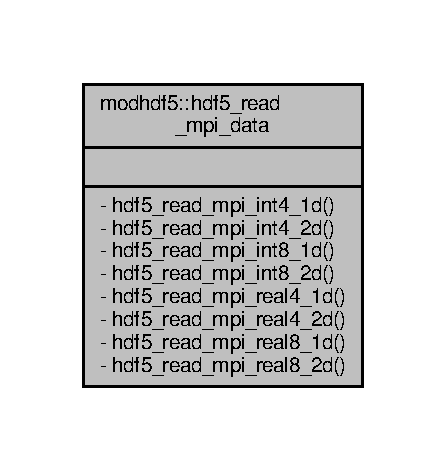
\includegraphics[width=214pt]{interfacemodhdf5_1_1hdf5__read__mpi__data__coll__graph}
\end{center}
\end{figure}
\subsection*{Private Member Functions}
\begin{DoxyCompactItemize}
\item 
subroutine \hyperlink{interfacemodhdf5_1_1hdf5__read__mpi__data_a1ad636a13c51c50de13eb1070aa325cc}{hdf5\+\_\+read\+\_\+mpi\+\_\+int4\+\_\+1d} (id, name, n1, data, comm)
\begin{DoxyCompactList}\small\item\em Read a 1-\/D integer4 array from a parallel file The array is distributed along the 2nd dimension. \end{DoxyCompactList}\item 
subroutine \hyperlink{interfacemodhdf5_1_1hdf5__read__mpi__data_adb25b404c7babd67561b609444f8b372}{hdf5\+\_\+read\+\_\+mpi\+\_\+int4\+\_\+2d} (id, name, n1, n2, data, comm)
\begin{DoxyCompactList}\small\item\em Read a 2-\/D integer4 array from a parallel file The array is distributed along the 2nd dimension. \end{DoxyCompactList}\item 
subroutine \hyperlink{interfacemodhdf5_1_1hdf5__read__mpi__data_a5a546e3a8ad2c01aa03f85ff9225d0ca}{hdf5\+\_\+read\+\_\+mpi\+\_\+int8\+\_\+1d} (id, name, n1, data, comm)
\begin{DoxyCompactList}\small\item\em Read a 1-\/D integer8 array from a parallel file The array is distributed along the 2nd dimension. \end{DoxyCompactList}\item 
subroutine \hyperlink{interfacemodhdf5_1_1hdf5__read__mpi__data_a7dcef34e2058f35d081d1c9b38269c6d}{hdf5\+\_\+read\+\_\+mpi\+\_\+int8\+\_\+2d} (id, name, n1, n2, data, comm)
\begin{DoxyCompactList}\small\item\em Read a 2-\/D integer8 array from a parallel file The array is distributed along the 2nd dimension. \end{DoxyCompactList}\item 
subroutine \hyperlink{interfacemodhdf5_1_1hdf5__read__mpi__data_a207ca36c3b403b84d6252beab44f0272}{hdf5\+\_\+read\+\_\+mpi\+\_\+real4\+\_\+1d} (id, name, n1, data, comm)
\begin{DoxyCompactList}\small\item\em Read a 1-\/D real4 array from a parallel file The array is distributed along the 2nd dimension. \end{DoxyCompactList}\item 
subroutine \hyperlink{interfacemodhdf5_1_1hdf5__read__mpi__data_afcd313f21020a6bd350c3ef9d3124868}{hdf5\+\_\+read\+\_\+mpi\+\_\+real4\+\_\+2d} (id, name, n1, n2, data, comm)
\begin{DoxyCompactList}\small\item\em Read a 2-\/D real4 array from a parallel file The array is distributed along the 2nd dimension. \end{DoxyCompactList}\item 
subroutine \hyperlink{interfacemodhdf5_1_1hdf5__read__mpi__data_a7097ac528961c8cfdc112324af9f7d0a}{hdf5\+\_\+read\+\_\+mpi\+\_\+real8\+\_\+1d} (id, name, n1, data, comm)
\begin{DoxyCompactList}\small\item\em Read a 1-\/D real8 array from a parallel file The array is distributed along the 2nd dimension. \end{DoxyCompactList}\item 
subroutine \hyperlink{interfacemodhdf5_1_1hdf5__read__mpi__data_a74c0e891094e9bc27d528af34a0f2045}{hdf5\+\_\+read\+\_\+mpi\+\_\+real8\+\_\+2d} (id, name, n1, n2, data, comm)
\begin{DoxyCompactList}\small\item\em Read a 2-\/D real8 array from a parallel file The array is distributed along the 2nd dimension. \end{DoxyCompactList}\end{DoxyCompactItemize}


\subsection{Detailed Description}
Generic inteface used to read data from a parallel hdf5 file. 


\begin{DoxyParams}[1]{Parameters}
\mbox{\tt in}  & {\em id} & id of the file/group where the dataset will be read \\
\hline
\mbox{\tt in}  & {\em name} & name of the dataset \\
\hline
\mbox{\tt in}  & {\em n1} & first dimension of the data array \\
\hline
\mbox{\tt in}  & {\em n2} & second dimension of the data array (optional) \\
\hline
\mbox{\tt in,out}  & {\em data} & 1-\/D or 2-\/D data array of type Integer(4), Integer(8), Real(4) or Real(8) \\
\hline
\mbox{\tt in}  & {\em comm} & M\+PI communicator used for the input (the same communicator should have been used to open the file) \\
\hline
\end{DoxyParams}


Definition at line 143 of file modhdf5.\+f90.



\subsection{Member Function/\+Subroutine Documentation}
\index{modhdf5\+::hdf5\+\_\+read\+\_\+mpi\+\_\+data@{modhdf5\+::hdf5\+\_\+read\+\_\+mpi\+\_\+data}!hdf5\+\_\+read\+\_\+mpi\+\_\+int4\+\_\+1d@{hdf5\+\_\+read\+\_\+mpi\+\_\+int4\+\_\+1d}}
\index{hdf5\+\_\+read\+\_\+mpi\+\_\+int4\+\_\+1d@{hdf5\+\_\+read\+\_\+mpi\+\_\+int4\+\_\+1d}!modhdf5\+::hdf5\+\_\+read\+\_\+mpi\+\_\+data@{modhdf5\+::hdf5\+\_\+read\+\_\+mpi\+\_\+data}}
\subsubsection[{\texorpdfstring{hdf5\+\_\+read\+\_\+mpi\+\_\+int4\+\_\+1d(id, name, n1, data, comm)}{hdf5_read_mpi_int4_1d(id, name, n1, data, comm)}}]{\setlength{\rightskip}{0pt plus 5cm}subroutine modhdf5\+::hdf5\+\_\+read\+\_\+mpi\+\_\+data\+::hdf5\+\_\+read\+\_\+mpi\+\_\+int4\+\_\+1d (
\begin{DoxyParamCaption}
\item[{integer(hid\+\_\+t), intent(in)}]{id, }
\item[{character(len={\bf h5strlen}), intent(in)}]{name, }
\item[{integer(kind=4), intent(in)}]{n1, }
\item[{integer(kind=4), dimension(n1), intent(inout), target}]{data, }
\item[{integer(kind=4), intent(in)}]{comm}
\end{DoxyParamCaption}
)\hspace{0.3cm}{\ttfamily [private]}}\hypertarget{interfacemodhdf5_1_1hdf5__read__mpi__data_a1ad636a13c51c50de13eb1070aa325cc}{}\label{interfacemodhdf5_1_1hdf5__read__mpi__data_a1ad636a13c51c50de13eb1070aa325cc}


Read a 1-\/D integer4 array from a parallel file The array is distributed along the 2nd dimension. 


\begin{DoxyParams}[1]{Parameters}
\mbox{\tt in}  & {\em id} & id of the file/group where the dataset will be read\\
\hline
\mbox{\tt in}  & {\em name} & name of the dataset\\
\hline
\mbox{\tt in}  & {\em n1} & dimension of the local array to read\\
\hline
\mbox{\tt in,out}  & {\em data} & array\\
\hline
\mbox{\tt in}  & {\em comm} & M\+PI communicator used \\
\hline
\end{DoxyParams}


Definition at line 2035 of file modhdf5.\+f90.

\index{modhdf5\+::hdf5\+\_\+read\+\_\+mpi\+\_\+data@{modhdf5\+::hdf5\+\_\+read\+\_\+mpi\+\_\+data}!hdf5\+\_\+read\+\_\+mpi\+\_\+int4\+\_\+2d@{hdf5\+\_\+read\+\_\+mpi\+\_\+int4\+\_\+2d}}
\index{hdf5\+\_\+read\+\_\+mpi\+\_\+int4\+\_\+2d@{hdf5\+\_\+read\+\_\+mpi\+\_\+int4\+\_\+2d}!modhdf5\+::hdf5\+\_\+read\+\_\+mpi\+\_\+data@{modhdf5\+::hdf5\+\_\+read\+\_\+mpi\+\_\+data}}
\subsubsection[{\texorpdfstring{hdf5\+\_\+read\+\_\+mpi\+\_\+int4\+\_\+2d(id, name, n1, n2, data, comm)}{hdf5_read_mpi_int4_2d(id, name, n1, n2, data, comm)}}]{\setlength{\rightskip}{0pt plus 5cm}subroutine modhdf5\+::hdf5\+\_\+read\+\_\+mpi\+\_\+data\+::hdf5\+\_\+read\+\_\+mpi\+\_\+int4\+\_\+2d (
\begin{DoxyParamCaption}
\item[{integer(hid\+\_\+t), intent(in)}]{id, }
\item[{character(len={\bf h5strlen}), intent(in)}]{name, }
\item[{integer(kind=4), intent(in)}]{n1, }
\item[{integer(kind=4), intent(in)}]{n2, }
\item[{integer(kind=4), dimension(n1,n2), intent(inout), target}]{data, }
\item[{integer(kind=4), intent(in)}]{comm}
\end{DoxyParamCaption}
)\hspace{0.3cm}{\ttfamily [private]}}\hypertarget{interfacemodhdf5_1_1hdf5__read__mpi__data_adb25b404c7babd67561b609444f8b372}{}\label{interfacemodhdf5_1_1hdf5__read__mpi__data_adb25b404c7babd67561b609444f8b372}


Read a 2-\/D integer4 array from a parallel file The array is distributed along the 2nd dimension. 


\begin{DoxyParams}[1]{Parameters}
\mbox{\tt in}  & {\em id} & id of the file/group where the dataset will be read\\
\hline
\mbox{\tt in}  & {\em name} & name of the dataset\\
\hline
\mbox{\tt in}  & {\em n1} & first dimension of the local array to read\\
\hline
\mbox{\tt in}  & {\em n2} & second dimension of the local array to read\\
\hline
\mbox{\tt in,out}  & {\em data} & array\\
\hline
\mbox{\tt in}  & {\em comm} & M\+PI communicator used \\
\hline
\end{DoxyParams}


Definition at line 2111 of file modhdf5.\+f90.

\index{modhdf5\+::hdf5\+\_\+read\+\_\+mpi\+\_\+data@{modhdf5\+::hdf5\+\_\+read\+\_\+mpi\+\_\+data}!hdf5\+\_\+read\+\_\+mpi\+\_\+int8\+\_\+1d@{hdf5\+\_\+read\+\_\+mpi\+\_\+int8\+\_\+1d}}
\index{hdf5\+\_\+read\+\_\+mpi\+\_\+int8\+\_\+1d@{hdf5\+\_\+read\+\_\+mpi\+\_\+int8\+\_\+1d}!modhdf5\+::hdf5\+\_\+read\+\_\+mpi\+\_\+data@{modhdf5\+::hdf5\+\_\+read\+\_\+mpi\+\_\+data}}
\subsubsection[{\texorpdfstring{hdf5\+\_\+read\+\_\+mpi\+\_\+int8\+\_\+1d(id, name, n1, data, comm)}{hdf5_read_mpi_int8_1d(id, name, n1, data, comm)}}]{\setlength{\rightskip}{0pt plus 5cm}subroutine modhdf5\+::hdf5\+\_\+read\+\_\+mpi\+\_\+data\+::hdf5\+\_\+read\+\_\+mpi\+\_\+int8\+\_\+1d (
\begin{DoxyParamCaption}
\item[{integer(hid\+\_\+t), intent(in)}]{id, }
\item[{character(len={\bf h5strlen}), intent(in)}]{name, }
\item[{integer(kind=4), intent(in)}]{n1, }
\item[{integer(kind=8), dimension(n1), intent(inout), target}]{data, }
\item[{integer(kind=4), intent(in)}]{comm}
\end{DoxyParamCaption}
)\hspace{0.3cm}{\ttfamily [private]}}\hypertarget{interfacemodhdf5_1_1hdf5__read__mpi__data_a5a546e3a8ad2c01aa03f85ff9225d0ca}{}\label{interfacemodhdf5_1_1hdf5__read__mpi__data_a5a546e3a8ad2c01aa03f85ff9225d0ca}


Read a 1-\/D integer8 array from a parallel file The array is distributed along the 2nd dimension. 


\begin{DoxyParams}[1]{Parameters}
\mbox{\tt in}  & {\em id} & id of the file/group where the dataset will be read\\
\hline
\mbox{\tt in}  & {\em name} & name of the dataset\\
\hline
\mbox{\tt in}  & {\em n1} & dimension of the local array to read\\
\hline
\mbox{\tt in,out}  & {\em data} & array\\
\hline
\mbox{\tt in}  & {\em comm} & M\+PI communicator used \\
\hline
\end{DoxyParams}


Definition at line 2191 of file modhdf5.\+f90.

\index{modhdf5\+::hdf5\+\_\+read\+\_\+mpi\+\_\+data@{modhdf5\+::hdf5\+\_\+read\+\_\+mpi\+\_\+data}!hdf5\+\_\+read\+\_\+mpi\+\_\+int8\+\_\+2d@{hdf5\+\_\+read\+\_\+mpi\+\_\+int8\+\_\+2d}}
\index{hdf5\+\_\+read\+\_\+mpi\+\_\+int8\+\_\+2d@{hdf5\+\_\+read\+\_\+mpi\+\_\+int8\+\_\+2d}!modhdf5\+::hdf5\+\_\+read\+\_\+mpi\+\_\+data@{modhdf5\+::hdf5\+\_\+read\+\_\+mpi\+\_\+data}}
\subsubsection[{\texorpdfstring{hdf5\+\_\+read\+\_\+mpi\+\_\+int8\+\_\+2d(id, name, n1, n2, data, comm)}{hdf5_read_mpi_int8_2d(id, name, n1, n2, data, comm)}}]{\setlength{\rightskip}{0pt plus 5cm}subroutine modhdf5\+::hdf5\+\_\+read\+\_\+mpi\+\_\+data\+::hdf5\+\_\+read\+\_\+mpi\+\_\+int8\+\_\+2d (
\begin{DoxyParamCaption}
\item[{integer(hid\+\_\+t), intent(in)}]{id, }
\item[{character(len={\bf h5strlen}), intent(in)}]{name, }
\item[{integer(kind=4), intent(in)}]{n1, }
\item[{integer(kind=4), intent(in)}]{n2, }
\item[{integer(kind=8), dimension(n1,n2), intent(inout), target}]{data, }
\item[{integer(kind=4), intent(in)}]{comm}
\end{DoxyParamCaption}
)\hspace{0.3cm}{\ttfamily [private]}}\hypertarget{interfacemodhdf5_1_1hdf5__read__mpi__data_a7dcef34e2058f35d081d1c9b38269c6d}{}\label{interfacemodhdf5_1_1hdf5__read__mpi__data_a7dcef34e2058f35d081d1c9b38269c6d}


Read a 2-\/D integer8 array from a parallel file The array is distributed along the 2nd dimension. 


\begin{DoxyParams}[1]{Parameters}
\mbox{\tt in}  & {\em id} & id of the file/group where the dataset will be read\\
\hline
\mbox{\tt in}  & {\em name} & name of the dataset\\
\hline
\mbox{\tt in}  & {\em n1} & first dimension of the local array to read\\
\hline
\mbox{\tt in}  & {\em n2} & second dimension of the local array to read\\
\hline
\mbox{\tt in,out}  & {\em data} & array\\
\hline
\mbox{\tt in}  & {\em comm} & M\+PI communicator used \\
\hline
\end{DoxyParams}


Definition at line 2268 of file modhdf5.\+f90.

\index{modhdf5\+::hdf5\+\_\+read\+\_\+mpi\+\_\+data@{modhdf5\+::hdf5\+\_\+read\+\_\+mpi\+\_\+data}!hdf5\+\_\+read\+\_\+mpi\+\_\+real4\+\_\+1d@{hdf5\+\_\+read\+\_\+mpi\+\_\+real4\+\_\+1d}}
\index{hdf5\+\_\+read\+\_\+mpi\+\_\+real4\+\_\+1d@{hdf5\+\_\+read\+\_\+mpi\+\_\+real4\+\_\+1d}!modhdf5\+::hdf5\+\_\+read\+\_\+mpi\+\_\+data@{modhdf5\+::hdf5\+\_\+read\+\_\+mpi\+\_\+data}}
\subsubsection[{\texorpdfstring{hdf5\+\_\+read\+\_\+mpi\+\_\+real4\+\_\+1d(id, name, n1, data, comm)}{hdf5_read_mpi_real4_1d(id, name, n1, data, comm)}}]{\setlength{\rightskip}{0pt plus 5cm}subroutine modhdf5\+::hdf5\+\_\+read\+\_\+mpi\+\_\+data\+::hdf5\+\_\+read\+\_\+mpi\+\_\+real4\+\_\+1d (
\begin{DoxyParamCaption}
\item[{integer(hid\+\_\+t), intent(in)}]{id, }
\item[{character(len={\bf h5strlen}), intent(in)}]{name, }
\item[{integer(kind=4), intent(in)}]{n1, }
\item[{real(kind=4), dimension(n1), intent(inout), target}]{data, }
\item[{integer(kind=4), intent(in)}]{comm}
\end{DoxyParamCaption}
)\hspace{0.3cm}{\ttfamily [private]}}\hypertarget{interfacemodhdf5_1_1hdf5__read__mpi__data_a207ca36c3b403b84d6252beab44f0272}{}\label{interfacemodhdf5_1_1hdf5__read__mpi__data_a207ca36c3b403b84d6252beab44f0272}


Read a 1-\/D real4 array from a parallel file The array is distributed along the 2nd dimension. 


\begin{DoxyParams}[1]{Parameters}
\mbox{\tt in}  & {\em id} & id of the file/group where the dataset will be read\\
\hline
\mbox{\tt in}  & {\em name} & name of the dataset\\
\hline
\mbox{\tt in}  & {\em n1} & dimension of the local array to read\\
\hline
\mbox{\tt in,out}  & {\em data} & array\\
\hline
\mbox{\tt in}  & {\em comm} & M\+PI communicator used \\
\hline
\end{DoxyParams}


Definition at line 2348 of file modhdf5.\+f90.

\index{modhdf5\+::hdf5\+\_\+read\+\_\+mpi\+\_\+data@{modhdf5\+::hdf5\+\_\+read\+\_\+mpi\+\_\+data}!hdf5\+\_\+read\+\_\+mpi\+\_\+real4\+\_\+2d@{hdf5\+\_\+read\+\_\+mpi\+\_\+real4\+\_\+2d}}
\index{hdf5\+\_\+read\+\_\+mpi\+\_\+real4\+\_\+2d@{hdf5\+\_\+read\+\_\+mpi\+\_\+real4\+\_\+2d}!modhdf5\+::hdf5\+\_\+read\+\_\+mpi\+\_\+data@{modhdf5\+::hdf5\+\_\+read\+\_\+mpi\+\_\+data}}
\subsubsection[{\texorpdfstring{hdf5\+\_\+read\+\_\+mpi\+\_\+real4\+\_\+2d(id, name, n1, n2, data, comm)}{hdf5_read_mpi_real4_2d(id, name, n1, n2, data, comm)}}]{\setlength{\rightskip}{0pt plus 5cm}subroutine modhdf5\+::hdf5\+\_\+read\+\_\+mpi\+\_\+data\+::hdf5\+\_\+read\+\_\+mpi\+\_\+real4\+\_\+2d (
\begin{DoxyParamCaption}
\item[{integer(hid\+\_\+t), intent(in)}]{id, }
\item[{character(len={\bf h5strlen}), intent(in)}]{name, }
\item[{integer(kind=4), intent(in)}]{n1, }
\item[{integer(kind=4), intent(in)}]{n2, }
\item[{real(kind=4), dimension(n1,n2), intent(inout), target}]{data, }
\item[{integer(kind=4), intent(in)}]{comm}
\end{DoxyParamCaption}
)\hspace{0.3cm}{\ttfamily [private]}}\hypertarget{interfacemodhdf5_1_1hdf5__read__mpi__data_afcd313f21020a6bd350c3ef9d3124868}{}\label{interfacemodhdf5_1_1hdf5__read__mpi__data_afcd313f21020a6bd350c3ef9d3124868}


Read a 2-\/D real4 array from a parallel file The array is distributed along the 2nd dimension. 


\begin{DoxyParams}[1]{Parameters}
\mbox{\tt in}  & {\em id} & id of the file/group where the dataset will be read\\
\hline
\mbox{\tt in}  & {\em name} & name of the dataset\\
\hline
\mbox{\tt in}  & {\em n1} & first dimension of the local array to read\\
\hline
\mbox{\tt in}  & {\em n2} & second dimension of the local array to read\\
\hline
\mbox{\tt in,out}  & {\em data} & array\\
\hline
\mbox{\tt in}  & {\em comm} & M\+PI communicator used \\
\hline
\end{DoxyParams}


Definition at line 2424 of file modhdf5.\+f90.

\index{modhdf5\+::hdf5\+\_\+read\+\_\+mpi\+\_\+data@{modhdf5\+::hdf5\+\_\+read\+\_\+mpi\+\_\+data}!hdf5\+\_\+read\+\_\+mpi\+\_\+real8\+\_\+1d@{hdf5\+\_\+read\+\_\+mpi\+\_\+real8\+\_\+1d}}
\index{hdf5\+\_\+read\+\_\+mpi\+\_\+real8\+\_\+1d@{hdf5\+\_\+read\+\_\+mpi\+\_\+real8\+\_\+1d}!modhdf5\+::hdf5\+\_\+read\+\_\+mpi\+\_\+data@{modhdf5\+::hdf5\+\_\+read\+\_\+mpi\+\_\+data}}
\subsubsection[{\texorpdfstring{hdf5\+\_\+read\+\_\+mpi\+\_\+real8\+\_\+1d(id, name, n1, data, comm)}{hdf5_read_mpi_real8_1d(id, name, n1, data, comm)}}]{\setlength{\rightskip}{0pt plus 5cm}subroutine modhdf5\+::hdf5\+\_\+read\+\_\+mpi\+\_\+data\+::hdf5\+\_\+read\+\_\+mpi\+\_\+real8\+\_\+1d (
\begin{DoxyParamCaption}
\item[{integer(hid\+\_\+t), intent(in)}]{id, }
\item[{character(len={\bf h5strlen}), intent(in)}]{name, }
\item[{integer(kind=4), intent(in)}]{n1, }
\item[{real(kind=8), dimension(n1), intent(inout), target}]{data, }
\item[{integer(kind=4), intent(in)}]{comm}
\end{DoxyParamCaption}
)\hspace{0.3cm}{\ttfamily [private]}}\hypertarget{interfacemodhdf5_1_1hdf5__read__mpi__data_a7097ac528961c8cfdc112324af9f7d0a}{}\label{interfacemodhdf5_1_1hdf5__read__mpi__data_a7097ac528961c8cfdc112324af9f7d0a}


Read a 1-\/D real8 array from a parallel file The array is distributed along the 2nd dimension. 


\begin{DoxyParams}[1]{Parameters}
\mbox{\tt in}  & {\em id} & id of the file/group where the dataset will be read\\
\hline
\mbox{\tt in}  & {\em name} & name of the dataset\\
\hline
\mbox{\tt in}  & {\em n1} & dimension of the local array to read\\
\hline
\mbox{\tt in,out}  & {\em data} & array\\
\hline
\mbox{\tt in}  & {\em comm} & M\+PI communicator used \\
\hline
\end{DoxyParams}


Definition at line 2508 of file modhdf5.\+f90.

\index{modhdf5\+::hdf5\+\_\+read\+\_\+mpi\+\_\+data@{modhdf5\+::hdf5\+\_\+read\+\_\+mpi\+\_\+data}!hdf5\+\_\+read\+\_\+mpi\+\_\+real8\+\_\+2d@{hdf5\+\_\+read\+\_\+mpi\+\_\+real8\+\_\+2d}}
\index{hdf5\+\_\+read\+\_\+mpi\+\_\+real8\+\_\+2d@{hdf5\+\_\+read\+\_\+mpi\+\_\+real8\+\_\+2d}!modhdf5\+::hdf5\+\_\+read\+\_\+mpi\+\_\+data@{modhdf5\+::hdf5\+\_\+read\+\_\+mpi\+\_\+data}}
\subsubsection[{\texorpdfstring{hdf5\+\_\+read\+\_\+mpi\+\_\+real8\+\_\+2d(id, name, n1, n2, data, comm)}{hdf5_read_mpi_real8_2d(id, name, n1, n2, data, comm)}}]{\setlength{\rightskip}{0pt plus 5cm}subroutine modhdf5\+::hdf5\+\_\+read\+\_\+mpi\+\_\+data\+::hdf5\+\_\+read\+\_\+mpi\+\_\+real8\+\_\+2d (
\begin{DoxyParamCaption}
\item[{integer(hid\+\_\+t), intent(in)}]{id, }
\item[{character(len={\bf h5strlen}), intent(in)}]{name, }
\item[{integer(kind=4), intent(in)}]{n1, }
\item[{integer(kind=4), intent(in)}]{n2, }
\item[{real(kind=8), dimension(n1,n2), intent(inout), target}]{data, }
\item[{integer(kind=4), intent(in)}]{comm}
\end{DoxyParamCaption}
)\hspace{0.3cm}{\ttfamily [private]}}\hypertarget{interfacemodhdf5_1_1hdf5__read__mpi__data_a74c0e891094e9bc27d528af34a0f2045}{}\label{interfacemodhdf5_1_1hdf5__read__mpi__data_a74c0e891094e9bc27d528af34a0f2045}


Read a 2-\/D real8 array from a parallel file The array is distributed along the 2nd dimension. 


\begin{DoxyParams}[1]{Parameters}
\mbox{\tt in}  & {\em id} & id of the file/group where the dataset will be read\\
\hline
\mbox{\tt in}  & {\em name} & name of the dataset\\
\hline
\mbox{\tt in}  & {\em n1} & first dimension of the local array to read\\
\hline
\mbox{\tt in}  & {\em n2} & second dimension of the local array to read\\
\hline
\mbox{\tt in,out}  & {\em data} & array\\
\hline
\mbox{\tt in}  & {\em comm} & M\+PI communicator used \\
\hline
\end{DoxyParams}


Definition at line 2585 of file modhdf5.\+f90.



The documentation for this interface was generated from the following file\+:\begin{DoxyCompactItemize}
\item 
/home/roy/\+Travail/\+Devel/\+Cosmologie/\+Pfof/trunk/common/src/\hyperlink{modhdf5_8f90}{modhdf5.\+f90}\end{DoxyCompactItemize}

\hypertarget{interfacemodhdf5_1_1hdf5__write__attr}{}\section{modhdf5\+:\+:hdf5\+\_\+write\+\_\+attr Interface Reference}
\label{interfacemodhdf5_1_1hdf5__write__attr}\index{modhdf5\+::hdf5\+\_\+write\+\_\+attr@{modhdf5\+::hdf5\+\_\+write\+\_\+attr}}


Generic inteface used to write attributes in a hdf5 file.  




Collaboration diagram for modhdf5\+:\+:hdf5\+\_\+write\+\_\+attr\+:\nopagebreak
\begin{figure}[H]
\begin{center}
\leavevmode
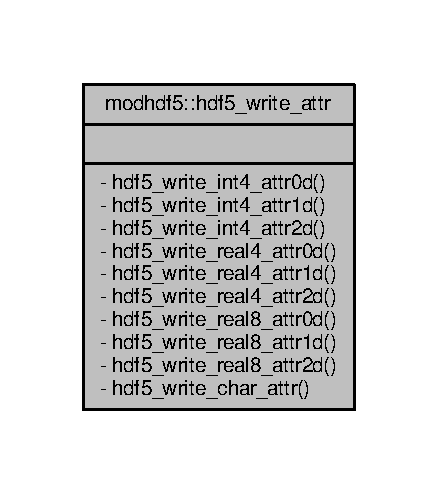
\includegraphics[width=210pt]{interfacemodhdf5_1_1hdf5__write__attr__coll__graph}
\end{center}
\end{figure}
\subsection*{Private Member Functions}
\begin{DoxyCompactItemize}
\item 
subroutine \hyperlink{interfacemodhdf5_1_1hdf5__write__attr_a3959ef2486c4c456e76584168da85aba}{hdf5\+\_\+write\+\_\+int4\+\_\+attr0d} (id, name, data)
\begin{DoxyCompactList}\small\item\em Write an integer4 as attribute. \end{DoxyCompactList}\item 
subroutine \hyperlink{interfacemodhdf5_1_1hdf5__write__attr_aa621d5efc77049d6ee8dab8b8a1e7ebe}{hdf5\+\_\+write\+\_\+int4\+\_\+attr1d} (id, name, n1, data)
\begin{DoxyCompactList}\small\item\em Write a 1-\/D array of integer4 as attribute. \end{DoxyCompactList}\item 
subroutine \hyperlink{interfacemodhdf5_1_1hdf5__write__attr_a38454d655e553e07bfaba67da14fd578}{hdf5\+\_\+write\+\_\+int4\+\_\+attr2d} (id, name, n1, n2, data)
\item 
subroutine \hyperlink{interfacemodhdf5_1_1hdf5__write__attr_adb6eff5c1284cf4fed9bd8a331a219fd}{hdf5\+\_\+write\+\_\+real4\+\_\+attr0d} (id, name, data)
\begin{DoxyCompactList}\small\item\em Write a real4 as attribute. \end{DoxyCompactList}\item 
subroutine \hyperlink{interfacemodhdf5_1_1hdf5__write__attr_a962f1050530d43822075bb646e631411}{hdf5\+\_\+write\+\_\+real4\+\_\+attr1d} (id, name, n1, data)
\begin{DoxyCompactList}\small\item\em Write a 1-\/D array of real4 as attribute. \end{DoxyCompactList}\item 
subroutine \hyperlink{interfacemodhdf5_1_1hdf5__write__attr_aae8bb567dcb75727d39619cfae14043f}{hdf5\+\_\+write\+\_\+real4\+\_\+attr2d} (id, name, n1, n2, data)
\item 
subroutine \hyperlink{interfacemodhdf5_1_1hdf5__write__attr_a867dca47b84260259e3a7fef99298dc8}{hdf5\+\_\+write\+\_\+real8\+\_\+attr0d} (id, name, data)
\begin{DoxyCompactList}\small\item\em Write a real8 as attribute. \end{DoxyCompactList}\item 
subroutine \hyperlink{interfacemodhdf5_1_1hdf5__write__attr_a105da78bee8590ebd4014d9950b2251f}{hdf5\+\_\+write\+\_\+real8\+\_\+attr1d} (id, name, n1, data)
\begin{DoxyCompactList}\small\item\em Write a 1-\/D array of real8 as attribute. \end{DoxyCompactList}\item 
subroutine \hyperlink{interfacemodhdf5_1_1hdf5__write__attr_ad858843f21c092410756a7b22d504c40}{hdf5\+\_\+write\+\_\+real8\+\_\+attr2d} (id, name, n1, n2, data)
\item 
subroutine \hyperlink{interfacemodhdf5_1_1hdf5__write__attr_a8f365b16166c853d262252695f699d76}{hdf5\+\_\+write\+\_\+char\+\_\+attr} (id, name, data)
\begin{DoxyCompactList}\small\item\em Write a string as attribute. \end{DoxyCompactList}\end{DoxyCompactItemize}


\subsection{Detailed Description}
Generic inteface used to write attributes in a hdf5 file. 


\begin{DoxyParams}[1]{Parameters}
\mbox{\tt in}  & {\em id} & id of the file/group where the attribute will be written \\
\hline
\mbox{\tt in}  & {\em name} & name of the attribute \\
\hline
\mbox{\tt in}  & {\em n1} & first dimension of the attribute array (optional) \\
\hline
\mbox{\tt in}  & {\em n2} & second dimension of the attribute array (optional) \\
\hline
\mbox{\tt in}  & {\em data} & 0-\/D, 1-\/D or 2-\/D attribute of type Integer(4), Real(4), Real(8) or Character \\
\hline
\end{DoxyParams}


Definition at line 50 of file modhdf5.\+f90.



\subsection{Member Function/\+Subroutine Documentation}
\index{modhdf5\+::hdf5\+\_\+write\+\_\+attr@{modhdf5\+::hdf5\+\_\+write\+\_\+attr}!hdf5\+\_\+write\+\_\+char\+\_\+attr@{hdf5\+\_\+write\+\_\+char\+\_\+attr}}
\index{hdf5\+\_\+write\+\_\+char\+\_\+attr@{hdf5\+\_\+write\+\_\+char\+\_\+attr}!modhdf5\+::hdf5\+\_\+write\+\_\+attr@{modhdf5\+::hdf5\+\_\+write\+\_\+attr}}
\subsubsection[{\texorpdfstring{hdf5\+\_\+write\+\_\+char\+\_\+attr(id, name, data)}{hdf5_write_char_attr(id, name, data)}}]{\setlength{\rightskip}{0pt plus 5cm}subroutine modhdf5\+::hdf5\+\_\+write\+\_\+attr\+::hdf5\+\_\+write\+\_\+char\+\_\+attr (
\begin{DoxyParamCaption}
\item[{integer(hid\+\_\+t), intent(in)}]{id, }
\item[{character(len={\bf h5strlen}), intent(in)}]{name, }
\item[{character($\ast$), intent(in)}]{data}
\end{DoxyParamCaption}
)\hspace{0.3cm}{\ttfamily [private]}}\hypertarget{interfacemodhdf5_1_1hdf5__write__attr_a8f365b16166c853d262252695f699d76}{}\label{interfacemodhdf5_1_1hdf5__write__attr_a8f365b16166c853d262252695f699d76}


Write a string as attribute. 


\begin{DoxyParams}[1]{Parameters}
\mbox{\tt in}  & {\em id} & id of the file/group where the attribute will be written\\
\hline
\mbox{\tt in}  & {\em name} & name of the attribute\\
\hline
\mbox{\tt in}  & {\em data} & attribute value \\
\hline
\end{DoxyParams}


Definition at line 2992 of file modhdf5.\+f90.

\index{modhdf5\+::hdf5\+\_\+write\+\_\+attr@{modhdf5\+::hdf5\+\_\+write\+\_\+attr}!hdf5\+\_\+write\+\_\+int4\+\_\+attr0d@{hdf5\+\_\+write\+\_\+int4\+\_\+attr0d}}
\index{hdf5\+\_\+write\+\_\+int4\+\_\+attr0d@{hdf5\+\_\+write\+\_\+int4\+\_\+attr0d}!modhdf5\+::hdf5\+\_\+write\+\_\+attr@{modhdf5\+::hdf5\+\_\+write\+\_\+attr}}
\subsubsection[{\texorpdfstring{hdf5\+\_\+write\+\_\+int4\+\_\+attr0d(id, name, data)}{hdf5_write_int4_attr0d(id, name, data)}}]{\setlength{\rightskip}{0pt plus 5cm}subroutine modhdf5\+::hdf5\+\_\+write\+\_\+attr\+::hdf5\+\_\+write\+\_\+int4\+\_\+attr0d (
\begin{DoxyParamCaption}
\item[{integer(hid\+\_\+t), intent(in)}]{id, }
\item[{character(len={\bf h5strlen}), intent(in)}]{name, }
\item[{integer(kind=4), intent(in)}]{data}
\end{DoxyParamCaption}
)\hspace{0.3cm}{\ttfamily [private]}}\hypertarget{interfacemodhdf5_1_1hdf5__write__attr_a3959ef2486c4c456e76584168da85aba}{}\label{interfacemodhdf5_1_1hdf5__write__attr_a3959ef2486c4c456e76584168da85aba}


Write an integer4 as attribute. 


\begin{DoxyParams}[1]{Parameters}
\mbox{\tt in}  & {\em id} & id of the file/group where the attribute will be written\\
\hline
\mbox{\tt in}  & {\em name} & name of the attribute\\
\hline
\mbox{\tt in}  & {\em data} & attribute value \\
\hline
\end{DoxyParams}


Definition at line 2669 of file modhdf5.\+f90.

\index{modhdf5\+::hdf5\+\_\+write\+\_\+attr@{modhdf5\+::hdf5\+\_\+write\+\_\+attr}!hdf5\+\_\+write\+\_\+int4\+\_\+attr1d@{hdf5\+\_\+write\+\_\+int4\+\_\+attr1d}}
\index{hdf5\+\_\+write\+\_\+int4\+\_\+attr1d@{hdf5\+\_\+write\+\_\+int4\+\_\+attr1d}!modhdf5\+::hdf5\+\_\+write\+\_\+attr@{modhdf5\+::hdf5\+\_\+write\+\_\+attr}}
\subsubsection[{\texorpdfstring{hdf5\+\_\+write\+\_\+int4\+\_\+attr1d(id, name, n1, data)}{hdf5_write_int4_attr1d(id, name, n1, data)}}]{\setlength{\rightskip}{0pt plus 5cm}subroutine modhdf5\+::hdf5\+\_\+write\+\_\+attr\+::hdf5\+\_\+write\+\_\+int4\+\_\+attr1d (
\begin{DoxyParamCaption}
\item[{integer(hid\+\_\+t), intent(in)}]{id, }
\item[{character(len={\bf h5strlen}), intent(in)}]{name, }
\item[{integer(kind=4), intent(in)}]{n1, }
\item[{integer(kind=4), dimension(n1), intent(in)}]{data}
\end{DoxyParamCaption}
)\hspace{0.3cm}{\ttfamily [private]}}\hypertarget{interfacemodhdf5_1_1hdf5__write__attr_aa621d5efc77049d6ee8dab8b8a1e7ebe}{}\label{interfacemodhdf5_1_1hdf5__write__attr_aa621d5efc77049d6ee8dab8b8a1e7ebe}


Write a 1-\/D array of integer4 as attribute. 


\begin{DoxyParams}[1]{Parameters}
\mbox{\tt in}  & {\em id} & id of the file/group where the attribute will be written\\
\hline
\mbox{\tt in}  & {\em name} & name of the attribute\\
\hline
\mbox{\tt in}  & {\em n1} & dimension of the attribute array\\
\hline
\mbox{\tt in}  & {\em data} & attribute value \\
\hline
\end{DoxyParams}


Definition at line 2709 of file modhdf5.\+f90.

\index{modhdf5\+::hdf5\+\_\+write\+\_\+attr@{modhdf5\+::hdf5\+\_\+write\+\_\+attr}!hdf5\+\_\+write\+\_\+int4\+\_\+attr2d@{hdf5\+\_\+write\+\_\+int4\+\_\+attr2d}}
\index{hdf5\+\_\+write\+\_\+int4\+\_\+attr2d@{hdf5\+\_\+write\+\_\+int4\+\_\+attr2d}!modhdf5\+::hdf5\+\_\+write\+\_\+attr@{modhdf5\+::hdf5\+\_\+write\+\_\+attr}}
\subsubsection[{\texorpdfstring{hdf5\+\_\+write\+\_\+int4\+\_\+attr2d(id, name, n1, n2, data)}{hdf5_write_int4_attr2d(id, name, n1, n2, data)}}]{\setlength{\rightskip}{0pt plus 5cm}subroutine modhdf5\+::hdf5\+\_\+write\+\_\+attr\+::hdf5\+\_\+write\+\_\+int4\+\_\+attr2d (
\begin{DoxyParamCaption}
\item[{integer(hid\+\_\+t), intent(in)}]{id, }
\item[{character(len={\bf h5strlen}), intent(in)}]{name, }
\item[{integer(kind=4), intent(in)}]{n1, }
\item[{integer(kind=4), intent(in)}]{n2, }
\item[{integer(kind=4), dimension(n1,n2), intent(in)}]{data}
\end{DoxyParamCaption}
)\hspace{0.3cm}{\ttfamily [private]}}\hypertarget{interfacemodhdf5_1_1hdf5__write__attr_a38454d655e553e07bfaba67da14fd578}{}\label{interfacemodhdf5_1_1hdf5__write__attr_a38454d655e553e07bfaba67da14fd578}

\begin{DoxyParams}[1]{Parameters}
\mbox{\tt in}  & {\em id} & id of the file/group where the attribute will be written\\
\hline
\mbox{\tt in}  & {\em name} & name of the attribute\\
\hline
\mbox{\tt in}  & {\em n1} & first dimension of the attribute array\\
\hline
\mbox{\tt in}  & {\em n2} & second dimension of the attribute array\\
\hline
\mbox{\tt in}  & {\em data} & attribute value \\
\hline
\end{DoxyParams}


Definition at line 2744 of file modhdf5.\+f90.

\index{modhdf5\+::hdf5\+\_\+write\+\_\+attr@{modhdf5\+::hdf5\+\_\+write\+\_\+attr}!hdf5\+\_\+write\+\_\+real4\+\_\+attr0d@{hdf5\+\_\+write\+\_\+real4\+\_\+attr0d}}
\index{hdf5\+\_\+write\+\_\+real4\+\_\+attr0d@{hdf5\+\_\+write\+\_\+real4\+\_\+attr0d}!modhdf5\+::hdf5\+\_\+write\+\_\+attr@{modhdf5\+::hdf5\+\_\+write\+\_\+attr}}
\subsubsection[{\texorpdfstring{hdf5\+\_\+write\+\_\+real4\+\_\+attr0d(id, name, data)}{hdf5_write_real4_attr0d(id, name, data)}}]{\setlength{\rightskip}{0pt plus 5cm}subroutine modhdf5\+::hdf5\+\_\+write\+\_\+attr\+::hdf5\+\_\+write\+\_\+real4\+\_\+attr0d (
\begin{DoxyParamCaption}
\item[{integer(hid\+\_\+t), intent(in)}]{id, }
\item[{character(len={\bf h5strlen}), intent(in)}]{name, }
\item[{real(kind=4), intent(in)}]{data}
\end{DoxyParamCaption}
)\hspace{0.3cm}{\ttfamily [private]}}\hypertarget{interfacemodhdf5_1_1hdf5__write__attr_adb6eff5c1284cf4fed9bd8a331a219fd}{}\label{interfacemodhdf5_1_1hdf5__write__attr_adb6eff5c1284cf4fed9bd8a331a219fd}


Write a real4 as attribute. 


\begin{DoxyParams}[1]{Parameters}
\mbox{\tt in}  & {\em id} & id of the file/group where the attribute will be written\\
\hline
\mbox{\tt in}  & {\em name} & name of the attribute\\
\hline
\mbox{\tt in}  & {\em data} & attribute value \\
\hline
\end{DoxyParams}


Definition at line 2780 of file modhdf5.\+f90.

\index{modhdf5\+::hdf5\+\_\+write\+\_\+attr@{modhdf5\+::hdf5\+\_\+write\+\_\+attr}!hdf5\+\_\+write\+\_\+real4\+\_\+attr1d@{hdf5\+\_\+write\+\_\+real4\+\_\+attr1d}}
\index{hdf5\+\_\+write\+\_\+real4\+\_\+attr1d@{hdf5\+\_\+write\+\_\+real4\+\_\+attr1d}!modhdf5\+::hdf5\+\_\+write\+\_\+attr@{modhdf5\+::hdf5\+\_\+write\+\_\+attr}}
\subsubsection[{\texorpdfstring{hdf5\+\_\+write\+\_\+real4\+\_\+attr1d(id, name, n1, data)}{hdf5_write_real4_attr1d(id, name, n1, data)}}]{\setlength{\rightskip}{0pt plus 5cm}subroutine modhdf5\+::hdf5\+\_\+write\+\_\+attr\+::hdf5\+\_\+write\+\_\+real4\+\_\+attr1d (
\begin{DoxyParamCaption}
\item[{integer(hid\+\_\+t), intent(in)}]{id, }
\item[{character(len={\bf h5strlen}), intent(in)}]{name, }
\item[{integer(kind=4), intent(in)}]{n1, }
\item[{real(kind=4), dimension(n1), intent(in)}]{data}
\end{DoxyParamCaption}
)\hspace{0.3cm}{\ttfamily [private]}}\hypertarget{interfacemodhdf5_1_1hdf5__write__attr_a962f1050530d43822075bb646e631411}{}\label{interfacemodhdf5_1_1hdf5__write__attr_a962f1050530d43822075bb646e631411}


Write a 1-\/D array of real4 as attribute. 


\begin{DoxyParams}[1]{Parameters}
\mbox{\tt in}  & {\em id} & id of the file/group where the attribute will be written\\
\hline
\mbox{\tt in}  & {\em name} & name of the attribute\\
\hline
\mbox{\tt in}  & {\em n1} & dimension of the attribute array\\
\hline
\mbox{\tt in}  & {\em data} & attribute value \\
\hline
\end{DoxyParams}


Definition at line 2814 of file modhdf5.\+f90.

\index{modhdf5\+::hdf5\+\_\+write\+\_\+attr@{modhdf5\+::hdf5\+\_\+write\+\_\+attr}!hdf5\+\_\+write\+\_\+real4\+\_\+attr2d@{hdf5\+\_\+write\+\_\+real4\+\_\+attr2d}}
\index{hdf5\+\_\+write\+\_\+real4\+\_\+attr2d@{hdf5\+\_\+write\+\_\+real4\+\_\+attr2d}!modhdf5\+::hdf5\+\_\+write\+\_\+attr@{modhdf5\+::hdf5\+\_\+write\+\_\+attr}}
\subsubsection[{\texorpdfstring{hdf5\+\_\+write\+\_\+real4\+\_\+attr2d(id, name, n1, n2, data)}{hdf5_write_real4_attr2d(id, name, n1, n2, data)}}]{\setlength{\rightskip}{0pt plus 5cm}subroutine modhdf5\+::hdf5\+\_\+write\+\_\+attr\+::hdf5\+\_\+write\+\_\+real4\+\_\+attr2d (
\begin{DoxyParamCaption}
\item[{integer(hid\+\_\+t), intent(in)}]{id, }
\item[{character(len={\bf h5strlen}), intent(in)}]{name, }
\item[{integer(kind=4), intent(in)}]{n1, }
\item[{integer(kind=4), intent(in)}]{n2, }
\item[{real(kind=4), dimension(n1,n2), intent(in)}]{data}
\end{DoxyParamCaption}
)\hspace{0.3cm}{\ttfamily [private]}}\hypertarget{interfacemodhdf5_1_1hdf5__write__attr_aae8bb567dcb75727d39619cfae14043f}{}\label{interfacemodhdf5_1_1hdf5__write__attr_aae8bb567dcb75727d39619cfae14043f}

\begin{DoxyParams}[1]{Parameters}
\mbox{\tt in}  & {\em id} & id of the file/group where the attribute will be written\\
\hline
\mbox{\tt in}  & {\em name} & name of the attribute\\
\hline
\mbox{\tt in}  & {\em n1} & first dimension of the attribute array\\
\hline
\mbox{\tt in}  & {\em n2} & second dimension of the attribute array\\
\hline
\mbox{\tt in}  & {\em data} & attribute value \\
\hline
\end{DoxyParams}


Definition at line 2849 of file modhdf5.\+f90.

\index{modhdf5\+::hdf5\+\_\+write\+\_\+attr@{modhdf5\+::hdf5\+\_\+write\+\_\+attr}!hdf5\+\_\+write\+\_\+real8\+\_\+attr0d@{hdf5\+\_\+write\+\_\+real8\+\_\+attr0d}}
\index{hdf5\+\_\+write\+\_\+real8\+\_\+attr0d@{hdf5\+\_\+write\+\_\+real8\+\_\+attr0d}!modhdf5\+::hdf5\+\_\+write\+\_\+attr@{modhdf5\+::hdf5\+\_\+write\+\_\+attr}}
\subsubsection[{\texorpdfstring{hdf5\+\_\+write\+\_\+real8\+\_\+attr0d(id, name, data)}{hdf5_write_real8_attr0d(id, name, data)}}]{\setlength{\rightskip}{0pt plus 5cm}subroutine modhdf5\+::hdf5\+\_\+write\+\_\+attr\+::hdf5\+\_\+write\+\_\+real8\+\_\+attr0d (
\begin{DoxyParamCaption}
\item[{integer(hid\+\_\+t), intent(in)}]{id, }
\item[{character(len={\bf h5strlen}), intent(in)}]{name, }
\item[{real(kind=8), intent(in)}]{data}
\end{DoxyParamCaption}
)\hspace{0.3cm}{\ttfamily [private]}}\hypertarget{interfacemodhdf5_1_1hdf5__write__attr_a867dca47b84260259e3a7fef99298dc8}{}\label{interfacemodhdf5_1_1hdf5__write__attr_a867dca47b84260259e3a7fef99298dc8}


Write a real8 as attribute. 


\begin{DoxyParams}[1]{Parameters}
\mbox{\tt in}  & {\em id} & id of the file/group where the attribute will be written\\
\hline
\mbox{\tt in}  & {\em name} & name of the attribute\\
\hline
\mbox{\tt in}  & {\em data} & attribute value \\
\hline
\end{DoxyParams}


Definition at line 2886 of file modhdf5.\+f90.

\index{modhdf5\+::hdf5\+\_\+write\+\_\+attr@{modhdf5\+::hdf5\+\_\+write\+\_\+attr}!hdf5\+\_\+write\+\_\+real8\+\_\+attr1d@{hdf5\+\_\+write\+\_\+real8\+\_\+attr1d}}
\index{hdf5\+\_\+write\+\_\+real8\+\_\+attr1d@{hdf5\+\_\+write\+\_\+real8\+\_\+attr1d}!modhdf5\+::hdf5\+\_\+write\+\_\+attr@{modhdf5\+::hdf5\+\_\+write\+\_\+attr}}
\subsubsection[{\texorpdfstring{hdf5\+\_\+write\+\_\+real8\+\_\+attr1d(id, name, n1, data)}{hdf5_write_real8_attr1d(id, name, n1, data)}}]{\setlength{\rightskip}{0pt plus 5cm}subroutine modhdf5\+::hdf5\+\_\+write\+\_\+attr\+::hdf5\+\_\+write\+\_\+real8\+\_\+attr1d (
\begin{DoxyParamCaption}
\item[{integer(hid\+\_\+t), intent(in)}]{id, }
\item[{character(len={\bf h5strlen}), intent(in)}]{name, }
\item[{integer(kind=4), intent(in)}]{n1, }
\item[{real(kind=8), dimension(n1), intent(in)}]{data}
\end{DoxyParamCaption}
)\hspace{0.3cm}{\ttfamily [private]}}\hypertarget{interfacemodhdf5_1_1hdf5__write__attr_a105da78bee8590ebd4014d9950b2251f}{}\label{interfacemodhdf5_1_1hdf5__write__attr_a105da78bee8590ebd4014d9950b2251f}


Write a 1-\/D array of real8 as attribute. 


\begin{DoxyParams}[1]{Parameters}
\mbox{\tt in}  & {\em id} & id of the file/group where the attribute will be written\\
\hline
\mbox{\tt in}  & {\em name} & name of the attribute\\
\hline
\mbox{\tt in}  & {\em n1} & dimension of the attribute array\\
\hline
\mbox{\tt in}  & {\em data} & attribute value \\
\hline
\end{DoxyParams}


Definition at line 2920 of file modhdf5.\+f90.

\index{modhdf5\+::hdf5\+\_\+write\+\_\+attr@{modhdf5\+::hdf5\+\_\+write\+\_\+attr}!hdf5\+\_\+write\+\_\+real8\+\_\+attr2d@{hdf5\+\_\+write\+\_\+real8\+\_\+attr2d}}
\index{hdf5\+\_\+write\+\_\+real8\+\_\+attr2d@{hdf5\+\_\+write\+\_\+real8\+\_\+attr2d}!modhdf5\+::hdf5\+\_\+write\+\_\+attr@{modhdf5\+::hdf5\+\_\+write\+\_\+attr}}
\subsubsection[{\texorpdfstring{hdf5\+\_\+write\+\_\+real8\+\_\+attr2d(id, name, n1, n2, data)}{hdf5_write_real8_attr2d(id, name, n1, n2, data)}}]{\setlength{\rightskip}{0pt plus 5cm}subroutine modhdf5\+::hdf5\+\_\+write\+\_\+attr\+::hdf5\+\_\+write\+\_\+real8\+\_\+attr2d (
\begin{DoxyParamCaption}
\item[{integer(hid\+\_\+t), intent(in)}]{id, }
\item[{character(len={\bf h5strlen}), intent(in)}]{name, }
\item[{integer(kind=4), intent(in)}]{n1, }
\item[{integer(kind=4), intent(in)}]{n2, }
\item[{real(kind=8), dimension(n1,n2), intent(in)}]{data}
\end{DoxyParamCaption}
)\hspace{0.3cm}{\ttfamily [private]}}\hypertarget{interfacemodhdf5_1_1hdf5__write__attr_ad858843f21c092410756a7b22d504c40}{}\label{interfacemodhdf5_1_1hdf5__write__attr_ad858843f21c092410756a7b22d504c40}

\begin{DoxyParams}[1]{Parameters}
\mbox{\tt in}  & {\em id} & id of the file/group where the attribute will be written\\
\hline
\mbox{\tt in}  & {\em name} & name of the attribute\\
\hline
\mbox{\tt in}  & {\em n1} & first dimension of the attribute array\\
\hline
\mbox{\tt in}  & {\em n2} & second dimension of the attribute array\\
\hline
\mbox{\tt in}  & {\em data} & attribute value \\
\hline
\end{DoxyParams}


Definition at line 2955 of file modhdf5.\+f90.



The documentation for this interface was generated from the following file\+:\begin{DoxyCompactItemize}
\item 
/home/roy/\+Travail/\+Devel/\+Cosmologie/\+Pfof/trunk/common/src/\hyperlink{modhdf5_8f90}{modhdf5.\+f90}\end{DoxyCompactItemize}

\hypertarget{interfacemodhdf5_1_1hdf5__write__data}{}\section{modhdf5\+:\+:hdf5\+\_\+write\+\_\+data Interface Reference}
\label{interfacemodhdf5_1_1hdf5__write__data}\index{modhdf5\+::hdf5\+\_\+write\+\_\+data@{modhdf5\+::hdf5\+\_\+write\+\_\+data}}


Generic inteface used to write data in a hdf5 file.  




Collaboration diagram for modhdf5\+:\+:hdf5\+\_\+write\+\_\+data\+:\nopagebreak
\begin{figure}[H]
\begin{center}
\leavevmode
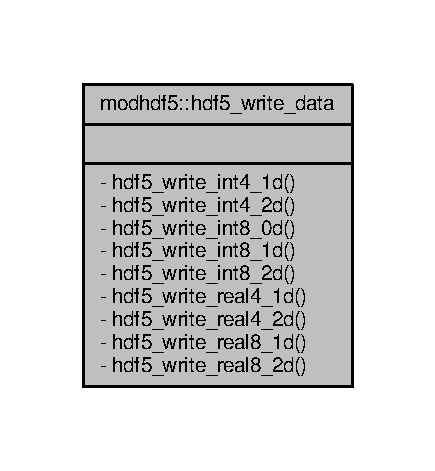
\includegraphics[width=209pt]{interfacemodhdf5_1_1hdf5__write__data__coll__graph}
\end{center}
\end{figure}
\subsection*{Private Member Functions}
\begin{DoxyCompactItemize}
\item 
subroutine \hyperlink{interfacemodhdf5_1_1hdf5__write__data_a33e6b35760f15f06a5804cd0caa3da0b}{hdf5\+\_\+write\+\_\+int4\+\_\+1d} (id, name, n1, data)
\begin{DoxyCompactList}\small\item\em Write a 1-\/D integer(kind=4) array in a serial file. \end{DoxyCompactList}\item 
subroutine \hyperlink{interfacemodhdf5_1_1hdf5__write__data_a3c4d3b976cc7ded0445f44f4806119eb}{hdf5\+\_\+write\+\_\+int4\+\_\+2d} (id, name, n1, n2, data)
\begin{DoxyCompactList}\small\item\em Write a 2-\/D integer(kind=4) array in a serial file. \end{DoxyCompactList}\item 
subroutine \hyperlink{interfacemodhdf5_1_1hdf5__write__data_a3d54b82d734756ac3b7e04eefa3f42b3}{hdf5\+\_\+write\+\_\+int8\+\_\+0d} (id, name, data)
\begin{DoxyCompactList}\small\item\em Write an integer(kind=8) scalar in a serial file. \end{DoxyCompactList}\item 
subroutine \hyperlink{interfacemodhdf5_1_1hdf5__write__data_ace548f4140d1a7c171dfa972edaae0ac}{hdf5\+\_\+write\+\_\+int8\+\_\+1d} (id, name, n1, data)
\begin{DoxyCompactList}\small\item\em Write a 1-\/D integer(kind=8) array in a serial file. \end{DoxyCompactList}\item 
subroutine \hyperlink{interfacemodhdf5_1_1hdf5__write__data_aeb5d82f4adffdf6967fde4ab3844674b}{hdf5\+\_\+write\+\_\+int8\+\_\+2d} (id, name, n1, n2, data)
\begin{DoxyCompactList}\small\item\em Write a 2-\/D integer(kind=8) array in a serial file. \end{DoxyCompactList}\item 
subroutine \hyperlink{interfacemodhdf5_1_1hdf5__write__data_a75929560447e383a91b35d46c4ce8914}{hdf5\+\_\+write\+\_\+real4\+\_\+1d} (id, name, n1, data)
\begin{DoxyCompactList}\small\item\em Write a 1-\/D real(kind=4) array in a serial file. \end{DoxyCompactList}\item 
subroutine \hyperlink{interfacemodhdf5_1_1hdf5__write__data_a62e0df9e9de4d8ef46e07a947aad26bc}{hdf5\+\_\+write\+\_\+real4\+\_\+2d} (id, name, n1, n2, data)
\begin{DoxyCompactList}\small\item\em Write a 2-\/D real(kind=4) array in a serial file. \end{DoxyCompactList}\item 
subroutine \hyperlink{interfacemodhdf5_1_1hdf5__write__data_aff5fc1508bad5874650807a0cad4a98d}{hdf5\+\_\+write\+\_\+real8\+\_\+1d} (id, name, n1, data)
\begin{DoxyCompactList}\small\item\em Write a 1-\/D real(kind=8) array in a serial file. \end{DoxyCompactList}\item 
subroutine \hyperlink{interfacemodhdf5_1_1hdf5__write__data_a8a1aae59f80f0cd54e7d32a0e564020f}{hdf5\+\_\+write\+\_\+real8\+\_\+2d} (id, name, n1, n2, data)
\begin{DoxyCompactList}\small\item\em Write a 2-\/D real(kind=8) array in a serial file. \end{DoxyCompactList}\end{DoxyCompactItemize}


\subsection{Detailed Description}
Generic inteface used to write data in a hdf5 file. 


\begin{DoxyParams}[1]{Parameters}
\mbox{\tt in}  & {\em id} & id of the file/group where the dataset will be written \\
\hline
\mbox{\tt in}  & {\em name} & name of the dataset \\
\hline
\mbox{\tt in}  & {\em n1} & first dimension of the data array \\
\hline
\mbox{\tt in}  & {\em n2} & second dimension of the data array (optional) \\
\hline
\mbox{\tt in}  & {\em data} & 1-\/D or 2-\/D data array of type Integer(4), Integer(8), Real(4) or Real(8) \\
\hline
\end{DoxyParams}


Definition at line 88 of file modhdf5.\+f90.



\subsection{Member Function/\+Subroutine Documentation}
\index{modhdf5\+::hdf5\+\_\+write\+\_\+data@{modhdf5\+::hdf5\+\_\+write\+\_\+data}!hdf5\+\_\+write\+\_\+int4\+\_\+1d@{hdf5\+\_\+write\+\_\+int4\+\_\+1d}}
\index{hdf5\+\_\+write\+\_\+int4\+\_\+1d@{hdf5\+\_\+write\+\_\+int4\+\_\+1d}!modhdf5\+::hdf5\+\_\+write\+\_\+data@{modhdf5\+::hdf5\+\_\+write\+\_\+data}}
\subsubsection[{\texorpdfstring{hdf5\+\_\+write\+\_\+int4\+\_\+1d(id, name, n1, data)}{hdf5_write_int4_1d(id, name, n1, data)}}]{\setlength{\rightskip}{0pt plus 5cm}subroutine modhdf5\+::hdf5\+\_\+write\+\_\+data\+::hdf5\+\_\+write\+\_\+int4\+\_\+1d (
\begin{DoxyParamCaption}
\item[{integer(hid\+\_\+t), intent(in)}]{id, }
\item[{character(len={\bf h5strlen}), intent(in)}]{name, }
\item[{integer, intent(in)}]{n1, }
\item[{integer(kind=4), dimension(n1), intent(in), target}]{data}
\end{DoxyParamCaption}
)\hspace{0.3cm}{\ttfamily [private]}}\hypertarget{interfacemodhdf5_1_1hdf5__write__data_a33e6b35760f15f06a5804cd0caa3da0b}{}\label{interfacemodhdf5_1_1hdf5__write__data_a33e6b35760f15f06a5804cd0caa3da0b}


Write a 1-\/D integer(kind=4) array in a serial file. 


\begin{DoxyParams}[1]{Parameters}
\mbox{\tt in}  & {\em id} & id of the file/group where the dataset will be written\\
\hline
\mbox{\tt in}  & {\em name} & name of the dataset\\
\hline
\mbox{\tt in}  & {\em n1} & dimension of the data\\
\hline
\mbox{\tt in}  & {\em data} & data array \\
\hline
\end{DoxyParams}


Definition at line 542 of file modhdf5.\+f90.

\index{modhdf5\+::hdf5\+\_\+write\+\_\+data@{modhdf5\+::hdf5\+\_\+write\+\_\+data}!hdf5\+\_\+write\+\_\+int4\+\_\+2d@{hdf5\+\_\+write\+\_\+int4\+\_\+2d}}
\index{hdf5\+\_\+write\+\_\+int4\+\_\+2d@{hdf5\+\_\+write\+\_\+int4\+\_\+2d}!modhdf5\+::hdf5\+\_\+write\+\_\+data@{modhdf5\+::hdf5\+\_\+write\+\_\+data}}
\subsubsection[{\texorpdfstring{hdf5\+\_\+write\+\_\+int4\+\_\+2d(id, name, n1, n2, data)}{hdf5_write_int4_2d(id, name, n1, n2, data)}}]{\setlength{\rightskip}{0pt plus 5cm}subroutine modhdf5\+::hdf5\+\_\+write\+\_\+data\+::hdf5\+\_\+write\+\_\+int4\+\_\+2d (
\begin{DoxyParamCaption}
\item[{integer(hid\+\_\+t), intent(in)}]{id, }
\item[{character(len={\bf h5strlen}), intent(in)}]{name, }
\item[{integer, intent(in)}]{n1, }
\item[{integer, intent(in)}]{n2, }
\item[{integer(kind=4), dimension(n1,n2), intent(in), target}]{data}
\end{DoxyParamCaption}
)\hspace{0.3cm}{\ttfamily [private]}}\hypertarget{interfacemodhdf5_1_1hdf5__write__data_a3c4d3b976cc7ded0445f44f4806119eb}{}\label{interfacemodhdf5_1_1hdf5__write__data_a3c4d3b976cc7ded0445f44f4806119eb}


Write a 2-\/D integer(kind=4) array in a serial file. 


\begin{DoxyParams}[1]{Parameters}
\mbox{\tt in}  & {\em id} & id of the file/group where the dataset will be written\\
\hline
\mbox{\tt in}  & {\em name} & name of the dataset\\
\hline
\mbox{\tt in}  & {\em n1} & first dimension of the data\\
\hline
\mbox{\tt in}  & {\em n2} & second dimension of the data\\
\hline
\mbox{\tt in}  & {\em data} & data array \\
\hline
\end{DoxyParams}


Definition at line 661 of file modhdf5.\+f90.

\index{modhdf5\+::hdf5\+\_\+write\+\_\+data@{modhdf5\+::hdf5\+\_\+write\+\_\+data}!hdf5\+\_\+write\+\_\+int8\+\_\+0d@{hdf5\+\_\+write\+\_\+int8\+\_\+0d}}
\index{hdf5\+\_\+write\+\_\+int8\+\_\+0d@{hdf5\+\_\+write\+\_\+int8\+\_\+0d}!modhdf5\+::hdf5\+\_\+write\+\_\+data@{modhdf5\+::hdf5\+\_\+write\+\_\+data}}
\subsubsection[{\texorpdfstring{hdf5\+\_\+write\+\_\+int8\+\_\+0d(id, name, data)}{hdf5_write_int8_0d(id, name, data)}}]{\setlength{\rightskip}{0pt plus 5cm}subroutine modhdf5\+::hdf5\+\_\+write\+\_\+data\+::hdf5\+\_\+write\+\_\+int8\+\_\+0d (
\begin{DoxyParamCaption}
\item[{integer(hid\+\_\+t), intent(in)}]{id, }
\item[{character(len={\bf h5strlen}), intent(in)}]{name, }
\item[{integer(kind=8), intent(in), target}]{data}
\end{DoxyParamCaption}
)\hspace{0.3cm}{\ttfamily [private]}}\hypertarget{interfacemodhdf5_1_1hdf5__write__data_a3d54b82d734756ac3b7e04eefa3f42b3}{}\label{interfacemodhdf5_1_1hdf5__write__data_a3d54b82d734756ac3b7e04eefa3f42b3}


Write an integer(kind=8) scalar in a serial file. 


\begin{DoxyParams}[1]{Parameters}
\mbox{\tt in}  & {\em id} & id of the file/group where the dataset will be written\\
\hline
\mbox{\tt in}  & {\em name} & name of the dataset\\
\hline
\mbox{\tt in}  & {\em data} & data scalar \\
\hline
\end{DoxyParams}


Definition at line 582 of file modhdf5.\+f90.

\index{modhdf5\+::hdf5\+\_\+write\+\_\+data@{modhdf5\+::hdf5\+\_\+write\+\_\+data}!hdf5\+\_\+write\+\_\+int8\+\_\+1d@{hdf5\+\_\+write\+\_\+int8\+\_\+1d}}
\index{hdf5\+\_\+write\+\_\+int8\+\_\+1d@{hdf5\+\_\+write\+\_\+int8\+\_\+1d}!modhdf5\+::hdf5\+\_\+write\+\_\+data@{modhdf5\+::hdf5\+\_\+write\+\_\+data}}
\subsubsection[{\texorpdfstring{hdf5\+\_\+write\+\_\+int8\+\_\+1d(id, name, n1, data)}{hdf5_write_int8_1d(id, name, n1, data)}}]{\setlength{\rightskip}{0pt plus 5cm}subroutine modhdf5\+::hdf5\+\_\+write\+\_\+data\+::hdf5\+\_\+write\+\_\+int8\+\_\+1d (
\begin{DoxyParamCaption}
\item[{integer(hid\+\_\+t), intent(in)}]{id, }
\item[{character(len={\bf h5strlen}), intent(in)}]{name, }
\item[{integer, intent(in)}]{n1, }
\item[{integer(kind=8), dimension(n1), intent(in), target}]{data}
\end{DoxyParamCaption}
)\hspace{0.3cm}{\ttfamily [private]}}\hypertarget{interfacemodhdf5_1_1hdf5__write__data_ace548f4140d1a7c171dfa972edaae0ac}{}\label{interfacemodhdf5_1_1hdf5__write__data_ace548f4140d1a7c171dfa972edaae0ac}


Write a 1-\/D integer(kind=8) array in a serial file. 


\begin{DoxyParams}[1]{Parameters}
\mbox{\tt in}  & {\em id} & id of the file/group where the dataset will be written\\
\hline
\mbox{\tt in}  & {\em name} & name of the dataset\\
\hline
\mbox{\tt in}  & {\em n1} & dimension of the data\\
\hline
\mbox{\tt in}  & {\em data} & data array \\
\hline
\end{DoxyParams}


Definition at line 621 of file modhdf5.\+f90.

\index{modhdf5\+::hdf5\+\_\+write\+\_\+data@{modhdf5\+::hdf5\+\_\+write\+\_\+data}!hdf5\+\_\+write\+\_\+int8\+\_\+2d@{hdf5\+\_\+write\+\_\+int8\+\_\+2d}}
\index{hdf5\+\_\+write\+\_\+int8\+\_\+2d@{hdf5\+\_\+write\+\_\+int8\+\_\+2d}!modhdf5\+::hdf5\+\_\+write\+\_\+data@{modhdf5\+::hdf5\+\_\+write\+\_\+data}}
\subsubsection[{\texorpdfstring{hdf5\+\_\+write\+\_\+int8\+\_\+2d(id, name, n1, n2, data)}{hdf5_write_int8_2d(id, name, n1, n2, data)}}]{\setlength{\rightskip}{0pt plus 5cm}subroutine modhdf5\+::hdf5\+\_\+write\+\_\+data\+::hdf5\+\_\+write\+\_\+int8\+\_\+2d (
\begin{DoxyParamCaption}
\item[{integer(hid\+\_\+t), intent(in)}]{id, }
\item[{character(len={\bf h5strlen}), intent(in)}]{name, }
\item[{integer, intent(in)}]{n1, }
\item[{integer, intent(in)}]{n2, }
\item[{integer(kind=8), dimension(n1,n2), intent(in), target}]{data}
\end{DoxyParamCaption}
)\hspace{0.3cm}{\ttfamily [private]}}\hypertarget{interfacemodhdf5_1_1hdf5__write__data_aeb5d82f4adffdf6967fde4ab3844674b}{}\label{interfacemodhdf5_1_1hdf5__write__data_aeb5d82f4adffdf6967fde4ab3844674b}


Write a 2-\/D integer(kind=8) array in a serial file. 


\begin{DoxyParams}[1]{Parameters}
\mbox{\tt in}  & {\em id} & id of the file/group where the dataset will be written\\
\hline
\mbox{\tt in}  & {\em name} & name of the dataset\\
\hline
\mbox{\tt in}  & {\em n1} & first dimension of the data\\
\hline
\mbox{\tt in}  & {\em n2} & second dimension of the data\\
\hline
\mbox{\tt in}  & {\em data} & data array \\
\hline
\end{DoxyParams}


Definition at line 703 of file modhdf5.\+f90.

\index{modhdf5\+::hdf5\+\_\+write\+\_\+data@{modhdf5\+::hdf5\+\_\+write\+\_\+data}!hdf5\+\_\+write\+\_\+real4\+\_\+1d@{hdf5\+\_\+write\+\_\+real4\+\_\+1d}}
\index{hdf5\+\_\+write\+\_\+real4\+\_\+1d@{hdf5\+\_\+write\+\_\+real4\+\_\+1d}!modhdf5\+::hdf5\+\_\+write\+\_\+data@{modhdf5\+::hdf5\+\_\+write\+\_\+data}}
\subsubsection[{\texorpdfstring{hdf5\+\_\+write\+\_\+real4\+\_\+1d(id, name, n1, data)}{hdf5_write_real4_1d(id, name, n1, data)}}]{\setlength{\rightskip}{0pt plus 5cm}subroutine modhdf5\+::hdf5\+\_\+write\+\_\+data\+::hdf5\+\_\+write\+\_\+real4\+\_\+1d (
\begin{DoxyParamCaption}
\item[{integer(hid\+\_\+t), intent(in)}]{id, }
\item[{character(len={\bf h5strlen}), intent(in)}]{name, }
\item[{integer, intent(in)}]{n1, }
\item[{real(kind=4), dimension(n1), intent(in), target}]{data}
\end{DoxyParamCaption}
)\hspace{0.3cm}{\ttfamily [private]}}\hypertarget{interfacemodhdf5_1_1hdf5__write__data_a75929560447e383a91b35d46c4ce8914}{}\label{interfacemodhdf5_1_1hdf5__write__data_a75929560447e383a91b35d46c4ce8914}


Write a 1-\/D real(kind=4) array in a serial file. 


\begin{DoxyParams}[1]{Parameters}
\mbox{\tt in}  & {\em id} & id of the file/group where the dataset will be written\\
\hline
\mbox{\tt in}  & {\em name} & name of the dataset\\
\hline
\mbox{\tt in}  & {\em n1} & dimension of the data\\
\hline
\mbox{\tt in}  & {\em data} & data array \\
\hline
\end{DoxyParams}


Definition at line 745 of file modhdf5.\+f90.

\index{modhdf5\+::hdf5\+\_\+write\+\_\+data@{modhdf5\+::hdf5\+\_\+write\+\_\+data}!hdf5\+\_\+write\+\_\+real4\+\_\+2d@{hdf5\+\_\+write\+\_\+real4\+\_\+2d}}
\index{hdf5\+\_\+write\+\_\+real4\+\_\+2d@{hdf5\+\_\+write\+\_\+real4\+\_\+2d}!modhdf5\+::hdf5\+\_\+write\+\_\+data@{modhdf5\+::hdf5\+\_\+write\+\_\+data}}
\subsubsection[{\texorpdfstring{hdf5\+\_\+write\+\_\+real4\+\_\+2d(id, name, n1, n2, data)}{hdf5_write_real4_2d(id, name, n1, n2, data)}}]{\setlength{\rightskip}{0pt plus 5cm}subroutine modhdf5\+::hdf5\+\_\+write\+\_\+data\+::hdf5\+\_\+write\+\_\+real4\+\_\+2d (
\begin{DoxyParamCaption}
\item[{integer(hid\+\_\+t), intent(in)}]{id, }
\item[{character(len={\bf h5strlen}), intent(in)}]{name, }
\item[{integer, intent(in)}]{n1, }
\item[{integer, intent(in)}]{n2, }
\item[{real(kind=4), dimension(n1,n2), intent(in), target}]{data}
\end{DoxyParamCaption}
)\hspace{0.3cm}{\ttfamily [private]}}\hypertarget{interfacemodhdf5_1_1hdf5__write__data_a62e0df9e9de4d8ef46e07a947aad26bc}{}\label{interfacemodhdf5_1_1hdf5__write__data_a62e0df9e9de4d8ef46e07a947aad26bc}


Write a 2-\/D real(kind=4) array in a serial file. 


\begin{DoxyParams}[1]{Parameters}
\mbox{\tt in}  & {\em id} & id of the file/group where the dataset will be written\\
\hline
\mbox{\tt in}  & {\em name} & name of the dataset\\
\hline
\mbox{\tt in}  & {\em n1} & first dimension of the data\\
\hline
\mbox{\tt in}  & {\em n2} & second dimension of the data\\
\hline
\mbox{\tt in}  & {\em data} & data array \\
\hline
\end{DoxyParams}


Definition at line 825 of file modhdf5.\+f90.

\index{modhdf5\+::hdf5\+\_\+write\+\_\+data@{modhdf5\+::hdf5\+\_\+write\+\_\+data}!hdf5\+\_\+write\+\_\+real8\+\_\+1d@{hdf5\+\_\+write\+\_\+real8\+\_\+1d}}
\index{hdf5\+\_\+write\+\_\+real8\+\_\+1d@{hdf5\+\_\+write\+\_\+real8\+\_\+1d}!modhdf5\+::hdf5\+\_\+write\+\_\+data@{modhdf5\+::hdf5\+\_\+write\+\_\+data}}
\subsubsection[{\texorpdfstring{hdf5\+\_\+write\+\_\+real8\+\_\+1d(id, name, n1, data)}{hdf5_write_real8_1d(id, name, n1, data)}}]{\setlength{\rightskip}{0pt plus 5cm}subroutine modhdf5\+::hdf5\+\_\+write\+\_\+data\+::hdf5\+\_\+write\+\_\+real8\+\_\+1d (
\begin{DoxyParamCaption}
\item[{integer(hid\+\_\+t), intent(in)}]{id, }
\item[{character(len={\bf h5strlen}), intent(in)}]{name, }
\item[{integer, intent(in)}]{n1, }
\item[{real(kind=8), dimension(n1), intent(in), target}]{data}
\end{DoxyParamCaption}
)\hspace{0.3cm}{\ttfamily [private]}}\hypertarget{interfacemodhdf5_1_1hdf5__write__data_aff5fc1508bad5874650807a0cad4a98d}{}\label{interfacemodhdf5_1_1hdf5__write__data_aff5fc1508bad5874650807a0cad4a98d}


Write a 1-\/D real(kind=8) array in a serial file. 


\begin{DoxyParams}[1]{Parameters}
\mbox{\tt in}  & {\em id} & id of the file/group where the dataset will be written\\
\hline
\mbox{\tt in}  & {\em name} & name of the dataset\\
\hline
\mbox{\tt in}  & {\em n1} & dimension of the data\\
\hline
\mbox{\tt in}  & {\em data} & data array \\
\hline
\end{DoxyParams}


Definition at line 785 of file modhdf5.\+f90.

\index{modhdf5\+::hdf5\+\_\+write\+\_\+data@{modhdf5\+::hdf5\+\_\+write\+\_\+data}!hdf5\+\_\+write\+\_\+real8\+\_\+2d@{hdf5\+\_\+write\+\_\+real8\+\_\+2d}}
\index{hdf5\+\_\+write\+\_\+real8\+\_\+2d@{hdf5\+\_\+write\+\_\+real8\+\_\+2d}!modhdf5\+::hdf5\+\_\+write\+\_\+data@{modhdf5\+::hdf5\+\_\+write\+\_\+data}}
\subsubsection[{\texorpdfstring{hdf5\+\_\+write\+\_\+real8\+\_\+2d(id, name, n1, n2, data)}{hdf5_write_real8_2d(id, name, n1, n2, data)}}]{\setlength{\rightskip}{0pt plus 5cm}subroutine modhdf5\+::hdf5\+\_\+write\+\_\+data\+::hdf5\+\_\+write\+\_\+real8\+\_\+2d (
\begin{DoxyParamCaption}
\item[{integer(hid\+\_\+t), intent(in)}]{id, }
\item[{character(len={\bf h5strlen}), intent(in)}]{name, }
\item[{integer, intent(in)}]{n1, }
\item[{integer, intent(in)}]{n2, }
\item[{real(kind=8), dimension(n1,n2), intent(in), target}]{data}
\end{DoxyParamCaption}
)\hspace{0.3cm}{\ttfamily [private]}}\hypertarget{interfacemodhdf5_1_1hdf5__write__data_a8a1aae59f80f0cd54e7d32a0e564020f}{}\label{interfacemodhdf5_1_1hdf5__write__data_a8a1aae59f80f0cd54e7d32a0e564020f}


Write a 2-\/D real(kind=8) array in a serial file. 


\begin{DoxyParams}[1]{Parameters}
\mbox{\tt in}  & {\em id} & id of the file/group where the dataset will be written\\
\hline
\mbox{\tt in}  & {\em name} & name of the dataset\\
\hline
\mbox{\tt in}  & {\em n1} & first dimension of the data\\
\hline
\mbox{\tt in}  & {\em n2} & second dimension of the data\\
\hline
\mbox{\tt in}  & {\em data} & data array \\
\hline
\end{DoxyParams}


Definition at line 867 of file modhdf5.\+f90.



The documentation for this interface was generated from the following file\+:\begin{DoxyCompactItemize}
\item 
/home/roy/\+Travail/\+Devel/\+Cosmologie/\+Pfof/trunk/common/src/\hyperlink{modhdf5_8f90}{modhdf5.\+f90}\end{DoxyCompactItemize}

\hypertarget{interfacemodhdf5_1_1hdf5__write__mpi__data}{\section{modhdf5\-:\-:hdf5\-\_\-write\-\_\-mpi\-\_\-data Interface Reference}
\label{interfacemodhdf5_1_1hdf5__write__mpi__data}\index{modhdf5\-::hdf5\-\_\-write\-\_\-mpi\-\_\-data@{modhdf5\-::hdf5\-\_\-write\-\_\-mpi\-\_\-data}}
}


Generic inteface used to write data in a parallel hdf5 file.  


\subsection*{Private Member Functions}
\begin{DoxyCompactItemize}
\item 
subroutine \hyperlink{interfacemodhdf5_1_1hdf5__write__mpi__data_a7ea09115ff2a974a7d871c555b1be2d0}{hdf5\-\_\-write\-\_\-mpi\-\_\-int4\-\_\-1d} (id, name, n1, data, comm, empty)
\begin{DoxyCompactList}\small\item\em Write a 1-\/\-D integer(kind=4) array in a parallel file. \end{DoxyCompactList}\item 
subroutine \hyperlink{interfacemodhdf5_1_1hdf5__write__mpi__data_a2906d576070456a5137a6e0abe667156}{hdf5\-\_\-write\-\_\-mpi\-\_\-int4\-\_\-2d} (id, name, n1, n2, data, comm, empty)
\begin{DoxyCompactList}\small\item\em Write a 2-\/\-D integer(kind=4) array in a parallel file The array is distributed along the 2nd dimension. \end{DoxyCompactList}\item 
subroutine \hyperlink{interfacemodhdf5_1_1hdf5__write__mpi__data_a9e1ae706eda63ff5c0be30ee69ec560a}{hdf5\-\_\-write\-\_\-mpi\-\_\-int8\-\_\-1d} (id, name, n1, data, comm, empty)
\begin{DoxyCompactList}\small\item\em Write a 1-\/\-D integer(kind=8) array in a parallel file. \end{DoxyCompactList}\item 
subroutine \hyperlink{interfacemodhdf5_1_1hdf5__write__mpi__data_a16185b9e0e6ab2aaaff9c931f4554e3a}{hdf5\-\_\-write\-\_\-mpi\-\_\-int8\-\_\-2d} (id, name, n1, n2, data, comm, empty)
\begin{DoxyCompactList}\small\item\em Write a 2-\/\-D integer(kind=8) array in a parallel file The array is distributed along the 2nd dimension. \end{DoxyCompactList}\item 
subroutine \hyperlink{interfacemodhdf5_1_1hdf5__write__mpi__data_abbbc965c3da38a9f6ba1a37d18f1384a}{hdf5\-\_\-write\-\_\-mpi\-\_\-real4\-\_\-1d} (id, name, n1, data, comm, empty)
\begin{DoxyCompactList}\small\item\em Write a 1-\/\-D real(kind=4) array in a parallel file. \end{DoxyCompactList}\item 
subroutine \hyperlink{interfacemodhdf5_1_1hdf5__write__mpi__data_a524aa3c194952012883099ad1b29df82}{hdf5\-\_\-write\-\_\-mpi\-\_\-real4\-\_\-2d} (id, name, n1, n2, data, comm, empty)
\begin{DoxyCompactList}\small\item\em Write a 2-\/\-D real(kind=4) array in a parallel file The array is distributed along the 2nd dimension. \end{DoxyCompactList}\item 
subroutine \hyperlink{interfacemodhdf5_1_1hdf5__write__mpi__data_ad323516e83fa60e25ecc34f7c6d5a21f}{hdf5\-\_\-write\-\_\-mpi\-\_\-real8\-\_\-1d} (id, name, n1, data, comm, empty)
\begin{DoxyCompactList}\small\item\em Write a 1-\/\-D real(kind=8) array in a parallel file. \end{DoxyCompactList}\item 
subroutine \hyperlink{interfacemodhdf5_1_1hdf5__write__mpi__data_ae7a2203ebd7ce2df80b58543f5afe1dc}{hdf5\-\_\-write\-\_\-mpi\-\_\-real8\-\_\-2d} (id, name, n1, n2, data, comm, empty)
\begin{DoxyCompactList}\small\item\em Write a 2-\/\-D real(kind=8) array in a parallel file The array is distributed along the 2nd dimension. \end{DoxyCompactList}\end{DoxyCompactItemize}


\subsection{Detailed Description}
Generic inteface used to write data in a parallel hdf5 file. 


\begin{DoxyParams}[1]{Parameters}
\mbox{\tt in}  & {\em id} & id of the file/group where the dataset will be written \\
\hline
\mbox{\tt in}  & {\em name} & name of the dataset \\
\hline
\mbox{\tt in}  & {\em n1} & first dimension of the data array \\
\hline
\mbox{\tt in}  & {\em n2} & second dimension of the data array (optional) \\
\hline
\mbox{\tt in}  & {\em data} & 1-\/\-D or 2-\/\-D data array of type Integer(4), Integer(8), Real(4) or Real(8) \\
\hline
\mbox{\tt in}  & {\em comm} & M\-P\-I communicator used for the output (the same communicator should have been used to create the file) \\
\hline
\end{DoxyParams}


Definition at line 125 of file modhdf5.\-f90.



\subsection{Member Function/\-Subroutine Documentation}
\hypertarget{interfacemodhdf5_1_1hdf5__write__mpi__data_a7ea09115ff2a974a7d871c555b1be2d0}{\index{modhdf5\-::hdf5\-\_\-write\-\_\-mpi\-\_\-data@{modhdf5\-::hdf5\-\_\-write\-\_\-mpi\-\_\-data}!hdf5\-\_\-write\-\_\-mpi\-\_\-int4\-\_\-1d@{hdf5\-\_\-write\-\_\-mpi\-\_\-int4\-\_\-1d}}
\index{hdf5\-\_\-write\-\_\-mpi\-\_\-int4\-\_\-1d@{hdf5\-\_\-write\-\_\-mpi\-\_\-int4\-\_\-1d}!modhdf5::hdf5_write_mpi_data@{modhdf5\-::hdf5\-\_\-write\-\_\-mpi\-\_\-data}}
\subsubsection[{hdf5\-\_\-write\-\_\-mpi\-\_\-int4\-\_\-1d}]{\setlength{\rightskip}{0pt plus 5cm}subroutine modhdf5\-::hdf5\-\_\-write\-\_\-mpi\-\_\-data\-::hdf5\-\_\-write\-\_\-mpi\-\_\-int4\-\_\-1d (
\begin{DoxyParamCaption}
\item[{integer(hid\-\_\-t), intent(in)}]{id, }
\item[{character(len={\bf h5strlen}), intent(in)}]{name, }
\item[{integer(kind=4), intent(in)}]{n1, }
\item[{integer(kind=4), dimension(n1), intent(in), target}]{data, }
\item[{integer(kind=4), intent(in)}]{comm, }
\item[{logical, intent(in), optional}]{empty}
\end{DoxyParamCaption}
)\hspace{0.3cm}{\ttfamily [private]}}}\label{interfacemodhdf5_1_1hdf5__write__mpi__data_a7ea09115ff2a974a7d871c555b1be2d0}


Write a 1-\/\-D integer(kind=4) array in a parallel file. 


\begin{DoxyParams}[1]{Parameters}
\mbox{\tt in}  & {\em id} & id of the file/group where the dataset will be written\\
\hline
\mbox{\tt in}  & {\em name} & name of the dataset\\
\hline
\mbox{\tt in}  & {\em n1} & dimension of the local data\\
\hline
\mbox{\tt in}  & {\em data} & local data array\\
\hline
\mbox{\tt in}  & {\em comm} & M\-P\-I communicator used \\
\hline
\end{DoxyParams}


Definition at line 913 of file modhdf5.\-f90.

\hypertarget{interfacemodhdf5_1_1hdf5__write__mpi__data_a2906d576070456a5137a6e0abe667156}{\index{modhdf5\-::hdf5\-\_\-write\-\_\-mpi\-\_\-data@{modhdf5\-::hdf5\-\_\-write\-\_\-mpi\-\_\-data}!hdf5\-\_\-write\-\_\-mpi\-\_\-int4\-\_\-2d@{hdf5\-\_\-write\-\_\-mpi\-\_\-int4\-\_\-2d}}
\index{hdf5\-\_\-write\-\_\-mpi\-\_\-int4\-\_\-2d@{hdf5\-\_\-write\-\_\-mpi\-\_\-int4\-\_\-2d}!modhdf5::hdf5_write_mpi_data@{modhdf5\-::hdf5\-\_\-write\-\_\-mpi\-\_\-data}}
\subsubsection[{hdf5\-\_\-write\-\_\-mpi\-\_\-int4\-\_\-2d}]{\setlength{\rightskip}{0pt plus 5cm}subroutine modhdf5\-::hdf5\-\_\-write\-\_\-mpi\-\_\-data\-::hdf5\-\_\-write\-\_\-mpi\-\_\-int4\-\_\-2d (
\begin{DoxyParamCaption}
\item[{integer(hid\-\_\-t), intent(in)}]{id, }
\item[{character(len={\bf h5strlen}), intent(in)}]{name, }
\item[{integer(kind=4), intent(in)}]{n1, }
\item[{integer(kind=4), intent(in)}]{n2, }
\item[{integer(kind=4), dimension(n1,n2), intent(in), target}]{data, }
\item[{integer(kind=4), intent(in)}]{comm, }
\item[{logical, intent(in), optional}]{empty}
\end{DoxyParamCaption}
)\hspace{0.3cm}{\ttfamily [private]}}}\label{interfacemodhdf5_1_1hdf5__write__mpi__data_a2906d576070456a5137a6e0abe667156}


Write a 2-\/\-D integer(kind=4) array in a parallel file The array is distributed along the 2nd dimension. 


\begin{DoxyParams}[1]{Parameters}
\mbox{\tt in}  & {\em id} & id of the file/group where the dataset will be written\\
\hline
\mbox{\tt in}  & {\em name} & name of the dataset\\
\hline
\mbox{\tt in}  & {\em n1} & first dimension of the local data\\
\hline
\mbox{\tt in}  & {\em n2} & second dimension of the local data\\
\hline
\mbox{\tt in}  & {\em data} & local data array\\
\hline
\mbox{\tt in}  & {\em comm} & M\-P\-I communicator used \\
\hline
\end{DoxyParams}


Definition at line 1010 of file modhdf5.\-f90.

\hypertarget{interfacemodhdf5_1_1hdf5__write__mpi__data_a9e1ae706eda63ff5c0be30ee69ec560a}{\index{modhdf5\-::hdf5\-\_\-write\-\_\-mpi\-\_\-data@{modhdf5\-::hdf5\-\_\-write\-\_\-mpi\-\_\-data}!hdf5\-\_\-write\-\_\-mpi\-\_\-int8\-\_\-1d@{hdf5\-\_\-write\-\_\-mpi\-\_\-int8\-\_\-1d}}
\index{hdf5\-\_\-write\-\_\-mpi\-\_\-int8\-\_\-1d@{hdf5\-\_\-write\-\_\-mpi\-\_\-int8\-\_\-1d}!modhdf5::hdf5_write_mpi_data@{modhdf5\-::hdf5\-\_\-write\-\_\-mpi\-\_\-data}}
\subsubsection[{hdf5\-\_\-write\-\_\-mpi\-\_\-int8\-\_\-1d}]{\setlength{\rightskip}{0pt plus 5cm}subroutine modhdf5\-::hdf5\-\_\-write\-\_\-mpi\-\_\-data\-::hdf5\-\_\-write\-\_\-mpi\-\_\-int8\-\_\-1d (
\begin{DoxyParamCaption}
\item[{integer(hid\-\_\-t), intent(in)}]{id, }
\item[{character(len={\bf h5strlen}), intent(in)}]{name, }
\item[{integer(kind=4), intent(in)}]{n1, }
\item[{integer(kind=8), dimension(n1), intent(in), target}]{data, }
\item[{integer(kind=4), intent(in)}]{comm, }
\item[{logical, intent(in), optional}]{empty}
\end{DoxyParamCaption}
)\hspace{0.3cm}{\ttfamily [private]}}}\label{interfacemodhdf5_1_1hdf5__write__mpi__data_a9e1ae706eda63ff5c0be30ee69ec560a}


Write a 1-\/\-D integer(kind=8) array in a parallel file. 


\begin{DoxyParams}[1]{Parameters}
\mbox{\tt in}  & {\em id} & id of the file/group where the dataset will be written\\
\hline
\mbox{\tt in}  & {\em name} & name of the dataset\\
\hline
\mbox{\tt in}  & {\em n1} & dimension of the local data\\
\hline
\mbox{\tt in}  & {\em data} & local data array\\
\hline
\mbox{\tt in}  & {\em comm} & M\-P\-I communicator used \\
\hline
\end{DoxyParams}


Definition at line 1111 of file modhdf5.\-f90.

\hypertarget{interfacemodhdf5_1_1hdf5__write__mpi__data_a16185b9e0e6ab2aaaff9c931f4554e3a}{\index{modhdf5\-::hdf5\-\_\-write\-\_\-mpi\-\_\-data@{modhdf5\-::hdf5\-\_\-write\-\_\-mpi\-\_\-data}!hdf5\-\_\-write\-\_\-mpi\-\_\-int8\-\_\-2d@{hdf5\-\_\-write\-\_\-mpi\-\_\-int8\-\_\-2d}}
\index{hdf5\-\_\-write\-\_\-mpi\-\_\-int8\-\_\-2d@{hdf5\-\_\-write\-\_\-mpi\-\_\-int8\-\_\-2d}!modhdf5::hdf5_write_mpi_data@{modhdf5\-::hdf5\-\_\-write\-\_\-mpi\-\_\-data}}
\subsubsection[{hdf5\-\_\-write\-\_\-mpi\-\_\-int8\-\_\-2d}]{\setlength{\rightskip}{0pt plus 5cm}subroutine modhdf5\-::hdf5\-\_\-write\-\_\-mpi\-\_\-data\-::hdf5\-\_\-write\-\_\-mpi\-\_\-int8\-\_\-2d (
\begin{DoxyParamCaption}
\item[{integer(hid\-\_\-t), intent(in)}]{id, }
\item[{character(len={\bf h5strlen}), intent(in)}]{name, }
\item[{integer(kind=4), intent(in)}]{n1, }
\item[{integer(kind=4), intent(in)}]{n2, }
\item[{integer(kind=8), dimension(n1,n2), intent(in), target}]{data, }
\item[{integer(kind=4), intent(in)}]{comm, }
\item[{logical, intent(in), optional}]{empty}
\end{DoxyParamCaption}
)\hspace{0.3cm}{\ttfamily [private]}}}\label{interfacemodhdf5_1_1hdf5__write__mpi__data_a16185b9e0e6ab2aaaff9c931f4554e3a}


Write a 2-\/\-D integer(kind=8) array in a parallel file The array is distributed along the 2nd dimension. 


\begin{DoxyParams}[1]{Parameters}
\mbox{\tt in}  & {\em id} & id of the file/group where the dataset will be written\\
\hline
\mbox{\tt in}  & {\em name} & name of the dataset\\
\hline
\mbox{\tt in}  & {\em n1} & first dimension of the local data\\
\hline
\mbox{\tt in}  & {\em n2} & second dimension of the local data\\
\hline
\mbox{\tt in}  & {\em data} & local data array\\
\hline
\mbox{\tt in}  & {\em comm} & M\-P\-I communicator used \\
\hline
\end{DoxyParams}


Definition at line 1218 of file modhdf5.\-f90.

\hypertarget{interfacemodhdf5_1_1hdf5__write__mpi__data_abbbc965c3da38a9f6ba1a37d18f1384a}{\index{modhdf5\-::hdf5\-\_\-write\-\_\-mpi\-\_\-data@{modhdf5\-::hdf5\-\_\-write\-\_\-mpi\-\_\-data}!hdf5\-\_\-write\-\_\-mpi\-\_\-real4\-\_\-1d@{hdf5\-\_\-write\-\_\-mpi\-\_\-real4\-\_\-1d}}
\index{hdf5\-\_\-write\-\_\-mpi\-\_\-real4\-\_\-1d@{hdf5\-\_\-write\-\_\-mpi\-\_\-real4\-\_\-1d}!modhdf5::hdf5_write_mpi_data@{modhdf5\-::hdf5\-\_\-write\-\_\-mpi\-\_\-data}}
\subsubsection[{hdf5\-\_\-write\-\_\-mpi\-\_\-real4\-\_\-1d}]{\setlength{\rightskip}{0pt plus 5cm}subroutine modhdf5\-::hdf5\-\_\-write\-\_\-mpi\-\_\-data\-::hdf5\-\_\-write\-\_\-mpi\-\_\-real4\-\_\-1d (
\begin{DoxyParamCaption}
\item[{integer(hid\-\_\-t), intent(in)}]{id, }
\item[{character(len={\bf h5strlen}), intent(in)}]{name, }
\item[{integer(kind=4), intent(in)}]{n1, }
\item[{real(kind=4), dimension(n1), intent(in), target}]{data, }
\item[{integer(kind=4), intent(in)}]{comm, }
\item[{logical, intent(in), optional}]{empty}
\end{DoxyParamCaption}
)\hspace{0.3cm}{\ttfamily [private]}}}\label{interfacemodhdf5_1_1hdf5__write__mpi__data_abbbc965c3da38a9f6ba1a37d18f1384a}


Write a 1-\/\-D real(kind=4) array in a parallel file. 


\begin{DoxyParams}[1]{Parameters}
\mbox{\tt in}  & {\em id} & id of the file/group where the dataset will be written\\
\hline
\mbox{\tt in}  & {\em name} & name of the dataset\\
\hline
\mbox{\tt in}  & {\em n1} & dimension of the local data\\
\hline
\mbox{\tt in}  & {\em data} & local data array\\
\hline
\mbox{\tt in}  & {\em comm} & M\-P\-I communicator used \\
\hline
\end{DoxyParams}


Definition at line 1319 of file modhdf5.\-f90.

\hypertarget{interfacemodhdf5_1_1hdf5__write__mpi__data_a524aa3c194952012883099ad1b29df82}{\index{modhdf5\-::hdf5\-\_\-write\-\_\-mpi\-\_\-data@{modhdf5\-::hdf5\-\_\-write\-\_\-mpi\-\_\-data}!hdf5\-\_\-write\-\_\-mpi\-\_\-real4\-\_\-2d@{hdf5\-\_\-write\-\_\-mpi\-\_\-real4\-\_\-2d}}
\index{hdf5\-\_\-write\-\_\-mpi\-\_\-real4\-\_\-2d@{hdf5\-\_\-write\-\_\-mpi\-\_\-real4\-\_\-2d}!modhdf5::hdf5_write_mpi_data@{modhdf5\-::hdf5\-\_\-write\-\_\-mpi\-\_\-data}}
\subsubsection[{hdf5\-\_\-write\-\_\-mpi\-\_\-real4\-\_\-2d}]{\setlength{\rightskip}{0pt plus 5cm}subroutine modhdf5\-::hdf5\-\_\-write\-\_\-mpi\-\_\-data\-::hdf5\-\_\-write\-\_\-mpi\-\_\-real4\-\_\-2d (
\begin{DoxyParamCaption}
\item[{integer(hid\-\_\-t), intent(in)}]{id, }
\item[{character(len={\bf h5strlen}), intent(in)}]{name, }
\item[{integer(kind=4), intent(in)}]{n1, }
\item[{integer(kind=4), intent(in)}]{n2, }
\item[{real(kind=4), dimension(n1,n2), intent(in), target}]{data, }
\item[{integer(kind=4), intent(in)}]{comm, }
\item[{logical, intent(in), optional}]{empty}
\end{DoxyParamCaption}
)\hspace{0.3cm}{\ttfamily [private]}}}\label{interfacemodhdf5_1_1hdf5__write__mpi__data_a524aa3c194952012883099ad1b29df82}


Write a 2-\/\-D real(kind=4) array in a parallel file The array is distributed along the 2nd dimension. 


\begin{DoxyParams}[1]{Parameters}
\mbox{\tt in}  & {\em id} & id of the file/group where the dataset will be written\\
\hline
\mbox{\tt in}  & {\em name} & name of the dataset\\
\hline
\mbox{\tt in}  & {\em n1} & first dimension of the local data\\
\hline
\mbox{\tt in}  & {\em n2} & second dimension of the local data\\
\hline
\mbox{\tt in}  & {\em data} & local data array\\
\hline
\mbox{\tt in}  & {\em comm} & M\-P\-I communicator used \\
\hline
\end{DoxyParams}


Definition at line 1417 of file modhdf5.\-f90.

\hypertarget{interfacemodhdf5_1_1hdf5__write__mpi__data_ad323516e83fa60e25ecc34f7c6d5a21f}{\index{modhdf5\-::hdf5\-\_\-write\-\_\-mpi\-\_\-data@{modhdf5\-::hdf5\-\_\-write\-\_\-mpi\-\_\-data}!hdf5\-\_\-write\-\_\-mpi\-\_\-real8\-\_\-1d@{hdf5\-\_\-write\-\_\-mpi\-\_\-real8\-\_\-1d}}
\index{hdf5\-\_\-write\-\_\-mpi\-\_\-real8\-\_\-1d@{hdf5\-\_\-write\-\_\-mpi\-\_\-real8\-\_\-1d}!modhdf5::hdf5_write_mpi_data@{modhdf5\-::hdf5\-\_\-write\-\_\-mpi\-\_\-data}}
\subsubsection[{hdf5\-\_\-write\-\_\-mpi\-\_\-real8\-\_\-1d}]{\setlength{\rightskip}{0pt plus 5cm}subroutine modhdf5\-::hdf5\-\_\-write\-\_\-mpi\-\_\-data\-::hdf5\-\_\-write\-\_\-mpi\-\_\-real8\-\_\-1d (
\begin{DoxyParamCaption}
\item[{integer(hid\-\_\-t), intent(in)}]{id, }
\item[{character(len={\bf h5strlen}), intent(in)}]{name, }
\item[{integer(kind=4), intent(in)}]{n1, }
\item[{real(kind=8), dimension(n1), intent(in), target}]{data, }
\item[{integer(kind=4), intent(in)}]{comm, }
\item[{logical, intent(in), optional}]{empty}
\end{DoxyParamCaption}
)\hspace{0.3cm}{\ttfamily [private]}}}\label{interfacemodhdf5_1_1hdf5__write__mpi__data_ad323516e83fa60e25ecc34f7c6d5a21f}


Write a 1-\/\-D real(kind=8) array in a parallel file. 


\begin{DoxyParams}[1]{Parameters}
\mbox{\tt in}  & {\em id} & id of the file/group where the dataset will be written\\
\hline
\mbox{\tt in}  & {\em name} & name of the dataset\\
\hline
\mbox{\tt in}  & {\em n1} & dimension of the local data\\
\hline
\mbox{\tt in}  & {\em data} & local data array\\
\hline
\mbox{\tt in}  & {\em comm} & M\-P\-I communicator used \\
\hline
\end{DoxyParams}


Definition at line 1527 of file modhdf5.\-f90.

\hypertarget{interfacemodhdf5_1_1hdf5__write__mpi__data_ae7a2203ebd7ce2df80b58543f5afe1dc}{\index{modhdf5\-::hdf5\-\_\-write\-\_\-mpi\-\_\-data@{modhdf5\-::hdf5\-\_\-write\-\_\-mpi\-\_\-data}!hdf5\-\_\-write\-\_\-mpi\-\_\-real8\-\_\-2d@{hdf5\-\_\-write\-\_\-mpi\-\_\-real8\-\_\-2d}}
\index{hdf5\-\_\-write\-\_\-mpi\-\_\-real8\-\_\-2d@{hdf5\-\_\-write\-\_\-mpi\-\_\-real8\-\_\-2d}!modhdf5::hdf5_write_mpi_data@{modhdf5\-::hdf5\-\_\-write\-\_\-mpi\-\_\-data}}
\subsubsection[{hdf5\-\_\-write\-\_\-mpi\-\_\-real8\-\_\-2d}]{\setlength{\rightskip}{0pt plus 5cm}subroutine modhdf5\-::hdf5\-\_\-write\-\_\-mpi\-\_\-data\-::hdf5\-\_\-write\-\_\-mpi\-\_\-real8\-\_\-2d (
\begin{DoxyParamCaption}
\item[{integer(hid\-\_\-t), intent(in)}]{id, }
\item[{character(len={\bf h5strlen}), intent(in)}]{name, }
\item[{integer(kind=4), intent(in)}]{n1, }
\item[{integer(kind=4), intent(in)}]{n2, }
\item[{real(kind=8), dimension(n1,n2), intent(in), target}]{data, }
\item[{integer(kind=4), intent(in)}]{comm, }
\item[{logical, intent(in), optional}]{empty}
\end{DoxyParamCaption}
)\hspace{0.3cm}{\ttfamily [private]}}}\label{interfacemodhdf5_1_1hdf5__write__mpi__data_ae7a2203ebd7ce2df80b58543f5afe1dc}


Write a 2-\/\-D real(kind=8) array in a parallel file The array is distributed along the 2nd dimension. 


\begin{DoxyParams}[1]{Parameters}
\mbox{\tt in}  & {\em id} & id of the file/group where the dataset will be written\\
\hline
\mbox{\tt in}  & {\em name} & name of the dataset\\
\hline
\mbox{\tt in}  & {\em n1} & first dimension of the local data\\
\hline
\mbox{\tt in}  & {\em n2} & second dimension of the local data\\
\hline
\mbox{\tt in}  & {\em data} & local data array\\
\hline
\mbox{\tt in}  & {\em comm} & M\-P\-I communicator used \\
\hline
\end{DoxyParams}


Definition at line 1625 of file modhdf5.\-f90.



The documentation for this interface was generated from the following file\-:\begin{DoxyCompactItemize}
\item 
/home/roy/\-Travail/\-Devel/\-Cosmologie/\-Pfof/branches/\-Modif\-Struct/common/src/\hyperlink{modhdf5_8f90}{modhdf5.\-f90}\end{DoxyCompactItemize}

\hypertarget{interfacemodsortinterf_1_1heapsort}{}\section{modsortinterf\+:\+:heapsort Interface Reference}
\label{interfacemodsortinterf_1_1heapsort}\index{modsortinterf\+::heapsort@{modsortinterf\+::heapsort}}


Collaboration diagram for modsortinterf\+:\+:heapsort\+:\nopagebreak
\begin{figure}[H]
\begin{center}
\leavevmode
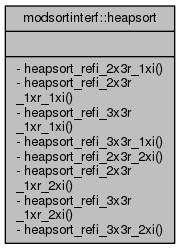
\includegraphics[width=207pt]{interfacemodsortinterf_1_1heapsort__coll__graph}
\end{center}
\end{figure}
\subsection*{Private Member Functions}
\begin{DoxyCompactItemize}
\item 
subroutine \hyperlink{interfacemodsortinterf_1_1heapsort_a5cbbb5add647e60a3338d4d5aa5bc0c4}{heapsort\+\_\+refi\+\_\+2x3r\+\_\+1xi} (n, tref, tx, tv, tid)
\item 
subroutine \hyperlink{interfacemodsortinterf_1_1heapsort_acf802a187b3156217c5189914fc3c5dc}{heapsort\+\_\+refi\+\_\+2x3r\+\_\+1xr\+\_\+1xi} (n, tref, tx, tv, tp, tid)
\begin{DoxyCompactList}\small\item\em Heap sort as described in Introduction to algorithms (Cormen, Leiserson, Rivest, Stein) \end{DoxyCompactList}\item 
subroutine \hyperlink{interfacemodsortinterf_1_1heapsort_a1b0496cffffd026ecd963c6c940f74c1}{heapsort\+\_\+refi\+\_\+3x3r\+\_\+1xr\+\_\+1xi} (n, tref, tx, tv, tf, tp, tid)
\item 
subroutine \hyperlink{interfacemodsortinterf_1_1heapsort_a0ba1556a756726e4b7f9339970f089b1}{heapsort\+\_\+refi\+\_\+3x3r\+\_\+1xi} (n, tref, tx, tv, tf, tid)
\item 
subroutine \hyperlink{interfacemodsortinterf_1_1heapsort_a2660aea691c9178df3aa11af9a6cc8f3}{heapsort\+\_\+refi\+\_\+2x3r\+\_\+2xi} (n, tref, tx, tv, tid, trid)
\item 
subroutine \hyperlink{interfacemodsortinterf_1_1heapsort_a495a6f6342a96d0bc2c5fcb731f0dd2f}{heapsort\+\_\+refi\+\_\+2x3r\+\_\+1xr\+\_\+2xi} (n, tref, tx, tv, tp, tid, trid)
\item 
subroutine \hyperlink{interfacemodsortinterf_1_1heapsort_a002758c8edf00e36596148059c845a3b}{heapsort\+\_\+refi\+\_\+3x3r\+\_\+1xr\+\_\+2xi} (n, tref, tx, tv, tf, tp, tid, trid)
\item 
subroutine \hyperlink{interfacemodsortinterf_1_1heapsort_a10a0ffdd549dc88c7787c43899c321b0}{heapsort\+\_\+refi\+\_\+3x3r\+\_\+2xi} (n, tref, tx, tv, tf, tid, trid)
\end{DoxyCompactItemize}


\subsection{Detailed Description}


Definition at line 21 of file modsortinterf.\+f90.



\subsection{Member Function/\+Subroutine Documentation}
\index{modsortinterf\+::heapsort@{modsortinterf\+::heapsort}!heapsort\+\_\+refi\+\_\+2x3r\+\_\+1xi@{heapsort\+\_\+refi\+\_\+2x3r\+\_\+1xi}}
\index{heapsort\+\_\+refi\+\_\+2x3r\+\_\+1xi@{heapsort\+\_\+refi\+\_\+2x3r\+\_\+1xi}!modsortinterf\+::heapsort@{modsortinterf\+::heapsort}}
\subsubsection[{\texorpdfstring{heapsort\+\_\+refi\+\_\+2x3r\+\_\+1xi(n, tref, tx, tv, tid)}{heapsort_refi_2x3r_1xi(n, tref, tx, tv, tid)}}]{\setlength{\rightskip}{0pt plus 5cm}subroutine modsortinterf\+::heapsort\+::heapsort\+\_\+refi\+\_\+2x3r\+\_\+1xi (
\begin{DoxyParamCaption}
\item[{integer(kind=4), intent(in)}]{n, }
\item[{integer(kind=pri), dimension($\ast$), intent(inout)}]{tref, }
\item[{real (kind=4), dimension(3,$\ast$), intent(inout)}]{tx, }
\item[{real (kind=4), dimension(3,$\ast$), intent(inout)}]{tv, }
\item[{integer(kind=pri), dimension($\ast$), intent(inout)}]{tid}
\end{DoxyParamCaption}
)\hspace{0.3cm}{\ttfamily [private]}}\hypertarget{interfacemodsortinterf_1_1heapsort_a5cbbb5add647e60a3338d4d5aa5bc0c4}{}\label{interfacemodsortinterf_1_1heapsort_a5cbbb5add647e60a3338d4d5aa5bc0c4}


Definition at line 651 of file modsortinterf.\+f90.

\index{modsortinterf\+::heapsort@{modsortinterf\+::heapsort}!heapsort\+\_\+refi\+\_\+2x3r\+\_\+1xr\+\_\+1xi@{heapsort\+\_\+refi\+\_\+2x3r\+\_\+1xr\+\_\+1xi}}
\index{heapsort\+\_\+refi\+\_\+2x3r\+\_\+1xr\+\_\+1xi@{heapsort\+\_\+refi\+\_\+2x3r\+\_\+1xr\+\_\+1xi}!modsortinterf\+::heapsort@{modsortinterf\+::heapsort}}
\subsubsection[{\texorpdfstring{heapsort\+\_\+refi\+\_\+2x3r\+\_\+1xr\+\_\+1xi(n, tref, tx, tv, tp, tid)}{heapsort_refi_2x3r_1xr_1xi(n, tref, tx, tv, tp, tid)}}]{\setlength{\rightskip}{0pt plus 5cm}subroutine modsortinterf\+::heapsort\+::heapsort\+\_\+refi\+\_\+2x3r\+\_\+1xr\+\_\+1xi (
\begin{DoxyParamCaption}
\item[{integer(kind=4), intent(in)}]{n, }
\item[{integer(kind=pri), dimension($\ast$), intent(inout)}]{tref, }
\item[{real (kind=4), dimension(3,$\ast$), intent(inout)}]{tx, }
\item[{real (kind=4), dimension(3,$\ast$), intent(inout)}]{tv, }
\item[{real (kind=4), dimension($\ast$), intent(inout)}]{tp, }
\item[{integer(kind=pri), dimension($\ast$), intent(inout)}]{tid}
\end{DoxyParamCaption}
)\hspace{0.3cm}{\ttfamily [private]}}\hypertarget{interfacemodsortinterf_1_1heapsort_acf802a187b3156217c5189914fc3c5dc}{}\label{interfacemodsortinterf_1_1heapsort_acf802a187b3156217c5189914fc3c5dc}


Heap sort as described in Introduction to algorithms (Cormen, Leiserson, Rivest, Stein) 



Definition at line 479 of file modsortinterf.\+f90.

\index{modsortinterf\+::heapsort@{modsortinterf\+::heapsort}!heapsort\+\_\+refi\+\_\+2x3r\+\_\+1xr\+\_\+2xi@{heapsort\+\_\+refi\+\_\+2x3r\+\_\+1xr\+\_\+2xi}}
\index{heapsort\+\_\+refi\+\_\+2x3r\+\_\+1xr\+\_\+2xi@{heapsort\+\_\+refi\+\_\+2x3r\+\_\+1xr\+\_\+2xi}!modsortinterf\+::heapsort@{modsortinterf\+::heapsort}}
\subsubsection[{\texorpdfstring{heapsort\+\_\+refi\+\_\+2x3r\+\_\+1xr\+\_\+2xi(n, tref, tx, tv, tp, tid, trid)}{heapsort_refi_2x3r_1xr_2xi(n, tref, tx, tv, tp, tid, trid)}}]{\setlength{\rightskip}{0pt plus 5cm}subroutine modsortinterf\+::heapsort\+::heapsort\+\_\+refi\+\_\+2x3r\+\_\+1xr\+\_\+2xi (
\begin{DoxyParamCaption}
\item[{integer(kind=4), intent(in)}]{n, }
\item[{integer(kind=pri), dimension($\ast$), intent(inout)}]{tref, }
\item[{real (kind=4), dimension(3,$\ast$), intent(inout)}]{tx, }
\item[{real (kind=4), dimension(3,$\ast$), intent(inout)}]{tv, }
\item[{real (kind=4), dimension($\ast$), intent(inout)}]{tp, }
\item[{integer(kind=pri), dimension($\ast$), intent(inout)}]{tid, }
\item[{integer(kind=pri), dimension($\ast$), intent(inout)}]{trid}
\end{DoxyParamCaption}
)\hspace{0.3cm}{\ttfamily [private]}}\hypertarget{interfacemodsortinterf_1_1heapsort_a495a6f6342a96d0bc2c5fcb731f0dd2f}{}\label{interfacemodsortinterf_1_1heapsort_a495a6f6342a96d0bc2c5fcb731f0dd2f}


Definition at line 1182 of file modsortinterf.\+f90.

\index{modsortinterf\+::heapsort@{modsortinterf\+::heapsort}!heapsort\+\_\+refi\+\_\+2x3r\+\_\+2xi@{heapsort\+\_\+refi\+\_\+2x3r\+\_\+2xi}}
\index{heapsort\+\_\+refi\+\_\+2x3r\+\_\+2xi@{heapsort\+\_\+refi\+\_\+2x3r\+\_\+2xi}!modsortinterf\+::heapsort@{modsortinterf\+::heapsort}}
\subsubsection[{\texorpdfstring{heapsort\+\_\+refi\+\_\+2x3r\+\_\+2xi(n, tref, tx, tv, tid, trid)}{heapsort_refi_2x3r_2xi(n, tref, tx, tv, tid, trid)}}]{\setlength{\rightskip}{0pt plus 5cm}subroutine modsortinterf\+::heapsort\+::heapsort\+\_\+refi\+\_\+2x3r\+\_\+2xi (
\begin{DoxyParamCaption}
\item[{integer(kind=4), intent(in)}]{n, }
\item[{integer(kind=pri), dimension($\ast$), intent(inout)}]{tref, }
\item[{real (kind=4), dimension(3,$\ast$), intent(inout)}]{tx, }
\item[{real (kind=4), dimension(3,$\ast$), intent(inout)}]{tv, }
\item[{integer(kind=pri), dimension($\ast$), intent(inout)}]{tid, }
\item[{integer(kind=pri), dimension($\ast$), intent(inout)}]{trid}
\end{DoxyParamCaption}
)\hspace{0.3cm}{\ttfamily [private]}}\hypertarget{interfacemodsortinterf_1_1heapsort_a2660aea691c9178df3aa11af9a6cc8f3}{}\label{interfacemodsortinterf_1_1heapsort_a2660aea691c9178df3aa11af9a6cc8f3}


Definition at line 1358 of file modsortinterf.\+f90.

\index{modsortinterf\+::heapsort@{modsortinterf\+::heapsort}!heapsort\+\_\+refi\+\_\+3x3r\+\_\+1xi@{heapsort\+\_\+refi\+\_\+3x3r\+\_\+1xi}}
\index{heapsort\+\_\+refi\+\_\+3x3r\+\_\+1xi@{heapsort\+\_\+refi\+\_\+3x3r\+\_\+1xi}!modsortinterf\+::heapsort@{modsortinterf\+::heapsort}}
\subsubsection[{\texorpdfstring{heapsort\+\_\+refi\+\_\+3x3r\+\_\+1xi(n, tref, tx, tv, tf, tid)}{heapsort_refi_3x3r_1xi(n, tref, tx, tv, tf, tid)}}]{\setlength{\rightskip}{0pt plus 5cm}subroutine modsortinterf\+::heapsort\+::heapsort\+\_\+refi\+\_\+3x3r\+\_\+1xi (
\begin{DoxyParamCaption}
\item[{integer(kind=4), intent(in)}]{n, }
\item[{integer(kind=pri), dimension($\ast$), intent(inout)}]{tref, }
\item[{real (kind=4), dimension(3,$\ast$), intent(inout)}]{tx, }
\item[{real (kind=4), dimension(3,$\ast$), intent(inout)}]{tv, }
\item[{real (kind=4), dimension(3,$\ast$), intent(inout)}]{tf, }
\item[{integer(kind=pri), dimension($\ast$), intent(inout)}]{tid}
\end{DoxyParamCaption}
)\hspace{0.3cm}{\ttfamily [private]}}\hypertarget{interfacemodsortinterf_1_1heapsort_a0ba1556a756726e4b7f9339970f089b1}{}\label{interfacemodsortinterf_1_1heapsort_a0ba1556a756726e4b7f9339970f089b1}


Definition at line 988 of file modsortinterf.\+f90.

\index{modsortinterf\+::heapsort@{modsortinterf\+::heapsort}!heapsort\+\_\+refi\+\_\+3x3r\+\_\+1xr\+\_\+1xi@{heapsort\+\_\+refi\+\_\+3x3r\+\_\+1xr\+\_\+1xi}}
\index{heapsort\+\_\+refi\+\_\+3x3r\+\_\+1xr\+\_\+1xi@{heapsort\+\_\+refi\+\_\+3x3r\+\_\+1xr\+\_\+1xi}!modsortinterf\+::heapsort@{modsortinterf\+::heapsort}}
\subsubsection[{\texorpdfstring{heapsort\+\_\+refi\+\_\+3x3r\+\_\+1xr\+\_\+1xi(n, tref, tx, tv, tf, tp, tid)}{heapsort_refi_3x3r_1xr_1xi(n, tref, tx, tv, tf, tp, tid)}}]{\setlength{\rightskip}{0pt plus 5cm}subroutine modsortinterf\+::heapsort\+::heapsort\+\_\+refi\+\_\+3x3r\+\_\+1xr\+\_\+1xi (
\begin{DoxyParamCaption}
\item[{integer(kind=4), intent(in)}]{n, }
\item[{integer(kind=pri), dimension($\ast$), intent(inout)}]{tref, }
\item[{real (kind=4), dimension(3,$\ast$), intent(inout)}]{tx, }
\item[{real (kind=4), dimension(3,$\ast$), intent(inout)}]{tv, }
\item[{real (kind=4), dimension(3,$\ast$), intent(inout)}]{tf, }
\item[{real (kind=4), dimension($\ast$), intent(inout)}]{tp, }
\item[{integer(kind=pri), dimension($\ast$), intent(inout)}]{tid}
\end{DoxyParamCaption}
)\hspace{0.3cm}{\ttfamily [private]}}\hypertarget{interfacemodsortinterf_1_1heapsort_a1b0496cffffd026ecd963c6c940f74c1}{}\label{interfacemodsortinterf_1_1heapsort_a1b0496cffffd026ecd963c6c940f74c1}


Definition at line 810 of file modsortinterf.\+f90.

\index{modsortinterf\+::heapsort@{modsortinterf\+::heapsort}!heapsort\+\_\+refi\+\_\+3x3r\+\_\+1xr\+\_\+2xi@{heapsort\+\_\+refi\+\_\+3x3r\+\_\+1xr\+\_\+2xi}}
\index{heapsort\+\_\+refi\+\_\+3x3r\+\_\+1xr\+\_\+2xi@{heapsort\+\_\+refi\+\_\+3x3r\+\_\+1xr\+\_\+2xi}!modsortinterf\+::heapsort@{modsortinterf\+::heapsort}}
\subsubsection[{\texorpdfstring{heapsort\+\_\+refi\+\_\+3x3r\+\_\+1xr\+\_\+2xi(n, tref, tx, tv, tf, tp, tid, trid)}{heapsort_refi_3x3r_1xr_2xi(n, tref, tx, tv, tf, tp, tid, trid)}}]{\setlength{\rightskip}{0pt plus 5cm}subroutine modsortinterf\+::heapsort\+::heapsort\+\_\+refi\+\_\+3x3r\+\_\+1xr\+\_\+2xi (
\begin{DoxyParamCaption}
\item[{integer(kind=4), intent(in)}]{n, }
\item[{integer(kind=pri), dimension($\ast$), intent(inout)}]{tref, }
\item[{real (kind=4), dimension(3,$\ast$), intent(inout)}]{tx, }
\item[{real (kind=4), dimension(3,$\ast$), intent(inout)}]{tv, }
\item[{real (kind=4), dimension(3,$\ast$), intent(inout)}]{tf, }
\item[{real (kind=4), dimension($\ast$), intent(inout)}]{tp, }
\item[{integer(kind=pri), dimension($\ast$), intent(inout)}]{tid, }
\item[{integer(kind=pri), dimension($\ast$), intent(inout)}]{trid}
\end{DoxyParamCaption}
)\hspace{0.3cm}{\ttfamily [private]}}\hypertarget{interfacemodsortinterf_1_1heapsort_a002758c8edf00e36596148059c845a3b}{}\label{interfacemodsortinterf_1_1heapsort_a002758c8edf00e36596148059c845a3b}


Definition at line 1521 of file modsortinterf.\+f90.

\index{modsortinterf\+::heapsort@{modsortinterf\+::heapsort}!heapsort\+\_\+refi\+\_\+3x3r\+\_\+2xi@{heapsort\+\_\+refi\+\_\+3x3r\+\_\+2xi}}
\index{heapsort\+\_\+refi\+\_\+3x3r\+\_\+2xi@{heapsort\+\_\+refi\+\_\+3x3r\+\_\+2xi}!modsortinterf\+::heapsort@{modsortinterf\+::heapsort}}
\subsubsection[{\texorpdfstring{heapsort\+\_\+refi\+\_\+3x3r\+\_\+2xi(n, tref, tx, tv, tf, tid, trid)}{heapsort_refi_3x3r_2xi(n, tref, tx, tv, tf, tid, trid)}}]{\setlength{\rightskip}{0pt plus 5cm}subroutine modsortinterf\+::heapsort\+::heapsort\+\_\+refi\+\_\+3x3r\+\_\+2xi (
\begin{DoxyParamCaption}
\item[{integer(kind=4), intent(in)}]{n, }
\item[{integer(kind=pri), dimension($\ast$), intent(inout)}]{tref, }
\item[{real (kind=4), dimension(3,$\ast$), intent(inout)}]{tx, }
\item[{real (kind=4), dimension(3,$\ast$), intent(inout)}]{tv, }
\item[{real (kind=4), dimension(3,$\ast$), intent(inout)}]{tf, }
\item[{integer(kind=pri), dimension($\ast$), intent(inout)}]{tid, }
\item[{integer(kind=pri), dimension($\ast$), intent(inout)}]{trid}
\end{DoxyParamCaption}
)\hspace{0.3cm}{\ttfamily [private]}}\hypertarget{interfacemodsortinterf_1_1heapsort_a10a0ffdd549dc88c7787c43899c321b0}{}\label{interfacemodsortinterf_1_1heapsort_a10a0ffdd549dc88c7787c43899c321b0}


Definition at line 1703 of file modsortinterf.\+f90.



The documentation for this interface was generated from the following file\+:\begin{DoxyCompactItemize}
\item 
/home/roy/\+Travail/\+Devel/\+Cosmologie/\+Pfof/trunk/common/src/\hyperlink{modsortinterf_8f90}{modsortinterf.\+f90}\end{DoxyCompactItemize}

\hypertarget{classmodconstant}{\section{modconstant Module Reference}
\label{classmodconstant}\index{modconstant@{modconstant}}
}


Constant parameters definition.  


\subsection*{Public Attributes}
\begin{DoxyCompactItemize}
\item 
integer, parameter \hyperlink{classmodconstant_a54966a555666da051c8c851545e11ff7}{pr} =8
\begin{DoxyCompactList}\small\item\em Precision for real arrays read from Ramses simulations (position/velocities) \end{DoxyCompactList}\item 
integer, parameter \hyperlink{classmodconstant_a3463d55217ae4b194f21c061a619c48e}{pri} = 8
\begin{DoxyCompactList}\small\item\em Precision for integer arrays (id) \end{DoxyCompactList}\item 
integer, parameter \hyperlink{classmodconstant_a4c7b1b69a38bfb69c932e4a770dae783}{mpi\-\_\-pri} = Mpi\-\_\-\-Integer8
\begin{DoxyCompactList}\small\item\em M\-P\-I precision for integer arrays. \end{DoxyCompactList}\item 
integer, parameter \hyperlink{classmodconstant_a6921eef21b749faf744304003fa3ac63}{ulog} =50
\begin{DoxyCompactList}\small\item\em I/\-O unit for text log file. \end{DoxyCompactList}\item 
integer, parameter \hyperlink{classmodconstant_acb8d6ab8e571b34dcb11638e425e57db}{ucub} =51
\begin{DoxyCompactList}\small\item\em I/\-O unit for binary cube file. \end{DoxyCompactList}\item 
integer, parameter \hyperlink{classmodconstant_a542f50ea5e4225b1340cbcbca9eb30ee}{umas} =52
\begin{DoxyCompactList}\small\item\em I/\-O unit for binary mass file. \end{DoxyCompactList}\item 
integer, parameter \hyperlink{classmodconstant_a7ad4db4111cceef61b48e40126488f2d}{ustr} =53
\begin{DoxyCompactList}\small\item\em I/\-O unit for binary haloes file. \end{DoxyCompactList}\item 
integer, parameter \hyperlink{classmodconstant_a545e6e3d5c24f9ce81e3f88999f57b41}{uopa} =54
\begin{DoxyCompactList}\small\item\em I/\-O unit for text input parameter log file. \end{DoxyCompactList}\end{DoxyCompactItemize}


\subsection{Detailed Description}
Constant parameters definition. 

Authors\-: F. Roy, V. Bouillot 

Definition at line 8 of file modconstant.\-f90.



\subsection{Member Data Documentation}
\hypertarget{classmodconstant_a4c7b1b69a38bfb69c932e4a770dae783}{\index{modconstant@{modconstant}!mpi\-\_\-pri@{mpi\-\_\-pri}}
\index{mpi\-\_\-pri@{mpi\-\_\-pri}!modconstant@{modconstant}}
\subsubsection[{mpi\-\_\-pri}]{\setlength{\rightskip}{0pt plus 5cm}integer parameter modconstant\-::mpi\-\_\-pri = Mpi\-\_\-\-Integer8}}\label{classmodconstant_a4c7b1b69a38bfb69c932e4a770dae783}


M\-P\-I precision for integer arrays. 



Definition at line 20 of file modconstant.\-f90.

\hypertarget{classmodconstant_a54966a555666da051c8c851545e11ff7}{\index{modconstant@{modconstant}!pr@{pr}}
\index{pr@{pr}!modconstant@{modconstant}}
\subsubsection[{pr}]{\setlength{\rightskip}{0pt plus 5cm}integer parameter modconstant\-::pr =8}}\label{classmodconstant_a54966a555666da051c8c851545e11ff7}


Precision for real arrays read from Ramses simulations (position/velocities) 



Definition at line 13 of file modconstant.\-f90.

\hypertarget{classmodconstant_a3463d55217ae4b194f21c061a619c48e}{\index{modconstant@{modconstant}!pri@{pri}}
\index{pri@{pri}!modconstant@{modconstant}}
\subsubsection[{pri}]{\setlength{\rightskip}{0pt plus 5cm}integer parameter modconstant\-::pri = 8}}\label{classmodconstant_a3463d55217ae4b194f21c061a619c48e}


Precision for integer arrays (id) 



Definition at line 19 of file modconstant.\-f90.

\hypertarget{classmodconstant_acb8d6ab8e571b34dcb11638e425e57db}{\index{modconstant@{modconstant}!ucub@{ucub}}
\index{ucub@{ucub}!modconstant@{modconstant}}
\subsubsection[{ucub}]{\setlength{\rightskip}{0pt plus 5cm}integer, parameter modconstant\-::ucub =51}}\label{classmodconstant_acb8d6ab8e571b34dcb11638e425e57db}


I/\-O unit for binary cube file. 



Definition at line 29 of file modconstant.\-f90.

\hypertarget{classmodconstant_a6921eef21b749faf744304003fa3ac63}{\index{modconstant@{modconstant}!ulog@{ulog}}
\index{ulog@{ulog}!modconstant@{modconstant}}
\subsubsection[{ulog}]{\setlength{\rightskip}{0pt plus 5cm}integer, parameter modconstant\-::ulog =50}}\label{classmodconstant_a6921eef21b749faf744304003fa3ac63}


I/\-O unit for text log file. 



Definition at line 28 of file modconstant.\-f90.

\hypertarget{classmodconstant_a542f50ea5e4225b1340cbcbca9eb30ee}{\index{modconstant@{modconstant}!umas@{umas}}
\index{umas@{umas}!modconstant@{modconstant}}
\subsubsection[{umas}]{\setlength{\rightskip}{0pt plus 5cm}integer, parameter modconstant\-::umas =52}}\label{classmodconstant_a542f50ea5e4225b1340cbcbca9eb30ee}


I/\-O unit for binary mass file. 



Definition at line 30 of file modconstant.\-f90.

\hypertarget{classmodconstant_a545e6e3d5c24f9ce81e3f88999f57b41}{\index{modconstant@{modconstant}!uopa@{uopa}}
\index{uopa@{uopa}!modconstant@{modconstant}}
\subsubsection[{uopa}]{\setlength{\rightskip}{0pt plus 5cm}integer, parameter modconstant\-::uopa =54}}\label{classmodconstant_a545e6e3d5c24f9ce81e3f88999f57b41}


I/\-O unit for text input parameter log file. 



Definition at line 32 of file modconstant.\-f90.

\hypertarget{classmodconstant_a7ad4db4111cceef61b48e40126488f2d}{\index{modconstant@{modconstant}!ustr@{ustr}}
\index{ustr@{ustr}!modconstant@{modconstant}}
\subsubsection[{ustr}]{\setlength{\rightskip}{0pt plus 5cm}integer, parameter modconstant\-::ustr =53}}\label{classmodconstant_a7ad4db4111cceef61b48e40126488f2d}


I/\-O unit for binary haloes file. 



Definition at line 31 of file modconstant.\-f90.



The documentation for this module was generated from the following file\-:\begin{DoxyCompactItemize}
\item 
/home/roy/\-Travail/\-Devel/\-Cosmologie/\-Pfof/trunk/common/src/\hyperlink{modconstant_8f90}{modconstant.\-f90}\end{DoxyCompactItemize}

\hypertarget{classmodfofmpi}{\section{modfofmpi Module Reference}
\label{classmodfofmpi}\index{modfofmpi@{modfofmpi}}
}


This module contains the initialisation and the communication functions that merge the halo parts of haloes that extend across several processes.  


\subsection*{Public Member Functions}
\begin{DoxyCompactItemize}
\item 
subroutine, public \hyperlink{classmodfofmpi_a8fbc997f93fd71798027bc6946d3bddb}{mergehaloes} (perco2, mpicomm, periodic)
\begin{DoxyCompactList}\small\item\em This routine merges haloes that extends across several process by setting their halo I\-D to the same value. \end{DoxyCompactList}\item 
subroutine \hyperlink{classmodfofmpi_ac5a219c1a82d90230bcb2b1260adc4b4}{initmerging} ()
\begin{DoxyCompactList}\small\item\em This routine initializes the merging of halo parts. If the flag value is not 0, the position and halo I\-D of the particle are saved in specific arrays (one array per face). \end{DoxyCompactList}\item 
subroutine \hyperlink{classmodfofmpi_ad3a945459cf7b001e4c4e51429eb8f31}{findbridge} (nloc, nrecv, pos1, pos2, nbridge1, bridge1, nbridge2, bridge2, r2, v1, v2, mpicomm, periodic)
\begin{DoxyCompactList}\small\item\em Finds the pairs of particles that should be linked through the merging procedure. \par
 two directions are considered simultaneously by the local process\-: \par
 1= back 2= front \par
 1= left 2= right \par
 1= bottom 2= top \par
 meaning that the local process exchanges information with the processes located in these two directions. \end{DoxyCompactList}\item 
subroutine \hyperlink{classmodfofmpi_ae5663edf5a2902f952f8d6d3f5c4c8a5}{setcommonhaloid} (mpicomm)
\begin{DoxyCompactList}\small\item\em Exchanges the halo\-I\-D of the particles located near the faces and edges and set the same halo\-I\-D to each particles that are in the same halo. \end{DoxyCompactList}\end{DoxyCompactItemize}
\subsection*{Public Attributes}
\begin{DoxyCompactItemize}
\item 
real(kind=4), dimension(\-:,\-:), \\*
allocatable \hyperlink{classmodfofmpi_a91f992ee7447a7fb3c5430233f3f39ab}{posava}
\item 
real(kind=4), dimension(\-:,\-:), \\*
allocatable \hyperlink{classmodfofmpi_a240c326e64798f0d4f7fd2a785eaddfb}{posarr}
\item 
real(kind=4), dimension(\-:,\-:), \\*
allocatable \hyperlink{classmodfofmpi_abd8afe0852ff1d0298955d285cb4f001}{posbas}
\item 
real(kind=4), dimension(\-:,\-:), \\*
allocatable \hyperlink{classmodfofmpi_a1ca3754d2490a28a6596589818c19aba}{posdro}
\item 
real(kind=4), dimension(\-:,\-:), \\*
allocatable \hyperlink{classmodfofmpi_a420a314f84492aec68a773c09730981d}{posgau}
\item 
real(kind=4), dimension(\-:,\-:), \\*
allocatable \hyperlink{classmodfofmpi_a940b15087397a154e933785ff862d1aa}{poshau}
\item 
integer(kind=pri), dimension(\-:), \\*
allocatable \hyperlink{classmodfofmpi_a2cc07767e1b2a2462fc2eeaaef5f5b0a}{strava}
\item 
integer(kind=pri), dimension(\-:), \\*
allocatable \hyperlink{classmodfofmpi_adc11b8c24e402c222ddf9d339aece63c}{strarr}
\item 
integer(kind=pri), dimension(\-:), \\*
allocatable \hyperlink{classmodfofmpi_a18f63a61d3cf10a560030f18385646d6}{strbas}
\item 
integer(kind=pri), dimension(\-:), \\*
allocatable \hyperlink{classmodfofmpi_a6f52fb3f19368ce1dbad562162f6d4b5}{strdro}
\item 
integer(kind=pri), dimension(\-:), \\*
allocatable \hyperlink{classmodfofmpi_a59d3a040e03ea0312701cf16ded04071}{strgau}
\item 
integer(kind=pri), dimension(\-:), \\*
allocatable \hyperlink{classmodfofmpi_a9ace6e4f0b23785f3b93fe1812b07c08}{strhau}
\item 
integer(kind=pri), dimension(\-:), \\*
allocatable \hyperlink{classmodfofmpi_ada00af1a25f50e826521e9b2a7ecb633}{strrec}
\item 
integer(kind=4) \hyperlink{classmodfofmpi_a887d577430624ed6c6e8952b089e0576}{nbridgearr}
\item 
integer(kind=4) \hyperlink{classmodfofmpi_a2ce30cec8604582ad8aaa26ef19b41cb}{nbridgeava}
\item 
integer(kind=4) \hyperlink{classmodfofmpi_a000b4f4f0140c24648780b86d56698cf}{nbridgegau}
\item 
integer(kind=4) \hyperlink{classmodfofmpi_a0253e42a34623e4816f27522252d1e29}{nbridgedro}
\item 
integer(kind=4) \hyperlink{classmodfofmpi_ad71e96722537b8de69afdb8f68028e8b}{nbridgebas}
\item 
integer(kind=4) \hyperlink{classmodfofmpi_a81ecc186519e9addf2dbf7ec92e32d23}{nbridgehau}
\item 
integer(kind=pri), dimension(\-:,\-:), \\*
allocatable \hyperlink{classmodfofmpi_a3dffef2edd7b2899179cb3ffffd62430}{bridgearr}
\item 
integer(kind=pri), dimension(\-:,\-:), \\*
allocatable \hyperlink{classmodfofmpi_a9891331c8f9f2ef3b5532b96129683ac}{bridgeava}
\item 
integer(kind=pri), dimension(\-:,\-:), \\*
allocatable \hyperlink{classmodfofmpi_a157af8da53311980e23d05748e181a7f}{bridgegau}
\item 
integer(kind=pri), dimension(\-:,\-:), \\*
allocatable \hyperlink{classmodfofmpi_a400402d1fc58970ecda00536a07c021c}{bridgedro}
\item 
integer(kind=pri), dimension(\-:,\-:), \\*
allocatable \hyperlink{classmodfofmpi_a2bdd3864a996f2afb8e49bbcdbd120e5}{bridgebas}
\item 
integer(kind=pri), dimension(\-:,\-:), \\*
allocatable \hyperlink{classmodfofmpi_a5a9577c42a1c3c53db8eb603945b530b}{bridgehau}
\item 
integer(kind=4), dimension(6) \hyperlink{classmodfofmpi_aa8c0fc08baf8d208d7e2cddd0600ff99}{nflagrecv}
\item 
integer(kind=4), dimension(6), \\*
public \hyperlink{classmodfofmpi_a9b2252c09a83a3f47fc6aec6462a68dc}{nflagloc}
\item 
integer(kind=1), dimension(\-:), \\*
allocatable, public \hyperlink{classmodfofmpi_adb1afd2b26b96173f56ab37495e99e99}{border}
\end{DoxyCompactItemize}


\subsection{Detailed Description}
This module contains the initialisation and the communication functions that merge the halo parts of haloes that extend across several processes. 

Authors\-: F. Roy, V. Bouillot 

Definition at line 9 of file modfofmpi.\-f90.



\subsection{Member Function/\-Subroutine Documentation}
\hypertarget{classmodfofmpi_ad3a945459cf7b001e4c4e51429eb8f31}{\index{modfofmpi@{modfofmpi}!findbridge@{findbridge}}
\index{findbridge@{findbridge}!modfofmpi@{modfofmpi}}
\subsubsection[{findbridge}]{\setlength{\rightskip}{0pt plus 5cm}subroutine modfofmpi\-::findbridge (
\begin{DoxyParamCaption}
\item[{integer(kind=4), dimension(6), intent(in)}]{nloc, }
\item[{integer(kind=4), dimension(6), intent(in)}]{nrecv, }
\item[{real(kind=4), dimension(3,$\ast$), intent(in)}]{pos1, }
\item[{real(kind=4), dimension(3,$\ast$), intent(in)}]{pos2, }
\item[{integer(kind=4), intent(inout)}]{nbridge1, }
\item[{integer(kind=pri), dimension(\-:,\-:), intent(inout), allocatable}]{bridge1, }
\item[{integer(kind=4), intent(inout)}]{nbridge2, }
\item[{integer(kind=pri), dimension(\-:,\-:), intent(inout), allocatable}]{bridge2, }
\item[{real(kind=4), intent(in)}]{r2, }
\item[{integer(kind=4), intent(in)}]{v1, }
\item[{integer(kind=4), intent(in)}]{v2, }
\item[{integer, intent(in)}]{mpicomm, }
\item[{logical, intent(in)}]{periodic}
\end{DoxyParamCaption}
)}}\label{classmodfofmpi_ad3a945459cf7b001e4c4e51429eb8f31}


Finds the pairs of particles that should be linked through the merging procedure. \par
 two directions are considered simultaneously by the local process\-: \par
 1= back 2= front \par
 1= left 2= right \par
 1= bottom 2= top \par
 meaning that the local process exchanges information with the processes located in these two directions. 


\begin{DoxyParams}[1]{Parameters}
\mbox{\tt in}  & {\em nloc} & local number of particles flagged for link detection in direction 1\\
\hline
\mbox{\tt in}  & {\em nrecv} & local number of particles flagged for link detection in direction 2\\
\hline
\mbox{\tt in}  & {\em v1} & neighbour index in direction 1\\
\hline
\mbox{\tt in}  & {\em v2} & neighbour index in direction 2\\
\hline
\mbox{\tt in}  & {\em pos1} & positions of local particles flagged for link detection in direction 1\\
\hline
\mbox{\tt in}  & {\em pos2} & positions of distant particles flagged for link detection in direction 2\\
\hline
\mbox{\tt in}  & {\em r2} & percolation length\\
\hline
\mbox{\tt in}  & {\em mpicomm} & M\-P\-I communicator used in this subroutine\\
\hline
\mbox{\tt in}  & {\em periodic} & .true. for standard p\-Fo\-F and .false. for cone version\\
\hline
\mbox{\tt in,out}  & {\em nbridge1} & number of \char`\"{}bridges\char`\"{} found, e.\-g. pairs of particles that should be linked, in direction 1\\
\hline
\mbox{\tt in,out}  & {\em nbridge2} & number of \char`\"{}bridges\char`\"{} found, e.\-g. pairs of particles that should be linked, in direction 2\\
\hline
\mbox{\tt in,out}  & {\em bridge1} & array of indices of the particles forming a bridge in direction 1\\
\hline
\mbox{\tt in,out}  & {\em bridge2} & array of indices of the particles forming a bridge in direction 2 \\
\hline
\end{DoxyParams}


Definition at line 184 of file modfofmpi.\-f90.



Here is the caller graph for this function\-:\nopagebreak
\begin{figure}[H]
\begin{center}
\leavevmode
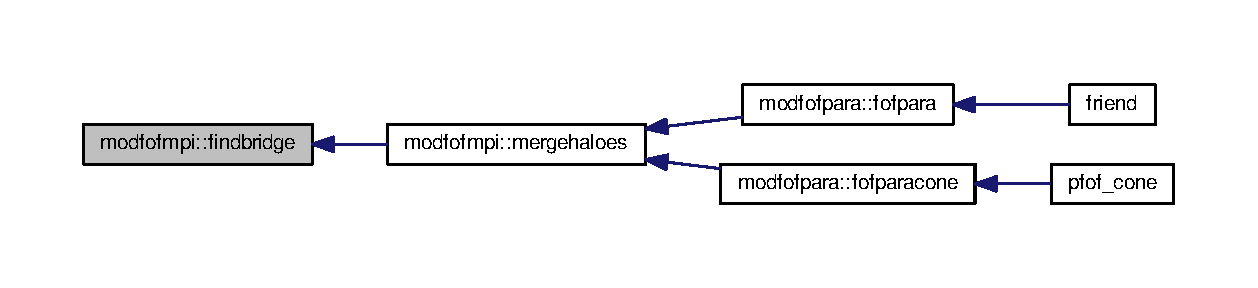
\includegraphics[width=350pt]{classmodfofmpi_ad3a945459cf7b001e4c4e51429eb8f31_icgraph}
\end{center}
\end{figure}


\hypertarget{classmodfofmpi_ac5a219c1a82d90230bcb2b1260adc4b4}{\index{modfofmpi@{modfofmpi}!initmerging@{initmerging}}
\index{initmerging@{initmerging}!modfofmpi@{modfofmpi}}
\subsubsection[{initmerging}]{\setlength{\rightskip}{0pt plus 5cm}subroutine modfofmpi\-::initmerging (
\begin{DoxyParamCaption}
{}
\end{DoxyParamCaption}
)}}\label{classmodfofmpi_ac5a219c1a82d90230bcb2b1260adc4b4}


This routine initializes the merging of halo parts. If the flag value is not 0, the position and halo I\-D of the particle are saved in specific arrays (one array per face). 



Definition at line 100 of file modfofmpi.\-f90.



Here is the caller graph for this function\-:\nopagebreak
\begin{figure}[H]
\begin{center}
\leavevmode
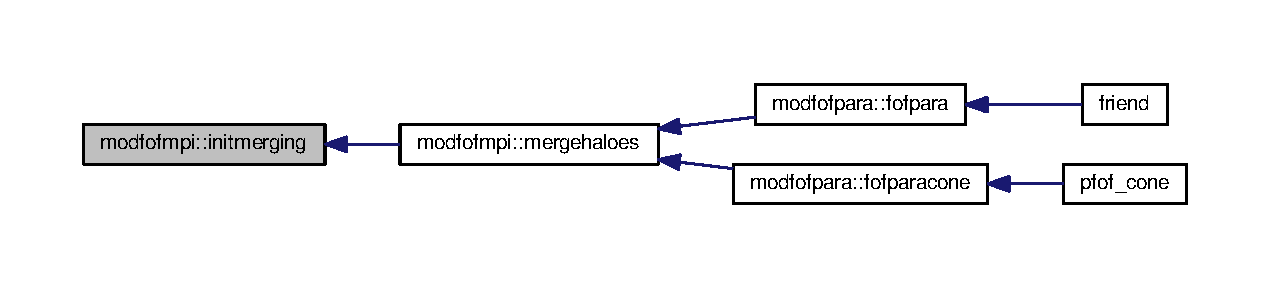
\includegraphics[width=350pt]{classmodfofmpi_ac5a219c1a82d90230bcb2b1260adc4b4_icgraph}
\end{center}
\end{figure}


\hypertarget{classmodfofmpi_a8fbc997f93fd71798027bc6946d3bddb}{\index{modfofmpi@{modfofmpi}!mergehaloes@{mergehaloes}}
\index{mergehaloes@{mergehaloes}!modfofmpi@{modfofmpi}}
\subsubsection[{mergehaloes}]{\setlength{\rightskip}{0pt plus 5cm}subroutine, public modfofmpi\-::mergehaloes (
\begin{DoxyParamCaption}
\item[{real(kind=4), intent(in)}]{perco2, }
\item[{integer, intent(in)}]{mpicomm, }
\item[{logical, intent(in)}]{periodic}
\end{DoxyParamCaption}
)}}\label{classmodfofmpi_a8fbc997f93fd71798027bc6946d3bddb}


This routine merges haloes that extends across several process by setting their halo I\-D to the same value. 


\begin{DoxyParams}[1]{Parameters}
\mbox{\tt in}  & {\em perco2} & Value of the percolation length to the square in normalized units (where the box length in equal to 1.\-0)\\
\hline
\mbox{\tt in}  & {\em mpicomm} & M\-P\-I communicator used in this subroutine\\
\hline
\mbox{\tt in}  & {\em periodic} & .true. for standard p\-Fo\-F and .false. for cone version \\
\hline
\end{DoxyParams}


Definition at line 38 of file modfofmpi.\-f90.



References findbridge(), initmerging(), and setcommonhaloid().



Here is the call graph for this function\-:\nopagebreak
\begin{figure}[H]
\begin{center}
\leavevmode
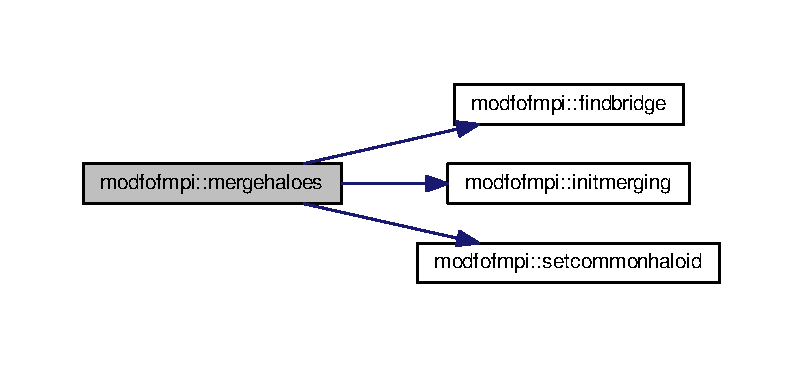
\includegraphics[width=350pt]{classmodfofmpi_a8fbc997f93fd71798027bc6946d3bddb_cgraph}
\end{center}
\end{figure}




Here is the caller graph for this function\-:\nopagebreak
\begin{figure}[H]
\begin{center}
\leavevmode
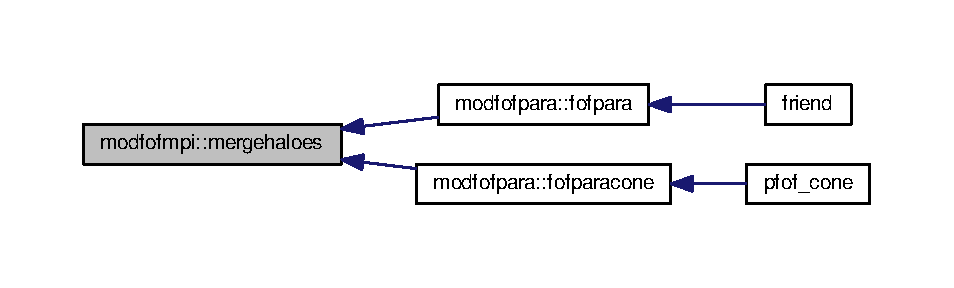
\includegraphics[width=350pt]{classmodfofmpi_a8fbc997f93fd71798027bc6946d3bddb_icgraph}
\end{center}
\end{figure}


\hypertarget{classmodfofmpi_ae5663edf5a2902f952f8d6d3f5c4c8a5}{\index{modfofmpi@{modfofmpi}!setcommonhaloid@{setcommonhaloid}}
\index{setcommonhaloid@{setcommonhaloid}!modfofmpi@{modfofmpi}}
\subsubsection[{setcommonhaloid}]{\setlength{\rightskip}{0pt plus 5cm}subroutine modfofmpi\-::setcommonhaloid (
\begin{DoxyParamCaption}
\item[{integer, intent(in)}]{mpicomm}
\end{DoxyParamCaption}
)}}\label{classmodfofmpi_ae5663edf5a2902f952f8d6d3f5c4c8a5}


Exchanges the halo\-I\-D of the particles located near the faces and edges and set the same halo\-I\-D to each particles that are in the same halo. 


\begin{DoxyParams}[1]{Parameters}
\mbox{\tt in}  & {\em mpicomm} & M\-P\-I communicator used in this subroutine \\
\hline
\end{DoxyParams}


Definition at line 326 of file modfofmpi.\-f90.



Here is the caller graph for this function\-:\nopagebreak
\begin{figure}[H]
\begin{center}
\leavevmode
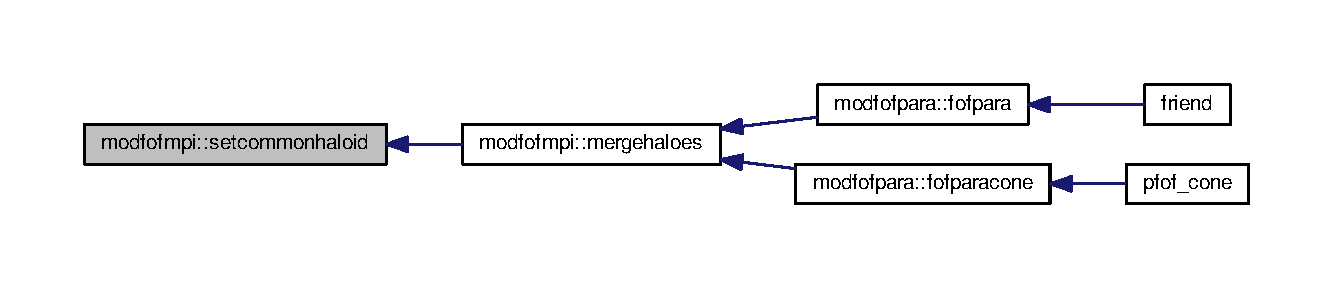
\includegraphics[width=350pt]{classmodfofmpi_ae5663edf5a2902f952f8d6d3f5c4c8a5_icgraph}
\end{center}
\end{figure}




\subsection{Member Data Documentation}
\hypertarget{classmodfofmpi_adb1afd2b26b96173f56ab37495e99e99}{\index{modfofmpi@{modfofmpi}!border@{border}}
\index{border@{border}!modfofmpi@{modfofmpi}}
\subsubsection[{border}]{\setlength{\rightskip}{0pt plus 5cm}integer(kind=1), dimension(\-:), allocatable, public modfofmpi\-::border}}\label{classmodfofmpi_adb1afd2b26b96173f56ab37495e99e99}


Definition at line 24 of file modfofmpi.\-f90.

\hypertarget{classmodfofmpi_a3dffef2edd7b2899179cb3ffffd62430}{\index{modfofmpi@{modfofmpi}!bridgearr@{bridgearr}}
\index{bridgearr@{bridgearr}!modfofmpi@{modfofmpi}}
\subsubsection[{bridgearr}]{\setlength{\rightskip}{0pt plus 5cm}integer(kind=pri), dimension(\-:,\-:), allocatable modfofmpi\-::bridgearr}}\label{classmodfofmpi_a3dffef2edd7b2899179cb3ffffd62430}


Definition at line 20 of file modfofmpi.\-f90.

\hypertarget{classmodfofmpi_a9891331c8f9f2ef3b5532b96129683ac}{\index{modfofmpi@{modfofmpi}!bridgeava@{bridgeava}}
\index{bridgeava@{bridgeava}!modfofmpi@{modfofmpi}}
\subsubsection[{bridgeava}]{\setlength{\rightskip}{0pt plus 5cm}integer(kind=pri), dimension(\-:,\-:), allocatable modfofmpi\-::bridgeava}}\label{classmodfofmpi_a9891331c8f9f2ef3b5532b96129683ac}


Definition at line 20 of file modfofmpi.\-f90.

\hypertarget{classmodfofmpi_a2bdd3864a996f2afb8e49bbcdbd120e5}{\index{modfofmpi@{modfofmpi}!bridgebas@{bridgebas}}
\index{bridgebas@{bridgebas}!modfofmpi@{modfofmpi}}
\subsubsection[{bridgebas}]{\setlength{\rightskip}{0pt plus 5cm}integer(kind=pri), dimension(\-:,\-:), allocatable modfofmpi\-::bridgebas}}\label{classmodfofmpi_a2bdd3864a996f2afb8e49bbcdbd120e5}


Definition at line 21 of file modfofmpi.\-f90.

\hypertarget{classmodfofmpi_a400402d1fc58970ecda00536a07c021c}{\index{modfofmpi@{modfofmpi}!bridgedro@{bridgedro}}
\index{bridgedro@{bridgedro}!modfofmpi@{modfofmpi}}
\subsubsection[{bridgedro}]{\setlength{\rightskip}{0pt plus 5cm}integer(kind=pri), dimension(\-:,\-:), allocatable modfofmpi\-::bridgedro}}\label{classmodfofmpi_a400402d1fc58970ecda00536a07c021c}


Definition at line 21 of file modfofmpi.\-f90.

\hypertarget{classmodfofmpi_a157af8da53311980e23d05748e181a7f}{\index{modfofmpi@{modfofmpi}!bridgegau@{bridgegau}}
\index{bridgegau@{bridgegau}!modfofmpi@{modfofmpi}}
\subsubsection[{bridgegau}]{\setlength{\rightskip}{0pt plus 5cm}integer(kind=pri), dimension(\-:,\-:), allocatable modfofmpi\-::bridgegau}}\label{classmodfofmpi_a157af8da53311980e23d05748e181a7f}


Definition at line 20 of file modfofmpi.\-f90.

\hypertarget{classmodfofmpi_a5a9577c42a1c3c53db8eb603945b530b}{\index{modfofmpi@{modfofmpi}!bridgehau@{bridgehau}}
\index{bridgehau@{bridgehau}!modfofmpi@{modfofmpi}}
\subsubsection[{bridgehau}]{\setlength{\rightskip}{0pt plus 5cm}integer(kind=pri), dimension(\-:,\-:), allocatable modfofmpi\-::bridgehau}}\label{classmodfofmpi_a5a9577c42a1c3c53db8eb603945b530b}


Definition at line 21 of file modfofmpi.\-f90.

\hypertarget{classmodfofmpi_a887d577430624ed6c6e8952b089e0576}{\index{modfofmpi@{modfofmpi}!nbridgearr@{nbridgearr}}
\index{nbridgearr@{nbridgearr}!modfofmpi@{modfofmpi}}
\subsubsection[{nbridgearr}]{\setlength{\rightskip}{0pt plus 5cm}integer(kind=4) modfofmpi\-::nbridgearr}}\label{classmodfofmpi_a887d577430624ed6c6e8952b089e0576}


Definition at line 18 of file modfofmpi.\-f90.

\hypertarget{classmodfofmpi_a2ce30cec8604582ad8aaa26ef19b41cb}{\index{modfofmpi@{modfofmpi}!nbridgeava@{nbridgeava}}
\index{nbridgeava@{nbridgeava}!modfofmpi@{modfofmpi}}
\subsubsection[{nbridgeava}]{\setlength{\rightskip}{0pt plus 5cm}integer(kind=4) modfofmpi\-::nbridgeava}}\label{classmodfofmpi_a2ce30cec8604582ad8aaa26ef19b41cb}


Definition at line 18 of file modfofmpi.\-f90.

\hypertarget{classmodfofmpi_ad71e96722537b8de69afdb8f68028e8b}{\index{modfofmpi@{modfofmpi}!nbridgebas@{nbridgebas}}
\index{nbridgebas@{nbridgebas}!modfofmpi@{modfofmpi}}
\subsubsection[{nbridgebas}]{\setlength{\rightskip}{0pt plus 5cm}integer(kind=4) modfofmpi\-::nbridgebas}}\label{classmodfofmpi_ad71e96722537b8de69afdb8f68028e8b}


Definition at line 19 of file modfofmpi.\-f90.

\hypertarget{classmodfofmpi_a0253e42a34623e4816f27522252d1e29}{\index{modfofmpi@{modfofmpi}!nbridgedro@{nbridgedro}}
\index{nbridgedro@{nbridgedro}!modfofmpi@{modfofmpi}}
\subsubsection[{nbridgedro}]{\setlength{\rightskip}{0pt plus 5cm}integer(kind=4) modfofmpi\-::nbridgedro}}\label{classmodfofmpi_a0253e42a34623e4816f27522252d1e29}


Definition at line 19 of file modfofmpi.\-f90.

\hypertarget{classmodfofmpi_a000b4f4f0140c24648780b86d56698cf}{\index{modfofmpi@{modfofmpi}!nbridgegau@{nbridgegau}}
\index{nbridgegau@{nbridgegau}!modfofmpi@{modfofmpi}}
\subsubsection[{nbridgegau}]{\setlength{\rightskip}{0pt plus 5cm}integer(kind=4) modfofmpi\-::nbridgegau}}\label{classmodfofmpi_a000b4f4f0140c24648780b86d56698cf}


Definition at line 18 of file modfofmpi.\-f90.

\hypertarget{classmodfofmpi_a81ecc186519e9addf2dbf7ec92e32d23}{\index{modfofmpi@{modfofmpi}!nbridgehau@{nbridgehau}}
\index{nbridgehau@{nbridgehau}!modfofmpi@{modfofmpi}}
\subsubsection[{nbridgehau}]{\setlength{\rightskip}{0pt plus 5cm}integer(kind=4) modfofmpi\-::nbridgehau}}\label{classmodfofmpi_a81ecc186519e9addf2dbf7ec92e32d23}


Definition at line 19 of file modfofmpi.\-f90.

\hypertarget{classmodfofmpi_a9b2252c09a83a3f47fc6aec6462a68dc}{\index{modfofmpi@{modfofmpi}!nflagloc@{nflagloc}}
\index{nflagloc@{nflagloc}!modfofmpi@{modfofmpi}}
\subsubsection[{nflagloc}]{\setlength{\rightskip}{0pt plus 5cm}integer(kind=4), dimension(6), public modfofmpi\-::nflagloc}}\label{classmodfofmpi_a9b2252c09a83a3f47fc6aec6462a68dc}


Definition at line 23 of file modfofmpi.\-f90.

\hypertarget{classmodfofmpi_aa8c0fc08baf8d208d7e2cddd0600ff99}{\index{modfofmpi@{modfofmpi}!nflagrecv@{nflagrecv}}
\index{nflagrecv@{nflagrecv}!modfofmpi@{modfofmpi}}
\subsubsection[{nflagrecv}]{\setlength{\rightskip}{0pt plus 5cm}integer(kind=4), dimension(6) modfofmpi\-::nflagrecv}}\label{classmodfofmpi_aa8c0fc08baf8d208d7e2cddd0600ff99}


Definition at line 22 of file modfofmpi.\-f90.

\hypertarget{classmodfofmpi_a240c326e64798f0d4f7fd2a785eaddfb}{\index{modfofmpi@{modfofmpi}!posarr@{posarr}}
\index{posarr@{posarr}!modfofmpi@{modfofmpi}}
\subsubsection[{posarr}]{\setlength{\rightskip}{0pt plus 5cm}real (kind=4), dimension(\-:,\-:), allocatable modfofmpi\-::posarr}}\label{classmodfofmpi_a240c326e64798f0d4f7fd2a785eaddfb}


Definition at line 16 of file modfofmpi.\-f90.

\hypertarget{classmodfofmpi_a91f992ee7447a7fb3c5430233f3f39ab}{\index{modfofmpi@{modfofmpi}!posava@{posava}}
\index{posava@{posava}!modfofmpi@{modfofmpi}}
\subsubsection[{posava}]{\setlength{\rightskip}{0pt plus 5cm}real (kind=4), dimension(\-:,\-:), allocatable modfofmpi\-::posava}}\label{classmodfofmpi_a91f992ee7447a7fb3c5430233f3f39ab}


Definition at line 16 of file modfofmpi.\-f90.

\hypertarget{classmodfofmpi_abd8afe0852ff1d0298955d285cb4f001}{\index{modfofmpi@{modfofmpi}!posbas@{posbas}}
\index{posbas@{posbas}!modfofmpi@{modfofmpi}}
\subsubsection[{posbas}]{\setlength{\rightskip}{0pt plus 5cm}real (kind=4), dimension(\-:,\-:), allocatable modfofmpi\-::posbas}}\label{classmodfofmpi_abd8afe0852ff1d0298955d285cb4f001}


Definition at line 16 of file modfofmpi.\-f90.

\hypertarget{classmodfofmpi_a1ca3754d2490a28a6596589818c19aba}{\index{modfofmpi@{modfofmpi}!posdro@{posdro}}
\index{posdro@{posdro}!modfofmpi@{modfofmpi}}
\subsubsection[{posdro}]{\setlength{\rightskip}{0pt plus 5cm}real (kind=4), dimension(\-:,\-:), allocatable modfofmpi\-::posdro}}\label{classmodfofmpi_a1ca3754d2490a28a6596589818c19aba}


Definition at line 16 of file modfofmpi.\-f90.

\hypertarget{classmodfofmpi_a420a314f84492aec68a773c09730981d}{\index{modfofmpi@{modfofmpi}!posgau@{posgau}}
\index{posgau@{posgau}!modfofmpi@{modfofmpi}}
\subsubsection[{posgau}]{\setlength{\rightskip}{0pt plus 5cm}real (kind=4), dimension(\-:,\-:), allocatable modfofmpi\-::posgau}}\label{classmodfofmpi_a420a314f84492aec68a773c09730981d}


Definition at line 16 of file modfofmpi.\-f90.

\hypertarget{classmodfofmpi_a940b15087397a154e933785ff862d1aa}{\index{modfofmpi@{modfofmpi}!poshau@{poshau}}
\index{poshau@{poshau}!modfofmpi@{modfofmpi}}
\subsubsection[{poshau}]{\setlength{\rightskip}{0pt plus 5cm}real (kind=4), dimension(\-:,\-:), allocatable modfofmpi\-::poshau}}\label{classmodfofmpi_a940b15087397a154e933785ff862d1aa}


Definition at line 16 of file modfofmpi.\-f90.

\hypertarget{classmodfofmpi_adc11b8c24e402c222ddf9d339aece63c}{\index{modfofmpi@{modfofmpi}!strarr@{strarr}}
\index{strarr@{strarr}!modfofmpi@{modfofmpi}}
\subsubsection[{strarr}]{\setlength{\rightskip}{0pt plus 5cm}integer(kind=pri), dimension(\-:), allocatable modfofmpi\-::strarr}}\label{classmodfofmpi_adc11b8c24e402c222ddf9d339aece63c}


Definition at line 17 of file modfofmpi.\-f90.

\hypertarget{classmodfofmpi_a2cc07767e1b2a2462fc2eeaaef5f5b0a}{\index{modfofmpi@{modfofmpi}!strava@{strava}}
\index{strava@{strava}!modfofmpi@{modfofmpi}}
\subsubsection[{strava}]{\setlength{\rightskip}{0pt plus 5cm}integer(kind=pri), dimension(\-:), allocatable modfofmpi\-::strava}}\label{classmodfofmpi_a2cc07767e1b2a2462fc2eeaaef5f5b0a}


Definition at line 17 of file modfofmpi.\-f90.

\hypertarget{classmodfofmpi_a18f63a61d3cf10a560030f18385646d6}{\index{modfofmpi@{modfofmpi}!strbas@{strbas}}
\index{strbas@{strbas}!modfofmpi@{modfofmpi}}
\subsubsection[{strbas}]{\setlength{\rightskip}{0pt plus 5cm}integer(kind=pri), dimension(\-:), allocatable modfofmpi\-::strbas}}\label{classmodfofmpi_a18f63a61d3cf10a560030f18385646d6}


Definition at line 17 of file modfofmpi.\-f90.

\hypertarget{classmodfofmpi_a6f52fb3f19368ce1dbad562162f6d4b5}{\index{modfofmpi@{modfofmpi}!strdro@{strdro}}
\index{strdro@{strdro}!modfofmpi@{modfofmpi}}
\subsubsection[{strdro}]{\setlength{\rightskip}{0pt plus 5cm}integer(kind=pri), dimension(\-:), allocatable modfofmpi\-::strdro}}\label{classmodfofmpi_a6f52fb3f19368ce1dbad562162f6d4b5}


Definition at line 17 of file modfofmpi.\-f90.

\hypertarget{classmodfofmpi_a59d3a040e03ea0312701cf16ded04071}{\index{modfofmpi@{modfofmpi}!strgau@{strgau}}
\index{strgau@{strgau}!modfofmpi@{modfofmpi}}
\subsubsection[{strgau}]{\setlength{\rightskip}{0pt plus 5cm}integer(kind=pri), dimension(\-:), allocatable modfofmpi\-::strgau}}\label{classmodfofmpi_a59d3a040e03ea0312701cf16ded04071}


Definition at line 17 of file modfofmpi.\-f90.

\hypertarget{classmodfofmpi_a9ace6e4f0b23785f3b93fe1812b07c08}{\index{modfofmpi@{modfofmpi}!strhau@{strhau}}
\index{strhau@{strhau}!modfofmpi@{modfofmpi}}
\subsubsection[{strhau}]{\setlength{\rightskip}{0pt plus 5cm}integer(kind=pri), dimension(\-:), allocatable modfofmpi\-::strhau}}\label{classmodfofmpi_a9ace6e4f0b23785f3b93fe1812b07c08}


Definition at line 17 of file modfofmpi.\-f90.

\hypertarget{classmodfofmpi_ada00af1a25f50e826521e9b2a7ecb633}{\index{modfofmpi@{modfofmpi}!strrec@{strrec}}
\index{strrec@{strrec}!modfofmpi@{modfofmpi}}
\subsubsection[{strrec}]{\setlength{\rightskip}{0pt plus 5cm}integer(kind=pri), dimension(\-:), allocatable modfofmpi\-::strrec}}\label{classmodfofmpi_ada00af1a25f50e826521e9b2a7ecb633}


Definition at line 17 of file modfofmpi.\-f90.



The documentation for this module was generated from the following file\-:\begin{DoxyCompactItemize}
\item 
/home/roy/\-Travail/\-Devel/\-Cosmologie/\-Pfof/branches/\-Modif\-Struct/common/src/\hyperlink{modfofmpi_8f90}{modfofmpi.\-f90}\end{DoxyCompactItemize}

\hypertarget{classmodfofpara}{\section{modfofpara Module Reference}
\label{classmodfofpara}\index{modfofpara@{modfofpara}}
}


This module contains the serial F\-O\-F algorithm.  


\subsection*{Public Member Functions}
\begin{DoxyCompactItemize}
\item 
subroutine, public \hyperlink{classmodfofpara_a4ec0353cad472761978bbabf6846ac4f}{fofpara} ()
\begin{DoxyCompactList}\small\item\em Parallel F\-O\-F subroutine Finds haloes on each process then apply the merging process for haloes that extend across several processes. \end{DoxyCompactList}\item 
subroutine \hyperlink{classmodfofpara_a5294ecab752fb3cfbea3bec7cd28a29a}{init} (n, np, ngpp, x, pile, adfirst, npcase, xmin, ymin, zmin, t)
\begin{DoxyCompactList}\small\item\em Initialize the stacks of pointers for local friends of friends.\par
 The whole domain is divided into t$^\wedge$3 cubes, where t is the resolution of the simulation analized times the refine\-\_\-fof factor.\par
 Each process will implicitly considere only its subdomains because every particles treated by the process is located in the same subdomain.\par
 This routine initializes one stack of \char`\"{}pointers\char`\"{} to the index of the particles located in each cube. \end{DoxyCompactList}\item 
subroutine \hyperlink{classmodfofpara_a033a2820dd29f107782b566ca298bde4}{fofparacone} ()
\begin{DoxyCompactList}\small\item\em Parallel F\-O\-F subroutine Finds haloes on each process then apply the merging process for haloes that extend across several processes. \end{DoxyCompactList}\item 
subroutine \hyperlink{classmodfofpara_afdd2abc340cad047a13ebbb62f1bafdc}{init} (n, np, ngpp, x, pile, adfirst, npcase, xmin, ymin, zmin, t, edgem1)
\begin{DoxyCompactList}\small\item\em Initialize the stacks of pointers for local friends of friends.\par
 The whole domain is divided into t$^\wedge$3 cubes, where t is the resolution of the simulation analized times the refine\-\_\-fof factor.\par
 Each process will implicitly considere only its subdomains because every particles treated by the process is located in the same subdomain.\par
 This routine initializes one stack of \char`\"{}pointers\char`\"{} to the index of the particles located in each cube. \end{DoxyCompactList}\item 
subroutine \hyperlink{classmodfofpara_aae8bee067b5066b64d8799e78efa239c}{computeminmax} ()
\end{DoxyCompactItemize}


\subsection{Detailed Description}
This module contains the serial F\-O\-F algorithm. 

Authors\-: E. Audit, F. Roy, V. Bouillot 

Definition at line 8 of file modfofpara.\-f90.



\subsection{Member Function/\-Subroutine Documentation}
\hypertarget{classmodfofpara_aae8bee067b5066b64d8799e78efa239c}{\index{modfofpara@{modfofpara}!computeminmax@{computeminmax}}
\index{computeminmax@{computeminmax}!modfofpara@{modfofpara}}
\subsubsection[{computeminmax}]{\setlength{\rightskip}{0pt plus 5cm}subroutine modfofpara\-::computeminmax (
\begin{DoxyParamCaption}
{}
\end{DoxyParamCaption}
)}}\label{classmodfofpara_aae8bee067b5066b64d8799e78efa239c}


Definition at line 590 of file modfofpara.\-f90.



Here is the caller graph for this function\-:\nopagebreak
\begin{figure}[H]
\begin{center}
\leavevmode
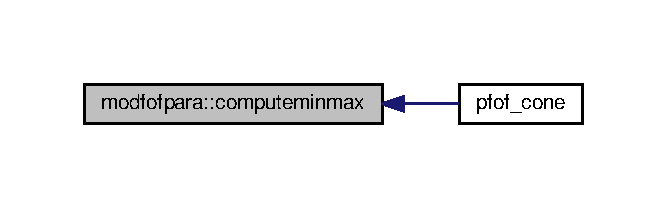
\includegraphics[width=320pt]{classmodfofpara_aae8bee067b5066b64d8799e78efa239c_icgraph}
\end{center}
\end{figure}


\hypertarget{classmodfofpara_a4ec0353cad472761978bbabf6846ac4f}{\index{modfofpara@{modfofpara}!fofpara@{fofpara}}
\index{fofpara@{fofpara}!modfofpara@{modfofpara}}
\subsubsection[{fofpara}]{\setlength{\rightskip}{0pt plus 5cm}subroutine, public modfofpara\-::fofpara (
\begin{DoxyParamCaption}
{}
\end{DoxyParamCaption}
)}}\label{classmodfofpara_a4ec0353cad472761978bbabf6846ac4f}


Parallel F\-O\-F subroutine Finds haloes on each process then apply the merging process for haloes that extend across several processes. 



Definition at line 23 of file modfofpara.\-f90.



References modhalo\-::computecom(), modhalo\-::computeradius(), modhalo\-::gatherhaloes(), modwritehalo\-::h5writehalopart(), init(), modfofmpi\-::mergehaloes(), modwritehalo\-::mpih5writehalomass(), and modhalo\-::selecthaloes().



Here is the call graph for this function\-:\nopagebreak
\begin{figure}[H]
\begin{center}
\leavevmode
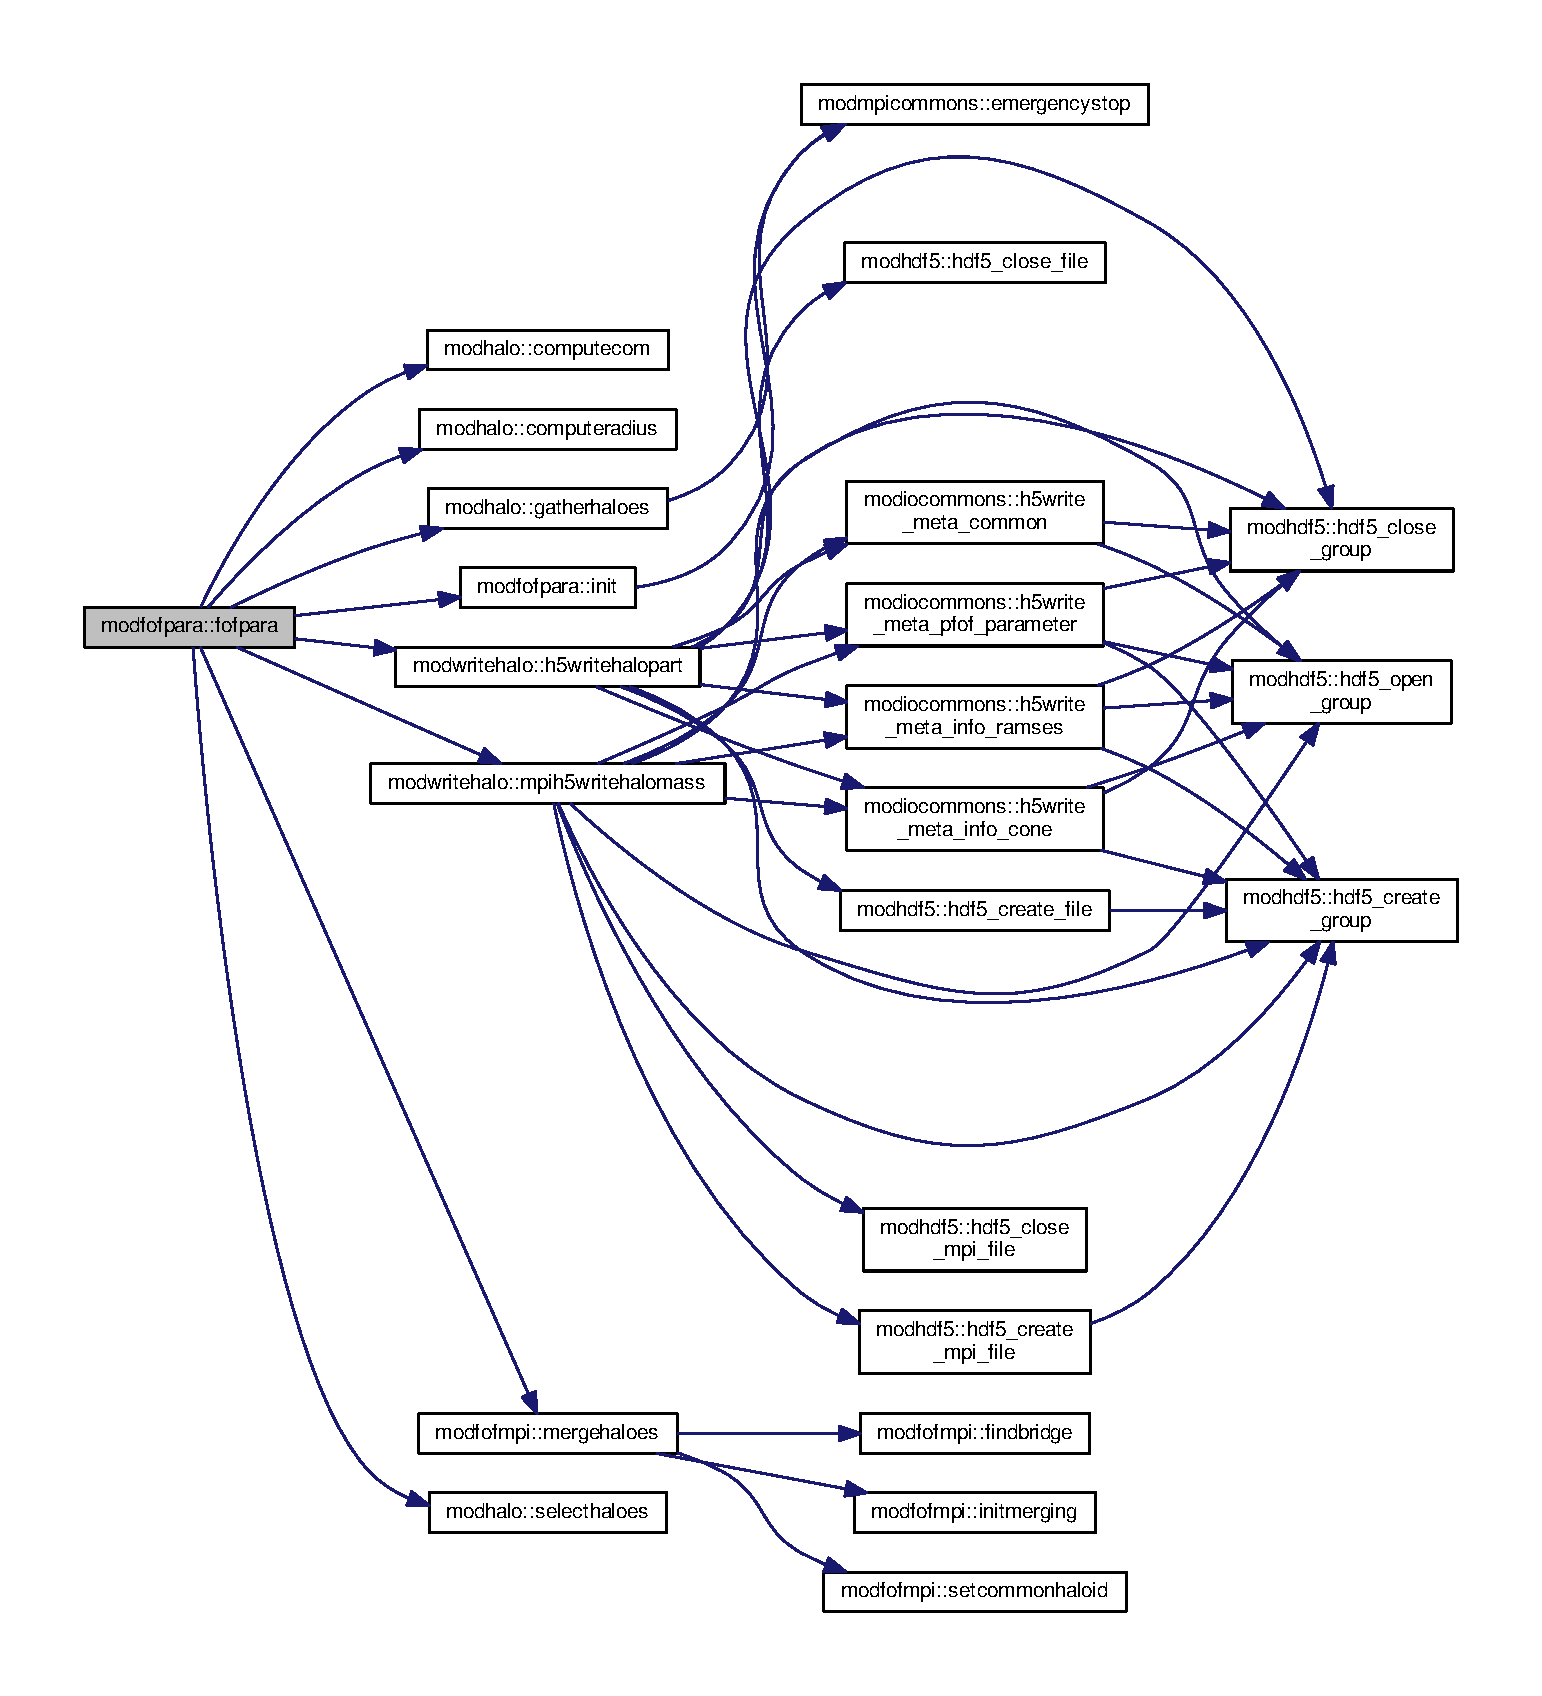
\includegraphics[width=350pt]{classmodfofpara_a4ec0353cad472761978bbabf6846ac4f_cgraph}
\end{center}
\end{figure}




Here is the caller graph for this function\-:\nopagebreak
\begin{figure}[H]
\begin{center}
\leavevmode
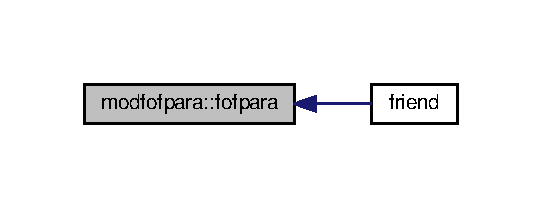
\includegraphics[width=260pt]{classmodfofpara_a4ec0353cad472761978bbabf6846ac4f_icgraph}
\end{center}
\end{figure}


\hypertarget{classmodfofpara_a033a2820dd29f107782b566ca298bde4}{\index{modfofpara@{modfofpara}!fofparacone@{fofparacone}}
\index{fofparacone@{fofparacone}!modfofpara@{modfofpara}}
\subsubsection[{fofparacone}]{\setlength{\rightskip}{0pt plus 5cm}subroutine modfofpara\-::fofparacone (
\begin{DoxyParamCaption}
{}
\end{DoxyParamCaption}
)}}\label{classmodfofpara_a033a2820dd29f107782b566ca298bde4}


Parallel F\-O\-F subroutine Finds haloes on each process then apply the merging process for haloes that extend across several processes. 



Definition at line 19 of file modfofpara.\-f90.



References modhalo\-::computecom(), modhalo\-::computeradius(), modhalo\-::gatherhaloes(), modwritehalo\-::h5writehalopart(), init(), modfofmpi\-::mergehaloes(), modwritehalo\-::mpih5writehalomass(), and modhalo\-::selecthaloes().



Here is the call graph for this function\-:\nopagebreak
\begin{figure}[H]
\begin{center}
\leavevmode
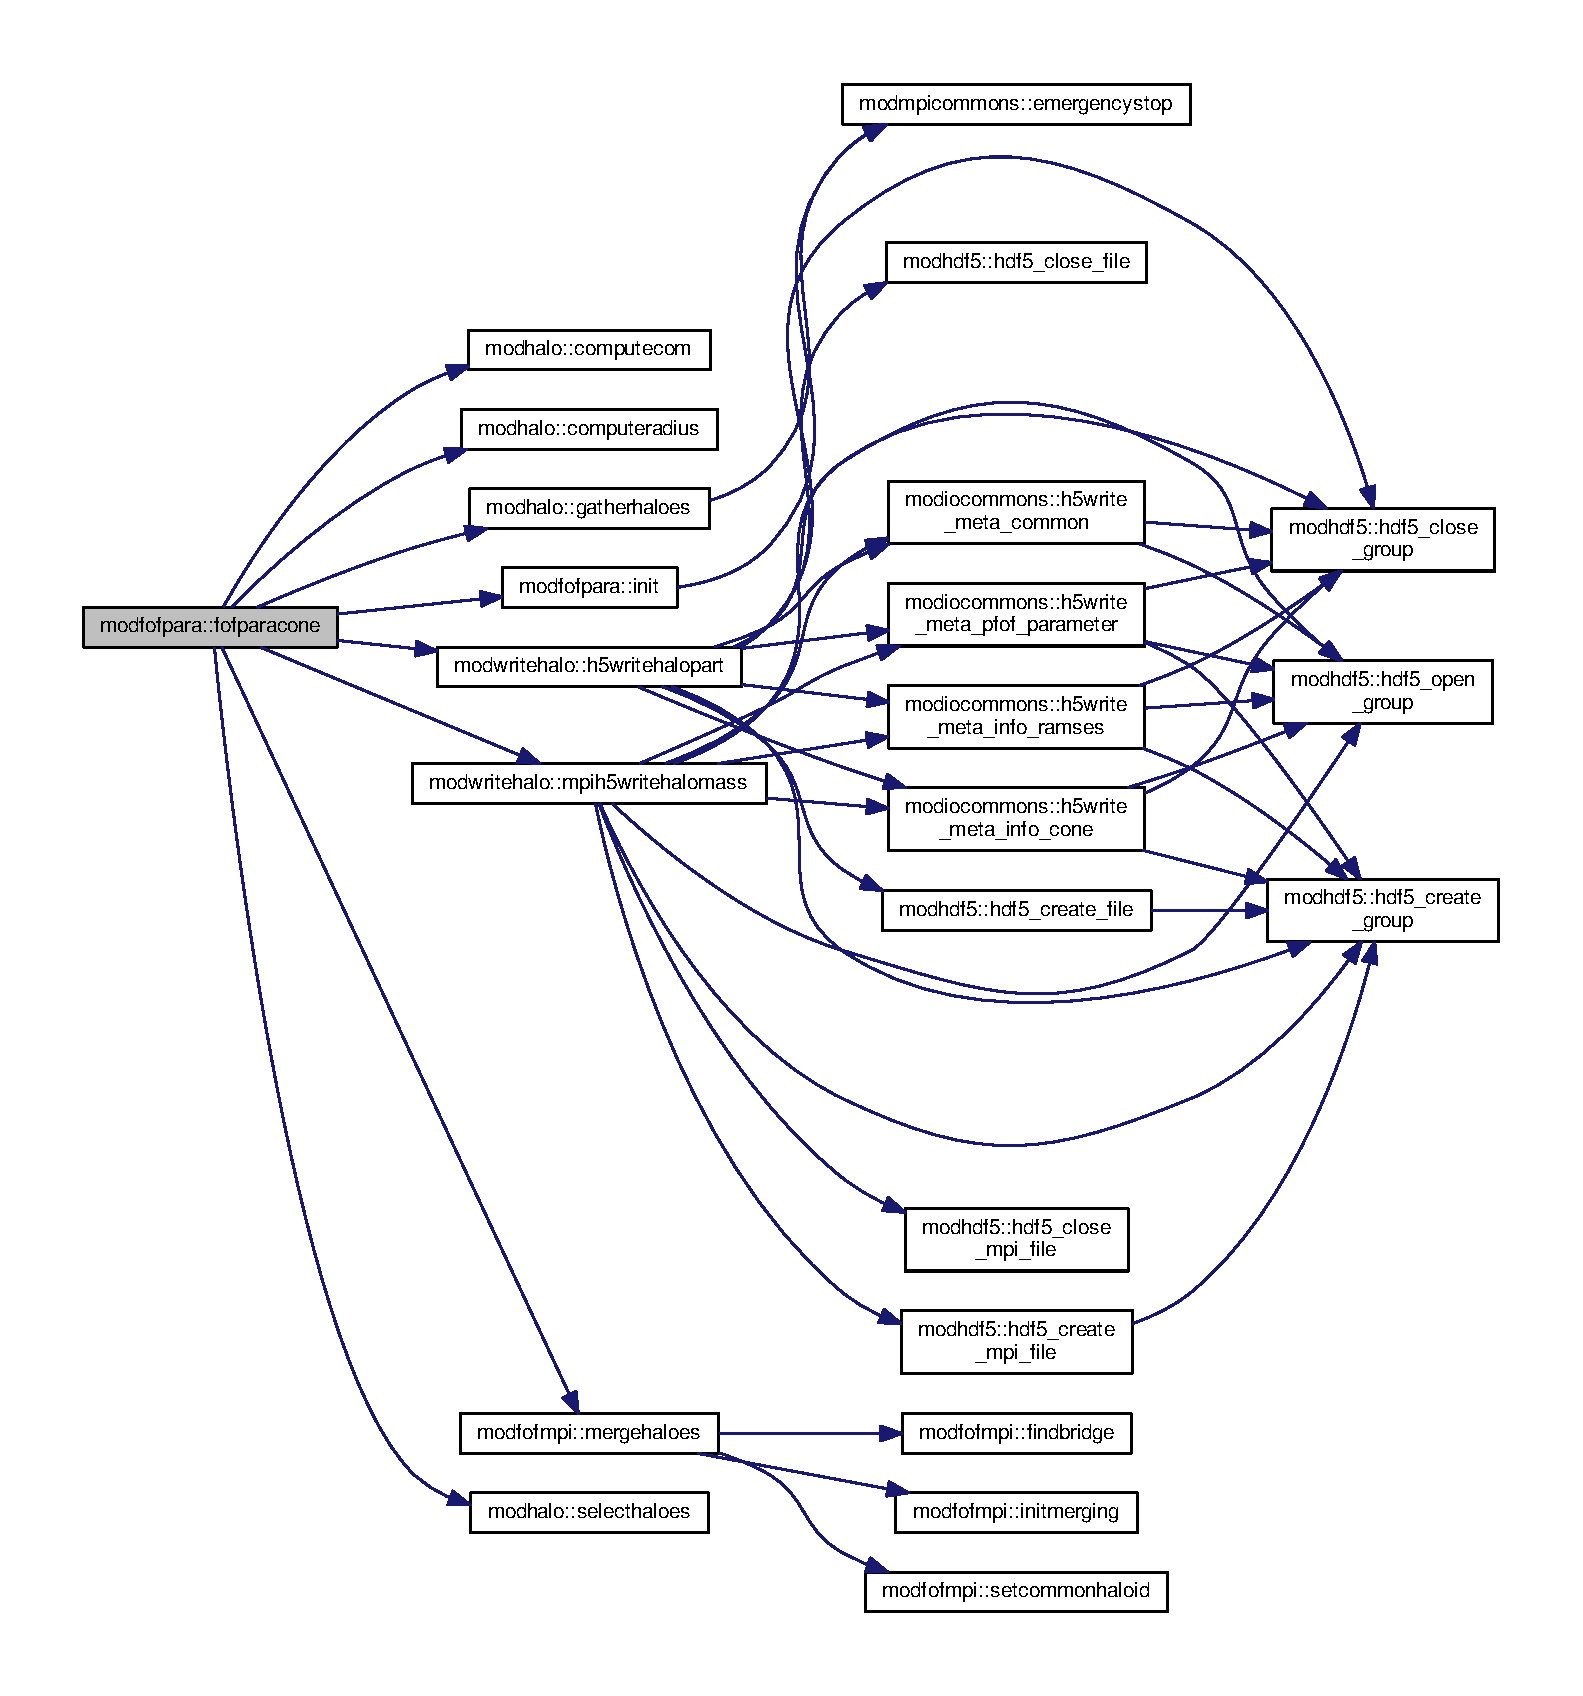
\includegraphics[width=350pt]{classmodfofpara_a033a2820dd29f107782b566ca298bde4_cgraph}
\end{center}
\end{figure}




Here is the caller graph for this function\-:\nopagebreak
\begin{figure}[H]
\begin{center}
\leavevmode
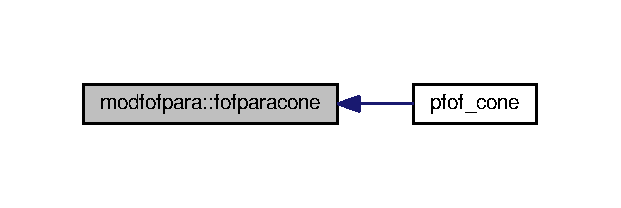
\includegraphics[width=298pt]{classmodfofpara_a033a2820dd29f107782b566ca298bde4_icgraph}
\end{center}
\end{figure}


\hypertarget{classmodfofpara_afdd2abc340cad047a13ebbb62f1bafdc}{\index{modfofpara@{modfofpara}!init@{init}}
\index{init@{init}!modfofpara@{modfofpara}}
\subsubsection[{init}]{\setlength{\rightskip}{0pt plus 5cm}subroutine modfofpara\-::init (
\begin{DoxyParamCaption}
\item[{integer(kind=4), intent(in)}]{n, }
\item[{integer(kind=4), intent(in)}]{np, }
\item[{integer(kind=4), intent(in)}]{ngpp, }
\item[{real(kind=4), dimension(3,np), intent(in)}]{x, }
\item[{integer(kind=4), dimension(np), intent(out)}]{pile, }
\item[{integer(kind=4), dimension(ngpp), intent(out)}]{adfirst, }
\item[{integer(kind=4), dimension(ngpp), intent(out)}]{npcase, }
\item[{real(kind=4)}]{xmin, }
\item[{real(kind=4)}]{ymin, }
\item[{real(kind=4)}]{zmin, }
\item[{real(kind=4), intent(in)}]{t, }
\item[{real(kind=4), intent(in)}]{edgem1}
\end{DoxyParamCaption}
)}}\label{classmodfofpara_afdd2abc340cad047a13ebbb62f1bafdc}


Initialize the stacks of pointers for local friends of friends.\par
 The whole domain is divided into t$^\wedge$3 cubes, where t is the resolution of the simulation analized times the refine\-\_\-fof factor.\par
 Each process will implicitly considere only its subdomains because every particles treated by the process is located in the same subdomain.\par
 This routine initializes one stack of \char`\"{}pointers\char`\"{} to the index of the particles located in each cube. 


\begin{DoxyParams}[1]{Parameters}
\mbox{\tt in}  & {\em n} & number of \char`\"{}cube\char`\"{} in each dimension in a subdomain, i.\-e. there are n$^\wedge$3 cubes in a subdomain\\
\hline
\mbox{\tt in}  & {\em np} & number of particles in the subdomain\\
\hline
\mbox{\tt in}  & {\em ngpp} & number of \char`\"{}\-F\-O\-F\char`\"{} cubes in the subdomain\\
\hline
\mbox{\tt in}  & {\em x} & positions of the particles\\
\hline
\mbox{\tt in}  & {\em t} & resolution of the cosmological simulation times refine\-\_\-fof factor\\
\hline
\mbox{\tt out}  & {\em npcase} & number of particles in each cube\\
\hline
\mbox{\tt out}  & {\em adfirst} & index of the first particle to examine in the cube\\
\hline
\mbox{\tt out}  & {\em pile} & stack of indices \\
\hline
\end{DoxyParams}


Definition at line 507 of file modfofpara.\-f90.



References modmpicommons\-::emergencystop().



Here is the call graph for this function\-:\nopagebreak
\begin{figure}[H]
\begin{center}
\leavevmode
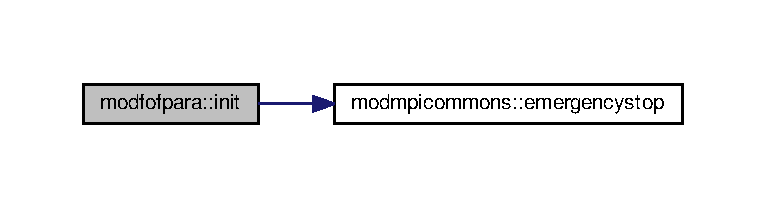
\includegraphics[width=350pt]{classmodfofpara_afdd2abc340cad047a13ebbb62f1bafdc_cgraph}
\end{center}
\end{figure}


\hypertarget{classmodfofpara_a5294ecab752fb3cfbea3bec7cd28a29a}{\index{modfofpara@{modfofpara}!init@{init}}
\index{init@{init}!modfofpara@{modfofpara}}
\subsubsection[{init}]{\setlength{\rightskip}{0pt plus 5cm}subroutine modfofpara\-::init (
\begin{DoxyParamCaption}
\item[{integer(kind=4), intent(in)}]{n, }
\item[{integer(kind=4), intent(in)}]{np, }
\item[{integer(kind=4), intent(in)}]{ngpp, }
\item[{real(kind=4), dimension(3,np), intent(in)}]{x, }
\item[{integer(kind=4), dimension(np), intent(out)}]{pile, }
\item[{integer(kind=4), dimension(ngpp), intent(out)}]{adfirst, }
\item[{integer(kind=4), dimension(ngpp), intent(out)}]{npcase, }
\item[{real(kind=4), intent(in)}]{xmin, }
\item[{real(kind=4), intent(in)}]{ymin, }
\item[{real(kind=4), intent(in)}]{zmin, }
\item[{real(kind=4), intent(in)}]{t}
\end{DoxyParamCaption}
)}}\label{classmodfofpara_a5294ecab752fb3cfbea3bec7cd28a29a}


Initialize the stacks of pointers for local friends of friends.\par
 The whole domain is divided into t$^\wedge$3 cubes, where t is the resolution of the simulation analized times the refine\-\_\-fof factor.\par
 Each process will implicitly considere only its subdomains because every particles treated by the process is located in the same subdomain.\par
 This routine initializes one stack of \char`\"{}pointers\char`\"{} to the index of the particles located in each cube. 


\begin{DoxyParams}[1]{Parameters}
\mbox{\tt in}  & {\em n} & number of \char`\"{}cube\char`\"{} in each dimension in a subdomain, i.\-e. there are n$^\wedge$3 cubes in a subdomain\\
\hline
\mbox{\tt in}  & {\em np} & number of particles in the subdomain\\
\hline
\mbox{\tt in}  & {\em ngpp} & number of \char`\"{}\-F\-O\-F\char`\"{} cubes in the subdomain\\
\hline
\mbox{\tt in}  & {\em x} & positions of the particles\\
\hline
\mbox{\tt in}  & {\em zmin} & minimum x,y and z of the subdomain\\
\hline
\mbox{\tt in}  & {\em t} & resolution of the cosmological simulation times refine\-\_\-fof factor\\
\hline
\mbox{\tt out}  & {\em npcase} & number of particles in each cube\\
\hline
\mbox{\tt out}  & {\em adfirst} & index of the first particle to examine in the cube\\
\hline
\mbox{\tt out}  & {\em pile} & stack of indices \\
\hline
\end{DoxyParams}


Definition at line 458 of file modfofpara.\-f90.



References modmpicommons\-::emergencystop().



Here is the call graph for this function\-:\nopagebreak
\begin{figure}[H]
\begin{center}
\leavevmode
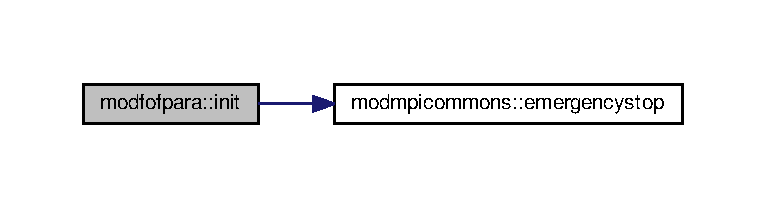
\includegraphics[width=350pt]{classmodfofpara_a5294ecab752fb3cfbea3bec7cd28a29a_cgraph}
\end{center}
\end{figure}




Here is the caller graph for this function\-:\nopagebreak
\begin{figure}[H]
\begin{center}
\leavevmode
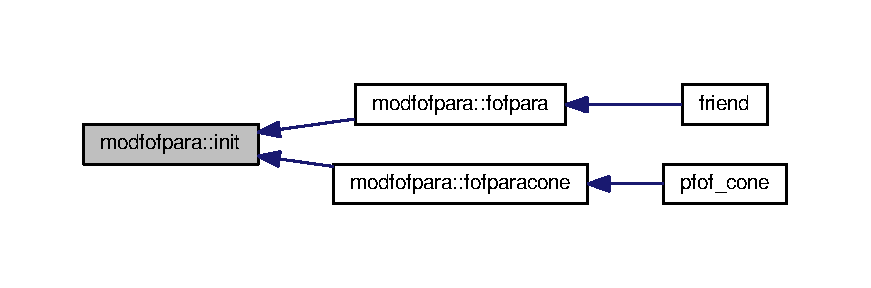
\includegraphics[width=350pt]{classmodfofpara_a5294ecab752fb3cfbea3bec7cd28a29a_icgraph}
\end{center}
\end{figure}




The documentation for this module was generated from the following file\-:\begin{DoxyCompactItemize}
\item 
/home/roy/\-Travail/\-Devel/\-Cosmologie/\-Pfof/branches/\-Modif\-Struct/pfof\-\_\-snap/src/\hyperlink{pfof__snap_2src_2modfofpara_8f90}{modfofpara.\-f90}\end{DoxyCompactItemize}

\hypertarget{classmodhalo}{\section{modhalo Module Reference}
\label{classmodhalo}\index{modhalo@{modhalo}}
}


This module contains subroutines used to gather haloes on the differents processes and compute some observables.  


\subsection*{Public Member Functions}
\begin{DoxyCompactItemize}
\item 
subroutine, public \hyperlink{classmodhalo_a1ffd35b4853d5d5c196678d253d43ae3}{gatherhaloes} (mpicomm, param)
\begin{DoxyCompactList}\small\item\em Exchange the particles so that particles belonging to one halo are gathered on the same process. \end{DoxyCompactList}\item 
subroutine, public \hyperlink{classmodhalo_ac468bdd056bc7c1db7e5338bce89ed5b}{selecthaloes} (param)
\item 
subroutine, public \hyperlink{classmodhalo_a2f8c1fd1c7fd4704ef7b80cbd4f6272a}{computecom} (periodic)
\item 
subroutine, public \hyperlink{classmodhalo_a891d00fd31e67d5669ac52117cf13034}{computeradius} (periodic)
\end{DoxyCompactItemize}
\subsection*{Public Attributes}
\begin{DoxyCompactItemize}
\item 
integer(kind=4), public \hyperlink{classmodhalo_aa38fb84fd13087a625a48555740b9f2d}{halonb}
\begin{DoxyCompactList}\small\item\em local number of haloes \end{DoxyCompactList}\item 
integer(kind=4), public \hyperlink{classmodhalo_ad416ab5cda1e3a837e8392415f305ffd}{halonb\-\_\-all}
\begin{DoxyCompactList}\small\item\em global number of haloes \end{DoxyCompactList}\item 
integer(kind=4), public \hyperlink{classmodhalo_aa2c5c12e5bd7198d5571d7ff832ffa38}{halopartnb}
\begin{DoxyCompactList}\small\item\em number of particles belonging to one of the local haloes \end{DoxyCompactList}\item 
integer(kind=4), public \hyperlink{classmodhalo_aea1cd3a6f28ec75795cb930326cc2744}{final\-\_\-local\-\_\-npart}
\begin{DoxyCompactList}\small\item\em number of particles after the particles have been exchanged to gather them by haloes \end{DoxyCompactList}\item 
integer(kind=4), dimension(\-:), \\*
allocatable, public \hyperlink{classmodhalo_ad235215a443e0871d790576ff1ad77c2}{halomass}
\begin{DoxyCompactList}\small\item\em mass of the haloes \end{DoxyCompactList}\item 
integer(kind=pri), dimension(\-:), \\*
allocatable, public \hyperlink{classmodhalo_a123a9c168d495f9bbe3d1e25be025105}{haloid}
\begin{DoxyCompactList}\small\item\em I\-D of the haloes. \end{DoxyCompactList}\item 
integer(kind=pri), dimension(\-:), \\*
allocatable, public \hyperlink{classmodhalo_a2355dfa04d7ba9d48277d3f4d1e44a64}{halopartid}
\begin{DoxyCompactList}\small\item\em I\-D of the particles belonging to a halo. \end{DoxyCompactList}\item 
integer(kind=pri), dimension(\-:), \\*
allocatable, public \hyperlink{classmodhalo_a3c78e77057ed6c209d4081c8d559aed3}{halopartramsesid}
\begin{DoxyCompactList}\small\item\em R\-A\-M\-S\-E\-S I\-D of the particles belonging to a halo, used only for lightcone halo. \end{DoxyCompactList}\item 
integer(kind=4), dimension(\-:), \\*
allocatable, public \hyperlink{classmodhalo_a5dfc215badbd6aa90e9330266a673923}{halosubhalonb}
\begin{DoxyCompactList}\small\item\em number of subhalo for each halo \end{DoxyCompactList}\item 
real(kind=4), dimension(\-:,\-:), \\*
allocatable, public \hyperlink{classmodhalo_a92a746382aef848ff806f8eead8ca9e5}{halopartpos}
\begin{DoxyCompactList}\small\item\em position of the particles belonging to one of the local haloes \end{DoxyCompactList}\item 
real(kind=4), dimension(\-:,\-:), \\*
allocatable, public \hyperlink{classmodhalo_abd1eee90e1638db519b34633410ff9d1}{halopartvel}
\begin{DoxyCompactList}\small\item\em velocity of the particles belonging to one of the local haloes \end{DoxyCompactList}\item 
real(kind=4), dimension(\-:), \\*
allocatable, public \hyperlink{classmodhalo_a5d7a2e398703c4b5e5826d4e80638f6b}{halopartpot}
\begin{DoxyCompactList}\small\item\em potential of the particles belonging to one of the local haloes \end{DoxyCompactList}\item 
real(kind=4), dimension(\-:,\-:), \\*
allocatable, public \hyperlink{classmodhalo_af8ef97601340370e842fce756e116863}{halopartfor}
\begin{DoxyCompactList}\small\item\em force on the particles belonging to one of the local haloes \end{DoxyCompactList}\item 
real(kind=8), dimension(\-:,\-:), \\*
allocatable, public \hyperlink{classmodhalo_afbee38374bfcb2e59a2a9012bf9e1ac6}{halocompos}
\begin{DoxyCompactList}\small\item\em position of the center of mass of each halo \end{DoxyCompactList}\item 
real(kind=8), dimension(\-:,\-:), \\*
allocatable, public \hyperlink{classmodhalo_acf8ec6b80c5836d34bf47531c2815ce9}{halocomvel}
\begin{DoxyCompactList}\small\item\em velocity of the center of mass of each halo \end{DoxyCompactList}\item 
real(kind=8), dimension(\-:), \\*
allocatable, public \hyperlink{classmodhalo_ace49f47effa6d6b9bfbb88aaca6bc0ee}{haloradius}
\begin{DoxyCompactList}\small\item\em radius of each halo \end{DoxyCompactList}\end{DoxyCompactItemize}


\subsection{Detailed Description}
This module contains subroutines used to gather haloes on the differents processes and compute some observables. 

Authors\-: F. Roy, V. Bouillot 

Definition at line 8 of file modhalo.\-f90.



\subsection{Member Function/\-Subroutine Documentation}
\hypertarget{classmodhalo_a2f8c1fd1c7fd4704ef7b80cbd4f6272a}{\index{modhalo@{modhalo}!computecom@{computecom}}
\index{computecom@{computecom}!modhalo@{modhalo}}
\subsubsection[{computecom}]{\setlength{\rightskip}{0pt plus 5cm}subroutine, public modhalo\-::computecom (
\begin{DoxyParamCaption}
\item[{logical, intent(in)}]{periodic}
\end{DoxyParamCaption}
)}}\label{classmodhalo_a2f8c1fd1c7fd4704ef7b80cbd4f6272a}


Definition at line 406 of file modhalo.\-f90.



Here is the caller graph for this function\-:\nopagebreak
\begin{figure}[H]
\begin{center}
\leavevmode
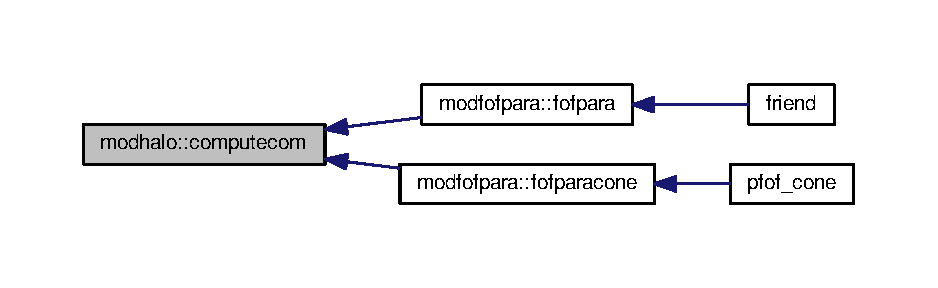
\includegraphics[width=350pt]{classmodhalo_a2f8c1fd1c7fd4704ef7b80cbd4f6272a_icgraph}
\end{center}
\end{figure}


\hypertarget{classmodhalo_a891d00fd31e67d5669ac52117cf13034}{\index{modhalo@{modhalo}!computeradius@{computeradius}}
\index{computeradius@{computeradius}!modhalo@{modhalo}}
\subsubsection[{computeradius}]{\setlength{\rightskip}{0pt plus 5cm}subroutine, public modhalo\-::computeradius (
\begin{DoxyParamCaption}
\item[{logical, intent(in)}]{periodic}
\end{DoxyParamCaption}
)}}\label{classmodhalo_a891d00fd31e67d5669ac52117cf13034}


Definition at line 470 of file modhalo.\-f90.



Here is the caller graph for this function\-:\nopagebreak
\begin{figure}[H]
\begin{center}
\leavevmode
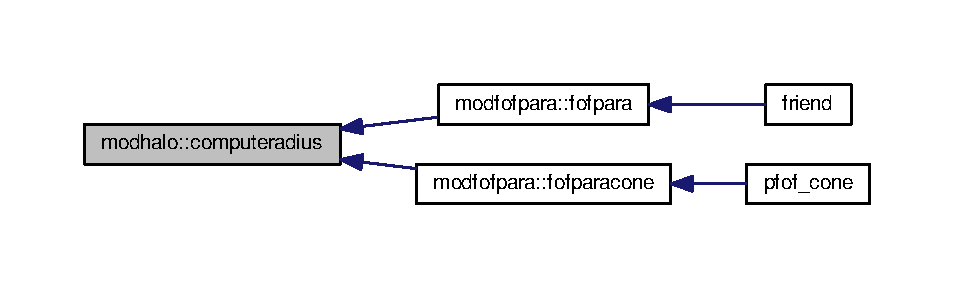
\includegraphics[width=350pt]{classmodhalo_a891d00fd31e67d5669ac52117cf13034_icgraph}
\end{center}
\end{figure}


\hypertarget{classmodhalo_a1ffd35b4853d5d5c196678d253d43ae3}{\index{modhalo@{modhalo}!gatherhaloes@{gatherhaloes}}
\index{gatherhaloes@{gatherhaloes}!modhalo@{modhalo}}
\subsubsection[{gatherhaloes}]{\setlength{\rightskip}{0pt plus 5cm}subroutine, public modhalo\-::gatherhaloes (
\begin{DoxyParamCaption}
\item[{integer, intent(in)}]{mpicomm, }
\item[{class(type\-\_\-parameter\-\_\-pfof), intent(in)}]{param}
\end{DoxyParamCaption}
)}}\label{classmodhalo_a1ffd35b4853d5d5c196678d253d43ae3}


Exchange the particles so that particles belonging to one halo are gathered on the same process. 


\begin{DoxyParams}[1]{Parameters}
\mbox{\tt in}  & {\em mpicomm} & M\-P\-I communicator used for the communications \\
\hline
\end{DoxyParams}


Definition at line 59 of file modhalo.\-f90.



References modmpicommons\-::emergencystop().



Here is the call graph for this function\-:\nopagebreak
\begin{figure}[H]
\begin{center}
\leavevmode
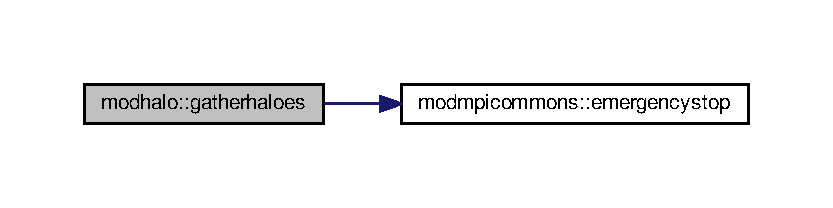
\includegraphics[width=350pt]{classmodhalo_a1ffd35b4853d5d5c196678d253d43ae3_cgraph}
\end{center}
\end{figure}




Here is the caller graph for this function\-:\nopagebreak
\begin{figure}[H]
\begin{center}
\leavevmode
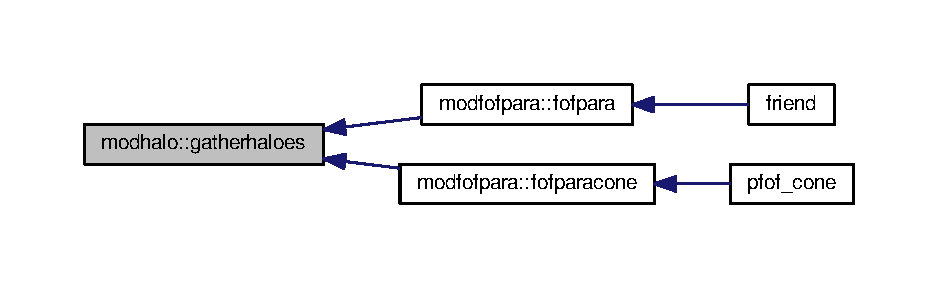
\includegraphics[width=350pt]{classmodhalo_a1ffd35b4853d5d5c196678d253d43ae3_icgraph}
\end{center}
\end{figure}


\hypertarget{classmodhalo_ac468bdd056bc7c1db7e5338bce89ed5b}{\index{modhalo@{modhalo}!selecthaloes@{selecthaloes}}
\index{selecthaloes@{selecthaloes}!modhalo@{modhalo}}
\subsubsection[{selecthaloes}]{\setlength{\rightskip}{0pt plus 5cm}subroutine, public modhalo\-::selecthaloes (
\begin{DoxyParamCaption}
\item[{class(type\-\_\-parameter\-\_\-pfof), intent(in)}]{param}
\end{DoxyParamCaption}
)}}\label{classmodhalo_ac468bdd056bc7c1db7e5338bce89ed5b}


Definition at line 278 of file modhalo.\-f90.



Here is the caller graph for this function\-:\nopagebreak
\begin{figure}[H]
\begin{center}
\leavevmode
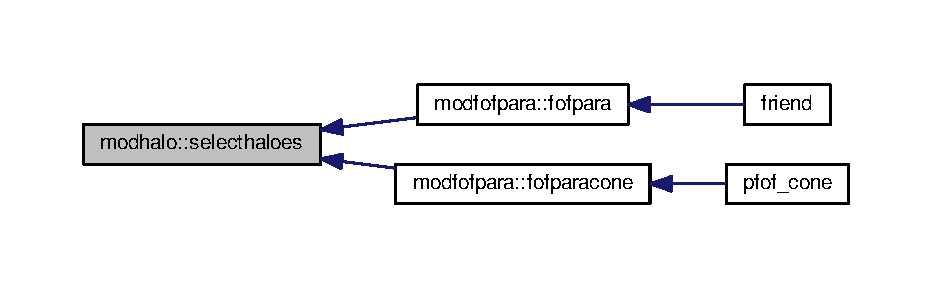
\includegraphics[width=350pt]{classmodhalo_ac468bdd056bc7c1db7e5338bce89ed5b_icgraph}
\end{center}
\end{figure}




\subsection{Member Data Documentation}
\hypertarget{classmodhalo_aea1cd3a6f28ec75795cb930326cc2744}{\index{modhalo@{modhalo}!final\-\_\-local\-\_\-npart@{final\-\_\-local\-\_\-npart}}
\index{final\-\_\-local\-\_\-npart@{final\-\_\-local\-\_\-npart}!modhalo@{modhalo}}
\subsubsection[{final\-\_\-local\-\_\-npart}]{\setlength{\rightskip}{0pt plus 5cm}integer(kind=4), public modhalo\-::final\-\_\-local\-\_\-npart}}\label{classmodhalo_aea1cd3a6f28ec75795cb930326cc2744}


number of particles after the particles have been exchanged to gather them by haloes 



Definition at line 17 of file modhalo.\-f90.

\hypertarget{classmodhalo_afbee38374bfcb2e59a2a9012bf9e1ac6}{\index{modhalo@{modhalo}!halocompos@{halocompos}}
\index{halocompos@{halocompos}!modhalo@{modhalo}}
\subsubsection[{halocompos}]{\setlength{\rightskip}{0pt plus 5cm}real(kind=8), dimension(\-:,\-:), allocatable, public modhalo\-::halocompos}}\label{classmodhalo_afbee38374bfcb2e59a2a9012bf9e1ac6}


position of the center of mass of each halo 



Definition at line 28 of file modhalo.\-f90.

\hypertarget{classmodhalo_acf8ec6b80c5836d34bf47531c2815ce9}{\index{modhalo@{modhalo}!halocomvel@{halocomvel}}
\index{halocomvel@{halocomvel}!modhalo@{modhalo}}
\subsubsection[{halocomvel}]{\setlength{\rightskip}{0pt plus 5cm}real(kind=8), dimension(\-:,\-:), allocatable, public modhalo\-::halocomvel}}\label{classmodhalo_acf8ec6b80c5836d34bf47531c2815ce9}


velocity of the center of mass of each halo 



Definition at line 29 of file modhalo.\-f90.

\hypertarget{classmodhalo_a123a9c168d495f9bbe3d1e25be025105}{\index{modhalo@{modhalo}!haloid@{haloid}}
\index{haloid@{haloid}!modhalo@{modhalo}}
\subsubsection[{haloid}]{\setlength{\rightskip}{0pt plus 5cm}integer(kind=pri), dimension(\-:), allocatable, public modhalo\-::haloid}}\label{classmodhalo_a123a9c168d495f9bbe3d1e25be025105}


I\-D of the haloes. 



Definition at line 19 of file modhalo.\-f90.

\hypertarget{classmodhalo_ad235215a443e0871d790576ff1ad77c2}{\index{modhalo@{modhalo}!halomass@{halomass}}
\index{halomass@{halomass}!modhalo@{modhalo}}
\subsubsection[{halomass}]{\setlength{\rightskip}{0pt plus 5cm}integer(kind=4), dimension(\-:), allocatable, public modhalo\-::halomass}}\label{classmodhalo_ad235215a443e0871d790576ff1ad77c2}


mass of the haloes 



Definition at line 18 of file modhalo.\-f90.

\hypertarget{classmodhalo_aa38fb84fd13087a625a48555740b9f2d}{\index{modhalo@{modhalo}!halonb@{halonb}}
\index{halonb@{halonb}!modhalo@{modhalo}}
\subsubsection[{halonb}]{\setlength{\rightskip}{0pt plus 5cm}integer(kind=4), public modhalo\-::halonb}}\label{classmodhalo_aa38fb84fd13087a625a48555740b9f2d}


local number of haloes 



Definition at line 14 of file modhalo.\-f90.

\hypertarget{classmodhalo_ad416ab5cda1e3a837e8392415f305ffd}{\index{modhalo@{modhalo}!halonb\-\_\-all@{halonb\-\_\-all}}
\index{halonb\-\_\-all@{halonb\-\_\-all}!modhalo@{modhalo}}
\subsubsection[{halonb\-\_\-all}]{\setlength{\rightskip}{0pt plus 5cm}integer(kind=4), public modhalo\-::halonb\-\_\-all}}\label{classmodhalo_ad416ab5cda1e3a837e8392415f305ffd}


global number of haloes 



Definition at line 15 of file modhalo.\-f90.

\hypertarget{classmodhalo_af8ef97601340370e842fce756e116863}{\index{modhalo@{modhalo}!halopartfor@{halopartfor}}
\index{halopartfor@{halopartfor}!modhalo@{modhalo}}
\subsubsection[{halopartfor}]{\setlength{\rightskip}{0pt plus 5cm}real(kind=4), dimension(\-:,\-:), allocatable, public modhalo\-::halopartfor}}\label{classmodhalo_af8ef97601340370e842fce756e116863}


force on the particles belonging to one of the local haloes 



Definition at line 27 of file modhalo.\-f90.

\hypertarget{classmodhalo_a2355dfa04d7ba9d48277d3f4d1e44a64}{\index{modhalo@{modhalo}!halopartid@{halopartid}}
\index{halopartid@{halopartid}!modhalo@{modhalo}}
\subsubsection[{halopartid}]{\setlength{\rightskip}{0pt plus 5cm}integer(kind=pri), dimension(\-:), allocatable, public modhalo\-::halopartid}}\label{classmodhalo_a2355dfa04d7ba9d48277d3f4d1e44a64}


I\-D of the particles belonging to a halo. 



Definition at line 20 of file modhalo.\-f90.

\hypertarget{classmodhalo_aa2c5c12e5bd7198d5571d7ff832ffa38}{\index{modhalo@{modhalo}!halopartnb@{halopartnb}}
\index{halopartnb@{halopartnb}!modhalo@{modhalo}}
\subsubsection[{halopartnb}]{\setlength{\rightskip}{0pt plus 5cm}integer(kind=4), public modhalo\-::halopartnb}}\label{classmodhalo_aa2c5c12e5bd7198d5571d7ff832ffa38}


number of particles belonging to one of the local haloes 



Definition at line 16 of file modhalo.\-f90.

\hypertarget{classmodhalo_a92a746382aef848ff806f8eead8ca9e5}{\index{modhalo@{modhalo}!halopartpos@{halopartpos}}
\index{halopartpos@{halopartpos}!modhalo@{modhalo}}
\subsubsection[{halopartpos}]{\setlength{\rightskip}{0pt plus 5cm}real(kind=4), dimension(\-:,\-:), allocatable, public modhalo\-::halopartpos}}\label{classmodhalo_a92a746382aef848ff806f8eead8ca9e5}


position of the particles belonging to one of the local haloes 



Definition at line 24 of file modhalo.\-f90.

\hypertarget{classmodhalo_a5d7a2e398703c4b5e5826d4e80638f6b}{\index{modhalo@{modhalo}!halopartpot@{halopartpot}}
\index{halopartpot@{halopartpot}!modhalo@{modhalo}}
\subsubsection[{halopartpot}]{\setlength{\rightskip}{0pt plus 5cm}real(kind=4), dimension(\-:), allocatable, public modhalo\-::halopartpot}}\label{classmodhalo_a5d7a2e398703c4b5e5826d4e80638f6b}


potential of the particles belonging to one of the local haloes 



Definition at line 26 of file modhalo.\-f90.

\hypertarget{classmodhalo_a3c78e77057ed6c209d4081c8d559aed3}{\index{modhalo@{modhalo}!halopartramsesid@{halopartramsesid}}
\index{halopartramsesid@{halopartramsesid}!modhalo@{modhalo}}
\subsubsection[{halopartramsesid}]{\setlength{\rightskip}{0pt plus 5cm}integer(kind=pri), dimension(\-:), allocatable, public modhalo\-::halopartramsesid}}\label{classmodhalo_a3c78e77057ed6c209d4081c8d559aed3}


R\-A\-M\-S\-E\-S I\-D of the particles belonging to a halo, used only for lightcone halo. 



Definition at line 21 of file modhalo.\-f90.

\hypertarget{classmodhalo_abd1eee90e1638db519b34633410ff9d1}{\index{modhalo@{modhalo}!halopartvel@{halopartvel}}
\index{halopartvel@{halopartvel}!modhalo@{modhalo}}
\subsubsection[{halopartvel}]{\setlength{\rightskip}{0pt plus 5cm}real(kind=4), dimension(\-:,\-:), allocatable, public modhalo\-::halopartvel}}\label{classmodhalo_abd1eee90e1638db519b34633410ff9d1}


velocity of the particles belonging to one of the local haloes 



Definition at line 25 of file modhalo.\-f90.

\hypertarget{classmodhalo_ace49f47effa6d6b9bfbb88aaca6bc0ee}{\index{modhalo@{modhalo}!haloradius@{haloradius}}
\index{haloradius@{haloradius}!modhalo@{modhalo}}
\subsubsection[{haloradius}]{\setlength{\rightskip}{0pt plus 5cm}real(kind=8), dimension(\-:), allocatable, public modhalo\-::haloradius}}\label{classmodhalo_ace49f47effa6d6b9bfbb88aaca6bc0ee}


radius of each halo 



Definition at line 30 of file modhalo.\-f90.

\hypertarget{classmodhalo_a5dfc215badbd6aa90e9330266a673923}{\index{modhalo@{modhalo}!halosubhalonb@{halosubhalonb}}
\index{halosubhalonb@{halosubhalonb}!modhalo@{modhalo}}
\subsubsection[{halosubhalonb}]{\setlength{\rightskip}{0pt plus 5cm}integer(kind=4), dimension(\-:), allocatable, public modhalo\-::halosubhalonb}}\label{classmodhalo_a5dfc215badbd6aa90e9330266a673923}


number of subhalo for each halo 



Definition at line 22 of file modhalo.\-f90.



The documentation for this module was generated from the following file\-:\begin{DoxyCompactItemize}
\item 
/home/roy/\-Travail/\-Devel/\-Cosmologie/\-Pfof/branches/\-Modif\-Struct/common/src/\hyperlink{modhalo_8f90}{modhalo.\-f90}\end{DoxyCompactItemize}

\hypertarget{classmodhdf5}{\section{modhdf5 Module Reference}
\label{classmodhdf5}\index{modhdf5@{modhdf5}}
}


This module contains wrappers for H\-D\-F5 serial and M\-P\-I I/\-O functions.  


\subsection*{Data Types}
\begin{DoxyCompactItemize}
\item 
interface \hyperlink{interfacemodhdf5_1_1hdf5__read__attr}{hdf5\-\_\-read\-\_\-attr}
\begin{DoxyCompactList}\small\item\em Generic inteface used to read attributes from a hdf5 file. \end{DoxyCompactList}\item 
interface \hyperlink{interfacemodhdf5_1_1hdf5__read__data}{hdf5\-\_\-read\-\_\-data}
\begin{DoxyCompactList}\small\item\em Generic inteface used to read data from a hdf5 file. \end{DoxyCompactList}\item 
interface \hyperlink{interfacemodhdf5_1_1hdf5__read__mpi__data}{hdf5\-\_\-read\-\_\-mpi\-\_\-data}
\begin{DoxyCompactList}\small\item\em Generic inteface used to read data from a parallel hdf5 file. \end{DoxyCompactList}\item 
interface \hyperlink{interfacemodhdf5_1_1hdf5__write__attr}{hdf5\-\_\-write\-\_\-attr}
\begin{DoxyCompactList}\small\item\em Generic inteface used to write attributes in a hdf5 file. \end{DoxyCompactList}\item 
interface \hyperlink{interfacemodhdf5_1_1hdf5__write__data}{hdf5\-\_\-write\-\_\-data}
\begin{DoxyCompactList}\small\item\em Generic inteface used to write data in a hdf5 file. \end{DoxyCompactList}\item 
interface \hyperlink{interfacemodhdf5_1_1hdf5__write__mpi__data}{hdf5\-\_\-write\-\_\-mpi\-\_\-data}
\begin{DoxyCompactList}\small\item\em Generic inteface used to write data in a parallel hdf5 file. \end{DoxyCompactList}\end{DoxyCompactItemize}
\subsection*{Public Member Functions}
\begin{DoxyCompactItemize}
\item 
subroutine, public \hyperlink{classmodhdf5_a78ec7a0bfdcd60f1ce1ecf0c88bb7cd9}{hdf5\-\_\-init} ()
\begin{DoxyCompactList}\small\item\em Open the hdf5 interface. \end{DoxyCompactList}\item 
subroutine, public \hyperlink{classmodhdf5_ace643e6a3e592dbe1be4d158888eb477}{hdf5\-\_\-finalize} ()
\begin{DoxyCompactList}\small\item\em Close the hdf5 interface. \end{DoxyCompactList}\item 
subroutine, public \hyperlink{classmodhdf5_a11539d06d180bff29d3c56ba198451d4}{hdf5\-\_\-open\-\_\-file} (filename, file\-\_\-id)
\begin{DoxyCompactList}\small\item\em Open an existing hdf5 file. \end{DoxyCompactList}\item 
subroutine, public \hyperlink{classmodhdf5_a9f6976ee158485f6b203635df23156e3}{hdf5\-\_\-open\-\_\-mpi\-\_\-file} (filename, comm, file\-\_\-id)
\begin{DoxyCompactList}\small\item\em Open an existing 'parallel' hdf5 file shared by the communicator comm. \end{DoxyCompactList}\item 
subroutine, public \hyperlink{classmodhdf5_aba50f37e2c24ac3271cdfc8877ebdcd9}{hdf5\-\_\-create\-\_\-mpi\-\_\-file} (filename, comm, file\-\_\-id)
\begin{DoxyCompactList}\small\item\em Create and open a 'parallel' hdf5 file shared by the communicator comm. \end{DoxyCompactList}\item 
subroutine, public \hyperlink{classmodhdf5_a72cb805582425e8633c70c5db85df8bc}{hdf5\-\_\-close\-\_\-mpi\-\_\-file} (file\-\_\-id)
\begin{DoxyCompactList}\small\item\em Close a 'parallel' hdf5 file. \end{DoxyCompactList}\item 
subroutine, public \hyperlink{classmodhdf5_a66cf3f318aafac811c2422f8155f7ae1}{hdf5\-\_\-create\-\_\-file} (filename, file\-\_\-id)
\begin{DoxyCompactList}\small\item\em Create and open a hdf5 file. \end{DoxyCompactList}\item 
subroutine, public \hyperlink{classmodhdf5_af70ee678ccdc5ce829431ebe909264a9}{hdf5\-\_\-close\-\_\-file} (file\-\_\-id)
\begin{DoxyCompactList}\small\item\em Close a h5 file. \end{DoxyCompactList}\item 
subroutine, public \hyperlink{classmodhdf5_ae547666d0167e2a78d6529e11c1faa92}{hdf5\-\_\-open\-\_\-group} (id, name, group\-\_\-id)
\begin{DoxyCompactList}\small\item\em Open an existing hdf5 group. \end{DoxyCompactList}\item 
subroutine, public \hyperlink{classmodhdf5_a5486f9c861f7b8ee2060015acf0169a4}{hdf5\-\_\-create\-\_\-group} (id, name, group\-\_\-id)
\begin{DoxyCompactList}\small\item\em Create and open a hdf5 group. \end{DoxyCompactList}\item 
subroutine, public \hyperlink{classmodhdf5_aba547bfdd3dc38385069b0885ab5d526}{hdf5\-\_\-close\-\_\-group} (group\-\_\-id)
\begin{DoxyCompactList}\small\item\em Close a hdf5 group. \end{DoxyCompactList}\end{DoxyCompactItemize}
\subsection*{Public Attributes}
\begin{DoxyCompactItemize}
\item 
integer(kind=4), parameter, public \hyperlink{classmodhdf5_a74fed11716b5063ece33a584a5872f7a}{h5strlen} = 32
\end{DoxyCompactItemize}
\subsection*{Private Member Functions}
\begin{DoxyCompactItemize}
\item 
subroutine \hyperlink{classmodhdf5_a85487dfda18b03bd8b48100b016240b3}{hdf5\-\_\-write\-\_\-int4\-\_\-1d} (id, name, n1, data)
\begin{DoxyCompactList}\small\item\em Write a 1-\/\-D integer(kind=4) array in a serial file. \end{DoxyCompactList}\item 
subroutine \hyperlink{classmodhdf5_ac1a8b8e5ce7ef658ba72dab5853a855a}{hdf5\-\_\-write\-\_\-int8\-\_\-0d} (id, name, data)
\begin{DoxyCompactList}\small\item\em Write an integer(kind=8) scalar in a serial file. \end{DoxyCompactList}\item 
subroutine \hyperlink{classmodhdf5_af39615b3539b84afc3890884aafec217}{hdf5\-\_\-write\-\_\-int8\-\_\-1d} (id, name, n1, data)
\begin{DoxyCompactList}\small\item\em Write a 1-\/\-D integer(kind=8) array in a serial file. \end{DoxyCompactList}\item 
subroutine \hyperlink{classmodhdf5_ab39fa5690f5f029a8beea46dd8030b1d}{hdf5\-\_\-write\-\_\-int4\-\_\-2d} (id, name, n1, n2, data)
\begin{DoxyCompactList}\small\item\em Write a 2-\/\-D integer(kind=4) array in a serial file. \end{DoxyCompactList}\item 
subroutine \hyperlink{classmodhdf5_abcc24e701a795a92f16c6d4c1eb034c7}{hdf5\-\_\-write\-\_\-int8\-\_\-2d} (id, name, n1, n2, data)
\begin{DoxyCompactList}\small\item\em Write a 2-\/\-D integer(kind=8) array in a serial file. \end{DoxyCompactList}\item 
subroutine \hyperlink{classmodhdf5_a5f075a274076e480eee835fd3b9573af}{hdf5\-\_\-write\-\_\-real4\-\_\-1d} (id, name, n1, data)
\begin{DoxyCompactList}\small\item\em Write a 1-\/\-D real(kind=4) array in a serial file. \end{DoxyCompactList}\item 
subroutine \hyperlink{classmodhdf5_aed41c10954f7cb054d46df0c012d147d}{hdf5\-\_\-write\-\_\-real8\-\_\-1d} (id, name, n1, data)
\begin{DoxyCompactList}\small\item\em Write a 1-\/\-D real(kind=8) array in a serial file. \end{DoxyCompactList}\item 
subroutine \hyperlink{classmodhdf5_a71a612d3c6bc8959576fe46d7bab679f}{hdf5\-\_\-write\-\_\-real4\-\_\-2d} (id, name, n1, n2, data)
\begin{DoxyCompactList}\small\item\em Write a 2-\/\-D real(kind=4) array in a serial file. \end{DoxyCompactList}\item 
subroutine \hyperlink{classmodhdf5_a86d263896481bcb679282cede10ab4a1}{hdf5\-\_\-write\-\_\-real8\-\_\-2d} (id, name, n1, n2, data)
\begin{DoxyCompactList}\small\item\em Write a 2-\/\-D real(kind=8) array in a serial file. \end{DoxyCompactList}\item 
subroutine \hyperlink{classmodhdf5_af38c097f92a373ed47962ec1e02f4cb3}{hdf5\-\_\-write\-\_\-mpi\-\_\-int4\-\_\-1d} (id, name, n1, data, comm, empty)
\begin{DoxyCompactList}\small\item\em Write a 1-\/\-D integer(kind=4) array in a parallel file. \end{DoxyCompactList}\item 
subroutine \hyperlink{classmodhdf5_a727abaf04f522d9a2a2accdbf3512a96}{hdf5\-\_\-write\-\_\-mpi\-\_\-int4\-\_\-2d} (id, name, n1, n2, data, comm, empty)
\begin{DoxyCompactList}\small\item\em Write a 2-\/\-D integer(kind=4) array in a parallel file The array is distributed along the 2nd dimension. \end{DoxyCompactList}\item 
subroutine \hyperlink{classmodhdf5_a3402bae4c5e2b0e315c1728b264798da}{hdf5\-\_\-write\-\_\-mpi\-\_\-int8\-\_\-1d} (id, name, n1, data, comm, empty)
\begin{DoxyCompactList}\small\item\em Write a 1-\/\-D integer(kind=8) array in a parallel file. \end{DoxyCompactList}\item 
subroutine \hyperlink{classmodhdf5_a2ca2e47f5fe959ef8cbf3bdad5bef7f8}{hdf5\-\_\-write\-\_\-mpi\-\_\-int8\-\_\-2d} (id, name, n1, n2, data, comm, empty)
\begin{DoxyCompactList}\small\item\em Write a 2-\/\-D integer(kind=8) array in a parallel file The array is distributed along the 2nd dimension. \end{DoxyCompactList}\item 
subroutine \hyperlink{classmodhdf5_aa5b200799b385418068f6c916bbbad34}{hdf5\-\_\-write\-\_\-mpi\-\_\-real4\-\_\-1d} (id, name, n1, data, comm, empty)
\begin{DoxyCompactList}\small\item\em Write a 1-\/\-D real(kind=4) array in a parallel file. \end{DoxyCompactList}\item 
subroutine \hyperlink{classmodhdf5_a6c880adf75b8b8a5ad56120effed2f6a}{hdf5\-\_\-write\-\_\-mpi\-\_\-real4\-\_\-2d} (id, name, n1, n2, data, comm, empty)
\begin{DoxyCompactList}\small\item\em Write a 2-\/\-D real(kind=4) array in a parallel file The array is distributed along the 2nd dimension. \end{DoxyCompactList}\item 
subroutine \hyperlink{classmodhdf5_a6fe25705d9c64cf43c06c885a71878e2}{hdf5\-\_\-write\-\_\-mpi\-\_\-real8\-\_\-1d} (id, name, n1, data, comm, empty)
\begin{DoxyCompactList}\small\item\em Write a 1-\/\-D real(kind=8) array in a parallel file. \end{DoxyCompactList}\item 
subroutine \hyperlink{classmodhdf5_a670313739a46ec4d9006d8761d35157a}{hdf5\-\_\-write\-\_\-mpi\-\_\-real8\-\_\-2d} (id, name, n1, n2, data, comm, empty)
\begin{DoxyCompactList}\small\item\em Write a 2-\/\-D real(kind=8) array in a parallel file The array is distributed along the 2nd dimension. \end{DoxyCompactList}\item 
subroutine \hyperlink{classmodhdf5_afda2e44922def0d140ce850c12ef2f48}{hdf5\-\_\-read\-\_\-int4\-\_\-1d} (id, name, n1, data)
\begin{DoxyCompactList}\small\item\em Read a 1-\/\-D integer(kind=4) array from a serial file. \end{DoxyCompactList}\item 
subroutine \hyperlink{classmodhdf5_ac60e719f8d357b8ffab4f183a7ca4603}{hdf5\-\_\-read\-\_\-int8\-\_\-0d} (id, name, data)
\begin{DoxyCompactList}\small\item\em Read a 1-\/\-D integer(kind=8) scalar from a serial file. \end{DoxyCompactList}\item 
subroutine \hyperlink{classmodhdf5_a640df6ccea7f28d6ed6b578d8018d7d7}{hdf5\-\_\-read\-\_\-int8\-\_\-1d} (id, name, n1, data)
\begin{DoxyCompactList}\small\item\em Read a 1-\/\-D integer(kind=8) array from a serial file. \end{DoxyCompactList}\item 
subroutine \hyperlink{classmodhdf5_a29f383042b1dc2b1fc1155af48fc98a3}{hdf5\-\_\-read\-\_\-int4\-\_\-2d} (id, name, n1, n2, data)
\begin{DoxyCompactList}\small\item\em Read a 2-\/\-D integer(kind=4) array from a serial file. \end{DoxyCompactList}\item 
subroutine \hyperlink{classmodhdf5_a4ac00fa4fbae4c8a8f936ee48292e114}{hdf5\-\_\-read\-\_\-int8\-\_\-2d} (id, name, n1, n2, data)
\begin{DoxyCompactList}\small\item\em Read a 2-\/\-D integer(kind=8) array from a serial file. \end{DoxyCompactList}\item 
subroutine \hyperlink{classmodhdf5_ae087ad5b47b31640a477e5056aaf97e9}{hdf5\-\_\-read\-\_\-real4\-\_\-1d} (id, name, n1, data)
\begin{DoxyCompactList}\small\item\em Read a 1-\/\-D real(kind=4) array from a serial file. \end{DoxyCompactList}\item 
subroutine \hyperlink{classmodhdf5_a584fb8f065f2c6675049794e856b5085}{hdf5\-\_\-read\-\_\-real8\-\_\-1d} (id, name, n1, data)
\begin{DoxyCompactList}\small\item\em Read a 1-\/\-D real(kind=8) array from a serial file. \end{DoxyCompactList}\item 
subroutine \hyperlink{classmodhdf5_a36acd2df481965d7cb9c1b312fdff7b0}{hdf5\-\_\-read\-\_\-real4\-\_\-2d} (id, name, n1, n2, data)
\begin{DoxyCompactList}\small\item\em Read a 2-\/\-D real(kind=4) array from a serial file. \end{DoxyCompactList}\item 
subroutine \hyperlink{classmodhdf5_a7ba4b99f85945770344cdd73b713ea3a}{hdf5\-\_\-read\-\_\-real8\-\_\-2d} (id, name, n1, n2, data)
\begin{DoxyCompactList}\small\item\em Read a 2-\/\-D real(kind=8) array from a serial file. \end{DoxyCompactList}\item 
subroutine \hyperlink{classmodhdf5_a18b987f7a44198ccc7dd893cbdc322fc}{hdf5\-\_\-read\-\_\-mpi\-\_\-int4\-\_\-1d} (id, name, n1, data, comm)
\begin{DoxyCompactList}\small\item\em Read a 1-\/\-D integer4 array from a parallel file The array is distributed along the 2nd dimension. \end{DoxyCompactList}\item 
subroutine \hyperlink{classmodhdf5_ac96ae5057bcd6745840c716a232d4b66}{hdf5\-\_\-read\-\_\-mpi\-\_\-int4\-\_\-2d} (id, name, n1, n2, data, comm)
\begin{DoxyCompactList}\small\item\em Read a 2-\/\-D integer4 array from a parallel file The array is distributed along the 2nd dimension. \end{DoxyCompactList}\item 
subroutine \hyperlink{classmodhdf5_a2847f70176f88d95e8e6e1bec3a2539e}{hdf5\-\_\-read\-\_\-mpi\-\_\-int8\-\_\-1d} (id, name, n1, data, comm)
\begin{DoxyCompactList}\small\item\em Read a 1-\/\-D integer8 array from a parallel file The array is distributed along the 2nd dimension. \end{DoxyCompactList}\item 
subroutine \hyperlink{classmodhdf5_a41bc63b78ce861c9898ef45642514a9d}{hdf5\-\_\-read\-\_\-mpi\-\_\-int8\-\_\-2d} (id, name, n1, n2, data, comm)
\begin{DoxyCompactList}\small\item\em Read a 2-\/\-D integer8 array from a parallel file The array is distributed along the 2nd dimension. \end{DoxyCompactList}\item 
subroutine \hyperlink{classmodhdf5_a7c2f69141e8a85768536e7c8f79f6348}{hdf5\-\_\-read\-\_\-mpi\-\_\-real4\-\_\-1d} (id, name, n1, data, comm)
\begin{DoxyCompactList}\small\item\em Read a 1-\/\-D real4 array from a parallel file The array is distributed along the 2nd dimension. \end{DoxyCompactList}\item 
subroutine \hyperlink{classmodhdf5_a406b07a6320d4dd08a12ca4b8d6b9e9d}{hdf5\-\_\-read\-\_\-mpi\-\_\-real4\-\_\-2d} (id, name, n1, n2, data, comm)
\begin{DoxyCompactList}\small\item\em Read a 2-\/\-D real4 array from a parallel file The array is distributed along the 2nd dimension. \end{DoxyCompactList}\item 
subroutine \hyperlink{classmodhdf5_afaf6a2a85551a1a7e9638d597c39dc32}{hdf5\-\_\-read\-\_\-mpi\-\_\-real8\-\_\-1d} (id, name, n1, data, comm)
\begin{DoxyCompactList}\small\item\em Read a 1-\/\-D real8 array from a parallel file The array is distributed along the 2nd dimension. \end{DoxyCompactList}\item 
subroutine \hyperlink{classmodhdf5_a29c6c1a0c3de14678ed8eebe304b3255}{hdf5\-\_\-read\-\_\-mpi\-\_\-real8\-\_\-2d} (id, name, n1, n2, data, comm)
\begin{DoxyCompactList}\small\item\em Read a 2-\/\-D real8 array from a parallel file The array is distributed along the 2nd dimension. \end{DoxyCompactList}\item 
subroutine \hyperlink{classmodhdf5_a1f5aac5704c10accbb39476926a4a7aa}{hdf5\-\_\-write\-\_\-int4\-\_\-attr0d} (id, name, data)
\begin{DoxyCompactList}\small\item\em Write an integer4 as attribute. \end{DoxyCompactList}\item 
subroutine \hyperlink{classmodhdf5_a41e511ab23277132cad7aa447804eee4}{hdf5\-\_\-write\-\_\-int4\-\_\-attr1d} (id, name, n1, data)
\begin{DoxyCompactList}\small\item\em Write a 1-\/\-D array of integer4 as attribute. \end{DoxyCompactList}\item 
subroutine \hyperlink{classmodhdf5_a902380b589c35be03e33f0ae8ebdc0dc}{hdf5\-\_\-write\-\_\-int4\-\_\-attr2d} (id, name, n1, n2, data)
\item 
subroutine \hyperlink{classmodhdf5_abadf683caad48e7acd96f916246bf778}{hdf5\-\_\-write\-\_\-real4\-\_\-attr0d} (id, name, data)
\begin{DoxyCompactList}\small\item\em Write a real4 as attribute. \end{DoxyCompactList}\item 
subroutine \hyperlink{classmodhdf5_a6158884984b6690aad27d75c6d5f58a7}{hdf5\-\_\-write\-\_\-real4\-\_\-attr1d} (id, name, n1, data)
\begin{DoxyCompactList}\small\item\em Write a 1-\/\-D array of real4 as attribute. \end{DoxyCompactList}\item 
subroutine \hyperlink{classmodhdf5_ad682a858bcaec8fcd21f646d44d76208}{hdf5\-\_\-write\-\_\-real4\-\_\-attr2d} (id, name, n1, n2, data)
\item 
subroutine \hyperlink{classmodhdf5_a28db26cc0b827091ab455d2419c88b10}{hdf5\-\_\-write\-\_\-real8\-\_\-attr0d} (id, name, data)
\begin{DoxyCompactList}\small\item\em Write a real8 as attribute. \end{DoxyCompactList}\item 
subroutine \hyperlink{classmodhdf5_ad55b7cffc861305840d5f160ba6fa1fd}{hdf5\-\_\-write\-\_\-real8\-\_\-attr1d} (id, name, n1, data)
\begin{DoxyCompactList}\small\item\em Write a 1-\/\-D array of real8 as attribute. \end{DoxyCompactList}\item 
subroutine \hyperlink{classmodhdf5_a71ef9213132fb3f757d29f58f9c20966}{hdf5\-\_\-write\-\_\-real8\-\_\-attr2d} (id, name, n1, n2, data)
\item 
subroutine \hyperlink{classmodhdf5_ad6fea34611cf76b56b5143cd182b8484}{hdf5\-\_\-write\-\_\-char\-\_\-attr} (id, name, data)
\begin{DoxyCompactList}\small\item\em Write a string as attribute. \end{DoxyCompactList}\item 
subroutine \hyperlink{classmodhdf5_a10a4b5212d77e52dba2616ba3abb7df1}{hdf5\-\_\-read\-\_\-int4\-\_\-attr0d} (id, name, attr)
\begin{DoxyCompactList}\small\item\em Read an integer4 attribute in a hdf5 file. \end{DoxyCompactList}\item 
subroutine \hyperlink{classmodhdf5_a2ff1b28dd896cc37583e97a52348039f}{hdf5\-\_\-read\-\_\-int4\-\_\-attr1d} (id, name, n1, attr)
\begin{DoxyCompactList}\small\item\em Read a 1-\/\-D integer4 attribute in a hdf5 file. \end{DoxyCompactList}\item 
subroutine \hyperlink{classmodhdf5_a4ca8f47995bf9df5b6c892781c87dd95}{hdf5\-\_\-read\-\_\-int4\-\_\-attr2d} (id, name, n1, n2, attr)
\begin{DoxyCompactList}\small\item\em Read a 2-\/\-D integer4 attribute in a hdf5 file. \end{DoxyCompactList}\item 
subroutine \hyperlink{classmodhdf5_a6cf3b8369d7cbc96e8639439eb7c51ff}{hdf5\-\_\-read\-\_\-real4\-\_\-attr0d} (id, name, attr)
\begin{DoxyCompactList}\small\item\em Read a real4 attribute in a hdf5 file. \end{DoxyCompactList}\item 
subroutine \hyperlink{classmodhdf5_acd7e7ad91ecc73c632ddc76468dbd083}{hdf5\-\_\-read\-\_\-real4\-\_\-attr1d} (id, name, n1, attr)
\begin{DoxyCompactList}\small\item\em Read a 1-\/\-D real4 attribute in a hdf5 file. \end{DoxyCompactList}\item 
subroutine \hyperlink{classmodhdf5_a783cb12e2d85f812c506fff7cc69f37a}{hdf5\-\_\-read\-\_\-real4\-\_\-attr2d} (id, name, n1, n2, attr)
\begin{DoxyCompactList}\small\item\em Read a 2-\/\-D real4 attribute in a hdf5 file. \end{DoxyCompactList}\item 
subroutine \hyperlink{classmodhdf5_ad2a6c1b4f0229be1ac9f4e4eb0556af4}{hdf5\-\_\-read\-\_\-real8\-\_\-attr0d} (id, name, attr)
\begin{DoxyCompactList}\small\item\em Read a real8 attribute in a hdf5 file. \end{DoxyCompactList}\item 
subroutine \hyperlink{classmodhdf5_a5010be0e91c8d56afbd40530b8064d6a}{hdf5\-\_\-read\-\_\-real8\-\_\-attr1d} (id, name, n1, attr)
\begin{DoxyCompactList}\small\item\em Read a 1-\/\-D real8 attribute in a hdf5 file. \end{DoxyCompactList}\item 
subroutine \hyperlink{classmodhdf5_a85144bc1c41d08550379f855b3974507}{hdf5\-\_\-read\-\_\-real8\-\_\-attr2d} (id, name, n1, n2, attr)
\begin{DoxyCompactList}\small\item\em Read a 2-\/\-D real4 attribute in a hdf5 file. \end{DoxyCompactList}\item 
subroutine \hyperlink{classmodhdf5_a2da336bc6d0ebbf1e6d582469b741a63}{hdf5\-\_\-read\-\_\-char\-\_\-attr} (id, name, n1, attr)
\begin{DoxyCompactList}\small\item\em Read string attribute in a hdf5 file. \end{DoxyCompactList}\end{DoxyCompactItemize}
\subsection*{Private Attributes}
\begin{DoxyCompactItemize}
\item 
integer(kind=4) \hyperlink{classmodhdf5_a7c21e772a564aec00e44e46562e9e840}{h5err}
\begin{DoxyCompactList}\small\item\em hdf5 error code \end{DoxyCompactList}\item 
integer(kind=4) \hyperlink{classmodhdf5_a8d55ad41fc659457afec426d7eb3b2e8}{mpierr}
\begin{DoxyCompactList}\small\item\em mpi error code \end{DoxyCompactList}\end{DoxyCompactItemize}


\subsection{Detailed Description}
This module contains wrappers for H\-D\-F5 serial and M\-P\-I I/\-O functions. 

Authors\-: F. Roy 

Definition at line 8 of file modhdf5.\-f90.



\subsection{Member Function/\-Subroutine Documentation}
\hypertarget{classmodhdf5_af70ee678ccdc5ce829431ebe909264a9}{\index{modhdf5@{modhdf5}!hdf5\-\_\-close\-\_\-file@{hdf5\-\_\-close\-\_\-file}}
\index{hdf5\-\_\-close\-\_\-file@{hdf5\-\_\-close\-\_\-file}!modhdf5@{modhdf5}}
\subsubsection[{hdf5\-\_\-close\-\_\-file}]{\setlength{\rightskip}{0pt plus 5cm}subroutine, public modhdf5\-::hdf5\-\_\-close\-\_\-file (
\begin{DoxyParamCaption}
\item[{integer(hid\-\_\-t), intent(in)}]{file\-\_\-id}
\end{DoxyParamCaption}
)}}\label{classmodhdf5_af70ee678ccdc5ce829431ebe909264a9}


Close a h5 file. 


\begin{DoxyParams}[1]{Parameters}
\mbox{\tt in}  & {\em file\-\_\-id} & hdf5 identifier of the file to close \\
\hline
\end{DoxyParams}


Definition at line 447 of file modhdf5.\-f90.



Here is the caller graph for this function\-:\nopagebreak
\begin{figure}[H]
\begin{center}
\leavevmode
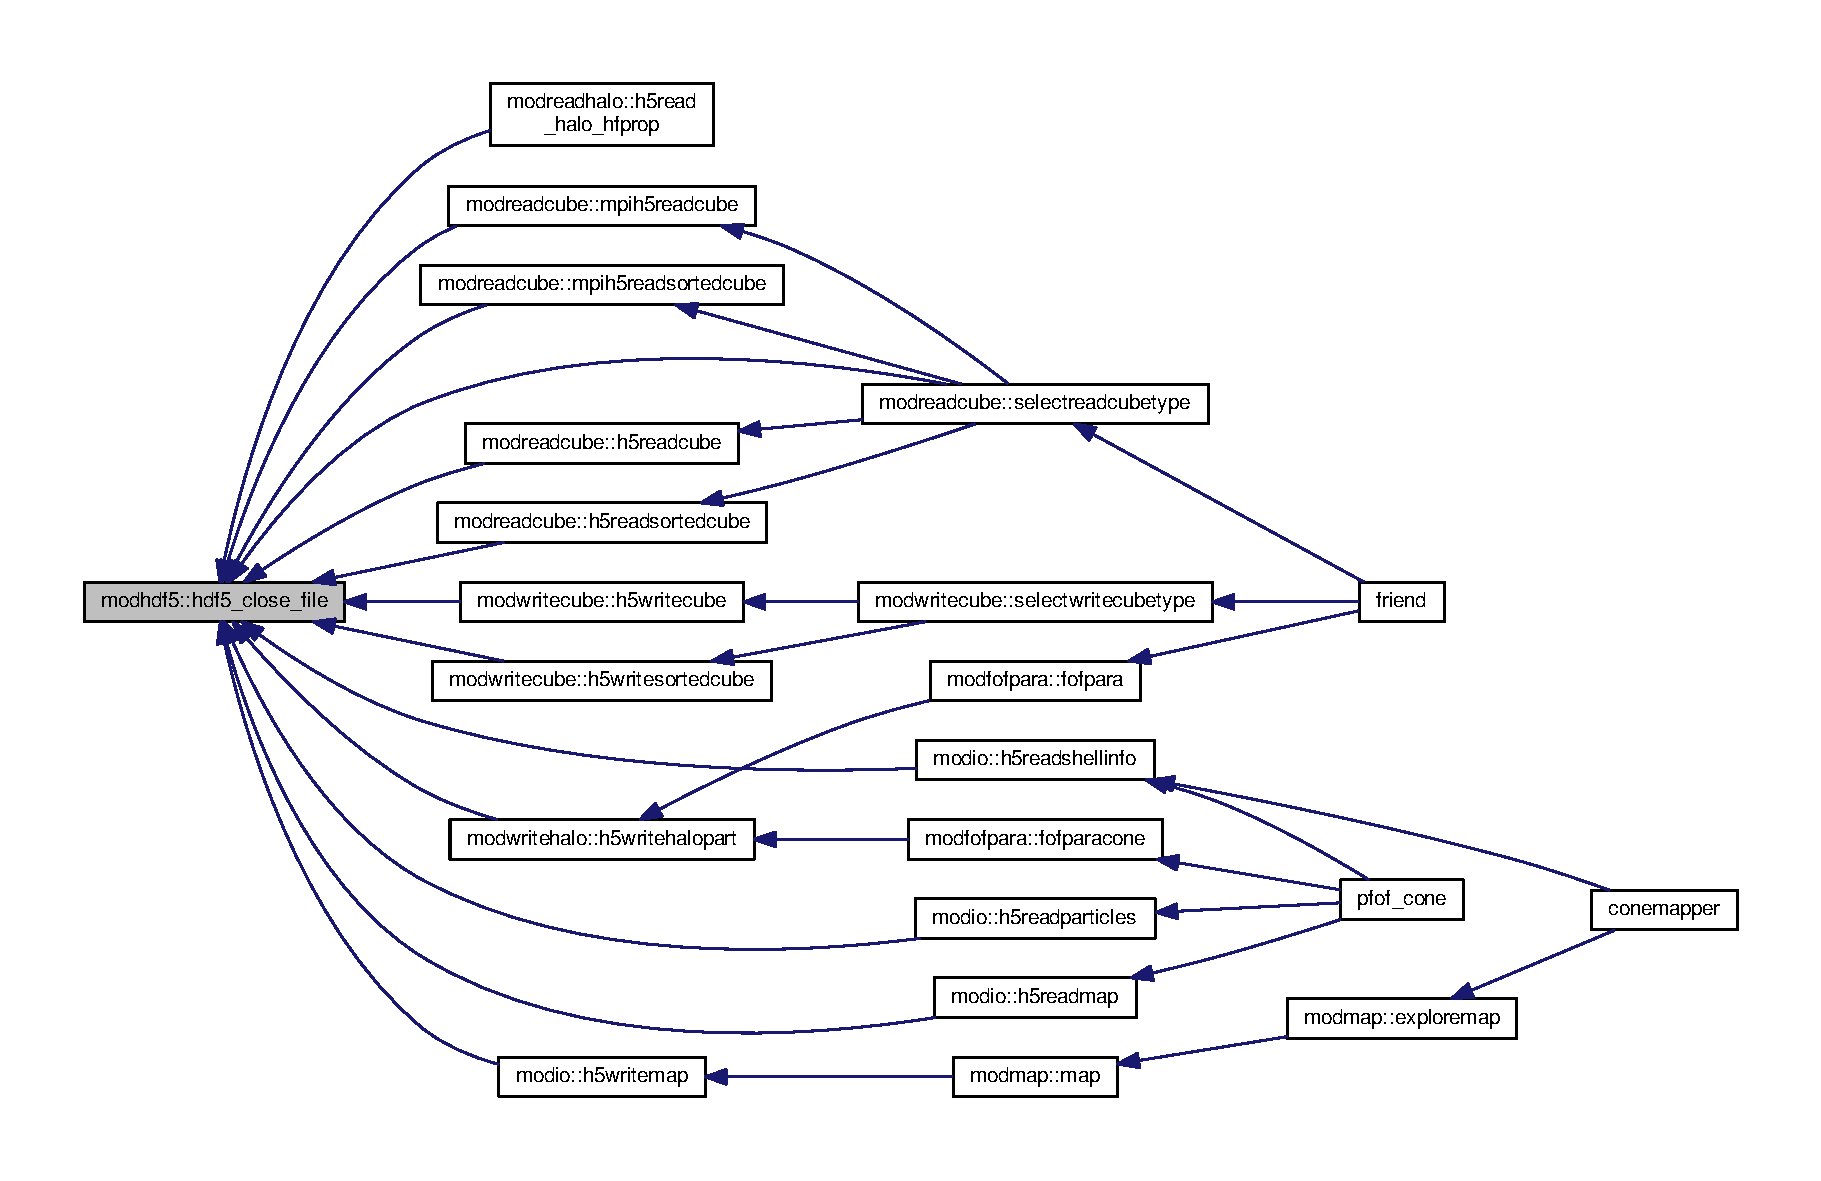
\includegraphics[width=350pt]{classmodhdf5_af70ee678ccdc5ce829431ebe909264a9_icgraph}
\end{center}
\end{figure}


\hypertarget{classmodhdf5_aba547bfdd3dc38385069b0885ab5d526}{\index{modhdf5@{modhdf5}!hdf5\-\_\-close\-\_\-group@{hdf5\-\_\-close\-\_\-group}}
\index{hdf5\-\_\-close\-\_\-group@{hdf5\-\_\-close\-\_\-group}!modhdf5@{modhdf5}}
\subsubsection[{hdf5\-\_\-close\-\_\-group}]{\setlength{\rightskip}{0pt plus 5cm}subroutine, public modhdf5\-::hdf5\-\_\-close\-\_\-group (
\begin{DoxyParamCaption}
\item[{integer(hid\-\_\-t), intent(in)}]{group\-\_\-id}
\end{DoxyParamCaption}
)}}\label{classmodhdf5_aba547bfdd3dc38385069b0885ab5d526}


Close a hdf5 group. 


\begin{DoxyParams}[1]{Parameters}
\mbox{\tt in}  & {\em group\-\_\-id} & group identifier \\
\hline
\end{DoxyParams}


Definition at line 522 of file modhdf5.\-f90.



Here is the caller graph for this function\-:\nopagebreak
\begin{figure}[H]
\begin{center}
\leavevmode
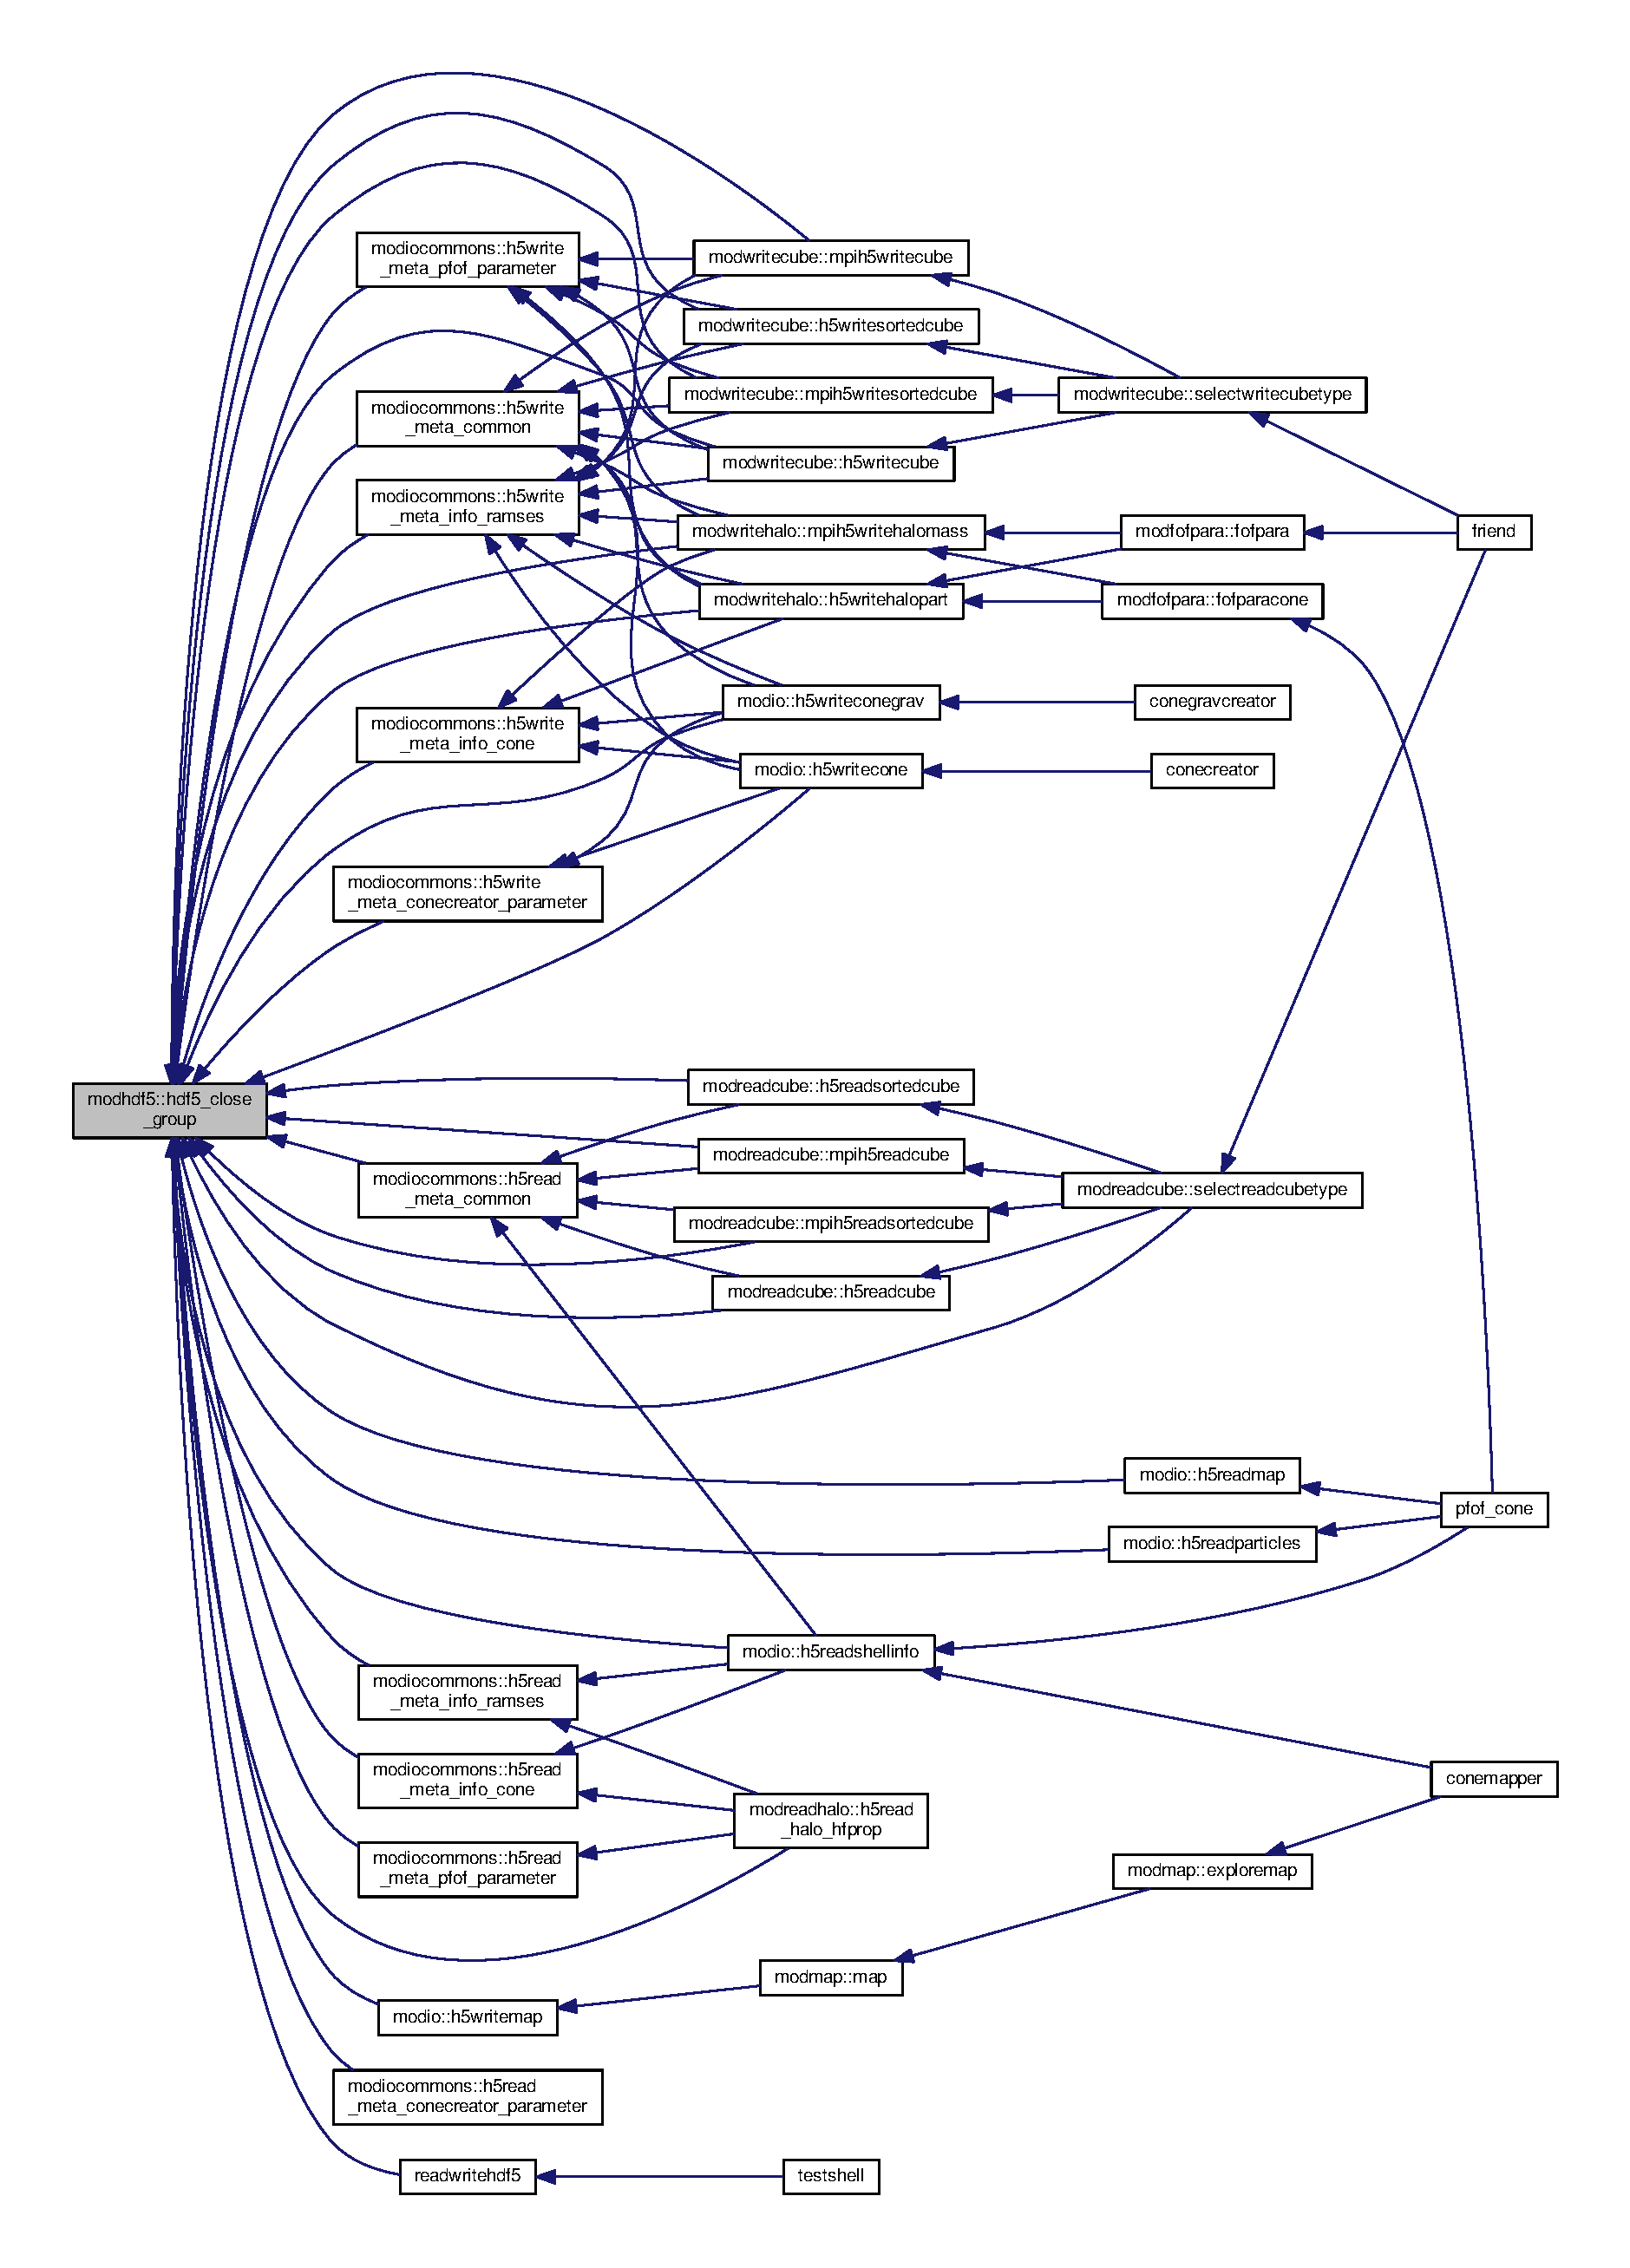
\includegraphics[width=350pt]{classmodhdf5_aba547bfdd3dc38385069b0885ab5d526_icgraph}
\end{center}
\end{figure}


\hypertarget{classmodhdf5_a72cb805582425e8633c70c5db85df8bc}{\index{modhdf5@{modhdf5}!hdf5\-\_\-close\-\_\-mpi\-\_\-file@{hdf5\-\_\-close\-\_\-mpi\-\_\-file}}
\index{hdf5\-\_\-close\-\_\-mpi\-\_\-file@{hdf5\-\_\-close\-\_\-mpi\-\_\-file}!modhdf5@{modhdf5}}
\subsubsection[{hdf5\-\_\-close\-\_\-mpi\-\_\-file}]{\setlength{\rightskip}{0pt plus 5cm}subroutine, public modhdf5\-::hdf5\-\_\-close\-\_\-mpi\-\_\-file (
\begin{DoxyParamCaption}
\item[{integer(hid\-\_\-t), intent(in)}]{file\-\_\-id}
\end{DoxyParamCaption}
)}}\label{classmodhdf5_a72cb805582425e8633c70c5db85df8bc}


Close a 'parallel' hdf5 file. 


\begin{DoxyParams}[1]{Parameters}
\mbox{\tt in}  & {\em file\-\_\-id} & hdf5 identifier of the parallel file to close \\
\hline
\end{DoxyParams}


Definition at line 355 of file modhdf5.\-f90.



Here is the caller graph for this function\-:\nopagebreak
\begin{figure}[H]
\begin{center}
\leavevmode
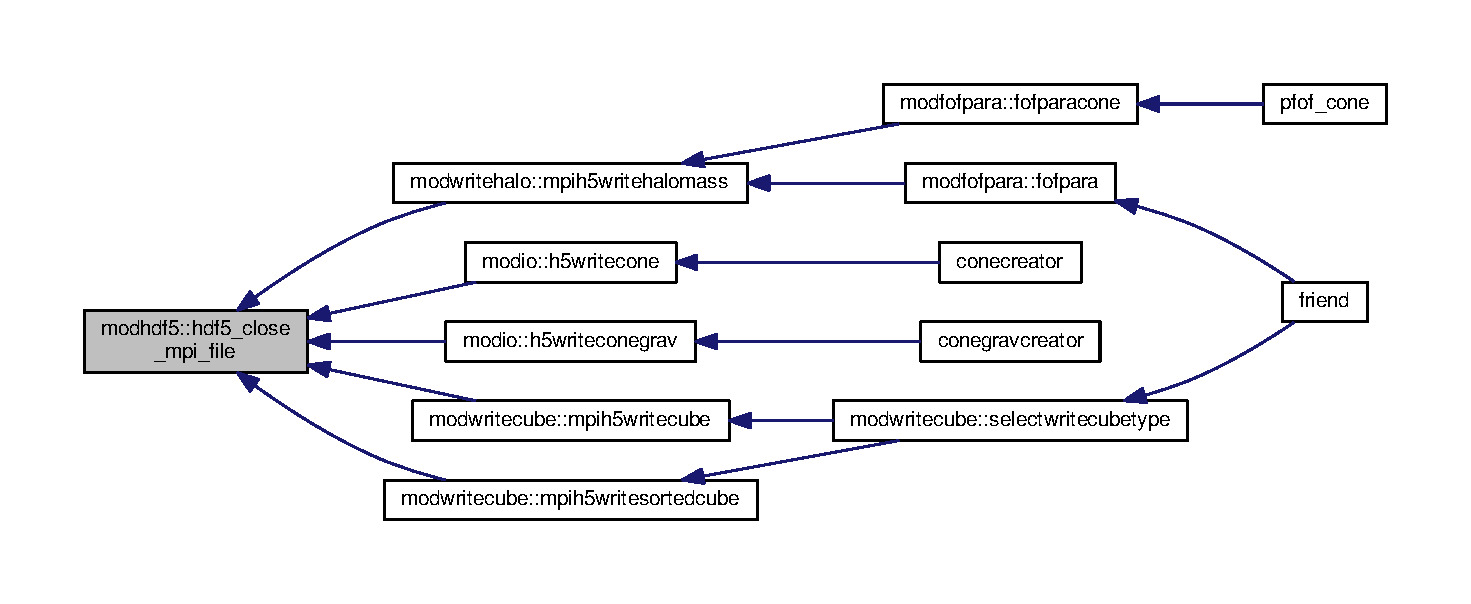
\includegraphics[width=350pt]{classmodhdf5_a72cb805582425e8633c70c5db85df8bc_icgraph}
\end{center}
\end{figure}


\hypertarget{classmodhdf5_a66cf3f318aafac811c2422f8155f7ae1}{\index{modhdf5@{modhdf5}!hdf5\-\_\-create\-\_\-file@{hdf5\-\_\-create\-\_\-file}}
\index{hdf5\-\_\-create\-\_\-file@{hdf5\-\_\-create\-\_\-file}!modhdf5@{modhdf5}}
\subsubsection[{hdf5\-\_\-create\-\_\-file}]{\setlength{\rightskip}{0pt plus 5cm}subroutine, public modhdf5\-::hdf5\-\_\-create\-\_\-file (
\begin{DoxyParamCaption}
\item[{character(len=400), intent(in)}]{filename, }
\item[{integer(hid\-\_\-t), intent(out)}]{file\-\_\-id}
\end{DoxyParamCaption}
)}}\label{classmodhdf5_a66cf3f318aafac811c2422f8155f7ae1}


Create and open a hdf5 file. 


\begin{DoxyParams}[1]{Parameters}
\mbox{\tt in}  & {\em filename} & name of the parallel file to create\\
\hline
\mbox{\tt out}  & {\em file\-\_\-id} & hdf5 identifier of the parallel file \\
\hline
\end{DoxyParams}


Definition at line 376 of file modhdf5.\-f90.



References hdf5\-\_\-create\-\_\-group().



Here is the call graph for this function\-:\nopagebreak
\begin{figure}[H]
\begin{center}
\leavevmode
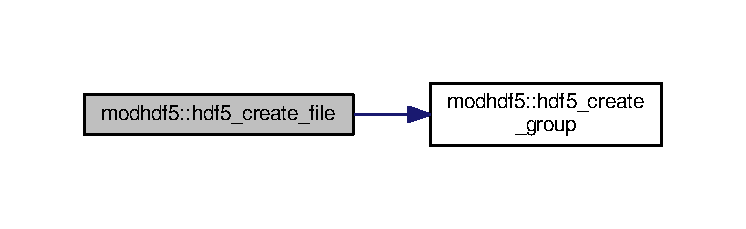
\includegraphics[width=350pt]{classmodhdf5_a66cf3f318aafac811c2422f8155f7ae1_cgraph}
\end{center}
\end{figure}




Here is the caller graph for this function\-:\nopagebreak
\begin{figure}[H]
\begin{center}
\leavevmode
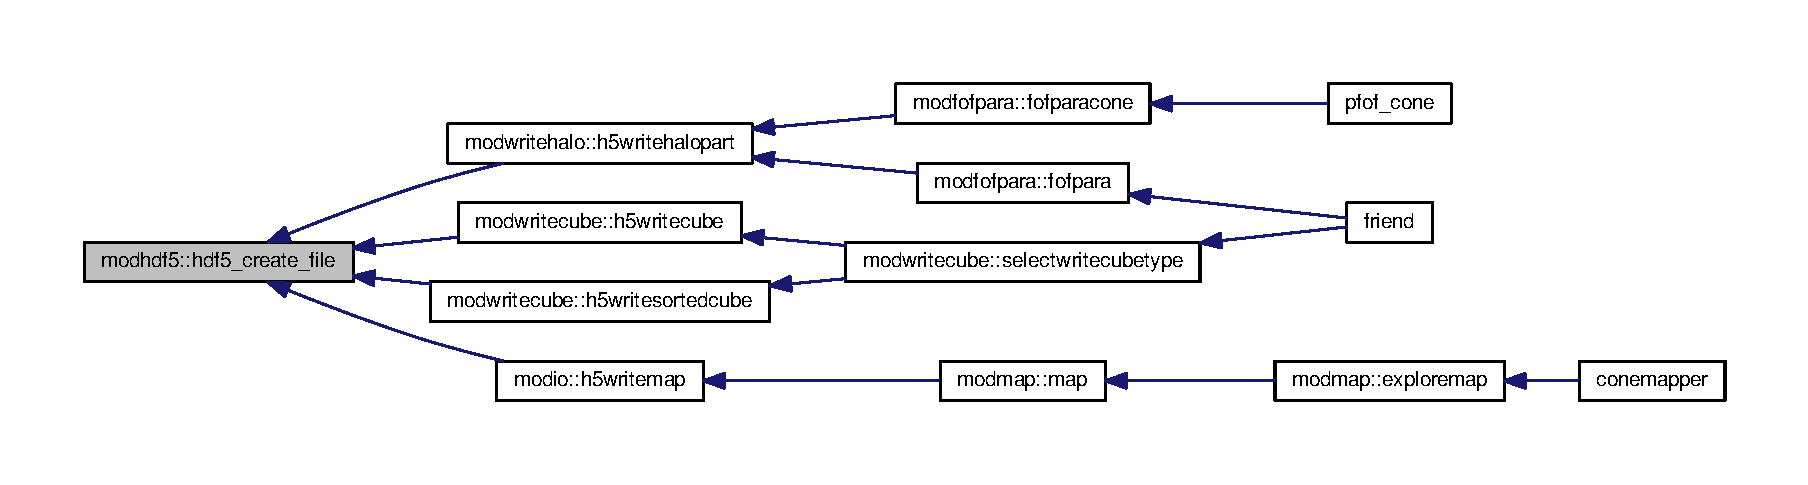
\includegraphics[width=350pt]{classmodhdf5_a66cf3f318aafac811c2422f8155f7ae1_icgraph}
\end{center}
\end{figure}


\hypertarget{classmodhdf5_a5486f9c861f7b8ee2060015acf0169a4}{\index{modhdf5@{modhdf5}!hdf5\-\_\-create\-\_\-group@{hdf5\-\_\-create\-\_\-group}}
\index{hdf5\-\_\-create\-\_\-group@{hdf5\-\_\-create\-\_\-group}!modhdf5@{modhdf5}}
\subsubsection[{hdf5\-\_\-create\-\_\-group}]{\setlength{\rightskip}{0pt plus 5cm}subroutine, public modhdf5\-::hdf5\-\_\-create\-\_\-group (
\begin{DoxyParamCaption}
\item[{integer(hid\-\_\-t), intent(in)}]{id, }
\item[{character(len={\bf h5strlen}), intent(in)}]{name, }
\item[{integer(hid\-\_\-t), intent(out)}]{group\-\_\-id}
\end{DoxyParamCaption}
)}}\label{classmodhdf5_a5486f9c861f7b8ee2060015acf0169a4}


Create and open a hdf5 group. 


\begin{DoxyParams}[1]{Parameters}
\mbox{\tt in}  & {\em id} & \char`\"{}parent\char`\"{} identifier\\
\hline
\mbox{\tt in}  & {\em name} & group name\\
\hline
\mbox{\tt out}  & {\em group\-\_\-id} & group identifier \\
\hline
\end{DoxyParams}


Definition at line 499 of file modhdf5.\-f90.



Here is the caller graph for this function\-:\nopagebreak
\begin{figure}[H]
\begin{center}
\leavevmode
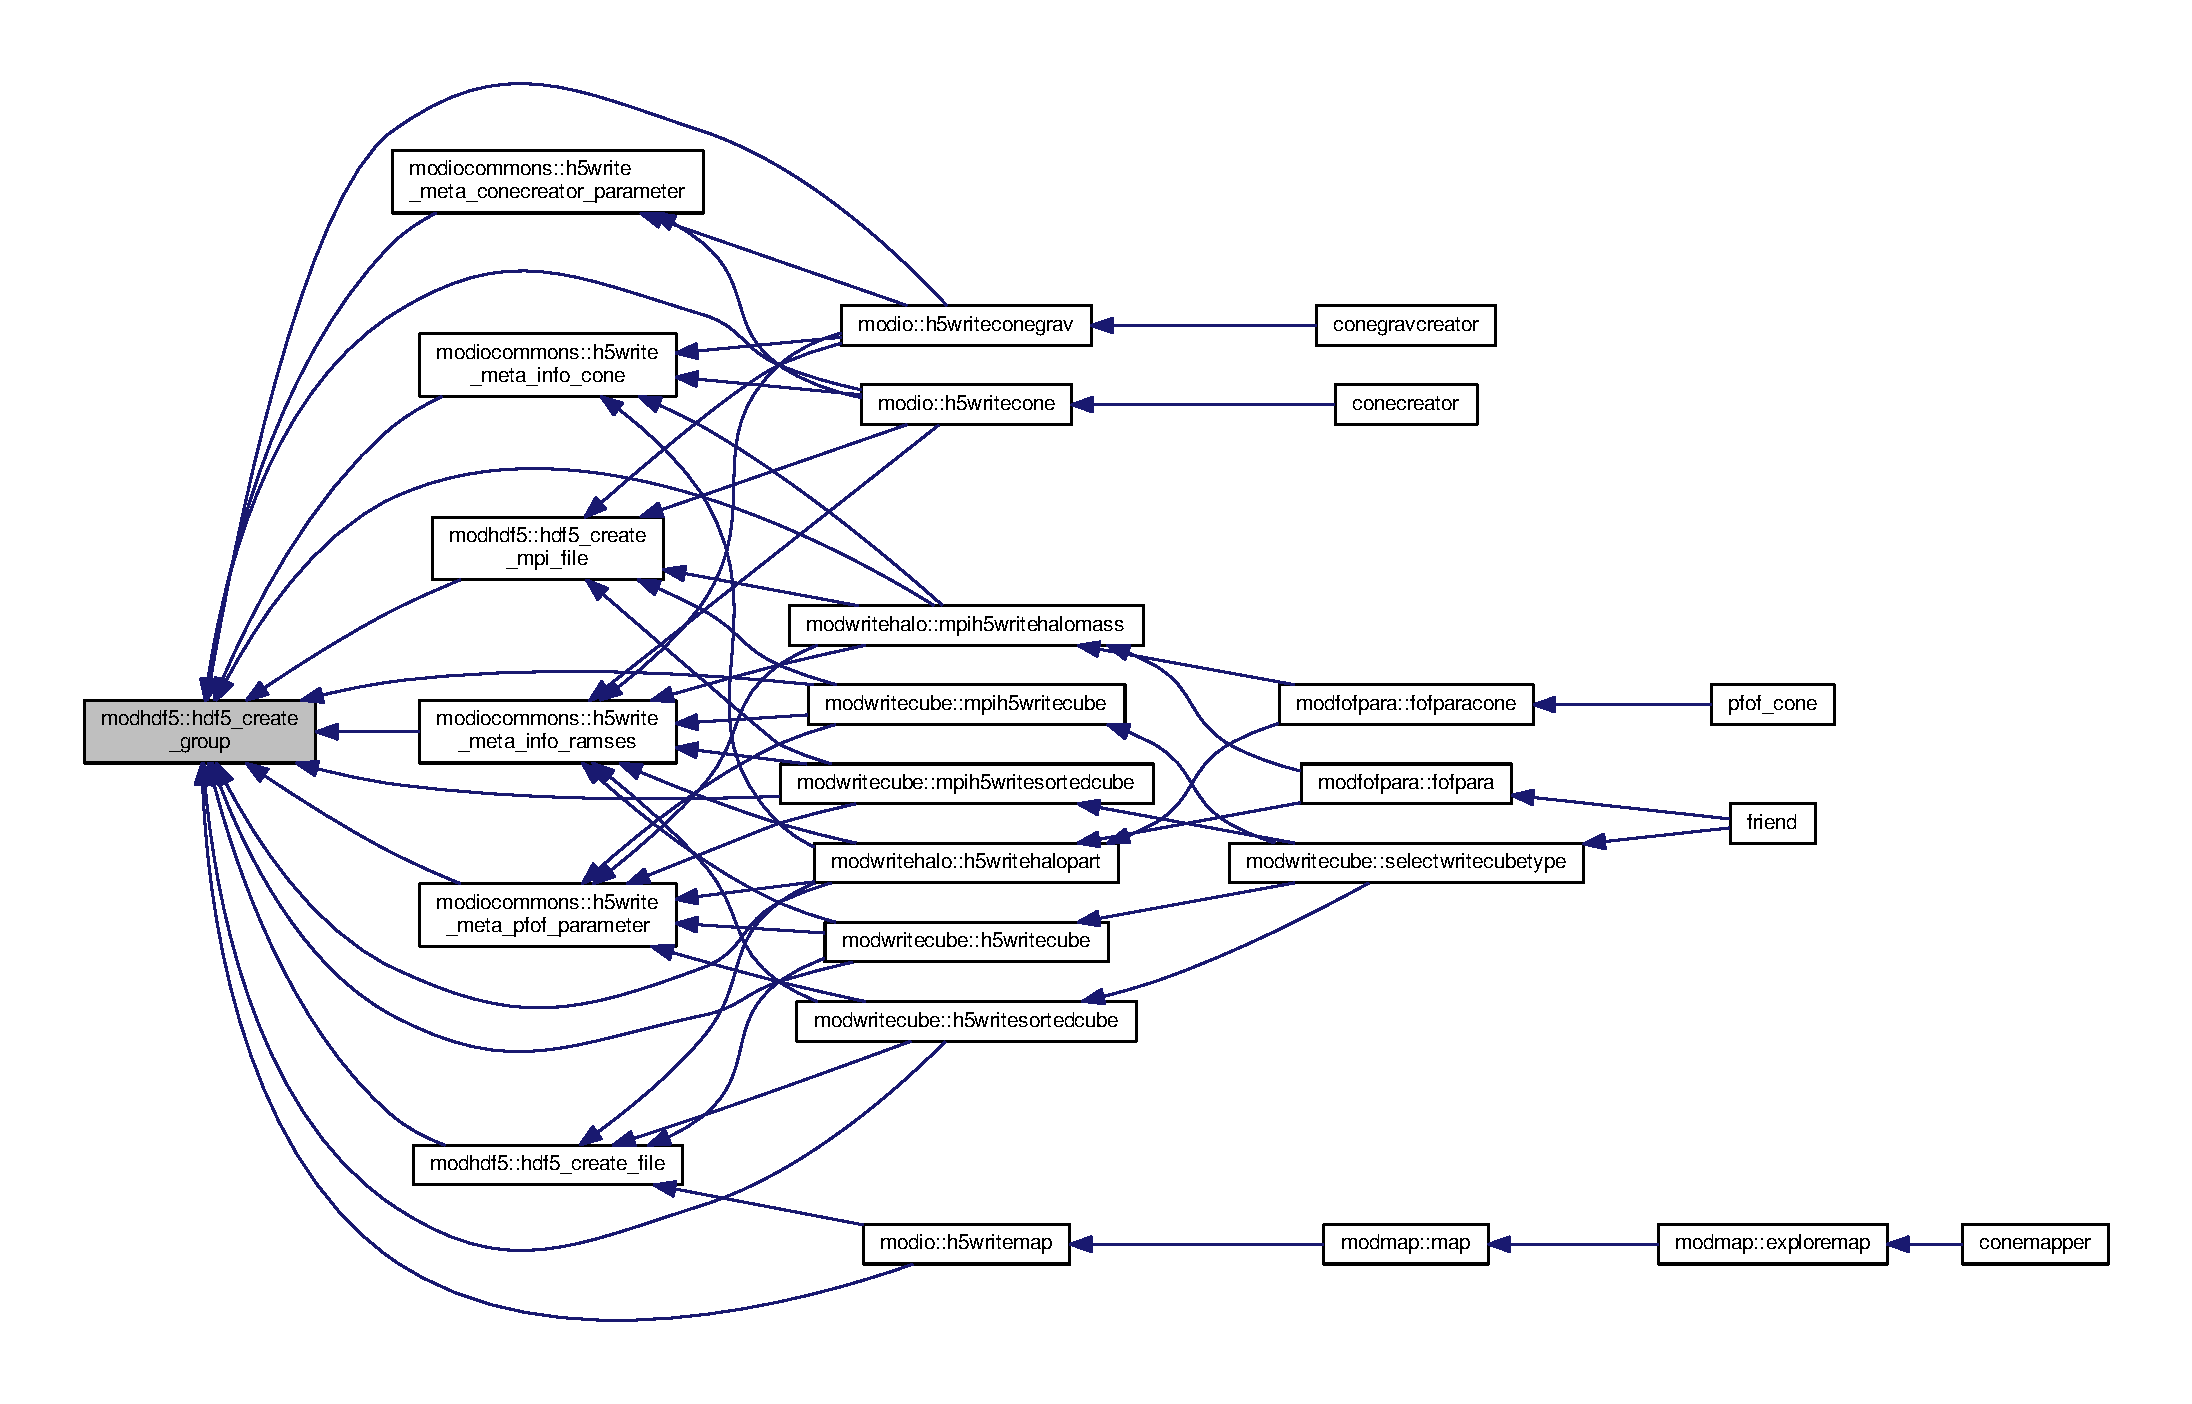
\includegraphics[width=350pt]{classmodhdf5_a5486f9c861f7b8ee2060015acf0169a4_icgraph}
\end{center}
\end{figure}


\hypertarget{classmodhdf5_aba50f37e2c24ac3271cdfc8877ebdcd9}{\index{modhdf5@{modhdf5}!hdf5\-\_\-create\-\_\-mpi\-\_\-file@{hdf5\-\_\-create\-\_\-mpi\-\_\-file}}
\index{hdf5\-\_\-create\-\_\-mpi\-\_\-file@{hdf5\-\_\-create\-\_\-mpi\-\_\-file}!modhdf5@{modhdf5}}
\subsubsection[{hdf5\-\_\-create\-\_\-mpi\-\_\-file}]{\setlength{\rightskip}{0pt plus 5cm}subroutine, public modhdf5\-::hdf5\-\_\-create\-\_\-mpi\-\_\-file (
\begin{DoxyParamCaption}
\item[{character(len=400), intent(in)}]{filename, }
\item[{integer(kind=4), intent(in)}]{comm, }
\item[{integer(hid\-\_\-t), intent(out)}]{file\-\_\-id}
\end{DoxyParamCaption}
)}}\label{classmodhdf5_aba50f37e2c24ac3271cdfc8877ebdcd9}


Create and open a 'parallel' hdf5 file shared by the communicator comm. 


\begin{DoxyParams}[1]{Parameters}
\mbox{\tt in}  & {\em filename} & name of the parallel file to create\\
\hline
\mbox{\tt in}  & {\em comm} & M\-P\-I communicator used for the file access\\
\hline
\mbox{\tt out}  & {\em file\-\_\-id} & hdf5 id of the created file \\
\hline
\end{DoxyParams}


Definition at line 279 of file modhdf5.\-f90.



References hdf5\-\_\-create\-\_\-group().



Here is the call graph for this function\-:\nopagebreak
\begin{figure}[H]
\begin{center}
\leavevmode
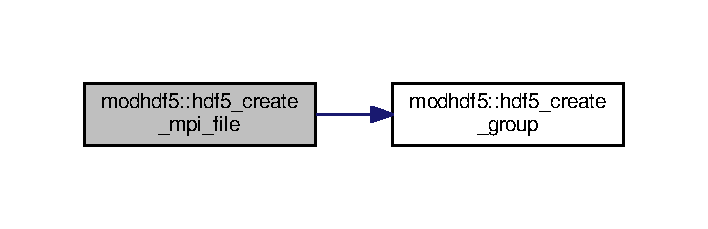
\includegraphics[width=340pt]{classmodhdf5_aba50f37e2c24ac3271cdfc8877ebdcd9_cgraph}
\end{center}
\end{figure}




Here is the caller graph for this function\-:\nopagebreak
\begin{figure}[H]
\begin{center}
\leavevmode
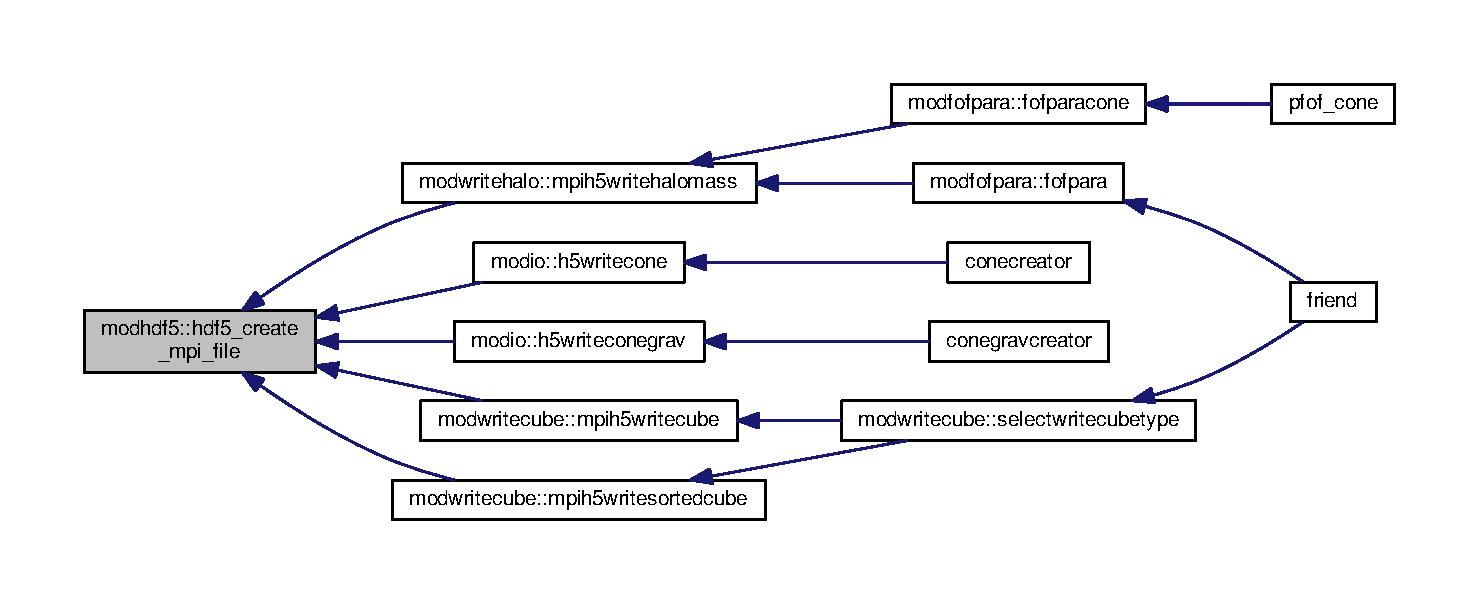
\includegraphics[width=350pt]{classmodhdf5_aba50f37e2c24ac3271cdfc8877ebdcd9_icgraph}
\end{center}
\end{figure}


\hypertarget{classmodhdf5_ace643e6a3e592dbe1be4d158888eb477}{\index{modhdf5@{modhdf5}!hdf5\-\_\-finalize@{hdf5\-\_\-finalize}}
\index{hdf5\-\_\-finalize@{hdf5\-\_\-finalize}!modhdf5@{modhdf5}}
\subsubsection[{hdf5\-\_\-finalize}]{\setlength{\rightskip}{0pt plus 5cm}subroutine, public modhdf5\-::hdf5\-\_\-finalize (
\begin{DoxyParamCaption}
{}
\end{DoxyParamCaption}
)}}\label{classmodhdf5_ace643e6a3e592dbe1be4d158888eb477}


Close the hdf5 interface. 



Definition at line 181 of file modhdf5.\-f90.



Here is the caller graph for this function\-:\nopagebreak
\begin{figure}[H]
\begin{center}
\leavevmode
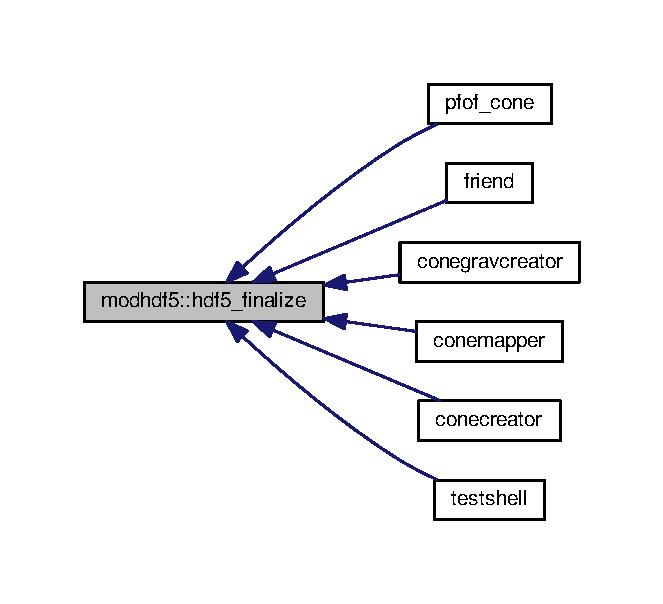
\includegraphics[width=318pt]{classmodhdf5_ace643e6a3e592dbe1be4d158888eb477_icgraph}
\end{center}
\end{figure}


\hypertarget{classmodhdf5_a78ec7a0bfdcd60f1ce1ecf0c88bb7cd9}{\index{modhdf5@{modhdf5}!hdf5\-\_\-init@{hdf5\-\_\-init}}
\index{hdf5\-\_\-init@{hdf5\-\_\-init}!modhdf5@{modhdf5}}
\subsubsection[{hdf5\-\_\-init}]{\setlength{\rightskip}{0pt plus 5cm}subroutine, public modhdf5\-::hdf5\-\_\-init (
\begin{DoxyParamCaption}
{}
\end{DoxyParamCaption}
)}}\label{classmodhdf5_a78ec7a0bfdcd60f1ce1ecf0c88bb7cd9}


Open the hdf5 interface. 



Definition at line 163 of file modhdf5.\-f90.



Here is the caller graph for this function\-:\nopagebreak
\begin{figure}[H]
\begin{center}
\leavevmode
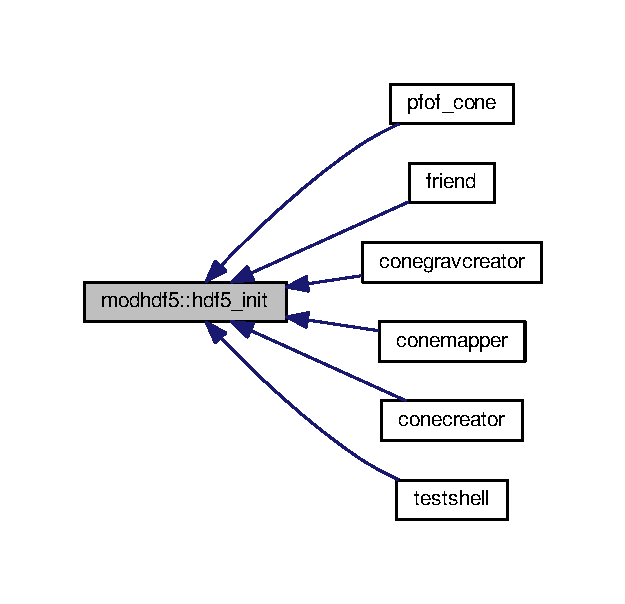
\includegraphics[width=300pt]{classmodhdf5_a78ec7a0bfdcd60f1ce1ecf0c88bb7cd9_icgraph}
\end{center}
\end{figure}


\hypertarget{classmodhdf5_a11539d06d180bff29d3c56ba198451d4}{\index{modhdf5@{modhdf5}!hdf5\-\_\-open\-\_\-file@{hdf5\-\_\-open\-\_\-file}}
\index{hdf5\-\_\-open\-\_\-file@{hdf5\-\_\-open\-\_\-file}!modhdf5@{modhdf5}}
\subsubsection[{hdf5\-\_\-open\-\_\-file}]{\setlength{\rightskip}{0pt plus 5cm}subroutine, public modhdf5\-::hdf5\-\_\-open\-\_\-file (
\begin{DoxyParamCaption}
\item[{character(len=400), intent(in)}]{filename, }
\item[{integer(kind=hid\-\_\-t), intent(out)}]{file\-\_\-id}
\end{DoxyParamCaption}
)}}\label{classmodhdf5_a11539d06d180bff29d3c56ba198451d4}


Open an existing hdf5 file. 


\begin{DoxyParams}[1]{Parameters}
\mbox{\tt in}  & {\em filename} & name of the file to open\\
\hline
\mbox{\tt out}  & {\em file\-\_\-id} & hdf5 id of the opened file \\
\hline
\end{DoxyParams}


Definition at line 203 of file modhdf5.\-f90.



Here is the caller graph for this function\-:\nopagebreak
\begin{figure}[H]
\begin{center}
\leavevmode
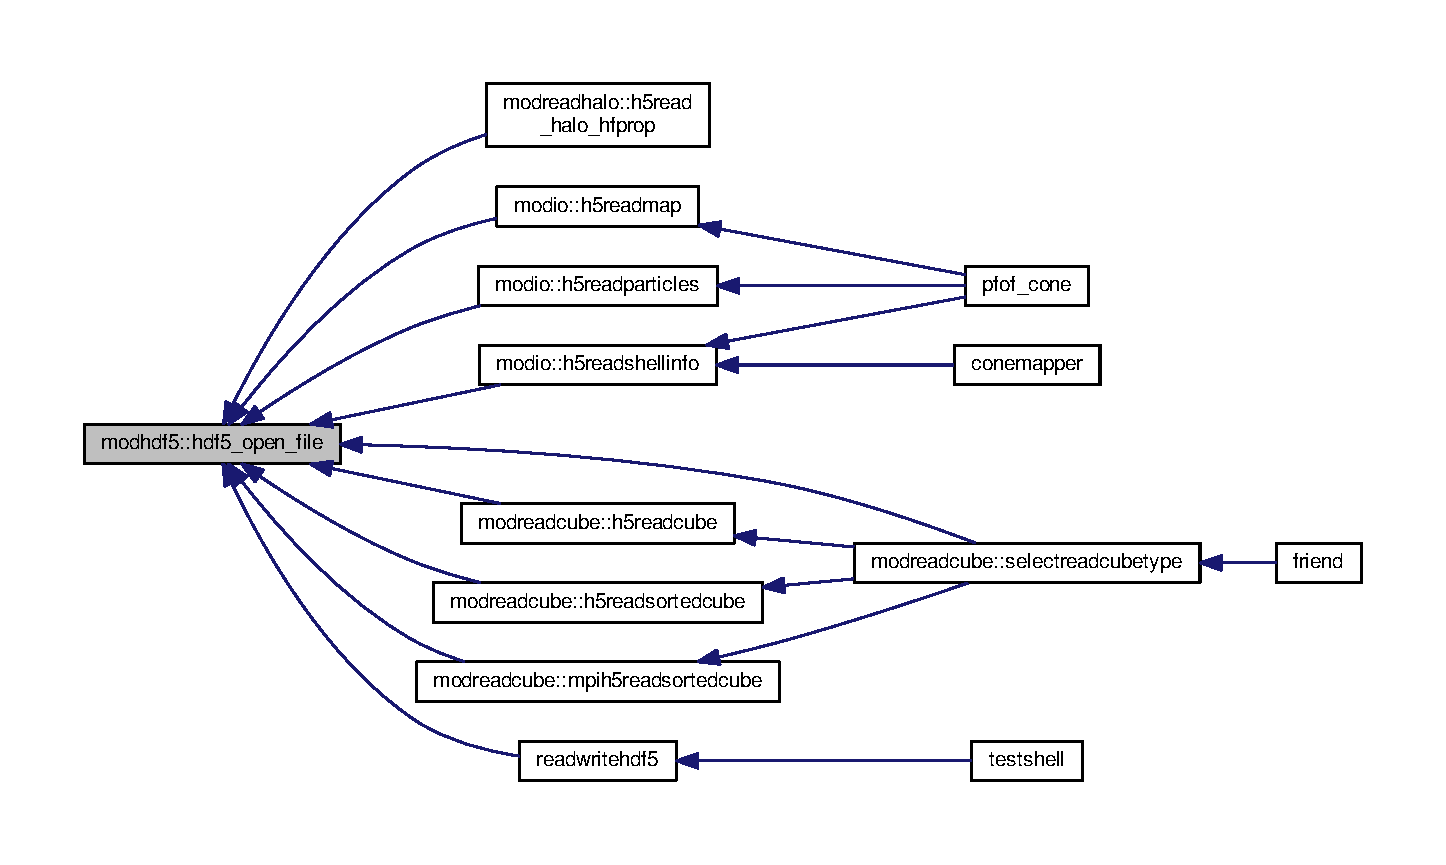
\includegraphics[width=350pt]{classmodhdf5_a11539d06d180bff29d3c56ba198451d4_icgraph}
\end{center}
\end{figure}


\hypertarget{classmodhdf5_ae547666d0167e2a78d6529e11c1faa92}{\index{modhdf5@{modhdf5}!hdf5\-\_\-open\-\_\-group@{hdf5\-\_\-open\-\_\-group}}
\index{hdf5\-\_\-open\-\_\-group@{hdf5\-\_\-open\-\_\-group}!modhdf5@{modhdf5}}
\subsubsection[{hdf5\-\_\-open\-\_\-group}]{\setlength{\rightskip}{0pt plus 5cm}subroutine, public modhdf5\-::hdf5\-\_\-open\-\_\-group (
\begin{DoxyParamCaption}
\item[{integer(hid\-\_\-t), intent(in)}]{id, }
\item[{character(len={\bf h5strlen}), intent(in)}]{name, }
\item[{integer(hid\-\_\-t), intent(out)}]{group\-\_\-id}
\end{DoxyParamCaption}
)}}\label{classmodhdf5_ae547666d0167e2a78d6529e11c1faa92}


Open an existing hdf5 group. 


\begin{DoxyParams}[1]{Parameters}
\mbox{\tt in}  & {\em id} & \char`\"{}parent\char`\"{} identifier\\
\hline
\mbox{\tt in}  & {\em name} & group name\\
\hline
\mbox{\tt out}  & {\em group\-\_\-id} & group identifier \\
\hline
\end{DoxyParams}


Definition at line 476 of file modhdf5.\-f90.



Here is the caller graph for this function\-:\nopagebreak
\begin{figure}[H]
\begin{center}
\leavevmode
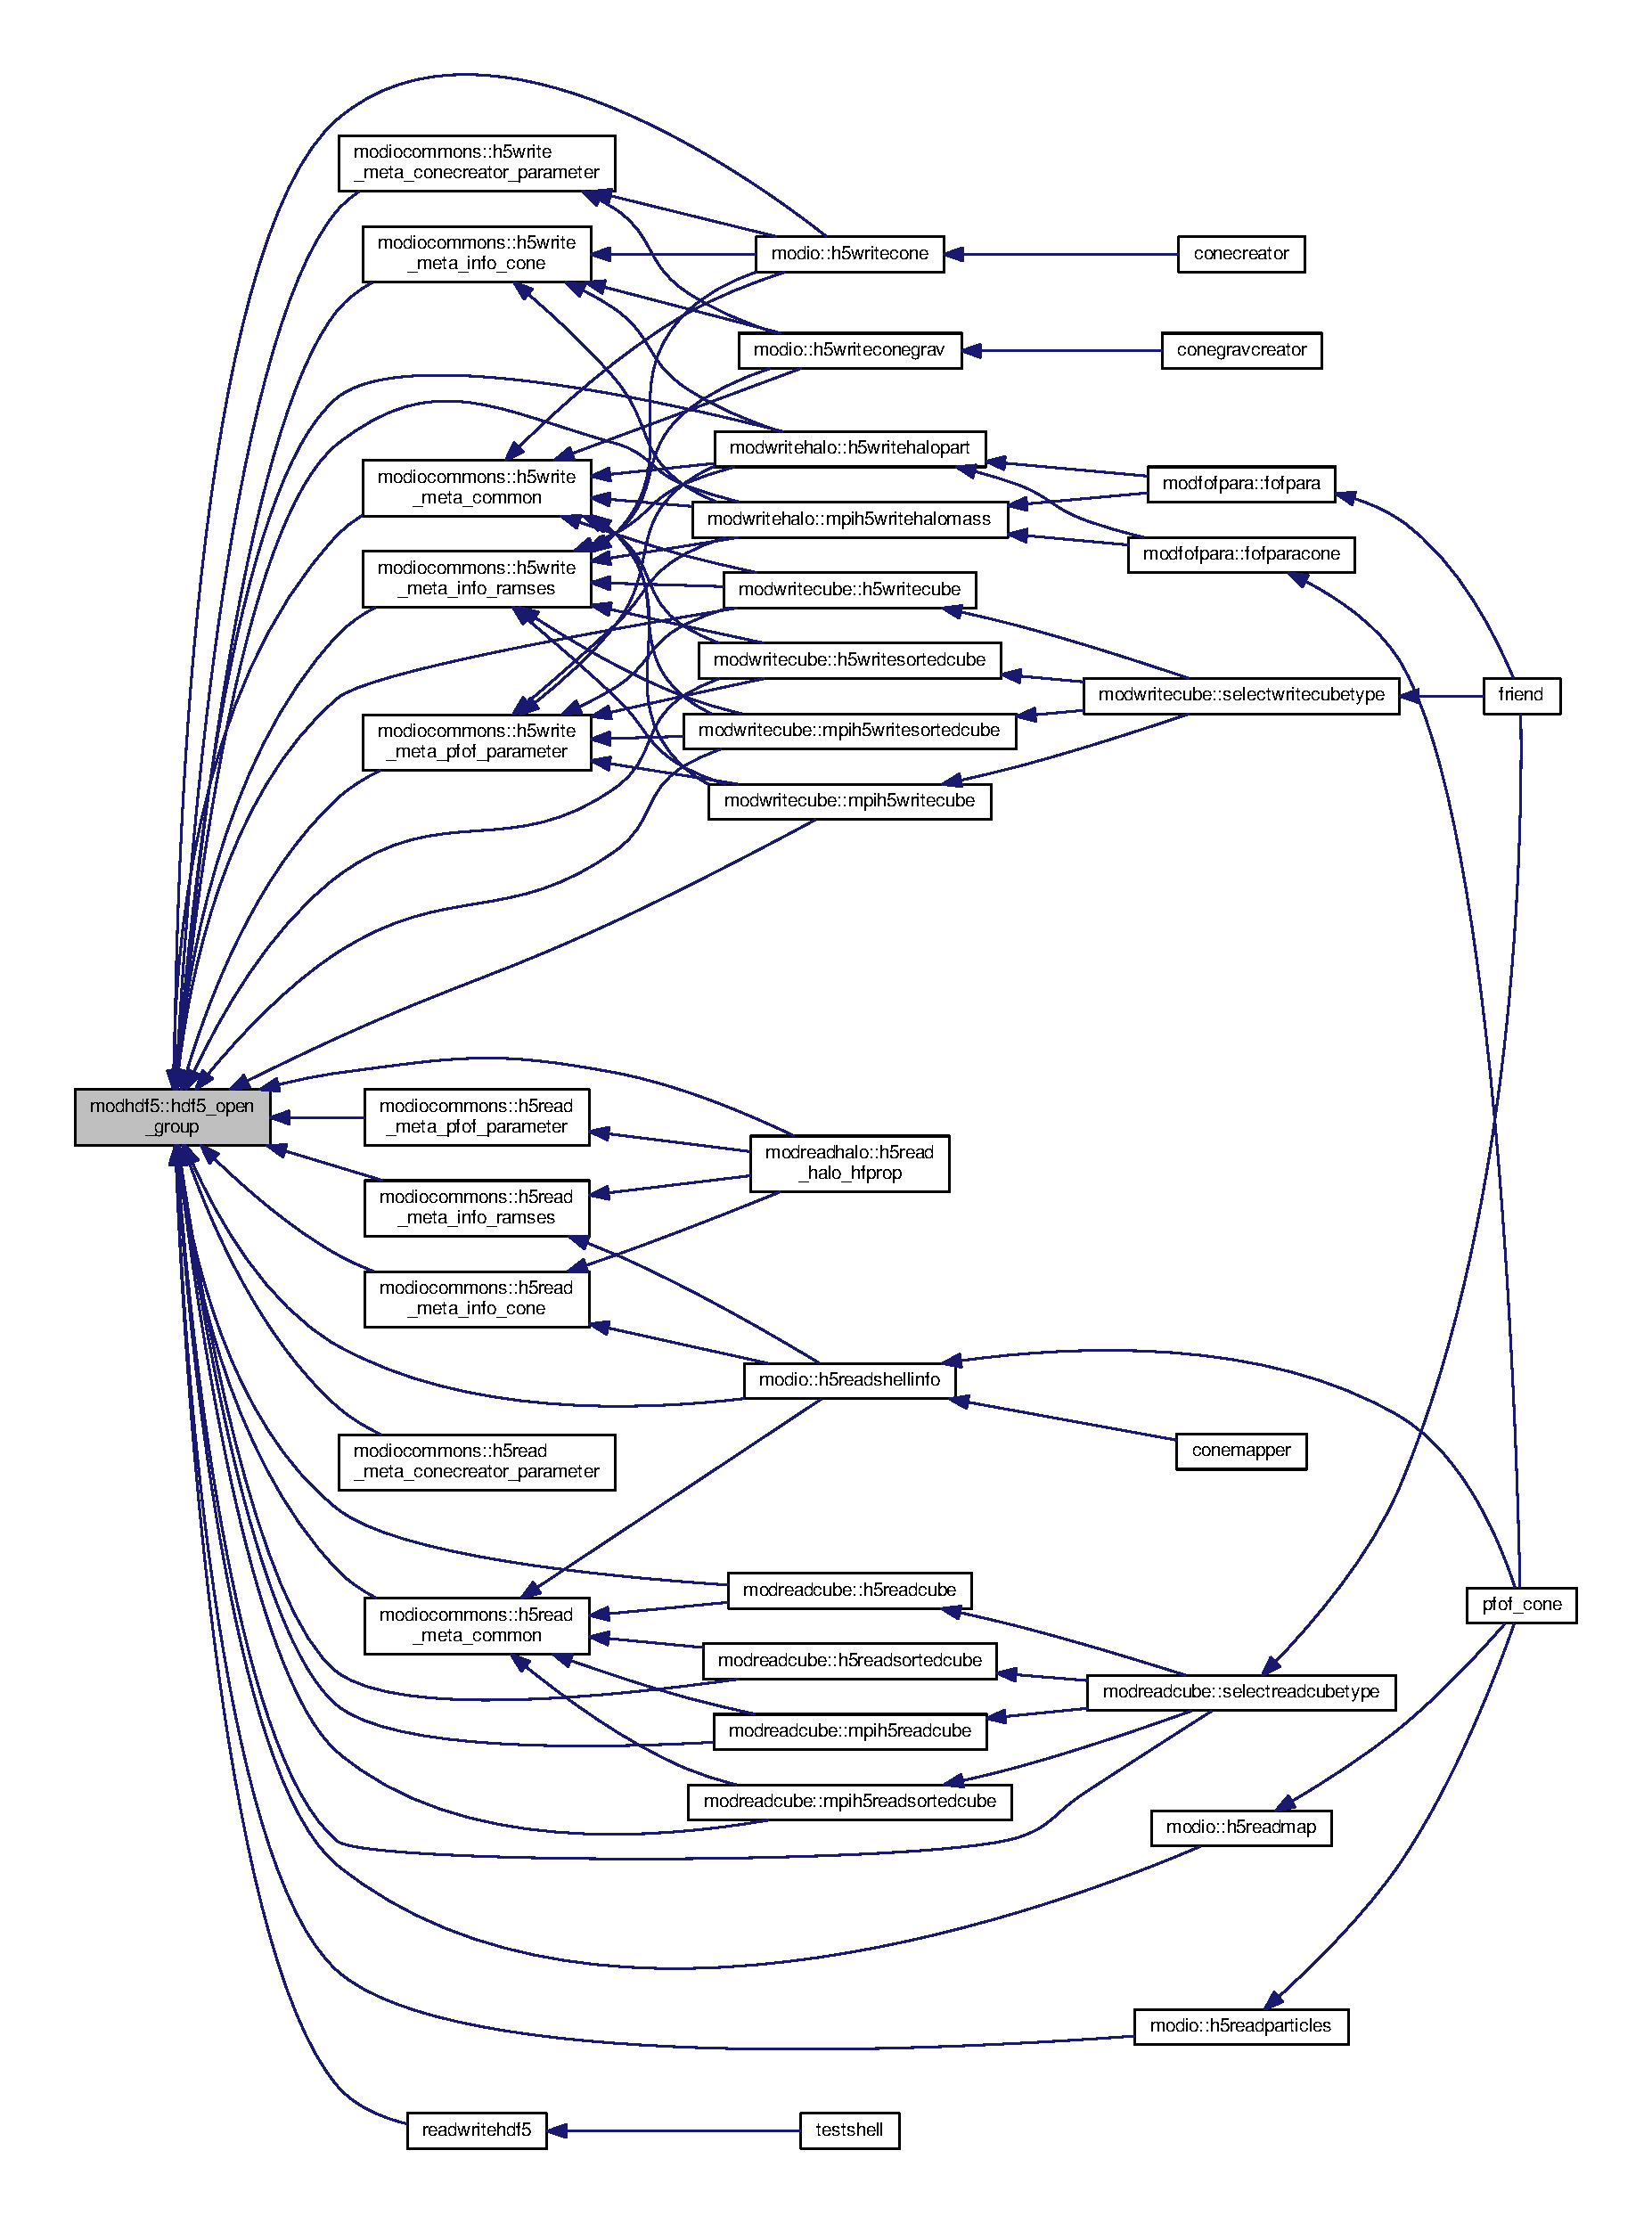
\includegraphics[width=350pt]{classmodhdf5_ae547666d0167e2a78d6529e11c1faa92_icgraph}
\end{center}
\end{figure}


\hypertarget{classmodhdf5_a9f6976ee158485f6b203635df23156e3}{\index{modhdf5@{modhdf5}!hdf5\-\_\-open\-\_\-mpi\-\_\-file@{hdf5\-\_\-open\-\_\-mpi\-\_\-file}}
\index{hdf5\-\_\-open\-\_\-mpi\-\_\-file@{hdf5\-\_\-open\-\_\-mpi\-\_\-file}!modhdf5@{modhdf5}}
\subsubsection[{hdf5\-\_\-open\-\_\-mpi\-\_\-file}]{\setlength{\rightskip}{0pt plus 5cm}subroutine, public modhdf5\-::hdf5\-\_\-open\-\_\-mpi\-\_\-file (
\begin{DoxyParamCaption}
\item[{character(len=400), intent(in)}]{filename, }
\item[{integer(kind=4), intent(in)}]{comm, }
\item[{integer(kind=hid\-\_\-t), intent(out)}]{file\-\_\-id}
\end{DoxyParamCaption}
)}}\label{classmodhdf5_a9f6976ee158485f6b203635df23156e3}


Open an existing 'parallel' hdf5 file shared by the communicator comm. 


\begin{DoxyParams}[1]{Parameters}
\mbox{\tt in}  & {\em filename} & name of the parallel file to open\\
\hline
\mbox{\tt in}  & {\em comm} & M\-P\-I communicator used for the file access\\
\hline
\mbox{\tt out}  & {\em file\-\_\-id} & hdf5 id of the opened file \\
\hline
\end{DoxyParams}


Definition at line 229 of file modhdf5.\-f90.



Here is the caller graph for this function\-:\nopagebreak
\begin{figure}[H]
\begin{center}
\leavevmode
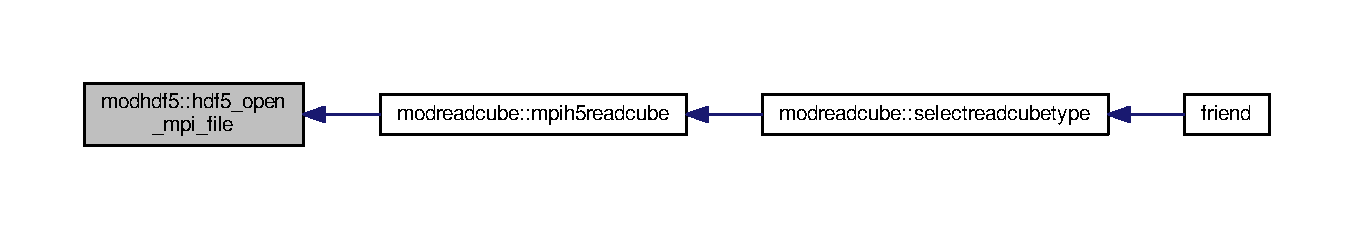
\includegraphics[width=350pt]{classmodhdf5_a9f6976ee158485f6b203635df23156e3_icgraph}
\end{center}
\end{figure}


\hypertarget{classmodhdf5_a2da336bc6d0ebbf1e6d582469b741a63}{\index{modhdf5@{modhdf5}!hdf5\-\_\-read\-\_\-char\-\_\-attr@{hdf5\-\_\-read\-\_\-char\-\_\-attr}}
\index{hdf5\-\_\-read\-\_\-char\-\_\-attr@{hdf5\-\_\-read\-\_\-char\-\_\-attr}!modhdf5@{modhdf5}}
\subsubsection[{hdf5\-\_\-read\-\_\-char\-\_\-attr}]{\setlength{\rightskip}{0pt plus 5cm}subroutine modhdf5\-::hdf5\-\_\-read\-\_\-char\-\_\-attr (
\begin{DoxyParamCaption}
\item[{integer(kind=hid\-\_\-t), intent(in)}]{id, }
\item[{character(len={\bf h5strlen}), intent(in)}]{name, }
\item[{integer(kind=4), intent(in)}]{n1, }
\item[{character(len=n1), intent(inout)}]{attr}
\end{DoxyParamCaption}
)\hspace{0.3cm}{\ttfamily [private]}}}\label{classmodhdf5_a2da336bc6d0ebbf1e6d582469b741a63}


Read string attribute in a hdf5 file. 


\begin{DoxyParams}[1]{Parameters}
\mbox{\tt in}  & {\em id} & id of the file/group where the attribute will be read\\
\hline
\mbox{\tt in}  & {\em name} & name of the attribute\\
\hline
\mbox{\tt in}  & {\em n1} & dimension of the attribute string\\
\hline
\mbox{\tt in,out}  & {\em attr} & attribute value \\
\hline
\end{DoxyParams}


Definition at line 3257 of file modhdf5.\-f90.

\hypertarget{classmodhdf5_afda2e44922def0d140ce850c12ef2f48}{\index{modhdf5@{modhdf5}!hdf5\-\_\-read\-\_\-int4\-\_\-1d@{hdf5\-\_\-read\-\_\-int4\-\_\-1d}}
\index{hdf5\-\_\-read\-\_\-int4\-\_\-1d@{hdf5\-\_\-read\-\_\-int4\-\_\-1d}!modhdf5@{modhdf5}}
\subsubsection[{hdf5\-\_\-read\-\_\-int4\-\_\-1d}]{\setlength{\rightskip}{0pt plus 5cm}subroutine modhdf5\-::hdf5\-\_\-read\-\_\-int4\-\_\-1d (
\begin{DoxyParamCaption}
\item[{integer(hid\-\_\-t), intent(in)}]{id, }
\item[{character(len={\bf h5strlen}), intent(in)}]{name, }
\item[{integer(kind=4), intent(in)}]{n1, }
\item[{integer(kind=4), dimension(n1), intent(inout), target}]{data}
\end{DoxyParamCaption}
)\hspace{0.3cm}{\ttfamily [private]}}}\label{classmodhdf5_afda2e44922def0d140ce850c12ef2f48}


Read a 1-\/\-D integer(kind=4) array from a serial file. 


\begin{DoxyParams}[1]{Parameters}
\mbox{\tt in}  & {\em id} & id of the file/group where the dataset will be read\\
\hline
\mbox{\tt in}  & {\em name} & name of the dataset\\
\hline
\mbox{\tt in}  & {\em n1} & dimension of the array to read\\
\hline
\mbox{\tt in,out}  & {\em data} & array \\
\hline
\end{DoxyParams}


Definition at line 1731 of file modhdf5.\-f90.

\hypertarget{classmodhdf5_a29f383042b1dc2b1fc1155af48fc98a3}{\index{modhdf5@{modhdf5}!hdf5\-\_\-read\-\_\-int4\-\_\-2d@{hdf5\-\_\-read\-\_\-int4\-\_\-2d}}
\index{hdf5\-\_\-read\-\_\-int4\-\_\-2d@{hdf5\-\_\-read\-\_\-int4\-\_\-2d}!modhdf5@{modhdf5}}
\subsubsection[{hdf5\-\_\-read\-\_\-int4\-\_\-2d}]{\setlength{\rightskip}{0pt plus 5cm}subroutine modhdf5\-::hdf5\-\_\-read\-\_\-int4\-\_\-2d (
\begin{DoxyParamCaption}
\item[{integer(hid\-\_\-t), intent(in)}]{id, }
\item[{character(len={\bf h5strlen}), intent(in)}]{name, }
\item[{integer(kind=4), intent(in)}]{n1, }
\item[{integer(kind=4), intent(in)}]{n2, }
\item[{integer(kind=4), dimension(n1,n2), intent(inout), target}]{data}
\end{DoxyParamCaption}
)\hspace{0.3cm}{\ttfamily [private]}}}\label{classmodhdf5_a29f383042b1dc2b1fc1155af48fc98a3}


Read a 2-\/\-D integer(kind=4) array from a serial file. 


\begin{DoxyParams}[1]{Parameters}
\mbox{\tt in}  & {\em id} & id of the file/group where the dataset will be read\\
\hline
\mbox{\tt in}  & {\em name} & name of the dataset\\
\hline
\mbox{\tt in}  & {\em n1} & first dimension of the array to read\\
\hline
\mbox{\tt in}  & {\em n2} & second dimension of the array to read\\
\hline
\mbox{\tt in,out}  & {\em data} & array \\
\hline
\end{DoxyParams}


Definition at line 1838 of file modhdf5.\-f90.

\hypertarget{classmodhdf5_a10a4b5212d77e52dba2616ba3abb7df1}{\index{modhdf5@{modhdf5}!hdf5\-\_\-read\-\_\-int4\-\_\-attr0d@{hdf5\-\_\-read\-\_\-int4\-\_\-attr0d}}
\index{hdf5\-\_\-read\-\_\-int4\-\_\-attr0d@{hdf5\-\_\-read\-\_\-int4\-\_\-attr0d}!modhdf5@{modhdf5}}
\subsubsection[{hdf5\-\_\-read\-\_\-int4\-\_\-attr0d}]{\setlength{\rightskip}{0pt plus 5cm}subroutine modhdf5\-::hdf5\-\_\-read\-\_\-int4\-\_\-attr0d (
\begin{DoxyParamCaption}
\item[{integer(kind=hid\-\_\-t), intent(in)}]{id, }
\item[{character(len={\bf h5strlen}), intent(in)}]{name, }
\item[{integer(kind=4), intent(inout)}]{attr}
\end{DoxyParamCaption}
)\hspace{0.3cm}{\ttfamily [private]}}}\label{classmodhdf5_a10a4b5212d77e52dba2616ba3abb7df1}


Read an integer4 attribute in a hdf5 file. 


\begin{DoxyParams}[1]{Parameters}
\mbox{\tt in}  & {\em id} & id of the file/group where the attribute will be read\\
\hline
\mbox{\tt in}  & {\em name} & name of the attribute\\
\hline
\mbox{\tt in,out}  & {\em attr} & attribute value \\
\hline
\end{DoxyParams}


Definition at line 3025 of file modhdf5.\-f90.

\hypertarget{classmodhdf5_a2ff1b28dd896cc37583e97a52348039f}{\index{modhdf5@{modhdf5}!hdf5\-\_\-read\-\_\-int4\-\_\-attr1d@{hdf5\-\_\-read\-\_\-int4\-\_\-attr1d}}
\index{hdf5\-\_\-read\-\_\-int4\-\_\-attr1d@{hdf5\-\_\-read\-\_\-int4\-\_\-attr1d}!modhdf5@{modhdf5}}
\subsubsection[{hdf5\-\_\-read\-\_\-int4\-\_\-attr1d}]{\setlength{\rightskip}{0pt plus 5cm}subroutine modhdf5\-::hdf5\-\_\-read\-\_\-int4\-\_\-attr1d (
\begin{DoxyParamCaption}
\item[{integer(kind=hid\-\_\-t), intent(in)}]{id, }
\item[{character(len={\bf h5strlen}), intent(in)}]{name, }
\item[{integer(kind=4), intent(in)}]{n1, }
\item[{integer(kind=4), dimension(n1), intent(inout)}]{attr}
\end{DoxyParamCaption}
)\hspace{0.3cm}{\ttfamily [private]}}}\label{classmodhdf5_a2ff1b28dd896cc37583e97a52348039f}


Read a 1-\/\-D integer4 attribute in a hdf5 file. 


\begin{DoxyParams}[1]{Parameters}
\mbox{\tt in}  & {\em id} & id of the file/group where the attribute will be read\\
\hline
\mbox{\tt in}  & {\em name} & name of the attribute\\
\hline
\mbox{\tt in}  & {\em n1} & dimension of the attribute array\\
\hline
\mbox{\tt in,out}  & {\em attr} & attribute value \\
\hline
\end{DoxyParams}


Definition at line 3053 of file modhdf5.\-f90.

\hypertarget{classmodhdf5_a4ca8f47995bf9df5b6c892781c87dd95}{\index{modhdf5@{modhdf5}!hdf5\-\_\-read\-\_\-int4\-\_\-attr2d@{hdf5\-\_\-read\-\_\-int4\-\_\-attr2d}}
\index{hdf5\-\_\-read\-\_\-int4\-\_\-attr2d@{hdf5\-\_\-read\-\_\-int4\-\_\-attr2d}!modhdf5@{modhdf5}}
\subsubsection[{hdf5\-\_\-read\-\_\-int4\-\_\-attr2d}]{\setlength{\rightskip}{0pt plus 5cm}subroutine modhdf5\-::hdf5\-\_\-read\-\_\-int4\-\_\-attr2d (
\begin{DoxyParamCaption}
\item[{integer(kind=hid\-\_\-t), intent(in)}]{id, }
\item[{character(len={\bf h5strlen}), intent(in)}]{name, }
\item[{integer(kind=4), intent(in)}]{n1, }
\item[{integer(kind=4), intent(in)}]{n2, }
\item[{integer(kind=4), dimension(n1,n2), intent(inout)}]{attr}
\end{DoxyParamCaption}
)\hspace{0.3cm}{\ttfamily [private]}}}\label{classmodhdf5_a4ca8f47995bf9df5b6c892781c87dd95}


Read a 2-\/\-D integer4 attribute in a hdf5 file. 


\begin{DoxyParams}[1]{Parameters}
\mbox{\tt in}  & {\em id} & id of the file/group where the attribute will be read\\
\hline
\mbox{\tt in}  & {\em name} & name of the attribute\\
\hline
\mbox{\tt in}  & {\em n1} & first dimension of the attribute array\\
\hline
\mbox{\tt in}  & {\em n2} & second dimension of the attribute array\\
\hline
\mbox{\tt in,out}  & {\em attr} & attribute value \\
\hline
\end{DoxyParams}


Definition at line 3078 of file modhdf5.\-f90.

\hypertarget{classmodhdf5_ac60e719f8d357b8ffab4f183a7ca4603}{\index{modhdf5@{modhdf5}!hdf5\-\_\-read\-\_\-int8\-\_\-0d@{hdf5\-\_\-read\-\_\-int8\-\_\-0d}}
\index{hdf5\-\_\-read\-\_\-int8\-\_\-0d@{hdf5\-\_\-read\-\_\-int8\-\_\-0d}!modhdf5@{modhdf5}}
\subsubsection[{hdf5\-\_\-read\-\_\-int8\-\_\-0d}]{\setlength{\rightskip}{0pt plus 5cm}subroutine modhdf5\-::hdf5\-\_\-read\-\_\-int8\-\_\-0d (
\begin{DoxyParamCaption}
\item[{integer(hid\-\_\-t), intent(in)}]{id, }
\item[{character(len={\bf h5strlen}), intent(in)}]{name, }
\item[{integer(kind=8), intent(inout), target}]{data}
\end{DoxyParamCaption}
)\hspace{0.3cm}{\ttfamily [private]}}}\label{classmodhdf5_ac60e719f8d357b8ffab4f183a7ca4603}


Read a 1-\/\-D integer(kind=8) scalar from a serial file. 


\begin{DoxyParams}[1]{Parameters}
\mbox{\tt in}  & {\em id} & id of the file/group where the dataset will be read\\
\hline
\mbox{\tt in}  & {\em name} & name of the dataset\\
\hline
\mbox{\tt in,out}  & {\em data} & array \\
\hline
\end{DoxyParams}


Definition at line 1777 of file modhdf5.\-f90.

\hypertarget{classmodhdf5_a640df6ccea7f28d6ed6b578d8018d7d7}{\index{modhdf5@{modhdf5}!hdf5\-\_\-read\-\_\-int8\-\_\-1d@{hdf5\-\_\-read\-\_\-int8\-\_\-1d}}
\index{hdf5\-\_\-read\-\_\-int8\-\_\-1d@{hdf5\-\_\-read\-\_\-int8\-\_\-1d}!modhdf5@{modhdf5}}
\subsubsection[{hdf5\-\_\-read\-\_\-int8\-\_\-1d}]{\setlength{\rightskip}{0pt plus 5cm}subroutine modhdf5\-::hdf5\-\_\-read\-\_\-int8\-\_\-1d (
\begin{DoxyParamCaption}
\item[{integer(hid\-\_\-t), intent(in)}]{id, }
\item[{character(len={\bf h5strlen}), intent(in)}]{name, }
\item[{integer(kind=4), intent(in)}]{n1, }
\item[{integer(kind=8), dimension(n1), intent(inout), target}]{data}
\end{DoxyParamCaption}
)\hspace{0.3cm}{\ttfamily [private]}}}\label{classmodhdf5_a640df6ccea7f28d6ed6b578d8018d7d7}


Read a 1-\/\-D integer(kind=8) array from a serial file. 


\begin{DoxyParams}[1]{Parameters}
\mbox{\tt in}  & {\em id} & id of the file/group where the dataset will be read\\
\hline
\mbox{\tt in}  & {\em name} & name of the dataset\\
\hline
\mbox{\tt in}  & {\em n1} & dimension of the array to read\\
\hline
\mbox{\tt in,out}  & {\em data} & array \\
\hline
\end{DoxyParams}


Definition at line 1807 of file modhdf5.\-f90.

\hypertarget{classmodhdf5_a4ac00fa4fbae4c8a8f936ee48292e114}{\index{modhdf5@{modhdf5}!hdf5\-\_\-read\-\_\-int8\-\_\-2d@{hdf5\-\_\-read\-\_\-int8\-\_\-2d}}
\index{hdf5\-\_\-read\-\_\-int8\-\_\-2d@{hdf5\-\_\-read\-\_\-int8\-\_\-2d}!modhdf5@{modhdf5}}
\subsubsection[{hdf5\-\_\-read\-\_\-int8\-\_\-2d}]{\setlength{\rightskip}{0pt plus 5cm}subroutine modhdf5\-::hdf5\-\_\-read\-\_\-int8\-\_\-2d (
\begin{DoxyParamCaption}
\item[{integer(hid\-\_\-t), intent(in)}]{id, }
\item[{character(len={\bf h5strlen}), intent(in)}]{name, }
\item[{integer(kind=4), intent(in)}]{n1, }
\item[{integer(kind=4), intent(in)}]{n2, }
\item[{integer(kind=8), dimension(n1,n2), intent(inout), target}]{data}
\end{DoxyParamCaption}
)\hspace{0.3cm}{\ttfamily [private]}}}\label{classmodhdf5_a4ac00fa4fbae4c8a8f936ee48292e114}


Read a 2-\/\-D integer(kind=8) array from a serial file. 


\begin{DoxyParams}[1]{Parameters}
\mbox{\tt in}  & {\em id} & id of the file/group where the dataset will be read\\
\hline
\mbox{\tt in}  & {\em name} & name of the dataset\\
\hline
\mbox{\tt in}  & {\em n1} & first dimension of the array to read\\
\hline
\mbox{\tt in}  & {\em n2} & second dimension of the array to read\\
\hline
\mbox{\tt in,out}  & {\em data} & array \\
\hline
\end{DoxyParams}


Definition at line 1870 of file modhdf5.\-f90.

\hypertarget{classmodhdf5_a18b987f7a44198ccc7dd893cbdc322fc}{\index{modhdf5@{modhdf5}!hdf5\-\_\-read\-\_\-mpi\-\_\-int4\-\_\-1d@{hdf5\-\_\-read\-\_\-mpi\-\_\-int4\-\_\-1d}}
\index{hdf5\-\_\-read\-\_\-mpi\-\_\-int4\-\_\-1d@{hdf5\-\_\-read\-\_\-mpi\-\_\-int4\-\_\-1d}!modhdf5@{modhdf5}}
\subsubsection[{hdf5\-\_\-read\-\_\-mpi\-\_\-int4\-\_\-1d}]{\setlength{\rightskip}{0pt plus 5cm}subroutine modhdf5\-::hdf5\-\_\-read\-\_\-mpi\-\_\-int4\-\_\-1d (
\begin{DoxyParamCaption}
\item[{integer(hid\-\_\-t), intent(in)}]{id, }
\item[{character(len={\bf h5strlen}), intent(in)}]{name, }
\item[{integer(kind=4), intent(in)}]{n1, }
\item[{integer(kind=4), dimension(n1), intent(inout), target}]{data, }
\item[{integer(kind=4), intent(in)}]{comm}
\end{DoxyParamCaption}
)\hspace{0.3cm}{\ttfamily [private]}}}\label{classmodhdf5_a18b987f7a44198ccc7dd893cbdc322fc}


Read a 1-\/\-D integer4 array from a parallel file The array is distributed along the 2nd dimension. 


\begin{DoxyParams}[1]{Parameters}
\mbox{\tt in}  & {\em id} & id of the file/group where the dataset will be read\\
\hline
\mbox{\tt in}  & {\em name} & name of the dataset\\
\hline
\mbox{\tt in}  & {\em n1} & dimension of the local array to read\\
\hline
\mbox{\tt in,out}  & {\em data} & array\\
\hline
\mbox{\tt in}  & {\em comm} & M\-P\-I communicator used \\
\hline
\end{DoxyParams}


Definition at line 2034 of file modhdf5.\-f90.

\hypertarget{classmodhdf5_ac96ae5057bcd6745840c716a232d4b66}{\index{modhdf5@{modhdf5}!hdf5\-\_\-read\-\_\-mpi\-\_\-int4\-\_\-2d@{hdf5\-\_\-read\-\_\-mpi\-\_\-int4\-\_\-2d}}
\index{hdf5\-\_\-read\-\_\-mpi\-\_\-int4\-\_\-2d@{hdf5\-\_\-read\-\_\-mpi\-\_\-int4\-\_\-2d}!modhdf5@{modhdf5}}
\subsubsection[{hdf5\-\_\-read\-\_\-mpi\-\_\-int4\-\_\-2d}]{\setlength{\rightskip}{0pt plus 5cm}subroutine modhdf5\-::hdf5\-\_\-read\-\_\-mpi\-\_\-int4\-\_\-2d (
\begin{DoxyParamCaption}
\item[{integer(hid\-\_\-t), intent(in)}]{id, }
\item[{character(len={\bf h5strlen}), intent(in)}]{name, }
\item[{integer(kind=4), intent(in)}]{n1, }
\item[{integer(kind=4), intent(in)}]{n2, }
\item[{integer(kind=4), dimension(n1,n2), intent(inout), target}]{data, }
\item[{integer(kind=4), intent(in)}]{comm}
\end{DoxyParamCaption}
)\hspace{0.3cm}{\ttfamily [private]}}}\label{classmodhdf5_ac96ae5057bcd6745840c716a232d4b66}


Read a 2-\/\-D integer4 array from a parallel file The array is distributed along the 2nd dimension. 


\begin{DoxyParams}[1]{Parameters}
\mbox{\tt in}  & {\em id} & id of the file/group where the dataset will be read\\
\hline
\mbox{\tt in}  & {\em name} & name of the dataset\\
\hline
\mbox{\tt in}  & {\em n1} & first dimension of the local array to read\\
\hline
\mbox{\tt in}  & {\em n2} & second dimension of the local array to read\\
\hline
\mbox{\tt in,out}  & {\em data} & array\\
\hline
\mbox{\tt in}  & {\em comm} & M\-P\-I communicator used \\
\hline
\end{DoxyParams}


Definition at line 2110 of file modhdf5.\-f90.

\hypertarget{classmodhdf5_a2847f70176f88d95e8e6e1bec3a2539e}{\index{modhdf5@{modhdf5}!hdf5\-\_\-read\-\_\-mpi\-\_\-int8\-\_\-1d@{hdf5\-\_\-read\-\_\-mpi\-\_\-int8\-\_\-1d}}
\index{hdf5\-\_\-read\-\_\-mpi\-\_\-int8\-\_\-1d@{hdf5\-\_\-read\-\_\-mpi\-\_\-int8\-\_\-1d}!modhdf5@{modhdf5}}
\subsubsection[{hdf5\-\_\-read\-\_\-mpi\-\_\-int8\-\_\-1d}]{\setlength{\rightskip}{0pt plus 5cm}subroutine modhdf5\-::hdf5\-\_\-read\-\_\-mpi\-\_\-int8\-\_\-1d (
\begin{DoxyParamCaption}
\item[{integer(hid\-\_\-t), intent(in)}]{id, }
\item[{character(len={\bf h5strlen}), intent(in)}]{name, }
\item[{integer(kind=4), intent(in)}]{n1, }
\item[{integer(kind=8), dimension(n1), intent(inout), target}]{data, }
\item[{integer(kind=4), intent(in)}]{comm}
\end{DoxyParamCaption}
)\hspace{0.3cm}{\ttfamily [private]}}}\label{classmodhdf5_a2847f70176f88d95e8e6e1bec3a2539e}


Read a 1-\/\-D integer8 array from a parallel file The array is distributed along the 2nd dimension. 


\begin{DoxyParams}[1]{Parameters}
\mbox{\tt in}  & {\em id} & id of the file/group where the dataset will be read\\
\hline
\mbox{\tt in}  & {\em name} & name of the dataset\\
\hline
\mbox{\tt in}  & {\em n1} & dimension of the local array to read\\
\hline
\mbox{\tt in,out}  & {\em data} & array\\
\hline
\mbox{\tt in}  & {\em comm} & M\-P\-I communicator used \\
\hline
\end{DoxyParams}


Definition at line 2190 of file modhdf5.\-f90.

\hypertarget{classmodhdf5_a41bc63b78ce861c9898ef45642514a9d}{\index{modhdf5@{modhdf5}!hdf5\-\_\-read\-\_\-mpi\-\_\-int8\-\_\-2d@{hdf5\-\_\-read\-\_\-mpi\-\_\-int8\-\_\-2d}}
\index{hdf5\-\_\-read\-\_\-mpi\-\_\-int8\-\_\-2d@{hdf5\-\_\-read\-\_\-mpi\-\_\-int8\-\_\-2d}!modhdf5@{modhdf5}}
\subsubsection[{hdf5\-\_\-read\-\_\-mpi\-\_\-int8\-\_\-2d}]{\setlength{\rightskip}{0pt plus 5cm}subroutine modhdf5\-::hdf5\-\_\-read\-\_\-mpi\-\_\-int8\-\_\-2d (
\begin{DoxyParamCaption}
\item[{integer(hid\-\_\-t), intent(in)}]{id, }
\item[{character(len={\bf h5strlen}), intent(in)}]{name, }
\item[{integer(kind=4), intent(in)}]{n1, }
\item[{integer(kind=4), intent(in)}]{n2, }
\item[{integer(kind=8), dimension(n1,n2), intent(inout), target}]{data, }
\item[{integer(kind=4), intent(in)}]{comm}
\end{DoxyParamCaption}
)\hspace{0.3cm}{\ttfamily [private]}}}\label{classmodhdf5_a41bc63b78ce861c9898ef45642514a9d}


Read a 2-\/\-D integer8 array from a parallel file The array is distributed along the 2nd dimension. 


\begin{DoxyParams}[1]{Parameters}
\mbox{\tt in}  & {\em id} & id of the file/group where the dataset will be read\\
\hline
\mbox{\tt in}  & {\em name} & name of the dataset\\
\hline
\mbox{\tt in}  & {\em n1} & first dimension of the local array to read\\
\hline
\mbox{\tt in}  & {\em n2} & second dimension of the local array to read\\
\hline
\mbox{\tt in,out}  & {\em data} & array\\
\hline
\mbox{\tt in}  & {\em comm} & M\-P\-I communicator used \\
\hline
\end{DoxyParams}


Definition at line 2267 of file modhdf5.\-f90.

\hypertarget{classmodhdf5_a7c2f69141e8a85768536e7c8f79f6348}{\index{modhdf5@{modhdf5}!hdf5\-\_\-read\-\_\-mpi\-\_\-real4\-\_\-1d@{hdf5\-\_\-read\-\_\-mpi\-\_\-real4\-\_\-1d}}
\index{hdf5\-\_\-read\-\_\-mpi\-\_\-real4\-\_\-1d@{hdf5\-\_\-read\-\_\-mpi\-\_\-real4\-\_\-1d}!modhdf5@{modhdf5}}
\subsubsection[{hdf5\-\_\-read\-\_\-mpi\-\_\-real4\-\_\-1d}]{\setlength{\rightskip}{0pt plus 5cm}subroutine modhdf5\-::hdf5\-\_\-read\-\_\-mpi\-\_\-real4\-\_\-1d (
\begin{DoxyParamCaption}
\item[{integer(hid\-\_\-t), intent(in)}]{id, }
\item[{character(len={\bf h5strlen}), intent(in)}]{name, }
\item[{integer(kind=4), intent(in)}]{n1, }
\item[{real(kind=4), dimension(n1), intent(inout), target}]{data, }
\item[{integer(kind=4), intent(in)}]{comm}
\end{DoxyParamCaption}
)\hspace{0.3cm}{\ttfamily [private]}}}\label{classmodhdf5_a7c2f69141e8a85768536e7c8f79f6348}


Read a 1-\/\-D real4 array from a parallel file The array is distributed along the 2nd dimension. 


\begin{DoxyParams}[1]{Parameters}
\mbox{\tt in}  & {\em id} & id of the file/group where the dataset will be read\\
\hline
\mbox{\tt in}  & {\em name} & name of the dataset\\
\hline
\mbox{\tt in}  & {\em n1} & dimension of the local array to read\\
\hline
\mbox{\tt in,out}  & {\em data} & array\\
\hline
\mbox{\tt in}  & {\em comm} & M\-P\-I communicator used \\
\hline
\end{DoxyParams}


Definition at line 2347 of file modhdf5.\-f90.

\hypertarget{classmodhdf5_a406b07a6320d4dd08a12ca4b8d6b9e9d}{\index{modhdf5@{modhdf5}!hdf5\-\_\-read\-\_\-mpi\-\_\-real4\-\_\-2d@{hdf5\-\_\-read\-\_\-mpi\-\_\-real4\-\_\-2d}}
\index{hdf5\-\_\-read\-\_\-mpi\-\_\-real4\-\_\-2d@{hdf5\-\_\-read\-\_\-mpi\-\_\-real4\-\_\-2d}!modhdf5@{modhdf5}}
\subsubsection[{hdf5\-\_\-read\-\_\-mpi\-\_\-real4\-\_\-2d}]{\setlength{\rightskip}{0pt plus 5cm}subroutine modhdf5\-::hdf5\-\_\-read\-\_\-mpi\-\_\-real4\-\_\-2d (
\begin{DoxyParamCaption}
\item[{integer(hid\-\_\-t), intent(in)}]{id, }
\item[{character(len={\bf h5strlen}), intent(in)}]{name, }
\item[{integer(kind=4), intent(in)}]{n1, }
\item[{integer(kind=4), intent(in)}]{n2, }
\item[{real(kind=4), dimension(n1,n2), intent(inout), target}]{data, }
\item[{integer(kind=4), intent(in)}]{comm}
\end{DoxyParamCaption}
)\hspace{0.3cm}{\ttfamily [private]}}}\label{classmodhdf5_a406b07a6320d4dd08a12ca4b8d6b9e9d}


Read a 2-\/\-D real4 array from a parallel file The array is distributed along the 2nd dimension. 


\begin{DoxyParams}[1]{Parameters}
\mbox{\tt in}  & {\em id} & id of the file/group where the dataset will be read\\
\hline
\mbox{\tt in}  & {\em name} & name of the dataset\\
\hline
\mbox{\tt in}  & {\em n1} & first dimension of the local array to read\\
\hline
\mbox{\tt in}  & {\em n2} & second dimension of the local array to read\\
\hline
\mbox{\tt in,out}  & {\em data} & array\\
\hline
\mbox{\tt in}  & {\em comm} & M\-P\-I communicator used \\
\hline
\end{DoxyParams}


Definition at line 2423 of file modhdf5.\-f90.

\hypertarget{classmodhdf5_afaf6a2a85551a1a7e9638d597c39dc32}{\index{modhdf5@{modhdf5}!hdf5\-\_\-read\-\_\-mpi\-\_\-real8\-\_\-1d@{hdf5\-\_\-read\-\_\-mpi\-\_\-real8\-\_\-1d}}
\index{hdf5\-\_\-read\-\_\-mpi\-\_\-real8\-\_\-1d@{hdf5\-\_\-read\-\_\-mpi\-\_\-real8\-\_\-1d}!modhdf5@{modhdf5}}
\subsubsection[{hdf5\-\_\-read\-\_\-mpi\-\_\-real8\-\_\-1d}]{\setlength{\rightskip}{0pt plus 5cm}subroutine modhdf5\-::hdf5\-\_\-read\-\_\-mpi\-\_\-real8\-\_\-1d (
\begin{DoxyParamCaption}
\item[{integer(hid\-\_\-t), intent(in)}]{id, }
\item[{character(len={\bf h5strlen}), intent(in)}]{name, }
\item[{integer(kind=4), intent(in)}]{n1, }
\item[{real(kind=8), dimension(n1), intent(inout), target}]{data, }
\item[{integer(kind=4), intent(in)}]{comm}
\end{DoxyParamCaption}
)\hspace{0.3cm}{\ttfamily [private]}}}\label{classmodhdf5_afaf6a2a85551a1a7e9638d597c39dc32}


Read a 1-\/\-D real8 array from a parallel file The array is distributed along the 2nd dimension. 


\begin{DoxyParams}[1]{Parameters}
\mbox{\tt in}  & {\em id} & id of the file/group where the dataset will be read\\
\hline
\mbox{\tt in}  & {\em name} & name of the dataset\\
\hline
\mbox{\tt in}  & {\em n1} & dimension of the local array to read\\
\hline
\mbox{\tt in,out}  & {\em data} & array\\
\hline
\mbox{\tt in}  & {\em comm} & M\-P\-I communicator used \\
\hline
\end{DoxyParams}


Definition at line 2507 of file modhdf5.\-f90.

\hypertarget{classmodhdf5_a29c6c1a0c3de14678ed8eebe304b3255}{\index{modhdf5@{modhdf5}!hdf5\-\_\-read\-\_\-mpi\-\_\-real8\-\_\-2d@{hdf5\-\_\-read\-\_\-mpi\-\_\-real8\-\_\-2d}}
\index{hdf5\-\_\-read\-\_\-mpi\-\_\-real8\-\_\-2d@{hdf5\-\_\-read\-\_\-mpi\-\_\-real8\-\_\-2d}!modhdf5@{modhdf5}}
\subsubsection[{hdf5\-\_\-read\-\_\-mpi\-\_\-real8\-\_\-2d}]{\setlength{\rightskip}{0pt plus 5cm}subroutine modhdf5\-::hdf5\-\_\-read\-\_\-mpi\-\_\-real8\-\_\-2d (
\begin{DoxyParamCaption}
\item[{integer(hid\-\_\-t), intent(in)}]{id, }
\item[{character(len={\bf h5strlen}), intent(in)}]{name, }
\item[{integer(kind=4), intent(in)}]{n1, }
\item[{integer(kind=4), intent(in)}]{n2, }
\item[{real(kind=8), dimension(n1,n2), intent(inout), target}]{data, }
\item[{integer(kind=4), intent(in)}]{comm}
\end{DoxyParamCaption}
)\hspace{0.3cm}{\ttfamily [private]}}}\label{classmodhdf5_a29c6c1a0c3de14678ed8eebe304b3255}


Read a 2-\/\-D real8 array from a parallel file The array is distributed along the 2nd dimension. 


\begin{DoxyParams}[1]{Parameters}
\mbox{\tt in}  & {\em id} & id of the file/group where the dataset will be read\\
\hline
\mbox{\tt in}  & {\em name} & name of the dataset\\
\hline
\mbox{\tt in}  & {\em n1} & first dimension of the local array to read\\
\hline
\mbox{\tt in}  & {\em n2} & second dimension of the local array to read\\
\hline
\mbox{\tt in,out}  & {\em data} & array\\
\hline
\mbox{\tt in}  & {\em comm} & M\-P\-I communicator used \\
\hline
\end{DoxyParams}


Definition at line 2584 of file modhdf5.\-f90.

\hypertarget{classmodhdf5_ae087ad5b47b31640a477e5056aaf97e9}{\index{modhdf5@{modhdf5}!hdf5\-\_\-read\-\_\-real4\-\_\-1d@{hdf5\-\_\-read\-\_\-real4\-\_\-1d}}
\index{hdf5\-\_\-read\-\_\-real4\-\_\-1d@{hdf5\-\_\-read\-\_\-real4\-\_\-1d}!modhdf5@{modhdf5}}
\subsubsection[{hdf5\-\_\-read\-\_\-real4\-\_\-1d}]{\setlength{\rightskip}{0pt plus 5cm}subroutine modhdf5\-::hdf5\-\_\-read\-\_\-real4\-\_\-1d (
\begin{DoxyParamCaption}
\item[{integer(hid\-\_\-t), intent(in)}]{id, }
\item[{character(len={\bf h5strlen}), intent(in)}]{name, }
\item[{integer(kind=4), intent(in)}]{n1, }
\item[{real(kind=4), dimension(n1), intent(inout), target}]{data}
\end{DoxyParamCaption}
)\hspace{0.3cm}{\ttfamily [private]}}}\label{classmodhdf5_ae087ad5b47b31640a477e5056aaf97e9}


Read a 1-\/\-D real(kind=4) array from a serial file. 


\begin{DoxyParams}[1]{Parameters}
\mbox{\tt in}  & {\em id} & id of the file/group where the dataset will be read\\
\hline
\mbox{\tt in}  & {\em name} & name of the dataset\\
\hline
\mbox{\tt in}  & {\em n1} & dimension of the array to read\\
\hline
\mbox{\tt in,out}  & {\em data} & array \\
\hline
\end{DoxyParams}


Definition at line 1902 of file modhdf5.\-f90.

\hypertarget{classmodhdf5_a36acd2df481965d7cb9c1b312fdff7b0}{\index{modhdf5@{modhdf5}!hdf5\-\_\-read\-\_\-real4\-\_\-2d@{hdf5\-\_\-read\-\_\-real4\-\_\-2d}}
\index{hdf5\-\_\-read\-\_\-real4\-\_\-2d@{hdf5\-\_\-read\-\_\-real4\-\_\-2d}!modhdf5@{modhdf5}}
\subsubsection[{hdf5\-\_\-read\-\_\-real4\-\_\-2d}]{\setlength{\rightskip}{0pt plus 5cm}subroutine modhdf5\-::hdf5\-\_\-read\-\_\-real4\-\_\-2d (
\begin{DoxyParamCaption}
\item[{integer(hid\-\_\-t), intent(in)}]{id, }
\item[{character(len={\bf h5strlen}), intent(in)}]{name, }
\item[{integer(kind=4), intent(in)}]{n1, }
\item[{integer(kind=4), intent(in)}]{n2, }
\item[{real(kind=4), dimension(n1,n2), intent(inout), target}]{data}
\end{DoxyParamCaption}
)\hspace{0.3cm}{\ttfamily [private]}}}\label{classmodhdf5_a36acd2df481965d7cb9c1b312fdff7b0}


Read a 2-\/\-D real(kind=4) array from a serial file. 


\begin{DoxyParams}[1]{Parameters}
\mbox{\tt in}  & {\em id} & id of the file/group where the dataset will be read\\
\hline
\mbox{\tt in}  & {\em name} & name of the dataset\\
\hline
\mbox{\tt in}  & {\em n1} & first dimension of the array to read\\
\hline
\mbox{\tt in}  & {\em n2} & second dimension of the array to read\\
\hline
\mbox{\tt in,out}  & {\em data} & array \\
\hline
\end{DoxyParams}


Definition at line 1964 of file modhdf5.\-f90.

\hypertarget{classmodhdf5_a6cf3b8369d7cbc96e8639439eb7c51ff}{\index{modhdf5@{modhdf5}!hdf5\-\_\-read\-\_\-real4\-\_\-attr0d@{hdf5\-\_\-read\-\_\-real4\-\_\-attr0d}}
\index{hdf5\-\_\-read\-\_\-real4\-\_\-attr0d@{hdf5\-\_\-read\-\_\-real4\-\_\-attr0d}!modhdf5@{modhdf5}}
\subsubsection[{hdf5\-\_\-read\-\_\-real4\-\_\-attr0d}]{\setlength{\rightskip}{0pt plus 5cm}subroutine modhdf5\-::hdf5\-\_\-read\-\_\-real4\-\_\-attr0d (
\begin{DoxyParamCaption}
\item[{integer(kind=hid\-\_\-t), intent(in)}]{id, }
\item[{character(len={\bf h5strlen}), intent(in)}]{name, }
\item[{real(kind=4), intent(inout)}]{attr}
\end{DoxyParamCaption}
)\hspace{0.3cm}{\ttfamily [private]}}}\label{classmodhdf5_a6cf3b8369d7cbc96e8639439eb7c51ff}


Read a real4 attribute in a hdf5 file. 


\begin{DoxyParams}[1]{Parameters}
\mbox{\tt in}  & {\em id} & id of the file/group where the attribute will be read\\
\hline
\mbox{\tt in}  & {\em name} & name of the attribute\\
\hline
\mbox{\tt in,out}  & {\em attr} & attribute value \\
\hline
\end{DoxyParams}


Definition at line 3105 of file modhdf5.\-f90.

\hypertarget{classmodhdf5_acd7e7ad91ecc73c632ddc76468dbd083}{\index{modhdf5@{modhdf5}!hdf5\-\_\-read\-\_\-real4\-\_\-attr1d@{hdf5\-\_\-read\-\_\-real4\-\_\-attr1d}}
\index{hdf5\-\_\-read\-\_\-real4\-\_\-attr1d@{hdf5\-\_\-read\-\_\-real4\-\_\-attr1d}!modhdf5@{modhdf5}}
\subsubsection[{hdf5\-\_\-read\-\_\-real4\-\_\-attr1d}]{\setlength{\rightskip}{0pt plus 5cm}subroutine modhdf5\-::hdf5\-\_\-read\-\_\-real4\-\_\-attr1d (
\begin{DoxyParamCaption}
\item[{integer(kind=hid\-\_\-t), intent(in)}]{id, }
\item[{character(len={\bf h5strlen}), intent(in)}]{name, }
\item[{integer(kind=4), intent(in)}]{n1, }
\item[{real(kind=4), dimension(n1), intent(inout)}]{attr}
\end{DoxyParamCaption}
)\hspace{0.3cm}{\ttfamily [private]}}}\label{classmodhdf5_acd7e7ad91ecc73c632ddc76468dbd083}


Read a 1-\/\-D real4 attribute in a hdf5 file. 


\begin{DoxyParams}[1]{Parameters}
\mbox{\tt in}  & {\em id} & id of the file/group where the attribute will be read\\
\hline
\mbox{\tt in}  & {\em name} & name of the attribute\\
\hline
\mbox{\tt in}  & {\em n1} & dimension of the attribute array\\
\hline
\mbox{\tt in,out}  & {\em attr} & attribute value \\
\hline
\end{DoxyParams}


Definition at line 3129 of file modhdf5.\-f90.

\hypertarget{classmodhdf5_a783cb12e2d85f812c506fff7cc69f37a}{\index{modhdf5@{modhdf5}!hdf5\-\_\-read\-\_\-real4\-\_\-attr2d@{hdf5\-\_\-read\-\_\-real4\-\_\-attr2d}}
\index{hdf5\-\_\-read\-\_\-real4\-\_\-attr2d@{hdf5\-\_\-read\-\_\-real4\-\_\-attr2d}!modhdf5@{modhdf5}}
\subsubsection[{hdf5\-\_\-read\-\_\-real4\-\_\-attr2d}]{\setlength{\rightskip}{0pt plus 5cm}subroutine modhdf5\-::hdf5\-\_\-read\-\_\-real4\-\_\-attr2d (
\begin{DoxyParamCaption}
\item[{integer(kind=hid\-\_\-t), intent(in)}]{id, }
\item[{character(len={\bf h5strlen}), intent(in)}]{name, }
\item[{integer(kind=4), intent(in)}]{n1, }
\item[{integer(kind=4), intent(in)}]{n2, }
\item[{real(kind=4), dimension(n1,n2), intent(inout)}]{attr}
\end{DoxyParamCaption}
)\hspace{0.3cm}{\ttfamily [private]}}}\label{classmodhdf5_a783cb12e2d85f812c506fff7cc69f37a}


Read a 2-\/\-D real4 attribute in a hdf5 file. 


\begin{DoxyParams}[1]{Parameters}
\mbox{\tt in}  & {\em id} & id of the file/group where the attribute will be read\\
\hline
\mbox{\tt in}  & {\em name} & name of the attribute\\
\hline
\mbox{\tt in}  & {\em n1} & first dimension of the attribute array\\
\hline
\mbox{\tt in}  & {\em n2} & second dimension of the attribute array\\
\hline
\mbox{\tt in,out}  & {\em attr} & attribute value \\
\hline
\end{DoxyParams}


Definition at line 3154 of file modhdf5.\-f90.

\hypertarget{classmodhdf5_a584fb8f065f2c6675049794e856b5085}{\index{modhdf5@{modhdf5}!hdf5\-\_\-read\-\_\-real8\-\_\-1d@{hdf5\-\_\-read\-\_\-real8\-\_\-1d}}
\index{hdf5\-\_\-read\-\_\-real8\-\_\-1d@{hdf5\-\_\-read\-\_\-real8\-\_\-1d}!modhdf5@{modhdf5}}
\subsubsection[{hdf5\-\_\-read\-\_\-real8\-\_\-1d}]{\setlength{\rightskip}{0pt plus 5cm}subroutine modhdf5\-::hdf5\-\_\-read\-\_\-real8\-\_\-1d (
\begin{DoxyParamCaption}
\item[{integer(hid\-\_\-t), intent(in)}]{id, }
\item[{character(len={\bf h5strlen}), intent(in)}]{name, }
\item[{integer(kind=4), intent(in)}]{n1, }
\item[{real(kind=8), dimension(n1), intent(inout), target}]{data}
\end{DoxyParamCaption}
)\hspace{0.3cm}{\ttfamily [private]}}}\label{classmodhdf5_a584fb8f065f2c6675049794e856b5085}


Read a 1-\/\-D real(kind=8) array from a serial file. 


\begin{DoxyParams}[1]{Parameters}
\mbox{\tt in}  & {\em id} & id of the file/group where the dataset will be read\\
\hline
\mbox{\tt in}  & {\em name} & name of the dataset\\
\hline
\mbox{\tt in}  & {\em n1} & dimension of the array to read\\
\hline
\mbox{\tt in,out}  & {\em data} & array \\
\hline
\end{DoxyParams}


Definition at line 1933 of file modhdf5.\-f90.

\hypertarget{classmodhdf5_a7ba4b99f85945770344cdd73b713ea3a}{\index{modhdf5@{modhdf5}!hdf5\-\_\-read\-\_\-real8\-\_\-2d@{hdf5\-\_\-read\-\_\-real8\-\_\-2d}}
\index{hdf5\-\_\-read\-\_\-real8\-\_\-2d@{hdf5\-\_\-read\-\_\-real8\-\_\-2d}!modhdf5@{modhdf5}}
\subsubsection[{hdf5\-\_\-read\-\_\-real8\-\_\-2d}]{\setlength{\rightskip}{0pt plus 5cm}subroutine modhdf5\-::hdf5\-\_\-read\-\_\-real8\-\_\-2d (
\begin{DoxyParamCaption}
\item[{integer(hid\-\_\-t), intent(in)}]{id, }
\item[{character(len={\bf h5strlen}), intent(in)}]{name, }
\item[{integer(kind=4), intent(in)}]{n1, }
\item[{integer(kind=4), intent(in)}]{n2, }
\item[{real(kind=8), dimension(n1,n2), intent(inout), target}]{data}
\end{DoxyParamCaption}
)\hspace{0.3cm}{\ttfamily [private]}}}\label{classmodhdf5_a7ba4b99f85945770344cdd73b713ea3a}


Read a 2-\/\-D real(kind=8) array from a serial file. 


\begin{DoxyParams}[1]{Parameters}
\mbox{\tt in}  & {\em id} & id of the file/group where the dataset will be read\\
\hline
\mbox{\tt in}  & {\em name} & name of the dataset\\
\hline
\mbox{\tt in}  & {\em n1} & first dimension of the array to read\\
\hline
\mbox{\tt in}  & {\em n2} & second dimension of the array to read\\
\hline
\mbox{\tt in,out}  & {\em data} & array \\
\hline
\end{DoxyParams}


Definition at line 1996 of file modhdf5.\-f90.

\hypertarget{classmodhdf5_ad2a6c1b4f0229be1ac9f4e4eb0556af4}{\index{modhdf5@{modhdf5}!hdf5\-\_\-read\-\_\-real8\-\_\-attr0d@{hdf5\-\_\-read\-\_\-real8\-\_\-attr0d}}
\index{hdf5\-\_\-read\-\_\-real8\-\_\-attr0d@{hdf5\-\_\-read\-\_\-real8\-\_\-attr0d}!modhdf5@{modhdf5}}
\subsubsection[{hdf5\-\_\-read\-\_\-real8\-\_\-attr0d}]{\setlength{\rightskip}{0pt plus 5cm}subroutine modhdf5\-::hdf5\-\_\-read\-\_\-real8\-\_\-attr0d (
\begin{DoxyParamCaption}
\item[{integer(kind=hid\-\_\-t), intent(in)}]{id, }
\item[{character(len={\bf h5strlen}), intent(in)}]{name, }
\item[{real(kind=8), intent(inout)}]{attr}
\end{DoxyParamCaption}
)\hspace{0.3cm}{\ttfamily [private]}}}\label{classmodhdf5_ad2a6c1b4f0229be1ac9f4e4eb0556af4}


Read a real8 attribute in a hdf5 file. 


\begin{DoxyParams}[1]{Parameters}
\mbox{\tt in}  & {\em id} & id of the file/group where the attribute will be read\\
\hline
\mbox{\tt in}  & {\em name} & name of the attribute\\
\hline
\mbox{\tt in,out}  & {\em attr} & attribute value \\
\hline
\end{DoxyParams}


Definition at line 3181 of file modhdf5.\-f90.

\hypertarget{classmodhdf5_a5010be0e91c8d56afbd40530b8064d6a}{\index{modhdf5@{modhdf5}!hdf5\-\_\-read\-\_\-real8\-\_\-attr1d@{hdf5\-\_\-read\-\_\-real8\-\_\-attr1d}}
\index{hdf5\-\_\-read\-\_\-real8\-\_\-attr1d@{hdf5\-\_\-read\-\_\-real8\-\_\-attr1d}!modhdf5@{modhdf5}}
\subsubsection[{hdf5\-\_\-read\-\_\-real8\-\_\-attr1d}]{\setlength{\rightskip}{0pt plus 5cm}subroutine modhdf5\-::hdf5\-\_\-read\-\_\-real8\-\_\-attr1d (
\begin{DoxyParamCaption}
\item[{integer(kind=hid\-\_\-t), intent(in)}]{id, }
\item[{character(len={\bf h5strlen}), intent(in)}]{name, }
\item[{integer(kind=4), intent(in)}]{n1, }
\item[{real(kind=8), dimension(n1), intent(inout)}]{attr}
\end{DoxyParamCaption}
)\hspace{0.3cm}{\ttfamily [private]}}}\label{classmodhdf5_a5010be0e91c8d56afbd40530b8064d6a}


Read a 1-\/\-D real8 attribute in a hdf5 file. 


\begin{DoxyParams}[1]{Parameters}
\mbox{\tt in}  & {\em id} & id of the file/group where the attribute will be read\\
\hline
\mbox{\tt in}  & {\em name} & name of the attribute\\
\hline
\mbox{\tt in}  & {\em n1} & dimension of the attribute array\\
\hline
\mbox{\tt in,out}  & {\em attr} & attribute value \\
\hline
\end{DoxyParams}


Definition at line 3205 of file modhdf5.\-f90.

\hypertarget{classmodhdf5_a85144bc1c41d08550379f855b3974507}{\index{modhdf5@{modhdf5}!hdf5\-\_\-read\-\_\-real8\-\_\-attr2d@{hdf5\-\_\-read\-\_\-real8\-\_\-attr2d}}
\index{hdf5\-\_\-read\-\_\-real8\-\_\-attr2d@{hdf5\-\_\-read\-\_\-real8\-\_\-attr2d}!modhdf5@{modhdf5}}
\subsubsection[{hdf5\-\_\-read\-\_\-real8\-\_\-attr2d}]{\setlength{\rightskip}{0pt plus 5cm}subroutine modhdf5\-::hdf5\-\_\-read\-\_\-real8\-\_\-attr2d (
\begin{DoxyParamCaption}
\item[{integer(kind=hid\-\_\-t), intent(in)}]{id, }
\item[{character(len={\bf h5strlen}), intent(in)}]{name, }
\item[{integer(kind=4), intent(in)}]{n1, }
\item[{integer(kind=4), intent(in)}]{n2, }
\item[{real(kind=8), dimension(n1,n2), intent(inout)}]{attr}
\end{DoxyParamCaption}
)\hspace{0.3cm}{\ttfamily [private]}}}\label{classmodhdf5_a85144bc1c41d08550379f855b3974507}


Read a 2-\/\-D real4 attribute in a hdf5 file. 


\begin{DoxyParams}[1]{Parameters}
\mbox{\tt in}  & {\em id} & id of the file/group where the attribute will be read\\
\hline
\mbox{\tt in}  & {\em name} & name of the attribute\\
\hline
\mbox{\tt in}  & {\em n1} & first dimension of the attribute array\\
\hline
\mbox{\tt in}  & {\em n2} & second dimension of the attribute array\\
\hline
\mbox{\tt in,out}  & {\em attr} & attribute value \\
\hline
\end{DoxyParams}


Definition at line 3230 of file modhdf5.\-f90.

\hypertarget{classmodhdf5_ad6fea34611cf76b56b5143cd182b8484}{\index{modhdf5@{modhdf5}!hdf5\-\_\-write\-\_\-char\-\_\-attr@{hdf5\-\_\-write\-\_\-char\-\_\-attr}}
\index{hdf5\-\_\-write\-\_\-char\-\_\-attr@{hdf5\-\_\-write\-\_\-char\-\_\-attr}!modhdf5@{modhdf5}}
\subsubsection[{hdf5\-\_\-write\-\_\-char\-\_\-attr}]{\setlength{\rightskip}{0pt plus 5cm}subroutine modhdf5\-::hdf5\-\_\-write\-\_\-char\-\_\-attr (
\begin{DoxyParamCaption}
\item[{integer(hid\-\_\-t), intent(in)}]{id, }
\item[{character(len={\bf h5strlen}), intent(in)}]{name, }
\item[{character($\ast$), intent(in)}]{data}
\end{DoxyParamCaption}
)\hspace{0.3cm}{\ttfamily [private]}}}\label{classmodhdf5_ad6fea34611cf76b56b5143cd182b8484}


Write a string as attribute. 


\begin{DoxyParams}[1]{Parameters}
\mbox{\tt in}  & {\em id} & id of the file/group where the attribute will be written\\
\hline
\mbox{\tt in}  & {\em name} & name of the attribute\\
\hline
\mbox{\tt in}  & {\em data} & attribute value \\
\hline
\end{DoxyParams}


Definition at line 2991 of file modhdf5.\-f90.

\hypertarget{classmodhdf5_a85487dfda18b03bd8b48100b016240b3}{\index{modhdf5@{modhdf5}!hdf5\-\_\-write\-\_\-int4\-\_\-1d@{hdf5\-\_\-write\-\_\-int4\-\_\-1d}}
\index{hdf5\-\_\-write\-\_\-int4\-\_\-1d@{hdf5\-\_\-write\-\_\-int4\-\_\-1d}!modhdf5@{modhdf5}}
\subsubsection[{hdf5\-\_\-write\-\_\-int4\-\_\-1d}]{\setlength{\rightskip}{0pt plus 5cm}subroutine modhdf5\-::hdf5\-\_\-write\-\_\-int4\-\_\-1d (
\begin{DoxyParamCaption}
\item[{integer(hid\-\_\-t), intent(in)}]{id, }
\item[{character(len={\bf h5strlen}), intent(in)}]{name, }
\item[{integer, intent(in)}]{n1, }
\item[{integer(kind=4), dimension(n1), intent(in), target}]{data}
\end{DoxyParamCaption}
)\hspace{0.3cm}{\ttfamily [private]}}}\label{classmodhdf5_a85487dfda18b03bd8b48100b016240b3}


Write a 1-\/\-D integer(kind=4) array in a serial file. 


\begin{DoxyParams}[1]{Parameters}
\mbox{\tt in}  & {\em id} & id of the file/group where the dataset will be written\\
\hline
\mbox{\tt in}  & {\em name} & name of the dataset\\
\hline
\mbox{\tt in}  & {\em n1} & dimension of the data\\
\hline
\mbox{\tt in}  & {\em data} & data array \\
\hline
\end{DoxyParams}


Definition at line 541 of file modhdf5.\-f90.

\hypertarget{classmodhdf5_ab39fa5690f5f029a8beea46dd8030b1d}{\index{modhdf5@{modhdf5}!hdf5\-\_\-write\-\_\-int4\-\_\-2d@{hdf5\-\_\-write\-\_\-int4\-\_\-2d}}
\index{hdf5\-\_\-write\-\_\-int4\-\_\-2d@{hdf5\-\_\-write\-\_\-int4\-\_\-2d}!modhdf5@{modhdf5}}
\subsubsection[{hdf5\-\_\-write\-\_\-int4\-\_\-2d}]{\setlength{\rightskip}{0pt plus 5cm}subroutine modhdf5\-::hdf5\-\_\-write\-\_\-int4\-\_\-2d (
\begin{DoxyParamCaption}
\item[{integer(hid\-\_\-t), intent(in)}]{id, }
\item[{character(len={\bf h5strlen}), intent(in)}]{name, }
\item[{integer, intent(in)}]{n1, }
\item[{integer, intent(in)}]{n2, }
\item[{integer(kind=4), dimension(n1,n2), intent(in), target}]{data}
\end{DoxyParamCaption}
)\hspace{0.3cm}{\ttfamily [private]}}}\label{classmodhdf5_ab39fa5690f5f029a8beea46dd8030b1d}


Write a 2-\/\-D integer(kind=4) array in a serial file. 


\begin{DoxyParams}[1]{Parameters}
\mbox{\tt in}  & {\em id} & id of the file/group where the dataset will be written\\
\hline
\mbox{\tt in}  & {\em name} & name of the dataset\\
\hline
\mbox{\tt in}  & {\em n1} & first dimension of the data\\
\hline
\mbox{\tt in}  & {\em n2} & second dimension of the data\\
\hline
\mbox{\tt in}  & {\em data} & data array \\
\hline
\end{DoxyParams}


Definition at line 660 of file modhdf5.\-f90.

\hypertarget{classmodhdf5_a1f5aac5704c10accbb39476926a4a7aa}{\index{modhdf5@{modhdf5}!hdf5\-\_\-write\-\_\-int4\-\_\-attr0d@{hdf5\-\_\-write\-\_\-int4\-\_\-attr0d}}
\index{hdf5\-\_\-write\-\_\-int4\-\_\-attr0d@{hdf5\-\_\-write\-\_\-int4\-\_\-attr0d}!modhdf5@{modhdf5}}
\subsubsection[{hdf5\-\_\-write\-\_\-int4\-\_\-attr0d}]{\setlength{\rightskip}{0pt plus 5cm}subroutine modhdf5\-::hdf5\-\_\-write\-\_\-int4\-\_\-attr0d (
\begin{DoxyParamCaption}
\item[{integer(hid\-\_\-t), intent(in)}]{id, }
\item[{character(len={\bf h5strlen}), intent(in)}]{name, }
\item[{integer(kind=4), intent(in)}]{data}
\end{DoxyParamCaption}
)\hspace{0.3cm}{\ttfamily [private]}}}\label{classmodhdf5_a1f5aac5704c10accbb39476926a4a7aa}


Write an integer4 as attribute. 


\begin{DoxyParams}[1]{Parameters}
\mbox{\tt in}  & {\em id} & id of the file/group where the attribute will be written\\
\hline
\mbox{\tt in}  & {\em name} & name of the attribute\\
\hline
\mbox{\tt in}  & {\em data} & attribute value \\
\hline
\end{DoxyParams}


Definition at line 2668 of file modhdf5.\-f90.

\hypertarget{classmodhdf5_a41e511ab23277132cad7aa447804eee4}{\index{modhdf5@{modhdf5}!hdf5\-\_\-write\-\_\-int4\-\_\-attr1d@{hdf5\-\_\-write\-\_\-int4\-\_\-attr1d}}
\index{hdf5\-\_\-write\-\_\-int4\-\_\-attr1d@{hdf5\-\_\-write\-\_\-int4\-\_\-attr1d}!modhdf5@{modhdf5}}
\subsubsection[{hdf5\-\_\-write\-\_\-int4\-\_\-attr1d}]{\setlength{\rightskip}{0pt plus 5cm}subroutine modhdf5\-::hdf5\-\_\-write\-\_\-int4\-\_\-attr1d (
\begin{DoxyParamCaption}
\item[{integer(hid\-\_\-t), intent(in)}]{id, }
\item[{character(len={\bf h5strlen}), intent(in)}]{name, }
\item[{integer(kind=4), intent(in)}]{n1, }
\item[{integer(kind=4), dimension(n1), intent(in)}]{data}
\end{DoxyParamCaption}
)\hspace{0.3cm}{\ttfamily [private]}}}\label{classmodhdf5_a41e511ab23277132cad7aa447804eee4}


Write a 1-\/\-D array of integer4 as attribute. 


\begin{DoxyParams}[1]{Parameters}
\mbox{\tt in}  & {\em id} & id of the file/group where the attribute will be written\\
\hline
\mbox{\tt in}  & {\em name} & name of the attribute\\
\hline
\mbox{\tt in}  & {\em n1} & dimension of the attribute array\\
\hline
\mbox{\tt in}  & {\em data} & attribute value \\
\hline
\end{DoxyParams}


Definition at line 2708 of file modhdf5.\-f90.

\hypertarget{classmodhdf5_a902380b589c35be03e33f0ae8ebdc0dc}{\index{modhdf5@{modhdf5}!hdf5\-\_\-write\-\_\-int4\-\_\-attr2d@{hdf5\-\_\-write\-\_\-int4\-\_\-attr2d}}
\index{hdf5\-\_\-write\-\_\-int4\-\_\-attr2d@{hdf5\-\_\-write\-\_\-int4\-\_\-attr2d}!modhdf5@{modhdf5}}
\subsubsection[{hdf5\-\_\-write\-\_\-int4\-\_\-attr2d}]{\setlength{\rightskip}{0pt plus 5cm}subroutine modhdf5\-::hdf5\-\_\-write\-\_\-int4\-\_\-attr2d (
\begin{DoxyParamCaption}
\item[{integer(hid\-\_\-t), intent(in)}]{id, }
\item[{character(len={\bf h5strlen}), intent(in)}]{name, }
\item[{integer(kind=4), intent(in)}]{n1, }
\item[{integer(kind=4), intent(in)}]{n2, }
\item[{integer(kind=4), dimension(n1,n2), intent(in)}]{data}
\end{DoxyParamCaption}
)\hspace{0.3cm}{\ttfamily [private]}}}\label{classmodhdf5_a902380b589c35be03e33f0ae8ebdc0dc}

\begin{DoxyParams}[1]{Parameters}
\mbox{\tt in}  & {\em id} & id of the file/group where the attribute will be written\\
\hline
\mbox{\tt in}  & {\em name} & name of the attribute\\
\hline
\mbox{\tt in}  & {\em n1} & first dimension of the attribute array\\
\hline
\mbox{\tt in}  & {\em n2} & second dimension of the attribute array\\
\hline
\mbox{\tt in}  & {\em data} & attribute value \\
\hline
\end{DoxyParams}


Definition at line 2743 of file modhdf5.\-f90.

\hypertarget{classmodhdf5_ac1a8b8e5ce7ef658ba72dab5853a855a}{\index{modhdf5@{modhdf5}!hdf5\-\_\-write\-\_\-int8\-\_\-0d@{hdf5\-\_\-write\-\_\-int8\-\_\-0d}}
\index{hdf5\-\_\-write\-\_\-int8\-\_\-0d@{hdf5\-\_\-write\-\_\-int8\-\_\-0d}!modhdf5@{modhdf5}}
\subsubsection[{hdf5\-\_\-write\-\_\-int8\-\_\-0d}]{\setlength{\rightskip}{0pt plus 5cm}subroutine modhdf5\-::hdf5\-\_\-write\-\_\-int8\-\_\-0d (
\begin{DoxyParamCaption}
\item[{integer(hid\-\_\-t), intent(in)}]{id, }
\item[{character(len={\bf h5strlen}), intent(in)}]{name, }
\item[{integer(kind=8), intent(in), target}]{data}
\end{DoxyParamCaption}
)\hspace{0.3cm}{\ttfamily [private]}}}\label{classmodhdf5_ac1a8b8e5ce7ef658ba72dab5853a855a}


Write an integer(kind=8) scalar in a serial file. 


\begin{DoxyParams}[1]{Parameters}
\mbox{\tt in}  & {\em id} & id of the file/group where the dataset will be written\\
\hline
\mbox{\tt in}  & {\em name} & name of the dataset\\
\hline
\mbox{\tt in}  & {\em data} & data scalar \\
\hline
\end{DoxyParams}


Definition at line 581 of file modhdf5.\-f90.

\hypertarget{classmodhdf5_af39615b3539b84afc3890884aafec217}{\index{modhdf5@{modhdf5}!hdf5\-\_\-write\-\_\-int8\-\_\-1d@{hdf5\-\_\-write\-\_\-int8\-\_\-1d}}
\index{hdf5\-\_\-write\-\_\-int8\-\_\-1d@{hdf5\-\_\-write\-\_\-int8\-\_\-1d}!modhdf5@{modhdf5}}
\subsubsection[{hdf5\-\_\-write\-\_\-int8\-\_\-1d}]{\setlength{\rightskip}{0pt plus 5cm}subroutine modhdf5\-::hdf5\-\_\-write\-\_\-int8\-\_\-1d (
\begin{DoxyParamCaption}
\item[{integer(hid\-\_\-t), intent(in)}]{id, }
\item[{character(len={\bf h5strlen}), intent(in)}]{name, }
\item[{integer, intent(in)}]{n1, }
\item[{integer(kind=8), dimension(n1), intent(in), target}]{data}
\end{DoxyParamCaption}
)\hspace{0.3cm}{\ttfamily [private]}}}\label{classmodhdf5_af39615b3539b84afc3890884aafec217}


Write a 1-\/\-D integer(kind=8) array in a serial file. 


\begin{DoxyParams}[1]{Parameters}
\mbox{\tt in}  & {\em id} & id of the file/group where the dataset will be written\\
\hline
\mbox{\tt in}  & {\em name} & name of the dataset\\
\hline
\mbox{\tt in}  & {\em n1} & dimension of the data\\
\hline
\mbox{\tt in}  & {\em data} & data array \\
\hline
\end{DoxyParams}


Definition at line 620 of file modhdf5.\-f90.

\hypertarget{classmodhdf5_abcc24e701a795a92f16c6d4c1eb034c7}{\index{modhdf5@{modhdf5}!hdf5\-\_\-write\-\_\-int8\-\_\-2d@{hdf5\-\_\-write\-\_\-int8\-\_\-2d}}
\index{hdf5\-\_\-write\-\_\-int8\-\_\-2d@{hdf5\-\_\-write\-\_\-int8\-\_\-2d}!modhdf5@{modhdf5}}
\subsubsection[{hdf5\-\_\-write\-\_\-int8\-\_\-2d}]{\setlength{\rightskip}{0pt plus 5cm}subroutine modhdf5\-::hdf5\-\_\-write\-\_\-int8\-\_\-2d (
\begin{DoxyParamCaption}
\item[{integer(hid\-\_\-t), intent(in)}]{id, }
\item[{character(len={\bf h5strlen}), intent(in)}]{name, }
\item[{integer, intent(in)}]{n1, }
\item[{integer, intent(in)}]{n2, }
\item[{integer(kind=8), dimension(n1,n2), intent(in), target}]{data}
\end{DoxyParamCaption}
)\hspace{0.3cm}{\ttfamily [private]}}}\label{classmodhdf5_abcc24e701a795a92f16c6d4c1eb034c7}


Write a 2-\/\-D integer(kind=8) array in a serial file. 


\begin{DoxyParams}[1]{Parameters}
\mbox{\tt in}  & {\em id} & id of the file/group where the dataset will be written\\
\hline
\mbox{\tt in}  & {\em name} & name of the dataset\\
\hline
\mbox{\tt in}  & {\em n1} & first dimension of the data\\
\hline
\mbox{\tt in}  & {\em n2} & second dimension of the data\\
\hline
\mbox{\tt in}  & {\em data} & data array \\
\hline
\end{DoxyParams}


Definition at line 702 of file modhdf5.\-f90.

\hypertarget{classmodhdf5_af38c097f92a373ed47962ec1e02f4cb3}{\index{modhdf5@{modhdf5}!hdf5\-\_\-write\-\_\-mpi\-\_\-int4\-\_\-1d@{hdf5\-\_\-write\-\_\-mpi\-\_\-int4\-\_\-1d}}
\index{hdf5\-\_\-write\-\_\-mpi\-\_\-int4\-\_\-1d@{hdf5\-\_\-write\-\_\-mpi\-\_\-int4\-\_\-1d}!modhdf5@{modhdf5}}
\subsubsection[{hdf5\-\_\-write\-\_\-mpi\-\_\-int4\-\_\-1d}]{\setlength{\rightskip}{0pt plus 5cm}subroutine modhdf5\-::hdf5\-\_\-write\-\_\-mpi\-\_\-int4\-\_\-1d (
\begin{DoxyParamCaption}
\item[{integer(hid\-\_\-t), intent(in)}]{id, }
\item[{character(len={\bf h5strlen}), intent(in)}]{name, }
\item[{integer(kind=4), intent(in)}]{n1, }
\item[{integer(kind=4), dimension(n1), intent(in), target}]{data, }
\item[{integer(kind=4), intent(in)}]{comm, }
\item[{logical, intent(in), optional}]{empty}
\end{DoxyParamCaption}
)\hspace{0.3cm}{\ttfamily [private]}}}\label{classmodhdf5_af38c097f92a373ed47962ec1e02f4cb3}


Write a 1-\/\-D integer(kind=4) array in a parallel file. 


\begin{DoxyParams}[1]{Parameters}
\mbox{\tt in}  & {\em id} & id of the file/group where the dataset will be written\\
\hline
\mbox{\tt in}  & {\em name} & name of the dataset\\
\hline
\mbox{\tt in}  & {\em n1} & dimension of the local data\\
\hline
\mbox{\tt in}  & {\em data} & local data array\\
\hline
\mbox{\tt in}  & {\em comm} & M\-P\-I communicator used \\
\hline
\end{DoxyParams}


Definition at line 913 of file modhdf5.\-f90.

\hypertarget{classmodhdf5_a727abaf04f522d9a2a2accdbf3512a96}{\index{modhdf5@{modhdf5}!hdf5\-\_\-write\-\_\-mpi\-\_\-int4\-\_\-2d@{hdf5\-\_\-write\-\_\-mpi\-\_\-int4\-\_\-2d}}
\index{hdf5\-\_\-write\-\_\-mpi\-\_\-int4\-\_\-2d@{hdf5\-\_\-write\-\_\-mpi\-\_\-int4\-\_\-2d}!modhdf5@{modhdf5}}
\subsubsection[{hdf5\-\_\-write\-\_\-mpi\-\_\-int4\-\_\-2d}]{\setlength{\rightskip}{0pt plus 5cm}subroutine modhdf5\-::hdf5\-\_\-write\-\_\-mpi\-\_\-int4\-\_\-2d (
\begin{DoxyParamCaption}
\item[{integer(hid\-\_\-t), intent(in)}]{id, }
\item[{character(len={\bf h5strlen}), intent(in)}]{name, }
\item[{integer(kind=4), intent(in)}]{n1, }
\item[{integer(kind=4), intent(in)}]{n2, }
\item[{integer(kind=4), dimension(n1,n2), intent(in), target}]{data, }
\item[{integer(kind=4), intent(in)}]{comm, }
\item[{logical, intent(in), optional}]{empty}
\end{DoxyParamCaption}
)\hspace{0.3cm}{\ttfamily [private]}}}\label{classmodhdf5_a727abaf04f522d9a2a2accdbf3512a96}


Write a 2-\/\-D integer(kind=4) array in a parallel file The array is distributed along the 2nd dimension. 


\begin{DoxyParams}[1]{Parameters}
\mbox{\tt in}  & {\em id} & id of the file/group where the dataset will be written\\
\hline
\mbox{\tt in}  & {\em name} & name of the dataset\\
\hline
\mbox{\tt in}  & {\em n1} & first dimension of the local data\\
\hline
\mbox{\tt in}  & {\em n2} & second dimension of the local data\\
\hline
\mbox{\tt in}  & {\em data} & local data array\\
\hline
\mbox{\tt in}  & {\em comm} & M\-P\-I communicator used \\
\hline
\end{DoxyParams}


Definition at line 1010 of file modhdf5.\-f90.

\hypertarget{classmodhdf5_a3402bae4c5e2b0e315c1728b264798da}{\index{modhdf5@{modhdf5}!hdf5\-\_\-write\-\_\-mpi\-\_\-int8\-\_\-1d@{hdf5\-\_\-write\-\_\-mpi\-\_\-int8\-\_\-1d}}
\index{hdf5\-\_\-write\-\_\-mpi\-\_\-int8\-\_\-1d@{hdf5\-\_\-write\-\_\-mpi\-\_\-int8\-\_\-1d}!modhdf5@{modhdf5}}
\subsubsection[{hdf5\-\_\-write\-\_\-mpi\-\_\-int8\-\_\-1d}]{\setlength{\rightskip}{0pt plus 5cm}subroutine modhdf5\-::hdf5\-\_\-write\-\_\-mpi\-\_\-int8\-\_\-1d (
\begin{DoxyParamCaption}
\item[{integer(hid\-\_\-t), intent(in)}]{id, }
\item[{character(len={\bf h5strlen}), intent(in)}]{name, }
\item[{integer(kind=4), intent(in)}]{n1, }
\item[{integer(kind=8), dimension(n1), intent(in), target}]{data, }
\item[{integer(kind=4), intent(in)}]{comm, }
\item[{logical, intent(in), optional}]{empty}
\end{DoxyParamCaption}
)\hspace{0.3cm}{\ttfamily [private]}}}\label{classmodhdf5_a3402bae4c5e2b0e315c1728b264798da}


Write a 1-\/\-D integer(kind=8) array in a parallel file. 


\begin{DoxyParams}[1]{Parameters}
\mbox{\tt in}  & {\em id} & id of the file/group where the dataset will be written\\
\hline
\mbox{\tt in}  & {\em name} & name of the dataset\\
\hline
\mbox{\tt in}  & {\em n1} & dimension of the local data\\
\hline
\mbox{\tt in}  & {\em data} & local data array\\
\hline
\mbox{\tt in}  & {\em comm} & M\-P\-I communicator used \\
\hline
\end{DoxyParams}


Definition at line 1111 of file modhdf5.\-f90.

\hypertarget{classmodhdf5_a2ca2e47f5fe959ef8cbf3bdad5bef7f8}{\index{modhdf5@{modhdf5}!hdf5\-\_\-write\-\_\-mpi\-\_\-int8\-\_\-2d@{hdf5\-\_\-write\-\_\-mpi\-\_\-int8\-\_\-2d}}
\index{hdf5\-\_\-write\-\_\-mpi\-\_\-int8\-\_\-2d@{hdf5\-\_\-write\-\_\-mpi\-\_\-int8\-\_\-2d}!modhdf5@{modhdf5}}
\subsubsection[{hdf5\-\_\-write\-\_\-mpi\-\_\-int8\-\_\-2d}]{\setlength{\rightskip}{0pt plus 5cm}subroutine modhdf5\-::hdf5\-\_\-write\-\_\-mpi\-\_\-int8\-\_\-2d (
\begin{DoxyParamCaption}
\item[{integer(hid\-\_\-t), intent(in)}]{id, }
\item[{character(len={\bf h5strlen}), intent(in)}]{name, }
\item[{integer(kind=4), intent(in)}]{n1, }
\item[{integer(kind=4), intent(in)}]{n2, }
\item[{integer(kind=8), dimension(n1,n2), intent(in), target}]{data, }
\item[{integer(kind=4), intent(in)}]{comm, }
\item[{logical, intent(in), optional}]{empty}
\end{DoxyParamCaption}
)\hspace{0.3cm}{\ttfamily [private]}}}\label{classmodhdf5_a2ca2e47f5fe959ef8cbf3bdad5bef7f8}


Write a 2-\/\-D integer(kind=8) array in a parallel file The array is distributed along the 2nd dimension. 


\begin{DoxyParams}[1]{Parameters}
\mbox{\tt in}  & {\em id} & id of the file/group where the dataset will be written\\
\hline
\mbox{\tt in}  & {\em name} & name of the dataset\\
\hline
\mbox{\tt in}  & {\em n1} & first dimension of the local data\\
\hline
\mbox{\tt in}  & {\em n2} & second dimension of the local data\\
\hline
\mbox{\tt in}  & {\em data} & local data array\\
\hline
\mbox{\tt in}  & {\em comm} & M\-P\-I communicator used \\
\hline
\end{DoxyParams}


Definition at line 1218 of file modhdf5.\-f90.

\hypertarget{classmodhdf5_aa5b200799b385418068f6c916bbbad34}{\index{modhdf5@{modhdf5}!hdf5\-\_\-write\-\_\-mpi\-\_\-real4\-\_\-1d@{hdf5\-\_\-write\-\_\-mpi\-\_\-real4\-\_\-1d}}
\index{hdf5\-\_\-write\-\_\-mpi\-\_\-real4\-\_\-1d@{hdf5\-\_\-write\-\_\-mpi\-\_\-real4\-\_\-1d}!modhdf5@{modhdf5}}
\subsubsection[{hdf5\-\_\-write\-\_\-mpi\-\_\-real4\-\_\-1d}]{\setlength{\rightskip}{0pt plus 5cm}subroutine modhdf5\-::hdf5\-\_\-write\-\_\-mpi\-\_\-real4\-\_\-1d (
\begin{DoxyParamCaption}
\item[{integer(hid\-\_\-t), intent(in)}]{id, }
\item[{character(len={\bf h5strlen}), intent(in)}]{name, }
\item[{integer(kind=4), intent(in)}]{n1, }
\item[{real(kind=4), dimension(n1), intent(in), target}]{data, }
\item[{integer(kind=4), intent(in)}]{comm, }
\item[{logical, intent(in), optional}]{empty}
\end{DoxyParamCaption}
)\hspace{0.3cm}{\ttfamily [private]}}}\label{classmodhdf5_aa5b200799b385418068f6c916bbbad34}


Write a 1-\/\-D real(kind=4) array in a parallel file. 


\begin{DoxyParams}[1]{Parameters}
\mbox{\tt in}  & {\em id} & id of the file/group where the dataset will be written\\
\hline
\mbox{\tt in}  & {\em name} & name of the dataset\\
\hline
\mbox{\tt in}  & {\em n1} & dimension of the local data\\
\hline
\mbox{\tt in}  & {\em data} & local data array\\
\hline
\mbox{\tt in}  & {\em comm} & M\-P\-I communicator used \\
\hline
\end{DoxyParams}


Definition at line 1319 of file modhdf5.\-f90.

\hypertarget{classmodhdf5_a6c880adf75b8b8a5ad56120effed2f6a}{\index{modhdf5@{modhdf5}!hdf5\-\_\-write\-\_\-mpi\-\_\-real4\-\_\-2d@{hdf5\-\_\-write\-\_\-mpi\-\_\-real4\-\_\-2d}}
\index{hdf5\-\_\-write\-\_\-mpi\-\_\-real4\-\_\-2d@{hdf5\-\_\-write\-\_\-mpi\-\_\-real4\-\_\-2d}!modhdf5@{modhdf5}}
\subsubsection[{hdf5\-\_\-write\-\_\-mpi\-\_\-real4\-\_\-2d}]{\setlength{\rightskip}{0pt plus 5cm}subroutine modhdf5\-::hdf5\-\_\-write\-\_\-mpi\-\_\-real4\-\_\-2d (
\begin{DoxyParamCaption}
\item[{integer(hid\-\_\-t), intent(in)}]{id, }
\item[{character(len={\bf h5strlen}), intent(in)}]{name, }
\item[{integer(kind=4), intent(in)}]{n1, }
\item[{integer(kind=4), intent(in)}]{n2, }
\item[{real(kind=4), dimension(n1,n2), intent(in), target}]{data, }
\item[{integer(kind=4), intent(in)}]{comm, }
\item[{logical, intent(in), optional}]{empty}
\end{DoxyParamCaption}
)\hspace{0.3cm}{\ttfamily [private]}}}\label{classmodhdf5_a6c880adf75b8b8a5ad56120effed2f6a}


Write a 2-\/\-D real(kind=4) array in a parallel file The array is distributed along the 2nd dimension. 


\begin{DoxyParams}[1]{Parameters}
\mbox{\tt in}  & {\em id} & id of the file/group where the dataset will be written\\
\hline
\mbox{\tt in}  & {\em name} & name of the dataset\\
\hline
\mbox{\tt in}  & {\em n1} & first dimension of the local data\\
\hline
\mbox{\tt in}  & {\em n2} & second dimension of the local data\\
\hline
\mbox{\tt in}  & {\em data} & local data array\\
\hline
\mbox{\tt in}  & {\em comm} & M\-P\-I communicator used \\
\hline
\end{DoxyParams}


Definition at line 1417 of file modhdf5.\-f90.

\hypertarget{classmodhdf5_a6fe25705d9c64cf43c06c885a71878e2}{\index{modhdf5@{modhdf5}!hdf5\-\_\-write\-\_\-mpi\-\_\-real8\-\_\-1d@{hdf5\-\_\-write\-\_\-mpi\-\_\-real8\-\_\-1d}}
\index{hdf5\-\_\-write\-\_\-mpi\-\_\-real8\-\_\-1d@{hdf5\-\_\-write\-\_\-mpi\-\_\-real8\-\_\-1d}!modhdf5@{modhdf5}}
\subsubsection[{hdf5\-\_\-write\-\_\-mpi\-\_\-real8\-\_\-1d}]{\setlength{\rightskip}{0pt plus 5cm}subroutine modhdf5\-::hdf5\-\_\-write\-\_\-mpi\-\_\-real8\-\_\-1d (
\begin{DoxyParamCaption}
\item[{integer(hid\-\_\-t), intent(in)}]{id, }
\item[{character(len={\bf h5strlen}), intent(in)}]{name, }
\item[{integer(kind=4), intent(in)}]{n1, }
\item[{real(kind=8), dimension(n1), intent(in), target}]{data, }
\item[{integer(kind=4), intent(in)}]{comm, }
\item[{logical, intent(in), optional}]{empty}
\end{DoxyParamCaption}
)\hspace{0.3cm}{\ttfamily [private]}}}\label{classmodhdf5_a6fe25705d9c64cf43c06c885a71878e2}


Write a 1-\/\-D real(kind=8) array in a parallel file. 


\begin{DoxyParams}[1]{Parameters}
\mbox{\tt in}  & {\em id} & id of the file/group where the dataset will be written\\
\hline
\mbox{\tt in}  & {\em name} & name of the dataset\\
\hline
\mbox{\tt in}  & {\em n1} & dimension of the local data\\
\hline
\mbox{\tt in}  & {\em data} & local data array\\
\hline
\mbox{\tt in}  & {\em comm} & M\-P\-I communicator used \\
\hline
\end{DoxyParams}


Definition at line 1527 of file modhdf5.\-f90.

\hypertarget{classmodhdf5_a670313739a46ec4d9006d8761d35157a}{\index{modhdf5@{modhdf5}!hdf5\-\_\-write\-\_\-mpi\-\_\-real8\-\_\-2d@{hdf5\-\_\-write\-\_\-mpi\-\_\-real8\-\_\-2d}}
\index{hdf5\-\_\-write\-\_\-mpi\-\_\-real8\-\_\-2d@{hdf5\-\_\-write\-\_\-mpi\-\_\-real8\-\_\-2d}!modhdf5@{modhdf5}}
\subsubsection[{hdf5\-\_\-write\-\_\-mpi\-\_\-real8\-\_\-2d}]{\setlength{\rightskip}{0pt plus 5cm}subroutine modhdf5\-::hdf5\-\_\-write\-\_\-mpi\-\_\-real8\-\_\-2d (
\begin{DoxyParamCaption}
\item[{integer(hid\-\_\-t), intent(in)}]{id, }
\item[{character(len={\bf h5strlen}), intent(in)}]{name, }
\item[{integer(kind=4), intent(in)}]{n1, }
\item[{integer(kind=4), intent(in)}]{n2, }
\item[{real(kind=8), dimension(n1,n2), intent(in), target}]{data, }
\item[{integer(kind=4), intent(in)}]{comm, }
\item[{logical, intent(in), optional}]{empty}
\end{DoxyParamCaption}
)\hspace{0.3cm}{\ttfamily [private]}}}\label{classmodhdf5_a670313739a46ec4d9006d8761d35157a}


Write a 2-\/\-D real(kind=8) array in a parallel file The array is distributed along the 2nd dimension. 


\begin{DoxyParams}[1]{Parameters}
\mbox{\tt in}  & {\em id} & id of the file/group where the dataset will be written\\
\hline
\mbox{\tt in}  & {\em name} & name of the dataset\\
\hline
\mbox{\tt in}  & {\em n1} & first dimension of the local data\\
\hline
\mbox{\tt in}  & {\em n2} & second dimension of the local data\\
\hline
\mbox{\tt in}  & {\em data} & local data array\\
\hline
\mbox{\tt in}  & {\em comm} & M\-P\-I communicator used \\
\hline
\end{DoxyParams}


Definition at line 1625 of file modhdf5.\-f90.

\hypertarget{classmodhdf5_a5f075a274076e480eee835fd3b9573af}{\index{modhdf5@{modhdf5}!hdf5\-\_\-write\-\_\-real4\-\_\-1d@{hdf5\-\_\-write\-\_\-real4\-\_\-1d}}
\index{hdf5\-\_\-write\-\_\-real4\-\_\-1d@{hdf5\-\_\-write\-\_\-real4\-\_\-1d}!modhdf5@{modhdf5}}
\subsubsection[{hdf5\-\_\-write\-\_\-real4\-\_\-1d}]{\setlength{\rightskip}{0pt plus 5cm}subroutine modhdf5\-::hdf5\-\_\-write\-\_\-real4\-\_\-1d (
\begin{DoxyParamCaption}
\item[{integer(hid\-\_\-t), intent(in)}]{id, }
\item[{character(len={\bf h5strlen}), intent(in)}]{name, }
\item[{integer, intent(in)}]{n1, }
\item[{real(kind=4), dimension(n1), intent(in), target}]{data}
\end{DoxyParamCaption}
)\hspace{0.3cm}{\ttfamily [private]}}}\label{classmodhdf5_a5f075a274076e480eee835fd3b9573af}


Write a 1-\/\-D real(kind=4) array in a serial file. 


\begin{DoxyParams}[1]{Parameters}
\mbox{\tt in}  & {\em id} & id of the file/group where the dataset will be written\\
\hline
\mbox{\tt in}  & {\em name} & name of the dataset\\
\hline
\mbox{\tt in}  & {\em n1} & dimension of the data\\
\hline
\mbox{\tt in}  & {\em data} & data array \\
\hline
\end{DoxyParams}


Definition at line 744 of file modhdf5.\-f90.

\hypertarget{classmodhdf5_a71a612d3c6bc8959576fe46d7bab679f}{\index{modhdf5@{modhdf5}!hdf5\-\_\-write\-\_\-real4\-\_\-2d@{hdf5\-\_\-write\-\_\-real4\-\_\-2d}}
\index{hdf5\-\_\-write\-\_\-real4\-\_\-2d@{hdf5\-\_\-write\-\_\-real4\-\_\-2d}!modhdf5@{modhdf5}}
\subsubsection[{hdf5\-\_\-write\-\_\-real4\-\_\-2d}]{\setlength{\rightskip}{0pt plus 5cm}subroutine modhdf5\-::hdf5\-\_\-write\-\_\-real4\-\_\-2d (
\begin{DoxyParamCaption}
\item[{integer(hid\-\_\-t), intent(in)}]{id, }
\item[{character(len={\bf h5strlen}), intent(in)}]{name, }
\item[{integer, intent(in)}]{n1, }
\item[{integer, intent(in)}]{n2, }
\item[{real(kind=4), dimension(n1,n2), intent(in), target}]{data}
\end{DoxyParamCaption}
)\hspace{0.3cm}{\ttfamily [private]}}}\label{classmodhdf5_a71a612d3c6bc8959576fe46d7bab679f}


Write a 2-\/\-D real(kind=4) array in a serial file. 


\begin{DoxyParams}[1]{Parameters}
\mbox{\tt in}  & {\em id} & id of the file/group where the dataset will be written\\
\hline
\mbox{\tt in}  & {\em name} & name of the dataset\\
\hline
\mbox{\tt in}  & {\em n1} & first dimension of the data\\
\hline
\mbox{\tt in}  & {\em n2} & second dimension of the data\\
\hline
\mbox{\tt in}  & {\em data} & data array \\
\hline
\end{DoxyParams}


Definition at line 824 of file modhdf5.\-f90.

\hypertarget{classmodhdf5_abadf683caad48e7acd96f916246bf778}{\index{modhdf5@{modhdf5}!hdf5\-\_\-write\-\_\-real4\-\_\-attr0d@{hdf5\-\_\-write\-\_\-real4\-\_\-attr0d}}
\index{hdf5\-\_\-write\-\_\-real4\-\_\-attr0d@{hdf5\-\_\-write\-\_\-real4\-\_\-attr0d}!modhdf5@{modhdf5}}
\subsubsection[{hdf5\-\_\-write\-\_\-real4\-\_\-attr0d}]{\setlength{\rightskip}{0pt plus 5cm}subroutine modhdf5\-::hdf5\-\_\-write\-\_\-real4\-\_\-attr0d (
\begin{DoxyParamCaption}
\item[{integer(hid\-\_\-t), intent(in)}]{id, }
\item[{character(len={\bf h5strlen}), intent(in)}]{name, }
\item[{real(kind=4), intent(in)}]{data}
\end{DoxyParamCaption}
)\hspace{0.3cm}{\ttfamily [private]}}}\label{classmodhdf5_abadf683caad48e7acd96f916246bf778}


Write a real4 as attribute. 


\begin{DoxyParams}[1]{Parameters}
\mbox{\tt in}  & {\em id} & id of the file/group where the attribute will be written\\
\hline
\mbox{\tt in}  & {\em name} & name of the attribute\\
\hline
\mbox{\tt in}  & {\em data} & attribute value \\
\hline
\end{DoxyParams}


Definition at line 2779 of file modhdf5.\-f90.

\hypertarget{classmodhdf5_a6158884984b6690aad27d75c6d5f58a7}{\index{modhdf5@{modhdf5}!hdf5\-\_\-write\-\_\-real4\-\_\-attr1d@{hdf5\-\_\-write\-\_\-real4\-\_\-attr1d}}
\index{hdf5\-\_\-write\-\_\-real4\-\_\-attr1d@{hdf5\-\_\-write\-\_\-real4\-\_\-attr1d}!modhdf5@{modhdf5}}
\subsubsection[{hdf5\-\_\-write\-\_\-real4\-\_\-attr1d}]{\setlength{\rightskip}{0pt plus 5cm}subroutine modhdf5\-::hdf5\-\_\-write\-\_\-real4\-\_\-attr1d (
\begin{DoxyParamCaption}
\item[{integer(hid\-\_\-t), intent(in)}]{id, }
\item[{character(len={\bf h5strlen}), intent(in)}]{name, }
\item[{integer(kind=4), intent(in)}]{n1, }
\item[{real(kind=4), dimension(n1), intent(in)}]{data}
\end{DoxyParamCaption}
)\hspace{0.3cm}{\ttfamily [private]}}}\label{classmodhdf5_a6158884984b6690aad27d75c6d5f58a7}


Write a 1-\/\-D array of real4 as attribute. 


\begin{DoxyParams}[1]{Parameters}
\mbox{\tt in}  & {\em id} & id of the file/group where the attribute will be written\\
\hline
\mbox{\tt in}  & {\em name} & name of the attribute\\
\hline
\mbox{\tt in}  & {\em n1} & dimension of the attribute array\\
\hline
\mbox{\tt in}  & {\em data} & attribute value \\
\hline
\end{DoxyParams}


Definition at line 2813 of file modhdf5.\-f90.

\hypertarget{classmodhdf5_ad682a858bcaec8fcd21f646d44d76208}{\index{modhdf5@{modhdf5}!hdf5\-\_\-write\-\_\-real4\-\_\-attr2d@{hdf5\-\_\-write\-\_\-real4\-\_\-attr2d}}
\index{hdf5\-\_\-write\-\_\-real4\-\_\-attr2d@{hdf5\-\_\-write\-\_\-real4\-\_\-attr2d}!modhdf5@{modhdf5}}
\subsubsection[{hdf5\-\_\-write\-\_\-real4\-\_\-attr2d}]{\setlength{\rightskip}{0pt plus 5cm}subroutine modhdf5\-::hdf5\-\_\-write\-\_\-real4\-\_\-attr2d (
\begin{DoxyParamCaption}
\item[{integer(hid\-\_\-t), intent(in)}]{id, }
\item[{character(len={\bf h5strlen}), intent(in)}]{name, }
\item[{integer(kind=4), intent(in)}]{n1, }
\item[{integer(kind=4), intent(in)}]{n2, }
\item[{real(kind=4), dimension(n1,n2), intent(in)}]{data}
\end{DoxyParamCaption}
)\hspace{0.3cm}{\ttfamily [private]}}}\label{classmodhdf5_ad682a858bcaec8fcd21f646d44d76208}

\begin{DoxyParams}[1]{Parameters}
\mbox{\tt in}  & {\em id} & id of the file/group where the attribute will be written\\
\hline
\mbox{\tt in}  & {\em name} & name of the attribute\\
\hline
\mbox{\tt in}  & {\em n1} & first dimension of the attribute array\\
\hline
\mbox{\tt in}  & {\em n2} & second dimension of the attribute array\\
\hline
\mbox{\tt in}  & {\em data} & attribute value \\
\hline
\end{DoxyParams}


Definition at line 2848 of file modhdf5.\-f90.

\hypertarget{classmodhdf5_aed41c10954f7cb054d46df0c012d147d}{\index{modhdf5@{modhdf5}!hdf5\-\_\-write\-\_\-real8\-\_\-1d@{hdf5\-\_\-write\-\_\-real8\-\_\-1d}}
\index{hdf5\-\_\-write\-\_\-real8\-\_\-1d@{hdf5\-\_\-write\-\_\-real8\-\_\-1d}!modhdf5@{modhdf5}}
\subsubsection[{hdf5\-\_\-write\-\_\-real8\-\_\-1d}]{\setlength{\rightskip}{0pt plus 5cm}subroutine modhdf5\-::hdf5\-\_\-write\-\_\-real8\-\_\-1d (
\begin{DoxyParamCaption}
\item[{integer(hid\-\_\-t), intent(in)}]{id, }
\item[{character(len={\bf h5strlen}), intent(in)}]{name, }
\item[{integer, intent(in)}]{n1, }
\item[{real(kind=8), dimension(n1), intent(in), target}]{data}
\end{DoxyParamCaption}
)\hspace{0.3cm}{\ttfamily [private]}}}\label{classmodhdf5_aed41c10954f7cb054d46df0c012d147d}


Write a 1-\/\-D real(kind=8) array in a serial file. 


\begin{DoxyParams}[1]{Parameters}
\mbox{\tt in}  & {\em id} & id of the file/group where the dataset will be written\\
\hline
\mbox{\tt in}  & {\em name} & name of the dataset\\
\hline
\mbox{\tt in}  & {\em n1} & dimension of the data\\
\hline
\mbox{\tt in}  & {\em data} & data array \\
\hline
\end{DoxyParams}


Definition at line 784 of file modhdf5.\-f90.

\hypertarget{classmodhdf5_a86d263896481bcb679282cede10ab4a1}{\index{modhdf5@{modhdf5}!hdf5\-\_\-write\-\_\-real8\-\_\-2d@{hdf5\-\_\-write\-\_\-real8\-\_\-2d}}
\index{hdf5\-\_\-write\-\_\-real8\-\_\-2d@{hdf5\-\_\-write\-\_\-real8\-\_\-2d}!modhdf5@{modhdf5}}
\subsubsection[{hdf5\-\_\-write\-\_\-real8\-\_\-2d}]{\setlength{\rightskip}{0pt plus 5cm}subroutine modhdf5\-::hdf5\-\_\-write\-\_\-real8\-\_\-2d (
\begin{DoxyParamCaption}
\item[{integer(hid\-\_\-t), intent(in)}]{id, }
\item[{character(len={\bf h5strlen}), intent(in)}]{name, }
\item[{integer, intent(in)}]{n1, }
\item[{integer, intent(in)}]{n2, }
\item[{real(kind=8), dimension(n1,n2), intent(in), target}]{data}
\end{DoxyParamCaption}
)\hspace{0.3cm}{\ttfamily [private]}}}\label{classmodhdf5_a86d263896481bcb679282cede10ab4a1}


Write a 2-\/\-D real(kind=8) array in a serial file. 


\begin{DoxyParams}[1]{Parameters}
\mbox{\tt in}  & {\em id} & id of the file/group where the dataset will be written\\
\hline
\mbox{\tt in}  & {\em name} & name of the dataset\\
\hline
\mbox{\tt in}  & {\em n1} & first dimension of the data\\
\hline
\mbox{\tt in}  & {\em n2} & second dimension of the data\\
\hline
\mbox{\tt in}  & {\em data} & data array \\
\hline
\end{DoxyParams}


Definition at line 866 of file modhdf5.\-f90.

\hypertarget{classmodhdf5_a28db26cc0b827091ab455d2419c88b10}{\index{modhdf5@{modhdf5}!hdf5\-\_\-write\-\_\-real8\-\_\-attr0d@{hdf5\-\_\-write\-\_\-real8\-\_\-attr0d}}
\index{hdf5\-\_\-write\-\_\-real8\-\_\-attr0d@{hdf5\-\_\-write\-\_\-real8\-\_\-attr0d}!modhdf5@{modhdf5}}
\subsubsection[{hdf5\-\_\-write\-\_\-real8\-\_\-attr0d}]{\setlength{\rightskip}{0pt plus 5cm}subroutine modhdf5\-::hdf5\-\_\-write\-\_\-real8\-\_\-attr0d (
\begin{DoxyParamCaption}
\item[{integer(hid\-\_\-t), intent(in)}]{id, }
\item[{character(len={\bf h5strlen}), intent(in)}]{name, }
\item[{real(kind=8), intent(in)}]{data}
\end{DoxyParamCaption}
)\hspace{0.3cm}{\ttfamily [private]}}}\label{classmodhdf5_a28db26cc0b827091ab455d2419c88b10}


Write a real8 as attribute. 


\begin{DoxyParams}[1]{Parameters}
\mbox{\tt in}  & {\em id} & id of the file/group where the attribute will be written\\
\hline
\mbox{\tt in}  & {\em name} & name of the attribute\\
\hline
\mbox{\tt in}  & {\em data} & attribute value \\
\hline
\end{DoxyParams}


Definition at line 2885 of file modhdf5.\-f90.

\hypertarget{classmodhdf5_ad55b7cffc861305840d5f160ba6fa1fd}{\index{modhdf5@{modhdf5}!hdf5\-\_\-write\-\_\-real8\-\_\-attr1d@{hdf5\-\_\-write\-\_\-real8\-\_\-attr1d}}
\index{hdf5\-\_\-write\-\_\-real8\-\_\-attr1d@{hdf5\-\_\-write\-\_\-real8\-\_\-attr1d}!modhdf5@{modhdf5}}
\subsubsection[{hdf5\-\_\-write\-\_\-real8\-\_\-attr1d}]{\setlength{\rightskip}{0pt plus 5cm}subroutine modhdf5\-::hdf5\-\_\-write\-\_\-real8\-\_\-attr1d (
\begin{DoxyParamCaption}
\item[{integer(hid\-\_\-t), intent(in)}]{id, }
\item[{character(len={\bf h5strlen}), intent(in)}]{name, }
\item[{integer(kind=4), intent(in)}]{n1, }
\item[{real(kind=8), dimension(n1), intent(in)}]{data}
\end{DoxyParamCaption}
)\hspace{0.3cm}{\ttfamily [private]}}}\label{classmodhdf5_ad55b7cffc861305840d5f160ba6fa1fd}


Write a 1-\/\-D array of real8 as attribute. 


\begin{DoxyParams}[1]{Parameters}
\mbox{\tt in}  & {\em id} & id of the file/group where the attribute will be written\\
\hline
\mbox{\tt in}  & {\em name} & name of the attribute\\
\hline
\mbox{\tt in}  & {\em n1} & dimension of the attribute array\\
\hline
\mbox{\tt in}  & {\em data} & attribute value \\
\hline
\end{DoxyParams}


Definition at line 2919 of file modhdf5.\-f90.

\hypertarget{classmodhdf5_a71ef9213132fb3f757d29f58f9c20966}{\index{modhdf5@{modhdf5}!hdf5\-\_\-write\-\_\-real8\-\_\-attr2d@{hdf5\-\_\-write\-\_\-real8\-\_\-attr2d}}
\index{hdf5\-\_\-write\-\_\-real8\-\_\-attr2d@{hdf5\-\_\-write\-\_\-real8\-\_\-attr2d}!modhdf5@{modhdf5}}
\subsubsection[{hdf5\-\_\-write\-\_\-real8\-\_\-attr2d}]{\setlength{\rightskip}{0pt plus 5cm}subroutine modhdf5\-::hdf5\-\_\-write\-\_\-real8\-\_\-attr2d (
\begin{DoxyParamCaption}
\item[{integer(hid\-\_\-t), intent(in)}]{id, }
\item[{character(len={\bf h5strlen}), intent(in)}]{name, }
\item[{integer(kind=4), intent(in)}]{n1, }
\item[{integer(kind=4), intent(in)}]{n2, }
\item[{real(kind=8), dimension(n1,n2), intent(in)}]{data}
\end{DoxyParamCaption}
)\hspace{0.3cm}{\ttfamily [private]}}}\label{classmodhdf5_a71ef9213132fb3f757d29f58f9c20966}

\begin{DoxyParams}[1]{Parameters}
\mbox{\tt in}  & {\em id} & id of the file/group where the attribute will be written\\
\hline
\mbox{\tt in}  & {\em name} & name of the attribute\\
\hline
\mbox{\tt in}  & {\em n1} & first dimension of the attribute array\\
\hline
\mbox{\tt in}  & {\em n2} & second dimension of the attribute array\\
\hline
\mbox{\tt in}  & {\em data} & attribute value \\
\hline
\end{DoxyParams}


Definition at line 2954 of file modhdf5.\-f90.



\subsection{Member Data Documentation}
\hypertarget{classmodhdf5_a7c21e772a564aec00e44e46562e9e840}{\index{modhdf5@{modhdf5}!h5err@{h5err}}
\index{h5err@{h5err}!modhdf5@{modhdf5}}
\subsubsection[{h5err}]{\setlength{\rightskip}{0pt plus 5cm}integer(kind=4) modhdf5\-::h5err\hspace{0.3cm}{\ttfamily [private]}}}\label{classmodhdf5_a7c21e772a564aec00e44e46562e9e840}


hdf5 error code 



Definition at line 19 of file modhdf5.\-f90.

\hypertarget{classmodhdf5_a74fed11716b5063ece33a584a5872f7a}{\index{modhdf5@{modhdf5}!h5strlen@{h5strlen}}
\index{h5strlen@{h5strlen}!modhdf5@{modhdf5}}
\subsubsection[{h5strlen}]{\setlength{\rightskip}{0pt plus 5cm}integer(kind=4), parameter, public modhdf5\-::h5strlen = 32}}\label{classmodhdf5_a74fed11716b5063ece33a584a5872f7a}


Definition at line 16 of file modhdf5.\-f90.

\hypertarget{classmodhdf5_a8d55ad41fc659457afec426d7eb3b2e8}{\index{modhdf5@{modhdf5}!mpierr@{mpierr}}
\index{mpierr@{mpierr}!modhdf5@{modhdf5}}
\subsubsection[{mpierr}]{\setlength{\rightskip}{0pt plus 5cm}integer(kind=4) modhdf5\-::mpierr\hspace{0.3cm}{\ttfamily [private]}}}\label{classmodhdf5_a8d55ad41fc659457afec426d7eb3b2e8}


mpi error code 



Definition at line 20 of file modhdf5.\-f90.



The documentation for this module was generated from the following file\-:\begin{DoxyCompactItemize}
\item 
/home/roy/\-Travail/\-Devel/\-Cosmologie/\-Pfof/branches/\-Modif\-Struct/common/src/\hyperlink{modhdf5_8f90}{modhdf5.\-f90}\end{DoxyCompactItemize}

\hypertarget{classmodio}{\section{modio Module Reference}
\label{classmodio}\index{modio@{modio}}
}


This module contains subroutines used for I/\-O.  


\subsection*{Public Member Functions}
\begin{DoxyCompactItemize}
\item 
subroutine \hyperlink{classmodio_aefab9476e94da81a75351dbeee74e623}{title} ()
\item 
subroutine \hyperlink{classmodio_aa5e6b5f45cf8cfc091e8e7ff25a97c68}{readparameters} ()
\begin{DoxyCompactList}\small\item\em This subroutine reads the input parameters from pfof.\-nml file (default name) with process 0 and broadcasts them to every processes. \end{DoxyCompactList}\item 
subroutine \hyperlink{classmodio_ae764b324dac1a0991a9643a54d47aa36}{writeparameters} ()
\begin{DoxyCompactList}\small\item\em This subroutine writes the input parameters in a .nml file, print them on screen and writes them in the .log file. It should be called only from process 0. \end{DoxyCompactList}\item 
subroutine \hyperlink{classmodio_a6ba64be35b401e31cd35f96ea50bb0c4}{writetimings} ()
\begin{DoxyCompactList}\small\item\em This subroutine writes timings in the log file and prints them on screen. It should be called only by process 0. It also closes the log file. \end{DoxyCompactList}\item 
subroutine \hyperlink{classmodio_a7bb73858f091ddd46631bcb29022f803}{ramses\-\_\-lecture} ()
\begin{DoxyCompactList}\small\item\em This subroutine reads the particles files created by R\-A\-M\-S\-E\-S that p\-F\-O\-F has to analyze. \end{DoxyCompactList}\item 
subroutine \hyperlink{classmodio_a663de68512ba066cd881ea37f378f6a8}{outputcube} ()
\begin{DoxyCompactList}\small\item\em This subroutine writes binary cube files. \end{DoxyCompactList}\item 
subroutine \hyperlink{classmodio_a943b18e88497f616e47f7be2047d269a}{writehalomass} (halo\-N\-B, halo\-Mass, halocom\-Pos, halo\-I\-D)
\begin{DoxyCompactList}\small\item\em This subroutine writes binary files containing the mass, the id and the position of the center of mass for each halo found by p\-F\-O\-F. One file is written per process. \end{DoxyCompactList}\item 
subroutine \hyperlink{classmodio_ae7caa5bd1a32540628e11748a56626ae}{writehalopart} (halo\-N\-B, halopart\-N\-B, halo\-Mass, halopart\-Pos, halopart\-Vel, halopart\-I\-D)
\begin{DoxyCompactList}\small\item\em This subroutine writes binary files containing the position, the velocity and the id of each particle in each halo found by p\-F\-O\-F. One file is written per process. \end{DoxyCompactList}\item 
subroutine \hyperlink{classmodio_a52cdc31734affd194230ed16510dae68}{h5writecube} ()
\begin{DoxyCompactList}\small\item\em This subroutine writes the position, velocity and id of each particle on the process in a hdf5 file. One file is written per M\-P\-I process. \end{DoxyCompactList}\item 
subroutine \hyperlink{classmodio_a92f73643cbd1d8b16e0c29d683a147e0}{h5readcube} ()
\begin{DoxyCompactList}\small\item\em This subroutine reads hdf5 cube files created by p\-F\-O\-F. \end{DoxyCompactList}\item 
subroutine \hyperlink{classmodio_af1c4604ad1d5c38063a516fe6ef6756d}{mpih5writecube} ()
\begin{DoxyCompactList}\small\item\em This subroutine writes the position, the velocity and the id of each particle on the process in a hdf5 file. The particles are gathered. \end{DoxyCompactList}\item 
subroutine \hyperlink{classmodio_a538e3b0c56f785106907880cb1e359b1}{mpih5readcube} ()
\item 
subroutine \hyperlink{classmodio_aefab9476e94da81a75351dbeee74e623}{title} ()
\item 
subroutine \hyperlink{classmodio_aa5e6b5f45cf8cfc091e8e7ff25a97c68}{readparameters} ()
\begin{DoxyCompactList}\small\item\em This subroutine reads the parameters from the file pfof\-\_\-cone.\-nml. \end{DoxyCompactList}\item 
subroutine \hyperlink{classmodio_a5f1cc94eaee9d1f4f7bdca4cb63ee5bc}{h5readshellinfo} ()
\begin{DoxyCompactList}\small\item\em This subroutine reads the cone size and the number of particles in each cubic group from each shell file, then writes an index of the cubes found in each shell file. \end{DoxyCompactList}\item 
subroutine \hyperlink{classmodio_a0d3522f20c353a57b002c3120bc266f2}{h5readmap} ()
\begin{DoxyCompactList}\small\item\em This subroutine reads the map file. \end{DoxyCompactList}\item 
subroutine \hyperlink{classmodio_a8f70f66bd5285c807b17e0c89a6e0e4a}{h5readparticles} ()
\begin{DoxyCompactList}\small\item\em This subroutine reads the particles from the shell files. \end{DoxyCompactList}\end{DoxyCompactItemize}
\subsection*{Public Attributes}
\begin{DoxyCompactItemize}
\item 
integer(kind=4) \hyperlink{classmodio_af7ac0e60c49f16bf08605237dd728508}{ncube}
\item 
integer(kind=4) \hyperlink{classmodio_a62b213d7b9f52071f903b877ee52c86b}{ioerr}
\item 
integer(kind=4), dimension(\-:), \\*
allocatable \hyperlink{classmodio_a0bb05c9005df17b314c2a7e0f43e758c}{npart\-\_\-tab}
\end{DoxyCompactItemize}


\subsection{Detailed Description}
This module contains subroutines used for I/\-O. 

This module contains the subroutines and common variables used for I/\-O in p\-Fo\-F\-\_\-cone.

Authors\-: F. Roy, V. Bouillot 

Definition at line 5 of file modio.\-f90.



\subsection{Member Function/\-Subroutine Documentation}
\hypertarget{classmodio_a92f73643cbd1d8b16e0c29d683a147e0}{\index{modio@{modio}!h5readcube@{h5readcube}}
\index{h5readcube@{h5readcube}!modio@{modio}}
\subsubsection[{h5readcube}]{\setlength{\rightskip}{0pt plus 5cm}subroutine modio\-::h5readcube (
\begin{DoxyParamCaption}
{}
\end{DoxyParamCaption}
)}}\label{classmodio_a92f73643cbd1d8b16e0c29d683a147e0}


This subroutine reads hdf5 cube files created by p\-F\-O\-F. 



Definition at line 1003 of file modio.\-f90.



References modhdf5\-::hdf5\-\_\-close\-\_\-file(), modhdf5\-::hdf5\-\_\-close\-\_\-group(), modhdf5\-::hdf5\-\_\-open\-\_\-file(), and modhdf5\-::hdf5\-\_\-open\-\_\-group().



Here is the call graph for this function\-:\nopagebreak
\begin{figure}[H]
\begin{center}
\leavevmode
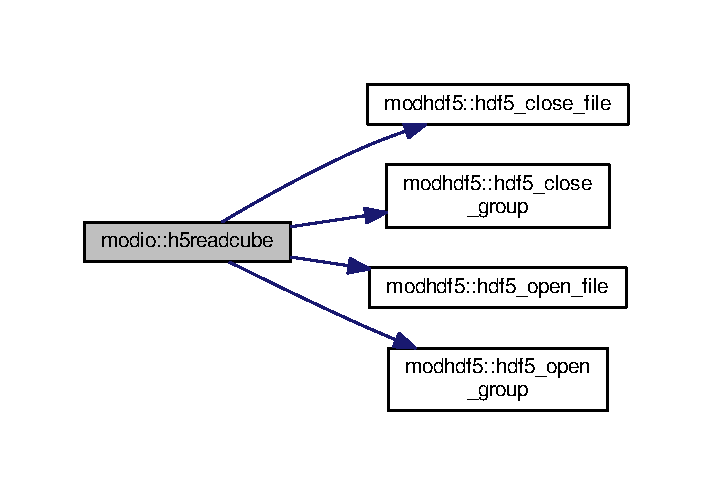
\includegraphics[width=342pt]{classmodio_a92f73643cbd1d8b16e0c29d683a147e0_cgraph}
\end{center}
\end{figure}




Here is the caller graph for this function\-:\nopagebreak
\begin{figure}[H]
\begin{center}
\leavevmode
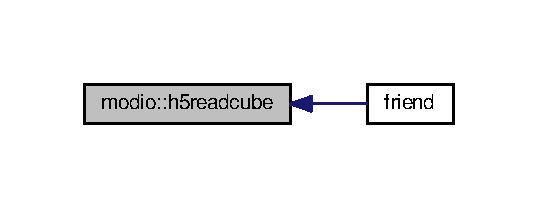
\includegraphics[width=258pt]{classmodio_a92f73643cbd1d8b16e0c29d683a147e0_icgraph}
\end{center}
\end{figure}


\hypertarget{classmodio_a0d3522f20c353a57b002c3120bc266f2}{\index{modio@{modio}!h5readmap@{h5readmap}}
\index{h5readmap@{h5readmap}!modio@{modio}}
\subsubsection[{h5readmap}]{\setlength{\rightskip}{0pt plus 5cm}subroutine modio\-::h5readmap (
\begin{DoxyParamCaption}
{}
\end{DoxyParamCaption}
)}}\label{classmodio_a0d3522f20c353a57b002c3120bc266f2}


This subroutine reads the map file. 



Definition at line 225 of file modio.\-f90.



References modhdf5\-::hdf5\-\_\-close\-\_\-file(), modhdf5\-::hdf5\-\_\-close\-\_\-group(), modhdf5\-::hdf5\-\_\-open\-\_\-file(), modhdf5\-::hdf5\-\_\-open\-\_\-group(), and modmpicom\-::settopology().



Here is the call graph for this function\-:\nopagebreak
\begin{figure}[H]
\begin{center}
\leavevmode
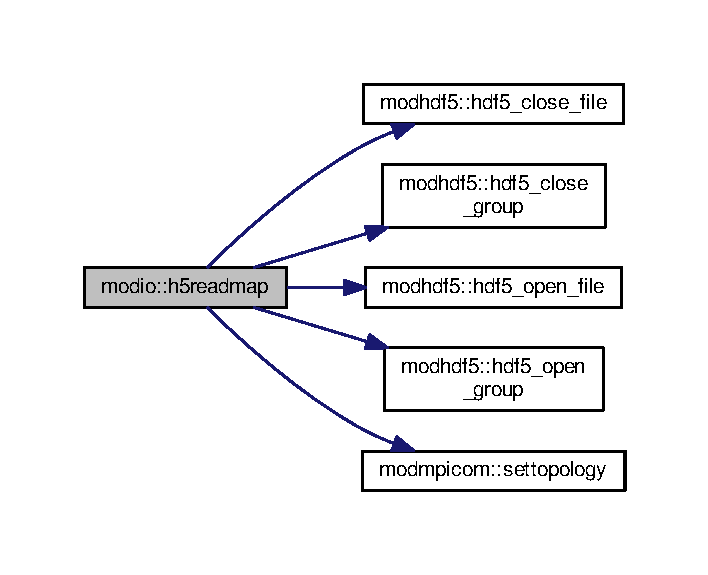
\includegraphics[width=340pt]{classmodio_a0d3522f20c353a57b002c3120bc266f2_cgraph}
\end{center}
\end{figure}




Here is the caller graph for this function\-:\nopagebreak
\begin{figure}[H]
\begin{center}
\leavevmode
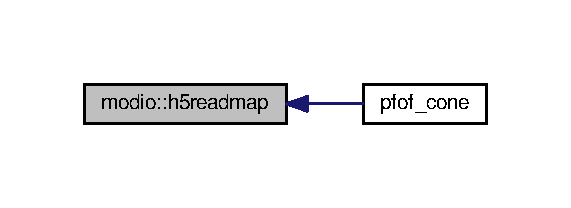
\includegraphics[width=274pt]{classmodio_a0d3522f20c353a57b002c3120bc266f2_icgraph}
\end{center}
\end{figure}


\hypertarget{classmodio_a8f70f66bd5285c807b17e0c89a6e0e4a}{\index{modio@{modio}!h5readparticles@{h5readparticles}}
\index{h5readparticles@{h5readparticles}!modio@{modio}}
\subsubsection[{h5readparticles}]{\setlength{\rightskip}{0pt plus 5cm}subroutine modio\-::h5readparticles (
\begin{DoxyParamCaption}
{}
\end{DoxyParamCaption}
)}}\label{classmodio_a8f70f66bd5285c807b17e0c89a6e0e4a}


This subroutine reads the particles from the shell files. 



Definition at line 288 of file modio.\-f90.



References modhdf5\-::hdf5\-\_\-close\-\_\-file(), modhdf5\-::hdf5\-\_\-close\-\_\-group(), modhdf5\-::hdf5\-\_\-open\-\_\-file(), and modhdf5\-::hdf5\-\_\-open\-\_\-group().



Here is the call graph for this function\-:\nopagebreak
\begin{figure}[H]
\begin{center}
\leavevmode
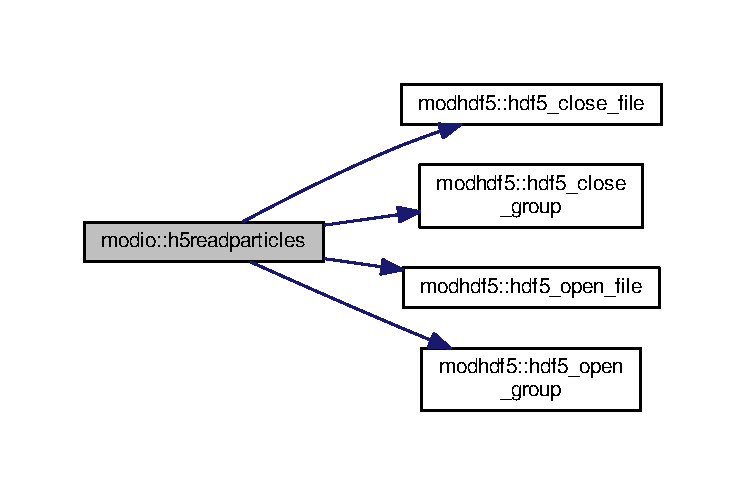
\includegraphics[width=350pt]{classmodio_a8f70f66bd5285c807b17e0c89a6e0e4a_cgraph}
\end{center}
\end{figure}




Here is the caller graph for this function\-:\nopagebreak
\begin{figure}[H]
\begin{center}
\leavevmode
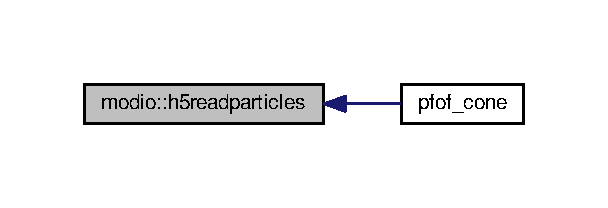
\includegraphics[width=292pt]{classmodio_a8f70f66bd5285c807b17e0c89a6e0e4a_icgraph}
\end{center}
\end{figure}


\hypertarget{classmodio_a5f1cc94eaee9d1f4f7bdca4cb63ee5bc}{\index{modio@{modio}!h5readshellinfo@{h5readshellinfo}}
\index{h5readshellinfo@{h5readshellinfo}!modio@{modio}}
\subsubsection[{h5readshellinfo}]{\setlength{\rightskip}{0pt plus 5cm}subroutine modio\-::h5readshellinfo (
\begin{DoxyParamCaption}
{}
\end{DoxyParamCaption}
)}}\label{classmodio_a5f1cc94eaee9d1f4f7bdca4cb63ee5bc}


This subroutine reads the cone size and the number of particles in each cubic group from each shell file, then writes an index of the cubes found in each shell file. 



Definition at line 109 of file modio.\-f90.



References modhdf5\-::hdf5\-\_\-close\-\_\-file(), and modhdf5\-::hdf5\-\_\-open\-\_\-file().



Here is the call graph for this function\-:\nopagebreak
\begin{figure}[H]
\begin{center}
\leavevmode
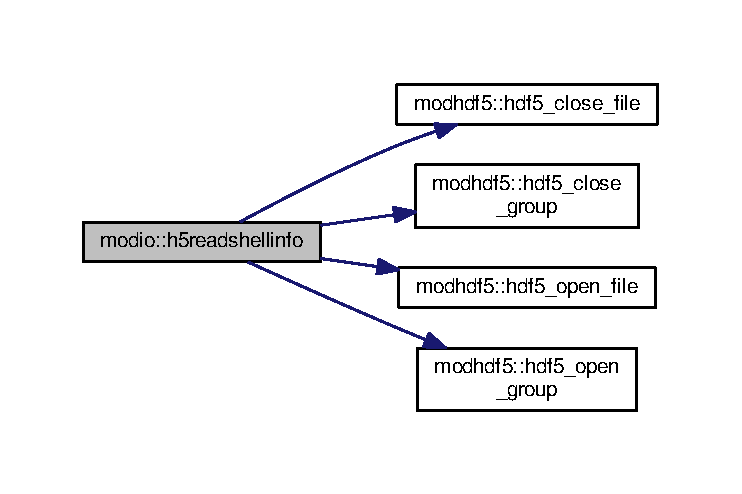
\includegraphics[width=350pt]{classmodio_a5f1cc94eaee9d1f4f7bdca4cb63ee5bc_cgraph}
\end{center}
\end{figure}




Here is the caller graph for this function\-:\nopagebreak
\begin{figure}[H]
\begin{center}
\leavevmode
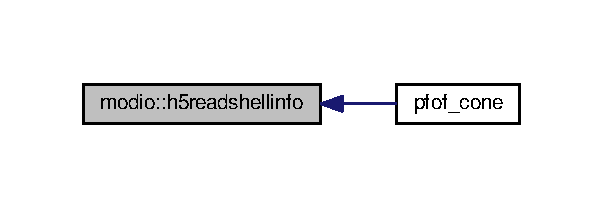
\includegraphics[width=290pt]{classmodio_a5f1cc94eaee9d1f4f7bdca4cb63ee5bc_icgraph}
\end{center}
\end{figure}


\hypertarget{classmodio_a52cdc31734affd194230ed16510dae68}{\index{modio@{modio}!h5writecube@{h5writecube}}
\index{h5writecube@{h5writecube}!modio@{modio}}
\subsubsection[{h5writecube}]{\setlength{\rightskip}{0pt plus 5cm}subroutine modio\-::h5writecube (
\begin{DoxyParamCaption}
{}
\end{DoxyParamCaption}
)}}\label{classmodio_a52cdc31734affd194230ed16510dae68}


This subroutine writes the position, velocity and id of each particle on the process in a hdf5 file. One file is written per M\-P\-I process. 



Definition at line 718 of file modio.\-f90.



References modhdf5\-::hdf5\-\_\-close\-\_\-file(), modhdf5\-::hdf5\-\_\-close\-\_\-group(), modhdf5\-::hdf5\-\_\-create\-\_\-file(), modhdf5\-::hdf5\-\_\-open\-\_\-group(), and modxdmf\-::writesinglecubexdmf().



Here is the call graph for this function\-:\nopagebreak
\begin{figure}[H]
\begin{center}
\leavevmode
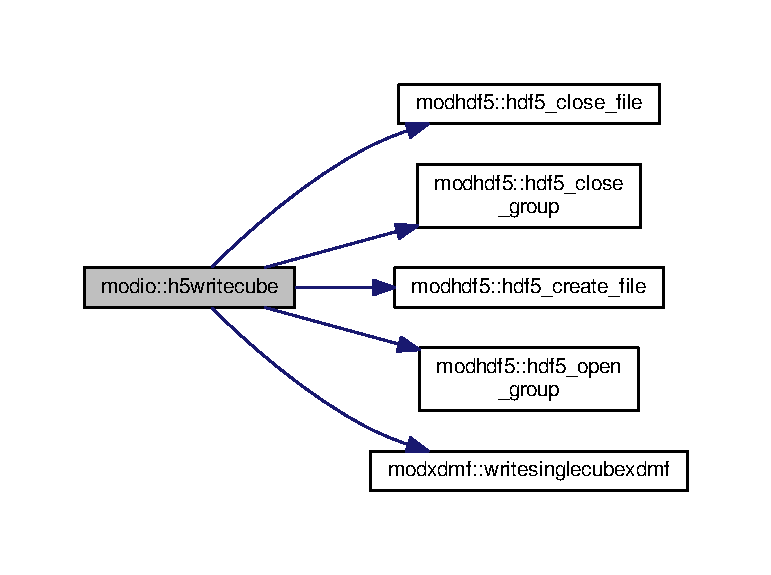
\includegraphics[width=350pt]{classmodio_a52cdc31734affd194230ed16510dae68_cgraph}
\end{center}
\end{figure}




Here is the caller graph for this function\-:\nopagebreak
\begin{figure}[H]
\begin{center}
\leavevmode
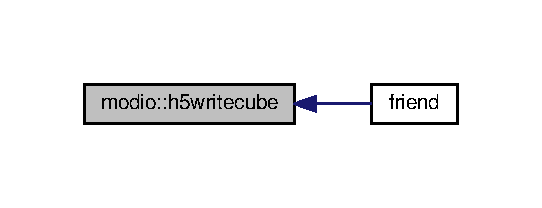
\includegraphics[width=260pt]{classmodio_a52cdc31734affd194230ed16510dae68_icgraph}
\end{center}
\end{figure}


\hypertarget{classmodio_a538e3b0c56f785106907880cb1e359b1}{\index{modio@{modio}!mpih5readcube@{mpih5readcube}}
\index{mpih5readcube@{mpih5readcube}!modio@{modio}}
\subsubsection[{mpih5readcube}]{\setlength{\rightskip}{0pt plus 5cm}subroutine modio\-::mpih5readcube (
\begin{DoxyParamCaption}
{}
\end{DoxyParamCaption}
)}}\label{classmodio_a538e3b0c56f785106907880cb1e359b1}


Definition at line 1332 of file modio.\-f90.



References modhdf5\-::hdf5\-\_\-close\-\_\-file(), modhdf5\-::hdf5\-\_\-close\-\_\-group(), modhdf5\-::hdf5\-\_\-open\-\_\-group(), and modhdf5\-::hdf5\-\_\-open\-\_\-mpi\-\_\-file().



Here is the call graph for this function\-:\nopagebreak
\begin{figure}[H]
\begin{center}
\leavevmode
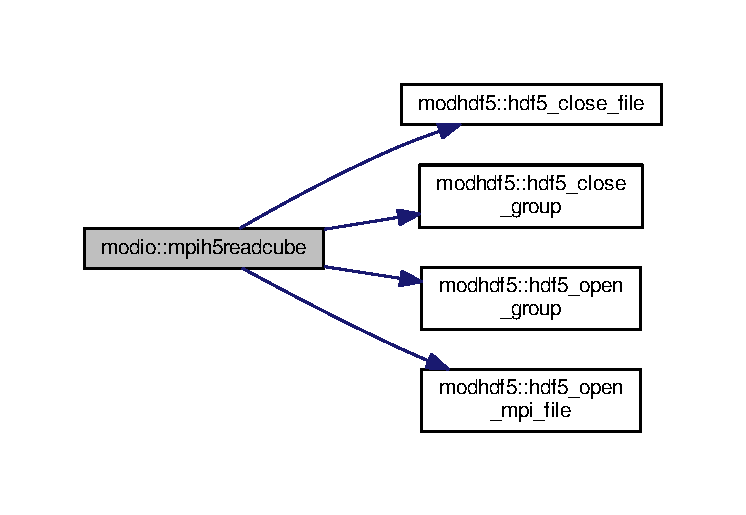
\includegraphics[width=350pt]{classmodio_a538e3b0c56f785106907880cb1e359b1_cgraph}
\end{center}
\end{figure}




Here is the caller graph for this function\-:\nopagebreak
\begin{figure}[H]
\begin{center}
\leavevmode
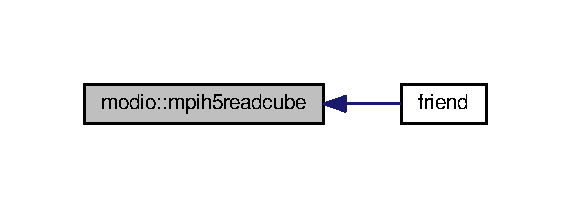
\includegraphics[width=274pt]{classmodio_a538e3b0c56f785106907880cb1e359b1_icgraph}
\end{center}
\end{figure}


\hypertarget{classmodio_af1c4604ad1d5c38063a516fe6ef6756d}{\index{modio@{modio}!mpih5writecube@{mpih5writecube}}
\index{mpih5writecube@{mpih5writecube}!modio@{modio}}
\subsubsection[{mpih5writecube}]{\setlength{\rightskip}{0pt plus 5cm}subroutine modio\-::mpih5writecube (
\begin{DoxyParamCaption}
{}
\end{DoxyParamCaption}
)}}\label{classmodio_af1c4604ad1d5c38063a516fe6ef6756d}


This subroutine writes the position, the velocity and the id of each particle on the process in a hdf5 file. The particles are gathered. 



Definition at line 1091 of file modio.\-f90.



References modhdf5\-::hdf5\-\_\-close\-\_\-group(), modhdf5\-::hdf5\-\_\-close\-\_\-mpi\-\_\-file(), modhdf5\-::hdf5\-\_\-create\-\_\-mpi\-\_\-file(), and modhdf5\-::hdf5\-\_\-open\-\_\-group().



Here is the call graph for this function\-:\nopagebreak
\begin{figure}[H]
\begin{center}
\leavevmode
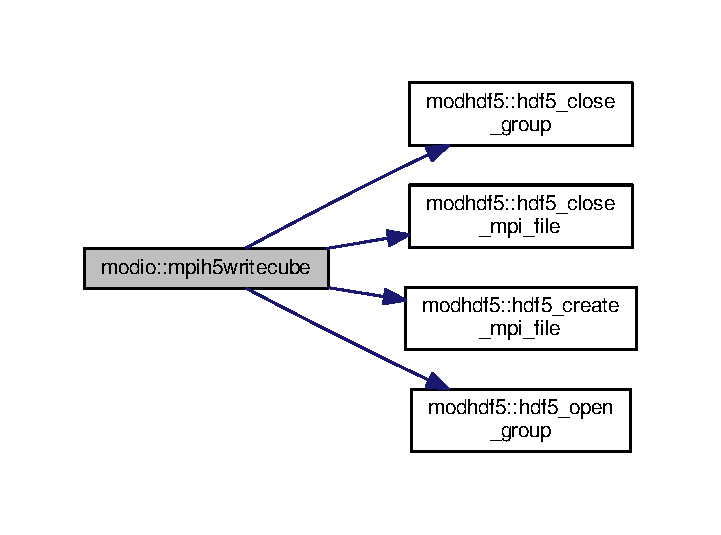
\includegraphics[width=346pt]{classmodio_af1c4604ad1d5c38063a516fe6ef6756d_cgraph}
\end{center}
\end{figure}




Here is the caller graph for this function\-:\nopagebreak
\begin{figure}[H]
\begin{center}
\leavevmode
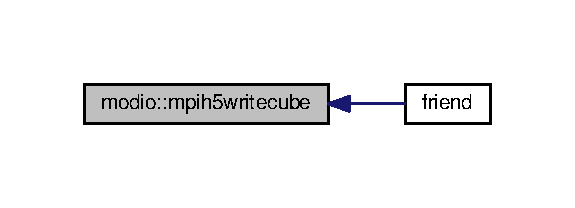
\includegraphics[width=276pt]{classmodio_af1c4604ad1d5c38063a516fe6ef6756d_icgraph}
\end{center}
\end{figure}


\hypertarget{classmodio_a663de68512ba066cd881ea37f378f6a8}{\index{modio@{modio}!outputcube@{outputcube}}
\index{outputcube@{outputcube}!modio@{modio}}
\subsubsection[{outputcube}]{\setlength{\rightskip}{0pt plus 5cm}subroutine modio\-::outputcube (
\begin{DoxyParamCaption}
{}
\end{DoxyParamCaption}
)}}\label{classmodio_a663de68512ba066cd881ea37f378f6a8}


This subroutine writes binary cube files. 



Definition at line 615 of file modio.\-f90.



Here is the caller graph for this function\-:\nopagebreak
\begin{figure}[H]
\begin{center}
\leavevmode
\includegraphics[width=256pt]{classmodio_a663de68512ba066cd881ea37f378f6a8_icgraph}
\end{center}
\end{figure}


\hypertarget{classmodio_a7bb73858f091ddd46631bcb29022f803}{\index{modio@{modio}!ramses\-\_\-lecture@{ramses\-\_\-lecture}}
\index{ramses\-\_\-lecture@{ramses\-\_\-lecture}!modio@{modio}}
\subsubsection[{ramses\-\_\-lecture}]{\setlength{\rightskip}{0pt plus 5cm}subroutine modio\-::ramses\-\_\-lecture (
\begin{DoxyParamCaption}
{}
\end{DoxyParamCaption}
)}}\label{classmodio_a7bb73858f091ddd46631bcb29022f803}


This subroutine reads the particles files created by R\-A\-M\-S\-E\-S that p\-F\-O\-F has to analyze. 



Definition at line 201 of file modio.\-f90.



References modmpicom\-::emergencystop().



Here is the call graph for this function\-:\nopagebreak
\begin{figure}[H]
\begin{center}
\leavevmode
\includegraphics[width=350pt]{classmodio_a7bb73858f091ddd46631bcb29022f803_cgraph}
\end{center}
\end{figure}




Here is the caller graph for this function\-:\nopagebreak
\begin{figure}[H]
\begin{center}
\leavevmode
\includegraphics[width=274pt]{classmodio_a7bb73858f091ddd46631bcb29022f803_icgraph}
\end{center}
\end{figure}


\hypertarget{classmodio_aa5e6b5f45cf8cfc091e8e7ff25a97c68}{\index{modio@{modio}!readparameters@{readparameters}}
\index{readparameters@{readparameters}!modio@{modio}}
\subsubsection[{readparameters}]{\setlength{\rightskip}{0pt plus 5cm}subroutine modio\-::readparameters (
\begin{DoxyParamCaption}
{}
\end{DoxyParamCaption}
)}}\label{classmodio_aa5e6b5f45cf8cfc091e8e7ff25a97c68}


This subroutine reads the input parameters from pfof.\-nml file (default name) with process 0 and broadcasts them to every processes. 



Definition at line 50 of file modio.\-f90.



References modmpicom\-::bcastparam().



Here is the call graph for this function\-:\nopagebreak
\begin{figure}[H]
\begin{center}
\leavevmode
\includegraphics[width=350pt]{classmodio_aa5e6b5f45cf8cfc091e8e7ff25a97c68_cgraph}
\end{center}
\end{figure}




Here is the caller graph for this function\-:\nopagebreak
\begin{figure}[H]
\begin{center}
\leavevmode
\includegraphics[width=292pt]{classmodio_aa5e6b5f45cf8cfc091e8e7ff25a97c68_icgraph}
\end{center}
\end{figure}


\hypertarget{classmodio_aa5e6b5f45cf8cfc091e8e7ff25a97c68}{\index{modio@{modio}!readparameters@{readparameters}}
\index{readparameters@{readparameters}!modio@{modio}}
\subsubsection[{readparameters}]{\setlength{\rightskip}{0pt plus 5cm}subroutine modio\-::readparameters (
\begin{DoxyParamCaption}
{}
\end{DoxyParamCaption}
)}}\label{classmodio_aa5e6b5f45cf8cfc091e8e7ff25a97c68}


This subroutine reads the parameters from the file pfof\-\_\-cone.\-nml. 



Definition at line 52 of file modio.\-f90.



References modmpicom\-::bcastparam().



Here is the call graph for this function\-:\nopagebreak
\begin{figure}[H]
\begin{center}
\leavevmode
\includegraphics[width=350pt]{classmodio_aa5e6b5f45cf8cfc091e8e7ff25a97c68_cgraph}
\end{center}
\end{figure}


\hypertarget{classmodio_aefab9476e94da81a75351dbeee74e623}{\index{modio@{modio}!title@{title}}
\index{title@{title}!modio@{modio}}
\subsubsection[{title}]{\setlength{\rightskip}{0pt plus 5cm}subroutine modio\-::title (
\begin{DoxyParamCaption}
{}
\end{DoxyParamCaption}
)}}\label{classmodio_aefab9476e94da81a75351dbeee74e623}


Definition at line 15 of file modio.\-f90.



Here is the caller graph for this function\-:\nopagebreak
\begin{figure}[H]
\begin{center}
\leavevmode
\includegraphics[width=242pt]{classmodio_aefab9476e94da81a75351dbeee74e623_icgraph}
\end{center}
\end{figure}


\hypertarget{classmodio_aefab9476e94da81a75351dbeee74e623}{\index{modio@{modio}!title@{title}}
\index{title@{title}!modio@{modio}}
\subsubsection[{title}]{\setlength{\rightskip}{0pt plus 5cm}subroutine modio\-::title (
\begin{DoxyParamCaption}
{}
\end{DoxyParamCaption}
)}}\label{classmodio_aefab9476e94da81a75351dbeee74e623}


Definition at line 21 of file modio.\-f90.

\hypertarget{classmodio_a943b18e88497f616e47f7be2047d269a}{\index{modio@{modio}!writehalomass@{writehalomass}}
\index{writehalomass@{writehalomass}!modio@{modio}}
\subsubsection[{writehalomass}]{\setlength{\rightskip}{0pt plus 5cm}subroutine modio\-::writehalomass (
\begin{DoxyParamCaption}
\item[{integer(kind=4), intent(in)}]{halo\-N\-B, }
\item[{integer(kind=4), dimension(halonb), intent(in)}]{halo\-Mass, }
\item[{real(kind=8), dimension(3,halonb), intent(in)}]{halocom\-Pos, }
\item[{integer(kind=pri), dimension(halonb), intent(in)}]{halo\-I\-D}
\end{DoxyParamCaption}
)}}\label{classmodio_a943b18e88497f616e47f7be2047d269a}


This subroutine writes binary files containing the mass, the id and the position of the center of mass for each halo found by p\-F\-O\-F. One file is written per process. 



Definition at line 644 of file modio.\-f90.



Here is the caller graph for this function\-:\nopagebreak
\begin{figure}[H]
\begin{center}
\leavevmode
\includegraphics[width=350pt]{classmodio_a943b18e88497f616e47f7be2047d269a_icgraph}
\end{center}
\end{figure}


\hypertarget{classmodio_ae7caa5bd1a32540628e11748a56626ae}{\index{modio@{modio}!writehalopart@{writehalopart}}
\index{writehalopart@{writehalopart}!modio@{modio}}
\subsubsection[{writehalopart}]{\setlength{\rightskip}{0pt plus 5cm}subroutine modio\-::writehalopart (
\begin{DoxyParamCaption}
\item[{integer(kind=4), intent(in)}]{halo\-N\-B, }
\item[{integer(kind=4), intent(in)}]{halopart\-N\-B, }
\item[{integer(kind=4), dimension(halonb), intent(in)}]{halo\-Mass, }
\item[{real (kind=4), dimension(3,halopartnb), intent(in)}]{halopart\-Pos, }
\item[{real (kind=4), dimension(3,halopartnb), intent(in)}]{halopart\-Vel, }
\item[{integer(kind=pri), dimension(halopartnb), intent(in)}]{halopart\-I\-D}
\end{DoxyParamCaption}
)}}\label{classmodio_ae7caa5bd1a32540628e11748a56626ae}


This subroutine writes binary files containing the position, the velocity and the id of each particle in each halo found by p\-F\-O\-F. One file is written per process. 



Definition at line 677 of file modio.\-f90.



Here is the caller graph for this function\-:\nopagebreak
\begin{figure}[H]
\begin{center}
\leavevmode
\includegraphics[width=350pt]{classmodio_ae7caa5bd1a32540628e11748a56626ae_icgraph}
\end{center}
\end{figure}


\hypertarget{classmodio_ae764b324dac1a0991a9643a54d47aa36}{\index{modio@{modio}!writeparameters@{writeparameters}}
\index{writeparameters@{writeparameters}!modio@{modio}}
\subsubsection[{writeparameters}]{\setlength{\rightskip}{0pt plus 5cm}subroutine modio\-::writeparameters (
\begin{DoxyParamCaption}
{}
\end{DoxyParamCaption}
)}}\label{classmodio_ae764b324dac1a0991a9643a54d47aa36}


This subroutine writes the input parameters in a .nml file, print them on screen and writes them in the .log file. It should be called only from process 0. 



Definition at line 97 of file modio.\-f90.



Here is the caller graph for this function\-:\nopagebreak
\begin{figure}[H]
\begin{center}
\leavevmode
\includegraphics[width=278pt]{classmodio_ae764b324dac1a0991a9643a54d47aa36_icgraph}
\end{center}
\end{figure}


\hypertarget{classmodio_a6ba64be35b401e31cd35f96ea50bb0c4}{\index{modio@{modio}!writetimings@{writetimings}}
\index{writetimings@{writetimings}!modio@{modio}}
\subsubsection[{writetimings}]{\setlength{\rightskip}{0pt plus 5cm}subroutine modio\-::writetimings (
\begin{DoxyParamCaption}
{}
\end{DoxyParamCaption}
)}}\label{classmodio_a6ba64be35b401e31cd35f96ea50bb0c4}


This subroutine writes timings in the log file and prints them on screen. It should be called only by process 0. It also closes the log file. 



Definition at line 158 of file modio.\-f90.



Here is the caller graph for this function\-:\nopagebreak
\begin{figure}[H]
\begin{center}
\leavevmode
\includegraphics[width=260pt]{classmodio_a6ba64be35b401e31cd35f96ea50bb0c4_icgraph}
\end{center}
\end{figure}




\subsection{Member Data Documentation}
\hypertarget{classmodio_a62b213d7b9f52071f903b877ee52c86b}{\index{modio@{modio}!ioerr@{ioerr}}
\index{ioerr@{ioerr}!modio@{modio}}
\subsubsection[{ioerr}]{\setlength{\rightskip}{0pt plus 5cm}integer(kind=4) modio\-::ioerr}}\label{classmodio_a62b213d7b9f52071f903b877ee52c86b}


Definition at line 17 of file modio.\-f90.

\hypertarget{classmodio_af7ac0e60c49f16bf08605237dd728508}{\index{modio@{modio}!ncube@{ncube}}
\index{ncube@{ncube}!modio@{modio}}
\subsubsection[{ncube}]{\setlength{\rightskip}{0pt plus 5cm}integer(kind=4) modio\-::ncube}}\label{classmodio_af7ac0e60c49f16bf08605237dd728508}


Definition at line 16 of file modio.\-f90.

\hypertarget{classmodio_a0bb05c9005df17b314c2a7e0f43e758c}{\index{modio@{modio}!npart\-\_\-tab@{npart\-\_\-tab}}
\index{npart\-\_\-tab@{npart\-\_\-tab}!modio@{modio}}
\subsubsection[{npart\-\_\-tab}]{\setlength{\rightskip}{0pt plus 5cm}integer(kind=4), dimension(\-:), allocatable modio\-::npart\-\_\-tab}}\label{classmodio_a0bb05c9005df17b314c2a7e0f43e758c}


Definition at line 18 of file modio.\-f90.



The documentation for this module was generated from the following file\-:\begin{DoxyCompactItemize}
\item 
/home/roy/\-Travail/\-Devel/\-Cosmologie/\-Pfof/trunk/pfof\-\_\-hdf5/src/\hyperlink{pfof__hdf5_2src_2modio_8f90}{modio.\-f90}\end{DoxyCompactItemize}

\hypertarget{classmodiocommons}{\section{modiocommons Module Reference}
\label{classmodiocommons}\index{modiocommons@{modiocommons}}
}


Common input/output procedures.  


\subsection*{Public Member Functions}
\begin{DoxyCompactItemize}
\item 
subroutine, public \hyperlink{classmodiocommons_aafba4b5ca834c55dd741c4040e971e5b}{h5write\-\_\-meta\-\_\-common} (file\-\_\-id, codename, npart)
\begin{DoxyCompactList}\small\item\em Write metadata common to every hdf5 ouput files of the pfof toolbox. \end{DoxyCompactList}\item 
subroutine, public \hyperlink{classmodiocommons_a6c7b87aedd57a36d2f5b643cb3fc7c12}{h5write\-\_\-meta\-\_\-pfof\-\_\-parameter} (file\-\_\-id, param\-\_\-pfof)
\begin{DoxyCompactList}\small\item\em Write pfof input parameters as metadata. \end{DoxyCompactList}\item 
subroutine, public \hyperlink{classmodiocommons_ac97d3aa8a31a87167c05ecbe841397cc}{h5write\-\_\-meta\-\_\-conecreator\-\_\-parameter} (file\-\_\-id, param\-\_\-cone)
\begin{DoxyCompactList}\small\item\em Write conecreator input parameters as metadata. \end{DoxyCompactList}\item 
subroutine, public \hyperlink{classmodiocommons_a88b4f4949433f00d81d86b9b1e031646}{h5write\-\_\-meta\-\_\-info\-\_\-ramses} (file\-\_\-id, inforamses)
\begin{DoxyCompactList}\small\item\em Write ramses info as metadata. \end{DoxyCompactList}\item 
subroutine, public \hyperlink{classmodiocommons_a7357bab67b152d137d4b2d43f30263e5}{h5write\-\_\-meta\-\_\-info\-\_\-cone} (file\-\_\-id, infocone)
\begin{DoxyCompactList}\small\item\em Write light cone info as metadata. \end{DoxyCompactList}\item 
subroutine, public \hyperlink{classmodiocommons_a1796f14ec35efbff3a4e692077c8bcf8}{h5read\-\_\-meta\-\_\-info\-\_\-ramses} (file\-\_\-id, inforamses)
\begin{DoxyCompactList}\small\item\em Read ramses info as metadata. \end{DoxyCompactList}\item 
subroutine, public \hyperlink{classmodiocommons_a23c194ca7b22b69dcf0bd2ea01b499d2}{h5read\-\_\-meta\-\_\-info\-\_\-cone} (file\-\_\-id, infocone)
\begin{DoxyCompactList}\small\item\em Read light cone info as metadata. \end{DoxyCompactList}\item 
subroutine, public \hyperlink{classmodiocommons_a05a591c82f587de8857aa9749786a9ed}{h5read\-\_\-meta\-\_\-pfof\-\_\-parameter} (file\-\_\-id, param\-\_\-pfof)
\begin{DoxyCompactList}\small\item\em Read pfof input parameters as metadata. \end{DoxyCompactList}\item 
subroutine, public \hyperlink{classmodiocommons_a5c8a5f561313ee8e555927237d405438}{h5read\-\_\-meta\-\_\-conecreator\-\_\-parameter} (file\-\_\-id, param\-\_\-cone)
\begin{DoxyCompactList}\small\item\em Read conecreator input parameters as metadata. \end{DoxyCompactList}\item 
subroutine, public \hyperlink{classmodiocommons_a653750d9160eb5e93a252a8da5aa09d6}{h5read\-\_\-meta\-\_\-common} (file\-\_\-id, common)
\begin{DoxyCompactList}\small\item\em Read metadata common to every hdf5 ouput files of the pfof toolbox. \end{DoxyCompactList}\end{DoxyCompactItemize}


\subsection{Detailed Description}
Common input/output procedures. 

Authors\-: F. Roy 

Definition at line 8 of file modiocommons.\-f90.



\subsection{Member Function/\-Subroutine Documentation}
\hypertarget{classmodiocommons_a653750d9160eb5e93a252a8da5aa09d6}{\index{modiocommons@{modiocommons}!h5read\-\_\-meta\-\_\-common@{h5read\-\_\-meta\-\_\-common}}
\index{h5read\-\_\-meta\-\_\-common@{h5read\-\_\-meta\-\_\-common}!modiocommons@{modiocommons}}
\subsubsection[{h5read\-\_\-meta\-\_\-common}]{\setlength{\rightskip}{0pt plus 5cm}subroutine, public modiocommons\-::h5read\-\_\-meta\-\_\-common (
\begin{DoxyParamCaption}
\item[{integer(kind=hid\-\_\-t), intent(in)}]{file\-\_\-id, }
\item[{type(type\-\_\-common\-\_\-metadata), intent(out)}]{common}
\end{DoxyParamCaption}
)}}\label{classmodiocommons_a653750d9160eb5e93a252a8da5aa09d6}


Read metadata common to every hdf5 ouput files of the pfof toolbox. 



Definition at line 1343 of file modiocommons.\-f90.



References modhdf5\-::hdf5\-\_\-close\-\_\-group(), and modhdf5\-::hdf5\-\_\-open\-\_\-group().



Here is the call graph for this function\-:\nopagebreak
\begin{figure}[H]
\begin{center}
\leavevmode
\includegraphics[width=346pt]{classmodiocommons_a653750d9160eb5e93a252a8da5aa09d6_cgraph}
\end{center}
\end{figure}




Here is the caller graph for this function\-:\nopagebreak
\begin{figure}[H]
\begin{center}
\leavevmode
\includegraphics[width=350pt]{classmodiocommons_a653750d9160eb5e93a252a8da5aa09d6_icgraph}
\end{center}
\end{figure}


\hypertarget{classmodiocommons_a5c8a5f561313ee8e555927237d405438}{\index{modiocommons@{modiocommons}!h5read\-\_\-meta\-\_\-conecreator\-\_\-parameter@{h5read\-\_\-meta\-\_\-conecreator\-\_\-parameter}}
\index{h5read\-\_\-meta\-\_\-conecreator\-\_\-parameter@{h5read\-\_\-meta\-\_\-conecreator\-\_\-parameter}!modiocommons@{modiocommons}}
\subsubsection[{h5read\-\_\-meta\-\_\-conecreator\-\_\-parameter}]{\setlength{\rightskip}{0pt plus 5cm}subroutine, public modiocommons\-::h5read\-\_\-meta\-\_\-conecreator\-\_\-parameter (
\begin{DoxyParamCaption}
\item[{integer(kind=hid\-\_\-t), intent(in)}]{file\-\_\-id, }
\item[{class(type\-\_\-parameter\-\_\-conecreator), intent(out)}]{param\-\_\-cone}
\end{DoxyParamCaption}
)}}\label{classmodiocommons_a5c8a5f561313ee8e555927237d405438}


Read conecreator input parameters as metadata. 



Definition at line 1245 of file modiocommons.\-f90.



References modhdf5\-::hdf5\-\_\-close\-\_\-group(), and modhdf5\-::hdf5\-\_\-open\-\_\-group().



Here is the call graph for this function\-:\nopagebreak
\begin{figure}[H]
\begin{center}
\leavevmode
\includegraphics[width=350pt]{classmodiocommons_a5c8a5f561313ee8e555927237d405438_cgraph}
\end{center}
\end{figure}


\hypertarget{classmodiocommons_a23c194ca7b22b69dcf0bd2ea01b499d2}{\index{modiocommons@{modiocommons}!h5read\-\_\-meta\-\_\-info\-\_\-cone@{h5read\-\_\-meta\-\_\-info\-\_\-cone}}
\index{h5read\-\_\-meta\-\_\-info\-\_\-cone@{h5read\-\_\-meta\-\_\-info\-\_\-cone}!modiocommons@{modiocommons}}
\subsubsection[{h5read\-\_\-meta\-\_\-info\-\_\-cone}]{\setlength{\rightskip}{0pt plus 5cm}subroutine, public modiocommons\-::h5read\-\_\-meta\-\_\-info\-\_\-cone (
\begin{DoxyParamCaption}
\item[{integer(kind=hid\-\_\-t), intent(in)}]{file\-\_\-id, }
\item[{class(type\-\_\-info\-\_\-cone), intent(out)}]{infocone}
\end{DoxyParamCaption}
)}}\label{classmodiocommons_a23c194ca7b22b69dcf0bd2ea01b499d2}


Read light cone info as metadata. 



Definition at line 918 of file modiocommons.\-f90.



References modhdf5\-::hdf5\-\_\-close\-\_\-group(), and modhdf5\-::hdf5\-\_\-open\-\_\-group().



Here is the call graph for this function\-:\nopagebreak
\begin{figure}[H]
\begin{center}
\leavevmode
\includegraphics[width=346pt]{classmodiocommons_a23c194ca7b22b69dcf0bd2ea01b499d2_cgraph}
\end{center}
\end{figure}




Here is the caller graph for this function\-:\nopagebreak
\begin{figure}[H]
\begin{center}
\leavevmode
\includegraphics[width=350pt]{classmodiocommons_a23c194ca7b22b69dcf0bd2ea01b499d2_icgraph}
\end{center}
\end{figure}


\hypertarget{classmodiocommons_a1796f14ec35efbff3a4e692077c8bcf8}{\index{modiocommons@{modiocommons}!h5read\-\_\-meta\-\_\-info\-\_\-ramses@{h5read\-\_\-meta\-\_\-info\-\_\-ramses}}
\index{h5read\-\_\-meta\-\_\-info\-\_\-ramses@{h5read\-\_\-meta\-\_\-info\-\_\-ramses}!modiocommons@{modiocommons}}
\subsubsection[{h5read\-\_\-meta\-\_\-info\-\_\-ramses}]{\setlength{\rightskip}{0pt plus 5cm}subroutine, public modiocommons\-::h5read\-\_\-meta\-\_\-info\-\_\-ramses (
\begin{DoxyParamCaption}
\item[{integer(kind=hid\-\_\-t), intent(in)}]{file\-\_\-id, }
\item[{type(type\-\_\-info\-\_\-ramses), intent(out)}]{inforamses}
\end{DoxyParamCaption}
)}}\label{classmodiocommons_a1796f14ec35efbff3a4e692077c8bcf8}


Read ramses info as metadata. 



Definition at line 839 of file modiocommons.\-f90.



References modhdf5\-::hdf5\-\_\-close\-\_\-group(), and modhdf5\-::hdf5\-\_\-open\-\_\-group().



Here is the call graph for this function\-:\nopagebreak
\begin{figure}[H]
\begin{center}
\leavevmode
\includegraphics[width=346pt]{classmodiocommons_a1796f14ec35efbff3a4e692077c8bcf8_cgraph}
\end{center}
\end{figure}




Here is the caller graph for this function\-:\nopagebreak
\begin{figure}[H]
\begin{center}
\leavevmode
\includegraphics[width=350pt]{classmodiocommons_a1796f14ec35efbff3a4e692077c8bcf8_icgraph}
\end{center}
\end{figure}


\hypertarget{classmodiocommons_a05a591c82f587de8857aa9749786a9ed}{\index{modiocommons@{modiocommons}!h5read\-\_\-meta\-\_\-pfof\-\_\-parameter@{h5read\-\_\-meta\-\_\-pfof\-\_\-parameter}}
\index{h5read\-\_\-meta\-\_\-pfof\-\_\-parameter@{h5read\-\_\-meta\-\_\-pfof\-\_\-parameter}!modiocommons@{modiocommons}}
\subsubsection[{h5read\-\_\-meta\-\_\-pfof\-\_\-parameter}]{\setlength{\rightskip}{0pt plus 5cm}subroutine, public modiocommons\-::h5read\-\_\-meta\-\_\-pfof\-\_\-parameter (
\begin{DoxyParamCaption}
\item[{integer(kind=hid\-\_\-t), intent(in)}]{file\-\_\-id, }
\item[{class(type\-\_\-parameter\-\_\-pfof), intent(out)}]{param\-\_\-pfof}
\end{DoxyParamCaption}
)}}\label{classmodiocommons_a05a591c82f587de8857aa9749786a9ed}


Read pfof input parameters as metadata. 



Definition at line 1073 of file modiocommons.\-f90.



References modhdf5\-::hdf5\-\_\-close\-\_\-group(), and modhdf5\-::hdf5\-\_\-open\-\_\-group().



Here is the call graph for this function\-:\nopagebreak
\begin{figure}[H]
\begin{center}
\leavevmode
\includegraphics[width=346pt]{classmodiocommons_a05a591c82f587de8857aa9749786a9ed_cgraph}
\end{center}
\end{figure}




Here is the caller graph for this function\-:\nopagebreak
\begin{figure}[H]
\begin{center}
\leavevmode
\includegraphics[width=346pt]{classmodiocommons_a05a591c82f587de8857aa9749786a9ed_icgraph}
\end{center}
\end{figure}


\hypertarget{classmodiocommons_aafba4b5ca834c55dd741c4040e971e5b}{\index{modiocommons@{modiocommons}!h5write\-\_\-meta\-\_\-common@{h5write\-\_\-meta\-\_\-common}}
\index{h5write\-\_\-meta\-\_\-common@{h5write\-\_\-meta\-\_\-common}!modiocommons@{modiocommons}}
\subsubsection[{h5write\-\_\-meta\-\_\-common}]{\setlength{\rightskip}{0pt plus 5cm}subroutine, public modiocommons\-::h5write\-\_\-meta\-\_\-common (
\begin{DoxyParamCaption}
\item[{integer(kind=hid\-\_\-t), intent(in)}]{file\-\_\-id, }
\item[{character(len=h5strlen), intent(in)}]{codename, }
\item[{integer(kind=8), intent(in)}]{npart}
\end{DoxyParamCaption}
)}}\label{classmodiocommons_aafba4b5ca834c55dd741c4040e971e5b}


Write metadata common to every hdf5 ouput files of the pfof toolbox. 



Definition at line 30 of file modiocommons.\-f90.



References modhdf5\-::hdf5\-\_\-close\-\_\-group(), and modhdf5\-::hdf5\-\_\-open\-\_\-group().



Here is the call graph for this function\-:\nopagebreak
\begin{figure}[H]
\begin{center}
\leavevmode
\includegraphics[width=348pt]{classmodiocommons_aafba4b5ca834c55dd741c4040e971e5b_cgraph}
\end{center}
\end{figure}




Here is the caller graph for this function\-:\nopagebreak
\begin{figure}[H]
\begin{center}
\leavevmode
\includegraphics[width=350pt]{classmodiocommons_aafba4b5ca834c55dd741c4040e971e5b_icgraph}
\end{center}
\end{figure}


\hypertarget{classmodiocommons_ac97d3aa8a31a87167c05ecbe841397cc}{\index{modiocommons@{modiocommons}!h5write\-\_\-meta\-\_\-conecreator\-\_\-parameter@{h5write\-\_\-meta\-\_\-conecreator\-\_\-parameter}}
\index{h5write\-\_\-meta\-\_\-conecreator\-\_\-parameter@{h5write\-\_\-meta\-\_\-conecreator\-\_\-parameter}!modiocommons@{modiocommons}}
\subsubsection[{h5write\-\_\-meta\-\_\-conecreator\-\_\-parameter}]{\setlength{\rightskip}{0pt plus 5cm}subroutine, public modiocommons\-::h5write\-\_\-meta\-\_\-conecreator\-\_\-parameter (
\begin{DoxyParamCaption}
\item[{integer(kind=hid\-\_\-t), intent(in)}]{file\-\_\-id, }
\item[{class(type\-\_\-parameter\-\_\-conecreator), intent(in)}]{param\-\_\-cone}
\end{DoxyParamCaption}
)}}\label{classmodiocommons_ac97d3aa8a31a87167c05ecbe841397cc}


Write conecreator input parameters as metadata. 



Definition at line 279 of file modiocommons.\-f90.



References modhdf5\-::hdf5\-\_\-close\-\_\-group(), modhdf5\-::hdf5\-\_\-create\-\_\-group(), and modhdf5\-::hdf5\-\_\-open\-\_\-group().



Here is the call graph for this function\-:\nopagebreak
\begin{figure}[H]
\begin{center}
\leavevmode
\includegraphics[width=350pt]{classmodiocommons_ac97d3aa8a31a87167c05ecbe841397cc_cgraph}
\end{center}
\end{figure}




Here is the caller graph for this function\-:\nopagebreak
\begin{figure}[H]
\begin{center}
\leavevmode
\includegraphics[width=350pt]{classmodiocommons_ac97d3aa8a31a87167c05ecbe841397cc_icgraph}
\end{center}
\end{figure}


\hypertarget{classmodiocommons_a7357bab67b152d137d4b2d43f30263e5}{\index{modiocommons@{modiocommons}!h5write\-\_\-meta\-\_\-info\-\_\-cone@{h5write\-\_\-meta\-\_\-info\-\_\-cone}}
\index{h5write\-\_\-meta\-\_\-info\-\_\-cone@{h5write\-\_\-meta\-\_\-info\-\_\-cone}!modiocommons@{modiocommons}}
\subsubsection[{h5write\-\_\-meta\-\_\-info\-\_\-cone}]{\setlength{\rightskip}{0pt plus 5cm}subroutine, public modiocommons\-::h5write\-\_\-meta\-\_\-info\-\_\-cone (
\begin{DoxyParamCaption}
\item[{integer(kind=hid\-\_\-t), intent(in)}]{file\-\_\-id, }
\item[{class(type\-\_\-info\-\_\-cone), intent(in)}]{infocone}
\end{DoxyParamCaption}
)}}\label{classmodiocommons_a7357bab67b152d137d4b2d43f30263e5}


Write light cone info as metadata. 



Definition at line 458 of file modiocommons.\-f90.



References modhdf5\-::hdf5\-\_\-close\-\_\-group(), modhdf5\-::hdf5\-\_\-create\-\_\-group(), and modhdf5\-::hdf5\-\_\-open\-\_\-group().



Here is the call graph for this function\-:\nopagebreak
\begin{figure}[H]
\begin{center}
\leavevmode
\includegraphics[width=350pt]{classmodiocommons_a7357bab67b152d137d4b2d43f30263e5_cgraph}
\end{center}
\end{figure}




Here is the caller graph for this function\-:\nopagebreak
\begin{figure}[H]
\begin{center}
\leavevmode
\includegraphics[width=350pt]{classmodiocommons_a7357bab67b152d137d4b2d43f30263e5_icgraph}
\end{center}
\end{figure}


\hypertarget{classmodiocommons_a88b4f4949433f00d81d86b9b1e031646}{\index{modiocommons@{modiocommons}!h5write\-\_\-meta\-\_\-info\-\_\-ramses@{h5write\-\_\-meta\-\_\-info\-\_\-ramses}}
\index{h5write\-\_\-meta\-\_\-info\-\_\-ramses@{h5write\-\_\-meta\-\_\-info\-\_\-ramses}!modiocommons@{modiocommons}}
\subsubsection[{h5write\-\_\-meta\-\_\-info\-\_\-ramses}]{\setlength{\rightskip}{0pt plus 5cm}subroutine, public modiocommons\-::h5write\-\_\-meta\-\_\-info\-\_\-ramses (
\begin{DoxyParamCaption}
\item[{integer(kind=hid\-\_\-t), intent(in)}]{file\-\_\-id, }
\item[{type(type\-\_\-info\-\_\-ramses), intent(in)}]{inforamses}
\end{DoxyParamCaption}
)}}\label{classmodiocommons_a88b4f4949433f00d81d86b9b1e031646}


Write ramses info as metadata. 



Definition at line 378 of file modiocommons.\-f90.



References modhdf5\-::hdf5\-\_\-close\-\_\-group(), modhdf5\-::hdf5\-\_\-create\-\_\-group(), and modhdf5\-::hdf5\-\_\-open\-\_\-group().



Here is the call graph for this function\-:\nopagebreak
\begin{figure}[H]
\begin{center}
\leavevmode
\includegraphics[width=350pt]{classmodiocommons_a88b4f4949433f00d81d86b9b1e031646_cgraph}
\end{center}
\end{figure}




Here is the caller graph for this function\-:\nopagebreak
\begin{figure}[H]
\begin{center}
\leavevmode
\includegraphics[width=350pt]{classmodiocommons_a88b4f4949433f00d81d86b9b1e031646_icgraph}
\end{center}
\end{figure}


\hypertarget{classmodiocommons_a6c7b87aedd57a36d2f5b643cb3fc7c12}{\index{modiocommons@{modiocommons}!h5write\-\_\-meta\-\_\-pfof\-\_\-parameter@{h5write\-\_\-meta\-\_\-pfof\-\_\-parameter}}
\index{h5write\-\_\-meta\-\_\-pfof\-\_\-parameter@{h5write\-\_\-meta\-\_\-pfof\-\_\-parameter}!modiocommons@{modiocommons}}
\subsubsection[{h5write\-\_\-meta\-\_\-pfof\-\_\-parameter}]{\setlength{\rightskip}{0pt plus 5cm}subroutine, public modiocommons\-::h5write\-\_\-meta\-\_\-pfof\-\_\-parameter (
\begin{DoxyParamCaption}
\item[{integer(kind=hid\-\_\-t), intent(in)}]{file\-\_\-id, }
\item[{class(type\-\_\-parameter\-\_\-pfof), intent(in)}]{param\-\_\-pfof}
\end{DoxyParamCaption}
)}}\label{classmodiocommons_a6c7b87aedd57a36d2f5b643cb3fc7c12}


Write pfof input parameters as metadata. 



Definition at line 82 of file modiocommons.\-f90.



References modhdf5\-::hdf5\-\_\-close\-\_\-group(), modhdf5\-::hdf5\-\_\-create\-\_\-group(), and modhdf5\-::hdf5\-\_\-open\-\_\-group().



Here is the call graph for this function\-:\nopagebreak
\begin{figure}[H]
\begin{center}
\leavevmode
\includegraphics[width=350pt]{classmodiocommons_a6c7b87aedd57a36d2f5b643cb3fc7c12_cgraph}
\end{center}
\end{figure}




Here is the caller graph for this function\-:\nopagebreak
\begin{figure}[H]
\begin{center}
\leavevmode
\includegraphics[width=350pt]{classmodiocommons_a6c7b87aedd57a36d2f5b643cb3fc7c12_icgraph}
\end{center}
\end{figure}




The documentation for this module was generated from the following file\-:\begin{DoxyCompactItemize}
\item 
/home/roy/\-Travail/\-Devel/\-Cosmologie/\-Pfof/branches/\-Modif\-Struct/common/src/\hyperlink{modiocommons_8f90}{modiocommons.\-f90}\end{DoxyCompactItemize}

\hypertarget{classmodmap}{\section{modmap Module Reference}
\label{classmodmap}\index{modmap@{modmap}}
}
\subsection*{Public Member Functions}
\begin{DoxyCompactItemize}
\item 
subroutine \hyperlink{classmodmap_a4dabe74fe33947e22abfde9897dff20b}{exploremap} ()
\item 
subroutine \hyperlink{classmodmap_af6328324bc6aaca47018ded5f4c8e8cb}{map} (factor)
\item 
subroutine \hyperlink{classmodmap_a61603fa7aecee06e2efaa0c647e35df6}{getnpfromshell} (factor, if, jf, kf, np)
\end{DoxyCompactItemize}
\subsection*{Public Attributes}
\begin{DoxyCompactItemize}
\item 
integer(kind=4) \hyperlink{classmodmap_a4c96661037ebd0e043cf2967b7e94067}{fofgrid\-\_\-imin}
\item 
integer(kind=4) \hyperlink{classmodmap_adf255364fd93d9af29d1f179bf50f5ba}{fofgrid\-\_\-imax}
\item 
integer(kind=4) \hyperlink{classmodmap_ac44fd964c6a2812634e903df91c5bcb6}{fofgrid\-\_\-jmin}
\item 
integer(kind=4) \hyperlink{classmodmap_a1644332b29d20583060c9316d8cd2fa1}{fofgrid\-\_\-jmax}
\item 
integer(kind=4) \hyperlink{classmodmap_ac4f40bdda34481044d92691776976abc}{fofgrid\-\_\-kmin}
\item 
integer(kind=4) \hyperlink{classmodmap_a7273a00ef7481fa382b6016d39a752e3}{fofgrid\-\_\-kmax}
\item 
integer(kind=4), dimension(\-:), \\*
allocatable \hyperlink{classmodmap_af68652ecce879493f3a84180017cccbd}{ict}
\end{DoxyCompactItemize}


\subsection{Detailed Description}


Definition at line 5 of file modmap.\-f90.



\subsection{Member Function/\-Subroutine Documentation}
\hypertarget{classmodmap_a4dabe74fe33947e22abfde9897dff20b}{\index{modmap@{modmap}!exploremap@{exploremap}}
\index{exploremap@{exploremap}!modmap@{modmap}}
\subsubsection[{exploremap}]{\setlength{\rightskip}{0pt plus 5cm}subroutine modmap\-::exploremap (
\begin{DoxyParamCaption}
{}
\end{DoxyParamCaption}
)}}\label{classmodmap_a4dabe74fe33947e22abfde9897dff20b}


Definition at line 20 of file modmap.\-f90.



References map().



Here is the call graph for this function\-:\nopagebreak
\begin{figure}[H]
\begin{center}
\leavevmode
\includegraphics[width=350pt]{classmodmap_a4dabe74fe33947e22abfde9897dff20b_cgraph}
\end{center}
\end{figure}




Here is the caller graph for this function\-:\nopagebreak
\begin{figure}[H]
\begin{center}
\leavevmode
\includegraphics[width=296pt]{classmodmap_a4dabe74fe33947e22abfde9897dff20b_icgraph}
\end{center}
\end{figure}


\hypertarget{classmodmap_a61603fa7aecee06e2efaa0c647e35df6}{\index{modmap@{modmap}!getnpfromshell@{getnpfromshell}}
\index{getnpfromshell@{getnpfromshell}!modmap@{modmap}}
\subsubsection[{getnpfromshell}]{\setlength{\rightskip}{0pt plus 5cm}subroutine modmap\-::getnpfromshell (
\begin{DoxyParamCaption}
\item[{integer(kind=4), intent(in)}]{factor, }
\item[{integer(kind=4), intent(in)}]{if, }
\item[{integer(kind=4), intent(in)}]{jf, }
\item[{integer(kind=4), intent(in)}]{kf, }
\item[{integer(kind=8), intent(out)}]{np}
\end{DoxyParamCaption}
)}}\label{classmodmap_a61603fa7aecee06e2efaa0c647e35df6}


Definition at line 339 of file modmap.\-f90.



Here is the caller graph for this function\-:\nopagebreak
\begin{figure}[H]
\begin{center}
\leavevmode
\includegraphics[width=350pt]{classmodmap_a61603fa7aecee06e2efaa0c647e35df6_icgraph}
\end{center}
\end{figure}


\hypertarget{classmodmap_af6328324bc6aaca47018ded5f4c8e8cb}{\index{modmap@{modmap}!map@{map}}
\index{map@{map}!modmap@{modmap}}
\subsubsection[{map}]{\setlength{\rightskip}{0pt plus 5cm}subroutine modmap\-::map (
\begin{DoxyParamCaption}
\item[{integer(kind=4), intent(in)}]{factor}
\end{DoxyParamCaption}
)}}\label{classmodmap_af6328324bc6aaca47018ded5f4c8e8cb}


Definition at line 53 of file modmap.\-f90.



References getnpfromshell(), and modio\-::h5writemap().



Here is the call graph for this function\-:\nopagebreak
\begin{figure}[H]
\begin{center}
\leavevmode
\includegraphics[width=350pt]{classmodmap_af6328324bc6aaca47018ded5f4c8e8cb_cgraph}
\end{center}
\end{figure}




Here is the caller graph for this function\-:\nopagebreak
\begin{figure}[H]
\begin{center}
\leavevmode
\includegraphics[width=350pt]{classmodmap_af6328324bc6aaca47018ded5f4c8e8cb_icgraph}
\end{center}
\end{figure}




\subsection{Member Data Documentation}
\hypertarget{classmodmap_adf255364fd93d9af29d1f179bf50f5ba}{\index{modmap@{modmap}!fofgrid\-\_\-imax@{fofgrid\-\_\-imax}}
\index{fofgrid\-\_\-imax@{fofgrid\-\_\-imax}!modmap@{modmap}}
\subsubsection[{fofgrid\-\_\-imax}]{\setlength{\rightskip}{0pt plus 5cm}integer(kind=4) modmap\-::fofgrid\-\_\-imax}}\label{classmodmap_adf255364fd93d9af29d1f179bf50f5ba}


Definition at line 11 of file modmap.\-f90.

\hypertarget{classmodmap_a4c96661037ebd0e043cf2967b7e94067}{\index{modmap@{modmap}!fofgrid\-\_\-imin@{fofgrid\-\_\-imin}}
\index{fofgrid\-\_\-imin@{fofgrid\-\_\-imin}!modmap@{modmap}}
\subsubsection[{fofgrid\-\_\-imin}]{\setlength{\rightskip}{0pt plus 5cm}integer(kind=4) modmap\-::fofgrid\-\_\-imin}}\label{classmodmap_a4c96661037ebd0e043cf2967b7e94067}


Definition at line 11 of file modmap.\-f90.

\hypertarget{classmodmap_a1644332b29d20583060c9316d8cd2fa1}{\index{modmap@{modmap}!fofgrid\-\_\-jmax@{fofgrid\-\_\-jmax}}
\index{fofgrid\-\_\-jmax@{fofgrid\-\_\-jmax}!modmap@{modmap}}
\subsubsection[{fofgrid\-\_\-jmax}]{\setlength{\rightskip}{0pt plus 5cm}integer(kind=4) modmap\-::fofgrid\-\_\-jmax}}\label{classmodmap_a1644332b29d20583060c9316d8cd2fa1}


Definition at line 12 of file modmap.\-f90.

\hypertarget{classmodmap_ac44fd964c6a2812634e903df91c5bcb6}{\index{modmap@{modmap}!fofgrid\-\_\-jmin@{fofgrid\-\_\-jmin}}
\index{fofgrid\-\_\-jmin@{fofgrid\-\_\-jmin}!modmap@{modmap}}
\subsubsection[{fofgrid\-\_\-jmin}]{\setlength{\rightskip}{0pt plus 5cm}integer(kind=4) modmap\-::fofgrid\-\_\-jmin}}\label{classmodmap_ac44fd964c6a2812634e903df91c5bcb6}


Definition at line 12 of file modmap.\-f90.

\hypertarget{classmodmap_a7273a00ef7481fa382b6016d39a752e3}{\index{modmap@{modmap}!fofgrid\-\_\-kmax@{fofgrid\-\_\-kmax}}
\index{fofgrid\-\_\-kmax@{fofgrid\-\_\-kmax}!modmap@{modmap}}
\subsubsection[{fofgrid\-\_\-kmax}]{\setlength{\rightskip}{0pt plus 5cm}integer(kind=4) modmap\-::fofgrid\-\_\-kmax}}\label{classmodmap_a7273a00ef7481fa382b6016d39a752e3}


Definition at line 13 of file modmap.\-f90.

\hypertarget{classmodmap_ac4f40bdda34481044d92691776976abc}{\index{modmap@{modmap}!fofgrid\-\_\-kmin@{fofgrid\-\_\-kmin}}
\index{fofgrid\-\_\-kmin@{fofgrid\-\_\-kmin}!modmap@{modmap}}
\subsubsection[{fofgrid\-\_\-kmin}]{\setlength{\rightskip}{0pt plus 5cm}integer(kind=4) modmap\-::fofgrid\-\_\-kmin}}\label{classmodmap_ac4f40bdda34481044d92691776976abc}


Definition at line 13 of file modmap.\-f90.

\hypertarget{classmodmap_af68652ecce879493f3a84180017cccbd}{\index{modmap@{modmap}!ict@{ict}}
\index{ict@{ict}!modmap@{modmap}}
\subsubsection[{ict}]{\setlength{\rightskip}{0pt plus 5cm}integer(kind=4), dimension(\-:), allocatable modmap\-::ict}}\label{classmodmap_af68652ecce879493f3a84180017cccbd}


Definition at line 14 of file modmap.\-f90.



The documentation for this module was generated from the following file\-:\begin{DoxyCompactItemize}
\item 
/home/roy/\-Travail/\-Devel/\-Cosmologie/\-Pfof/branches/\-Modif\-Struct/tools/conemapper/src/\hyperlink{modmap_8f90}{modmap.\-f90}\end{DoxyCompactItemize}

\hypertarget{classmodmpicom}{\section{modmpicom Module Reference}
\label{classmodmpicom}\index{modmpicom@{modmpicom}}
}


This module contains the subroutines and the variables used for M\-P\-I communications. Authors\-: F. Roy, V. Bouillot.  


\subsection*{Public Member Functions}
\begin{DoxyCompactItemize}
\item 
subroutine, public \hyperlink{classmodmpicom_a7cbb93c720bce9f56e7482758ab348c5}{setcommunicators} ()
\begin{DoxyCompactList}\small\item\em This subroutine creates the global cartesian grid of processes. It also creates the communicators used for the parallel hdf5 i/o if they are needed. \end{DoxyCompactList}\item 
subroutine, public \hyperlink{classmodmpicom_abc2ffa06e3665781143ba0241350b976}{settopology} ()
\begin{DoxyCompactList}\small\item\em This subroutine create a processes topology that maps the lightcone. \end{DoxyCompactList}\end{DoxyCompactItemize}
\subsection*{Public Attributes}
\begin{DoxyCompactItemize}
\item 
integer(kind=4), dimension(3), \\*
public \hyperlink{classmodmpicom_ab53b6d73e6ad2ed312af8e9fcacdcd39}{dims}
\begin{DoxyCompactList}\small\item\em dimensions of the processes grid \end{DoxyCompactList}\item 
integer(kind=4), public \hyperlink{classmodmpicom_a98a18237a2ccfdfdfd230104e90e9b5d}{mpicube}
\begin{DoxyCompactList}\small\item\em cartesian global communicator \end{DoxyCompactList}\item 
integer(kind=4), public \hyperlink{classmodmpicom_aa4714e524c20e853ca0d8eee443a3eaa}{mpisubcubewrite}
\begin{DoxyCompactList}\small\item\em local communicator used for hdf5 parallel output \end{DoxyCompactList}\item 
integer(kind=4), public \hyperlink{classmodmpicom_a0e30077f764b1d64af266f38546eb11b}{mpisubcuberead}
\begin{DoxyCompactList}\small\item\em local communicator used for hdf5 parallel input \end{DoxyCompactList}\item 
integer(kind=4), dimension(3), \\*
public \hyperlink{classmodmpicom_a82b7ffcc29d150ab9a64cbf53757feca}{cubecoord}
\begin{DoxyCompactList}\small\item\em coordinates of the process in the Mpi\-Cube communicator \end{DoxyCompactList}\item 
integer(kind=4), public \hyperlink{classmodmpicom_ac492fd7b2b0e1274ab259b5377a8a907}{commcolorwrite}
\begin{DoxyCompactList}\small\item\em parameter used to create the Mpi\-Sub\-Cube\-Write communicator \end{DoxyCompactList}\item 
integer(kind=4), public \hyperlink{classmodmpicom_ab58830af4e3abbec4491393d1f151ca8}{commcolorread}
\begin{DoxyCompactList}\small\item\em parameter used to create the Mpi\-Sub\-Cube\-Read communicator \end{DoxyCompactList}\item 
integer(kind=4), public \hyperlink{classmodmpicom_abebf60043baa916259ad148a0856c87a}{scprocidwrite}
\begin{DoxyCompactList}\small\item\em process id in the Mpi\-Sub\-Cube\-Write communicator \end{DoxyCompactList}\item 
integer(kind=4), public \hyperlink{classmodmpicom_af5dc4e2e2c054269623303e30bb81ee4}{scprocidread}
\begin{DoxyCompactList}\small\item\em process id in the Mpi\-Sub\-Cube\-Read communicator \end{DoxyCompactList}\item 
integer(kind=4) \hyperlink{classmodmpicom_a8281c8567826b44d76d7a801203c99a8}{scprocnbwrite}
\begin{DoxyCompactList}\small\item\em process number in the Mpi\-Sub\-Cube\-Write communicator \end{DoxyCompactList}\item 
integer(kind=4) \hyperlink{classmodmpicom_a8fde31beaf4b43228d7f93325630cefa}{scprocnbread}
\begin{DoxyCompactList}\small\item\em process number in the Mpi\-Sub\-Cube\-Read communicator \end{DoxyCompactList}\item 
logical(kind=4), dimension(3) \hyperlink{classmodmpicom_a0347e6d8a15028132a57953e6ff823a2}{periods}
\begin{DoxyCompactList}\small\item\em periodicity of the global cartesian processes grid \end{DoxyCompactList}\item 
integer(kind=4), dimension(3) \hyperlink{classmodmpicom_a533718abb8ce3f03b430dfbf9f821069}{cubecoord}
\begin{DoxyCompactList}\small\item\em coordinates of the process in the Mpi\-Cube communicator \end{DoxyCompactList}\end{DoxyCompactItemize}


\subsection{Detailed Description}
This module contains the subroutines and the variables used for M\-P\-I communications. Authors\-: F. Roy, V. Bouillot. 

This module contains the subroutines and the variables used to prepare M\-P\-I communications and a routine used to broadcast the input parameters.

Authors\-: F. Roy, V. Bouillot 

Definition at line 6 of file modmpicom.\-f90.



\subsection{Member Function/\-Subroutine Documentation}
\hypertarget{classmodmpicom_a7cbb93c720bce9f56e7482758ab348c5}{\index{modmpicom@{modmpicom}!setcommunicators@{setcommunicators}}
\index{setcommunicators@{setcommunicators}!modmpicom@{modmpicom}}
\subsubsection[{setcommunicators}]{\setlength{\rightskip}{0pt plus 5cm}subroutine, public modmpicom\-::setcommunicators (
\begin{DoxyParamCaption}
{}
\end{DoxyParamCaption}
)}}\label{classmodmpicom_a7cbb93c720bce9f56e7482758ab348c5}


This subroutine creates the global cartesian grid of processes. It also creates the communicators used for the parallel hdf5 i/o if they are needed. 



Definition at line 46 of file modmpicom.\-f90.



Here is the caller graph for this function\-:\nopagebreak
\begin{figure}[H]
\begin{center}
\leavevmode
\includegraphics[width=314pt]{classmodmpicom_a7cbb93c720bce9f56e7482758ab348c5_icgraph}
\end{center}
\end{figure}


\hypertarget{classmodmpicom_abc2ffa06e3665781143ba0241350b976}{\index{modmpicom@{modmpicom}!settopology@{settopology}}
\index{settopology@{settopology}!modmpicom@{modmpicom}}
\subsubsection[{settopology}]{\setlength{\rightskip}{0pt plus 5cm}subroutine, public modmpicom\-::settopology (
\begin{DoxyParamCaption}
{}
\end{DoxyParamCaption}
)}}\label{classmodmpicom_abc2ffa06e3665781143ba0241350b976}


This subroutine create a processes topology that maps the lightcone. 



Definition at line 27 of file modmpicom.\-f90.



Here is the caller graph for this function\-:\nopagebreak
\begin{figure}[H]
\begin{center}
\leavevmode
\includegraphics[width=350pt]{classmodmpicom_abc2ffa06e3665781143ba0241350b976_icgraph}
\end{center}
\end{figure}




\subsection{Member Data Documentation}
\hypertarget{classmodmpicom_ab58830af4e3abbec4491393d1f151ca8}{\index{modmpicom@{modmpicom}!commcolorread@{commcolorread}}
\index{commcolorread@{commcolorread}!modmpicom@{modmpicom}}
\subsubsection[{commcolorread}]{\setlength{\rightskip}{0pt plus 5cm}integer(kind=4), public modmpicom\-::commcolorread}}\label{classmodmpicom_ab58830af4e3abbec4491393d1f151ca8}


parameter used to create the Mpi\-Sub\-Cube\-Read communicator 



Definition at line 19 of file modmpicom.\-f90.

\hypertarget{classmodmpicom_ac492fd7b2b0e1274ab259b5377a8a907}{\index{modmpicom@{modmpicom}!commcolorwrite@{commcolorwrite}}
\index{commcolorwrite@{commcolorwrite}!modmpicom@{modmpicom}}
\subsubsection[{commcolorwrite}]{\setlength{\rightskip}{0pt plus 5cm}integer(kind=4), public modmpicom\-::commcolorwrite}}\label{classmodmpicom_ac492fd7b2b0e1274ab259b5377a8a907}


parameter used to create the Mpi\-Sub\-Cube\-Write communicator 



Definition at line 18 of file modmpicom.\-f90.

\hypertarget{classmodmpicom_a533718abb8ce3f03b430dfbf9f821069}{\index{modmpicom@{modmpicom}!cubecoord@{cubecoord}}
\index{cubecoord@{cubecoord}!modmpicom@{modmpicom}}
\subsubsection[{cubecoord}]{\setlength{\rightskip}{0pt plus 5cm}integer(kind=4), dimension(3) modmpicom\-::cubecoord}}\label{classmodmpicom_a533718abb8ce3f03b430dfbf9f821069}


coordinates of the process in the Mpi\-Cube communicator 



Definition at line 16 of file modmpicom.\-f90.

\hypertarget{classmodmpicom_a82b7ffcc29d150ab9a64cbf53757feca}{\index{modmpicom@{modmpicom}!cubecoord@{cubecoord}}
\index{cubecoord@{cubecoord}!modmpicom@{modmpicom}}
\subsubsection[{cubecoord}]{\setlength{\rightskip}{0pt plus 5cm}integer(kind=4), dimension(3), public modmpicom\-::cubecoord}}\label{classmodmpicom_a82b7ffcc29d150ab9a64cbf53757feca}


coordinates of the process in the Mpi\-Cube communicator 



Definition at line 16 of file modmpicom.\-f90.

\hypertarget{classmodmpicom_ab53b6d73e6ad2ed312af8e9fcacdcd39}{\index{modmpicom@{modmpicom}!dims@{dims}}
\index{dims@{dims}!modmpicom@{modmpicom}}
\subsubsection[{dims}]{\setlength{\rightskip}{0pt plus 5cm}integer(kind=4), dimension(3), public modmpicom\-::dims}}\label{classmodmpicom_ab53b6d73e6ad2ed312af8e9fcacdcd39}


dimensions of the processes grid 



Definition at line 12 of file modmpicom.\-f90.

\hypertarget{classmodmpicom_a98a18237a2ccfdfdfd230104e90e9b5d}{\index{modmpicom@{modmpicom}!mpicube@{mpicube}}
\index{mpicube@{mpicube}!modmpicom@{modmpicom}}
\subsubsection[{mpicube}]{\setlength{\rightskip}{0pt plus 5cm}integer(kind=4), public modmpicom\-::mpicube}}\label{classmodmpicom_a98a18237a2ccfdfdfd230104e90e9b5d}


cartesian global communicator 



Definition at line 13 of file modmpicom.\-f90.

\hypertarget{classmodmpicom_a0e30077f764b1d64af266f38546eb11b}{\index{modmpicom@{modmpicom}!mpisubcuberead@{mpisubcuberead}}
\index{mpisubcuberead@{mpisubcuberead}!modmpicom@{modmpicom}}
\subsubsection[{mpisubcuberead}]{\setlength{\rightskip}{0pt plus 5cm}integer(kind=4), public modmpicom\-::mpisubcuberead}}\label{classmodmpicom_a0e30077f764b1d64af266f38546eb11b}


local communicator used for hdf5 parallel input 



Definition at line 15 of file modmpicom.\-f90.

\hypertarget{classmodmpicom_aa4714e524c20e853ca0d8eee443a3eaa}{\index{modmpicom@{modmpicom}!mpisubcubewrite@{mpisubcubewrite}}
\index{mpisubcubewrite@{mpisubcubewrite}!modmpicom@{modmpicom}}
\subsubsection[{mpisubcubewrite}]{\setlength{\rightskip}{0pt plus 5cm}integer(kind=4), public modmpicom\-::mpisubcubewrite}}\label{classmodmpicom_aa4714e524c20e853ca0d8eee443a3eaa}


local communicator used for hdf5 parallel output 



Definition at line 14 of file modmpicom.\-f90.

\hypertarget{classmodmpicom_a0347e6d8a15028132a57953e6ff823a2}{\index{modmpicom@{modmpicom}!periods@{periods}}
\index{periods@{periods}!modmpicom@{modmpicom}}
\subsubsection[{periods}]{\setlength{\rightskip}{0pt plus 5cm}logical(kind=4), dimension(3) modmpicom\-::periods}}\label{classmodmpicom_a0347e6d8a15028132a57953e6ff823a2}


periodicity of the global cartesian processes grid 



Definition at line 24 of file modmpicom.\-f90.

\hypertarget{classmodmpicom_af5dc4e2e2c054269623303e30bb81ee4}{\index{modmpicom@{modmpicom}!scprocidread@{scprocidread}}
\index{scprocidread@{scprocidread}!modmpicom@{modmpicom}}
\subsubsection[{scprocidread}]{\setlength{\rightskip}{0pt plus 5cm}integer(kind=4), public modmpicom\-::scprocidread}}\label{classmodmpicom_af5dc4e2e2c054269623303e30bb81ee4}


process id in the Mpi\-Sub\-Cube\-Read communicator 



Definition at line 21 of file modmpicom.\-f90.

\hypertarget{classmodmpicom_abebf60043baa916259ad148a0856c87a}{\index{modmpicom@{modmpicom}!scprocidwrite@{scprocidwrite}}
\index{scprocidwrite@{scprocidwrite}!modmpicom@{modmpicom}}
\subsubsection[{scprocidwrite}]{\setlength{\rightskip}{0pt plus 5cm}integer(kind=4), public modmpicom\-::scprocidwrite}}\label{classmodmpicom_abebf60043baa916259ad148a0856c87a}


process id in the Mpi\-Sub\-Cube\-Write communicator 



Definition at line 20 of file modmpicom.\-f90.

\hypertarget{classmodmpicom_a8fde31beaf4b43228d7f93325630cefa}{\index{modmpicom@{modmpicom}!scprocnbread@{scprocnbread}}
\index{scprocnbread@{scprocnbread}!modmpicom@{modmpicom}}
\subsubsection[{scprocnbread}]{\setlength{\rightskip}{0pt plus 5cm}integer(kind=4) modmpicom\-::scprocnbread}}\label{classmodmpicom_a8fde31beaf4b43228d7f93325630cefa}


process number in the Mpi\-Sub\-Cube\-Read communicator 



Definition at line 23 of file modmpicom.\-f90.

\hypertarget{classmodmpicom_a8281c8567826b44d76d7a801203c99a8}{\index{modmpicom@{modmpicom}!scprocnbwrite@{scprocnbwrite}}
\index{scprocnbwrite@{scprocnbwrite}!modmpicom@{modmpicom}}
\subsubsection[{scprocnbwrite}]{\setlength{\rightskip}{0pt plus 5cm}integer(kind=4) modmpicom\-::scprocnbwrite}}\label{classmodmpicom_a8281c8567826b44d76d7a801203c99a8}


process number in the Mpi\-Sub\-Cube\-Write communicator 



Definition at line 22 of file modmpicom.\-f90.



The documentation for this module was generated from the following file\-:\begin{DoxyCompactItemize}
\item 
/home/roy/\-Travail/\-Devel/\-Cosmologie/\-Pfof/branches/\-Modif\-Struct/pfof\-\_\-snap/src/\hyperlink{pfof__snap_2src_2modmpicom_8f90}{modmpicom.\-f90}\end{DoxyCompactItemize}

\hypertarget{classmodmpicommons}{\section{modmpicommons Module Reference}
\label{classmodmpicommons}\index{modmpicommons@{modmpicommons}}
}


Common M\-P\-I related variables, type declarations and initialization procedures.  


\subsection*{Public Member Functions}
\begin{DoxyCompactItemize}
\item 
subroutine, public \hyperlink{classmodmpicommons_aa4bf05da4dd24fecb5a01019cb4761bd}{create\-\_\-mpi\-\_\-type\-\_\-info\-\_\-cone\-\_\-part}
\item 
subroutine, public \hyperlink{classmodmpicommons_a462cf966a8c4f578081006dd0631feab}{create\-\_\-mpi\-\_\-type\-\_\-info\-\_\-cone\-\_\-grav}
\item 
subroutine, public \hyperlink{classmodmpicommons_a23a14939cb2ed36bd8a7811ad9eba219}{create\-\_\-mpi\-\_\-type\-\_\-info\-\_\-ramses}
\item 
subroutine, public \hyperlink{classmodmpicommons_abfea7d54faeee68ff1f714bbdba25283}{create\-\_\-mpi\-\_\-type\-\_\-param\-\_\-pfof\-\_\-snap}
\item 
subroutine, public \hyperlink{classmodmpicommons_ace4e1f6e395ff7e6c6aeb609c952a9c1}{create\-\_\-mpi\-\_\-type\-\_\-param\-\_\-pfof\-\_\-cone}
\item 
subroutine, public \hyperlink{classmodmpicommons_a6c5b37e320148b90663b0c47b95f3bb3}{create\-\_\-mpi\-\_\-type\-\_\-param\-\_\-cone\-\_\-part}
\item 
subroutine, public \hyperlink{classmodmpicommons_a753f779e951b4b6e1e239a71763f6add}{create\-\_\-mpi\-\_\-type\-\_\-param\-\_\-cone\-\_\-grav}
\item 
subroutine, public \hyperlink{classmodmpicommons_a04e7d2c785e40fe089fef7c3b3cd5831}{emergencystop} (message, errcode)
\begin{DoxyCompactList}\small\item\em The subroutine is used to abort the execution if something wrong is happening. \end{DoxyCompactList}\end{DoxyCompactItemize}
\subsection*{Public Attributes}
\begin{DoxyCompactItemize}
\item 
integer(kind=4), public \hyperlink{classmodmpicommons_a895d05e6095a8a0c14013d3af546148f}{procid}
\begin{DoxyCompactList}\small\item\em process id in the global communicator \end{DoxyCompactList}\item 
integer(kind=4), public \hyperlink{classmodmpicommons_ae6d2f748e667900423c3bd8404bf165d}{procnb}
\begin{DoxyCompactList}\small\item\em process number in the global communicator \end{DoxyCompactList}\item 
integer(kind=4), dimension(6), \\*
public \hyperlink{classmodmpicommons_aeb9144358efbf3350b75103e7c5e356f}{neighbours}
\begin{DoxyCompactList}\small\item\em array containing the id of the neighbours of the local process in the Mpi\-Cube communicator \end{DoxyCompactList}\item 
integer(kind=4), public \hyperlink{classmodmpicommons_ad9669ed4065b2389ec88512a5fa63c3c}{mpi\-\_\-type\-\_\-info\-\_\-ramses}
\begin{DoxyCompactList}\small\item\em M\-P\-I type corresponding to Type\-\_\-info\-\_\-ramses. \end{DoxyCompactList}\item 
integer(kind=4), public \hyperlink{classmodmpicommons_a9ab9e509165ff81f220a2a2a9e5057d9}{mpi\-\_\-type\-\_\-info\-\_\-cone\-\_\-part}
\begin{DoxyCompactList}\small\item\em M\-P\-I type corresponding to Type\-\_\-info\-\_\-cone\-\_\-part. \end{DoxyCompactList}\item 
integer(kind=4), public \hyperlink{classmodmpicommons_a3cc383a12a1eab12b23c3ab54ff01fbc}{mpi\-\_\-type\-\_\-info\-\_\-cone\-\_\-grav}
\begin{DoxyCompactList}\small\item\em M\-P\-I type corresponding to Type\-\_\-info\-\_\-cone\-\_\-grav. \end{DoxyCompactList}\item 
integer(kind=4), public \hyperlink{classmodmpicommons_ab52ab5f47b5ef66ae14b8fb64521b798}{mpi\-\_\-type\-\_\-parameter\-\_\-pfof\-\_\-snap}
\begin{DoxyCompactList}\small\item\em M\-P\-I type corresponding to Type\-\_\-parameter\-\_\-pfof\-\_\-snap. \end{DoxyCompactList}\item 
integer(kind=4), public \hyperlink{classmodmpicommons_a218b0422727269c7f9cff7a8eb5b22bc}{mpi\-\_\-type\-\_\-parameter\-\_\-pfof\-\_\-cone}
\begin{DoxyCompactList}\small\item\em M\-P\-I type corresponding to Type\-\_\-parameter\-\_\-pfof\-\_\-cone. \end{DoxyCompactList}\item 
integer(kind=4), public \hyperlink{classmodmpicommons_a5ea3acdd1a05643c2a359ed42abd3264}{mpi\-\_\-type\-\_\-parameter\-\_\-cone\-\_\-part}
\begin{DoxyCompactList}\small\item\em M\-P\-I type corresponding to Type\-\_\-parameter\-\_\-conecreator\-\_\-part. \end{DoxyCompactList}\item 
integer(kind=4), public \hyperlink{classmodmpicommons_a9f948ab13dbfdd8f08dede33bd3deed1}{mpi\-\_\-type\-\_\-parameter\-\_\-cone\-\_\-grav}
\begin{DoxyCompactList}\small\item\em M\-P\-I type corresponding to Type\-\_\-parameter\-\_\-conecreator\-\_\-grav. \end{DoxyCompactList}\end{DoxyCompactItemize}


\subsection{Detailed Description}
Common M\-P\-I related variables, type declarations and initialization procedures. 

Authors\-: F. Roy 

Definition at line 8 of file modmpicommons.\-f90.



\subsection{Member Function/\-Subroutine Documentation}
\hypertarget{classmodmpicommons_a462cf966a8c4f578081006dd0631feab}{\index{modmpicommons@{modmpicommons}!create\-\_\-mpi\-\_\-type\-\_\-info\-\_\-cone\-\_\-grav@{create\-\_\-mpi\-\_\-type\-\_\-info\-\_\-cone\-\_\-grav}}
\index{create\-\_\-mpi\-\_\-type\-\_\-info\-\_\-cone\-\_\-grav@{create\-\_\-mpi\-\_\-type\-\_\-info\-\_\-cone\-\_\-grav}!modmpicommons@{modmpicommons}}
\subsubsection[{create\-\_\-mpi\-\_\-type\-\_\-info\-\_\-cone\-\_\-grav}]{\setlength{\rightskip}{0pt plus 5cm}subroutine, public modmpicommons\-::create\-\_\-mpi\-\_\-type\-\_\-info\-\_\-cone\-\_\-grav (
\begin{DoxyParamCaption}
{}
\end{DoxyParamCaption}
)}}\label{classmodmpicommons_a462cf966a8c4f578081006dd0631feab}


Definition at line 121 of file modmpicommons.\-f90.

\hypertarget{classmodmpicommons_aa4bf05da4dd24fecb5a01019cb4761bd}{\index{modmpicommons@{modmpicommons}!create\-\_\-mpi\-\_\-type\-\_\-info\-\_\-cone\-\_\-part@{create\-\_\-mpi\-\_\-type\-\_\-info\-\_\-cone\-\_\-part}}
\index{create\-\_\-mpi\-\_\-type\-\_\-info\-\_\-cone\-\_\-part@{create\-\_\-mpi\-\_\-type\-\_\-info\-\_\-cone\-\_\-part}!modmpicommons@{modmpicommons}}
\subsubsection[{create\-\_\-mpi\-\_\-type\-\_\-info\-\_\-cone\-\_\-part}]{\setlength{\rightskip}{0pt plus 5cm}subroutine, public modmpicommons\-::create\-\_\-mpi\-\_\-type\-\_\-info\-\_\-cone\-\_\-part (
\begin{DoxyParamCaption}
{}
\end{DoxyParamCaption}
)}}\label{classmodmpicommons_aa4bf05da4dd24fecb5a01019cb4761bd}


Definition at line 52 of file modmpicommons.\-f90.



Here is the caller graph for this function\-:\nopagebreak
\begin{figure}[H]
\begin{center}
\leavevmode
\includegraphics[width=350pt]{classmodmpicommons_aa4bf05da4dd24fecb5a01019cb4761bd_icgraph}
\end{center}
\end{figure}


\hypertarget{classmodmpicommons_a23a14939cb2ed36bd8a7811ad9eba219}{\index{modmpicommons@{modmpicommons}!create\-\_\-mpi\-\_\-type\-\_\-info\-\_\-ramses@{create\-\_\-mpi\-\_\-type\-\_\-info\-\_\-ramses}}
\index{create\-\_\-mpi\-\_\-type\-\_\-info\-\_\-ramses@{create\-\_\-mpi\-\_\-type\-\_\-info\-\_\-ramses}!modmpicommons@{modmpicommons}}
\subsubsection[{create\-\_\-mpi\-\_\-type\-\_\-info\-\_\-ramses}]{\setlength{\rightskip}{0pt plus 5cm}subroutine, public modmpicommons\-::create\-\_\-mpi\-\_\-type\-\_\-info\-\_\-ramses (
\begin{DoxyParamCaption}
{}
\end{DoxyParamCaption}
)}}\label{classmodmpicommons_a23a14939cb2ed36bd8a7811ad9eba219}


Definition at line 188 of file modmpicommons.\-f90.



Here is the caller graph for this function\-:\nopagebreak
\begin{figure}[H]
\begin{center}
\leavevmode
\includegraphics[width=350pt]{classmodmpicommons_a23a14939cb2ed36bd8a7811ad9eba219_icgraph}
\end{center}
\end{figure}


\hypertarget{classmodmpicommons_a753f779e951b4b6e1e239a71763f6add}{\index{modmpicommons@{modmpicommons}!create\-\_\-mpi\-\_\-type\-\_\-param\-\_\-cone\-\_\-grav@{create\-\_\-mpi\-\_\-type\-\_\-param\-\_\-cone\-\_\-grav}}
\index{create\-\_\-mpi\-\_\-type\-\_\-param\-\_\-cone\-\_\-grav@{create\-\_\-mpi\-\_\-type\-\_\-param\-\_\-cone\-\_\-grav}!modmpicommons@{modmpicommons}}
\subsubsection[{create\-\_\-mpi\-\_\-type\-\_\-param\-\_\-cone\-\_\-grav}]{\setlength{\rightskip}{0pt plus 5cm}subroutine, public modmpicommons\-::create\-\_\-mpi\-\_\-type\-\_\-param\-\_\-cone\-\_\-grav (
\begin{DoxyParamCaption}
{}
\end{DoxyParamCaption}
)}}\label{classmodmpicommons_a753f779e951b4b6e1e239a71763f6add}


Definition at line 388 of file modmpicommons.\-f90.



Here is the caller graph for this function\-:\nopagebreak
\begin{figure}[H]
\begin{center}
\leavevmode
\includegraphics[width=350pt]{classmodmpicommons_a753f779e951b4b6e1e239a71763f6add_icgraph}
\end{center}
\end{figure}


\hypertarget{classmodmpicommons_a6c5b37e320148b90663b0c47b95f3bb3}{\index{modmpicommons@{modmpicommons}!create\-\_\-mpi\-\_\-type\-\_\-param\-\_\-cone\-\_\-part@{create\-\_\-mpi\-\_\-type\-\_\-param\-\_\-cone\-\_\-part}}
\index{create\-\_\-mpi\-\_\-type\-\_\-param\-\_\-cone\-\_\-part@{create\-\_\-mpi\-\_\-type\-\_\-param\-\_\-cone\-\_\-part}!modmpicommons@{modmpicommons}}
\subsubsection[{create\-\_\-mpi\-\_\-type\-\_\-param\-\_\-cone\-\_\-part}]{\setlength{\rightskip}{0pt plus 5cm}subroutine, public modmpicommons\-::create\-\_\-mpi\-\_\-type\-\_\-param\-\_\-cone\-\_\-part (
\begin{DoxyParamCaption}
{}
\end{DoxyParamCaption}
)}}\label{classmodmpicommons_a6c5b37e320148b90663b0c47b95f3bb3}


Definition at line 343 of file modmpicommons.\-f90.



Here is the caller graph for this function\-:\nopagebreak
\begin{figure}[H]
\begin{center}
\leavevmode
\includegraphics[width=350pt]{classmodmpicommons_a6c5b37e320148b90663b0c47b95f3bb3_icgraph}
\end{center}
\end{figure}


\hypertarget{classmodmpicommons_ace4e1f6e395ff7e6c6aeb609c952a9c1}{\index{modmpicommons@{modmpicommons}!create\-\_\-mpi\-\_\-type\-\_\-param\-\_\-pfof\-\_\-cone@{create\-\_\-mpi\-\_\-type\-\_\-param\-\_\-pfof\-\_\-cone}}
\index{create\-\_\-mpi\-\_\-type\-\_\-param\-\_\-pfof\-\_\-cone@{create\-\_\-mpi\-\_\-type\-\_\-param\-\_\-pfof\-\_\-cone}!modmpicommons@{modmpicommons}}
\subsubsection[{create\-\_\-mpi\-\_\-type\-\_\-param\-\_\-pfof\-\_\-cone}]{\setlength{\rightskip}{0pt plus 5cm}subroutine, public modmpicommons\-::create\-\_\-mpi\-\_\-type\-\_\-param\-\_\-pfof\-\_\-cone (
\begin{DoxyParamCaption}
{}
\end{DoxyParamCaption}
)}}\label{classmodmpicommons_ace4e1f6e395ff7e6c6aeb609c952a9c1}


Definition at line 295 of file modmpicommons.\-f90.



Here is the caller graph for this function\-:\nopagebreak
\begin{figure}[H]
\begin{center}
\leavevmode
\includegraphics[width=350pt]{classmodmpicommons_ace4e1f6e395ff7e6c6aeb609c952a9c1_icgraph}
\end{center}
\end{figure}


\hypertarget{classmodmpicommons_abfea7d54faeee68ff1f714bbdba25283}{\index{modmpicommons@{modmpicommons}!create\-\_\-mpi\-\_\-type\-\_\-param\-\_\-pfof\-\_\-snap@{create\-\_\-mpi\-\_\-type\-\_\-param\-\_\-pfof\-\_\-snap}}
\index{create\-\_\-mpi\-\_\-type\-\_\-param\-\_\-pfof\-\_\-snap@{create\-\_\-mpi\-\_\-type\-\_\-param\-\_\-pfof\-\_\-snap}!modmpicommons@{modmpicommons}}
\subsubsection[{create\-\_\-mpi\-\_\-type\-\_\-param\-\_\-pfof\-\_\-snap}]{\setlength{\rightskip}{0pt plus 5cm}subroutine, public modmpicommons\-::create\-\_\-mpi\-\_\-type\-\_\-param\-\_\-pfof\-\_\-snap (
\begin{DoxyParamCaption}
{}
\end{DoxyParamCaption}
)}}\label{classmodmpicommons_abfea7d54faeee68ff1f714bbdba25283}


Definition at line 235 of file modmpicommons.\-f90.



Here is the caller graph for this function\-:\nopagebreak
\begin{figure}[H]
\begin{center}
\leavevmode
\includegraphics[width=350pt]{classmodmpicommons_abfea7d54faeee68ff1f714bbdba25283_icgraph}
\end{center}
\end{figure}


\hypertarget{classmodmpicommons_a04e7d2c785e40fe089fef7c3b3cd5831}{\index{modmpicommons@{modmpicommons}!emergencystop@{emergencystop}}
\index{emergencystop@{emergencystop}!modmpicommons@{modmpicommons}}
\subsubsection[{emergencystop}]{\setlength{\rightskip}{0pt plus 5cm}subroutine, public modmpicommons\-::emergencystop (
\begin{DoxyParamCaption}
\item[{character(len=$\ast$), intent(in)}]{message, }
\item[{integer, intent(in)}]{errcode}
\end{DoxyParamCaption}
)}}\label{classmodmpicommons_a04e7d2c785e40fe089fef7c3b3cd5831}


The subroutine is used to abort the execution if something wrong is happening. 



Definition at line 431 of file modmpicommons.\-f90.



Here is the caller graph for this function\-:\nopagebreak
\begin{figure}[H]
\begin{center}
\leavevmode
\includegraphics[width=350pt]{classmodmpicommons_a04e7d2c785e40fe089fef7c3b3cd5831_icgraph}
\end{center}
\end{figure}




\subsection{Member Data Documentation}
\hypertarget{classmodmpicommons_a3cc383a12a1eab12b23c3ab54ff01fbc}{\index{modmpicommons@{modmpicommons}!mpi\-\_\-type\-\_\-info\-\_\-cone\-\_\-grav@{mpi\-\_\-type\-\_\-info\-\_\-cone\-\_\-grav}}
\index{mpi\-\_\-type\-\_\-info\-\_\-cone\-\_\-grav@{mpi\-\_\-type\-\_\-info\-\_\-cone\-\_\-grav}!modmpicommons@{modmpicommons}}
\subsubsection[{mpi\-\_\-type\-\_\-info\-\_\-cone\-\_\-grav}]{\setlength{\rightskip}{0pt plus 5cm}integer(kind=4), public modmpicommons\-::mpi\-\_\-type\-\_\-info\-\_\-cone\-\_\-grav}}\label{classmodmpicommons_a3cc383a12a1eab12b23c3ab54ff01fbc}


M\-P\-I type corresponding to Type\-\_\-info\-\_\-cone\-\_\-grav. 



Definition at line 21 of file modmpicommons.\-f90.

\hypertarget{classmodmpicommons_a9ab9e509165ff81f220a2a2a9e5057d9}{\index{modmpicommons@{modmpicommons}!mpi\-\_\-type\-\_\-info\-\_\-cone\-\_\-part@{mpi\-\_\-type\-\_\-info\-\_\-cone\-\_\-part}}
\index{mpi\-\_\-type\-\_\-info\-\_\-cone\-\_\-part@{mpi\-\_\-type\-\_\-info\-\_\-cone\-\_\-part}!modmpicommons@{modmpicommons}}
\subsubsection[{mpi\-\_\-type\-\_\-info\-\_\-cone\-\_\-part}]{\setlength{\rightskip}{0pt plus 5cm}integer(kind=4), public modmpicommons\-::mpi\-\_\-type\-\_\-info\-\_\-cone\-\_\-part}}\label{classmodmpicommons_a9ab9e509165ff81f220a2a2a9e5057d9}


M\-P\-I type corresponding to Type\-\_\-info\-\_\-cone\-\_\-part. 



Definition at line 20 of file modmpicommons.\-f90.

\hypertarget{classmodmpicommons_ad9669ed4065b2389ec88512a5fa63c3c}{\index{modmpicommons@{modmpicommons}!mpi\-\_\-type\-\_\-info\-\_\-ramses@{mpi\-\_\-type\-\_\-info\-\_\-ramses}}
\index{mpi\-\_\-type\-\_\-info\-\_\-ramses@{mpi\-\_\-type\-\_\-info\-\_\-ramses}!modmpicommons@{modmpicommons}}
\subsubsection[{mpi\-\_\-type\-\_\-info\-\_\-ramses}]{\setlength{\rightskip}{0pt plus 5cm}integer(kind=4), public modmpicommons\-::mpi\-\_\-type\-\_\-info\-\_\-ramses}}\label{classmodmpicommons_ad9669ed4065b2389ec88512a5fa63c3c}


M\-P\-I type corresponding to Type\-\_\-info\-\_\-ramses. 



Definition at line 19 of file modmpicommons.\-f90.

\hypertarget{classmodmpicommons_a9f948ab13dbfdd8f08dede33bd3deed1}{\index{modmpicommons@{modmpicommons}!mpi\-\_\-type\-\_\-parameter\-\_\-cone\-\_\-grav@{mpi\-\_\-type\-\_\-parameter\-\_\-cone\-\_\-grav}}
\index{mpi\-\_\-type\-\_\-parameter\-\_\-cone\-\_\-grav@{mpi\-\_\-type\-\_\-parameter\-\_\-cone\-\_\-grav}!modmpicommons@{modmpicommons}}
\subsubsection[{mpi\-\_\-type\-\_\-parameter\-\_\-cone\-\_\-grav}]{\setlength{\rightskip}{0pt plus 5cm}integer(kind=4), public modmpicommons\-::mpi\-\_\-type\-\_\-parameter\-\_\-cone\-\_\-grav}}\label{classmodmpicommons_a9f948ab13dbfdd8f08dede33bd3deed1}


M\-P\-I type corresponding to Type\-\_\-parameter\-\_\-conecreator\-\_\-grav. 



Definition at line 25 of file modmpicommons.\-f90.

\hypertarget{classmodmpicommons_a5ea3acdd1a05643c2a359ed42abd3264}{\index{modmpicommons@{modmpicommons}!mpi\-\_\-type\-\_\-parameter\-\_\-cone\-\_\-part@{mpi\-\_\-type\-\_\-parameter\-\_\-cone\-\_\-part}}
\index{mpi\-\_\-type\-\_\-parameter\-\_\-cone\-\_\-part@{mpi\-\_\-type\-\_\-parameter\-\_\-cone\-\_\-part}!modmpicommons@{modmpicommons}}
\subsubsection[{mpi\-\_\-type\-\_\-parameter\-\_\-cone\-\_\-part}]{\setlength{\rightskip}{0pt plus 5cm}integer(kind=4), public modmpicommons\-::mpi\-\_\-type\-\_\-parameter\-\_\-cone\-\_\-part}}\label{classmodmpicommons_a5ea3acdd1a05643c2a359ed42abd3264}


M\-P\-I type corresponding to Type\-\_\-parameter\-\_\-conecreator\-\_\-part. 



Definition at line 24 of file modmpicommons.\-f90.

\hypertarget{classmodmpicommons_a218b0422727269c7f9cff7a8eb5b22bc}{\index{modmpicommons@{modmpicommons}!mpi\-\_\-type\-\_\-parameter\-\_\-pfof\-\_\-cone@{mpi\-\_\-type\-\_\-parameter\-\_\-pfof\-\_\-cone}}
\index{mpi\-\_\-type\-\_\-parameter\-\_\-pfof\-\_\-cone@{mpi\-\_\-type\-\_\-parameter\-\_\-pfof\-\_\-cone}!modmpicommons@{modmpicommons}}
\subsubsection[{mpi\-\_\-type\-\_\-parameter\-\_\-pfof\-\_\-cone}]{\setlength{\rightskip}{0pt plus 5cm}integer(kind=4), public modmpicommons\-::mpi\-\_\-type\-\_\-parameter\-\_\-pfof\-\_\-cone}}\label{classmodmpicommons_a218b0422727269c7f9cff7a8eb5b22bc}


M\-P\-I type corresponding to Type\-\_\-parameter\-\_\-pfof\-\_\-cone. 



Definition at line 23 of file modmpicommons.\-f90.

\hypertarget{classmodmpicommons_ab52ab5f47b5ef66ae14b8fb64521b798}{\index{modmpicommons@{modmpicommons}!mpi\-\_\-type\-\_\-parameter\-\_\-pfof\-\_\-snap@{mpi\-\_\-type\-\_\-parameter\-\_\-pfof\-\_\-snap}}
\index{mpi\-\_\-type\-\_\-parameter\-\_\-pfof\-\_\-snap@{mpi\-\_\-type\-\_\-parameter\-\_\-pfof\-\_\-snap}!modmpicommons@{modmpicommons}}
\subsubsection[{mpi\-\_\-type\-\_\-parameter\-\_\-pfof\-\_\-snap}]{\setlength{\rightskip}{0pt plus 5cm}integer(kind=4), public modmpicommons\-::mpi\-\_\-type\-\_\-parameter\-\_\-pfof\-\_\-snap}}\label{classmodmpicommons_ab52ab5f47b5ef66ae14b8fb64521b798}


M\-P\-I type corresponding to Type\-\_\-parameter\-\_\-pfof\-\_\-snap. 



Definition at line 22 of file modmpicommons.\-f90.

\hypertarget{classmodmpicommons_aeb9144358efbf3350b75103e7c5e356f}{\index{modmpicommons@{modmpicommons}!neighbours@{neighbours}}
\index{neighbours@{neighbours}!modmpicommons@{modmpicommons}}
\subsubsection[{neighbours}]{\setlength{\rightskip}{0pt plus 5cm}integer(kind=4), dimension(6), public modmpicommons\-::neighbours}}\label{classmodmpicommons_aeb9144358efbf3350b75103e7c5e356f}


array containing the id of the neighbours of the local process in the Mpi\-Cube communicator 



Definition at line 17 of file modmpicommons.\-f90.

\hypertarget{classmodmpicommons_a895d05e6095a8a0c14013d3af546148f}{\index{modmpicommons@{modmpicommons}!procid@{procid}}
\index{procid@{procid}!modmpicommons@{modmpicommons}}
\subsubsection[{procid}]{\setlength{\rightskip}{0pt plus 5cm}integer(kind=4), public modmpicommons\-::procid}}\label{classmodmpicommons_a895d05e6095a8a0c14013d3af546148f}


process id in the global communicator 



Definition at line 15 of file modmpicommons.\-f90.

\hypertarget{classmodmpicommons_ae6d2f748e667900423c3bd8404bf165d}{\index{modmpicommons@{modmpicommons}!procnb@{procnb}}
\index{procnb@{procnb}!modmpicommons@{modmpicommons}}
\subsubsection[{procnb}]{\setlength{\rightskip}{0pt plus 5cm}integer(kind=4), public modmpicommons\-::procnb}}\label{classmodmpicommons_ae6d2f748e667900423c3bd8404bf165d}


process number in the global communicator 



Definition at line 16 of file modmpicommons.\-f90.



The documentation for this module was generated from the following file\-:\begin{DoxyCompactItemize}
\item 
/home/roy/\-Travail/\-Devel/\-Cosmologie/\-Pfof/branches/\-Modif\-Struct/common/src/\hyperlink{modmpicommons_8f90}{modmpicommons.\-f90}\end{DoxyCompactItemize}

\hypertarget{classmodparam}{\section{modparam Module Reference}
\label{classmodparam}\index{modparam@{modparam}}
}
\subsection*{Public Attributes}
\begin{DoxyCompactItemize}
\item 
type(type\-\_\-parameter\-\_\-conecreator\-\_\-grav) \hyperlink{classmodparam_a3cdea4d6103638af1f6ab9b4bd81bdd6}{param}
\end{DoxyCompactItemize}


\subsection{Detailed Description}


Definition at line 6 of file modparam.\-f90.



\subsection{Member Data Documentation}
\hypertarget{classmodparam_a3cdea4d6103638af1f6ab9b4bd81bdd6}{\index{modparam@{modparam}!param@{param}}
\index{param@{param}!modparam@{modparam}}
\subsubsection[{param}]{\setlength{\rightskip}{0pt plus 5cm}type(type\-\_\-parameter\-\_\-conecreator\-\_\-grav) modparam\-::param}}\label{classmodparam_a3cdea4d6103638af1f6ab9b4bd81bdd6}


Definition at line 12 of file modparam.\-f90.



The documentation for this module was generated from the following file\-:\begin{DoxyCompactItemize}
\item 
/home/roy/\-Travail/\-Devel/\-Cosmologie/\-Pfof/branches/\-Modif\-Struct/tools/conegravcreator/src/\hyperlink{modparam_8f90}{modparam.\-f90}\end{DoxyCompactItemize}

\hypertarget{classmodparameters}{\section{modparameters Module Reference}
\label{classmodparameters}\index{modparameters@{modparameters}}
}


This module contains the definition of the input parameters. Authors\-: F. Roy, V. Bouillot.  


\subsection*{Public Attributes}
\begin{DoxyCompactItemize}
\item 
type(type\-\_\-parameter\-\_\-pfof\-\_\-snap) \hyperlink{classmodparameters_a5bc8037f0b9d0512a3270e202301c149}{param}
\item 
type(type\-\_\-parameter\-\_\-pfof\-\_\-cone) \hyperlink{classmodparameters_a32546175bce08b1ac34285f2ccbcab42}{param}
\item 
type(type\-\_\-parameter\-\_\-conecreator\-\_\-part) \hyperlink{classmodparameters_abc02ba22055134e4f7e714d0cc521f61}{param}
\item 
character(len=200) \hyperlink{classmodparameters_a8e3087ed26ddd977f3b7214948ebf62b}{simulationname}
\item 
integer(kind=4) \hyperlink{classmodparameters_af9c51fea2e80f26e50d7543bbe12add7}{outputnb}
\item 
character(len=200) \hyperlink{classmodparameters_adb57a3540b1d0caa308f50ac8f56d99f}{shell\-\_\-dir}
\item 
character(len=196) \hyperlink{classmodparameters_a6dab5a077dd6af2175b0d59dd11f171a}{shell\-\_\-filename}
\item 
integer(kind=4) \hyperlink{classmodparameters_ab8116a893043284dd7f4c7d54d179af6}{shell\-\_\-fid}
\item 
integer(kind=4) \hyperlink{classmodparameters_a669111d8b0ac2247e89f14c8778d77d5}{shell\-\_\-lid}
\item 
real(kind=4) \hyperlink{classmodparameters_a555c497cb7980e89a34876df62f2b22b}{perco}
\item 
integer(kind=4) \hyperlink{classmodparameters_a4f5bb13705cae2bfb6255cf7b498aacc}{mmin}
\item 
integer(kind=4) \hyperlink{classmodparameters_a1dc1488fae7094ded9408953a21ada2f}{mmax}
\item 
integer(kind=4) \hyperlink{classmodparameters_af1cb485d0a4ab3c8e0c54b81973aff9a}{nres}
\item 
logical \hyperlink{classmodparameters_a80bb718489050f3b3c056aae1774984d}{dounbinding}
\item 
logical \hyperlink{classmodparameters_ae2628157b1f65431117f867006409948}{dosubhalo}
\item 
character(len=150) \hyperlink{classmodparameters_a95d5a1eac507fc27906f93bd48c77d10}{output\-\_\-root}
\item 
logical \hyperlink{classmodparameters_a3d21125b69403e3097f85434aa2bb08d}{dotimings}
\end{DoxyCompactItemize}


\subsection{Detailed Description}
This module contains the definition of the input parameters. Authors\-: F. Roy, V. Bouillot. 

This module contains the parameters read from pfof\-\_\-cone.\-nml and the version number read from pfof.\-version.

Authors\-: F. Roy, V. Bouillot 

Definition at line 6 of file modparameters.\-f90.



\subsection{Member Data Documentation}
\hypertarget{classmodparameters_ae2628157b1f65431117f867006409948}{\index{modparameters@{modparameters}!dosubhalo@{dosubhalo}}
\index{dosubhalo@{dosubhalo}!modparameters@{modparameters}}
\subsubsection[{dosubhalo}]{\setlength{\rightskip}{0pt plus 5cm}logical modparameters\-::dosubhalo}}\label{classmodparameters_ae2628157b1f65431117f867006409948}


Definition at line 21 of file modparameters.\-f90.

\hypertarget{classmodparameters_a3d21125b69403e3097f85434aa2bb08d}{\index{modparameters@{modparameters}!dotimings@{dotimings}}
\index{dotimings@{dotimings}!modparameters@{modparameters}}
\subsubsection[{dotimings}]{\setlength{\rightskip}{0pt plus 5cm}logical modparameters\-::dotimings}}\label{classmodparameters_a3d21125b69403e3097f85434aa2bb08d}


Definition at line 24 of file modparameters.\-f90.

\hypertarget{classmodparameters_a80bb718489050f3b3c056aae1774984d}{\index{modparameters@{modparameters}!dounbinding@{dounbinding}}
\index{dounbinding@{dounbinding}!modparameters@{modparameters}}
\subsubsection[{dounbinding}]{\setlength{\rightskip}{0pt plus 5cm}logical modparameters\-::dounbinding}}\label{classmodparameters_a80bb718489050f3b3c056aae1774984d}


Definition at line 20 of file modparameters.\-f90.

\hypertarget{classmodparameters_a1dc1488fae7094ded9408953a21ada2f}{\index{modparameters@{modparameters}!mmax@{mmax}}
\index{mmax@{mmax}!modparameters@{modparameters}}
\subsubsection[{mmax}]{\setlength{\rightskip}{0pt plus 5cm}integer(kind=4) modparameters\-::mmax}}\label{classmodparameters_a1dc1488fae7094ded9408953a21ada2f}


Definition at line 18 of file modparameters.\-f90.

\hypertarget{classmodparameters_a4f5bb13705cae2bfb6255cf7b498aacc}{\index{modparameters@{modparameters}!mmin@{mmin}}
\index{mmin@{mmin}!modparameters@{modparameters}}
\subsubsection[{mmin}]{\setlength{\rightskip}{0pt plus 5cm}integer(kind=4) modparameters\-::mmin}}\label{classmodparameters_a4f5bb13705cae2bfb6255cf7b498aacc}


Definition at line 17 of file modparameters.\-f90.

\hypertarget{classmodparameters_af1cb485d0a4ab3c8e0c54b81973aff9a}{\index{modparameters@{modparameters}!nres@{nres}}
\index{nres@{nres}!modparameters@{modparameters}}
\subsubsection[{nres}]{\setlength{\rightskip}{0pt plus 5cm}integer(kind=4) modparameters\-::nres}}\label{classmodparameters_af1cb485d0a4ab3c8e0c54b81973aff9a}


Definition at line 19 of file modparameters.\-f90.

\hypertarget{classmodparameters_a95d5a1eac507fc27906f93bd48c77d10}{\index{modparameters@{modparameters}!output\-\_\-root@{output\-\_\-root}}
\index{output\-\_\-root@{output\-\_\-root}!modparameters@{modparameters}}
\subsubsection[{output\-\_\-root}]{\setlength{\rightskip}{0pt plus 5cm}character(len=150) modparameters\-::output\-\_\-root}}\label{classmodparameters_a95d5a1eac507fc27906f93bd48c77d10}


Definition at line 23 of file modparameters.\-f90.

\hypertarget{classmodparameters_af9c51fea2e80f26e50d7543bbe12add7}{\index{modparameters@{modparameters}!outputnb@{outputnb}}
\index{outputnb@{outputnb}!modparameters@{modparameters}}
\subsubsection[{outputnb}]{\setlength{\rightskip}{0pt plus 5cm}integer(kind=4) modparameters\-::outputnb}}\label{classmodparameters_af9c51fea2e80f26e50d7543bbe12add7}


Definition at line 10 of file modparameters.\-f90.

\hypertarget{classmodparameters_a32546175bce08b1ac34285f2ccbcab42}{\index{modparameters@{modparameters}!param@{param}}
\index{param@{param}!modparameters@{modparameters}}
\subsubsection[{param}]{\setlength{\rightskip}{0pt plus 5cm}type(type\-\_\-parameter\-\_\-pfof\-\_\-cone) modparameters\-::param}}\label{classmodparameters_a32546175bce08b1ac34285f2ccbcab42}


Definition at line 15 of file modparameters.\-f90.

\hypertarget{classmodparameters_a5bc8037f0b9d0512a3270e202301c149}{\index{modparameters@{modparameters}!param@{param}}
\index{param@{param}!modparameters@{modparameters}}
\subsubsection[{param}]{\setlength{\rightskip}{0pt plus 5cm}type(type\-\_\-parameter\-\_\-pfof\-\_\-snap) modparameters\-::param}}\label{classmodparameters_a5bc8037f0b9d0512a3270e202301c149}


Definition at line 11 of file modparameters.\-f90.

\hypertarget{classmodparameters_abc02ba22055134e4f7e714d0cc521f61}{\index{modparameters@{modparameters}!param@{param}}
\index{param@{param}!modparameters@{modparameters}}
\subsubsection[{param}]{\setlength{\rightskip}{0pt plus 5cm}type(type\-\_\-parameter\-\_\-conecreator\-\_\-part) modparameters\-::param}}\label{classmodparameters_abc02ba22055134e4f7e714d0cc521f61}


Definition at line 26 of file modparameters.\-f90.

\hypertarget{classmodparameters_a555c497cb7980e89a34876df62f2b22b}{\index{modparameters@{modparameters}!perco@{perco}}
\index{perco@{perco}!modparameters@{modparameters}}
\subsubsection[{perco}]{\setlength{\rightskip}{0pt plus 5cm}real(kind=4) modparameters\-::perco}}\label{classmodparameters_a555c497cb7980e89a34876df62f2b22b}


Definition at line 16 of file modparameters.\-f90.

\hypertarget{classmodparameters_adb57a3540b1d0caa308f50ac8f56d99f}{\index{modparameters@{modparameters}!shell\-\_\-dir@{shell\-\_\-dir}}
\index{shell\-\_\-dir@{shell\-\_\-dir}!modparameters@{modparameters}}
\subsubsection[{shell\-\_\-dir}]{\setlength{\rightskip}{0pt plus 5cm}character(len=200) modparameters\-::shell\-\_\-dir}}\label{classmodparameters_adb57a3540b1d0caa308f50ac8f56d99f}


Definition at line 11 of file modparameters.\-f90.

\hypertarget{classmodparameters_ab8116a893043284dd7f4c7d54d179af6}{\index{modparameters@{modparameters}!shell\-\_\-fid@{shell\-\_\-fid}}
\index{shell\-\_\-fid@{shell\-\_\-fid}!modparameters@{modparameters}}
\subsubsection[{shell\-\_\-fid}]{\setlength{\rightskip}{0pt plus 5cm}integer(kind=4) modparameters\-::shell\-\_\-fid}}\label{classmodparameters_ab8116a893043284dd7f4c7d54d179af6}


Definition at line 13 of file modparameters.\-f90.

\hypertarget{classmodparameters_a6dab5a077dd6af2175b0d59dd11f171a}{\index{modparameters@{modparameters}!shell\-\_\-filename@{shell\-\_\-filename}}
\index{shell\-\_\-filename@{shell\-\_\-filename}!modparameters@{modparameters}}
\subsubsection[{shell\-\_\-filename}]{\setlength{\rightskip}{0pt plus 5cm}character(len=196) modparameters\-::shell\-\_\-filename}}\label{classmodparameters_a6dab5a077dd6af2175b0d59dd11f171a}


Definition at line 12 of file modparameters.\-f90.

\hypertarget{classmodparameters_a669111d8b0ac2247e89f14c8778d77d5}{\index{modparameters@{modparameters}!shell\-\_\-lid@{shell\-\_\-lid}}
\index{shell\-\_\-lid@{shell\-\_\-lid}!modparameters@{modparameters}}
\subsubsection[{shell\-\_\-lid}]{\setlength{\rightskip}{0pt plus 5cm}integer(kind=4) modparameters\-::shell\-\_\-lid}}\label{classmodparameters_a669111d8b0ac2247e89f14c8778d77d5}


Definition at line 14 of file modparameters.\-f90.

\hypertarget{classmodparameters_a8e3087ed26ddd977f3b7214948ebf62b}{\index{modparameters@{modparameters}!simulationname@{simulationname}}
\index{simulationname@{simulationname}!modparameters@{modparameters}}
\subsubsection[{simulationname}]{\setlength{\rightskip}{0pt plus 5cm}character(len=200) modparameters\-::simulationname}}\label{classmodparameters_a8e3087ed26ddd977f3b7214948ebf62b}


Definition at line 9 of file modparameters.\-f90.



The documentation for this module was generated from the following file\-:\begin{DoxyCompactItemize}
\item 
/home/roy/\-Travail/\-Devel/\-Cosmologie/\-Pfof/branches/\-Modif\-Struct/pfof\-\_\-snap/src/\hyperlink{pfof__snap_2src_2modparameters_8f90}{modparameters.\-f90}\end{DoxyCompactItemize}

\hypertarget{classmodreadcube}{\section{modreadcube Module Reference}
\label{classmodreadcube}\index{modreadcube@{modreadcube}}
}
\subsection*{Public Member Functions}
\begin{DoxyCompactItemize}
\item 
subroutine, public \hyperlink{classmodreadcube_a4a766e844f098b280fdd9b43f4ba1f08}{selectreadcubetype} ()
\item 
subroutine \hyperlink{classmodreadcube_afc147b0f2e67c88cc8d7d0dd06ae8ff7}{mpih5readsortedcube} ()
\end{DoxyCompactItemize}
\subsection*{Public Attributes}
\begin{DoxyCompactItemize}
\item 
procedure(), pointer, public \hyperlink{classmodreadcube_a29b15033a5a22b6885adfeec6dc59423}{readcube}
\end{DoxyCompactItemize}
\subsection*{Private Member Functions}
\begin{DoxyCompactItemize}
\item 
subroutine \hyperlink{classmodreadcube_a9b00396dd9eab642a275a7aa06d9cd20}{h5readcube} ()
\begin{DoxyCompactList}\small\item\em This subroutine reads hdf5 cube files created by p\-F\-O\-F. \end{DoxyCompactList}\item 
subroutine \hyperlink{classmodreadcube_a30050fd5631222b0125e7917cc8ae547}{h5readsortedcube} ()
\begin{DoxyCompactList}\small\item\em This subroutine reads hdf5 sorted cube files created by p\-F\-O\-F. \end{DoxyCompactList}\item 
subroutine \hyperlink{classmodreadcube_af92f4077b7cf70887bb67a38909f1a27}{mpih5readcube} ()
\end{DoxyCompactItemize}


\subsection{Detailed Description}


Definition at line 1 of file modreadcube.\-f90.



\subsection{Member Function/\-Subroutine Documentation}
\hypertarget{classmodreadcube_a9b00396dd9eab642a275a7aa06d9cd20}{\index{modreadcube@{modreadcube}!h5readcube@{h5readcube}}
\index{h5readcube@{h5readcube}!modreadcube@{modreadcube}}
\subsubsection[{h5readcube}]{\setlength{\rightskip}{0pt plus 5cm}subroutine modreadcube\-::h5readcube (
\begin{DoxyParamCaption}
{}
\end{DoxyParamCaption}
)\hspace{0.3cm}{\ttfamily [private]}}}\label{classmodreadcube_a9b00396dd9eab642a275a7aa06d9cd20}


This subroutine reads hdf5 cube files created by p\-F\-O\-F. 



Definition at line 65 of file modreadcube.\-f90.



References modiocommons\-::h5read\-\_\-meta\-\_\-common(), modhdf5\-::hdf5\-\_\-close\-\_\-file(), modhdf5\-::hdf5\-\_\-close\-\_\-group(), modhdf5\-::hdf5\-\_\-open\-\_\-file(), and modhdf5\-::hdf5\-\_\-open\-\_\-group().



Here is the call graph for this function\-:\nopagebreak
\begin{figure}[H]
\begin{center}
\leavevmode
\includegraphics[width=350pt]{classmodreadcube_a9b00396dd9eab642a275a7aa06d9cd20_cgraph}
\end{center}
\end{figure}




Here is the caller graph for this function\-:\nopagebreak
\begin{figure}[H]
\begin{center}
\leavevmode
\includegraphics[width=350pt]{classmodreadcube_a9b00396dd9eab642a275a7aa06d9cd20_icgraph}
\end{center}
\end{figure}


\hypertarget{classmodreadcube_a30050fd5631222b0125e7917cc8ae547}{\index{modreadcube@{modreadcube}!h5readsortedcube@{h5readsortedcube}}
\index{h5readsortedcube@{h5readsortedcube}!modreadcube@{modreadcube}}
\subsubsection[{h5readsortedcube}]{\setlength{\rightskip}{0pt plus 5cm}subroutine modreadcube\-::h5readsortedcube (
\begin{DoxyParamCaption}
{}
\end{DoxyParamCaption}
)\hspace{0.3cm}{\ttfamily [private]}}}\label{classmodreadcube_a30050fd5631222b0125e7917cc8ae547}


This subroutine reads hdf5 sorted cube files created by p\-F\-O\-F. 



Definition at line 166 of file modreadcube.\-f90.



References modmpicommons\-::emergencystop(), modiocommons\-::h5read\-\_\-meta\-\_\-common(), modhdf5\-::hdf5\-\_\-close\-\_\-file(), modhdf5\-::hdf5\-\_\-close\-\_\-group(), modhdf5\-::hdf5\-\_\-open\-\_\-file(), and modhdf5\-::hdf5\-\_\-open\-\_\-group().



Here is the call graph for this function\-:\nopagebreak
\begin{figure}[H]
\begin{center}
\leavevmode
\includegraphics[width=350pt]{classmodreadcube_a30050fd5631222b0125e7917cc8ae547_cgraph}
\end{center}
\end{figure}




Here is the caller graph for this function\-:\nopagebreak
\begin{figure}[H]
\begin{center}
\leavevmode
\includegraphics[width=350pt]{classmodreadcube_a30050fd5631222b0125e7917cc8ae547_icgraph}
\end{center}
\end{figure}


\hypertarget{classmodreadcube_af92f4077b7cf70887bb67a38909f1a27}{\index{modreadcube@{modreadcube}!mpih5readcube@{mpih5readcube}}
\index{mpih5readcube@{mpih5readcube}!modreadcube@{modreadcube}}
\subsubsection[{mpih5readcube}]{\setlength{\rightskip}{0pt plus 5cm}subroutine modreadcube\-::mpih5readcube (
\begin{DoxyParamCaption}
{}
\end{DoxyParamCaption}
)\hspace{0.3cm}{\ttfamily [private]}}}\label{classmodreadcube_af92f4077b7cf70887bb67a38909f1a27}


Definition at line 303 of file modreadcube.\-f90.



References modiocommons\-::h5read\-\_\-meta\-\_\-common(), modhdf5\-::hdf5\-\_\-close\-\_\-file(), modhdf5\-::hdf5\-\_\-close\-\_\-group(), modhdf5\-::hdf5\-\_\-open\-\_\-group(), and modhdf5\-::hdf5\-\_\-open\-\_\-mpi\-\_\-file().



Here is the call graph for this function\-:\nopagebreak
\begin{figure}[H]
\begin{center}
\leavevmode
\includegraphics[width=350pt]{classmodreadcube_af92f4077b7cf70887bb67a38909f1a27_cgraph}
\end{center}
\end{figure}




Here is the caller graph for this function\-:\nopagebreak
\begin{figure}[H]
\begin{center}
\leavevmode
\includegraphics[width=350pt]{classmodreadcube_af92f4077b7cf70887bb67a38909f1a27_icgraph}
\end{center}
\end{figure}


\hypertarget{classmodreadcube_afc147b0f2e67c88cc8d7d0dd06ae8ff7}{\index{modreadcube@{modreadcube}!mpih5readsortedcube@{mpih5readsortedcube}}
\index{mpih5readsortedcube@{mpih5readsortedcube}!modreadcube@{modreadcube}}
\subsubsection[{mpih5readsortedcube}]{\setlength{\rightskip}{0pt plus 5cm}subroutine modreadcube\-::mpih5readsortedcube (
\begin{DoxyParamCaption}
{}
\end{DoxyParamCaption}
)}}\label{classmodreadcube_afc147b0f2e67c88cc8d7d0dd06ae8ff7}


Definition at line 451 of file modreadcube.\-f90.



References modiocommons\-::h5read\-\_\-meta\-\_\-common(), modhdf5\-::hdf5\-\_\-close\-\_\-file(), modhdf5\-::hdf5\-\_\-close\-\_\-group(), modhdf5\-::hdf5\-\_\-open\-\_\-file(), and modhdf5\-::hdf5\-\_\-open\-\_\-group().



Here is the call graph for this function\-:\nopagebreak
\begin{figure}[H]
\begin{center}
\leavevmode
\includegraphics[width=350pt]{classmodreadcube_afc147b0f2e67c88cc8d7d0dd06ae8ff7_cgraph}
\end{center}
\end{figure}




Here is the caller graph for this function\-:\nopagebreak
\begin{figure}[H]
\begin{center}
\leavevmode
\includegraphics[width=350pt]{classmodreadcube_afc147b0f2e67c88cc8d7d0dd06ae8ff7_icgraph}
\end{center}
\end{figure}


\hypertarget{classmodreadcube_a4a766e844f098b280fdd9b43f4ba1f08}{\index{modreadcube@{modreadcube}!selectreadcubetype@{selectreadcubetype}}
\index{selectreadcubetype@{selectreadcubetype}!modreadcube@{modreadcube}}
\subsubsection[{selectreadcubetype}]{\setlength{\rightskip}{0pt plus 5cm}subroutine, public modreadcube\-::selectreadcubetype (
\begin{DoxyParamCaption}
{}
\end{DoxyParamCaption}
)}}\label{classmodreadcube_a4a766e844f098b280fdd9b43f4ba1f08}


Definition at line 24 of file modreadcube.\-f90.



References modmpicommons\-::emergencystop(), h5readcube(), h5readsortedcube(), modhdf5\-::hdf5\-\_\-close\-\_\-file(), modhdf5\-::hdf5\-\_\-close\-\_\-group(), modhdf5\-::hdf5\-\_\-open\-\_\-file(), modhdf5\-::hdf5\-\_\-open\-\_\-group(), mpih5readcube(), and mpih5readsortedcube().



Here is the call graph for this function\-:\nopagebreak
\begin{figure}[H]
\begin{center}
\leavevmode
\includegraphics[width=350pt]{classmodreadcube_a4a766e844f098b280fdd9b43f4ba1f08_cgraph}
\end{center}
\end{figure}




Here is the caller graph for this function\-:\nopagebreak
\begin{figure}[H]
\begin{center}
\leavevmode
\includegraphics[width=324pt]{classmodreadcube_a4a766e844f098b280fdd9b43f4ba1f08_icgraph}
\end{center}
\end{figure}




\subsection{Member Data Documentation}
\hypertarget{classmodreadcube_a29b15033a5a22b6885adfeec6dc59423}{\index{modreadcube@{modreadcube}!readcube@{readcube}}
\index{readcube@{readcube}!modreadcube@{modreadcube}}
\subsubsection[{readcube}]{\setlength{\rightskip}{0pt plus 5cm}procedure(), pointer, public modreadcube\-::readcube}}\label{classmodreadcube_a29b15033a5a22b6885adfeec6dc59423}


Definition at line 15 of file modreadcube.\-f90.



The documentation for this module was generated from the following file\-:\begin{DoxyCompactItemize}
\item 
/home/roy/\-Travail/\-Devel/\-Cosmologie/\-Pfof/branches/\-Modif\-Struct/pfof\-\_\-snap/src/\hyperlink{modreadcube_8f90}{modreadcube.\-f90}\end{DoxyCompactItemize}

\hypertarget{classmodreadhalo}{\section{modreadhalo Module Reference}
\label{classmodreadhalo}\index{modreadhalo@{modreadhalo}}
}


This module contains routines to read H\-D\-F5 halo files created with pfof and pfof\-\_\-cone.  


\subsection*{Public Member Functions}
\begin{DoxyCompactItemize}
\item 
subroutine \hyperlink{classmodreadhalo_a5e581ff805da170ad66cbd51e3b4967e}{h5readhalomass} (filename)
\begin{DoxyCompactList}\small\item\em Reads a H\-D\-F5 halomass file created with pfof. \end{DoxyCompactList}\end{DoxyCompactItemize}
\subsection*{Public Attributes}
\begin{DoxyCompactItemize}
\item 
integer, parameter \hyperlink{classmodreadhalo_ad55bcc6ce90e0b688319fd72bf579b36}{pri} = 8
\begin{DoxyCompactList}\small\item\em Precision used for I\-D; must match the value used to create the H\-D\-F5 file you are reading. \end{DoxyCompactList}\end{DoxyCompactItemize}


\subsection{Detailed Description}
This module contains routines to read H\-D\-F5 halo files created with pfof and pfof\-\_\-cone. 

Authors\-: F. Roy 

Definition at line 8 of file modreadhalo.\-f90.



\subsection{Member Function/\-Subroutine Documentation}
\hypertarget{classmodreadhalo_a5e581ff805da170ad66cbd51e3b4967e}{\index{modreadhalo@{modreadhalo}!h5readhalomass@{h5readhalomass}}
\index{h5readhalomass@{h5readhalomass}!modreadhalo@{modreadhalo}}
\subsubsection[{h5readhalomass}]{\setlength{\rightskip}{0pt plus 5cm}subroutine modreadhalo\-::h5readhalomass (
\begin{DoxyParamCaption}
\item[{character(len=400), intent(in)}]{filename}
\end{DoxyParamCaption}
)}}\label{classmodreadhalo_a5e581ff805da170ad66cbd51e3b4967e}


Reads a H\-D\-F5 halomass file created with pfof. 


\begin{DoxyParams}[1]{Parameters}
\mbox{\tt in}  & {\em filename} & Name of the file \\
\hline
\end{DoxyParams}


Definition at line 14 of file modreadhalo.\-f90.



References modhdf5\-::hdf5\-\_\-close\-\_\-file(), and modhdf5\-::hdf5\-\_\-open\-\_\-file().



Here is the call graph for this function\-:\nopagebreak
\begin{figure}[H]
\begin{center}
\leavevmode
\includegraphics[width=350pt]{classmodreadhalo_a5e581ff805da170ad66cbd51e3b4967e_cgraph}
\end{center}
\end{figure}




\subsection{Member Data Documentation}
\hypertarget{classmodreadhalo_ad55bcc6ce90e0b688319fd72bf579b36}{\index{modreadhalo@{modreadhalo}!pri@{pri}}
\index{pri@{pri}!modreadhalo@{modreadhalo}}
\subsubsection[{pri}]{\setlength{\rightskip}{0pt plus 5cm}integer, parameter modreadhalo\-::pri = 8}}\label{classmodreadhalo_ad55bcc6ce90e0b688319fd72bf579b36}


Precision used for I\-D; must match the value used to create the H\-D\-F5 file you are reading. 



Definition at line 10 of file modreadhalo.\-f90.



The documentation for this module was generated from the following file\-:\begin{DoxyCompactItemize}
\item 
/home/roy/\-Travail/\-Devel/\-Cosmologie/\-Pfof/trunk/common/src/\hyperlink{modreadhalo_8f90}{modreadhalo.\-f90}\end{DoxyCompactItemize}

\hypertarget{classmodreadinfo}{\section{modreadinfo Module Reference}
\label{classmodreadinfo}\index{modreadinfo@{modreadinfo}}
}


This module contains subroutines to read info files written by R\-A\-M\-S\-E\-S for snapshot and light cone.  


\subsection*{Public Member Functions}
\begin{DoxyCompactItemize}
\item 
subroutine, public \hyperlink{classmodreadinfo_a6b1960d0fb1f7800a425f5b1faea27de}{readinforamses} (filename, inforamses, ierr, errormessage)
\begin{DoxyCompactList}\small\item\em Read R\-A\-M\-S\-E\-S snapshot info file. \end{DoxyCompactList}\item 
subroutine, public \hyperlink{classmodreadinfo_a436889f23a31abe9a2794adf382ed2ff}{readinfoconepart} (filename, infocone, ierr, errormessage)
\begin{DoxyCompactList}\small\item\em Read R\-A\-M\-S\-E\-S particles light cone info file. \end{DoxyCompactList}\item 
subroutine, public \hyperlink{classmodreadinfo_a101c52b11351822adad865d03b999f4e}{readinfoconegrav} (filename, infocone, ierr, errormessage)
\begin{DoxyCompactList}\small\item\em Read R\-A\-M\-S\-E\-S cells light cone info file. \end{DoxyCompactList}\end{DoxyCompactItemize}


\subsection{Detailed Description}
This module contains subroutines to read info files written by R\-A\-M\-S\-E\-S for snapshot and light cone. 

Authors\-: F. Roy 

Definition at line 8 of file modreadinfo.\-f90.



\subsection{Member Function/\-Subroutine Documentation}
\hypertarget{classmodreadinfo_a101c52b11351822adad865d03b999f4e}{\index{modreadinfo@{modreadinfo}!readinfoconegrav@{readinfoconegrav}}
\index{readinfoconegrav@{readinfoconegrav}!modreadinfo@{modreadinfo}}
\subsubsection[{readinfoconegrav}]{\setlength{\rightskip}{0pt plus 5cm}subroutine, public modreadinfo\-::readinfoconegrav (
\begin{DoxyParamCaption}
\item[{character(len=400), intent(in)}]{filename, }
\item[{type(type\-\_\-info\-\_\-cone\-\_\-grav), intent(out)}]{infocone, }
\item[{integer(kind=4), intent(out)}]{ierr, }
\item[{character(len=500), intent(out)}]{errormessage}
\end{DoxyParamCaption}
)}}\label{classmodreadinfo_a101c52b11351822adad865d03b999f4e}


Read R\-A\-M\-S\-E\-S cells light cone info file. 


\begin{DoxyParams}[1]{Parameters}
\mbox{\tt in}  & {\em filename} & info file name\\
\hline
\mbox{\tt out}  & {\em infocone} & info structure\\
\hline
\mbox{\tt out}  & {\em ierr} & error code\\
\hline
\mbox{\tt out}  & {\em errormessage} & error message \\
\hline
\end{DoxyParams}


Definition at line 141 of file modreadinfo.\-f90.



Here is the caller graph for this function\-:\nopagebreak
\begin{figure}[H]
\begin{center}
\leavevmode
\includegraphics[width=350pt]{classmodreadinfo_a101c52b11351822adad865d03b999f4e_icgraph}
\end{center}
\end{figure}


\hypertarget{classmodreadinfo_a436889f23a31abe9a2794adf382ed2ff}{\index{modreadinfo@{modreadinfo}!readinfoconepart@{readinfoconepart}}
\index{readinfoconepart@{readinfoconepart}!modreadinfo@{modreadinfo}}
\subsubsection[{readinfoconepart}]{\setlength{\rightskip}{0pt plus 5cm}subroutine, public modreadinfo\-::readinfoconepart (
\begin{DoxyParamCaption}
\item[{character(len=400), intent(in)}]{filename, }
\item[{type(type\-\_\-info\-\_\-cone\-\_\-part), intent(out)}]{infocone, }
\item[{integer(kind=4), intent(out)}]{ierr, }
\item[{character(len=500), intent(out)}]{errormessage}
\end{DoxyParamCaption}
)}}\label{classmodreadinfo_a436889f23a31abe9a2794adf382ed2ff}


Read R\-A\-M\-S\-E\-S particles light cone info file. 


\begin{DoxyParams}[1]{Parameters}
\mbox{\tt in}  & {\em filename} & info file name\\
\hline
\mbox{\tt out}  & {\em infocone} & info structure\\
\hline
\mbox{\tt out}  & {\em ierr} & error code\\
\hline
\mbox{\tt out}  & {\em errormessage} & error message \\
\hline
\end{DoxyParams}


Definition at line 73 of file modreadinfo.\-f90.



Here is the caller graph for this function\-:\nopagebreak
\begin{figure}[H]
\begin{center}
\leavevmode
\includegraphics[width=350pt]{classmodreadinfo_a436889f23a31abe9a2794adf382ed2ff_icgraph}
\end{center}
\end{figure}


\hypertarget{classmodreadinfo_a6b1960d0fb1f7800a425f5b1faea27de}{\index{modreadinfo@{modreadinfo}!readinforamses@{readinforamses}}
\index{readinforamses@{readinforamses}!modreadinfo@{modreadinfo}}
\subsubsection[{readinforamses}]{\setlength{\rightskip}{0pt plus 5cm}subroutine, public modreadinfo\-::readinforamses (
\begin{DoxyParamCaption}
\item[{character(len=400), intent(in)}]{filename, }
\item[{type(type\-\_\-info\-\_\-ramses), intent(out)}]{inforamses, }
\item[{integer(kind=4), intent(out)}]{ierr, }
\item[{character(len=500), intent(out)}]{errormessage}
\end{DoxyParamCaption}
)}}\label{classmodreadinfo_a6b1960d0fb1f7800a425f5b1faea27de}


Read R\-A\-M\-S\-E\-S snapshot info file. 


\begin{DoxyParams}[1]{Parameters}
\mbox{\tt in}  & {\em filename} & info file name\\
\hline
\mbox{\tt out}  & {\em inforamses} & info structure\\
\hline
\mbox{\tt out}  & {\em ierr} & error code\\
\hline
\mbox{\tt out}  & {\em errormessage} & error message \\
\hline
\end{DoxyParams}


Definition at line 24 of file modreadinfo.\-f90.



Here is the caller graph for this function\-:\nopagebreak
\begin{figure}[H]
\begin{center}
\leavevmode
\includegraphics[width=350pt]{classmodreadinfo_a6b1960d0fb1f7800a425f5b1faea27de_icgraph}
\end{center}
\end{figure}




The documentation for this module was generated from the following file\-:\begin{DoxyCompactItemize}
\item 
/home/roy/\-Travail/\-Devel/\-Cosmologie/\-Pfof/branches/\-Modif\-Struct/common/src/\hyperlink{modreadinfo_8f90}{modreadinfo.\-f90}\end{DoxyCompactItemize}

\hypertarget{classmodreadparameters}{\section{modreadparameters Module Reference}
\label{classmodreadparameters}\index{modreadparameters@{modreadparameters}}
}


This module contains subroutines to read input parameters for snapshot and light cone versions of pfof.  


\subsection*{Public Member Functions}
\begin{DoxyCompactItemize}
\item 
subroutine, public \hyperlink{classmodreadparameters_a033e83a3589d0fa82929dd9d27c23c81}{read\-\_\-pfof\-\_\-cone\-\_\-parameters} (filename, param, ioerr, errormessage, do\-\_\-save)
\begin{DoxyCompactList}\small\item\em Read pfof cone input parameters from pfof\-\_\-cone.\-nml and save them if requested. \end{DoxyCompactList}\item 
subroutine, public \hyperlink{classmodreadparameters_a0a463b7c2c07da9a6f49ebb7f9209277}{read\-\_\-pfof\-\_\-snap\-\_\-parameters} (filename, param, ioerr, errormessage, do\-\_\-save)
\begin{DoxyCompactList}\small\item\em Read pfof snap input parameters from pfof\-\_\-snap.\-nml and save them if requested. \end{DoxyCompactList}\end{DoxyCompactItemize}


\subsection{Detailed Description}
This module contains subroutines to read input parameters for snapshot and light cone versions of pfof. 

Authors\-: F. Roy 

Definition at line 8 of file modreadparameters.\-f90.



\subsection{Member Function/\-Subroutine Documentation}
\hypertarget{classmodreadparameters_a033e83a3589d0fa82929dd9d27c23c81}{\index{modreadparameters@{modreadparameters}!read\-\_\-pfof\-\_\-cone\-\_\-parameters@{read\-\_\-pfof\-\_\-cone\-\_\-parameters}}
\index{read\-\_\-pfof\-\_\-cone\-\_\-parameters@{read\-\_\-pfof\-\_\-cone\-\_\-parameters}!modreadparameters@{modreadparameters}}
\subsubsection[{read\-\_\-pfof\-\_\-cone\-\_\-parameters}]{\setlength{\rightskip}{0pt plus 5cm}subroutine, public modreadparameters\-::read\-\_\-pfof\-\_\-cone\-\_\-parameters (
\begin{DoxyParamCaption}
\item[{character(len=400), intent(in)}]{filename, }
\item[{type(type\-\_\-parameter\-\_\-pfof\-\_\-cone), intent(out)}]{param, }
\item[{integer(kind=4), intent(out)}]{ioerr, }
\item[{character(len=500), intent(out)}]{errormessage, }
\item[{logical(kind=4), intent(in), optional}]{do\-\_\-save}
\end{DoxyParamCaption}
)}}\label{classmodreadparameters_a033e83a3589d0fa82929dd9d27c23c81}


Read pfof cone input parameters from pfof\-\_\-cone.\-nml and save them if requested. 



Definition at line 17 of file modreadparameters.\-f90.



Here is the caller graph for this function\-:\nopagebreak
\begin{figure}[H]
\begin{center}
\leavevmode
\includegraphics[width=350pt]{classmodreadparameters_a033e83a3589d0fa82929dd9d27c23c81_icgraph}
\end{center}
\end{figure}


\hypertarget{classmodreadparameters_a0a463b7c2c07da9a6f49ebb7f9209277}{\index{modreadparameters@{modreadparameters}!read\-\_\-pfof\-\_\-snap\-\_\-parameters@{read\-\_\-pfof\-\_\-snap\-\_\-parameters}}
\index{read\-\_\-pfof\-\_\-snap\-\_\-parameters@{read\-\_\-pfof\-\_\-snap\-\_\-parameters}!modreadparameters@{modreadparameters}}
\subsubsection[{read\-\_\-pfof\-\_\-snap\-\_\-parameters}]{\setlength{\rightskip}{0pt plus 5cm}subroutine, public modreadparameters\-::read\-\_\-pfof\-\_\-snap\-\_\-parameters (
\begin{DoxyParamCaption}
\item[{character(len=400), intent(in)}]{filename, }
\item[{type(type\-\_\-parameter\-\_\-pfof\-\_\-snap), intent(out)}]{param, }
\item[{integer(kind=4), intent(out)}]{ioerr, }
\item[{character(len=500), intent(out)}]{errormessage, }
\item[{logical(kind=4), intent(in), optional}]{do\-\_\-save}
\end{DoxyParamCaption}
)}}\label{classmodreadparameters_a0a463b7c2c07da9a6f49ebb7f9209277}


Read pfof snap input parameters from pfof\-\_\-snap.\-nml and save them if requested. 



Definition at line 116 of file modreadparameters.\-f90.



Here is the caller graph for this function\-:\nopagebreak
\begin{figure}[H]
\begin{center}
\leavevmode
\includegraphics[width=350pt]{classmodreadparameters_a0a463b7c2c07da9a6f49ebb7f9209277_icgraph}
\end{center}
\end{figure}




The documentation for this module was generated from the following file\-:\begin{DoxyCompactItemize}
\item 
/home/roy/\-Travail/\-Devel/\-Cosmologie/\-Pfof/branches/\-Modif\-Struct/common/src/\hyperlink{modreadparameters_8f90}{modreadparameters.\-f90}\end{DoxyCompactItemize}

\hypertarget{classmodsortinterf}{\section{modsortinterf Module Reference}
\label{classmodsortinterf}\index{modsortinterf@{modsortinterf}}
}


This module contains sort subroutines.  


\subsection*{Data Types}
\begin{DoxyCompactItemize}
\item 
interface \hyperlink{interfacemodsortinterf_1_1heapsort}{heapsort}
\begin{DoxyCompactList}\small\item\em Generic inteface used to sort arrays with heapsort algorithm. \end{DoxyCompactList}\item 
interface \hyperlink{interfacemodsortinterf_1_1quicksort}{quicksort}
\begin{DoxyCompactList}\small\item\em Generic inteface used to sort arrays with quicksort algorithm. \end{DoxyCompactList}\end{DoxyCompactItemize}
\subsection*{Private Member Functions}
\begin{DoxyCompactItemize}
\item 
recursive subroutine \hyperlink{classmodsortinterf_a083e6e7591f58e1473c8d0027dec8811}{quicksort\-\_\-refi\-\_\-2x3r\-\_\-1xi} (p, r, tref, tx, tv, tid)
\begin{DoxyCompactList}\small\item\em Quicksort algorith as described in Introduction to algorithms (Cormen, Leiserson, Rivest, Stein) \end{DoxyCompactList}\item 
recursive subroutine \hyperlink{classmodsortinterf_a4a0d6eb151ffef0f10e55f3b4f6bbd4c}{quicksort\-\_\-refi\-\_\-2x3r\-\_\-1xr\-\_\-1xi} (p, r, tref, tx, tv, tp, tid)
\begin{DoxyCompactList}\small\item\em Quicksort algorith as described in Introduction to algorithms (Cormen, Leiserson, Rivest, Stein) \end{DoxyCompactList}\item 
recursive subroutine \hyperlink{classmodsortinterf_a84b8a8187e575b463e701c9660e060ed}{quicksort\-\_\-refi\-\_\-3x3r\-\_\-1xr\-\_\-1xi} (p, r, tref, tx, tv, tf, tp, tid)
\begin{DoxyCompactList}\small\item\em Quicksort algorith as described in Introduction to algorithms (Cormen, Leiserson, Rivest, Stein) \end{DoxyCompactList}\item 
recursive subroutine \hyperlink{classmodsortinterf_a4e2275566fd82541954638bda4797d5b}{quicksort\-\_\-refi\-\_\-3x3r\-\_\-1xi} (p, r, tref, tx, tv, tf, tid)
\begin{DoxyCompactList}\small\item\em Quicksort algorith as described in Introduction to algorithms (Cormen, Leiserson, Rivest, Stein) \end{DoxyCompactList}\item 
subroutine \hyperlink{classmodsortinterf_aa3bf097c9f86c18f8d7b4584b966c4b3}{partition\-\_\-refi\-\_\-2x3r\-\_\-1xi} (p, r, q, tref, tx, tv, tid)
\begin{DoxyCompactList}\small\item\em Partition function for quicksort. \end{DoxyCompactList}\item 
subroutine \hyperlink{classmodsortinterf_afb245c76ff89ec76fd050a43eabcecd9}{partition\-\_\-refi\-\_\-2x3r\-\_\-1xr\-\_\-1xi} (p, r, q, tref, tx, tv, tp, tid)
\begin{DoxyCompactList}\small\item\em Partition function for quicksort. \end{DoxyCompactList}\item 
subroutine \hyperlink{classmodsortinterf_a1cc99117f29237a3a9a368981a8ccd67}{partition\-\_\-refi\-\_\-3x3r\-\_\-1xr\-\_\-1xi} (p, r, q, tref, tx, tv, tf, tp, tid)
\begin{DoxyCompactList}\small\item\em Partition function for quicksort. \end{DoxyCompactList}\item 
subroutine \hyperlink{classmodsortinterf_ac2c52347c0eec87e2c2e6df84257a6d9}{partition\-\_\-refi\-\_\-3x3r\-\_\-1xi} (p, r, q, tref, tx, tv, tf, tid)
\begin{DoxyCompactList}\small\item\em Partition function for quicksort. \end{DoxyCompactList}\item 
subroutine \hyperlink{classmodsortinterf_ada0c844a63cc8db123d38c60d4d1fb9b}{heapsort\-\_\-refi\-\_\-2x3r\-\_\-1xr\-\_\-1xi} (n, tref, tx, tv, tp, tid)
\begin{DoxyCompactList}\small\item\em Heap sort as described in Introduction to algorithms (Cormen, Leiserson, Rivest, Stein) \end{DoxyCompactList}\item 
subroutine \hyperlink{classmodsortinterf_a6974ca12c9ea8fbdc70d0ebed2112db4}{heapify\-\_\-refi\-\_\-2x3r\-\_\-1xr\-\_\-1xi} (size, n, tref, tx, tv, tp, tid)
\begin{DoxyCompactList}\small\item\em Heapify routine for heapsort. \end{DoxyCompactList}\item 
recursive subroutine \hyperlink{classmodsortinterf_aea41780f5ae8674251a6fae90de5353b}{sink\-\_\-refi\-\_\-2x3r\-\_\-1xr\-\_\-1xi} (size, i, tref, tx, tv, tp, tid)
\begin{DoxyCompactList}\small\item\em Sink routine for heapsort. \end{DoxyCompactList}\item 
subroutine \hyperlink{classmodsortinterf_a20617d2a8ec60ff24fd8c4faa2198bdf}{swap\-\_\-refi\-\_\-2x3r\-\_\-1xr\-\_\-1xi} (i, j, tref, tx, tv, tp, tid)
\begin{DoxyCompactList}\small\item\em Swap routine for heapsort. \end{DoxyCompactList}\item 
subroutine \hyperlink{classmodsortinterf_ac2dc7168d6a963411656a8c43dfc6cd8}{heapsort\-\_\-refi\-\_\-2x3r\-\_\-1xi} (n, tref, tx, tv, tid)
\begin{DoxyCompactList}\small\item\em Heap sort as described in Introduction to algorithms (Cormen, Leiserson, Rivest, Stein) \end{DoxyCompactList}\item 
subroutine \hyperlink{classmodsortinterf_acb9c4af70266d13a8738766f5b52bab7}{heapify\-\_\-refi\-\_\-2x3r\-\_\-1xi} (size, n, tref, tx, tv, tid)
\begin{DoxyCompactList}\small\item\em Heapify routine for heapsort. \end{DoxyCompactList}\item 
recursive subroutine \hyperlink{classmodsortinterf_a0f21262e3e53f78e25c767296cd12c9d}{sink\-\_\-refi\-\_\-2x3r\-\_\-1xi} (size, i, tref, tx, tv, tid)
\begin{DoxyCompactList}\small\item\em Sink routine for heapsort. \end{DoxyCompactList}\item 
subroutine \hyperlink{classmodsortinterf_a12666fc2e1b7b2fa55a9ef7aad686b6b}{swap\-\_\-refi\-\_\-2x3r\-\_\-1xi} (i, j, tref, tx, tv, tid)
\begin{DoxyCompactList}\small\item\em Swap routine for heapsort. \end{DoxyCompactList}\item 
subroutine \hyperlink{classmodsortinterf_a8cf65af17497fd22fe3d47f5d7d23094}{heapsort\-\_\-refi\-\_\-3x3r\-\_\-1xr\-\_\-1xi} (n, tref, tx, tv, tf, tp, tid)
\begin{DoxyCompactList}\small\item\em Heap sort as described in Introduction to algorithms (Cormen, Leiserson, Rivest, Stein) \end{DoxyCompactList}\item 
subroutine \hyperlink{classmodsortinterf_a02d72af75bb002b065f4298dddebe008}{heapify\-\_\-refi\-\_\-3x3r\-\_\-1xr\-\_\-1xi} (size, n, tref, tx, tv, tf, tp, tid)
\begin{DoxyCompactList}\small\item\em Heapify routine for heapsort. \end{DoxyCompactList}\item 
recursive subroutine \hyperlink{classmodsortinterf_ae5d0d975d09f35e272f74fd81d7b47ad}{sink\-\_\-refi\-\_\-3x3r\-\_\-1xr\-\_\-1xi} (size, i, tref, tx, tv, tf, tp, tid)
\begin{DoxyCompactList}\small\item\em Sink routine for heapsort. \end{DoxyCompactList}\item 
subroutine \hyperlink{classmodsortinterf_a60ffd9cc7a965d3c76235d07eee8e5a1}{swap\-\_\-refi\-\_\-3x3r\-\_\-1xr\-\_\-1xi} (i, j, tref, tx, tv, tf, tp, tid)
\begin{DoxyCompactList}\small\item\em Swap routine for heapsort. \end{DoxyCompactList}\item 
subroutine \hyperlink{classmodsortinterf_a202fac9db69240603932abfc99728f45}{heapsort\-\_\-refi\-\_\-3x3r\-\_\-1xi} (n, tref, tx, tv, tf, tid)
\begin{DoxyCompactList}\small\item\em Heap sort as described in Introduction to algorithms (Cormen, Leiserson, Rivest, Stein) \end{DoxyCompactList}\item 
subroutine \hyperlink{classmodsortinterf_a9f5b12ccf35aeeb51dbc5e91f8bf5e69}{heapify\-\_\-refi\-\_\-3x3r\-\_\-1xi} (size, n, tref, tx, tv, tf, tid)
\begin{DoxyCompactList}\small\item\em Heapify routine for heapsort. \end{DoxyCompactList}\item 
recursive subroutine \hyperlink{classmodsortinterf_a1860e4f1d67c4f289bb9039a468d27d3}{sink\-\_\-refi\-\_\-3x3r\-\_\-1xi} (size, i, tref, tx, tv, tf, tid)
\begin{DoxyCompactList}\small\item\em Sink routine for heapsort. \end{DoxyCompactList}\item 
subroutine \hyperlink{classmodsortinterf_ae808efa092d91c79ce51e8c3c52c5b56}{swap\-\_\-refi\-\_\-3x3r\-\_\-1xi} (i, j, tref, tx, tv, tf, tid)
\begin{DoxyCompactList}\small\item\em Swap routine for heapsort. \end{DoxyCompactList}\item 
subroutine \hyperlink{classmodsortinterf_a662bed8ed392d0d204cc36d1e48fce5b}{heapsort\-\_\-refi\-\_\-2x3r\-\_\-1xr\-\_\-2xi} (n, tref, tx, tv, tp, tid, trid)
\begin{DoxyCompactList}\small\item\em Heap sort as described in Introduction to algorithms (Cormen, Leiserson, Rivest, Stein) \end{DoxyCompactList}\item 
subroutine \hyperlink{classmodsortinterf_a29a5315a689bd72fbc9a80e973c3f483}{heapify\-\_\-refi\-\_\-2x3r\-\_\-1xr\-\_\-2xi} (size, n, tref, tx, tv, tp, tid, trid)
\begin{DoxyCompactList}\small\item\em Heapify routine for heapsort. \end{DoxyCompactList}\item 
recursive subroutine \hyperlink{classmodsortinterf_a7e96a23102d4d62aff260053b1cc3657}{sink\-\_\-refi\-\_\-2x3r\-\_\-1xr\-\_\-2xi} (size, i, tref, tx, tv, tp, tid, trid)
\begin{DoxyCompactList}\small\item\em Sink routine for heapsort. \end{DoxyCompactList}\item 
subroutine \hyperlink{classmodsortinterf_a1fcb9b3d321e7e868665ffd66b01c5ff}{swap\-\_\-refi\-\_\-2x3r\-\_\-1xr\-\_\-2xi} (i, j, tref, tx, tv, tp, tid, trid)
\begin{DoxyCompactList}\small\item\em Swap routine for heapsort. \end{DoxyCompactList}\item 
subroutine \hyperlink{classmodsortinterf_af0070ac4a4a32d7b75892c431a266ce5}{heapsort\-\_\-refi\-\_\-2x3r\-\_\-2xi} (n, tref, tx, tv, tid, trid)
\begin{DoxyCompactList}\small\item\em Heap sort as described in Introduction to algorithms (Cormen, Leiserson, Rivest, Stein) \end{DoxyCompactList}\item 
subroutine \hyperlink{classmodsortinterf_a0bceff7025bb4957c4d34cf93aabe88e}{heapify\-\_\-refi\-\_\-2x3r\-\_\-2xi} (size, n, tref, tx, tv, tid, trid)
\begin{DoxyCompactList}\small\item\em Heapify routine for heapsort. \end{DoxyCompactList}\item 
recursive subroutine \hyperlink{classmodsortinterf_afda4964e3b16e63acf4ca8e2c1e08419}{sink\-\_\-refi\-\_\-2x3r\-\_\-2xi} (size, i, tref, tx, tv, tid, trid)
\begin{DoxyCompactList}\small\item\em Sink routine for heapsort. \end{DoxyCompactList}\item 
subroutine \hyperlink{classmodsortinterf_a77bca8dd76197989bfef55d24632d585}{swap\-\_\-refi\-\_\-2x3r\-\_\-2xi} (i, j, tref, tx, tv, tid, trid)
\begin{DoxyCompactList}\small\item\em Swap routine for heapsort. \end{DoxyCompactList}\item 
subroutine \hyperlink{classmodsortinterf_a3d2a0468246523fb3fc1a3b52551e1b5}{heapsort\-\_\-refi\-\_\-3x3r\-\_\-1xr\-\_\-2xi} (n, tref, tx, tv, tf, tp, tid, trid)
\begin{DoxyCompactList}\small\item\em Heap sort as described in Introduction to algorithms (Cormen, Leiserson, Rivest, Stein) \end{DoxyCompactList}\item 
subroutine \hyperlink{classmodsortinterf_a50f43f9914d9fe6764df84523b847de7}{heapify\-\_\-refi\-\_\-3x3r\-\_\-1xr\-\_\-2xi} (size, n, tref, tx, tv, tf, tp, tid, trid)
\begin{DoxyCompactList}\small\item\em Heapify routine for heapsort. \end{DoxyCompactList}\item 
recursive subroutine \hyperlink{classmodsortinterf_a9a832a4228c68ef37b504198dfcf2e19}{sink\-\_\-refi\-\_\-3x3r\-\_\-1xr\-\_\-2xi} (size, i, tref, tx, tv, tf, tp, tid, trid)
\begin{DoxyCompactList}\small\item\em Sink routine for heapsort. \end{DoxyCompactList}\item 
subroutine \hyperlink{classmodsortinterf_aba91f52e49e92c6236e769a40ee9f194}{swap\-\_\-refi\-\_\-3x3r\-\_\-1xr\-\_\-2xi} (i, j, tref, tx, tv, tf, tp, tid, trid)
\begin{DoxyCompactList}\small\item\em Swap routine for heapsort. \end{DoxyCompactList}\item 
subroutine \hyperlink{classmodsortinterf_ab0689c4b525c7b9a1ef10a4dc3ab05ec}{heapsort\-\_\-refi\-\_\-3x3r\-\_\-2xi} (n, tref, tx, tv, tf, tid, trid)
\begin{DoxyCompactList}\small\item\em Heap sort as described in Introduction to algorithms (Cormen, Leiserson, Rivest, Stein) \end{DoxyCompactList}\item 
subroutine \hyperlink{classmodsortinterf_a0d53f8c755e19db4b6d304709dbe2cc7}{heapify\-\_\-refi\-\_\-3x3r\-\_\-2xi} (size, n, tref, tx, tv, tf, tid, trid)
\begin{DoxyCompactList}\small\item\em Heapify routine for heapsort. \end{DoxyCompactList}\item 
recursive subroutine \hyperlink{classmodsortinterf_a8ffbe9cb0baeaea314be2e2117d768e6}{sink\-\_\-refi\-\_\-3x3r\-\_\-2xi} (size, i, tref, tx, tv, tf, tid, trid)
\begin{DoxyCompactList}\small\item\em Sink routine for heapsort. \end{DoxyCompactList}\item 
subroutine \hyperlink{classmodsortinterf_ac245bbc56dca6a9775dce509580a77be}{swap\-\_\-refi\-\_\-3x3r\-\_\-2xi} (i, j, tref, tx, tv, tf, tid, trid)
\begin{DoxyCompactList}\small\item\em Swap routine for heapsort. \end{DoxyCompactList}\end{DoxyCompactItemize}


\subsection{Detailed Description}
This module contains sort subroutines. 

Authors\-: F. Roy 

Definition at line 8 of file modsortinterf.\-f90.



\subsection{Member Function/\-Subroutine Documentation}
\hypertarget{classmodsortinterf_acb9c4af70266d13a8738766f5b52bab7}{\index{modsortinterf@{modsortinterf}!heapify\-\_\-refi\-\_\-2x3r\-\_\-1xi@{heapify\-\_\-refi\-\_\-2x3r\-\_\-1xi}}
\index{heapify\-\_\-refi\-\_\-2x3r\-\_\-1xi@{heapify\-\_\-refi\-\_\-2x3r\-\_\-1xi}!modsortinterf@{modsortinterf}}
\subsubsection[{heapify\-\_\-refi\-\_\-2x3r\-\_\-1xi}]{\setlength{\rightskip}{0pt plus 5cm}subroutine modsortinterf\-::heapify\-\_\-refi\-\_\-2x3r\-\_\-1xi (
\begin{DoxyParamCaption}
\item[{integer(kind=4), intent(out)}]{size, }
\item[{integer(kind=4), intent(in)}]{n, }
\item[{integer(kind=pri), dimension($\ast$), intent(inout)}]{tref, }
\item[{real (kind=4), dimension(3,$\ast$), intent(inout)}]{tx, }
\item[{real (kind=4), dimension(3,$\ast$), intent(inout)}]{tv, }
\item[{integer(kind=pri), dimension($\ast$), intent(inout)}]{tid}
\end{DoxyParamCaption}
)\hspace{0.3cm}{\ttfamily [private]}}}\label{classmodsortinterf_acb9c4af70266d13a8738766f5b52bab7}


Heapify routine for heapsort. 



Definition at line 701 of file modsortinterf.\-f90.



References sink\-\_\-refi\-\_\-2x3r\-\_\-1xi().



Here is the call graph for this function\-:\nopagebreak
\begin{figure}[H]
\begin{center}
\leavevmode
\includegraphics[width=350pt]{classmodsortinterf_acb9c4af70266d13a8738766f5b52bab7_cgraph}
\end{center}
\end{figure}




Here is the caller graph for this function\-:\nopagebreak
\begin{figure}[H]
\begin{center}
\leavevmode
\includegraphics[width=346pt]{classmodsortinterf_acb9c4af70266d13a8738766f5b52bab7_icgraph}
\end{center}
\end{figure}


\hypertarget{classmodsortinterf_a6974ca12c9ea8fbdc70d0ebed2112db4}{\index{modsortinterf@{modsortinterf}!heapify\-\_\-refi\-\_\-2x3r\-\_\-1xr\-\_\-1xi@{heapify\-\_\-refi\-\_\-2x3r\-\_\-1xr\-\_\-1xi}}
\index{heapify\-\_\-refi\-\_\-2x3r\-\_\-1xr\-\_\-1xi@{heapify\-\_\-refi\-\_\-2x3r\-\_\-1xr\-\_\-1xi}!modsortinterf@{modsortinterf}}
\subsubsection[{heapify\-\_\-refi\-\_\-2x3r\-\_\-1xr\-\_\-1xi}]{\setlength{\rightskip}{0pt plus 5cm}subroutine modsortinterf\-::heapify\-\_\-refi\-\_\-2x3r\-\_\-1xr\-\_\-1xi (
\begin{DoxyParamCaption}
\item[{integer(kind=4), intent(out)}]{size, }
\item[{integer(kind=4), intent(in)}]{n, }
\item[{integer(kind=pri), dimension($\ast$), intent(inout)}]{tref, }
\item[{real (kind=4), dimension(3,$\ast$), intent(inout)}]{tx, }
\item[{real (kind=4), dimension(3,$\ast$), intent(inout)}]{tv, }
\item[{real (kind=4), dimension($\ast$), intent(inout)}]{tp, }
\item[{integer(kind=pri), dimension($\ast$), intent(inout)}]{tid}
\end{DoxyParamCaption}
)\hspace{0.3cm}{\ttfamily [private]}}}\label{classmodsortinterf_a6974ca12c9ea8fbdc70d0ebed2112db4}


Heapify routine for heapsort. 



Definition at line 532 of file modsortinterf.\-f90.



References sink\-\_\-refi\-\_\-2x3r\-\_\-1xr\-\_\-1xi().



Here is the call graph for this function\-:\nopagebreak
\begin{figure}[H]
\begin{center}
\leavevmode
\includegraphics[width=350pt]{classmodsortinterf_a6974ca12c9ea8fbdc70d0ebed2112db4_cgraph}
\end{center}
\end{figure}




Here is the caller graph for this function\-:\nopagebreak
\begin{figure}[H]
\begin{center}
\leavevmode
\includegraphics[width=346pt]{classmodsortinterf_a6974ca12c9ea8fbdc70d0ebed2112db4_icgraph}
\end{center}
\end{figure}


\hypertarget{classmodsortinterf_a29a5315a689bd72fbc9a80e973c3f483}{\index{modsortinterf@{modsortinterf}!heapify\-\_\-refi\-\_\-2x3r\-\_\-1xr\-\_\-2xi@{heapify\-\_\-refi\-\_\-2x3r\-\_\-1xr\-\_\-2xi}}
\index{heapify\-\_\-refi\-\_\-2x3r\-\_\-1xr\-\_\-2xi@{heapify\-\_\-refi\-\_\-2x3r\-\_\-1xr\-\_\-2xi}!modsortinterf@{modsortinterf}}
\subsubsection[{heapify\-\_\-refi\-\_\-2x3r\-\_\-1xr\-\_\-2xi}]{\setlength{\rightskip}{0pt plus 5cm}subroutine modsortinterf\-::heapify\-\_\-refi\-\_\-2x3r\-\_\-1xr\-\_\-2xi (
\begin{DoxyParamCaption}
\item[{integer(kind=4), intent(out)}]{size, }
\item[{integer(kind=4), intent(in)}]{n, }
\item[{integer(kind=pri), dimension($\ast$), intent(inout)}]{tref, }
\item[{real (kind=4), dimension(3,$\ast$), intent(inout)}]{tx, }
\item[{real (kind=4), dimension(3,$\ast$), intent(inout)}]{tv, }
\item[{real (kind=4), dimension($\ast$), intent(inout)}]{tp, }
\item[{integer(kind=pri), dimension($\ast$), intent(inout)}]{tid, }
\item[{integer(kind=pri), dimension($\ast$), intent(inout)}]{trid}
\end{DoxyParamCaption}
)\hspace{0.3cm}{\ttfamily [private]}}}\label{classmodsortinterf_a29a5315a689bd72fbc9a80e973c3f483}


Heapify routine for heapsort. 



Definition at line 1211 of file modsortinterf.\-f90.



References sink\-\_\-refi\-\_\-2x3r\-\_\-1xr\-\_\-2xi().



Here is the call graph for this function\-:\nopagebreak
\begin{figure}[H]
\begin{center}
\leavevmode
\includegraphics[width=350pt]{classmodsortinterf_a29a5315a689bd72fbc9a80e973c3f483_cgraph}
\end{center}
\end{figure}




Here is the caller graph for this function\-:\nopagebreak
\begin{figure}[H]
\begin{center}
\leavevmode
\includegraphics[width=346pt]{classmodsortinterf_a29a5315a689bd72fbc9a80e973c3f483_icgraph}
\end{center}
\end{figure}


\hypertarget{classmodsortinterf_a0bceff7025bb4957c4d34cf93aabe88e}{\index{modsortinterf@{modsortinterf}!heapify\-\_\-refi\-\_\-2x3r\-\_\-2xi@{heapify\-\_\-refi\-\_\-2x3r\-\_\-2xi}}
\index{heapify\-\_\-refi\-\_\-2x3r\-\_\-2xi@{heapify\-\_\-refi\-\_\-2x3r\-\_\-2xi}!modsortinterf@{modsortinterf}}
\subsubsection[{heapify\-\_\-refi\-\_\-2x3r\-\_\-2xi}]{\setlength{\rightskip}{0pt plus 5cm}subroutine modsortinterf\-::heapify\-\_\-refi\-\_\-2x3r\-\_\-2xi (
\begin{DoxyParamCaption}
\item[{integer(kind=4), intent(out)}]{size, }
\item[{integer(kind=4), intent(in)}]{n, }
\item[{integer(kind=pri), dimension($\ast$), intent(inout)}]{tref, }
\item[{real (kind=4), dimension(3,$\ast$), intent(inout)}]{tx, }
\item[{real (kind=4), dimension(3,$\ast$), intent(inout)}]{tv, }
\item[{integer(kind=pri), dimension($\ast$), intent(inout)}]{tid, }
\item[{integer(kind=pri), dimension($\ast$), intent(inout)}]{trid}
\end{DoxyParamCaption}
)\hspace{0.3cm}{\ttfamily [private]}}}\label{classmodsortinterf_a0bceff7025bb4957c4d34cf93aabe88e}


Heapify routine for heapsort. 



Definition at line 1385 of file modsortinterf.\-f90.



References sink\-\_\-refi\-\_\-2x3r\-\_\-2xi().



Here is the call graph for this function\-:\nopagebreak
\begin{figure}[H]
\begin{center}
\leavevmode
\includegraphics[width=350pt]{classmodsortinterf_a0bceff7025bb4957c4d34cf93aabe88e_cgraph}
\end{center}
\end{figure}




Here is the caller graph for this function\-:\nopagebreak
\begin{figure}[H]
\begin{center}
\leavevmode
\includegraphics[width=346pt]{classmodsortinterf_a0bceff7025bb4957c4d34cf93aabe88e_icgraph}
\end{center}
\end{figure}


\hypertarget{classmodsortinterf_a9f5b12ccf35aeeb51dbc5e91f8bf5e69}{\index{modsortinterf@{modsortinterf}!heapify\-\_\-refi\-\_\-3x3r\-\_\-1xi@{heapify\-\_\-refi\-\_\-3x3r\-\_\-1xi}}
\index{heapify\-\_\-refi\-\_\-3x3r\-\_\-1xi@{heapify\-\_\-refi\-\_\-3x3r\-\_\-1xi}!modsortinterf@{modsortinterf}}
\subsubsection[{heapify\-\_\-refi\-\_\-3x3r\-\_\-1xi}]{\setlength{\rightskip}{0pt plus 5cm}subroutine modsortinterf\-::heapify\-\_\-refi\-\_\-3x3r\-\_\-1xi (
\begin{DoxyParamCaption}
\item[{integer(kind=4), intent(out)}]{size, }
\item[{integer(kind=4), intent(in)}]{n, }
\item[{integer(kind=pri), dimension($\ast$), intent(inout)}]{tref, }
\item[{real (kind=4), dimension(3,$\ast$), intent(inout)}]{tx, }
\item[{real (kind=4), dimension(3,$\ast$), intent(inout)}]{tv, }
\item[{real (kind=4), dimension(3,$\ast$), intent(inout)}]{tf, }
\item[{integer(kind=pri), dimension($\ast$), intent(inout)}]{tid}
\end{DoxyParamCaption}
)\hspace{0.3cm}{\ttfamily [private]}}}\label{classmodsortinterf_a9f5b12ccf35aeeb51dbc5e91f8bf5e69}


Heapify routine for heapsort. 


\begin{DoxyParams}[1]{Parameters}
\mbox{\tt in}  & {\em n} & length of the arrays \\
\hline
\end{DoxyParams}


Definition at line 1041 of file modsortinterf.\-f90.



References sink\-\_\-refi\-\_\-3x3r\-\_\-1xi().



Here is the call graph for this function\-:\nopagebreak
\begin{figure}[H]
\begin{center}
\leavevmode
\includegraphics[width=350pt]{classmodsortinterf_a9f5b12ccf35aeeb51dbc5e91f8bf5e69_cgraph}
\end{center}
\end{figure}




Here is the caller graph for this function\-:\nopagebreak
\begin{figure}[H]
\begin{center}
\leavevmode
\includegraphics[width=346pt]{classmodsortinterf_a9f5b12ccf35aeeb51dbc5e91f8bf5e69_icgraph}
\end{center}
\end{figure}


\hypertarget{classmodsortinterf_a02d72af75bb002b065f4298dddebe008}{\index{modsortinterf@{modsortinterf}!heapify\-\_\-refi\-\_\-3x3r\-\_\-1xr\-\_\-1xi@{heapify\-\_\-refi\-\_\-3x3r\-\_\-1xr\-\_\-1xi}}
\index{heapify\-\_\-refi\-\_\-3x3r\-\_\-1xr\-\_\-1xi@{heapify\-\_\-refi\-\_\-3x3r\-\_\-1xr\-\_\-1xi}!modsortinterf@{modsortinterf}}
\subsubsection[{heapify\-\_\-refi\-\_\-3x3r\-\_\-1xr\-\_\-1xi}]{\setlength{\rightskip}{0pt plus 5cm}subroutine modsortinterf\-::heapify\-\_\-refi\-\_\-3x3r\-\_\-1xr\-\_\-1xi (
\begin{DoxyParamCaption}
\item[{integer(kind=4), intent(out)}]{size, }
\item[{integer(kind=4), intent(in)}]{n, }
\item[{integer(kind=pri), dimension($\ast$), intent(inout)}]{tref, }
\item[{real (kind=4), dimension(3,$\ast$), intent(inout)}]{tx, }
\item[{real (kind=4), dimension(3,$\ast$), intent(inout)}]{tv, }
\item[{real (kind=4), dimension(3,$\ast$), intent(inout)}]{tf, }
\item[{real (kind=4), dimension($\ast$), intent(inout)}]{tp, }
\item[{integer(kind=pri), dimension($\ast$), intent(inout)}]{tid}
\end{DoxyParamCaption}
)\hspace{0.3cm}{\ttfamily [private]}}}\label{classmodsortinterf_a02d72af75bb002b065f4298dddebe008}


Heapify routine for heapsort. 



Definition at line 864 of file modsortinterf.\-f90.



References sink\-\_\-refi\-\_\-3x3r\-\_\-1xr\-\_\-1xi().



Here is the call graph for this function\-:\nopagebreak
\begin{figure}[H]
\begin{center}
\leavevmode
\includegraphics[width=350pt]{classmodsortinterf_a02d72af75bb002b065f4298dddebe008_cgraph}
\end{center}
\end{figure}




Here is the caller graph for this function\-:\nopagebreak
\begin{figure}[H]
\begin{center}
\leavevmode
\includegraphics[width=346pt]{classmodsortinterf_a02d72af75bb002b065f4298dddebe008_icgraph}
\end{center}
\end{figure}


\hypertarget{classmodsortinterf_a50f43f9914d9fe6764df84523b847de7}{\index{modsortinterf@{modsortinterf}!heapify\-\_\-refi\-\_\-3x3r\-\_\-1xr\-\_\-2xi@{heapify\-\_\-refi\-\_\-3x3r\-\_\-1xr\-\_\-2xi}}
\index{heapify\-\_\-refi\-\_\-3x3r\-\_\-1xr\-\_\-2xi@{heapify\-\_\-refi\-\_\-3x3r\-\_\-1xr\-\_\-2xi}!modsortinterf@{modsortinterf}}
\subsubsection[{heapify\-\_\-refi\-\_\-3x3r\-\_\-1xr\-\_\-2xi}]{\setlength{\rightskip}{0pt plus 5cm}subroutine modsortinterf\-::heapify\-\_\-refi\-\_\-3x3r\-\_\-1xr\-\_\-2xi (
\begin{DoxyParamCaption}
\item[{integer(kind=4), intent(out)}]{size, }
\item[{integer(kind=4), intent(in)}]{n, }
\item[{integer(kind=pri), dimension($\ast$), intent(inout)}]{tref, }
\item[{real (kind=4), dimension(3,$\ast$), intent(inout)}]{tx, }
\item[{real (kind=4), dimension(3,$\ast$), intent(inout)}]{tv, }
\item[{real (kind=4), dimension(3,$\ast$), intent(inout)}]{tf, }
\item[{real (kind=4), dimension($\ast$), intent(inout)}]{tp, }
\item[{integer(kind=pri), dimension($\ast$), intent(inout)}]{tid, }
\item[{integer(kind=pri), dimension($\ast$), intent(inout)}]{trid}
\end{DoxyParamCaption}
)\hspace{0.3cm}{\ttfamily [private]}}}\label{classmodsortinterf_a50f43f9914d9fe6764df84523b847de7}


Heapify routine for heapsort. 



Definition at line 1553 of file modsortinterf.\-f90.



References sink\-\_\-refi\-\_\-3x3r\-\_\-1xr\-\_\-2xi().



Here is the call graph for this function\-:\nopagebreak
\begin{figure}[H]
\begin{center}
\leavevmode
\includegraphics[width=350pt]{classmodsortinterf_a50f43f9914d9fe6764df84523b847de7_cgraph}
\end{center}
\end{figure}




Here is the caller graph for this function\-:\nopagebreak
\begin{figure}[H]
\begin{center}
\leavevmode
\includegraphics[width=346pt]{classmodsortinterf_a50f43f9914d9fe6764df84523b847de7_icgraph}
\end{center}
\end{figure}


\hypertarget{classmodsortinterf_a0d53f8c755e19db4b6d304709dbe2cc7}{\index{modsortinterf@{modsortinterf}!heapify\-\_\-refi\-\_\-3x3r\-\_\-2xi@{heapify\-\_\-refi\-\_\-3x3r\-\_\-2xi}}
\index{heapify\-\_\-refi\-\_\-3x3r\-\_\-2xi@{heapify\-\_\-refi\-\_\-3x3r\-\_\-2xi}!modsortinterf@{modsortinterf}}
\subsubsection[{heapify\-\_\-refi\-\_\-3x3r\-\_\-2xi}]{\setlength{\rightskip}{0pt plus 5cm}subroutine modsortinterf\-::heapify\-\_\-refi\-\_\-3x3r\-\_\-2xi (
\begin{DoxyParamCaption}
\item[{integer(kind=4), intent(out)}]{size, }
\item[{integer(kind=4), intent(in)}]{n, }
\item[{integer(kind=pri), dimension($\ast$), intent(inout)}]{tref, }
\item[{real (kind=4), dimension(3,$\ast$), intent(inout)}]{tx, }
\item[{real (kind=4), dimension(3,$\ast$), intent(inout)}]{tv, }
\item[{real (kind=4), dimension(3,$\ast$), intent(inout)}]{tf, }
\item[{integer(kind=pri), dimension($\ast$), intent(inout)}]{tid, }
\item[{integer(kind=pri), dimension($\ast$), intent(inout)}]{trid}
\end{DoxyParamCaption}
)\hspace{0.3cm}{\ttfamily [private]}}}\label{classmodsortinterf_a0d53f8c755e19db4b6d304709dbe2cc7}


Heapify routine for heapsort. 



Definition at line 1735 of file modsortinterf.\-f90.



References sink\-\_\-refi\-\_\-3x3r\-\_\-2xi().



Here is the call graph for this function\-:\nopagebreak
\begin{figure}[H]
\begin{center}
\leavevmode
\includegraphics[width=350pt]{classmodsortinterf_a0d53f8c755e19db4b6d304709dbe2cc7_cgraph}
\end{center}
\end{figure}




Here is the caller graph for this function\-:\nopagebreak
\begin{figure}[H]
\begin{center}
\leavevmode
\includegraphics[width=346pt]{classmodsortinterf_a0d53f8c755e19db4b6d304709dbe2cc7_icgraph}
\end{center}
\end{figure}


\hypertarget{classmodsortinterf_ac2dc7168d6a963411656a8c43dfc6cd8}{\index{modsortinterf@{modsortinterf}!heapsort\-\_\-refi\-\_\-2x3r\-\_\-1xi@{heapsort\-\_\-refi\-\_\-2x3r\-\_\-1xi}}
\index{heapsort\-\_\-refi\-\_\-2x3r\-\_\-1xi@{heapsort\-\_\-refi\-\_\-2x3r\-\_\-1xi}!modsortinterf@{modsortinterf}}
\subsubsection[{heapsort\-\_\-refi\-\_\-2x3r\-\_\-1xi}]{\setlength{\rightskip}{0pt plus 5cm}subroutine modsortinterf\-::heapsort\-\_\-refi\-\_\-2x3r\-\_\-1xi (
\begin{DoxyParamCaption}
\item[{integer(kind=4), intent(in)}]{n, }
\item[{integer(kind=pri), dimension($\ast$), intent(inout)}]{tref, }
\item[{real (kind=4), dimension(3,$\ast$), intent(inout)}]{tx, }
\item[{real (kind=4), dimension(3,$\ast$), intent(inout)}]{tv, }
\item[{integer(kind=pri), dimension($\ast$), intent(inout)}]{tid}
\end{DoxyParamCaption}
)\hspace{0.3cm}{\ttfamily [private]}}}\label{classmodsortinterf_ac2dc7168d6a963411656a8c43dfc6cd8}


Heap sort as described in Introduction to algorithms (Cormen, Leiserson, Rivest, Stein) 


\begin{DoxyParams}[1]{Parameters}
\mbox{\tt in,out}  & {\em tx} & positions array\\
\hline
\mbox{\tt in,out}  & {\em tv} & velocities array\\
\hline
\mbox{\tt in,out}  & {\em tref} & halo id array\\
\hline
\mbox{\tt in,out}  & {\em tid} & particle id array\\
\hline
\mbox{\tt in}  & {\em n} & length of the arrays \\
\hline
\end{DoxyParams}


Definition at line 664 of file modsortinterf.\-f90.



References heapify\-\_\-refi\-\_\-2x3r\-\_\-1xi(), sink\-\_\-refi\-\_\-2x3r\-\_\-1xi(), and swap\-\_\-refi\-\_\-2x3r\-\_\-1xi().



Here is the call graph for this function\-:\nopagebreak
\begin{figure}[H]
\begin{center}
\leavevmode
\includegraphics[width=350pt]{classmodsortinterf_ac2dc7168d6a963411656a8c43dfc6cd8_cgraph}
\end{center}
\end{figure}


\hypertarget{classmodsortinterf_ada0c844a63cc8db123d38c60d4d1fb9b}{\index{modsortinterf@{modsortinterf}!heapsort\-\_\-refi\-\_\-2x3r\-\_\-1xr\-\_\-1xi@{heapsort\-\_\-refi\-\_\-2x3r\-\_\-1xr\-\_\-1xi}}
\index{heapsort\-\_\-refi\-\_\-2x3r\-\_\-1xr\-\_\-1xi@{heapsort\-\_\-refi\-\_\-2x3r\-\_\-1xr\-\_\-1xi}!modsortinterf@{modsortinterf}}
\subsubsection[{heapsort\-\_\-refi\-\_\-2x3r\-\_\-1xr\-\_\-1xi}]{\setlength{\rightskip}{0pt plus 5cm}subroutine modsortinterf\-::heapsort\-\_\-refi\-\_\-2x3r\-\_\-1xr\-\_\-1xi (
\begin{DoxyParamCaption}
\item[{integer(kind=4), intent(in)}]{n, }
\item[{integer(kind=pri), dimension($\ast$), intent(inout)}]{tref, }
\item[{real (kind=4), dimension(3,$\ast$), intent(inout)}]{tx, }
\item[{real (kind=4), dimension(3,$\ast$), intent(inout)}]{tv, }
\item[{real (kind=4), dimension($\ast$), intent(inout)}]{tp, }
\item[{integer(kind=pri), dimension($\ast$), intent(inout)}]{tid}
\end{DoxyParamCaption}
)\hspace{0.3cm}{\ttfamily [private]}}}\label{classmodsortinterf_ada0c844a63cc8db123d38c60d4d1fb9b}


Heap sort as described in Introduction to algorithms (Cormen, Leiserson, Rivest, Stein) 


\begin{DoxyParams}[1]{Parameters}
\mbox{\tt in,out}  & {\em tx} & positions array\\
\hline
\mbox{\tt in,out}  & {\em tv} & velocities array\\
\hline
\mbox{\tt in,out}  & {\em tp} & potential array\\
\hline
\mbox{\tt in,out}  & {\em tref} & halo id array\\
\hline
\mbox{\tt in,out}  & {\em tid} & particle id array\\
\hline
\mbox{\tt in}  & {\em n} & length of the arrays \\
\hline
\end{DoxyParams}


Definition at line 494 of file modsortinterf.\-f90.



References heapify\-\_\-refi\-\_\-2x3r\-\_\-1xr\-\_\-1xi(), sink\-\_\-refi\-\_\-2x3r\-\_\-1xr\-\_\-1xi(), and swap\-\_\-refi\-\_\-2x3r\-\_\-1xr\-\_\-1xi().



Here is the call graph for this function\-:\nopagebreak
\begin{figure}[H]
\begin{center}
\leavevmode
\includegraphics[width=350pt]{classmodsortinterf_ada0c844a63cc8db123d38c60d4d1fb9b_cgraph}
\end{center}
\end{figure}


\hypertarget{classmodsortinterf_a662bed8ed392d0d204cc36d1e48fce5b}{\index{modsortinterf@{modsortinterf}!heapsort\-\_\-refi\-\_\-2x3r\-\_\-1xr\-\_\-2xi@{heapsort\-\_\-refi\-\_\-2x3r\-\_\-1xr\-\_\-2xi}}
\index{heapsort\-\_\-refi\-\_\-2x3r\-\_\-1xr\-\_\-2xi@{heapsort\-\_\-refi\-\_\-2x3r\-\_\-1xr\-\_\-2xi}!modsortinterf@{modsortinterf}}
\subsubsection[{heapsort\-\_\-refi\-\_\-2x3r\-\_\-1xr\-\_\-2xi}]{\setlength{\rightskip}{0pt plus 5cm}subroutine modsortinterf\-::heapsort\-\_\-refi\-\_\-2x3r\-\_\-1xr\-\_\-2xi (
\begin{DoxyParamCaption}
\item[{integer(kind=4), intent(in)}]{n, }
\item[{integer(kind=pri), dimension($\ast$), intent(inout)}]{tref, }
\item[{real (kind=4), dimension(3,$\ast$), intent(inout)}]{tx, }
\item[{real (kind=4), dimension(3,$\ast$), intent(inout)}]{tv, }
\item[{real (kind=4), dimension($\ast$), intent(inout)}]{tp, }
\item[{integer(kind=pri), dimension($\ast$), intent(inout)}]{tid, }
\item[{integer(kind=pri), dimension($\ast$), intent(inout)}]{trid}
\end{DoxyParamCaption}
)\hspace{0.3cm}{\ttfamily [private]}}}\label{classmodsortinterf_a662bed8ed392d0d204cc36d1e48fce5b}


Heap sort as described in Introduction to algorithms (Cormen, Leiserson, Rivest, Stein) 


\begin{DoxyParams}[1]{Parameters}
\mbox{\tt in,out}  & {\em tx} & positions array\\
\hline
\mbox{\tt in,out}  & {\em tv} & velocities array\\
\hline
\mbox{\tt in,out}  & {\em tref} & halo id array\\
\hline
\mbox{\tt in,out}  & {\em tid} & particle id array\\
\hline
\mbox{\tt in,out}  & {\em trid} & ramses particle id array (for cone)\\
\hline
\mbox{\tt in,out}  & {\em tp} & potential array\\
\hline
\mbox{\tt in}  & {\em n} & length of the arrays \\
\hline
\end{DoxyParams}


Definition at line 1172 of file modsortinterf.\-f90.



References heapify\-\_\-refi\-\_\-2x3r\-\_\-1xr\-\_\-2xi(), sink\-\_\-refi\-\_\-2x3r\-\_\-1xr\-\_\-2xi(), and swap\-\_\-refi\-\_\-2x3r\-\_\-1xr\-\_\-2xi().



Here is the call graph for this function\-:\nopagebreak
\begin{figure}[H]
\begin{center}
\leavevmode
\includegraphics[width=350pt]{classmodsortinterf_a662bed8ed392d0d204cc36d1e48fce5b_cgraph}
\end{center}
\end{figure}


\hypertarget{classmodsortinterf_af0070ac4a4a32d7b75892c431a266ce5}{\index{modsortinterf@{modsortinterf}!heapsort\-\_\-refi\-\_\-2x3r\-\_\-2xi@{heapsort\-\_\-refi\-\_\-2x3r\-\_\-2xi}}
\index{heapsort\-\_\-refi\-\_\-2x3r\-\_\-2xi@{heapsort\-\_\-refi\-\_\-2x3r\-\_\-2xi}!modsortinterf@{modsortinterf}}
\subsubsection[{heapsort\-\_\-refi\-\_\-2x3r\-\_\-2xi}]{\setlength{\rightskip}{0pt plus 5cm}subroutine modsortinterf\-::heapsort\-\_\-refi\-\_\-2x3r\-\_\-2xi (
\begin{DoxyParamCaption}
\item[{integer(kind=4), intent(in)}]{n, }
\item[{integer(kind=pri), dimension($\ast$), intent(inout)}]{tref, }
\item[{real (kind=4), dimension(3,$\ast$), intent(inout)}]{tx, }
\item[{real (kind=4), dimension(3,$\ast$), intent(inout)}]{tv, }
\item[{integer(kind=pri), dimension($\ast$), intent(inout)}]{tid, }
\item[{integer(kind=pri), dimension($\ast$), intent(inout)}]{trid}
\end{DoxyParamCaption}
)\hspace{0.3cm}{\ttfamily [private]}}}\label{classmodsortinterf_af0070ac4a4a32d7b75892c431a266ce5}


Heap sort as described in Introduction to algorithms (Cormen, Leiserson, Rivest, Stein) 


\begin{DoxyParams}[1]{Parameters}
\mbox{\tt in,out}  & {\em tx} & positions array\\
\hline
\mbox{\tt in,out}  & {\em tv} & velocities array\\
\hline
\mbox{\tt in,out}  & {\em tref} & halo id array\\
\hline
\mbox{\tt in,out}  & {\em tid} & particle id array\\
\hline
\mbox{\tt in,out}  & {\em trid} & ramses particle id array (for cone)\\
\hline
\mbox{\tt in}  & {\em n} & length of the arrays \\
\hline
\end{DoxyParams}


Definition at line 1347 of file modsortinterf.\-f90.



References heapify\-\_\-refi\-\_\-2x3r\-\_\-2xi(), sink\-\_\-refi\-\_\-2x3r\-\_\-2xi(), and swap\-\_\-refi\-\_\-2x3r\-\_\-2xi().



Here is the call graph for this function\-:\nopagebreak
\begin{figure}[H]
\begin{center}
\leavevmode
\includegraphics[width=350pt]{classmodsortinterf_af0070ac4a4a32d7b75892c431a266ce5_cgraph}
\end{center}
\end{figure}


\hypertarget{classmodsortinterf_a202fac9db69240603932abfc99728f45}{\index{modsortinterf@{modsortinterf}!heapsort\-\_\-refi\-\_\-3x3r\-\_\-1xi@{heapsort\-\_\-refi\-\_\-3x3r\-\_\-1xi}}
\index{heapsort\-\_\-refi\-\_\-3x3r\-\_\-1xi@{heapsort\-\_\-refi\-\_\-3x3r\-\_\-1xi}!modsortinterf@{modsortinterf}}
\subsubsection[{heapsort\-\_\-refi\-\_\-3x3r\-\_\-1xi}]{\setlength{\rightskip}{0pt plus 5cm}subroutine modsortinterf\-::heapsort\-\_\-refi\-\_\-3x3r\-\_\-1xi (
\begin{DoxyParamCaption}
\item[{integer(kind=4), intent(in)}]{n, }
\item[{integer(kind=pri), dimension($\ast$), intent(inout)}]{tref, }
\item[{real (kind=4), dimension(3,$\ast$), intent(inout)}]{tx, }
\item[{real (kind=4), dimension(3,$\ast$), intent(inout)}]{tv, }
\item[{real (kind=4), dimension(3,$\ast$), intent(inout)}]{tf, }
\item[{integer(kind=pri), dimension($\ast$), intent(inout)}]{tid}
\end{DoxyParamCaption}
)\hspace{0.3cm}{\ttfamily [private]}}}\label{classmodsortinterf_a202fac9db69240603932abfc99728f45}


Heap sort as described in Introduction to algorithms (Cormen, Leiserson, Rivest, Stein) 


\begin{DoxyParams}[1]{Parameters}
\mbox{\tt in,out}  & {\em tx} & positions array\\
\hline
\mbox{\tt in,out}  & {\em tv} & velocities array\\
\hline
\mbox{\tt in,out}  & {\em tf} & gravitational field array\\
\hline
\mbox{\tt in,out}  & {\em tref} & halo id array\\
\hline
\mbox{\tt in,out}  & {\em tid} & particle id array\\
\hline
\mbox{\tt in}  & {\em n} & length of the arrays \\
\hline
\end{DoxyParams}


Definition at line 1003 of file modsortinterf.\-f90.



References heapify\-\_\-refi\-\_\-3x3r\-\_\-1xi(), sink\-\_\-refi\-\_\-3x3r\-\_\-1xi(), and swap\-\_\-refi\-\_\-3x3r\-\_\-1xi().



Here is the call graph for this function\-:\nopagebreak
\begin{figure}[H]
\begin{center}
\leavevmode
\includegraphics[width=350pt]{classmodsortinterf_a202fac9db69240603932abfc99728f45_cgraph}
\end{center}
\end{figure}


\hypertarget{classmodsortinterf_a8cf65af17497fd22fe3d47f5d7d23094}{\index{modsortinterf@{modsortinterf}!heapsort\-\_\-refi\-\_\-3x3r\-\_\-1xr\-\_\-1xi@{heapsort\-\_\-refi\-\_\-3x3r\-\_\-1xr\-\_\-1xi}}
\index{heapsort\-\_\-refi\-\_\-3x3r\-\_\-1xr\-\_\-1xi@{heapsort\-\_\-refi\-\_\-3x3r\-\_\-1xr\-\_\-1xi}!modsortinterf@{modsortinterf}}
\subsubsection[{heapsort\-\_\-refi\-\_\-3x3r\-\_\-1xr\-\_\-1xi}]{\setlength{\rightskip}{0pt plus 5cm}subroutine modsortinterf\-::heapsort\-\_\-refi\-\_\-3x3r\-\_\-1xr\-\_\-1xi (
\begin{DoxyParamCaption}
\item[{integer(kind=4), intent(in)}]{n, }
\item[{integer(kind=pri), dimension($\ast$), intent(inout)}]{tref, }
\item[{real (kind=4), dimension(3,$\ast$), intent(inout)}]{tx, }
\item[{real (kind=4), dimension(3,$\ast$), intent(inout)}]{tv, }
\item[{real (kind=4), dimension(3,$\ast$), intent(inout)}]{tf, }
\item[{real (kind=4), dimension($\ast$), intent(inout)}]{tp, }
\item[{integer(kind=pri), dimension($\ast$), intent(inout)}]{tid}
\end{DoxyParamCaption}
)\hspace{0.3cm}{\ttfamily [private]}}}\label{classmodsortinterf_a8cf65af17497fd22fe3d47f5d7d23094}


Heap sort as described in Introduction to algorithms (Cormen, Leiserson, Rivest, Stein) 


\begin{DoxyParams}[1]{Parameters}
\mbox{\tt in,out}  & {\em tx} & positions array\\
\hline
\mbox{\tt in,out}  & {\em tv} & velocities array\\
\hline
\mbox{\tt in,out}  & {\em tref} & halo id array\\
\hline
\mbox{\tt in,out}  & {\em tid} & particle id array\\
\hline
\mbox{\tt in,out}  & {\em tf} & gravitational field array\\
\hline
\mbox{\tt in,out}  & {\em tp} & potential array\\
\hline
\mbox{\tt in}  & {\em n} & length of the arrays \\
\hline
\end{DoxyParams}


Definition at line 825 of file modsortinterf.\-f90.



References heapify\-\_\-refi\-\_\-3x3r\-\_\-1xr\-\_\-1xi(), sink\-\_\-refi\-\_\-3x3r\-\_\-1xr\-\_\-1xi(), and swap\-\_\-refi\-\_\-3x3r\-\_\-1xr\-\_\-1xi().



Here is the call graph for this function\-:\nopagebreak
\begin{figure}[H]
\begin{center}
\leavevmode
\includegraphics[width=350pt]{classmodsortinterf_a8cf65af17497fd22fe3d47f5d7d23094_cgraph}
\end{center}
\end{figure}


\hypertarget{classmodsortinterf_a3d2a0468246523fb3fc1a3b52551e1b5}{\index{modsortinterf@{modsortinterf}!heapsort\-\_\-refi\-\_\-3x3r\-\_\-1xr\-\_\-2xi@{heapsort\-\_\-refi\-\_\-3x3r\-\_\-1xr\-\_\-2xi}}
\index{heapsort\-\_\-refi\-\_\-3x3r\-\_\-1xr\-\_\-2xi@{heapsort\-\_\-refi\-\_\-3x3r\-\_\-1xr\-\_\-2xi}!modsortinterf@{modsortinterf}}
\subsubsection[{heapsort\-\_\-refi\-\_\-3x3r\-\_\-1xr\-\_\-2xi}]{\setlength{\rightskip}{0pt plus 5cm}subroutine modsortinterf\-::heapsort\-\_\-refi\-\_\-3x3r\-\_\-1xr\-\_\-2xi (
\begin{DoxyParamCaption}
\item[{integer(kind=4), intent(in)}]{n, }
\item[{integer(kind=pri), dimension($\ast$), intent(inout)}]{tref, }
\item[{real (kind=4), dimension(3,$\ast$), intent(inout)}]{tx, }
\item[{real (kind=4), dimension(3,$\ast$), intent(inout)}]{tv, }
\item[{real (kind=4), dimension(3,$\ast$), intent(inout)}]{tf, }
\item[{real (kind=4), dimension($\ast$), intent(inout)}]{tp, }
\item[{integer(kind=pri), dimension($\ast$), intent(inout)}]{tid, }
\item[{integer(kind=pri), dimension($\ast$), intent(inout)}]{trid}
\end{DoxyParamCaption}
)\hspace{0.3cm}{\ttfamily [private]}}}\label{classmodsortinterf_a3d2a0468246523fb3fc1a3b52551e1b5}


Heap sort as described in Introduction to algorithms (Cormen, Leiserson, Rivest, Stein) 


\begin{DoxyParams}[1]{Parameters}
\mbox{\tt in,out}  & {\em tx} & positions array\\
\hline
\mbox{\tt in,out}  & {\em tv} & velocities array\\
\hline
\mbox{\tt in,out}  & {\em tref} & halo id array\\
\hline
\mbox{\tt in,out}  & {\em tid} & particle id array\\
\hline
\mbox{\tt in,out}  & {\em trid} & ramses particle id array (for cone)\\
\hline
\mbox{\tt in,out}  & {\em tp} & potential array\\
\hline
\mbox{\tt in,out}  & {\em tf} & gravitational field array\\
\hline
\mbox{\tt in}  & {\em n} & length of the arrays \\
\hline
\end{DoxyParams}


Definition at line 1513 of file modsortinterf.\-f90.



References heapify\-\_\-refi\-\_\-3x3r\-\_\-1xr\-\_\-2xi(), sink\-\_\-refi\-\_\-3x3r\-\_\-1xr\-\_\-2xi(), and swap\-\_\-refi\-\_\-3x3r\-\_\-1xr\-\_\-2xi().



Here is the call graph for this function\-:\nopagebreak
\begin{figure}[H]
\begin{center}
\leavevmode
\includegraphics[width=350pt]{classmodsortinterf_a3d2a0468246523fb3fc1a3b52551e1b5_cgraph}
\end{center}
\end{figure}


\hypertarget{classmodsortinterf_ab0689c4b525c7b9a1ef10a4dc3ab05ec}{\index{modsortinterf@{modsortinterf}!heapsort\-\_\-refi\-\_\-3x3r\-\_\-2xi@{heapsort\-\_\-refi\-\_\-3x3r\-\_\-2xi}}
\index{heapsort\-\_\-refi\-\_\-3x3r\-\_\-2xi@{heapsort\-\_\-refi\-\_\-3x3r\-\_\-2xi}!modsortinterf@{modsortinterf}}
\subsubsection[{heapsort\-\_\-refi\-\_\-3x3r\-\_\-2xi}]{\setlength{\rightskip}{0pt plus 5cm}subroutine modsortinterf\-::heapsort\-\_\-refi\-\_\-3x3r\-\_\-2xi (
\begin{DoxyParamCaption}
\item[{integer(kind=4), intent(in)}]{n, }
\item[{integer(kind=pri), dimension($\ast$), intent(inout)}]{tref, }
\item[{real (kind=4), dimension(3,$\ast$), intent(inout)}]{tx, }
\item[{real (kind=4), dimension(3,$\ast$), intent(inout)}]{tv, }
\item[{real (kind=4), dimension(3,$\ast$), intent(inout)}]{tf, }
\item[{integer(kind=pri), dimension($\ast$), intent(inout)}]{tid, }
\item[{integer(kind=pri), dimension($\ast$), intent(inout)}]{trid}
\end{DoxyParamCaption}
)\hspace{0.3cm}{\ttfamily [private]}}}\label{classmodsortinterf_ab0689c4b525c7b9a1ef10a4dc3ab05ec}


Heap sort as described in Introduction to algorithms (Cormen, Leiserson, Rivest, Stein) 


\begin{DoxyParams}[1]{Parameters}
\mbox{\tt in,out}  & {\em tx} & positions array\\
\hline
\mbox{\tt in,out}  & {\em tv} & velocities array\\
\hline
\mbox{\tt in,out}  & {\em tref} & halo id array\\
\hline
\mbox{\tt in,out}  & {\em tid} & particle id array\\
\hline
\mbox{\tt in,out}  & {\em trid} & ramses particle id array (for cone)\\
\hline
\mbox{\tt in,out}  & {\em tf} & gravitational field array\\
\hline
\mbox{\tt in}  & {\em n} & length of the arrays \\
\hline
\end{DoxyParams}


Definition at line 1696 of file modsortinterf.\-f90.



References heapify\-\_\-refi\-\_\-3x3r\-\_\-2xi(), sink\-\_\-refi\-\_\-3x3r\-\_\-2xi(), and swap\-\_\-refi\-\_\-3x3r\-\_\-2xi().



Here is the call graph for this function\-:\nopagebreak
\begin{figure}[H]
\begin{center}
\leavevmode
\includegraphics[width=350pt]{classmodsortinterf_ab0689c4b525c7b9a1ef10a4dc3ab05ec_cgraph}
\end{center}
\end{figure}


\hypertarget{classmodsortinterf_aa3bf097c9f86c18f8d7b4584b966c4b3}{\index{modsortinterf@{modsortinterf}!partition\-\_\-refi\-\_\-2x3r\-\_\-1xi@{partition\-\_\-refi\-\_\-2x3r\-\_\-1xi}}
\index{partition\-\_\-refi\-\_\-2x3r\-\_\-1xi@{partition\-\_\-refi\-\_\-2x3r\-\_\-1xi}!modsortinterf@{modsortinterf}}
\subsubsection[{partition\-\_\-refi\-\_\-2x3r\-\_\-1xi}]{\setlength{\rightskip}{0pt plus 5cm}subroutine modsortinterf\-::partition\-\_\-refi\-\_\-2x3r\-\_\-1xi (
\begin{DoxyParamCaption}
\item[{integer(kind=4), intent(in)}]{p, }
\item[{integer(kind=4), intent(in)}]{r, }
\item[{integer(kind=4), intent(out)}]{q, }
\item[{integer(kind=pri), dimension($\ast$), intent(inout)}]{tref, }
\item[{real (kind=4), dimension(3,$\ast$), intent(inout)}]{tx, }
\item[{real (kind=4), dimension(3,$\ast$), intent(inout)}]{tv, }
\item[{integer(kind=pri), dimension($\ast$), intent(inout)}]{tid}
\end{DoxyParamCaption}
)\hspace{0.3cm}{\ttfamily [private]}}}\label{classmodsortinterf_aa3bf097c9f86c18f8d7b4584b966c4b3}


Partition function for quicksort. 



Definition at line 205 of file modsortinterf.\-f90.



Here is the caller graph for this function\-:\nopagebreak
\begin{figure}[H]
\begin{center}
\leavevmode
\includegraphics[width=350pt]{classmodsortinterf_aa3bf097c9f86c18f8d7b4584b966c4b3_icgraph}
\end{center}
\end{figure}


\hypertarget{classmodsortinterf_afb245c76ff89ec76fd050a43eabcecd9}{\index{modsortinterf@{modsortinterf}!partition\-\_\-refi\-\_\-2x3r\-\_\-1xr\-\_\-1xi@{partition\-\_\-refi\-\_\-2x3r\-\_\-1xr\-\_\-1xi}}
\index{partition\-\_\-refi\-\_\-2x3r\-\_\-1xr\-\_\-1xi@{partition\-\_\-refi\-\_\-2x3r\-\_\-1xr\-\_\-1xi}!modsortinterf@{modsortinterf}}
\subsubsection[{partition\-\_\-refi\-\_\-2x3r\-\_\-1xr\-\_\-1xi}]{\setlength{\rightskip}{0pt plus 5cm}subroutine modsortinterf\-::partition\-\_\-refi\-\_\-2x3r\-\_\-1xr\-\_\-1xi (
\begin{DoxyParamCaption}
\item[{integer(kind=4), intent(in)}]{p, }
\item[{integer(kind=4), intent(in)}]{r, }
\item[{integer(kind=4), intent(out)}]{q, }
\item[{integer(kind=pri), dimension($\ast$), intent(inout)}]{tref, }
\item[{real (kind=4), dimension(3,$\ast$), intent(inout)}]{tx, }
\item[{real (kind=4), dimension(3,$\ast$), intent(inout)}]{tv, }
\item[{real (kind=4), dimension($\ast$), intent(inout)}]{tp, }
\item[{integer(kind=pri), dimension($\ast$), intent(inout)}]{tid}
\end{DoxyParamCaption}
)\hspace{0.3cm}{\ttfamily [private]}}}\label{classmodsortinterf_afb245c76ff89ec76fd050a43eabcecd9}


Partition function for quicksort. 



Definition at line 269 of file modsortinterf.\-f90.



Here is the caller graph for this function\-:\nopagebreak
\begin{figure}[H]
\begin{center}
\leavevmode
\includegraphics[width=350pt]{classmodsortinterf_afb245c76ff89ec76fd050a43eabcecd9_icgraph}
\end{center}
\end{figure}


\hypertarget{classmodsortinterf_ac2c52347c0eec87e2c2e6df84257a6d9}{\index{modsortinterf@{modsortinterf}!partition\-\_\-refi\-\_\-3x3r\-\_\-1xi@{partition\-\_\-refi\-\_\-3x3r\-\_\-1xi}}
\index{partition\-\_\-refi\-\_\-3x3r\-\_\-1xi@{partition\-\_\-refi\-\_\-3x3r\-\_\-1xi}!modsortinterf@{modsortinterf}}
\subsubsection[{partition\-\_\-refi\-\_\-3x3r\-\_\-1xi}]{\setlength{\rightskip}{0pt plus 5cm}subroutine modsortinterf\-::partition\-\_\-refi\-\_\-3x3r\-\_\-1xi (
\begin{DoxyParamCaption}
\item[{integer(kind=4), intent(in)}]{p, }
\item[{integer(kind=4), intent(in)}]{r, }
\item[{integer(kind=4), intent(out)}]{q, }
\item[{integer(kind=pri), dimension($\ast$), intent(inout)}]{tref, }
\item[{real (kind=4), dimension(3,$\ast$), intent(inout)}]{tx, }
\item[{real (kind=4), dimension(3,$\ast$), intent(inout)}]{tv, }
\item[{real (kind=4), dimension(3,$\ast$), intent(inout)}]{tf, }
\item[{integer(kind=pri), dimension($\ast$), intent(inout)}]{tid}
\end{DoxyParamCaption}
)\hspace{0.3cm}{\ttfamily [private]}}}\label{classmodsortinterf_ac2c52347c0eec87e2c2e6df84257a6d9}


Partition function for quicksort. 



Definition at line 420 of file modsortinterf.\-f90.



Here is the caller graph for this function\-:\nopagebreak
\begin{figure}[H]
\begin{center}
\leavevmode
\includegraphics[width=350pt]{classmodsortinterf_ac2c52347c0eec87e2c2e6df84257a6d9_icgraph}
\end{center}
\end{figure}


\hypertarget{classmodsortinterf_a1cc99117f29237a3a9a368981a8ccd67}{\index{modsortinterf@{modsortinterf}!partition\-\_\-refi\-\_\-3x3r\-\_\-1xr\-\_\-1xi@{partition\-\_\-refi\-\_\-3x3r\-\_\-1xr\-\_\-1xi}}
\index{partition\-\_\-refi\-\_\-3x3r\-\_\-1xr\-\_\-1xi@{partition\-\_\-refi\-\_\-3x3r\-\_\-1xr\-\_\-1xi}!modsortinterf@{modsortinterf}}
\subsubsection[{partition\-\_\-refi\-\_\-3x3r\-\_\-1xr\-\_\-1xi}]{\setlength{\rightskip}{0pt plus 5cm}subroutine modsortinterf\-::partition\-\_\-refi\-\_\-3x3r\-\_\-1xr\-\_\-1xi (
\begin{DoxyParamCaption}
\item[{integer(kind=4), intent(in)}]{p, }
\item[{integer(kind=4), intent(in)}]{r, }
\item[{integer(kind=4), intent(out)}]{q, }
\item[{integer(kind=pri), dimension($\ast$), intent(inout)}]{tref, }
\item[{real (kind=4), dimension(3,$\ast$), intent(inout)}]{tx, }
\item[{real (kind=4), dimension(3,$\ast$), intent(inout)}]{tv, }
\item[{real (kind=4), dimension(3,$\ast$), intent(inout)}]{tf, }
\item[{real (kind=4), dimension($\ast$), intent(inout)}]{tp, }
\item[{integer(kind=pri), dimension($\ast$), intent(inout)}]{tid}
\end{DoxyParamCaption}
)\hspace{0.3cm}{\ttfamily [private]}}}\label{classmodsortinterf_a1cc99117f29237a3a9a368981a8ccd67}


Partition function for quicksort. 



Definition at line 341 of file modsortinterf.\-f90.



Here is the caller graph for this function\-:\nopagebreak
\begin{figure}[H]
\begin{center}
\leavevmode
\includegraphics[width=350pt]{classmodsortinterf_a1cc99117f29237a3a9a368981a8ccd67_icgraph}
\end{center}
\end{figure}


\hypertarget{classmodsortinterf_a083e6e7591f58e1473c8d0027dec8811}{\index{modsortinterf@{modsortinterf}!quicksort\-\_\-refi\-\_\-2x3r\-\_\-1xi@{quicksort\-\_\-refi\-\_\-2x3r\-\_\-1xi}}
\index{quicksort\-\_\-refi\-\_\-2x3r\-\_\-1xi@{quicksort\-\_\-refi\-\_\-2x3r\-\_\-1xi}!modsortinterf@{modsortinterf}}
\subsubsection[{quicksort\-\_\-refi\-\_\-2x3r\-\_\-1xi}]{\setlength{\rightskip}{0pt plus 5cm}recursive subroutine modsortinterf\-::quicksort\-\_\-refi\-\_\-2x3r\-\_\-1xi (
\begin{DoxyParamCaption}
\item[{integer(kind=4), intent(in)}]{p, }
\item[{integer(kind=4), intent(in)}]{r, }
\item[{integer(kind=pri), dimension($\ast$), intent(inout)}]{tref, }
\item[{real (kind=4), dimension(3,$\ast$), intent(inout)}]{tx, }
\item[{real (kind=4), dimension(3,$\ast$), intent(inout)}]{tv, }
\item[{integer(kind=pri), dimension($\ast$), intent(inout)}]{tid}
\end{DoxyParamCaption}
)\hspace{0.3cm}{\ttfamily [private]}}}\label{classmodsortinterf_a083e6e7591f58e1473c8d0027dec8811}


Quicksort algorith as described in Introduction to algorithms (Cormen, Leiserson, Rivest, Stein) 


\begin{DoxyParams}[1]{Parameters}
\mbox{\tt in}  & {\em p} & index of the first element of the array to be sorted\\
\hline
\mbox{\tt in}  & {\em r} & index of the last element of the array to be sorted\\
\hline
\mbox{\tt in,out}  & {\em tx} & positions array\\
\hline
\mbox{\tt in,out}  & {\em tv} & velocities array\\
\hline
\mbox{\tt in,out}  & {\em tref} & halo id array\\
\hline
\mbox{\tt in,out}  & {\em tid} & particle id array \\
\hline
\end{DoxyParams}


Definition at line 50 of file modsortinterf.\-f90.



References partition\-\_\-refi\-\_\-2x3r\-\_\-1xi(), and modsortinterf\-::quicksort\-::quicksort\-\_\-refi\-\_\-2x3r\-\_\-1xi().



Here is the call graph for this function\-:\nopagebreak
\begin{figure}[H]
\begin{center}
\leavevmode
\includegraphics[width=350pt]{classmodsortinterf_a083e6e7591f58e1473c8d0027dec8811_cgraph}
\end{center}
\end{figure}


\hypertarget{classmodsortinterf_a4a0d6eb151ffef0f10e55f3b4f6bbd4c}{\index{modsortinterf@{modsortinterf}!quicksort\-\_\-refi\-\_\-2x3r\-\_\-1xr\-\_\-1xi@{quicksort\-\_\-refi\-\_\-2x3r\-\_\-1xr\-\_\-1xi}}
\index{quicksort\-\_\-refi\-\_\-2x3r\-\_\-1xr\-\_\-1xi@{quicksort\-\_\-refi\-\_\-2x3r\-\_\-1xr\-\_\-1xi}!modsortinterf@{modsortinterf}}
\subsubsection[{quicksort\-\_\-refi\-\_\-2x3r\-\_\-1xr\-\_\-1xi}]{\setlength{\rightskip}{0pt plus 5cm}recursive subroutine modsortinterf\-::quicksort\-\_\-refi\-\_\-2x3r\-\_\-1xr\-\_\-1xi (
\begin{DoxyParamCaption}
\item[{integer(kind=4), intent(in)}]{p, }
\item[{integer(kind=4), intent(in)}]{r, }
\item[{integer(kind=pri), dimension($\ast$), intent(inout)}]{tref, }
\item[{real (kind=4), dimension(3,$\ast$), intent(inout)}]{tx, }
\item[{real (kind=4), dimension(3,$\ast$), intent(inout)}]{tv, }
\item[{real (kind=4), dimension($\ast$), intent(inout)}]{tp, }
\item[{integer(kind=pri), dimension($\ast$), intent(inout)}]{tid}
\end{DoxyParamCaption}
)\hspace{0.3cm}{\ttfamily [private]}}}\label{classmodsortinterf_a4a0d6eb151ffef0f10e55f3b4f6bbd4c}


Quicksort algorith as described in Introduction to algorithms (Cormen, Leiserson, Rivest, Stein) 


\begin{DoxyParams}[1]{Parameters}
\mbox{\tt in}  & {\em p} & index of the first element of the array to be sorted\\
\hline
\mbox{\tt in}  & {\em r} & index of the last element of the array to be sorted\\
\hline
\mbox{\tt in,out}  & {\em tx} & positions array\\
\hline
\mbox{\tt in,out}  & {\em tv} & velocities array\\
\hline
\mbox{\tt in,out}  & {\em tp} & potential array\\
\hline
\mbox{\tt in,out}  & {\em tref} & halo id array\\
\hline
\mbox{\tt in,out}  & {\em tid} & particle id array \\
\hline
\end{DoxyParams}


Definition at line 87 of file modsortinterf.\-f90.



References partition\-\_\-refi\-\_\-2x3r\-\_\-1xr\-\_\-1xi(), and modsortinterf\-::quicksort\-::quicksort\-\_\-refi\-\_\-2x3r\-\_\-1xr\-\_\-1xi().



Here is the call graph for this function\-:\nopagebreak
\begin{figure}[H]
\begin{center}
\leavevmode
\includegraphics[width=350pt]{classmodsortinterf_a4a0d6eb151ffef0f10e55f3b4f6bbd4c_cgraph}
\end{center}
\end{figure}


\hypertarget{classmodsortinterf_a4e2275566fd82541954638bda4797d5b}{\index{modsortinterf@{modsortinterf}!quicksort\-\_\-refi\-\_\-3x3r\-\_\-1xi@{quicksort\-\_\-refi\-\_\-3x3r\-\_\-1xi}}
\index{quicksort\-\_\-refi\-\_\-3x3r\-\_\-1xi@{quicksort\-\_\-refi\-\_\-3x3r\-\_\-1xi}!modsortinterf@{modsortinterf}}
\subsubsection[{quicksort\-\_\-refi\-\_\-3x3r\-\_\-1xi}]{\setlength{\rightskip}{0pt plus 5cm}recursive subroutine modsortinterf\-::quicksort\-\_\-refi\-\_\-3x3r\-\_\-1xi (
\begin{DoxyParamCaption}
\item[{integer(kind=4), intent(in)}]{p, }
\item[{integer(kind=4), intent(in)}]{r, }
\item[{integer(kind=pri), dimension($\ast$), intent(inout)}]{tref, }
\item[{real (kind=4), dimension(3,$\ast$), intent(inout)}]{tx, }
\item[{real (kind=4), dimension(3,$\ast$), intent(inout)}]{tv, }
\item[{real (kind=4), dimension(3,$\ast$), intent(inout)}]{tf, }
\item[{integer(kind=pri), dimension($\ast$), intent(inout)}]{tid}
\end{DoxyParamCaption}
)\hspace{0.3cm}{\ttfamily [private]}}}\label{classmodsortinterf_a4e2275566fd82541954638bda4797d5b}


Quicksort algorith as described in Introduction to algorithms (Cormen, Leiserson, Rivest, Stein) 


\begin{DoxyParams}[1]{Parameters}
\mbox{\tt in}  & {\em p} & index of the first element of the array to be sorted\\
\hline
\mbox{\tt in}  & {\em r} & index of the last element of the array to be sorted\\
\hline
\mbox{\tt in,out}  & {\em tx} & positions array\\
\hline
\mbox{\tt in,out}  & {\em tv} & velocities array\\
\hline
\mbox{\tt in,out}  & {\em tf} & potential array\\
\hline
\mbox{\tt in,out}  & {\em tref} & halo id array\\
\hline
\mbox{\tt in,out}  & {\em tid} & particle id array \\
\hline
\end{DoxyParams}


Definition at line 167 of file modsortinterf.\-f90.



References partition\-\_\-refi\-\_\-3x3r\-\_\-1xi(), and modsortinterf\-::quicksort\-::quicksort\-\_\-refi\-\_\-3x3r\-\_\-1xi().



Here is the call graph for this function\-:\nopagebreak
\begin{figure}[H]
\begin{center}
\leavevmode
\includegraphics[width=350pt]{classmodsortinterf_a4e2275566fd82541954638bda4797d5b_cgraph}
\end{center}
\end{figure}


\hypertarget{classmodsortinterf_a84b8a8187e575b463e701c9660e060ed}{\index{modsortinterf@{modsortinterf}!quicksort\-\_\-refi\-\_\-3x3r\-\_\-1xr\-\_\-1xi@{quicksort\-\_\-refi\-\_\-3x3r\-\_\-1xr\-\_\-1xi}}
\index{quicksort\-\_\-refi\-\_\-3x3r\-\_\-1xr\-\_\-1xi@{quicksort\-\_\-refi\-\_\-3x3r\-\_\-1xr\-\_\-1xi}!modsortinterf@{modsortinterf}}
\subsubsection[{quicksort\-\_\-refi\-\_\-3x3r\-\_\-1xr\-\_\-1xi}]{\setlength{\rightskip}{0pt plus 5cm}recursive subroutine modsortinterf\-::quicksort\-\_\-refi\-\_\-3x3r\-\_\-1xr\-\_\-1xi (
\begin{DoxyParamCaption}
\item[{integer(kind=4), intent(in)}]{p, }
\item[{integer(kind=4), intent(in)}]{r, }
\item[{integer(kind=pri), dimension($\ast$), intent(inout)}]{tref, }
\item[{real (kind=4), dimension(3,$\ast$), intent(inout)}]{tx, }
\item[{real (kind=4), dimension(3,$\ast$), intent(inout)}]{tv, }
\item[{real (kind=4), dimension(3,$\ast$), intent(inout)}]{tf, }
\item[{real (kind=4), dimension($\ast$), intent(inout)}]{tp, }
\item[{integer(kind=pri), dimension($\ast$), intent(inout)}]{tid}
\end{DoxyParamCaption}
)\hspace{0.3cm}{\ttfamily [private]}}}\label{classmodsortinterf_a84b8a8187e575b463e701c9660e060ed}


Quicksort algorith as described in Introduction to algorithms (Cormen, Leiserson, Rivest, Stein) 


\begin{DoxyParams}[1]{Parameters}
\mbox{\tt in}  & {\em p} & index of the first element of the array to be sorted\\
\hline
\mbox{\tt in}  & {\em r} & index of the last element of the array to be sorted\\
\hline
\mbox{\tt in,out}  & {\em tx} & positions array\\
\hline
\mbox{\tt in,out}  & {\em tv} & velocities array\\
\hline
\mbox{\tt in,out}  & {\em tf} & gravitational field array\\
\hline
\mbox{\tt in,out}  & {\em tp} & potential array\\
\hline
\mbox{\tt in,out}  & {\em tref} & halo id array\\
\hline
\mbox{\tt in,out}  & {\em tid} & particle id array \\
\hline
\end{DoxyParams}


Definition at line 127 of file modsortinterf.\-f90.



References partition\-\_\-refi\-\_\-3x3r\-\_\-1xr\-\_\-1xi(), and modsortinterf\-::quicksort\-::quicksort\-\_\-refi\-\_\-3x3r\-\_\-1xr\-\_\-1xi().



Here is the call graph for this function\-:\nopagebreak
\begin{figure}[H]
\begin{center}
\leavevmode
\includegraphics[width=350pt]{classmodsortinterf_a84b8a8187e575b463e701c9660e060ed_cgraph}
\end{center}
\end{figure}


\hypertarget{classmodsortinterf_a0f21262e3e53f78e25c767296cd12c9d}{\index{modsortinterf@{modsortinterf}!sink\-\_\-refi\-\_\-2x3r\-\_\-1xi@{sink\-\_\-refi\-\_\-2x3r\-\_\-1xi}}
\index{sink\-\_\-refi\-\_\-2x3r\-\_\-1xi@{sink\-\_\-refi\-\_\-2x3r\-\_\-1xi}!modsortinterf@{modsortinterf}}
\subsubsection[{sink\-\_\-refi\-\_\-2x3r\-\_\-1xi}]{\setlength{\rightskip}{0pt plus 5cm}recursive subroutine modsortinterf\-::sink\-\_\-refi\-\_\-2x3r\-\_\-1xi (
\begin{DoxyParamCaption}
\item[{integer(kind=4), intent(in)}]{size, }
\item[{integer(kind=4), intent(in)}]{i, }
\item[{integer(kind=pri), dimension($\ast$), intent(inout)}]{tref, }
\item[{real (kind=4), dimension(3,$\ast$), intent(inout)}]{tx, }
\item[{real (kind=4), dimension(3,$\ast$), intent(inout)}]{tv, }
\item[{integer(kind=pri), dimension($\ast$), intent(inout)}]{tid}
\end{DoxyParamCaption}
)\hspace{0.3cm}{\ttfamily [private]}}}\label{classmodsortinterf_a0f21262e3e53f78e25c767296cd12c9d}


Sink routine for heapsort. 



Definition at line 736 of file modsortinterf.\-f90.



References swap\-\_\-refi\-\_\-2x3r\-\_\-1xi().



Here is the call graph for this function\-:\nopagebreak
\begin{figure}[H]
\begin{center}
\leavevmode
\includegraphics[width=318pt]{classmodsortinterf_a0f21262e3e53f78e25c767296cd12c9d_cgraph}
\end{center}
\end{figure}




Here is the caller graph for this function\-:\nopagebreak
\begin{figure}[H]
\begin{center}
\leavevmode
\includegraphics[width=350pt]{classmodsortinterf_a0f21262e3e53f78e25c767296cd12c9d_icgraph}
\end{center}
\end{figure}


\hypertarget{classmodsortinterf_aea41780f5ae8674251a6fae90de5353b}{\index{modsortinterf@{modsortinterf}!sink\-\_\-refi\-\_\-2x3r\-\_\-1xr\-\_\-1xi@{sink\-\_\-refi\-\_\-2x3r\-\_\-1xr\-\_\-1xi}}
\index{sink\-\_\-refi\-\_\-2x3r\-\_\-1xr\-\_\-1xi@{sink\-\_\-refi\-\_\-2x3r\-\_\-1xr\-\_\-1xi}!modsortinterf@{modsortinterf}}
\subsubsection[{sink\-\_\-refi\-\_\-2x3r\-\_\-1xr\-\_\-1xi}]{\setlength{\rightskip}{0pt plus 5cm}recursive subroutine modsortinterf\-::sink\-\_\-refi\-\_\-2x3r\-\_\-1xr\-\_\-1xi (
\begin{DoxyParamCaption}
\item[{integer(kind=4), intent(in)}]{size, }
\item[{integer(kind=4), intent(in)}]{i, }
\item[{integer(kind=pri), dimension($\ast$), intent(inout)}]{tref, }
\item[{real (kind=4), dimension(3,$\ast$), intent(inout)}]{tx, }
\item[{real (kind=4), dimension(3,$\ast$), intent(inout)}]{tv, }
\item[{real (kind=4), dimension($\ast$), intent(inout)}]{tp, }
\item[{integer(kind=pri), dimension($\ast$), intent(inout)}]{tid}
\end{DoxyParamCaption}
)\hspace{0.3cm}{\ttfamily [private]}}}\label{classmodsortinterf_aea41780f5ae8674251a6fae90de5353b}


Sink routine for heapsort. 



Definition at line 568 of file modsortinterf.\-f90.



References swap\-\_\-refi\-\_\-2x3r\-\_\-1xr\-\_\-1xi().



Here is the call graph for this function\-:\nopagebreak
\begin{figure}[H]
\begin{center}
\leavevmode
\includegraphics[width=318pt]{classmodsortinterf_aea41780f5ae8674251a6fae90de5353b_cgraph}
\end{center}
\end{figure}




Here is the caller graph for this function\-:\nopagebreak
\begin{figure}[H]
\begin{center}
\leavevmode
\includegraphics[width=350pt]{classmodsortinterf_aea41780f5ae8674251a6fae90de5353b_icgraph}
\end{center}
\end{figure}


\hypertarget{classmodsortinterf_a7e96a23102d4d62aff260053b1cc3657}{\index{modsortinterf@{modsortinterf}!sink\-\_\-refi\-\_\-2x3r\-\_\-1xr\-\_\-2xi@{sink\-\_\-refi\-\_\-2x3r\-\_\-1xr\-\_\-2xi}}
\index{sink\-\_\-refi\-\_\-2x3r\-\_\-1xr\-\_\-2xi@{sink\-\_\-refi\-\_\-2x3r\-\_\-1xr\-\_\-2xi}!modsortinterf@{modsortinterf}}
\subsubsection[{sink\-\_\-refi\-\_\-2x3r\-\_\-1xr\-\_\-2xi}]{\setlength{\rightskip}{0pt plus 5cm}recursive subroutine modsortinterf\-::sink\-\_\-refi\-\_\-2x3r\-\_\-1xr\-\_\-2xi (
\begin{DoxyParamCaption}
\item[{integer(kind=4), intent(in)}]{size, }
\item[{integer(kind=4), intent(in)}]{i, }
\item[{integer(kind=pri), dimension($\ast$), intent(inout)}]{tref, }
\item[{real (kind=4), dimension(3,$\ast$), intent(inout)}]{tx, }
\item[{real (kind=4), dimension(3,$\ast$), intent(inout)}]{tv, }
\item[{real (kind=4), dimension($\ast$), intent(inout)}]{tp, }
\item[{integer(kind=pri), dimension($\ast$), intent(inout)}]{tid, }
\item[{integer(kind=pri), dimension($\ast$), intent(inout)}]{trid}
\end{DoxyParamCaption}
)\hspace{0.3cm}{\ttfamily [private]}}}\label{classmodsortinterf_a7e96a23102d4d62aff260053b1cc3657}


Sink routine for heapsort. 



Definition at line 1247 of file modsortinterf.\-f90.



References swap\-\_\-refi\-\_\-2x3r\-\_\-1xr\-\_\-2xi().



Here is the call graph for this function\-:\nopagebreak
\begin{figure}[H]
\begin{center}
\leavevmode
\includegraphics[width=318pt]{classmodsortinterf_a7e96a23102d4d62aff260053b1cc3657_cgraph}
\end{center}
\end{figure}




Here is the caller graph for this function\-:\nopagebreak
\begin{figure}[H]
\begin{center}
\leavevmode
\includegraphics[width=350pt]{classmodsortinterf_a7e96a23102d4d62aff260053b1cc3657_icgraph}
\end{center}
\end{figure}


\hypertarget{classmodsortinterf_afda4964e3b16e63acf4ca8e2c1e08419}{\index{modsortinterf@{modsortinterf}!sink\-\_\-refi\-\_\-2x3r\-\_\-2xi@{sink\-\_\-refi\-\_\-2x3r\-\_\-2xi}}
\index{sink\-\_\-refi\-\_\-2x3r\-\_\-2xi@{sink\-\_\-refi\-\_\-2x3r\-\_\-2xi}!modsortinterf@{modsortinterf}}
\subsubsection[{sink\-\_\-refi\-\_\-2x3r\-\_\-2xi}]{\setlength{\rightskip}{0pt plus 5cm}recursive subroutine modsortinterf\-::sink\-\_\-refi\-\_\-2x3r\-\_\-2xi (
\begin{DoxyParamCaption}
\item[{integer(kind=4), intent(in)}]{size, }
\item[{integer(kind=4), intent(in)}]{i, }
\item[{integer(kind=pri), dimension($\ast$), intent(inout)}]{tref, }
\item[{real (kind=4), dimension(3,$\ast$), intent(inout)}]{tx, }
\item[{real (kind=4), dimension(3,$\ast$), intent(inout)}]{tv, }
\item[{integer(kind=pri), dimension($\ast$), intent(inout)}]{tid, }
\item[{integer(kind=pri), dimension($\ast$), intent(inout)}]{trid}
\end{DoxyParamCaption}
)\hspace{0.3cm}{\ttfamily [private]}}}\label{classmodsortinterf_afda4964e3b16e63acf4ca8e2c1e08419}


Sink routine for heapsort. 



Definition at line 1420 of file modsortinterf.\-f90.



References swap\-\_\-refi\-\_\-2x3r\-\_\-2xi().



Here is the call graph for this function\-:\nopagebreak
\begin{figure}[H]
\begin{center}
\leavevmode
\includegraphics[width=318pt]{classmodsortinterf_afda4964e3b16e63acf4ca8e2c1e08419_cgraph}
\end{center}
\end{figure}




Here is the caller graph for this function\-:\nopagebreak
\begin{figure}[H]
\begin{center}
\leavevmode
\includegraphics[width=350pt]{classmodsortinterf_afda4964e3b16e63acf4ca8e2c1e08419_icgraph}
\end{center}
\end{figure}


\hypertarget{classmodsortinterf_a1860e4f1d67c4f289bb9039a468d27d3}{\index{modsortinterf@{modsortinterf}!sink\-\_\-refi\-\_\-3x3r\-\_\-1xi@{sink\-\_\-refi\-\_\-3x3r\-\_\-1xi}}
\index{sink\-\_\-refi\-\_\-3x3r\-\_\-1xi@{sink\-\_\-refi\-\_\-3x3r\-\_\-1xi}!modsortinterf@{modsortinterf}}
\subsubsection[{sink\-\_\-refi\-\_\-3x3r\-\_\-1xi}]{\setlength{\rightskip}{0pt plus 5cm}recursive subroutine modsortinterf\-::sink\-\_\-refi\-\_\-3x3r\-\_\-1xi (
\begin{DoxyParamCaption}
\item[{integer(kind=4), intent(in)}]{size, }
\item[{integer(kind=4), intent(in)}]{i, }
\item[{integer(kind=pri), dimension($\ast$), intent(inout)}]{tref, }
\item[{real (kind=4), dimension(3,$\ast$), intent(inout)}]{tx, }
\item[{real (kind=4), dimension(3,$\ast$), intent(inout)}]{tv, }
\item[{real (kind=4), dimension(3,$\ast$), intent(inout)}]{tf, }
\item[{integer(kind=pri), dimension($\ast$), intent(inout)}]{tid}
\end{DoxyParamCaption}
)\hspace{0.3cm}{\ttfamily [private]}}}\label{classmodsortinterf_a1860e4f1d67c4f289bb9039a468d27d3}


Sink routine for heapsort. 



Definition at line 1077 of file modsortinterf.\-f90.



References swap\-\_\-refi\-\_\-3x3r\-\_\-1xi().



Here is the call graph for this function\-:\nopagebreak
\begin{figure}[H]
\begin{center}
\leavevmode
\includegraphics[width=318pt]{classmodsortinterf_a1860e4f1d67c4f289bb9039a468d27d3_cgraph}
\end{center}
\end{figure}




Here is the caller graph for this function\-:\nopagebreak
\begin{figure}[H]
\begin{center}
\leavevmode
\includegraphics[width=350pt]{classmodsortinterf_a1860e4f1d67c4f289bb9039a468d27d3_icgraph}
\end{center}
\end{figure}


\hypertarget{classmodsortinterf_ae5d0d975d09f35e272f74fd81d7b47ad}{\index{modsortinterf@{modsortinterf}!sink\-\_\-refi\-\_\-3x3r\-\_\-1xr\-\_\-1xi@{sink\-\_\-refi\-\_\-3x3r\-\_\-1xr\-\_\-1xi}}
\index{sink\-\_\-refi\-\_\-3x3r\-\_\-1xr\-\_\-1xi@{sink\-\_\-refi\-\_\-3x3r\-\_\-1xr\-\_\-1xi}!modsortinterf@{modsortinterf}}
\subsubsection[{sink\-\_\-refi\-\_\-3x3r\-\_\-1xr\-\_\-1xi}]{\setlength{\rightskip}{0pt plus 5cm}recursive subroutine modsortinterf\-::sink\-\_\-refi\-\_\-3x3r\-\_\-1xr\-\_\-1xi (
\begin{DoxyParamCaption}
\item[{integer(kind=4), intent(in)}]{size, }
\item[{integer(kind=4), intent(in)}]{i, }
\item[{integer(kind=pri), dimension($\ast$), intent(inout)}]{tref, }
\item[{real (kind=4), dimension(3,$\ast$), intent(inout)}]{tx, }
\item[{real (kind=4), dimension(3,$\ast$), intent(inout)}]{tv, }
\item[{real (kind=4), dimension(3,$\ast$), intent(inout)}]{tf, }
\item[{real (kind=4), dimension($\ast$), intent(inout)}]{tp, }
\item[{integer(kind=pri), dimension($\ast$), intent(inout)}]{tid}
\end{DoxyParamCaption}
)\hspace{0.3cm}{\ttfamily [private]}}}\label{classmodsortinterf_ae5d0d975d09f35e272f74fd81d7b47ad}


Sink routine for heapsort. 



Definition at line 901 of file modsortinterf.\-f90.



References swap\-\_\-refi\-\_\-3x3r\-\_\-1xr\-\_\-1xi().



Here is the call graph for this function\-:\nopagebreak
\begin{figure}[H]
\begin{center}
\leavevmode
\includegraphics[width=318pt]{classmodsortinterf_ae5d0d975d09f35e272f74fd81d7b47ad_cgraph}
\end{center}
\end{figure}




Here is the caller graph for this function\-:\nopagebreak
\begin{figure}[H]
\begin{center}
\leavevmode
\includegraphics[width=350pt]{classmodsortinterf_ae5d0d975d09f35e272f74fd81d7b47ad_icgraph}
\end{center}
\end{figure}


\hypertarget{classmodsortinterf_a9a832a4228c68ef37b504198dfcf2e19}{\index{modsortinterf@{modsortinterf}!sink\-\_\-refi\-\_\-3x3r\-\_\-1xr\-\_\-2xi@{sink\-\_\-refi\-\_\-3x3r\-\_\-1xr\-\_\-2xi}}
\index{sink\-\_\-refi\-\_\-3x3r\-\_\-1xr\-\_\-2xi@{sink\-\_\-refi\-\_\-3x3r\-\_\-1xr\-\_\-2xi}!modsortinterf@{modsortinterf}}
\subsubsection[{sink\-\_\-refi\-\_\-3x3r\-\_\-1xr\-\_\-2xi}]{\setlength{\rightskip}{0pt plus 5cm}recursive subroutine modsortinterf\-::sink\-\_\-refi\-\_\-3x3r\-\_\-1xr\-\_\-2xi (
\begin{DoxyParamCaption}
\item[{integer(kind=4), intent(in)}]{size, }
\item[{integer(kind=4), intent(in)}]{i, }
\item[{integer(kind=pri), dimension($\ast$), intent(inout)}]{tref, }
\item[{real (kind=4), dimension(3,$\ast$), intent(inout)}]{tx, }
\item[{real (kind=4), dimension(3,$\ast$), intent(inout)}]{tv, }
\item[{real (kind=4), dimension(3,$\ast$), intent(inout)}]{tf, }
\item[{real (kind=4), dimension($\ast$), intent(inout)}]{tp, }
\item[{integer(kind=pri), dimension($\ast$), intent(inout)}]{tid, }
\item[{integer(kind=pri), dimension($\ast$), intent(inout)}]{trid}
\end{DoxyParamCaption}
)\hspace{0.3cm}{\ttfamily [private]}}}\label{classmodsortinterf_a9a832a4228c68ef37b504198dfcf2e19}


Sink routine for heapsort. 



Definition at line 1590 of file modsortinterf.\-f90.



References swap\-\_\-refi\-\_\-3x3r\-\_\-1xr\-\_\-2xi().



Here is the call graph for this function\-:\nopagebreak
\begin{figure}[H]
\begin{center}
\leavevmode
\includegraphics[width=318pt]{classmodsortinterf_a9a832a4228c68ef37b504198dfcf2e19_cgraph}
\end{center}
\end{figure}




Here is the caller graph for this function\-:\nopagebreak
\begin{figure}[H]
\begin{center}
\leavevmode
\includegraphics[width=350pt]{classmodsortinterf_a9a832a4228c68ef37b504198dfcf2e19_icgraph}
\end{center}
\end{figure}


\hypertarget{classmodsortinterf_a8ffbe9cb0baeaea314be2e2117d768e6}{\index{modsortinterf@{modsortinterf}!sink\-\_\-refi\-\_\-3x3r\-\_\-2xi@{sink\-\_\-refi\-\_\-3x3r\-\_\-2xi}}
\index{sink\-\_\-refi\-\_\-3x3r\-\_\-2xi@{sink\-\_\-refi\-\_\-3x3r\-\_\-2xi}!modsortinterf@{modsortinterf}}
\subsubsection[{sink\-\_\-refi\-\_\-3x3r\-\_\-2xi}]{\setlength{\rightskip}{0pt plus 5cm}recursive subroutine modsortinterf\-::sink\-\_\-refi\-\_\-3x3r\-\_\-2xi (
\begin{DoxyParamCaption}
\item[{integer(kind=4), intent(in)}]{size, }
\item[{integer(kind=4), intent(in)}]{i, }
\item[{integer(kind=pri), dimension($\ast$), intent(inout)}]{tref, }
\item[{real (kind=4), dimension(3,$\ast$), intent(inout)}]{tx, }
\item[{real (kind=4), dimension(3,$\ast$), intent(inout)}]{tv, }
\item[{real (kind=4), dimension(3,$\ast$), intent(inout)}]{tf, }
\item[{integer(kind=pri), dimension($\ast$), intent(inout)}]{tid, }
\item[{integer(kind=pri), dimension($\ast$), intent(inout)}]{trid}
\end{DoxyParamCaption}
)\hspace{0.3cm}{\ttfamily [private]}}}\label{classmodsortinterf_a8ffbe9cb0baeaea314be2e2117d768e6}


Sink routine for heapsort. 



Definition at line 1771 of file modsortinterf.\-f90.



References swap\-\_\-refi\-\_\-3x3r\-\_\-2xi().



Here is the call graph for this function\-:\nopagebreak
\begin{figure}[H]
\begin{center}
\leavevmode
\includegraphics[width=318pt]{classmodsortinterf_a8ffbe9cb0baeaea314be2e2117d768e6_cgraph}
\end{center}
\end{figure}




Here is the caller graph for this function\-:\nopagebreak
\begin{figure}[H]
\begin{center}
\leavevmode
\includegraphics[width=350pt]{classmodsortinterf_a8ffbe9cb0baeaea314be2e2117d768e6_icgraph}
\end{center}
\end{figure}


\hypertarget{classmodsortinterf_a12666fc2e1b7b2fa55a9ef7aad686b6b}{\index{modsortinterf@{modsortinterf}!swap\-\_\-refi\-\_\-2x3r\-\_\-1xi@{swap\-\_\-refi\-\_\-2x3r\-\_\-1xi}}
\index{swap\-\_\-refi\-\_\-2x3r\-\_\-1xi@{swap\-\_\-refi\-\_\-2x3r\-\_\-1xi}!modsortinterf@{modsortinterf}}
\subsubsection[{swap\-\_\-refi\-\_\-2x3r\-\_\-1xi}]{\setlength{\rightskip}{0pt plus 5cm}subroutine modsortinterf\-::swap\-\_\-refi\-\_\-2x3r\-\_\-1xi (
\begin{DoxyParamCaption}
\item[{integer(kind=4), intent(in)}]{i, }
\item[{integer(kind=4), intent(in)}]{j, }
\item[{integer(kind=pri), dimension($\ast$), intent(inout)}]{tref, }
\item[{real (kind=4), dimension(3,$\ast$), intent(inout)}]{tx, }
\item[{real (kind=4), dimension(3,$\ast$), intent(inout)}]{tv, }
\item[{integer(kind=pri), dimension($\ast$), intent(inout)}]{tid}
\end{DoxyParamCaption}
)\hspace{0.3cm}{\ttfamily [private]}}}\label{classmodsortinterf_a12666fc2e1b7b2fa55a9ef7aad686b6b}


Swap routine for heapsort. 



Definition at line 781 of file modsortinterf.\-f90.



Here is the caller graph for this function\-:\nopagebreak
\begin{figure}[H]
\begin{center}
\leavevmode
\includegraphics[width=350pt]{classmodsortinterf_a12666fc2e1b7b2fa55a9ef7aad686b6b_icgraph}
\end{center}
\end{figure}


\hypertarget{classmodsortinterf_a20617d2a8ec60ff24fd8c4faa2198bdf}{\index{modsortinterf@{modsortinterf}!swap\-\_\-refi\-\_\-2x3r\-\_\-1xr\-\_\-1xi@{swap\-\_\-refi\-\_\-2x3r\-\_\-1xr\-\_\-1xi}}
\index{swap\-\_\-refi\-\_\-2x3r\-\_\-1xr\-\_\-1xi@{swap\-\_\-refi\-\_\-2x3r\-\_\-1xr\-\_\-1xi}!modsortinterf@{modsortinterf}}
\subsubsection[{swap\-\_\-refi\-\_\-2x3r\-\_\-1xr\-\_\-1xi}]{\setlength{\rightskip}{0pt plus 5cm}subroutine modsortinterf\-::swap\-\_\-refi\-\_\-2x3r\-\_\-1xr\-\_\-1xi (
\begin{DoxyParamCaption}
\item[{integer(kind=4), intent(in)}]{i, }
\item[{integer(kind=4), intent(in)}]{j, }
\item[{integer(kind=pri), dimension($\ast$), intent(inout)}]{tref, }
\item[{real (kind=4), dimension(3,$\ast$), intent(inout)}]{tx, }
\item[{real (kind=4), dimension(3,$\ast$), intent(inout)}]{tv, }
\item[{real (kind=4), dimension($\ast$), intent(inout)}]{tp, }
\item[{integer(kind=pri), dimension($\ast$), intent(inout)}]{tid}
\end{DoxyParamCaption}
)\hspace{0.3cm}{\ttfamily [private]}}}\label{classmodsortinterf_a20617d2a8ec60ff24fd8c4faa2198bdf}


Swap routine for heapsort. 



Definition at line 614 of file modsortinterf.\-f90.



Here is the caller graph for this function\-:\nopagebreak
\begin{figure}[H]
\begin{center}
\leavevmode
\includegraphics[width=350pt]{classmodsortinterf_a20617d2a8ec60ff24fd8c4faa2198bdf_icgraph}
\end{center}
\end{figure}


\hypertarget{classmodsortinterf_a1fcb9b3d321e7e868665ffd66b01c5ff}{\index{modsortinterf@{modsortinterf}!swap\-\_\-refi\-\_\-2x3r\-\_\-1xr\-\_\-2xi@{swap\-\_\-refi\-\_\-2x3r\-\_\-1xr\-\_\-2xi}}
\index{swap\-\_\-refi\-\_\-2x3r\-\_\-1xr\-\_\-2xi@{swap\-\_\-refi\-\_\-2x3r\-\_\-1xr\-\_\-2xi}!modsortinterf@{modsortinterf}}
\subsubsection[{swap\-\_\-refi\-\_\-2x3r\-\_\-1xr\-\_\-2xi}]{\setlength{\rightskip}{0pt plus 5cm}subroutine modsortinterf\-::swap\-\_\-refi\-\_\-2x3r\-\_\-1xr\-\_\-2xi (
\begin{DoxyParamCaption}
\item[{integer(kind=4), intent(in)}]{i, }
\item[{integer(kind=4), intent(in)}]{j, }
\item[{integer(kind=pri), dimension($\ast$), intent(inout)}]{tref, }
\item[{real (kind=4), dimension(3,$\ast$), intent(inout)}]{tx, }
\item[{real (kind=4), dimension(3,$\ast$), intent(inout)}]{tv, }
\item[{real (kind=4), dimension($\ast$), intent(inout)}]{tp, }
\item[{integer(kind=pri), dimension($\ast$), intent(inout)}]{tid, }
\item[{integer(kind=pri), dimension($\ast$), intent(inout)}]{trid}
\end{DoxyParamCaption}
)\hspace{0.3cm}{\ttfamily [private]}}}\label{classmodsortinterf_a1fcb9b3d321e7e868665ffd66b01c5ff}


Swap routine for heapsort. 



Definition at line 1293 of file modsortinterf.\-f90.



Here is the caller graph for this function\-:\nopagebreak
\begin{figure}[H]
\begin{center}
\leavevmode
\includegraphics[width=350pt]{classmodsortinterf_a1fcb9b3d321e7e868665ffd66b01c5ff_icgraph}
\end{center}
\end{figure}


\hypertarget{classmodsortinterf_a77bca8dd76197989bfef55d24632d585}{\index{modsortinterf@{modsortinterf}!swap\-\_\-refi\-\_\-2x3r\-\_\-2xi@{swap\-\_\-refi\-\_\-2x3r\-\_\-2xi}}
\index{swap\-\_\-refi\-\_\-2x3r\-\_\-2xi@{swap\-\_\-refi\-\_\-2x3r\-\_\-2xi}!modsortinterf@{modsortinterf}}
\subsubsection[{swap\-\_\-refi\-\_\-2x3r\-\_\-2xi}]{\setlength{\rightskip}{0pt plus 5cm}subroutine modsortinterf\-::swap\-\_\-refi\-\_\-2x3r\-\_\-2xi (
\begin{DoxyParamCaption}
\item[{integer(kind=4), intent(in)}]{i, }
\item[{integer(kind=4), intent(in)}]{j, }
\item[{integer(kind=pri), dimension($\ast$), intent(inout)}]{tref, }
\item[{real (kind=4), dimension(3,$\ast$), intent(inout)}]{tx, }
\item[{real (kind=4), dimension(3,$\ast$), intent(inout)}]{tv, }
\item[{integer(kind=pri), dimension($\ast$), intent(inout)}]{tid, }
\item[{integer(kind=pri), dimension($\ast$), intent(inout)}]{trid}
\end{DoxyParamCaption}
)\hspace{0.3cm}{\ttfamily [private]}}}\label{classmodsortinterf_a77bca8dd76197989bfef55d24632d585}


Swap routine for heapsort. 



Definition at line 1465 of file modsortinterf.\-f90.



Here is the caller graph for this function\-:\nopagebreak
\begin{figure}[H]
\begin{center}
\leavevmode
\includegraphics[width=350pt]{classmodsortinterf_a77bca8dd76197989bfef55d24632d585_icgraph}
\end{center}
\end{figure}


\hypertarget{classmodsortinterf_ae808efa092d91c79ce51e8c3c52c5b56}{\index{modsortinterf@{modsortinterf}!swap\-\_\-refi\-\_\-3x3r\-\_\-1xi@{swap\-\_\-refi\-\_\-3x3r\-\_\-1xi}}
\index{swap\-\_\-refi\-\_\-3x3r\-\_\-1xi@{swap\-\_\-refi\-\_\-3x3r\-\_\-1xi}!modsortinterf@{modsortinterf}}
\subsubsection[{swap\-\_\-refi\-\_\-3x3r\-\_\-1xi}]{\setlength{\rightskip}{0pt plus 5cm}subroutine modsortinterf\-::swap\-\_\-refi\-\_\-3x3r\-\_\-1xi (
\begin{DoxyParamCaption}
\item[{integer(kind=4), intent(in)}]{i, }
\item[{integer(kind=4), intent(in)}]{j, }
\item[{integer(kind=pri), dimension($\ast$), intent(inout)}]{tref, }
\item[{real (kind=4), dimension(3,$\ast$), intent(inout)}]{tx, }
\item[{real (kind=4), dimension(3,$\ast$), intent(inout)}]{tv, }
\item[{real (kind=4), dimension(3,$\ast$), intent(inout)}]{tf, }
\item[{integer(kind=pri), dimension($\ast$), intent(inout)}]{tid}
\end{DoxyParamCaption}
)\hspace{0.3cm}{\ttfamily [private]}}}\label{classmodsortinterf_ae808efa092d91c79ce51e8c3c52c5b56}


Swap routine for heapsort. 



Definition at line 1123 of file modsortinterf.\-f90.



Here is the caller graph for this function\-:\nopagebreak
\begin{figure}[H]
\begin{center}
\leavevmode
\includegraphics[width=350pt]{classmodsortinterf_ae808efa092d91c79ce51e8c3c52c5b56_icgraph}
\end{center}
\end{figure}


\hypertarget{classmodsortinterf_a60ffd9cc7a965d3c76235d07eee8e5a1}{\index{modsortinterf@{modsortinterf}!swap\-\_\-refi\-\_\-3x3r\-\_\-1xr\-\_\-1xi@{swap\-\_\-refi\-\_\-3x3r\-\_\-1xr\-\_\-1xi}}
\index{swap\-\_\-refi\-\_\-3x3r\-\_\-1xr\-\_\-1xi@{swap\-\_\-refi\-\_\-3x3r\-\_\-1xr\-\_\-1xi}!modsortinterf@{modsortinterf}}
\subsubsection[{swap\-\_\-refi\-\_\-3x3r\-\_\-1xr\-\_\-1xi}]{\setlength{\rightskip}{0pt plus 5cm}subroutine modsortinterf\-::swap\-\_\-refi\-\_\-3x3r\-\_\-1xr\-\_\-1xi (
\begin{DoxyParamCaption}
\item[{integer(kind=4), intent(in)}]{i, }
\item[{integer(kind=4), intent(in)}]{j, }
\item[{integer(kind=pri), dimension($\ast$), intent(inout)}]{tref, }
\item[{real (kind=4), dimension(3,$\ast$), intent(inout)}]{tx, }
\item[{real (kind=4), dimension(3,$\ast$), intent(inout)}]{tv, }
\item[{real (kind=4), dimension(3,$\ast$), intent(inout)}]{tf, }
\item[{real (kind=4), dimension($\ast$), intent(inout)}]{tp, }
\item[{integer(kind=pri), dimension($\ast$), intent(inout)}]{tid}
\end{DoxyParamCaption}
)\hspace{0.3cm}{\ttfamily [private]}}}\label{classmodsortinterf_a60ffd9cc7a965d3c76235d07eee8e5a1}


Swap routine for heapsort. 



Definition at line 948 of file modsortinterf.\-f90.



Here is the caller graph for this function\-:\nopagebreak
\begin{figure}[H]
\begin{center}
\leavevmode
\includegraphics[width=350pt]{classmodsortinterf_a60ffd9cc7a965d3c76235d07eee8e5a1_icgraph}
\end{center}
\end{figure}


\hypertarget{classmodsortinterf_aba91f52e49e92c6236e769a40ee9f194}{\index{modsortinterf@{modsortinterf}!swap\-\_\-refi\-\_\-3x3r\-\_\-1xr\-\_\-2xi@{swap\-\_\-refi\-\_\-3x3r\-\_\-1xr\-\_\-2xi}}
\index{swap\-\_\-refi\-\_\-3x3r\-\_\-1xr\-\_\-2xi@{swap\-\_\-refi\-\_\-3x3r\-\_\-1xr\-\_\-2xi}!modsortinterf@{modsortinterf}}
\subsubsection[{swap\-\_\-refi\-\_\-3x3r\-\_\-1xr\-\_\-2xi}]{\setlength{\rightskip}{0pt plus 5cm}subroutine modsortinterf\-::swap\-\_\-refi\-\_\-3x3r\-\_\-1xr\-\_\-2xi (
\begin{DoxyParamCaption}
\item[{integer(kind=4), intent(in)}]{i, }
\item[{integer(kind=4), intent(in)}]{j, }
\item[{integer(kind=pri), dimension($\ast$), intent(inout)}]{tref, }
\item[{real (kind=4), dimension(3,$\ast$), intent(inout)}]{tx, }
\item[{real (kind=4), dimension(3,$\ast$), intent(inout)}]{tv, }
\item[{real (kind=4), dimension(3,$\ast$), intent(inout)}]{tf, }
\item[{real (kind=4), dimension($\ast$), intent(inout)}]{tp, }
\item[{integer(kind=pri), dimension($\ast$), intent(inout)}]{tid, }
\item[{integer(kind=pri), dimension($\ast$), intent(inout)}]{trid}
\end{DoxyParamCaption}
)\hspace{0.3cm}{\ttfamily [private]}}}\label{classmodsortinterf_aba91f52e49e92c6236e769a40ee9f194}


Swap routine for heapsort. 



Definition at line 1637 of file modsortinterf.\-f90.



Here is the caller graph for this function\-:\nopagebreak
\begin{figure}[H]
\begin{center}
\leavevmode
\includegraphics[width=350pt]{classmodsortinterf_aba91f52e49e92c6236e769a40ee9f194_icgraph}
\end{center}
\end{figure}


\hypertarget{classmodsortinterf_ac245bbc56dca6a9775dce509580a77be}{\index{modsortinterf@{modsortinterf}!swap\-\_\-refi\-\_\-3x3r\-\_\-2xi@{swap\-\_\-refi\-\_\-3x3r\-\_\-2xi}}
\index{swap\-\_\-refi\-\_\-3x3r\-\_\-2xi@{swap\-\_\-refi\-\_\-3x3r\-\_\-2xi}!modsortinterf@{modsortinterf}}
\subsubsection[{swap\-\_\-refi\-\_\-3x3r\-\_\-2xi}]{\setlength{\rightskip}{0pt plus 5cm}subroutine modsortinterf\-::swap\-\_\-refi\-\_\-3x3r\-\_\-2xi (
\begin{DoxyParamCaption}
\item[{integer(kind=4), intent(in)}]{i, }
\item[{integer(kind=4), intent(in)}]{j, }
\item[{integer(kind=pri), dimension($\ast$), intent(inout)}]{tref, }
\item[{real (kind=4), dimension(3,$\ast$), intent(inout)}]{tx, }
\item[{real (kind=4), dimension(3,$\ast$), intent(inout)}]{tv, }
\item[{real (kind=4), dimension(3,$\ast$), intent(inout)}]{tf, }
\item[{integer(kind=pri), dimension($\ast$), intent(inout)}]{tid, }
\item[{integer(kind=pri), dimension($\ast$), intent(inout)}]{trid}
\end{DoxyParamCaption}
)\hspace{0.3cm}{\ttfamily [private]}}}\label{classmodsortinterf_ac245bbc56dca6a9775dce509580a77be}


Swap routine for heapsort. 



Definition at line 1817 of file modsortinterf.\-f90.



Here is the caller graph for this function\-:\nopagebreak
\begin{figure}[H]
\begin{center}
\leavevmode
\includegraphics[width=350pt]{classmodsortinterf_ac245bbc56dca6a9775dce509580a77be_icgraph}
\end{center}
\end{figure}




The documentation for this module was generated from the following file\-:\begin{DoxyCompactItemize}
\item 
/home/roy/\-Travail/\-Devel/\-Cosmologie/\-Pfof/branches/\-Modif\-Struct/common/src/\hyperlink{modsortinterf_8f90}{modsortinterf.\-f90}\end{DoxyCompactItemize}

\hypertarget{classmodsortpart}{\section{modsortpart Module Reference}
\label{classmodsortpart}\index{modsortpart@{modsortpart}}
}
\subsection*{Public Member Functions}
\begin{DoxyCompactItemize}
\item 
subroutine \hyperlink{classmodsortpart_a45cee800346ecf7b0cdc0c235bd06c48}{dividespace} ()
\item 
subroutine \hyperlink{classmodsortpart_aa3fa8de94821d20599528fffd223a0b1}{heapsort} (n, tref, tx, tv, tf, tp, tid)
\item 
subroutine \hyperlink{classmodsortpart_a22ac7a574e86139261a41a3380b63b5a}{construction} (size, n, tref, tx, tv, tf, tp, tid)
\item 
recursive subroutine \hyperlink{classmodsortpart_a5d085df72d2f718f2b8d37a434a5511d}{entasser} (size, i, tref, tx, tv, tf, tp, tid)
\item 
subroutine \hyperlink{classmodsortpart_a8c03f207ba984156927802e30e176e56}{echanger} (i, j, tref, tx, tv, tf, tp, tid)
\item 
subroutine \hyperlink{classmodsortpart_a45cee800346ecf7b0cdc0c235bd06c48}{dividespace} ()
\item 
subroutine \hyperlink{classmodsortpart_a1a6a9f53783f2139141e9064f49d2f1b}{tritas} (n, tref, tx, ta, tp, tr, ti)
\item 
subroutine \hyperlink{classmodsortpart_a18d32ea34d090d81f8f618e593860e72}{construction} (size, n, tref, tx, ta, tp, tr, ti)
\item 
recursive subroutine \hyperlink{classmodsortpart_a237cc515810e4aa5203ebead3f59a3a7}{entasser} (size, i, tref, tx, ta, tp, tr, ti)
\item 
subroutine \hyperlink{classmodsortpart_a0b24fe38ef401030203a179425190ba9}{echanger} (i, j, tref, tx, ta, tp, tr, ti)
\end{DoxyCompactItemize}


\subsection{Detailed Description}


Definition at line 6 of file modsortpart.\-f90.



\subsection{Member Function/\-Subroutine Documentation}
\hypertarget{classmodsortpart_a22ac7a574e86139261a41a3380b63b5a}{\index{modsortpart@{modsortpart}!construction@{construction}}
\index{construction@{construction}!modsortpart@{modsortpart}}
\subsubsection[{construction}]{\setlength{\rightskip}{0pt plus 5cm}subroutine modsortpart\-::construction (
\begin{DoxyParamCaption}
\item[{integer(kind=4), intent(out)}]{size, }
\item[{integer(kind=4), intent(in)}]{n, }
\item[{integer(kind=4), dimension($\ast$), intent(inout)}]{tref, }
\item[{real (kind=4), dimension(3,$\ast$), intent(inout)}]{tx, }
\item[{real (kind=4), dimension(3,$\ast$), intent(inout)}]{tv, }
\item[{real(kind=4), dimension(3,$\ast$), intent(inout), optional}]{tf, }
\item[{real(kind=4), dimension($\ast$), intent(inout), optional}]{tp, }
\item[{integer(kind=pri), dimension($\ast$), intent(inout), optional}]{tid}
\end{DoxyParamCaption}
)}}\label{classmodsortpart_a22ac7a574e86139261a41a3380b63b5a}


Definition at line 176 of file modsortpart.\-f90.



References entasser().



Here is the call graph for this function\-:\nopagebreak
\begin{figure}[H]
\begin{center}
\leavevmode
\includegraphics[width=350pt]{classmodsortpart_a22ac7a574e86139261a41a3380b63b5a_cgraph}
\end{center}
\end{figure}




Here is the caller graph for this function\-:\nopagebreak
\begin{figure}[H]
\begin{center}
\leavevmode
\includegraphics[width=350pt]{classmodsortpart_a22ac7a574e86139261a41a3380b63b5a_icgraph}
\end{center}
\end{figure}


\hypertarget{classmodsortpart_a18d32ea34d090d81f8f618e593860e72}{\index{modsortpart@{modsortpart}!construction@{construction}}
\index{construction@{construction}!modsortpart@{modsortpart}}
\subsubsection[{construction}]{\setlength{\rightskip}{0pt plus 5cm}subroutine modsortpart\-::construction (
\begin{DoxyParamCaption}
\item[{integer(kind=4), intent(out)}]{size, }
\item[{integer(kind=4), intent(in)}]{n, }
\item[{integer(kind=4), dimension($\ast$), intent(inout)}]{tref, }
\item[{real (kind=4), dimension(3,$\ast$), intent(inout)}]{tx, }
\item[{real (kind=4), dimension(3,$\ast$), intent(inout)}]{ta, }
\item[{real (kind=4), dimension($\ast$), intent(inout)}]{tp, }
\item[{real (kind=4), dimension($\ast$), intent(inout)}]{tr, }
\item[{integer(kind=4), dimension($\ast$), intent(inout)}]{ti}
\end{DoxyParamCaption}
)}}\label{classmodsortpart_a18d32ea34d090d81f8f618e593860e72}


Definition at line 134 of file modsortpart.\-f90.



References entasser().



Here is the call graph for this function\-:\nopagebreak
\begin{figure}[H]
\begin{center}
\leavevmode
\includegraphics[width=350pt]{classmodsortpart_a18d32ea34d090d81f8f618e593860e72_cgraph}
\end{center}
\end{figure}


\hypertarget{classmodsortpart_a45cee800346ecf7b0cdc0c235bd06c48}{\index{modsortpart@{modsortpart}!dividespace@{dividespace}}
\index{dividespace@{dividespace}!modsortpart@{modsortpart}}
\subsubsection[{dividespace}]{\setlength{\rightskip}{0pt plus 5cm}subroutine modsortpart\-::dividespace (
\begin{DoxyParamCaption}
{}
\end{DoxyParamCaption}
)}}\label{classmodsortpart_a45cee800346ecf7b0cdc0c235bd06c48}


Definition at line 18 of file modsortpart.\-f90.



Here is the caller graph for this function\-:\nopagebreak
\begin{figure}[H]
\begin{center}
\leavevmode
\includegraphics[width=328pt]{classmodsortpart_a45cee800346ecf7b0cdc0c235bd06c48_icgraph}
\end{center}
\end{figure}


\hypertarget{classmodsortpart_a45cee800346ecf7b0cdc0c235bd06c48}{\index{modsortpart@{modsortpart}!dividespace@{dividespace}}
\index{dividespace@{dividespace}!modsortpart@{modsortpart}}
\subsubsection[{dividespace}]{\setlength{\rightskip}{0pt plus 5cm}subroutine modsortpart\-::dividespace (
\begin{DoxyParamCaption}
{}
\end{DoxyParamCaption}
)}}\label{classmodsortpart_a45cee800346ecf7b0cdc0c235bd06c48}


Definition at line 18 of file modsortpart.\-f90.

\hypertarget{classmodsortpart_a8c03f207ba984156927802e30e176e56}{\index{modsortpart@{modsortpart}!echanger@{echanger}}
\index{echanger@{echanger}!modsortpart@{modsortpart}}
\subsubsection[{echanger}]{\setlength{\rightskip}{0pt plus 5cm}subroutine modsortpart\-::echanger (
\begin{DoxyParamCaption}
\item[{integer(kind=4), intent(in)}]{i, }
\item[{integer(kind=4), intent(in)}]{j, }
\item[{integer(kind=4), dimension($\ast$), intent(inout)}]{tref, }
\item[{real (kind=4), dimension(3,$\ast$), intent(inout)}]{tx, }
\item[{real (kind=4), dimension(3,$\ast$), intent(inout)}]{tv, }
\item[{real(kind=4), dimension(3,$\ast$), intent(inout), optional}]{tf, }
\item[{real(kind=4), dimension($\ast$), intent(inout), optional}]{tp, }
\item[{integer(kind=pri), dimension($\ast$), intent(inout), optional}]{tid}
\end{DoxyParamCaption}
)}}\label{classmodsortpart_a8c03f207ba984156927802e30e176e56}


Definition at line 302 of file modsortpart.\-f90.



Here is the caller graph for this function\-:\nopagebreak
\begin{figure}[H]
\begin{center}
\leavevmode
\includegraphics[width=350pt]{classmodsortpart_a8c03f207ba984156927802e30e176e56_icgraph}
\end{center}
\end{figure}


\hypertarget{classmodsortpart_a0b24fe38ef401030203a179425190ba9}{\index{modsortpart@{modsortpart}!echanger@{echanger}}
\index{echanger@{echanger}!modsortpart@{modsortpart}}
\subsubsection[{echanger}]{\setlength{\rightskip}{0pt plus 5cm}subroutine modsortpart\-::echanger (
\begin{DoxyParamCaption}
\item[{integer(kind=4), intent(in)}]{i, }
\item[{integer(kind=4), intent(in)}]{j, }
\item[{integer(kind=4), dimension($\ast$), intent(inout)}]{tref, }
\item[{real (kind=4), dimension(3,$\ast$), intent(inout)}]{tx, }
\item[{real (kind=4), dimension(3,$\ast$), intent(inout)}]{ta, }
\item[{real (kind=4), dimension($\ast$), intent(inout)}]{tp, }
\item[{real (kind=4), dimension($\ast$), intent(inout)}]{tr, }
\item[{integer(kind=4), dimension($\ast$), intent(inout)}]{ti}
\end{DoxyParamCaption}
)}}\label{classmodsortpart_a0b24fe38ef401030203a179425190ba9}


Definition at line 199 of file modsortpart.\-f90.

\hypertarget{classmodsortpart_a5d085df72d2f718f2b8d37a434a5511d}{\index{modsortpart@{modsortpart}!entasser@{entasser}}
\index{entasser@{entasser}!modsortpart@{modsortpart}}
\subsubsection[{entasser}]{\setlength{\rightskip}{0pt plus 5cm}recursive subroutine modsortpart\-::entasser (
\begin{DoxyParamCaption}
\item[{integer(kind=4), intent(in)}]{size, }
\item[{integer(kind=4), intent(in)}]{i, }
\item[{integer(kind=4), dimension($\ast$), intent(inout)}]{tref, }
\item[{real (kind=4), dimension(3,$\ast$), intent(inout)}]{tx, }
\item[{real (kind=4), dimension(3,$\ast$), intent(inout)}]{tv, }
\item[{real(kind=4), dimension(3,$\ast$), intent(inout), optional}]{tf, }
\item[{real(kind=4), dimension($\ast$), intent(inout), optional}]{tp, }
\item[{integer(kind=pri), dimension($\ast$), intent(inout), optional}]{tid}
\end{DoxyParamCaption}
)}}\label{classmodsortpart_a5d085df72d2f718f2b8d37a434a5511d}


Definition at line 237 of file modsortpart.\-f90.



References echanger().



Here is the call graph for this function\-:\nopagebreak
\begin{figure}[H]
\begin{center}
\leavevmode
\includegraphics[width=342pt]{classmodsortpart_a5d085df72d2f718f2b8d37a434a5511d_cgraph}
\end{center}
\end{figure}




Here is the caller graph for this function\-:\nopagebreak
\begin{figure}[H]
\begin{center}
\leavevmode
\includegraphics[width=350pt]{classmodsortpart_a5d085df72d2f718f2b8d37a434a5511d_icgraph}
\end{center}
\end{figure}


\hypertarget{classmodsortpart_a237cc515810e4aa5203ebead3f59a3a7}{\index{modsortpart@{modsortpart}!entasser@{entasser}}
\index{entasser@{entasser}!modsortpart@{modsortpart}}
\subsubsection[{entasser}]{\setlength{\rightskip}{0pt plus 5cm}recursive subroutine modsortpart\-::entasser (
\begin{DoxyParamCaption}
\item[{integer(kind=4), intent(in)}]{size, }
\item[{integer(kind=4), intent(in)}]{i, }
\item[{integer(kind=4), dimension($\ast$), intent(inout)}]{tref, }
\item[{real (kind=4), dimension(3,$\ast$), intent(inout)}]{tx, }
\item[{real (kind=4), dimension(3,$\ast$), intent(inout)}]{ta, }
\item[{real (kind=4), dimension($\ast$), intent(inout)}]{tp, }
\item[{real (kind=4), dimension($\ast$), intent(inout)}]{tr, }
\item[{integer(kind=4), dimension($\ast$), intent(inout)}]{ti}
\end{DoxyParamCaption}
)}}\label{classmodsortpart_a237cc515810e4aa5203ebead3f59a3a7}


Definition at line 161 of file modsortpart.\-f90.



References echanger(), and entasser().



Here is the call graph for this function\-:\nopagebreak
\begin{figure}[H]
\begin{center}
\leavevmode
\includegraphics[width=350pt]{classmodsortpart_a237cc515810e4aa5203ebead3f59a3a7_cgraph}
\end{center}
\end{figure}


\hypertarget{classmodsortpart_aa3fa8de94821d20599528fffd223a0b1}{\index{modsortpart@{modsortpart}!heapsort@{heapsort}}
\index{heapsort@{heapsort}!modsortpart@{modsortpart}}
\subsubsection[{heapsort}]{\setlength{\rightskip}{0pt plus 5cm}subroutine modsortpart\-::heapsort (
\begin{DoxyParamCaption}
\item[{integer(kind=4), intent(in)}]{n, }
\item[{integer(kind=4), dimension($\ast$), intent(inout)}]{tref, }
\item[{real (kind=4), dimension(3,$\ast$), intent(inout)}]{tx, }
\item[{real (kind=4), dimension(3,$\ast$), intent(inout)}]{tv, }
\item[{real(kind=4), dimension(3,$\ast$), intent(inout), optional}]{tf, }
\item[{real(kind=4), dimension($\ast$), intent(inout), optional}]{tp, }
\item[{integer(kind=pri), dimension($\ast$), intent(inout), optional}]{tid}
\end{DoxyParamCaption}
)}}\label{classmodsortpart_aa3fa8de94821d20599528fffd223a0b1}


Definition at line 94 of file modsortpart.\-f90.



References construction(), echanger(), and entasser().



Here is the call graph for this function\-:\nopagebreak
\begin{figure}[H]
\begin{center}
\leavevmode
\includegraphics[width=350pt]{classmodsortpart_aa3fa8de94821d20599528fffd223a0b1_cgraph}
\end{center}
\end{figure}




Here is the caller graph for this function\-:\nopagebreak
\begin{figure}[H]
\begin{center}
\leavevmode
\includegraphics[width=296pt]{classmodsortpart_aa3fa8de94821d20599528fffd223a0b1_icgraph}
\end{center}
\end{figure}


\hypertarget{classmodsortpart_a1a6a9f53783f2139141e9064f49d2f1b}{\index{modsortpart@{modsortpart}!tritas@{tritas}}
\index{tritas@{tritas}!modsortpart@{modsortpart}}
\subsubsection[{tritas}]{\setlength{\rightskip}{0pt plus 5cm}subroutine modsortpart\-::tritas (
\begin{DoxyParamCaption}
\item[{integer(kind=4), intent(in)}]{n, }
\item[{integer(kind=4), dimension($\ast$), intent(inout)}]{tref, }
\item[{real (kind=4), dimension(3,$\ast$), intent(inout)}]{tx, }
\item[{real (kind=4), dimension(3,$\ast$), intent(inout)}]{ta, }
\item[{real (kind=4), dimension($\ast$), intent(inout)}]{tp, }
\item[{real (kind=4), dimension($\ast$), intent(inout)}]{tr, }
\item[{integer(kind=4), dimension($\ast$), intent(inout)}]{ti}
\end{DoxyParamCaption}
)}}\label{classmodsortpart_a1a6a9f53783f2139141e9064f49d2f1b}


Definition at line 107 of file modsortpart.\-f90.



References construction(), echanger(), and entasser().



Here is the call graph for this function\-:\nopagebreak
\begin{figure}[H]
\begin{center}
\leavevmode
\includegraphics[width=350pt]{classmodsortpart_a1a6a9f53783f2139141e9064f49d2f1b_cgraph}
\end{center}
\end{figure}




Here is the caller graph for this function\-:\nopagebreak
\begin{figure}[H]
\begin{center}
\leavevmode
\includegraphics[width=298pt]{classmodsortpart_a1a6a9f53783f2139141e9064f49d2f1b_icgraph}
\end{center}
\end{figure}




The documentation for this module was generated from the following file\-:\begin{DoxyCompactItemize}
\item 
/home/roy/\-Travail/\-Devel/\-Cosmologie/\-Pfof/branches/\-Modif\-Struct/tools/conepartcreator/src/\hyperlink{conepartcreator_2src_2modsortpart_8f90}{modsortpart.\-f90}\end{DoxyCompactItemize}

\hypertarget{classmodtiming}{\section{modtiming Module Reference}
\label{classmodtiming}\index{modtiming@{modtiming}}
}


This module contains variables used for timings.  


\subsection*{Public Attributes}
\begin{DoxyCompactItemize}
\item 
real(kind=8) \hyperlink{classmodtiming_aa15cbf8a08e28c5209481b3ed5f11090}{time0}
\begin{DoxyCompactList}\small\item\em beginning of the execution \end{DoxyCompactList}\item 
real(kind=8) \hyperlink{classmodtiming_a724cb127b8168bf0645e4070d83a34c0}{timeint}
\begin{DoxyCompactList}\small\item\em intermediate time \end{DoxyCompactList}\item 
real(kind=8) \hyperlink{classmodtiming_ab585192644ed79fc1030fde80dd84f85}{treadfile}
\begin{DoxyCompactList}\small\item\em time used to read particles files (cubes or Ramses files, H\-D\-F5 or not) \end{DoxyCompactList}\item 
real(kind=8) \hyperlink{classmodtiming_a65a8925f0685c0a5c5e42b0afd3b4a69}{ttailpart}
\begin{DoxyCompactList}\small\item\em time used to distribute the particles if read from Ramses files \end{DoxyCompactList}\item 
real(kind=8) \hyperlink{classmodtiming_a6c37469e0c299e5eb7c4b21eec1f2405}{tinitread}
\begin{DoxyCompactList}\small\item\em time used to initialize reading from Ramses files \end{DoxyCompactList}\item 
real(kind=8) \hyperlink{classmodtiming_ab77d3fc2a7e3da662677204c1c8f7e84}{tread}
\begin{DoxyCompactList}\small\item\em global reading time \end{DoxyCompactList}\item 
real(kind=8) \hyperlink{classmodtiming_a83f5f02456356934410977b127c6308c}{tobs}
\begin{DoxyCompactList}\small\item\em time used to compute observables for haloes \end{DoxyCompactList}\item 
real(kind=8) \hyperlink{classmodtiming_aad2ce715be55a32442a507f77e24f096}{tout}
\begin{DoxyCompactList}\small\item\em time used to write output files \end{DoxyCompactList}\item 
real(kind=8) \hyperlink{classmodtiming_ac6dbf200ea4d6d6248bb9df21ed8d2a7}{tfof}
\begin{DoxyCompactList}\small\item\em global time for friends-\/of-\/friends halo detection \end{DoxyCompactList}\item 
real(kind=8) \hyperlink{classmodtiming_a2574a405aaa97058f43e1e6b0b1d96e1}{tfofloc}
\begin{DoxyCompactList}\small\item\em time for local fof algorithm \end{DoxyCompactList}\item 
real(kind=8) \hyperlink{classmodtiming_a2c5b98c383953b670ee94c1022c2d822}{tfofinit}
\begin{DoxyCompactList}\small\item\em time for fof initialization (construction of the tree) \end{DoxyCompactList}\item 
real(kind=8) \hyperlink{classmodtiming_a9b8eac461e18e3b6c057420bae5b004e}{traccord}
\begin{DoxyCompactList}\small\item\em time for halo merging procedure \end{DoxyCompactList}\end{DoxyCompactItemize}


\subsection{Detailed Description}
This module contains variables used for timings. 

Authors\-: F. Roy, V. Bouillot 

Definition at line 8 of file modtiming.\-f90.



\subsection{Member Data Documentation}
\hypertarget{classmodtiming_ac6dbf200ea4d6d6248bb9df21ed8d2a7}{\index{modtiming@{modtiming}!tfof@{tfof}}
\index{tfof@{tfof}!modtiming@{modtiming}}
\subsubsection[{tfof}]{\setlength{\rightskip}{0pt plus 5cm}real(kind=8) modtiming\-::tfof}}\label{classmodtiming_ac6dbf200ea4d6d6248bb9df21ed8d2a7}


global time for friends-\/of-\/friends halo detection 



Definition at line 19 of file modtiming.\-f90.

\hypertarget{classmodtiming_a2c5b98c383953b670ee94c1022c2d822}{\index{modtiming@{modtiming}!tfofinit@{tfofinit}}
\index{tfofinit@{tfofinit}!modtiming@{modtiming}}
\subsubsection[{tfofinit}]{\setlength{\rightskip}{0pt plus 5cm}real(kind=8) modtiming\-::tfofinit}}\label{classmodtiming_a2c5b98c383953b670ee94c1022c2d822}


time for fof initialization (construction of the tree) 



Definition at line 21 of file modtiming.\-f90.

\hypertarget{classmodtiming_a2574a405aaa97058f43e1e6b0b1d96e1}{\index{modtiming@{modtiming}!tfofloc@{tfofloc}}
\index{tfofloc@{tfofloc}!modtiming@{modtiming}}
\subsubsection[{tfofloc}]{\setlength{\rightskip}{0pt plus 5cm}real(kind=8) modtiming\-::tfofloc}}\label{classmodtiming_a2574a405aaa97058f43e1e6b0b1d96e1}


time for local fof algorithm 



Definition at line 20 of file modtiming.\-f90.

\hypertarget{classmodtiming_aa15cbf8a08e28c5209481b3ed5f11090}{\index{modtiming@{modtiming}!time0@{time0}}
\index{time0@{time0}!modtiming@{modtiming}}
\subsubsection[{time0}]{\setlength{\rightskip}{0pt plus 5cm}real(kind=8) modtiming\-::time0}}\label{classmodtiming_aa15cbf8a08e28c5209481b3ed5f11090}


beginning of the execution 



Definition at line 11 of file modtiming.\-f90.

\hypertarget{classmodtiming_a724cb127b8168bf0645e4070d83a34c0}{\index{modtiming@{modtiming}!timeint@{timeint}}
\index{timeint@{timeint}!modtiming@{modtiming}}
\subsubsection[{timeint}]{\setlength{\rightskip}{0pt plus 5cm}real(kind=8) modtiming\-::timeint}}\label{classmodtiming_a724cb127b8168bf0645e4070d83a34c0}


intermediate time 



Definition at line 12 of file modtiming.\-f90.

\hypertarget{classmodtiming_a6c37469e0c299e5eb7c4b21eec1f2405}{\index{modtiming@{modtiming}!tinitread@{tinitread}}
\index{tinitread@{tinitread}!modtiming@{modtiming}}
\subsubsection[{tinitread}]{\setlength{\rightskip}{0pt plus 5cm}real(kind=8) modtiming\-::tinitread}}\label{classmodtiming_a6c37469e0c299e5eb7c4b21eec1f2405}


time used to initialize reading from Ramses files 



Definition at line 15 of file modtiming.\-f90.

\hypertarget{classmodtiming_a83f5f02456356934410977b127c6308c}{\index{modtiming@{modtiming}!tobs@{tobs}}
\index{tobs@{tobs}!modtiming@{modtiming}}
\subsubsection[{tobs}]{\setlength{\rightskip}{0pt plus 5cm}real(kind=8) modtiming\-::tobs}}\label{classmodtiming_a83f5f02456356934410977b127c6308c}


time used to compute observables for haloes 



Definition at line 17 of file modtiming.\-f90.

\hypertarget{classmodtiming_aad2ce715be55a32442a507f77e24f096}{\index{modtiming@{modtiming}!tout@{tout}}
\index{tout@{tout}!modtiming@{modtiming}}
\subsubsection[{tout}]{\setlength{\rightskip}{0pt plus 5cm}real(kind=8) modtiming\-::tout}}\label{classmodtiming_aad2ce715be55a32442a507f77e24f096}


time used to write output files 



Definition at line 18 of file modtiming.\-f90.

\hypertarget{classmodtiming_a9b8eac461e18e3b6c057420bae5b004e}{\index{modtiming@{modtiming}!traccord@{traccord}}
\index{traccord@{traccord}!modtiming@{modtiming}}
\subsubsection[{traccord}]{\setlength{\rightskip}{0pt plus 5cm}real(kind=8) modtiming\-::traccord}}\label{classmodtiming_a9b8eac461e18e3b6c057420bae5b004e}


time for halo merging procedure 



Definition at line 22 of file modtiming.\-f90.

\hypertarget{classmodtiming_ab77d3fc2a7e3da662677204c1c8f7e84}{\index{modtiming@{modtiming}!tread@{tread}}
\index{tread@{tread}!modtiming@{modtiming}}
\subsubsection[{tread}]{\setlength{\rightskip}{0pt plus 5cm}real(kind=8) modtiming\-::tread}}\label{classmodtiming_ab77d3fc2a7e3da662677204c1c8f7e84}


global reading time 



Definition at line 16 of file modtiming.\-f90.

\hypertarget{classmodtiming_ab585192644ed79fc1030fde80dd84f85}{\index{modtiming@{modtiming}!treadfile@{treadfile}}
\index{treadfile@{treadfile}!modtiming@{modtiming}}
\subsubsection[{treadfile}]{\setlength{\rightskip}{0pt plus 5cm}real(kind=8) modtiming\-::treadfile}}\label{classmodtiming_ab585192644ed79fc1030fde80dd84f85}


time used to read particles files (cubes or Ramses files, H\-D\-F5 or not) 



Definition at line 13 of file modtiming.\-f90.

\hypertarget{classmodtiming_a65a8925f0685c0a5c5e42b0afd3b4a69}{\index{modtiming@{modtiming}!ttailpart@{ttailpart}}
\index{ttailpart@{ttailpart}!modtiming@{modtiming}}
\subsubsection[{ttailpart}]{\setlength{\rightskip}{0pt plus 5cm}real(kind=8) modtiming\-::ttailpart}}\label{classmodtiming_a65a8925f0685c0a5c5e42b0afd3b4a69}


time used to distribute the particles if read from Ramses files 



Definition at line 14 of file modtiming.\-f90.



The documentation for this module was generated from the following file\-:\begin{DoxyCompactItemize}
\item 
/home/roy/\-Travail/\-Devel/\-Cosmologie/\-Pfof/trunk/common/src/\hyperlink{modtiming_8f90}{modtiming.\-f90}\end{DoxyCompactItemize}

\hypertarget{classmodvarcommons}{\section{modvarcommons Module Reference}
\label{classmodvarcommons}\index{modvarcommons@{modvarcommons}}
}


This module contains variables used by pfof\-\_\-snap and pfof\-\_\-cone.  


\subsection*{Public Attributes}
\begin{DoxyCompactItemize}
\item 
integer(kind=4) \hyperlink{classmodvarcommons_ac6a221a790865b56b21df2f1cb544e4c}{local\-\_\-npart}
\begin{DoxyCompactList}\small\item\em local particle number \end{DoxyCompactList}\item 
integer(kind=4) \hyperlink{classmodvarcommons_ad7c50fb83d1dfe26ec032d10928a5f77}{nres}
\begin{DoxyCompactList}\small\item\em 1-\/\-D resolution\-: number of grid points in each dimension ; nres = 2 $\ast$$\ast$ lmin \end{DoxyCompactList}\item 
integer(kind=pri) \hyperlink{classmodvarcommons_a76303173f75dcfe82023dfe19fc22fbb}{global\-\_\-npart}
\begin{DoxyCompactList}\small\item\em total particle number\-: npart = nres $\ast$$\ast$ 3 \end{DoxyCompactList}\item 
real(kind=4), dimension(\-:,\-:), \\*
allocatable \hyperlink{classmodvarcommons_a1b79bd5412057e847c022c233c3919cf}{position}
\begin{DoxyCompactList}\small\item\em position of the particles \end{DoxyCompactList}\item 
real(kind=4), dimension(\-:,\-:), \\*
allocatable \hyperlink{classmodvarcommons_a7671f66edc6e99da11ea2ee4c246e033}{velocity}
\begin{DoxyCompactList}\small\item\em velocity of the particles \end{DoxyCompactList}\item 
real(kind=4), dimension(\-:,\-:), \\*
allocatable \hyperlink{classmodvarcommons_af5bba78d6e056541f1defb808bf62d63}{field}
\begin{DoxyCompactList}\small\item\em force on the particles \end{DoxyCompactList}\item 
real(kind=4), dimension(\-:), \\*
allocatable \hyperlink{classmodvarcommons_a2c88b0f5e49a7236083aefd81aa33877}{potential}
\begin{DoxyCompactList}\small\item\em potential at the position of the particles (optional) \end{DoxyCompactList}\item 
integer(kind=pri), dimension(\-:), \\*
allocatable \hyperlink{classmodvarcommons_ac41f2f8ba4836f86de4c566f01b7f4c9}{pfof\-\_\-id}
\begin{DoxyCompactList}\small\item\em I\-D of the particles used by pfof to identify particles (= ramses\-\_\-id for snapshot) \end{DoxyCompactList}\item 
integer(kind=pri), dimension(\-:), \\*
allocatable \hyperlink{classmodvarcommons_aa00fdd8871a32c56cc03a4b25e272346}{structure\-\_\-id}
\begin{DoxyCompactList}\small\item\em Halo I\-D of the partickes; Integer8 if particle number exceeds 2$^\wedge$31-\/1. \end{DoxyCompactList}\item 
integer(kind=pri), dimension(\-:), \\*
allocatable \hyperlink{classmodvarcommons_acd431fedb7c6f3075a86103784aba97f}{ramses\-\_\-id}
\begin{DoxyCompactList}\small\item\em R\-A\-M\-S\-E\-S id of the particles; Integer8 if particle number exceeds 2$^\wedge$31-\/1. \end{DoxyCompactList}\item 
real(kind=4), dimension(\-:,\-:), \\*
allocatable \hyperlink{classmodvarcommons_ac0351b89e73074a6621ceef3a7f64e65}{fposition}
\begin{DoxyCompactList}\small\item\em position of the particles \end{DoxyCompactList}\item 
real(kind=4), dimension(\-:,\-:), \\*
allocatable \hyperlink{classmodvarcommons_a5c548d805cdaa0c237b5cdd58247b207}{fvelocity}
\begin{DoxyCompactList}\small\item\em velocity of the particles \end{DoxyCompactList}\item 
real(kind=4), dimension(\-:,\-:), \\*
allocatable \hyperlink{classmodvarcommons_a715db5dbf29bce0c1dfa4e5b5d681f5a}{ffield}
\begin{DoxyCompactList}\small\item\em force on the particles \end{DoxyCompactList}\item 
real(kind=4), dimension(\-:), \\*
allocatable \hyperlink{classmodvarcommons_a3ec54ce242c738eb8965506fe283409f}{fpotential}
\begin{DoxyCompactList}\small\item\em potential at the position of the particles (optional) \end{DoxyCompactList}\item 
integer(kind=pri), dimension(\-:), \\*
allocatable \hyperlink{classmodvarcommons_a8ed131ee0f1bd2a33b132ea270741133}{fpfof\-\_\-id}
\begin{DoxyCompactList}\small\item\em I\-D of the particles used by pfof to identify particles. \end{DoxyCompactList}\item 
integer(kind=pri), dimension(\-:), \\*
allocatable \hyperlink{classmodvarcommons_aa3e7819da325f4559abff9dc0359d05d}{fstructure\-\_\-id}
\begin{DoxyCompactList}\small\item\em Halo I\-D of the particles; Integer8 if particle number exceeds 2$^\wedge$31-\/1. \end{DoxyCompactList}\item 
integer(kind=pri), dimension(\-:), \\*
allocatable \hyperlink{classmodvarcommons_a2c11ac48bbedcbc167820223ba89721e}{framses\-\_\-id}
\begin{DoxyCompactList}\small\item\em R\-A\-M\-S\-E\-S id of the particles; Integer8 if particle number exceeds 2$^\wedge$31-\/1. \end{DoxyCompactList}\end{DoxyCompactItemize}


\subsection{Detailed Description}
This module contains variables used by pfof\-\_\-snap and pfof\-\_\-cone. 

Authors\-: F. Roy 

Definition at line 8 of file modvarcommons.\-f90.



\subsection{Member Data Documentation}
\hypertarget{classmodvarcommons_a715db5dbf29bce0c1dfa4e5b5d681f5a}{\index{modvarcommons@{modvarcommons}!ffield@{ffield}}
\index{ffield@{ffield}!modvarcommons@{modvarcommons}}
\subsubsection[{ffield}]{\setlength{\rightskip}{0pt plus 5cm}real(kind=4), dimension(\-:,\-:), allocatable modvarcommons\-::ffield}}\label{classmodvarcommons_a715db5dbf29bce0c1dfa4e5b5d681f5a}


force on the particles 



Definition at line 40 of file modvarcommons.\-f90.

\hypertarget{classmodvarcommons_af5bba78d6e056541f1defb808bf62d63}{\index{modvarcommons@{modvarcommons}!field@{field}}
\index{field@{field}!modvarcommons@{modvarcommons}}
\subsubsection[{field}]{\setlength{\rightskip}{0pt plus 5cm}real(kind=4), dimension(\-:,\-:), allocatable modvarcommons\-::field}}\label{classmodvarcommons_af5bba78d6e056541f1defb808bf62d63}


force on the particles 



Definition at line 25 of file modvarcommons.\-f90.

\hypertarget{classmodvarcommons_a8ed131ee0f1bd2a33b132ea270741133}{\index{modvarcommons@{modvarcommons}!fpfof\-\_\-id@{fpfof\-\_\-id}}
\index{fpfof\-\_\-id@{fpfof\-\_\-id}!modvarcommons@{modvarcommons}}
\subsubsection[{fpfof\-\_\-id}]{\setlength{\rightskip}{0pt plus 5cm}integer(kind=pri), dimension(\-:), allocatable modvarcommons\-::fpfof\-\_\-id}}\label{classmodvarcommons_a8ed131ee0f1bd2a33b132ea270741133}


I\-D of the particles used by pfof to identify particles. 



Definition at line 44 of file modvarcommons.\-f90.

\hypertarget{classmodvarcommons_ac0351b89e73074a6621ceef3a7f64e65}{\index{modvarcommons@{modvarcommons}!fposition@{fposition}}
\index{fposition@{fposition}!modvarcommons@{modvarcommons}}
\subsubsection[{fposition}]{\setlength{\rightskip}{0pt plus 5cm}real(kind=4), dimension(\-:,\-:), allocatable modvarcommons\-::fposition}}\label{classmodvarcommons_ac0351b89e73074a6621ceef3a7f64e65}


position of the particles 



Definition at line 36 of file modvarcommons.\-f90.

\hypertarget{classmodvarcommons_a3ec54ce242c738eb8965506fe283409f}{\index{modvarcommons@{modvarcommons}!fpotential@{fpotential}}
\index{fpotential@{fpotential}!modvarcommons@{modvarcommons}}
\subsubsection[{fpotential}]{\setlength{\rightskip}{0pt plus 5cm}real(kind=4), dimension(\-:), allocatable modvarcommons\-::fpotential}}\label{classmodvarcommons_a3ec54ce242c738eb8965506fe283409f}


potential at the position of the particles (optional) 



Definition at line 42 of file modvarcommons.\-f90.

\hypertarget{classmodvarcommons_a2c11ac48bbedcbc167820223ba89721e}{\index{modvarcommons@{modvarcommons}!framses\-\_\-id@{framses\-\_\-id}}
\index{framses\-\_\-id@{framses\-\_\-id}!modvarcommons@{modvarcommons}}
\subsubsection[{framses\-\_\-id}]{\setlength{\rightskip}{0pt plus 5cm}integer(kind=pri), dimension(\-:), allocatable modvarcommons\-::framses\-\_\-id}}\label{classmodvarcommons_a2c11ac48bbedcbc167820223ba89721e}


R\-A\-M\-S\-E\-S id of the particles; Integer8 if particle number exceeds 2$^\wedge$31-\/1. 



Definition at line 48 of file modvarcommons.\-f90.

\hypertarget{classmodvarcommons_aa3e7819da325f4559abff9dc0359d05d}{\index{modvarcommons@{modvarcommons}!fstructure\-\_\-id@{fstructure\-\_\-id}}
\index{fstructure\-\_\-id@{fstructure\-\_\-id}!modvarcommons@{modvarcommons}}
\subsubsection[{fstructure\-\_\-id}]{\setlength{\rightskip}{0pt plus 5cm}integer(kind=pri), dimension(\-:), allocatable modvarcommons\-::fstructure\-\_\-id}}\label{classmodvarcommons_aa3e7819da325f4559abff9dc0359d05d}


Halo I\-D of the particles; Integer8 if particle number exceeds 2$^\wedge$31-\/1. 



Definition at line 46 of file modvarcommons.\-f90.

\hypertarget{classmodvarcommons_a5c548d805cdaa0c237b5cdd58247b207}{\index{modvarcommons@{modvarcommons}!fvelocity@{fvelocity}}
\index{fvelocity@{fvelocity}!modvarcommons@{modvarcommons}}
\subsubsection[{fvelocity}]{\setlength{\rightskip}{0pt plus 5cm}real(kind=4), dimension(\-:,\-:), allocatable modvarcommons\-::fvelocity}}\label{classmodvarcommons_a5c548d805cdaa0c237b5cdd58247b207}


velocity of the particles 



Definition at line 38 of file modvarcommons.\-f90.

\hypertarget{classmodvarcommons_a76303173f75dcfe82023dfe19fc22fbb}{\index{modvarcommons@{modvarcommons}!global\-\_\-npart@{global\-\_\-npart}}
\index{global\-\_\-npart@{global\-\_\-npart}!modvarcommons@{modvarcommons}}
\subsubsection[{global\-\_\-npart}]{\setlength{\rightskip}{0pt plus 5cm}integer(kind=pri) modvarcommons\-::global\-\_\-npart}}\label{classmodvarcommons_a76303173f75dcfe82023dfe19fc22fbb}


total particle number\-: npart = nres $\ast$$\ast$ 3 



Definition at line 18 of file modvarcommons.\-f90.

\hypertarget{classmodvarcommons_ac6a221a790865b56b21df2f1cb544e4c}{\index{modvarcommons@{modvarcommons}!local\-\_\-npart@{local\-\_\-npart}}
\index{local\-\_\-npart@{local\-\_\-npart}!modvarcommons@{modvarcommons}}
\subsubsection[{local\-\_\-npart}]{\setlength{\rightskip}{0pt plus 5cm}integer(kind=4) modvarcommons\-::local\-\_\-npart}}\label{classmodvarcommons_ac6a221a790865b56b21df2f1cb544e4c}


local particle number 



Definition at line 14 of file modvarcommons.\-f90.

\hypertarget{classmodvarcommons_ad7c50fb83d1dfe26ec032d10928a5f77}{\index{modvarcommons@{modvarcommons}!nres@{nres}}
\index{nres@{nres}!modvarcommons@{modvarcommons}}
\subsubsection[{nres}]{\setlength{\rightskip}{0pt plus 5cm}integer(kind=4) modvarcommons\-::nres}}\label{classmodvarcommons_ad7c50fb83d1dfe26ec032d10928a5f77}


1-\/\-D resolution\-: number of grid points in each dimension ; nres = 2 $\ast$$\ast$ lmin 



Definition at line 16 of file modvarcommons.\-f90.

\hypertarget{classmodvarcommons_ac41f2f8ba4836f86de4c566f01b7f4c9}{\index{modvarcommons@{modvarcommons}!pfof\-\_\-id@{pfof\-\_\-id}}
\index{pfof\-\_\-id@{pfof\-\_\-id}!modvarcommons@{modvarcommons}}
\subsubsection[{pfof\-\_\-id}]{\setlength{\rightskip}{0pt plus 5cm}integer(kind=pri), dimension(\-:), allocatable modvarcommons\-::pfof\-\_\-id}}\label{classmodvarcommons_ac41f2f8ba4836f86de4c566f01b7f4c9}


I\-D of the particles used by pfof to identify particles (= ramses\-\_\-id for snapshot) 



Definition at line 29 of file modvarcommons.\-f90.

\hypertarget{classmodvarcommons_a1b79bd5412057e847c022c233c3919cf}{\index{modvarcommons@{modvarcommons}!position@{position}}
\index{position@{position}!modvarcommons@{modvarcommons}}
\subsubsection[{position}]{\setlength{\rightskip}{0pt plus 5cm}real(kind=4), dimension(\-:,\-:), allocatable modvarcommons\-::position}}\label{classmodvarcommons_a1b79bd5412057e847c022c233c3919cf}


position of the particles 



Definition at line 21 of file modvarcommons.\-f90.

\hypertarget{classmodvarcommons_a2c88b0f5e49a7236083aefd81aa33877}{\index{modvarcommons@{modvarcommons}!potential@{potential}}
\index{potential@{potential}!modvarcommons@{modvarcommons}}
\subsubsection[{potential}]{\setlength{\rightskip}{0pt plus 5cm}real(kind=4), dimension(\-:), allocatable modvarcommons\-::potential}}\label{classmodvarcommons_a2c88b0f5e49a7236083aefd81aa33877}


potential at the position of the particles (optional) 



Definition at line 27 of file modvarcommons.\-f90.

\hypertarget{classmodvarcommons_acd431fedb7c6f3075a86103784aba97f}{\index{modvarcommons@{modvarcommons}!ramses\-\_\-id@{ramses\-\_\-id}}
\index{ramses\-\_\-id@{ramses\-\_\-id}!modvarcommons@{modvarcommons}}
\subsubsection[{ramses\-\_\-id}]{\setlength{\rightskip}{0pt plus 5cm}integer(kind=pri), dimension(\-:), allocatable modvarcommons\-::ramses\-\_\-id}}\label{classmodvarcommons_acd431fedb7c6f3075a86103784aba97f}


R\-A\-M\-S\-E\-S id of the particles; Integer8 if particle number exceeds 2$^\wedge$31-\/1. 



Definition at line 33 of file modvarcommons.\-f90.

\hypertarget{classmodvarcommons_aa00fdd8871a32c56cc03a4b25e272346}{\index{modvarcommons@{modvarcommons}!structure\-\_\-id@{structure\-\_\-id}}
\index{structure\-\_\-id@{structure\-\_\-id}!modvarcommons@{modvarcommons}}
\subsubsection[{structure\-\_\-id}]{\setlength{\rightskip}{0pt plus 5cm}integer(kind=pri), dimension(\-:), allocatable modvarcommons\-::structure\-\_\-id}}\label{classmodvarcommons_aa00fdd8871a32c56cc03a4b25e272346}


Halo I\-D of the partickes; Integer8 if particle number exceeds 2$^\wedge$31-\/1. 



Definition at line 31 of file modvarcommons.\-f90.

\hypertarget{classmodvarcommons_a7671f66edc6e99da11ea2ee4c246e033}{\index{modvarcommons@{modvarcommons}!velocity@{velocity}}
\index{velocity@{velocity}!modvarcommons@{modvarcommons}}
\subsubsection[{velocity}]{\setlength{\rightskip}{0pt plus 5cm}real(kind=4), dimension(\-:,\-:), allocatable modvarcommons\-::velocity}}\label{classmodvarcommons_a7671f66edc6e99da11ea2ee4c246e033}


velocity of the particles 



Definition at line 23 of file modvarcommons.\-f90.



The documentation for this module was generated from the following file\-:\begin{DoxyCompactItemize}
\item 
/home/roy/\-Travail/\-Devel/\-Cosmologie/\-Pfof/branches/\-Modif\-Struct/common/src/\hyperlink{modvarcommons_8f90}{modvarcommons.\-f90}\end{DoxyCompactItemize}

\hypertarget{classmodvariable}{\section{modvariable Module Reference}
\label{classmodvariable}\index{modvariable@{modvariable}}
}
\subsection*{Public Attributes}
\begin{DoxyCompactItemize}
\item 
real(kind=4), dimension(\-:,\-:), \\*
allocatable \hyperlink{classmodvariable_a280e598b1db785bf34f0165ecd7b6985}{pos}
\item 
real(kind=4), dimension(\-:,\-:), \\*
allocatable \hyperlink{classmodvariable_a3d403cfbb8c3f6373447b1e6647d7aa7}{acc}
\item 
real(kind=4), dimension(\-:), \\*
allocatable \hyperlink{classmodvariable_a00db7c06432451702db34fda71ed1cd1}{phi}
\item 
real(kind=4), dimension(\-:), \\*
allocatable \hyperlink{classmodvariable_a29eaedbfcc5873ff326af3c93e5558c6}{rho}
\item 
integer(kind=4), dimension(\-:), \\*
allocatable \hyperlink{classmodvariable_a8de6519433943eabe03c631fdab15e67}{refined}
\item 
character(len=200), dimension(\-:), \\*
allocatable \hyperlink{classmodvariable_a73053f430f8e14a8f6c91851e02ca4c0}{filelist}
\item 
integer \hyperlink{classmodvariable_af640fc287249ccc7e43133f74d704cf5}{procid}
\item 
integer \hyperlink{classmodvariable_a77ab6ce14a18f48d9c5f3ccd1f1cf044}{procnb}
\item 
integer \hyperlink{classmodvariable_a85886f33027f4edc9331bd9ada689d22}{mpierr}
\item 
integer(kind=4), dimension(\-:,\-:), \\*
allocatable \hyperlink{classmodvariable_ac90972e5c9f0aa13073f9f1f6f9cf879}{ncellcubeloc}
\item 
integer(kind=4), dimension(\-:,\-:), \\*
allocatable \hyperlink{classmodvariable_a8bc6342027666b4dec0f7f417c754b55}{ncellcube}
\item 
integer(kind=4), dimension(\-:), \\*
allocatable \hyperlink{classmodvariable_a3d2c992bfc80529f8019708135b526c1}{idcube}
\item 
integer(kind=4) \hyperlink{classmodvariable_af74891a7a77b7407b68129d1e9778f21}{ncx}
\item 
integer(kind=4) \hyperlink{classmodvariable_ac9a317ff189f6a3f0bac9df49e622027}{ncy}
\item 
integer(kind=4) \hyperlink{classmodvariable_ad8d90278c9709b9db15059e8c320feb4}{ncz}
\item 
integer(kind=4) \hyperlink{classmodvariable_a718efb76ffcda6b833e85642669fd01e}{ncube}
\item 
integer(kind=4), dimension(\-:), \\*
allocatable \hyperlink{classmodvariable_ab27c6baa1a2f6fe45974edb46a27bd93}{ncellperlevel}
\item 
real(kind=8) \hyperlink{classmodvariable_a56edfdc4b391ae52b9bcce691c5119d5}{hy}
\item 
real(kind=8) \hyperlink{classmodvariable_a40a10b2561275758f13b237235540ea9}{hz}
\item 
integer \hyperlink{classmodvariable_adfc8585ffcde6504507af946c0afbea8}{req\-\_\-sumnpc}
\item 
integer(kind=4), dimension(mpi\-\_\-status\-\_\-size) \hyperlink{classmodvariable_a9d7821389828ef466b9e1fcffd62dd76}{mpistat}
\item 
type(type\-\_\-info\-\_\-cone\-\_\-grav) \hyperlink{classmodvariable_a90367aa0c8f20c16f78784752cc09de7}{infocone}
\item 
type(type\-\_\-info\-\_\-ramses) \hyperlink{classmodvariable_a9da60aa446a9c549bfd44c1e4ef5a6cb}{inforamses}
\end{DoxyCompactItemize}


\subsection{Detailed Description}


Definition at line 6 of file modvariable.\-f90.



\subsection{Member Data Documentation}
\hypertarget{classmodvariable_a3d403cfbb8c3f6373447b1e6647d7aa7}{\index{modvariable@{modvariable}!acc@{acc}}
\index{acc@{acc}!modvariable@{modvariable}}
\subsubsection[{acc}]{\setlength{\rightskip}{0pt plus 5cm}real(kind=4), dimension(\-:,\-:), allocatable modvariable\-::acc}}\label{classmodvariable_a3d403cfbb8c3f6373447b1e6647d7aa7}


Definition at line 14 of file modvariable.\-f90.

\hypertarget{classmodvariable_a73053f430f8e14a8f6c91851e02ca4c0}{\index{modvariable@{modvariable}!filelist@{filelist}}
\index{filelist@{filelist}!modvariable@{modvariable}}
\subsubsection[{filelist}]{\setlength{\rightskip}{0pt plus 5cm}character(len=200), dimension(\-:), allocatable modvariable\-::filelist}}\label{classmodvariable_a73053f430f8e14a8f6c91851e02ca4c0}


Definition at line 19 of file modvariable.\-f90.

\hypertarget{classmodvariable_a56edfdc4b391ae52b9bcce691c5119d5}{\index{modvariable@{modvariable}!hy@{hy}}
\index{hy@{hy}!modvariable@{modvariable}}
\subsubsection[{hy}]{\setlength{\rightskip}{0pt plus 5cm}real(kind=8) modvariable\-::hy}}\label{classmodvariable_a56edfdc4b391ae52b9bcce691c5119d5}


Definition at line 35 of file modvariable.\-f90.

\hypertarget{classmodvariable_a40a10b2561275758f13b237235540ea9}{\index{modvariable@{modvariable}!hz@{hz}}
\index{hz@{hz}!modvariable@{modvariable}}
\subsubsection[{hz}]{\setlength{\rightskip}{0pt plus 5cm}real(kind=8) modvariable\-::hz}}\label{classmodvariable_a40a10b2561275758f13b237235540ea9}


Definition at line 36 of file modvariable.\-f90.

\hypertarget{classmodvariable_a3d2c992bfc80529f8019708135b526c1}{\index{modvariable@{modvariable}!idcube@{idcube}}
\index{idcube@{idcube}!modvariable@{modvariable}}
\subsubsection[{idcube}]{\setlength{\rightskip}{0pt plus 5cm}integer(kind=4), dimension(\-:), allocatable modvariable\-::idcube}}\label{classmodvariable_a3d2c992bfc80529f8019708135b526c1}


Definition at line 26 of file modvariable.\-f90.

\hypertarget{classmodvariable_a90367aa0c8f20c16f78784752cc09de7}{\index{modvariable@{modvariable}!infocone@{infocone}}
\index{infocone@{infocone}!modvariable@{modvariable}}
\subsubsection[{infocone}]{\setlength{\rightskip}{0pt plus 5cm}type(type\-\_\-info\-\_\-cone\-\_\-grav) modvariable\-::infocone}}\label{classmodvariable_a90367aa0c8f20c16f78784752cc09de7}


Definition at line 42 of file modvariable.\-f90.

\hypertarget{classmodvariable_a9da60aa446a9c549bfd44c1e4ef5a6cb}{\index{modvariable@{modvariable}!inforamses@{inforamses}}
\index{inforamses@{inforamses}!modvariable@{modvariable}}
\subsubsection[{inforamses}]{\setlength{\rightskip}{0pt plus 5cm}type(type\-\_\-info\-\_\-ramses) modvariable\-::inforamses}}\label{classmodvariable_a9da60aa446a9c549bfd44c1e4ef5a6cb}


Definition at line 43 of file modvariable.\-f90.

\hypertarget{classmodvariable_a85886f33027f4edc9331bd9ada689d22}{\index{modvariable@{modvariable}!mpierr@{mpierr}}
\index{mpierr@{mpierr}!modvariable@{modvariable}}
\subsubsection[{mpierr}]{\setlength{\rightskip}{0pt plus 5cm}integer modvariable\-::mpierr}}\label{classmodvariable_a85886f33027f4edc9331bd9ada689d22}


Definition at line 23 of file modvariable.\-f90.

\hypertarget{classmodvariable_a9d7821389828ef466b9e1fcffd62dd76}{\index{modvariable@{modvariable}!mpistat@{mpistat}}
\index{mpistat@{mpistat}!modvariable@{modvariable}}
\subsubsection[{mpistat}]{\setlength{\rightskip}{0pt plus 5cm}integer(kind=4), dimension(mpi\-\_\-status\-\_\-size) modvariable\-::mpistat}}\label{classmodvariable_a9d7821389828ef466b9e1fcffd62dd76}


Definition at line 40 of file modvariable.\-f90.

\hypertarget{classmodvariable_a8bc6342027666b4dec0f7f417c754b55}{\index{modvariable@{modvariable}!ncellcube@{ncellcube}}
\index{ncellcube@{ncellcube}!modvariable@{modvariable}}
\subsubsection[{ncellcube}]{\setlength{\rightskip}{0pt plus 5cm}integer(kind=4), dimension(\-:,\-:), allocatable modvariable\-::ncellcube}}\label{classmodvariable_a8bc6342027666b4dec0f7f417c754b55}


Definition at line 25 of file modvariable.\-f90.

\hypertarget{classmodvariable_ac90972e5c9f0aa13073f9f1f6f9cf879}{\index{modvariable@{modvariable}!ncellcubeloc@{ncellcubeloc}}
\index{ncellcubeloc@{ncellcubeloc}!modvariable@{modvariable}}
\subsubsection[{ncellcubeloc}]{\setlength{\rightskip}{0pt plus 5cm}integer(kind=4), dimension(\-:,\-:), allocatable modvariable\-::ncellcubeloc}}\label{classmodvariable_ac90972e5c9f0aa13073f9f1f6f9cf879}


Definition at line 25 of file modvariable.\-f90.

\hypertarget{classmodvariable_ab27c6baa1a2f6fe45974edb46a27bd93}{\index{modvariable@{modvariable}!ncellperlevel@{ncellperlevel}}
\index{ncellperlevel@{ncellperlevel}!modvariable@{modvariable}}
\subsubsection[{ncellperlevel}]{\setlength{\rightskip}{0pt plus 5cm}integer(kind=4), dimension(\-:), allocatable modvariable\-::ncellperlevel}}\label{classmodvariable_ab27c6baa1a2f6fe45974edb46a27bd93}


Definition at line 33 of file modvariable.\-f90.

\hypertarget{classmodvariable_a718efb76ffcda6b833e85642669fd01e}{\index{modvariable@{modvariable}!ncube@{ncube}}
\index{ncube@{ncube}!modvariable@{modvariable}}
\subsubsection[{ncube}]{\setlength{\rightskip}{0pt plus 5cm}integer(kind=4) modvariable\-::ncube}}\label{classmodvariable_a718efb76ffcda6b833e85642669fd01e}


Definition at line 31 of file modvariable.\-f90.

\hypertarget{classmodvariable_af74891a7a77b7407b68129d1e9778f21}{\index{modvariable@{modvariable}!ncx@{ncx}}
\index{ncx@{ncx}!modvariable@{modvariable}}
\subsubsection[{ncx}]{\setlength{\rightskip}{0pt plus 5cm}integer(kind=4) modvariable\-::ncx}}\label{classmodvariable_af74891a7a77b7407b68129d1e9778f21}


Definition at line 28 of file modvariable.\-f90.

\hypertarget{classmodvariable_ac9a317ff189f6a3f0bac9df49e622027}{\index{modvariable@{modvariable}!ncy@{ncy}}
\index{ncy@{ncy}!modvariable@{modvariable}}
\subsubsection[{ncy}]{\setlength{\rightskip}{0pt plus 5cm}integer(kind=4) modvariable\-::ncy}}\label{classmodvariable_ac9a317ff189f6a3f0bac9df49e622027}


Definition at line 29 of file modvariable.\-f90.

\hypertarget{classmodvariable_ad8d90278c9709b9db15059e8c320feb4}{\index{modvariable@{modvariable}!ncz@{ncz}}
\index{ncz@{ncz}!modvariable@{modvariable}}
\subsubsection[{ncz}]{\setlength{\rightskip}{0pt plus 5cm}integer(kind=4) modvariable\-::ncz}}\label{classmodvariable_ad8d90278c9709b9db15059e8c320feb4}


Definition at line 30 of file modvariable.\-f90.

\hypertarget{classmodvariable_a00db7c06432451702db34fda71ed1cd1}{\index{modvariable@{modvariable}!phi@{phi}}
\index{phi@{phi}!modvariable@{modvariable}}
\subsubsection[{phi}]{\setlength{\rightskip}{0pt plus 5cm}real(kind=4), dimension(\-:), allocatable modvariable\-::phi}}\label{classmodvariable_a00db7c06432451702db34fda71ed1cd1}


Definition at line 15 of file modvariable.\-f90.

\hypertarget{classmodvariable_a280e598b1db785bf34f0165ecd7b6985}{\index{modvariable@{modvariable}!pos@{pos}}
\index{pos@{pos}!modvariable@{modvariable}}
\subsubsection[{pos}]{\setlength{\rightskip}{0pt plus 5cm}real(kind=4), dimension(\-:,\-:), allocatable modvariable\-::pos}}\label{classmodvariable_a280e598b1db785bf34f0165ecd7b6985}


Definition at line 13 of file modvariable.\-f90.

\hypertarget{classmodvariable_af640fc287249ccc7e43133f74d704cf5}{\index{modvariable@{modvariable}!procid@{procid}}
\index{procid@{procid}!modvariable@{modvariable}}
\subsubsection[{procid}]{\setlength{\rightskip}{0pt plus 5cm}integer modvariable\-::procid}}\label{classmodvariable_af640fc287249ccc7e43133f74d704cf5}


Definition at line 21 of file modvariable.\-f90.

\hypertarget{classmodvariable_a77ab6ce14a18f48d9c5f3ccd1f1cf044}{\index{modvariable@{modvariable}!procnb@{procnb}}
\index{procnb@{procnb}!modvariable@{modvariable}}
\subsubsection[{procnb}]{\setlength{\rightskip}{0pt plus 5cm}integer modvariable\-::procnb}}\label{classmodvariable_a77ab6ce14a18f48d9c5f3ccd1f1cf044}


Definition at line 22 of file modvariable.\-f90.

\hypertarget{classmodvariable_a8de6519433943eabe03c631fdab15e67}{\index{modvariable@{modvariable}!refined@{refined}}
\index{refined@{refined}!modvariable@{modvariable}}
\subsubsection[{refined}]{\setlength{\rightskip}{0pt plus 5cm}integer(kind=4), dimension(\-:), allocatable modvariable\-::refined}}\label{classmodvariable_a8de6519433943eabe03c631fdab15e67}


Definition at line 17 of file modvariable.\-f90.

\hypertarget{classmodvariable_adfc8585ffcde6504507af946c0afbea8}{\index{modvariable@{modvariable}!req\-\_\-sumnpc@{req\-\_\-sumnpc}}
\index{req\-\_\-sumnpc@{req\-\_\-sumnpc}!modvariable@{modvariable}}
\subsubsection[{req\-\_\-sumnpc}]{\setlength{\rightskip}{0pt plus 5cm}integer modvariable\-::req\-\_\-sumnpc}}\label{classmodvariable_adfc8585ffcde6504507af946c0afbea8}


Definition at line 39 of file modvariable.\-f90.

\hypertarget{classmodvariable_a29eaedbfcc5873ff326af3c93e5558c6}{\index{modvariable@{modvariable}!rho@{rho}}
\index{rho@{rho}!modvariable@{modvariable}}
\subsubsection[{rho}]{\setlength{\rightskip}{0pt plus 5cm}real(kind=4), dimension(\-:), allocatable modvariable\-::rho}}\label{classmodvariable_a29eaedbfcc5873ff326af3c93e5558c6}


Definition at line 16 of file modvariable.\-f90.



The documentation for this module was generated from the following file\-:\begin{DoxyCompactItemize}
\item 
/home/roy/\-Travail/\-Devel/\-Cosmologie/\-Pfof/branches/\-Modif\-Struct/tools/conegravcreator/src/\hyperlink{modvariable_8f90}{modvariable.\-f90}\end{DoxyCompactItemize}

\hypertarget{classmodvariables}{\section{modvariables Module Reference}
\label{classmodvariables}\index{modvariables@{modvariables}}
}


This module contains the common variables used in p\-Fo\-F\-\_\-cone and a subroutine used to deallocate all allocatable arrays.  


\subsection*{Public Member Functions}
\begin{DoxyCompactItemize}
\item 
subroutine \hyperlink{classmodvariables_a1b90ef0a0d8979fdfc0a578bbd2f3e17}{deallocall} ()
\end{DoxyCompactItemize}
\subsection*{Public Attributes}
\begin{DoxyCompactItemize}
\item 
integer(kind=4) \hyperlink{classmodvariables_a6b2f4aac9da282a26d2ff36628fa0c7b}{mynpart}
\begin{DoxyCompactList}\small\item\em local particle number \end{DoxyCompactList}\item 
integer(kind=4) \hyperlink{classmodvariables_a8047c27f346b34f664c6e5fc6a862d84}{ndim}
\begin{DoxyCompactList}\small\item\em number of dimensions \end{DoxyCompactList}\item 
integer(kind=4) \hyperlink{classmodvariables_ac0a0cf8631d5bf1592b35087a83ced9e}{lmin}
\begin{DoxyCompactList}\small\item\em minimum mesh refinement level \end{DoxyCompactList}\item 
integer(kind=4) \hyperlink{classmodvariables_aa678ff0ebe26f3b0510eba5a59a69e61}{nres}
\begin{DoxyCompactList}\small\item\em 1-\/\-D resolution\-: number of grid points in each dimension ; nres = 2 $\ast$$\ast$ lmin \end{DoxyCompactList}\item 
integer(kind=pri) \hyperlink{classmodvariables_a003cd4a3edf99a1c8f83cef4c61eb690}{npart}
\begin{DoxyCompactList}\small\item\em total particle number\-: nptot = nres $\ast$$\ast$ 3 \end{DoxyCompactList}\item 
integer(kind=pri) \hyperlink{classmodvariables_afeecc1a4b626f4eb8e48767dbf41d0a2}{ngrid}
\begin{DoxyCompactList}\small\item\em total number of grid points\-: ngrid = nres $\ast$$\ast$ 3 \end{DoxyCompactList}\item 
real(kind=4) \hyperlink{classmodvariables_aaa639d561a94ae000546755b6863b6be}{xmin}
\item 
real(kind=4) \hyperlink{classmodvariables_a9112a5edebd73d310c4594fca429a757}{xmax}
\item 
real(kind=4) \hyperlink{classmodvariables_af09b8e9f670d2074a46c55ed90661609}{ymin}
\item 
real(kind=4) \hyperlink{classmodvariables_aa84922c68231d1c3496d3a7d210a62e7}{ymax}
\item 
real(kind=4) \hyperlink{classmodvariables_aa88314239681eb1c24673391f4612eb3}{zmin}
\item 
real(kind=4) \hyperlink{classmodvariables_ab9a39f4e4f686b80011f46a2f88617c1}{zmax}
\begin{DoxyCompactList}\small\item\em min and max (x,y,z) for each process \end{DoxyCompactList}\item 
integer(kind=4), dimension(6) \hyperlink{classmodvariables_ad84b74b636d64be51d7aba857b4b5c05}{neighbours}
\begin{DoxyCompactList}\small\item\em array containing the id of the neighbours of the local process in the Mpi\-Cube communicator \end{DoxyCompactList}\item 
real(kind=4), dimension(\-:,\-:), \\*
allocatable \hyperlink{classmodvariables_a2f72d5750b0cf2e9bfa6e139d09c6862}{pos}
\begin{DoxyCompactList}\small\item\em position of the particles \end{DoxyCompactList}\item 
real(kind=4), dimension(\-:,\-:), \\*
allocatable \hyperlink{classmodvariables_a9f11e44143a4c5cd47740e58712bbe1c}{vel}
\begin{DoxyCompactList}\small\item\em velocity of the particles \end{DoxyCompactList}\item 
integer(kind=pri), dimension(\-:), \\*
allocatable \hyperlink{classmodvariables_ac2069a0665c46610db9e57a5d5eaf195}{id}
\begin{DoxyCompactList}\small\item\em R\-A\-M\-S\-E\-S id of the particles; Integer8 if particle number exceeds 2$^\wedge$31-\/1. \end{DoxyCompactList}\item 
integer(kind=pri), dimension(\-:), \\*
allocatable \hyperlink{classmodvariables_a93c25eb46b5370bd8153733e03f3008d}{structure}
\begin{DoxyCompactList}\small\item\em Halo I\-D of the partickes; Integer8 if particle number exceeds 2$^\wedge$31-\/1. \end{DoxyCompactList}\item 
real(kind=4), dimension(\-:,\-:), \\*
allocatable \hyperlink{classmodvariables_a7528c234a190760e036921b956ec9fe8}{posf}
\begin{DoxyCompactList}\small\item\em position of the particles \end{DoxyCompactList}\item 
real(kind=4), dimension(\-:,\-:), \\*
allocatable \hyperlink{classmodvariables_a99c2bd91d22daa7bfaa3491624db7f14}{velf}
\begin{DoxyCompactList}\small\item\em velocity of the particles \end{DoxyCompactList}\item 
integer(kind=pri), dimension(\-:), \\*
allocatable \hyperlink{classmodvariables_a74cd7fb485e34ae685664db5b2629aa9}{idf}
\begin{DoxyCompactList}\small\item\em R\-A\-M\-S\-E\-S id of the particles; Integer8 if particle number exceeds 2$^\wedge$31-\/1. \end{DoxyCompactList}\item 
integer(kind=pri), dimension(\-:), \\*
allocatable \hyperlink{classmodvariables_a5b99e0cc82073c06969e0fe6caa06357}{stf}
\begin{DoxyCompactList}\small\item\em Halo I\-D of the partickes; Integer8 if particle number exceeds 2$^\wedge$31-\/1. \end{DoxyCompactList}\item 
integer(kind=4) \hyperlink{classmodvariables_a8e749d6e70dade5cb6d75a09a99cefd7}{shell\-\_\-nb}
\item 
integer(kind=4), dimension(\-:,\-:), \\*
allocatable \hyperlink{classmodvariables_a46e17f78883958892917ac536b4ab1b1}{indexcube}
\item 
integer(kind=4), dimension(\-:), \\*
allocatable \hyperlink{classmodvariables_a2de620524061386e6addabfa15a6b020}{ictable}
\item 
integer(kind=4) \hyperlink{classmodvariables_a9b7ba2cda6114449e99e9f7f348d4c32}{shellcubes\-\_\-size}
\item 
real(kind=8), dimension(6) \hyperlink{classmodvariables_a45ca9fc03093230dfc1beb56cacb8e80}{boundaries}
\item 
integer(kind=4), dimension(\-:), \\*
allocatable \hyperlink{classmodvariables_a2c3c2168db3dc7c7b511d9c5a2715de5}{cubepershell}
\item 
real(kind=pr), dimension(\-:,\-:), \\*
allocatable \hyperlink{classmodvariables_a1eb22f6b56e0963ff4d88a5114903517}{pos}
\item 
real(kind=pr), dimension(\-:,\-:), \\*
allocatable \hyperlink{classmodvariables_aea9c591211b0b8c19d6ab8d5b017c789}{vel}
\item 
real(kind=pr), dimension(3) \hyperlink{classmodvariables_a70ddcf7f533c219df5c249774ff81df1}{partmin}
\item 
real(kind=pr), dimension(3) \hyperlink{classmodvariables_abeabad3e2598f3abb4a4fa74adca7743}{partmax}
\end{DoxyCompactItemize}


\subsection{Detailed Description}
This module contains the common variables used in p\-Fo\-F\-\_\-cone and a subroutine used to deallocate all allocatable arrays. 

Authors\-: F. Roy, V. Bouillot 

Definition at line 5 of file modvariables.\-f90.



\subsection{Member Function/\-Subroutine Documentation}
\hypertarget{classmodvariables_a1b90ef0a0d8979fdfc0a578bbd2f3e17}{\index{modvariables@{modvariables}!deallocall@{deallocall}}
\index{deallocall@{deallocall}!modvariables@{modvariables}}
\subsubsection[{deallocall}]{\setlength{\rightskip}{0pt plus 5cm}subroutine modvariables\-::deallocall (
\begin{DoxyParamCaption}
{}
\end{DoxyParamCaption}
)}}\label{classmodvariables_a1b90ef0a0d8979fdfc0a578bbd2f3e17}


Definition at line 37 of file modvariables.\-f90.



Here is the caller graph for this function\-:\nopagebreak
\begin{figure}[H]
\begin{center}
\leavevmode
\includegraphics[width=298pt]{classmodvariables_a1b90ef0a0d8979fdfc0a578bbd2f3e17_icgraph}
\end{center}
\end{figure}




\subsection{Member Data Documentation}
\hypertarget{classmodvariables_a45ca9fc03093230dfc1beb56cacb8e80}{\index{modvariables@{modvariables}!boundaries@{boundaries}}
\index{boundaries@{boundaries}!modvariables@{modvariables}}
\subsubsection[{boundaries}]{\setlength{\rightskip}{0pt plus 5cm}real(kind=8), dimension(6) modvariables\-::boundaries}}\label{classmodvariables_a45ca9fc03093230dfc1beb56cacb8e80}


Definition at line 18 of file modvariables.\-f90.

\hypertarget{classmodvariables_a2c3c2168db3dc7c7b511d9c5a2715de5}{\index{modvariables@{modvariables}!cubepershell@{cubepershell}}
\index{cubepershell@{cubepershell}!modvariables@{modvariables}}
\subsubsection[{cubepershell}]{\setlength{\rightskip}{0pt plus 5cm}integer(kind=4), dimension(\-:), allocatable modvariables\-::cubepershell}}\label{classmodvariables_a2c3c2168db3dc7c7b511d9c5a2715de5}


Definition at line 19 of file modvariables.\-f90.

\hypertarget{classmodvariables_a2de620524061386e6addabfa15a6b020}{\index{modvariables@{modvariables}!ictable@{ictable}}
\index{ictable@{ictable}!modvariables@{modvariables}}
\subsubsection[{ictable}]{\setlength{\rightskip}{0pt plus 5cm}integer(kind=4), dimension(\-:), allocatable modvariables\-::ictable}}\label{classmodvariables_a2de620524061386e6addabfa15a6b020}


Definition at line 16 of file modvariables.\-f90.

\hypertarget{classmodvariables_ac2069a0665c46610db9e57a5d5eaf195}{\index{modvariables@{modvariables}!id@{id}}
\index{id@{id}!modvariables@{modvariables}}
\subsubsection[{id}]{\setlength{\rightskip}{0pt plus 5cm}integer(kind=pri), dimension(\-:), allocatable modvariables\-::id}}\label{classmodvariables_ac2069a0665c46610db9e57a5d5eaf195}


R\-A\-M\-S\-E\-S id of the particles; Integer8 if particle number exceeds 2$^\wedge$31-\/1. 



Definition at line 22 of file modvariables.\-f90.

\hypertarget{classmodvariables_a74cd7fb485e34ae685664db5b2629aa9}{\index{modvariables@{modvariables}!idf@{idf}}
\index{idf@{idf}!modvariables@{modvariables}}
\subsubsection[{idf}]{\setlength{\rightskip}{0pt plus 5cm}integer(kind=pri), dimension(\-:), allocatable modvariables\-::idf}}\label{classmodvariables_a74cd7fb485e34ae685664db5b2629aa9}


R\-A\-M\-S\-E\-S id of the particles; Integer8 if particle number exceeds 2$^\wedge$31-\/1. 



Definition at line 29 of file modvariables.\-f90.

\hypertarget{classmodvariables_a46e17f78883958892917ac536b4ab1b1}{\index{modvariables@{modvariables}!indexcube@{indexcube}}
\index{indexcube@{indexcube}!modvariables@{modvariables}}
\subsubsection[{indexcube}]{\setlength{\rightskip}{0pt plus 5cm}integer(kind=4), dimension(\-:,\-:), allocatable modvariables\-::indexcube}}\label{classmodvariables_a46e17f78883958892917ac536b4ab1b1}


Definition at line 15 of file modvariables.\-f90.

\hypertarget{classmodvariables_ac0a0cf8631d5bf1592b35087a83ced9e}{\index{modvariables@{modvariables}!lmin@{lmin}}
\index{lmin@{lmin}!modvariables@{modvariables}}
\subsubsection[{lmin}]{\setlength{\rightskip}{0pt plus 5cm}integer(kind=4) modvariables\-::lmin}}\label{classmodvariables_ac0a0cf8631d5bf1592b35087a83ced9e}


minimum mesh refinement level 



Definition at line 12 of file modvariables.\-f90.

\hypertarget{classmodvariables_a6b2f4aac9da282a26d2ff36628fa0c7b}{\index{modvariables@{modvariables}!mynpart@{mynpart}}
\index{mynpart@{mynpart}!modvariables@{modvariables}}
\subsubsection[{mynpart}]{\setlength{\rightskip}{0pt plus 5cm}integer(kind=4) modvariables\-::mynpart}}\label{classmodvariables_a6b2f4aac9da282a26d2ff36628fa0c7b}


local particle number 



Definition at line 10 of file modvariables.\-f90.

\hypertarget{classmodvariables_a8047c27f346b34f664c6e5fc6a862d84}{\index{modvariables@{modvariables}!ndim@{ndim}}
\index{ndim@{ndim}!modvariables@{modvariables}}
\subsubsection[{ndim}]{\setlength{\rightskip}{0pt plus 5cm}integer(kind=4) modvariables\-::ndim}}\label{classmodvariables_a8047c27f346b34f664c6e5fc6a862d84}


number of dimensions 



Definition at line 11 of file modvariables.\-f90.

\hypertarget{classmodvariables_ad84b74b636d64be51d7aba857b4b5c05}{\index{modvariables@{modvariables}!neighbours@{neighbours}}
\index{neighbours@{neighbours}!modvariables@{modvariables}}
\subsubsection[{neighbours}]{\setlength{\rightskip}{0pt plus 5cm}integer(kind=4), dimension(6) modvariables\-::neighbours}}\label{classmodvariables_ad84b74b636d64be51d7aba857b4b5c05}


array containing the id of the neighbours of the local process in the Mpi\-Cube communicator 



Definition at line 18 of file modvariables.\-f90.

\hypertarget{classmodvariables_afeecc1a4b626f4eb8e48767dbf41d0a2}{\index{modvariables@{modvariables}!ngrid@{ngrid}}
\index{ngrid@{ngrid}!modvariables@{modvariables}}
\subsubsection[{ngrid}]{\setlength{\rightskip}{0pt plus 5cm}integer(kind=pri) modvariables\-::ngrid}}\label{classmodvariables_afeecc1a4b626f4eb8e48767dbf41d0a2}


total number of grid points\-: ngrid = nres $\ast$$\ast$ 3 



Definition at line 15 of file modvariables.\-f90.

\hypertarget{classmodvariables_a003cd4a3edf99a1c8f83cef4c61eb690}{\index{modvariables@{modvariables}!npart@{npart}}
\index{npart@{npart}!modvariables@{modvariables}}
\subsubsection[{npart}]{\setlength{\rightskip}{0pt plus 5cm}integer(kind=pri) modvariables\-::npart}}\label{classmodvariables_a003cd4a3edf99a1c8f83cef4c61eb690}


total particle number\-: nptot = nres $\ast$$\ast$ 3 



Definition at line 14 of file modvariables.\-f90.

\hypertarget{classmodvariables_aa678ff0ebe26f3b0510eba5a59a69e61}{\index{modvariables@{modvariables}!nres@{nres}}
\index{nres@{nres}!modvariables@{modvariables}}
\subsubsection[{nres}]{\setlength{\rightskip}{0pt plus 5cm}integer(kind=4) modvariables\-::nres}}\label{classmodvariables_aa678ff0ebe26f3b0510eba5a59a69e61}


1-\/\-D resolution\-: number of grid points in each dimension ; nres = 2 $\ast$$\ast$ lmin 



Definition at line 13 of file modvariables.\-f90.

\hypertarget{classmodvariables_abeabad3e2598f3abb4a4fa74adca7743}{\index{modvariables@{modvariables}!partmax@{partmax}}
\index{partmax@{partmax}!modvariables@{modvariables}}
\subsubsection[{partmax}]{\setlength{\rightskip}{0pt plus 5cm}real(kind=pr), dimension(3) modvariables\-::partmax}}\label{classmodvariables_abeabad3e2598f3abb4a4fa74adca7743}


Definition at line 33 of file modvariables.\-f90.

\hypertarget{classmodvariables_a70ddcf7f533c219df5c249774ff81df1}{\index{modvariables@{modvariables}!partmin@{partmin}}
\index{partmin@{partmin}!modvariables@{modvariables}}
\subsubsection[{partmin}]{\setlength{\rightskip}{0pt plus 5cm}real(kind=pr), dimension(3) modvariables\-::partmin}}\label{classmodvariables_a70ddcf7f533c219df5c249774ff81df1}


Definition at line 33 of file modvariables.\-f90.

\hypertarget{classmodvariables_a2f72d5750b0cf2e9bfa6e139d09c6862}{\index{modvariables@{modvariables}!pos@{pos}}
\index{pos@{pos}!modvariables@{modvariables}}
\subsubsection[{pos}]{\setlength{\rightskip}{0pt plus 5cm}real(kind=4), dimension(\-:,\-:), allocatable modvariables\-::pos}}\label{classmodvariables_a2f72d5750b0cf2e9bfa6e139d09c6862}


position of the particles 



Definition at line 20 of file modvariables.\-f90.

\hypertarget{classmodvariables_a1eb22f6b56e0963ff4d88a5114903517}{\index{modvariables@{modvariables}!pos@{pos}}
\index{pos@{pos}!modvariables@{modvariables}}
\subsubsection[{pos}]{\setlength{\rightskip}{0pt plus 5cm}real(kind=pr), dimension(\-:,\-:), allocatable modvariables\-::pos}}\label{classmodvariables_a1eb22f6b56e0963ff4d88a5114903517}


Definition at line 23 of file modvariables.\-f90.

\hypertarget{classmodvariables_a7528c234a190760e036921b956ec9fe8}{\index{modvariables@{modvariables}!posf@{posf}}
\index{posf@{posf}!modvariables@{modvariables}}
\subsubsection[{posf}]{\setlength{\rightskip}{0pt plus 5cm}real(kind=4), dimension(\-:,\-:), allocatable modvariables\-::posf}}\label{classmodvariables_a7528c234a190760e036921b956ec9fe8}


position of the particles 



Definition at line 27 of file modvariables.\-f90.

\hypertarget{classmodvariables_a8e749d6e70dade5cb6d75a09a99cefd7}{\index{modvariables@{modvariables}!shell\-\_\-nb@{shell\-\_\-nb}}
\index{shell\-\_\-nb@{shell\-\_\-nb}!modvariables@{modvariables}}
\subsubsection[{shell\-\_\-nb}]{\setlength{\rightskip}{0pt plus 5cm}integer(kind=4) modvariables\-::shell\-\_\-nb}}\label{classmodvariables_a8e749d6e70dade5cb6d75a09a99cefd7}


Definition at line 14 of file modvariables.\-f90.

\hypertarget{classmodvariables_a9b7ba2cda6114449e99e9f7f348d4c32}{\index{modvariables@{modvariables}!shellcubes\-\_\-size@{shellcubes\-\_\-size}}
\index{shellcubes\-\_\-size@{shellcubes\-\_\-size}!modvariables@{modvariables}}
\subsubsection[{shellcubes\-\_\-size}]{\setlength{\rightskip}{0pt plus 5cm}integer(kind=4) modvariables\-::shellcubes\-\_\-size}}\label{classmodvariables_a9b7ba2cda6114449e99e9f7f348d4c32}


Definition at line 17 of file modvariables.\-f90.

\hypertarget{classmodvariables_a5b99e0cc82073c06969e0fe6caa06357}{\index{modvariables@{modvariables}!stf@{stf}}
\index{stf@{stf}!modvariables@{modvariables}}
\subsubsection[{stf}]{\setlength{\rightskip}{0pt plus 5cm}integer(kind=pri), dimension(\-:), allocatable modvariables\-::stf}}\label{classmodvariables_a5b99e0cc82073c06969e0fe6caa06357}


Halo I\-D of the partickes; Integer8 if particle number exceeds 2$^\wedge$31-\/1. 



Definition at line 31 of file modvariables.\-f90.

\hypertarget{classmodvariables_a93c25eb46b5370bd8153733e03f3008d}{\index{modvariables@{modvariables}!structure@{structure}}
\index{structure@{structure}!modvariables@{modvariables}}
\subsubsection[{structure}]{\setlength{\rightskip}{0pt plus 5cm}integer(kind=pri), dimension(\-:), allocatable modvariables\-::structure}}\label{classmodvariables_a93c25eb46b5370bd8153733e03f3008d}


Halo I\-D of the partickes; Integer8 if particle number exceeds 2$^\wedge$31-\/1. 



Definition at line 24 of file modvariables.\-f90.

\hypertarget{classmodvariables_a9f11e44143a4c5cd47740e58712bbe1c}{\index{modvariables@{modvariables}!vel@{vel}}
\index{vel@{vel}!modvariables@{modvariables}}
\subsubsection[{vel}]{\setlength{\rightskip}{0pt plus 5cm}real(kind=4), dimension(\-:,\-:), allocatable modvariables\-::vel}}\label{classmodvariables_a9f11e44143a4c5cd47740e58712bbe1c}


velocity of the particles 



Definition at line 21 of file modvariables.\-f90.

\hypertarget{classmodvariables_aea9c591211b0b8c19d6ab8d5b017c789}{\index{modvariables@{modvariables}!vel@{vel}}
\index{vel@{vel}!modvariables@{modvariables}}
\subsubsection[{vel}]{\setlength{\rightskip}{0pt plus 5cm}real(kind=pr), dimension(\-:,\-:), allocatable modvariables\-::vel}}\label{classmodvariables_aea9c591211b0b8c19d6ab8d5b017c789}


Definition at line 24 of file modvariables.\-f90.

\hypertarget{classmodvariables_a99c2bd91d22daa7bfaa3491624db7f14}{\index{modvariables@{modvariables}!velf@{velf}}
\index{velf@{velf}!modvariables@{modvariables}}
\subsubsection[{velf}]{\setlength{\rightskip}{0pt plus 5cm}real(kind=4), dimension(\-:,\-:), allocatable modvariables\-::velf}}\label{classmodvariables_a99c2bd91d22daa7bfaa3491624db7f14}


velocity of the particles 



Definition at line 28 of file modvariables.\-f90.

\hypertarget{classmodvariables_a9112a5edebd73d310c4594fca429a757}{\index{modvariables@{modvariables}!xmax@{xmax}}
\index{xmax@{xmax}!modvariables@{modvariables}}
\subsubsection[{xmax}]{\setlength{\rightskip}{0pt plus 5cm}real (kind=4) modvariables\-::xmax}}\label{classmodvariables_a9112a5edebd73d310c4594fca429a757}


Definition at line 16 of file modvariables.\-f90.

\hypertarget{classmodvariables_aaa639d561a94ae000546755b6863b6be}{\index{modvariables@{modvariables}!xmin@{xmin}}
\index{xmin@{xmin}!modvariables@{modvariables}}
\subsubsection[{xmin}]{\setlength{\rightskip}{0pt plus 5cm}real (kind=4) modvariables\-::xmin}}\label{classmodvariables_aaa639d561a94ae000546755b6863b6be}


Definition at line 16 of file modvariables.\-f90.

\hypertarget{classmodvariables_aa84922c68231d1c3496d3a7d210a62e7}{\index{modvariables@{modvariables}!ymax@{ymax}}
\index{ymax@{ymax}!modvariables@{modvariables}}
\subsubsection[{ymax}]{\setlength{\rightskip}{0pt plus 5cm}real (kind=4) modvariables\-::ymax}}\label{classmodvariables_aa84922c68231d1c3496d3a7d210a62e7}


Definition at line 16 of file modvariables.\-f90.

\hypertarget{classmodvariables_af09b8e9f670d2074a46c55ed90661609}{\index{modvariables@{modvariables}!ymin@{ymin}}
\index{ymin@{ymin}!modvariables@{modvariables}}
\subsubsection[{ymin}]{\setlength{\rightskip}{0pt plus 5cm}real (kind=4) modvariables\-::ymin}}\label{classmodvariables_af09b8e9f670d2074a46c55ed90661609}


Definition at line 16 of file modvariables.\-f90.

\hypertarget{classmodvariables_ab9a39f4e4f686b80011f46a2f88617c1}{\index{modvariables@{modvariables}!zmax@{zmax}}
\index{zmax@{zmax}!modvariables@{modvariables}}
\subsubsection[{zmax}]{\setlength{\rightskip}{0pt plus 5cm}real (kind=4) modvariables\-::zmax}}\label{classmodvariables_ab9a39f4e4f686b80011f46a2f88617c1}


min and max (x,y,z) for each process 



Definition at line 16 of file modvariables.\-f90.

\hypertarget{classmodvariables_aa88314239681eb1c24673391f4612eb3}{\index{modvariables@{modvariables}!zmin@{zmin}}
\index{zmin@{zmin}!modvariables@{modvariables}}
\subsubsection[{zmin}]{\setlength{\rightskip}{0pt plus 5cm}real (kind=4) modvariables\-::zmin}}\label{classmodvariables_aa88314239681eb1c24673391f4612eb3}


Definition at line 16 of file modvariables.\-f90.



The documentation for this module was generated from the following file\-:\begin{DoxyCompactItemize}
\item 
/home/roy/\-Travail/\-Devel/\-Cosmologie/\-Pfof/trunk/pfof\-\_\-hdf5/src/\hyperlink{pfof__hdf5_2src_2modvariables_8f90}{modvariables.\-f90}\end{DoxyCompactItemize}

\hypertarget{classmodwritecube}{\section{modwritecube Module Reference}
\label{classmodwritecube}\index{modwritecube@{modwritecube}}
}


This module contains subroutines used to write H\-D\-F5 cubes. Authors\-: F. Roy.  


\subsection*{Public Member Functions}
\begin{DoxyCompactItemize}
\item 
subroutine, public \hyperlink{classmodwritecube_a9a2b869100e0425d256a5dda14a55d49}{selectwritecubetype} ()
\item 
subroutine \hyperlink{classmodwritecube_a491b7602123b1ac2d10637eb7c73ce77}{mpih5writesortedcube} ()
\begin{DoxyCompactList}\small\item\em This subroutine writes the position, the velocity and the id of each particle on the process in a hdf5 file. The particles are gathered. \end{DoxyCompactList}\end{DoxyCompactItemize}
\subsection*{Public Attributes}
\begin{DoxyCompactItemize}
\item 
procedure(), pointer, public \hyperlink{classmodwritecube_a72634b2d307b36dad9644259f46f9cce}{writecube}
\end{DoxyCompactItemize}
\subsection*{Private Member Functions}
\begin{DoxyCompactItemize}
\item 
subroutine \hyperlink{classmodwritecube_a99b5a6f7f4534196e666b125702c093f}{h5writecube} ()
\begin{DoxyCompactList}\small\item\em This subroutine writes the position, velocity and id of each particle on the process in a hdf5 file. One file is written per M\-P\-I process. \end{DoxyCompactList}\item 
subroutine \hyperlink{classmodwritecube_a0d94e39019f7808f3f373281ffe696a8}{mpih5writecube} ()
\begin{DoxyCompactList}\small\item\em This subroutine writes the position, the velocity and the id of each particle on the process in a hdf5 file. The particles are gathered. \end{DoxyCompactList}\item 
subroutine \hyperlink{classmodwritecube_a8af2220dcc73a35204f76527d4559e52}{h5writesortedcube} ()
\end{DoxyCompactItemize}


\subsection{Detailed Description}
This module contains subroutines used to write H\-D\-F5 cubes. Authors\-: F. Roy. 

Definition at line 6 of file modwritecube.\-f90.



\subsection{Member Function/\-Subroutine Documentation}
\hypertarget{classmodwritecube_a99b5a6f7f4534196e666b125702c093f}{\index{modwritecube@{modwritecube}!h5writecube@{h5writecube}}
\index{h5writecube@{h5writecube}!modwritecube@{modwritecube}}
\subsubsection[{h5writecube}]{\setlength{\rightskip}{0pt plus 5cm}subroutine modwritecube\-::h5writecube (
\begin{DoxyParamCaption}
{}
\end{DoxyParamCaption}
)\hspace{0.3cm}{\ttfamily [private]}}}\label{classmodwritecube_a99b5a6f7f4534196e666b125702c093f}


This subroutine writes the position, velocity and id of each particle on the process in a hdf5 file. One file is written per M\-P\-I process. 



Definition at line 69 of file modwritecube.\-f90.



References modiocommons\-::h5write\-\_\-meta\-\_\-common(), modiocommons\-::h5write\-\_\-meta\-\_\-info\-\_\-ramses(), modiocommons\-::h5write\-\_\-meta\-\_\-pfof\-\_\-parameter(), modhdf5\-::hdf5\-\_\-close\-\_\-file(), modhdf5\-::hdf5\-\_\-close\-\_\-group(), modhdf5\-::hdf5\-\_\-create\-\_\-file(), modhdf5\-::hdf5\-\_\-create\-\_\-group(), and modhdf5\-::hdf5\-\_\-open\-\_\-group().



Here is the call graph for this function\-:\nopagebreak
\begin{figure}[H]
\begin{center}
\leavevmode
\includegraphics[width=350pt]{classmodwritecube_a99b5a6f7f4534196e666b125702c093f_cgraph}
\end{center}
\end{figure}




Here is the caller graph for this function\-:\nopagebreak
\begin{figure}[H]
\begin{center}
\leavevmode
\includegraphics[width=350pt]{classmodwritecube_a99b5a6f7f4534196e666b125702c093f_icgraph}
\end{center}
\end{figure}


\hypertarget{classmodwritecube_a8af2220dcc73a35204f76527d4559e52}{\index{modwritecube@{modwritecube}!h5writesortedcube@{h5writesortedcube}}
\index{h5writesortedcube@{h5writesortedcube}!modwritecube@{modwritecube}}
\subsubsection[{h5writesortedcube}]{\setlength{\rightskip}{0pt plus 5cm}subroutine modwritecube\-::h5writesortedcube (
\begin{DoxyParamCaption}
{}
\end{DoxyParamCaption}
)\hspace{0.3cm}{\ttfamily [private]}}}\label{classmodwritecube_a8af2220dcc73a35204f76527d4559e52}


Definition at line 328 of file modwritecube.\-f90.



References modiocommons\-::h5write\-\_\-meta\-\_\-common(), modiocommons\-::h5write\-\_\-meta\-\_\-info\-\_\-ramses(), modiocommons\-::h5write\-\_\-meta\-\_\-pfof\-\_\-parameter(), modhdf5\-::hdf5\-\_\-close\-\_\-file(), modhdf5\-::hdf5\-\_\-close\-\_\-group(), modhdf5\-::hdf5\-\_\-create\-\_\-file(), modhdf5\-::hdf5\-\_\-create\-\_\-group(), and modhdf5\-::hdf5\-\_\-open\-\_\-group().



Here is the call graph for this function\-:\nopagebreak
\begin{figure}[H]
\begin{center}
\leavevmode
\includegraphics[width=350pt]{classmodwritecube_a8af2220dcc73a35204f76527d4559e52_cgraph}
\end{center}
\end{figure}




Here is the caller graph for this function\-:\nopagebreak
\begin{figure}[H]
\begin{center}
\leavevmode
\includegraphics[width=350pt]{classmodwritecube_a8af2220dcc73a35204f76527d4559e52_icgraph}
\end{center}
\end{figure}


\hypertarget{classmodwritecube_a0d94e39019f7808f3f373281ffe696a8}{\index{modwritecube@{modwritecube}!mpih5writecube@{mpih5writecube}}
\index{mpih5writecube@{mpih5writecube}!modwritecube@{modwritecube}}
\subsubsection[{mpih5writecube}]{\setlength{\rightskip}{0pt plus 5cm}subroutine modwritecube\-::mpih5writecube (
\begin{DoxyParamCaption}
{}
\end{DoxyParamCaption}
)\hspace{0.3cm}{\ttfamily [private]}}}\label{classmodwritecube_a0d94e39019f7808f3f373281ffe696a8}


This subroutine writes the position, the velocity and the id of each particle on the process in a hdf5 file. The particles are gathered. 



Definition at line 186 of file modwritecube.\-f90.



References modiocommons\-::h5write\-\_\-meta\-\_\-common(), modiocommons\-::h5write\-\_\-meta\-\_\-info\-\_\-ramses(), modiocommons\-::h5write\-\_\-meta\-\_\-pfof\-\_\-parameter(), modhdf5\-::hdf5\-\_\-close\-\_\-group(), modhdf5\-::hdf5\-\_\-close\-\_\-mpi\-\_\-file(), modhdf5\-::hdf5\-\_\-create\-\_\-group(), modhdf5\-::hdf5\-\_\-create\-\_\-mpi\-\_\-file(), and modhdf5\-::hdf5\-\_\-open\-\_\-group().



Here is the call graph for this function\-:\nopagebreak
\begin{figure}[H]
\begin{center}
\leavevmode
\includegraphics[width=350pt]{classmodwritecube_a0d94e39019f7808f3f373281ffe696a8_cgraph}
\end{center}
\end{figure}




Here is the caller graph for this function\-:\nopagebreak
\begin{figure}[H]
\begin{center}
\leavevmode
\includegraphics[width=350pt]{classmodwritecube_a0d94e39019f7808f3f373281ffe696a8_icgraph}
\end{center}
\end{figure}


\hypertarget{classmodwritecube_a491b7602123b1ac2d10637eb7c73ce77}{\index{modwritecube@{modwritecube}!mpih5writesortedcube@{mpih5writesortedcube}}
\index{mpih5writesortedcube@{mpih5writesortedcube}!modwritecube@{modwritecube}}
\subsubsection[{mpih5writesortedcube}]{\setlength{\rightskip}{0pt plus 5cm}subroutine modwritecube\-::mpih5writesortedcube (
\begin{DoxyParamCaption}
{}
\end{DoxyParamCaption}
)}}\label{classmodwritecube_a491b7602123b1ac2d10637eb7c73ce77}


This subroutine writes the position, the velocity and the id of each particle on the process in a hdf5 file. The particles are gathered. 



Definition at line 519 of file modwritecube.\-f90.



References modiocommons\-::h5write\-\_\-meta\-\_\-common(), modiocommons\-::h5write\-\_\-meta\-\_\-info\-\_\-ramses(), modiocommons\-::h5write\-\_\-meta\-\_\-pfof\-\_\-parameter(), modhdf5\-::hdf5\-\_\-close\-\_\-group(), modhdf5\-::hdf5\-\_\-close\-\_\-mpi\-\_\-file(), modhdf5\-::hdf5\-\_\-create\-\_\-group(), modhdf5\-::hdf5\-\_\-create\-\_\-mpi\-\_\-file(), and modhdf5\-::hdf5\-\_\-open\-\_\-group().



Here is the call graph for this function\-:\nopagebreak
\begin{figure}[H]
\begin{center}
\leavevmode
\includegraphics[width=350pt]{classmodwritecube_a491b7602123b1ac2d10637eb7c73ce77_cgraph}
\end{center}
\end{figure}




Here is the caller graph for this function\-:\nopagebreak
\begin{figure}[H]
\begin{center}
\leavevmode
\includegraphics[width=350pt]{classmodwritecube_a491b7602123b1ac2d10637eb7c73ce77_icgraph}
\end{center}
\end{figure}


\hypertarget{classmodwritecube_a9a2b869100e0425d256a5dda14a55d49}{\index{modwritecube@{modwritecube}!selectwritecubetype@{selectwritecubetype}}
\index{selectwritecubetype@{selectwritecubetype}!modwritecube@{modwritecube}}
\subsubsection[{selectwritecubetype}]{\setlength{\rightskip}{0pt plus 5cm}subroutine, public modwritecube\-::selectwritecubetype (
\begin{DoxyParamCaption}
{}
\end{DoxyParamCaption}
)}}\label{classmodwritecube_a9a2b869100e0425d256a5dda14a55d49}


Definition at line 33 of file modwritecube.\-f90.



References h5writecube(), h5writesortedcube(), mpih5writecube(), and mpih5writesortedcube().



Here is the call graph for this function\-:\nopagebreak
\begin{figure}[H]
\begin{center}
\leavevmode
\includegraphics[width=350pt]{classmodwritecube_a9a2b869100e0425d256a5dda14a55d49_cgraph}
\end{center}
\end{figure}




Here is the caller graph for this function\-:\nopagebreak
\begin{figure}[H]
\begin{center}
\leavevmode
\includegraphics[width=328pt]{classmodwritecube_a9a2b869100e0425d256a5dda14a55d49_icgraph}
\end{center}
\end{figure}




\subsection{Member Data Documentation}
\hypertarget{classmodwritecube_a72634b2d307b36dad9644259f46f9cce}{\index{modwritecube@{modwritecube}!writecube@{writecube}}
\index{writecube@{writecube}!modwritecube@{modwritecube}}
\subsubsection[{writecube}]{\setlength{\rightskip}{0pt plus 5cm}procedure(), pointer, public modwritecube\-::writecube}}\label{classmodwritecube_a72634b2d307b36dad9644259f46f9cce}


Definition at line 19 of file modwritecube.\-f90.



The documentation for this module was generated from the following file\-:\begin{DoxyCompactItemize}
\item 
/home/roy/\-Travail/\-Devel/\-Cosmologie/\-Pfof/branches/\-Modif\-Struct/pfof\-\_\-snap/src/\hyperlink{modwritecube_8f90}{modwritecube.\-f90}\end{DoxyCompactItemize}

\hypertarget{classmodwritehalo}{\section{modwritehalo Module Reference}
\label{classmodwritehalo}\index{modwritehalo@{modwritehalo}}
}


This module contains routines to write H\-D\-F5 halo files created with pfof and pfof\-\_\-cone.  


\subsection*{Public Member Functions}
\begin{DoxyCompactItemize}
\item 
subroutine, public \hyperlink{classmodwritehalo_afd37f5189cf5f5ebe43de6b2c0959258}{h5writehalopart} (mpicomm, param\-\_\-pfof, halo\-N\-B, halopart\-N\-B, halo\-Mass, halo\-I\-D, halopart\-Pos, halopart\-Vel, halopart\-I\-D, halopart\-For, halopart\-Pot, halopart\-Ramses\-I\-D, inforamses, infocone)
\begin{DoxyCompactList}\small\item\em This subroutine writes for each halo the position, the velocity and the id of each particle in this halo in a hdf5 file. One file is written per M\-P\-I process and several halos per file. There is one group per halo, the name of the group is the I\-D of the halo. \end{DoxyCompactList}\item 
subroutine, public \hyperlink{classmodwritehalo_a4504dad75b760d800dd55e3cb9b90e71}{mpih5writehalomass} (mpicomm, param\-\_\-pfof, halo\-N\-B\-\_\-all, halo\-N\-B, nh, halo\-Mass, halocom\-Pos, halocom\-Vel, halo\-I\-D, halo\-Radius, halo\-Sub\-Halo\-N\-B, inforamses, infocone)
\begin{DoxyCompactList}\small\item\em This subroutine writes, for each halo, its mass (number of particles), the position and the velocity of its center of mass and its I\-D in only one hdf5 file using parallel H\-D\-F5. \end{DoxyCompactList}\end{DoxyCompactItemize}


\subsection{Detailed Description}
This module contains routines to write H\-D\-F5 halo files created with pfof and pfof\-\_\-cone. 

Authors\-: F. Roy 

Definition at line 8 of file modwritehalo.\-f90.



\subsection{Member Function/\-Subroutine Documentation}
\hypertarget{classmodwritehalo_afd37f5189cf5f5ebe43de6b2c0959258}{\index{modwritehalo@{modwritehalo}!h5writehalopart@{h5writehalopart}}
\index{h5writehalopart@{h5writehalopart}!modwritehalo@{modwritehalo}}
\subsubsection[{h5writehalopart}]{\setlength{\rightskip}{0pt plus 5cm}subroutine, public modwritehalo\-::h5writehalopart (
\begin{DoxyParamCaption}
\item[{integer(kind=4), intent(in)}]{mpicomm, }
\item[{class(type\-\_\-parameter\-\_\-pfof), intent(in)}]{param\-\_\-pfof, }
\item[{integer(kind=4), intent(in)}]{halo\-N\-B, }
\item[{integer(kind=4), intent(in)}]{halopart\-N\-B, }
\item[{integer(kind=4), dimension(halonb), intent(in)}]{halo\-Mass, }
\item[{integer(kind=pri), dimension(halonb), intent(in)}]{halo\-I\-D, }
\item[{real (kind=4), dimension(3,halopartnb), intent(in), target}]{halopart\-Pos, }
\item[{real (kind=4), dimension(3,halopartnb), intent(in), target}]{halopart\-Vel, }
\item[{integer(kind=pri), dimension(halopartnb), intent(in), target}]{halopart\-I\-D, }
\item[{real (kind=4), dimension(3,halopartnb), intent(in), optional, target}]{halopart\-For, }
\item[{real (kind=4), dimension(halopartnb), intent(in), optional, target}]{halopart\-Pot, }
\item[{integer(kind=pri), dimension(halopartnb), intent(in), optional, target}]{halopart\-Ramses\-I\-D, }
\item[{type(type\-\_\-info\-\_\-ramses), intent(in)}]{inforamses, }
\item[{class(type\-\_\-info\-\_\-cone), intent(in), optional}]{infocone}
\end{DoxyParamCaption}
)}}\label{classmodwritehalo_afd37f5189cf5f5ebe43de6b2c0959258}


This subroutine writes for each halo the position, the velocity and the id of each particle in this halo in a hdf5 file. One file is written per M\-P\-I process and several halos per file. There is one group per halo, the name of the group is the I\-D of the halo. 


\begin{DoxyParams}[1]{Parameters}
\mbox{\tt in}  & {\em mpicomm} & M\-P\-I communicator used to gather informations\\
\hline
\mbox{\tt in}  & {\em halonb} & Number of halos\\
\hline
\mbox{\tt in}  & {\em halopartnb} & Number of particles belonging to the halos\\
\hline
\mbox{\tt in}  & {\em haloid} & Array containing the I\-D of the halos\\
\hline
\mbox{\tt in}  & {\em halopartid} & Array containing the I\-D of the particles belonging to the halos\\
\hline
\mbox{\tt in}  & {\em halomass} & Array containing the mass of the halos\\
\hline
\mbox{\tt in}  & {\em halopartvel} & Array containing the position and velocity of the particles belonging to the halos\\
\hline
\mbox{\tt in}  & {\em halopartpot} & Array containing the potential of the particles belonging to the halos, this argument is optional\\
\hline
\mbox{\tt in}  & {\em halopartfor} & Array containing the force on the particles belonging to the halos, this argument is optional\\
\hline
\mbox{\tt in}  & {\em halopartramsesid} & Array containing the \char`\"{}\-Ramses\char`\"{} I\-D of the particles belonging to the halos detected in lightcones \\
\hline
\end{DoxyParams}


Definition at line 27 of file modwritehalo.\-f90.



References modiocommons\-::h5write\-\_\-meta\-\_\-common(), modiocommons\-::h5write\-\_\-meta\-\_\-info\-\_\-cone(), modiocommons\-::h5write\-\_\-meta\-\_\-info\-\_\-ramses(), modiocommons\-::h5write\-\_\-meta\-\_\-pfof\-\_\-parameter(), modhdf5\-::hdf5\-\_\-close\-\_\-file(), modhdf5\-::hdf5\-\_\-close\-\_\-group(), modhdf5\-::hdf5\-\_\-create\-\_\-file(), modhdf5\-::hdf5\-\_\-create\-\_\-group(), and modhdf5\-::hdf5\-\_\-open\-\_\-group().



Here is the call graph for this function\-:\nopagebreak
\begin{figure}[H]
\begin{center}
\leavevmode
\includegraphics[width=350pt]{classmodwritehalo_afd37f5189cf5f5ebe43de6b2c0959258_cgraph}
\end{center}
\end{figure}




Here is the caller graph for this function\-:\nopagebreak
\begin{figure}[H]
\begin{center}
\leavevmode
\includegraphics[width=350pt]{classmodwritehalo_afd37f5189cf5f5ebe43de6b2c0959258_icgraph}
\end{center}
\end{figure}


\hypertarget{classmodwritehalo_a4504dad75b760d800dd55e3cb9b90e71}{\index{modwritehalo@{modwritehalo}!mpih5writehalomass@{mpih5writehalomass}}
\index{mpih5writehalomass@{mpih5writehalomass}!modwritehalo@{modwritehalo}}
\subsubsection[{mpih5writehalomass}]{\setlength{\rightskip}{0pt plus 5cm}subroutine, public modwritehalo\-::mpih5writehalomass (
\begin{DoxyParamCaption}
\item[{integer(kind=4), intent(in)}]{mpicomm, }
\item[{class(type\-\_\-parameter\-\_\-pfof), intent(in)}]{param\-\_\-pfof, }
\item[{integer(kind=4), intent(in)}]{halo\-N\-B\-\_\-all, }
\item[{integer(kind=4), intent(in)}]{halo\-N\-B, }
\item[{integer(kind=4), intent(in)}]{nh, }
\item[{integer(kind=4), dimension(nh), intent(in), target}]{halo\-Mass, }
\item[{real(kind=8), dimension(3,nh), intent(in), target}]{halocom\-Pos, }
\item[{real(kind=8), dimension(3,nh), intent(in), target}]{halocom\-Vel, }
\item[{integer(kind=pri), dimension(nh), intent(in), target}]{halo\-I\-D, }
\item[{real(kind=8), dimension(nh), intent(in), target}]{halo\-Radius, }
\item[{integer(kind=4), dimension(nh), intent(in), target}]{halo\-Sub\-Halo\-N\-B, }
\item[{type(type\-\_\-info\-\_\-ramses), intent(in)}]{inforamses, }
\item[{class(type\-\_\-info\-\_\-cone), intent(in), optional}]{infocone}
\end{DoxyParamCaption}
)}}\label{classmodwritehalo_a4504dad75b760d800dd55e3cb9b90e71}


This subroutine writes, for each halo, its mass (number of particles), the position and the velocity of its center of mass and its I\-D in only one hdf5 file using parallel H\-D\-F5. 


\begin{DoxyParams}[1]{Parameters}
\mbox{\tt in}  & {\em halonb\-\_\-all} & Total number of halos (sum over all processes)\\
\hline
\mbox{\tt in}  & {\em halonb} & Number of halos\\
\hline
\mbox{\tt in}  & {\em halomass} & Mass of the halos\\
\hline
\mbox{\tt in}  & {\em halocompos} & Position of the center of mass of the halos\\
\hline
\mbox{\tt in}  & {\em halocomvel} & Velocity of the center of mass of the halos\\
\hline
\mbox{\tt in}  & {\em haloid} & I\-D of the halos\\
\hline
\mbox{\tt in}  & {\em haloradius} & Radius of the halos\\
\hline
\mbox{\tt in}  & {\em halosubhalonb} & Number of subhalos in each halo\\
\hline
\mbox{\tt in}  & {\em mpicomm} & M\-P\-I communicator used to create and write the file \\
\hline
\end{DoxyParams}


Definition at line 229 of file modwritehalo.\-f90.



References modiocommons\-::h5write\-\_\-meta\-\_\-common(), modiocommons\-::h5write\-\_\-meta\-\_\-info\-\_\-cone(), modiocommons\-::h5write\-\_\-meta\-\_\-info\-\_\-ramses(), modiocommons\-::h5write\-\_\-meta\-\_\-pfof\-\_\-parameter(), modhdf5\-::hdf5\-\_\-close\-\_\-group(), modhdf5\-::hdf5\-\_\-close\-\_\-mpi\-\_\-file(), modhdf5\-::hdf5\-\_\-create\-\_\-group(), modhdf5\-::hdf5\-\_\-create\-\_\-mpi\-\_\-file(), and modhdf5\-::hdf5\-\_\-open\-\_\-group().



Here is the call graph for this function\-:\nopagebreak
\begin{figure}[H]
\begin{center}
\leavevmode
\includegraphics[width=350pt]{classmodwritehalo_a4504dad75b760d800dd55e3cb9b90e71_cgraph}
\end{center}
\end{figure}




Here is the caller graph for this function\-:\nopagebreak
\begin{figure}[H]
\begin{center}
\leavevmode
\includegraphics[width=350pt]{classmodwritehalo_a4504dad75b760d800dd55e3cb9b90e71_icgraph}
\end{center}
\end{figure}




The documentation for this module was generated from the following file\-:\begin{DoxyCompactItemize}
\item 
/home/roy/\-Travail/\-Devel/\-Cosmologie/\-Pfof/branches/\-Modif\-Struct/common/src/\hyperlink{modwritehalo_8f90}{modwritehalo.\-f90}\end{DoxyCompactItemize}

\hypertarget{classmodxdmf}{\section{modxdmf Module Reference}
\label{classmodxdmf}\index{modxdmf@{modxdmf}}
}


This module contains subroutine used to write xdmf files corresponding to the H\-D\-F5 files written by p\-F\-O\-F. The xdmf files can be read by Paraview to visualize the contents of the H\-D\-F5 files.  


\subsection*{Public Member Functions}
\begin{DoxyCompactItemize}
\item 
subroutine \hyperlink{classmodxdmf_ae2f7d2597902a070b71c0f7e57a1fd94}{writehaloxdmf}
\item 
subroutine \hyperlink{classmodxdmf_ab794d1f6abf632c9ff4279bec51e13b1}{writesinglehaloxdmf} (proc\-N\-B, filebase, halonbtab, halomasstab, haloidtab)
\begin{DoxyCompactList}\small\item\em Writes a single xdmf file containing the references to each H\-D\-F5 halo file written by p\-F\-O\-F. \end{DoxyCompactList}\item 
subroutine \hyperlink{classmodxdmf_a72e8949508c9724a4993f8f43447a1ea}{writecubexdmf} (filebase, npart)
\begin{DoxyCompactList}\small\item\em Writes one xmdf file for each H\-D\-F5 cube file. \end{DoxyCompactList}\item 
subroutine \hyperlink{classmodxdmf_ae843cb42b7f4598f934c91195facf470}{writesinglecubexdmf} (proc\-N\-B, filebase, nparttab)
\begin{DoxyCompactList}\small\item\em Writes a single xdmf file containing the references to each H\-D\-F5 cube file written by p\-F\-O\-F. \end{DoxyCompactList}\item 
subroutine \hyperlink{classmodxdmf_ae2f7d2597902a070b71c0f7e57a1fd94}{writehaloxdmf}
\item 
subroutine \hyperlink{classmodxdmf_ab794d1f6abf632c9ff4279bec51e13b1}{writesinglehaloxdmf} (proc\-N\-B, filebase, halonbtab, halomasstab, haloidtab)
\begin{DoxyCompactList}\small\item\em Writes a single xdmf file containing the references to each H\-D\-F5 halo file written by p\-F\-O\-F. \end{DoxyCompactList}\item 
subroutine \hyperlink{classmodxdmf_a72e8949508c9724a4993f8f43447a1ea}{writecubexdmf} (filebase, npart)
\begin{DoxyCompactList}\small\item\em Writes one xmdf file for each H\-D\-F5 cube file. \end{DoxyCompactList}\item 
subroutine \hyperlink{classmodxdmf_ae843cb42b7f4598f934c91195facf470}{writesinglecubexdmf} (proc\-N\-B, filebase, nparttab)
\begin{DoxyCompactList}\small\item\em Writes a single xdmf file containing the references to each H\-D\-F5 cube file written by p\-F\-O\-F. \end{DoxyCompactList}\end{DoxyCompactItemize}


\subsection{Detailed Description}
This module contains subroutine used to write xdmf files corresponding to the H\-D\-F5 files written by p\-F\-O\-F. The xdmf files can be read by Paraview to visualize the contents of the H\-D\-F5 files. 

Authors\-: F. Roy, V. Bouillot 

Definition at line 7 of file modxdmf.\-f90.



\subsection{Member Function/\-Subroutine Documentation}
\hypertarget{classmodxdmf_a72e8949508c9724a4993f8f43447a1ea}{\index{modxdmf@{modxdmf}!writecubexdmf@{writecubexdmf}}
\index{writecubexdmf@{writecubexdmf}!modxdmf@{modxdmf}}
\subsubsection[{writecubexdmf}]{\setlength{\rightskip}{0pt plus 5cm}subroutine modxdmf\-::writecubexdmf (
\begin{DoxyParamCaption}
\item[{character(len=82), intent(in)}]{filebase, }
\item[{integer(kind=4), intent(in)}]{npart}
\end{DoxyParamCaption}
)}}\label{classmodxdmf_a72e8949508c9724a4993f8f43447a1ea}


Writes one xmdf file for each H\-D\-F5 cube file. 



Definition at line 92 of file modxdmf.\-f90.

\hypertarget{classmodxdmf_a72e8949508c9724a4993f8f43447a1ea}{\index{modxdmf@{modxdmf}!writecubexdmf@{writecubexdmf}}
\index{writecubexdmf@{writecubexdmf}!modxdmf@{modxdmf}}
\subsubsection[{writecubexdmf}]{\setlength{\rightskip}{0pt plus 5cm}subroutine modxdmf\-::writecubexdmf (
\begin{DoxyParamCaption}
\item[{character(len=82), intent(in)}]{filebase, }
\item[{integer(kind=4), intent(in)}]{npart}
\end{DoxyParamCaption}
)}}\label{classmodxdmf_a72e8949508c9724a4993f8f43447a1ea}


Writes one xmdf file for each H\-D\-F5 cube file. 



Definition at line 93 of file modxdmf.\-f90.

\hypertarget{classmodxdmf_ae2f7d2597902a070b71c0f7e57a1fd94}{\index{modxdmf@{modxdmf}!writehaloxdmf@{writehaloxdmf}}
\index{writehaloxdmf@{writehaloxdmf}!modxdmf@{modxdmf}}
\subsubsection[{writehaloxdmf}]{\setlength{\rightskip}{0pt plus 5cm}subroutine modxdmf\-::writehaloxdmf (
\begin{DoxyParamCaption}
{}
\end{DoxyParamCaption}
)}}\label{classmodxdmf_ae2f7d2597902a070b71c0f7e57a1fd94}


Definition at line 16 of file modxdmf.\-f90.

\hypertarget{classmodxdmf_ae2f7d2597902a070b71c0f7e57a1fd94}{\index{modxdmf@{modxdmf}!writehaloxdmf@{writehaloxdmf}}
\index{writehaloxdmf@{writehaloxdmf}!modxdmf@{modxdmf}}
\subsubsection[{writehaloxdmf}]{\setlength{\rightskip}{0pt plus 5cm}subroutine modxdmf\-::writehaloxdmf (
\begin{DoxyParamCaption}
{}
\end{DoxyParamCaption}
)}}\label{classmodxdmf_ae2f7d2597902a070b71c0f7e57a1fd94}


Definition at line 14 of file modxdmf.\-f90.

\hypertarget{classmodxdmf_ae843cb42b7f4598f934c91195facf470}{\index{modxdmf@{modxdmf}!writesinglecubexdmf@{writesinglecubexdmf}}
\index{writesinglecubexdmf@{writesinglecubexdmf}!modxdmf@{modxdmf}}
\subsubsection[{writesinglecubexdmf}]{\setlength{\rightskip}{0pt plus 5cm}subroutine modxdmf\-::writesinglecubexdmf (
\begin{DoxyParamCaption}
\item[{integer(kind=4), intent(in)}]{proc\-N\-B, }
\item[{character(len=76), intent(in)}]{filebase, }
\item[{integer(kind=4), dimension(procnb), intent(in)}]{nparttab}
\end{DoxyParamCaption}
)}}\label{classmodxdmf_ae843cb42b7f4598f934c91195facf470}


Writes a single xdmf file containing the references to each H\-D\-F5 cube file written by p\-F\-O\-F. 



Definition at line 139 of file modxdmf.\-f90.



Here is the caller graph for this function\-:\nopagebreak
\begin{figure}[H]
\begin{center}
\leavevmode
\includegraphics[width=350pt]{classmodxdmf_ae843cb42b7f4598f934c91195facf470_icgraph}
\end{center}
\end{figure}


\hypertarget{classmodxdmf_ae843cb42b7f4598f934c91195facf470}{\index{modxdmf@{modxdmf}!writesinglecubexdmf@{writesinglecubexdmf}}
\index{writesinglecubexdmf@{writesinglecubexdmf}!modxdmf@{modxdmf}}
\subsubsection[{writesinglecubexdmf}]{\setlength{\rightskip}{0pt plus 5cm}subroutine modxdmf\-::writesinglecubexdmf (
\begin{DoxyParamCaption}
\item[{integer(kind=4), intent(in)}]{proc\-N\-B, }
\item[{character(len=76), intent(in)}]{filebase, }
\item[{integer(kind=4), dimension(procnb), intent(in)}]{nparttab}
\end{DoxyParamCaption}
)}}\label{classmodxdmf_ae843cb42b7f4598f934c91195facf470}


Writes a single xdmf file containing the references to each H\-D\-F5 cube file written by p\-F\-O\-F. 



Definition at line 138 of file modxdmf.\-f90.

\hypertarget{classmodxdmf_ab794d1f6abf632c9ff4279bec51e13b1}{\index{modxdmf@{modxdmf}!writesinglehaloxdmf@{writesinglehaloxdmf}}
\index{writesinglehaloxdmf@{writesinglehaloxdmf}!modxdmf@{modxdmf}}
\subsubsection[{writesinglehaloxdmf}]{\setlength{\rightskip}{0pt plus 5cm}subroutine modxdmf\-::writesinglehaloxdmf (
\begin{DoxyParamCaption}
\item[{integer(kind=4), intent(in)}]{proc\-N\-B, }
\item[{character(len=76), intent(in)}]{filebase, }
\item[{integer(kind=4), dimension(procnb), intent(in)}]{halonbtab, }
\item[{integer(kind=4), dimension($\ast$), intent(in)}]{halomasstab, }
\item[{integer(kind=pri), dimension($\ast$), intent(in)}]{haloidtab}
\end{DoxyParamCaption}
)}}\label{classmodxdmf_ab794d1f6abf632c9ff4279bec51e13b1}


Writes a single xdmf file containing the references to each H\-D\-F5 halo file written by p\-F\-O\-F. 



Definition at line 24 of file modxdmf.\-f90.

\hypertarget{classmodxdmf_ab794d1f6abf632c9ff4279bec51e13b1}{\index{modxdmf@{modxdmf}!writesinglehaloxdmf@{writesinglehaloxdmf}}
\index{writesinglehaloxdmf@{writesinglehaloxdmf}!modxdmf@{modxdmf}}
\subsubsection[{writesinglehaloxdmf}]{\setlength{\rightskip}{0pt plus 5cm}subroutine modxdmf\-::writesinglehaloxdmf (
\begin{DoxyParamCaption}
\item[{integer(kind=4), intent(in)}]{proc\-N\-B, }
\item[{character(len=76), intent(in)}]{filebase, }
\item[{integer(kind=4), dimension(procnb), intent(in)}]{halonbtab, }
\item[{integer(kind=4), dimension($\ast$), intent(in)}]{halomasstab, }
\item[{integer(kind=pri), dimension($\ast$), intent(in)}]{haloidtab}
\end{DoxyParamCaption}
)}}\label{classmodxdmf_ab794d1f6abf632c9ff4279bec51e13b1}


Writes a single xdmf file containing the references to each H\-D\-F5 halo file written by p\-F\-O\-F. 



Definition at line 22 of file modxdmf.\-f90.



Here is the caller graph for this function\-:\nopagebreak
\begin{figure}[H]
\begin{center}
\leavevmode
\includegraphics[width=350pt]{classmodxdmf_ab794d1f6abf632c9ff4279bec51e13b1_icgraph}
\end{center}
\end{figure}




The documentation for this module was generated from the following file\-:\begin{DoxyCompactItemize}
\item 
/home/roy/\-Travail/\-Devel/\-Cosmologie/\-Pfof/trunk/pfof\-\_\-hdf5/src/\hyperlink{pfof__hdf5_2src_2modxdmf_8f90}{modxdmf.\-f90}\end{DoxyCompactItemize}

\hypertarget{interfacemodsortinterf_1_1quicksort}{\section{modsortinterf\-:\-:quicksort Interface Reference}
\label{interfacemodsortinterf_1_1quicksort}\index{modsortinterf\-::quicksort@{modsortinterf\-::quicksort}}
}


Generic inteface used to sort arrays with quicksort algorithm.  


\subsection*{Private Member Functions}
\begin{DoxyCompactItemize}
\item 
recursive subroutine \hyperlink{interfacemodsortinterf_1_1quicksort_a88e479f171ee05e6abb21a575e1adeba}{quicksort\-\_\-refi\-\_\-2x3r\-\_\-1xi} (p, r, tref, tx, tv, tid)
\begin{DoxyCompactList}\small\item\em Quicksort algorith as described in Introduction to algorithms (Cormen, Leiserson, Rivest, Stein) \end{DoxyCompactList}\item 
recursive subroutine \hyperlink{interfacemodsortinterf_1_1quicksort_a7fbea10343fd99b63db7567ea5144ede}{quicksort\-\_\-refi\-\_\-2x3r\-\_\-1xr\-\_\-1xi} (p, r, tref, tx, tv, tp, tid)
\begin{DoxyCompactList}\small\item\em Quicksort algorith as described in Introduction to algorithms (Cormen, Leiserson, Rivest, Stein) \end{DoxyCompactList}\item 
recursive subroutine \hyperlink{interfacemodsortinterf_1_1quicksort_a237ac7aee8dc5e42d744ff43931172c7}{quicksort\-\_\-refi\-\_\-3x3r\-\_\-1xr\-\_\-1xi} (p, r, tref, tx, tv, tf, tp, tid)
\begin{DoxyCompactList}\small\item\em Quicksort algorith as described in Introduction to algorithms (Cormen, Leiserson, Rivest, Stein) \end{DoxyCompactList}\item 
recursive subroutine \hyperlink{interfacemodsortinterf_1_1quicksort_aec3f4280d2579e6d98acd38398728d28}{quicksort\-\_\-refi\-\_\-3x3r\-\_\-1xi} (p, r, tref, tx, tv, tf, tid)
\begin{DoxyCompactList}\small\item\em Quicksort algorith as described in Introduction to algorithms (Cormen, Leiserson, Rivest, Stein) \end{DoxyCompactList}\end{DoxyCompactItemize}


\subsection{Detailed Description}
Generic inteface used to sort arrays with quicksort algorithm. 


\begin{DoxyParams}[1]{Parameters}
\mbox{\tt in}  & {\em p} & First index of the arrays to sort \\
\hline
\mbox{\tt in}  & {\em r} & Last index of the arrays to sort \\
\hline
\mbox{\tt in}  & {\em tref} & Reference array\-: this array will be sorted in increasing order, the other arrays will be sorted following this one \\
\hline
\mbox{\tt in}  & {\em \mbox{[}tx,tv,tid\mbox{]}} & Arrays to sort \\
\hline
\mbox{\tt in}  & {\em \mbox{[}tp,tf\mbox{]}} & Optional arrays to sort \\
\hline
\end{DoxyParams}


Definition at line 22 of file modsortinterf.\-f90.



\subsection{Member Function/\-Subroutine Documentation}
\hypertarget{interfacemodsortinterf_1_1quicksort_a88e479f171ee05e6abb21a575e1adeba}{\index{modsortinterf\-::quicksort@{modsortinterf\-::quicksort}!quicksort\-\_\-refi\-\_\-2x3r\-\_\-1xi@{quicksort\-\_\-refi\-\_\-2x3r\-\_\-1xi}}
\index{quicksort\-\_\-refi\-\_\-2x3r\-\_\-1xi@{quicksort\-\_\-refi\-\_\-2x3r\-\_\-1xi}!modsortinterf::quicksort@{modsortinterf\-::quicksort}}
\subsubsection[{quicksort\-\_\-refi\-\_\-2x3r\-\_\-1xi}]{\setlength{\rightskip}{0pt plus 5cm}recursive subroutine modsortinterf\-::quicksort\-::quicksort\-\_\-refi\-\_\-2x3r\-\_\-1xi (
\begin{DoxyParamCaption}
\item[{integer(kind=4), intent(in)}]{p, }
\item[{integer(kind=4), intent(in)}]{r, }
\item[{integer(kind=pri), dimension($\ast$), intent(inout)}]{tref, }
\item[{real (kind=4), dimension(3,$\ast$), intent(inout)}]{tx, }
\item[{real (kind=4), dimension(3,$\ast$), intent(inout)}]{tv, }
\item[{integer(kind=pri), dimension($\ast$), intent(inout)}]{tid}
\end{DoxyParamCaption}
)\hspace{0.3cm}{\ttfamily [private]}}}\label{interfacemodsortinterf_1_1quicksort_a88e479f171ee05e6abb21a575e1adeba}


Quicksort algorith as described in Introduction to algorithms (Cormen, Leiserson, Rivest, Stein) 


\begin{DoxyParams}[1]{Parameters}
\mbox{\tt in}  & {\em p} & index of the first element of the array to be sorted\\
\hline
\mbox{\tt in}  & {\em r} & index of the last element of the array to be sorted\\
\hline
\mbox{\tt in,out}  & {\em tx} & positions array\\
\hline
\mbox{\tt in,out}  & {\em tv} & velocities array\\
\hline
\mbox{\tt in,out}  & {\em tref} & halo id array\\
\hline
\mbox{\tt in,out}  & {\em tid} & particle id array \\
\hline
\end{DoxyParams}


Definition at line 50 of file modsortinterf.\-f90.



Here is the caller graph for this function\-:\nopagebreak
\begin{figure}[H]
\begin{center}
\leavevmode
\includegraphics[width=350pt]{interfacemodsortinterf_1_1quicksort_a88e479f171ee05e6abb21a575e1adeba_icgraph}
\end{center}
\end{figure}


\hypertarget{interfacemodsortinterf_1_1quicksort_a7fbea10343fd99b63db7567ea5144ede}{\index{modsortinterf\-::quicksort@{modsortinterf\-::quicksort}!quicksort\-\_\-refi\-\_\-2x3r\-\_\-1xr\-\_\-1xi@{quicksort\-\_\-refi\-\_\-2x3r\-\_\-1xr\-\_\-1xi}}
\index{quicksort\-\_\-refi\-\_\-2x3r\-\_\-1xr\-\_\-1xi@{quicksort\-\_\-refi\-\_\-2x3r\-\_\-1xr\-\_\-1xi}!modsortinterf::quicksort@{modsortinterf\-::quicksort}}
\subsubsection[{quicksort\-\_\-refi\-\_\-2x3r\-\_\-1xr\-\_\-1xi}]{\setlength{\rightskip}{0pt plus 5cm}recursive subroutine modsortinterf\-::quicksort\-::quicksort\-\_\-refi\-\_\-2x3r\-\_\-1xr\-\_\-1xi (
\begin{DoxyParamCaption}
\item[{integer(kind=4), intent(in)}]{p, }
\item[{integer(kind=4), intent(in)}]{r, }
\item[{integer(kind=pri), dimension($\ast$), intent(inout)}]{tref, }
\item[{real (kind=4), dimension(3,$\ast$), intent(inout)}]{tx, }
\item[{real (kind=4), dimension(3,$\ast$), intent(inout)}]{tv, }
\item[{real (kind=4), dimension($\ast$), intent(inout)}]{tp, }
\item[{integer(kind=pri), dimension($\ast$), intent(inout)}]{tid}
\end{DoxyParamCaption}
)\hspace{0.3cm}{\ttfamily [private]}}}\label{interfacemodsortinterf_1_1quicksort_a7fbea10343fd99b63db7567ea5144ede}


Quicksort algorith as described in Introduction to algorithms (Cormen, Leiserson, Rivest, Stein) 


\begin{DoxyParams}[1]{Parameters}
\mbox{\tt in}  & {\em p} & index of the first element of the array to be sorted\\
\hline
\mbox{\tt in}  & {\em r} & index of the last element of the array to be sorted\\
\hline
\mbox{\tt in,out}  & {\em tx} & positions array\\
\hline
\mbox{\tt in,out}  & {\em tv} & velocities array\\
\hline
\mbox{\tt in,out}  & {\em tp} & potential array\\
\hline
\mbox{\tt in,out}  & {\em tref} & halo id array\\
\hline
\mbox{\tt in,out}  & {\em tid} & particle id array \\
\hline
\end{DoxyParams}


Definition at line 87 of file modsortinterf.\-f90.



Here is the caller graph for this function\-:\nopagebreak
\begin{figure}[H]
\begin{center}
\leavevmode
\includegraphics[width=350pt]{interfacemodsortinterf_1_1quicksort_a7fbea10343fd99b63db7567ea5144ede_icgraph}
\end{center}
\end{figure}


\hypertarget{interfacemodsortinterf_1_1quicksort_aec3f4280d2579e6d98acd38398728d28}{\index{modsortinterf\-::quicksort@{modsortinterf\-::quicksort}!quicksort\-\_\-refi\-\_\-3x3r\-\_\-1xi@{quicksort\-\_\-refi\-\_\-3x3r\-\_\-1xi}}
\index{quicksort\-\_\-refi\-\_\-3x3r\-\_\-1xi@{quicksort\-\_\-refi\-\_\-3x3r\-\_\-1xi}!modsortinterf::quicksort@{modsortinterf\-::quicksort}}
\subsubsection[{quicksort\-\_\-refi\-\_\-3x3r\-\_\-1xi}]{\setlength{\rightskip}{0pt plus 5cm}recursive subroutine modsortinterf\-::quicksort\-::quicksort\-\_\-refi\-\_\-3x3r\-\_\-1xi (
\begin{DoxyParamCaption}
\item[{integer(kind=4), intent(in)}]{p, }
\item[{integer(kind=4), intent(in)}]{r, }
\item[{integer(kind=pri), dimension($\ast$), intent(inout)}]{tref, }
\item[{real (kind=4), dimension(3,$\ast$), intent(inout)}]{tx, }
\item[{real (kind=4), dimension(3,$\ast$), intent(inout)}]{tv, }
\item[{real (kind=4), dimension(3,$\ast$), intent(inout)}]{tf, }
\item[{integer(kind=pri), dimension($\ast$), intent(inout)}]{tid}
\end{DoxyParamCaption}
)\hspace{0.3cm}{\ttfamily [private]}}}\label{interfacemodsortinterf_1_1quicksort_aec3f4280d2579e6d98acd38398728d28}


Quicksort algorith as described in Introduction to algorithms (Cormen, Leiserson, Rivest, Stein) 


\begin{DoxyParams}[1]{Parameters}
\mbox{\tt in}  & {\em p} & index of the first element of the array to be sorted\\
\hline
\mbox{\tt in}  & {\em r} & index of the last element of the array to be sorted\\
\hline
\mbox{\tt in,out}  & {\em tx} & positions array\\
\hline
\mbox{\tt in,out}  & {\em tv} & velocities array\\
\hline
\mbox{\tt in,out}  & {\em tf} & potential array\\
\hline
\mbox{\tt in,out}  & {\em tref} & halo id array\\
\hline
\mbox{\tt in,out}  & {\em tid} & particle id array \\
\hline
\end{DoxyParams}


Definition at line 167 of file modsortinterf.\-f90.



Here is the caller graph for this function\-:\nopagebreak
\begin{figure}[H]
\begin{center}
\leavevmode
\includegraphics[width=350pt]{interfacemodsortinterf_1_1quicksort_aec3f4280d2579e6d98acd38398728d28_icgraph}
\end{center}
\end{figure}


\hypertarget{interfacemodsortinterf_1_1quicksort_a237ac7aee8dc5e42d744ff43931172c7}{\index{modsortinterf\-::quicksort@{modsortinterf\-::quicksort}!quicksort\-\_\-refi\-\_\-3x3r\-\_\-1xr\-\_\-1xi@{quicksort\-\_\-refi\-\_\-3x3r\-\_\-1xr\-\_\-1xi}}
\index{quicksort\-\_\-refi\-\_\-3x3r\-\_\-1xr\-\_\-1xi@{quicksort\-\_\-refi\-\_\-3x3r\-\_\-1xr\-\_\-1xi}!modsortinterf::quicksort@{modsortinterf\-::quicksort}}
\subsubsection[{quicksort\-\_\-refi\-\_\-3x3r\-\_\-1xr\-\_\-1xi}]{\setlength{\rightskip}{0pt plus 5cm}recursive subroutine modsortinterf\-::quicksort\-::quicksort\-\_\-refi\-\_\-3x3r\-\_\-1xr\-\_\-1xi (
\begin{DoxyParamCaption}
\item[{integer(kind=4), intent(in)}]{p, }
\item[{integer(kind=4), intent(in)}]{r, }
\item[{integer(kind=pri), dimension($\ast$), intent(inout)}]{tref, }
\item[{real (kind=4), dimension(3,$\ast$), intent(inout)}]{tx, }
\item[{real (kind=4), dimension(3,$\ast$), intent(inout)}]{tv, }
\item[{real (kind=4), dimension(3,$\ast$), intent(inout)}]{tf, }
\item[{real (kind=4), dimension($\ast$), intent(inout)}]{tp, }
\item[{integer(kind=pri), dimension($\ast$), intent(inout)}]{tid}
\end{DoxyParamCaption}
)\hspace{0.3cm}{\ttfamily [private]}}}\label{interfacemodsortinterf_1_1quicksort_a237ac7aee8dc5e42d744ff43931172c7}


Quicksort algorith as described in Introduction to algorithms (Cormen, Leiserson, Rivest, Stein) 


\begin{DoxyParams}[1]{Parameters}
\mbox{\tt in}  & {\em p} & index of the first element of the array to be sorted\\
\hline
\mbox{\tt in}  & {\em r} & index of the last element of the array to be sorted\\
\hline
\mbox{\tt in,out}  & {\em tx} & positions array\\
\hline
\mbox{\tt in,out}  & {\em tv} & velocities array\\
\hline
\mbox{\tt in,out}  & {\em tf} & gravitational field array\\
\hline
\mbox{\tt in,out}  & {\em tp} & potential array\\
\hline
\mbox{\tt in,out}  & {\em tref} & halo id array\\
\hline
\mbox{\tt in,out}  & {\em tid} & particle id array \\
\hline
\end{DoxyParams}


Definition at line 127 of file modsortinterf.\-f90.



Here is the caller graph for this function\-:\nopagebreak
\begin{figure}[H]
\begin{center}
\leavevmode
\includegraphics[width=350pt]{interfacemodsortinterf_1_1quicksort_a237ac7aee8dc5e42d744ff43931172c7_icgraph}
\end{center}
\end{figure}




The documentation for this interface was generated from the following file\-:\begin{DoxyCompactItemize}
\item 
/home/roy/\-Travail/\-Devel/\-Cosmologie/\-Pfof/branches/\-Modif\-Struct/common/src/\hyperlink{modsortinterf_8f90}{modsortinterf.\-f90}\end{DoxyCompactItemize}

\hypertarget{structmodconstant_1_1type__common__metadata}{\section{modconstant\-:\-:type\-\_\-common\-\_\-metadata Type Reference}
\label{structmodconstant_1_1type__common__metadata}\index{modconstant\-::type\-\_\-common\-\_\-metadata@{modconstant\-::type\-\_\-common\-\_\-metadata}}
}


Type for metadata common to every kind of hdf5 output file.  


\subsection*{Public Attributes}
\begin{DoxyCompactItemize}
\item 
character(len=16) \hyperlink{structmodconstant_1_1type__common__metadata_af9a961d4c57cd62a7733a153caa0b322}{created\-\_\-by}
\item 
integer(kind=4) \hyperlink{structmodconstant_1_1type__common__metadata_a3391b8fc33aca9c2335c91ddfd1ab62c}{svn\-\_\-version}
\item 
character(len=16) \hyperlink{structmodconstant_1_1type__common__metadata_ac2742a0b43801244b3e434212af677c8}{simulation\-\_\-code}
\item 
character(len=16) \hyperlink{structmodconstant_1_1type__common__metadata_a3a269529664935329ee2645f0b0378ba}{particle\-\_\-type}
\item 
integer(kind=4) \hyperlink{structmodconstant_1_1type__common__metadata_acfe577e21098bca8ccba3ce6f3072790}{constant\-\_\-mass}
\item 
character(len=16) \hyperlink{structmodconstant_1_1type__common__metadata_ad81415369b15fcdd7537927b1a95dacf}{units}
\item 
integer(kind=8) \hyperlink{structmodconstant_1_1type__common__metadata_aa54480d2f806e2a54479a34b80246888}{npart\-\_\-simulation}
\end{DoxyCompactItemize}


\subsection{Detailed Description}
Type for metadata common to every kind of hdf5 output file. 

Definition at line 179 of file modconstant.\-f90.



\subsection{Member Data Documentation}
\hypertarget{structmodconstant_1_1type__common__metadata_acfe577e21098bca8ccba3ce6f3072790}{\index{modconstant\-::type\-\_\-common\-\_\-metadata@{modconstant\-::type\-\_\-common\-\_\-metadata}!constant\-\_\-mass@{constant\-\_\-mass}}
\index{constant\-\_\-mass@{constant\-\_\-mass}!modconstant::type_common_metadata@{modconstant\-::type\-\_\-common\-\_\-metadata}}
\subsubsection[{constant\-\_\-mass}]{\setlength{\rightskip}{0pt plus 5cm}integer(kind=4) modconstant\-::type\-\_\-common\-\_\-metadata\-::constant\-\_\-mass}}\label{structmodconstant_1_1type__common__metadata_acfe577e21098bca8ccba3ce6f3072790}


Definition at line 184 of file modconstant.\-f90.

\hypertarget{structmodconstant_1_1type__common__metadata_af9a961d4c57cd62a7733a153caa0b322}{\index{modconstant\-::type\-\_\-common\-\_\-metadata@{modconstant\-::type\-\_\-common\-\_\-metadata}!created\-\_\-by@{created\-\_\-by}}
\index{created\-\_\-by@{created\-\_\-by}!modconstant::type_common_metadata@{modconstant\-::type\-\_\-common\-\_\-metadata}}
\subsubsection[{created\-\_\-by}]{\setlength{\rightskip}{0pt plus 5cm}character(len=16) modconstant\-::type\-\_\-common\-\_\-metadata\-::created\-\_\-by}}\label{structmodconstant_1_1type__common__metadata_af9a961d4c57cd62a7733a153caa0b322}


Definition at line 180 of file modconstant.\-f90.

\hypertarget{structmodconstant_1_1type__common__metadata_aa54480d2f806e2a54479a34b80246888}{\index{modconstant\-::type\-\_\-common\-\_\-metadata@{modconstant\-::type\-\_\-common\-\_\-metadata}!npart\-\_\-simulation@{npart\-\_\-simulation}}
\index{npart\-\_\-simulation@{npart\-\_\-simulation}!modconstant::type_common_metadata@{modconstant\-::type\-\_\-common\-\_\-metadata}}
\subsubsection[{npart\-\_\-simulation}]{\setlength{\rightskip}{0pt plus 5cm}integer(kind=8) modconstant\-::type\-\_\-common\-\_\-metadata\-::npart\-\_\-simulation}}\label{structmodconstant_1_1type__common__metadata_aa54480d2f806e2a54479a34b80246888}


Definition at line 186 of file modconstant.\-f90.

\hypertarget{structmodconstant_1_1type__common__metadata_a3a269529664935329ee2645f0b0378ba}{\index{modconstant\-::type\-\_\-common\-\_\-metadata@{modconstant\-::type\-\_\-common\-\_\-metadata}!particle\-\_\-type@{particle\-\_\-type}}
\index{particle\-\_\-type@{particle\-\_\-type}!modconstant::type_common_metadata@{modconstant\-::type\-\_\-common\-\_\-metadata}}
\subsubsection[{particle\-\_\-type}]{\setlength{\rightskip}{0pt plus 5cm}character(len=16) modconstant\-::type\-\_\-common\-\_\-metadata\-::particle\-\_\-type}}\label{structmodconstant_1_1type__common__metadata_a3a269529664935329ee2645f0b0378ba}


Definition at line 183 of file modconstant.\-f90.

\hypertarget{structmodconstant_1_1type__common__metadata_ac2742a0b43801244b3e434212af677c8}{\index{modconstant\-::type\-\_\-common\-\_\-metadata@{modconstant\-::type\-\_\-common\-\_\-metadata}!simulation\-\_\-code@{simulation\-\_\-code}}
\index{simulation\-\_\-code@{simulation\-\_\-code}!modconstant::type_common_metadata@{modconstant\-::type\-\_\-common\-\_\-metadata}}
\subsubsection[{simulation\-\_\-code}]{\setlength{\rightskip}{0pt plus 5cm}character(len=16) modconstant\-::type\-\_\-common\-\_\-metadata\-::simulation\-\_\-code}}\label{structmodconstant_1_1type__common__metadata_ac2742a0b43801244b3e434212af677c8}


Definition at line 182 of file modconstant.\-f90.

\hypertarget{structmodconstant_1_1type__common__metadata_a3391b8fc33aca9c2335c91ddfd1ab62c}{\index{modconstant\-::type\-\_\-common\-\_\-metadata@{modconstant\-::type\-\_\-common\-\_\-metadata}!svn\-\_\-version@{svn\-\_\-version}}
\index{svn\-\_\-version@{svn\-\_\-version}!modconstant::type_common_metadata@{modconstant\-::type\-\_\-common\-\_\-metadata}}
\subsubsection[{svn\-\_\-version}]{\setlength{\rightskip}{0pt plus 5cm}integer(kind=4) modconstant\-::type\-\_\-common\-\_\-metadata\-::svn\-\_\-version}}\label{structmodconstant_1_1type__common__metadata_a3391b8fc33aca9c2335c91ddfd1ab62c}


Definition at line 181 of file modconstant.\-f90.

\hypertarget{structmodconstant_1_1type__common__metadata_ad81415369b15fcdd7537927b1a95dacf}{\index{modconstant\-::type\-\_\-common\-\_\-metadata@{modconstant\-::type\-\_\-common\-\_\-metadata}!units@{units}}
\index{units@{units}!modconstant::type_common_metadata@{modconstant\-::type\-\_\-common\-\_\-metadata}}
\subsubsection[{units}]{\setlength{\rightskip}{0pt plus 5cm}character(len=16) modconstant\-::type\-\_\-common\-\_\-metadata\-::units}}\label{structmodconstant_1_1type__common__metadata_ad81415369b15fcdd7537927b1a95dacf}


Definition at line 185 of file modconstant.\-f90.



The documentation for this type was generated from the following file\-:\begin{DoxyCompactItemize}
\item 
/home/roy/\-Travail/\-Devel/\-Cosmologie/\-Pfof/branches/\-Modif\-Struct/common/src/\hyperlink{modconstant_8f90}{modconstant.\-f90}\end{DoxyCompactItemize}

\hypertarget{structmodconstant_1_1type__info__cone}{\section{modconstant\-:\-:type\-\_\-info\-\_\-cone Type Reference}
\label{structmodconstant_1_1type__info__cone}\index{modconstant\-::type\-\_\-info\-\_\-cone@{modconstant\-::type\-\_\-info\-\_\-cone}}
}


Type for information read from cone info file.  


\subsection*{Public Attributes}
\begin{DoxyCompactItemize}
\item 
integer(kind=4) \hyperlink{structmodconstant_1_1type__info__cone_a043cafa84fa677b3d924c69fa9808dd5}{ncpu}
\item 
integer(kind=4) \hyperlink{structmodconstant_1_1type__info__cone_a7a8405461f75f1428b69e170ced58b66}{nstride}
\item 
integer(kind=4) \hyperlink{structmodconstant_1_1type__info__cone_a9790d17feaf56655b080296bcccc2e36}{nstep\-\_\-coarse}
\item 
integer(kind=4) \hyperlink{structmodconstant_1_1type__info__cone_a461df4d2862ce0b7f4f26518c08bb7b6}{cone\-\_\-id}
\item 
integer(kind=4) \hyperlink{structmodconstant_1_1type__info__cone_a792bb4b0eeea2cef9d4edd825540396f}{nglobalfile}
\item 
integer(kind=4) \hyperlink{structmodconstant_1_1type__info__cone_a088d6561f49af5196c4bd87190c60ee1}{isfullsky}
\item 
integer(kind=4) \hyperlink{structmodconstant_1_1type__info__cone_aadbe0bd1d0d5938151941cf39f8c1cbf}{future}
\item 
real(kind=8) \hyperlink{structmodconstant_1_1type__info__cone_a282cf84b0f27f97f86d5efb8845f1a4b}{aexp}
\item 
real(kind=8) \hyperlink{structmodconstant_1_1type__info__cone_a5e4f264a3e87ff2189a91c099ba60716}{observer\-\_\-x}
\item 
real(kind=8) \hyperlink{structmodconstant_1_1type__info__cone_a71b2abc44f717415d0cd7e8cd13ba7dd}{observer\-\_\-y}
\item 
real(kind=8) \hyperlink{structmodconstant_1_1type__info__cone_a7a5d9fc17589735d67e86f25c2375538}{observer\-\_\-z}
\item 
real(kind=8) \hyperlink{structmodconstant_1_1type__info__cone_a81805ab92d84e021f5005ec101b08397}{observer\-\_\-rds}
\item 
real(kind=8) \hyperlink{structmodconstant_1_1type__info__cone_acb68bcedd4d6f0013fdfbdf8a514474e}{cone\-\_\-zlim}
\item 
real(kind=8) \hyperlink{structmodconstant_1_1type__info__cone_aeb9fe5dbc11a68e8e97255dcc9c4e563}{amax}
\item 
real(kind=8) \hyperlink{structmodconstant_1_1type__info__cone_a8ae5805ef224ff1141bfadcb2c7bdf3e}{amin}
\item 
real(kind=8) \hyperlink{structmodconstant_1_1type__info__cone_a4e84222292eb0fb51c32d83fbc8cc067}{zmax}
\item 
real(kind=8) \hyperlink{structmodconstant_1_1type__info__cone_a693a03e546d6b8b22afe1d25f7ed188e}{zmin}
\item 
real(kind=8) \hyperlink{structmodconstant_1_1type__info__cone_a997a63d755d54aa913445d7a3d2c217f}{dmax}
\item 
real(kind=8) \hyperlink{structmodconstant_1_1type__info__cone_ad970f6e306b6ee64e764ca89d69fb477}{dmin}
\item 
real(kind=8) \hyperlink{structmodconstant_1_1type__info__cone_acdd0b05a3ae3283d16dafd1571eb1a2e}{dtol}
\item 
real(kind=8) \hyperlink{structmodconstant_1_1type__info__cone_a9c21e61bf95ebddb377d4722f5bdaa4a}{thetay}
\item 
real(kind=8) \hyperlink{structmodconstant_1_1type__info__cone_a35b998348dba2480493184bfc233cbce}{thetaz}
\item 
real(kind=8) \hyperlink{structmodconstant_1_1type__info__cone_a9f4bf82a93e0d3642eb10f93cc32bb8d}{theta}
\item 
real(kind=8) \hyperlink{structmodconstant_1_1type__info__cone_aea2297db5cf8270053c3553d33b5129c}{phi}
\item 
real(kind=8) \hyperlink{structmodconstant_1_1type__info__cone_ac6ece9b57cbfb2eddeb64934f40d6e43}{aendconem2}
\item 
real(kind=8) \hyperlink{structmodconstant_1_1type__info__cone_a6b73ea139e065620a554273986678f19}{aendconem1}
\item 
real(kind=8) \hyperlink{structmodconstant_1_1type__info__cone_a34737eebed2abc15b9872c43845bbbfa}{aendcone}
\item 
real(kind=8) \hyperlink{structmodconstant_1_1type__info__cone_a8bf3672f46fde7d43e227a5ae7970c1d}{zendconem2}
\item 
real(kind=8) \hyperlink{structmodconstant_1_1type__info__cone_a4e21c02ef86bb4716ef5334271ef5d54}{zendconem1}
\item 
real(kind=8) \hyperlink{structmodconstant_1_1type__info__cone_a428fa5cbc5b172b6bf31b5f14b746805}{zendcone}
\item 
real(kind=8) \hyperlink{structmodconstant_1_1type__info__cone_a5ae443262ad90eb7dc9677bec28fd271}{dendconem2}
\item 
real(kind=8) \hyperlink{structmodconstant_1_1type__info__cone_af9a35f9a494aa98d9711d6bc72aa2ba6}{dendconem1}
\item 
real(kind=8) \hyperlink{structmodconstant_1_1type__info__cone_a0575c32e8c58594a62f27bd8fe8e1113}{dendcone}
\end{DoxyCompactItemize}


\subsection{Detailed Description}
Type for information read from cone info file. 

Definition at line 46 of file modconstant.\-f90.



\subsection{Member Data Documentation}
\hypertarget{structmodconstant_1_1type__info__cone_a34737eebed2abc15b9872c43845bbbfa}{\index{modconstant\-::type\-\_\-info\-\_\-cone@{modconstant\-::type\-\_\-info\-\_\-cone}!aendcone@{aendcone}}
\index{aendcone@{aendcone}!modconstant::type_info_cone@{modconstant\-::type\-\_\-info\-\_\-cone}}
\subsubsection[{aendcone}]{\setlength{\rightskip}{0pt plus 5cm}real(kind=8) modconstant\-::type\-\_\-info\-\_\-cone\-::aendcone}}\label{structmodconstant_1_1type__info__cone_a34737eebed2abc15b9872c43845bbbfa}


Definition at line 73 of file modconstant.\-f90.

\hypertarget{structmodconstant_1_1type__info__cone_a6b73ea139e065620a554273986678f19}{\index{modconstant\-::type\-\_\-info\-\_\-cone@{modconstant\-::type\-\_\-info\-\_\-cone}!aendconem1@{aendconem1}}
\index{aendconem1@{aendconem1}!modconstant::type_info_cone@{modconstant\-::type\-\_\-info\-\_\-cone}}
\subsubsection[{aendconem1}]{\setlength{\rightskip}{0pt plus 5cm}real(kind=8) modconstant\-::type\-\_\-info\-\_\-cone\-::aendconem1}}\label{structmodconstant_1_1type__info__cone_a6b73ea139e065620a554273986678f19}


Definition at line 72 of file modconstant.\-f90.

\hypertarget{structmodconstant_1_1type__info__cone_ac6ece9b57cbfb2eddeb64934f40d6e43}{\index{modconstant\-::type\-\_\-info\-\_\-cone@{modconstant\-::type\-\_\-info\-\_\-cone}!aendconem2@{aendconem2}}
\index{aendconem2@{aendconem2}!modconstant::type_info_cone@{modconstant\-::type\-\_\-info\-\_\-cone}}
\subsubsection[{aendconem2}]{\setlength{\rightskip}{0pt plus 5cm}real(kind=8) modconstant\-::type\-\_\-info\-\_\-cone\-::aendconem2}}\label{structmodconstant_1_1type__info__cone_ac6ece9b57cbfb2eddeb64934f40d6e43}


Definition at line 71 of file modconstant.\-f90.

\hypertarget{structmodconstant_1_1type__info__cone_a282cf84b0f27f97f86d5efb8845f1a4b}{\index{modconstant\-::type\-\_\-info\-\_\-cone@{modconstant\-::type\-\_\-info\-\_\-cone}!aexp@{aexp}}
\index{aexp@{aexp}!modconstant::type_info_cone@{modconstant\-::type\-\_\-info\-\_\-cone}}
\subsubsection[{aexp}]{\setlength{\rightskip}{0pt plus 5cm}real(kind=8) modconstant\-::type\-\_\-info\-\_\-cone\-::aexp}}\label{structmodconstant_1_1type__info__cone_a282cf84b0f27f97f86d5efb8845f1a4b}


Definition at line 54 of file modconstant.\-f90.

\hypertarget{structmodconstant_1_1type__info__cone_aeb9fe5dbc11a68e8e97255dcc9c4e563}{\index{modconstant\-::type\-\_\-info\-\_\-cone@{modconstant\-::type\-\_\-info\-\_\-cone}!amax@{amax}}
\index{amax@{amax}!modconstant::type_info_cone@{modconstant\-::type\-\_\-info\-\_\-cone}}
\subsubsection[{amax}]{\setlength{\rightskip}{0pt plus 5cm}real(kind=8) modconstant\-::type\-\_\-info\-\_\-cone\-::amax}}\label{structmodconstant_1_1type__info__cone_aeb9fe5dbc11a68e8e97255dcc9c4e563}


Definition at line 60 of file modconstant.\-f90.

\hypertarget{structmodconstant_1_1type__info__cone_a8ae5805ef224ff1141bfadcb2c7bdf3e}{\index{modconstant\-::type\-\_\-info\-\_\-cone@{modconstant\-::type\-\_\-info\-\_\-cone}!amin@{amin}}
\index{amin@{amin}!modconstant::type_info_cone@{modconstant\-::type\-\_\-info\-\_\-cone}}
\subsubsection[{amin}]{\setlength{\rightskip}{0pt plus 5cm}real(kind=8) modconstant\-::type\-\_\-info\-\_\-cone\-::amin}}\label{structmodconstant_1_1type__info__cone_a8ae5805ef224ff1141bfadcb2c7bdf3e}


Definition at line 61 of file modconstant.\-f90.

\hypertarget{structmodconstant_1_1type__info__cone_a461df4d2862ce0b7f4f26518c08bb7b6}{\index{modconstant\-::type\-\_\-info\-\_\-cone@{modconstant\-::type\-\_\-info\-\_\-cone}!cone\-\_\-id@{cone\-\_\-id}}
\index{cone\-\_\-id@{cone\-\_\-id}!modconstant::type_info_cone@{modconstant\-::type\-\_\-info\-\_\-cone}}
\subsubsection[{cone\-\_\-id}]{\setlength{\rightskip}{0pt plus 5cm}integer(kind=4) modconstant\-::type\-\_\-info\-\_\-cone\-::cone\-\_\-id}}\label{structmodconstant_1_1type__info__cone_a461df4d2862ce0b7f4f26518c08bb7b6}


Definition at line 50 of file modconstant.\-f90.

\hypertarget{structmodconstant_1_1type__info__cone_acb68bcedd4d6f0013fdfbdf8a514474e}{\index{modconstant\-::type\-\_\-info\-\_\-cone@{modconstant\-::type\-\_\-info\-\_\-cone}!cone\-\_\-zlim@{cone\-\_\-zlim}}
\index{cone\-\_\-zlim@{cone\-\_\-zlim}!modconstant::type_info_cone@{modconstant\-::type\-\_\-info\-\_\-cone}}
\subsubsection[{cone\-\_\-zlim}]{\setlength{\rightskip}{0pt plus 5cm}real(kind=8) modconstant\-::type\-\_\-info\-\_\-cone\-::cone\-\_\-zlim}}\label{structmodconstant_1_1type__info__cone_acb68bcedd4d6f0013fdfbdf8a514474e}


Definition at line 59 of file modconstant.\-f90.

\hypertarget{structmodconstant_1_1type__info__cone_a0575c32e8c58594a62f27bd8fe8e1113}{\index{modconstant\-::type\-\_\-info\-\_\-cone@{modconstant\-::type\-\_\-info\-\_\-cone}!dendcone@{dendcone}}
\index{dendcone@{dendcone}!modconstant::type_info_cone@{modconstant\-::type\-\_\-info\-\_\-cone}}
\subsubsection[{dendcone}]{\setlength{\rightskip}{0pt plus 5cm}real(kind=8) modconstant\-::type\-\_\-info\-\_\-cone\-::dendcone}}\label{structmodconstant_1_1type__info__cone_a0575c32e8c58594a62f27bd8fe8e1113}


Definition at line 79 of file modconstant.\-f90.

\hypertarget{structmodconstant_1_1type__info__cone_af9a35f9a494aa98d9711d6bc72aa2ba6}{\index{modconstant\-::type\-\_\-info\-\_\-cone@{modconstant\-::type\-\_\-info\-\_\-cone}!dendconem1@{dendconem1}}
\index{dendconem1@{dendconem1}!modconstant::type_info_cone@{modconstant\-::type\-\_\-info\-\_\-cone}}
\subsubsection[{dendconem1}]{\setlength{\rightskip}{0pt plus 5cm}real(kind=8) modconstant\-::type\-\_\-info\-\_\-cone\-::dendconem1}}\label{structmodconstant_1_1type__info__cone_af9a35f9a494aa98d9711d6bc72aa2ba6}


Definition at line 78 of file modconstant.\-f90.

\hypertarget{structmodconstant_1_1type__info__cone_a5ae443262ad90eb7dc9677bec28fd271}{\index{modconstant\-::type\-\_\-info\-\_\-cone@{modconstant\-::type\-\_\-info\-\_\-cone}!dendconem2@{dendconem2}}
\index{dendconem2@{dendconem2}!modconstant::type_info_cone@{modconstant\-::type\-\_\-info\-\_\-cone}}
\subsubsection[{dendconem2}]{\setlength{\rightskip}{0pt plus 5cm}real(kind=8) modconstant\-::type\-\_\-info\-\_\-cone\-::dendconem2}}\label{structmodconstant_1_1type__info__cone_a5ae443262ad90eb7dc9677bec28fd271}


Definition at line 77 of file modconstant.\-f90.

\hypertarget{structmodconstant_1_1type__info__cone_a997a63d755d54aa913445d7a3d2c217f}{\index{modconstant\-::type\-\_\-info\-\_\-cone@{modconstant\-::type\-\_\-info\-\_\-cone}!dmax@{dmax}}
\index{dmax@{dmax}!modconstant::type_info_cone@{modconstant\-::type\-\_\-info\-\_\-cone}}
\subsubsection[{dmax}]{\setlength{\rightskip}{0pt plus 5cm}real(kind=8) modconstant\-::type\-\_\-info\-\_\-cone\-::dmax}}\label{structmodconstant_1_1type__info__cone_a997a63d755d54aa913445d7a3d2c217f}


Definition at line 64 of file modconstant.\-f90.

\hypertarget{structmodconstant_1_1type__info__cone_ad970f6e306b6ee64e764ca89d69fb477}{\index{modconstant\-::type\-\_\-info\-\_\-cone@{modconstant\-::type\-\_\-info\-\_\-cone}!dmin@{dmin}}
\index{dmin@{dmin}!modconstant::type_info_cone@{modconstant\-::type\-\_\-info\-\_\-cone}}
\subsubsection[{dmin}]{\setlength{\rightskip}{0pt plus 5cm}real(kind=8) modconstant\-::type\-\_\-info\-\_\-cone\-::dmin}}\label{structmodconstant_1_1type__info__cone_ad970f6e306b6ee64e764ca89d69fb477}


Definition at line 65 of file modconstant.\-f90.

\hypertarget{structmodconstant_1_1type__info__cone_acdd0b05a3ae3283d16dafd1571eb1a2e}{\index{modconstant\-::type\-\_\-info\-\_\-cone@{modconstant\-::type\-\_\-info\-\_\-cone}!dtol@{dtol}}
\index{dtol@{dtol}!modconstant::type_info_cone@{modconstant\-::type\-\_\-info\-\_\-cone}}
\subsubsection[{dtol}]{\setlength{\rightskip}{0pt plus 5cm}real(kind=8) modconstant\-::type\-\_\-info\-\_\-cone\-::dtol}}\label{structmodconstant_1_1type__info__cone_acdd0b05a3ae3283d16dafd1571eb1a2e}


Definition at line 66 of file modconstant.\-f90.

\hypertarget{structmodconstant_1_1type__info__cone_aadbe0bd1d0d5938151941cf39f8c1cbf}{\index{modconstant\-::type\-\_\-info\-\_\-cone@{modconstant\-::type\-\_\-info\-\_\-cone}!future@{future}}
\index{future@{future}!modconstant::type_info_cone@{modconstant\-::type\-\_\-info\-\_\-cone}}
\subsubsection[{future}]{\setlength{\rightskip}{0pt plus 5cm}integer(kind=4) modconstant\-::type\-\_\-info\-\_\-cone\-::future}}\label{structmodconstant_1_1type__info__cone_aadbe0bd1d0d5938151941cf39f8c1cbf}


Definition at line 53 of file modconstant.\-f90.

\hypertarget{structmodconstant_1_1type__info__cone_a088d6561f49af5196c4bd87190c60ee1}{\index{modconstant\-::type\-\_\-info\-\_\-cone@{modconstant\-::type\-\_\-info\-\_\-cone}!isfullsky@{isfullsky}}
\index{isfullsky@{isfullsky}!modconstant::type_info_cone@{modconstant\-::type\-\_\-info\-\_\-cone}}
\subsubsection[{isfullsky}]{\setlength{\rightskip}{0pt plus 5cm}integer(kind=4) modconstant\-::type\-\_\-info\-\_\-cone\-::isfullsky}}\label{structmodconstant_1_1type__info__cone_a088d6561f49af5196c4bd87190c60ee1}


Definition at line 52 of file modconstant.\-f90.

\hypertarget{structmodconstant_1_1type__info__cone_a043cafa84fa677b3d924c69fa9808dd5}{\index{modconstant\-::type\-\_\-info\-\_\-cone@{modconstant\-::type\-\_\-info\-\_\-cone}!ncpu@{ncpu}}
\index{ncpu@{ncpu}!modconstant::type_info_cone@{modconstant\-::type\-\_\-info\-\_\-cone}}
\subsubsection[{ncpu}]{\setlength{\rightskip}{0pt plus 5cm}integer(kind=4) modconstant\-::type\-\_\-info\-\_\-cone\-::ncpu}}\label{structmodconstant_1_1type__info__cone_a043cafa84fa677b3d924c69fa9808dd5}


Definition at line 47 of file modconstant.\-f90.

\hypertarget{structmodconstant_1_1type__info__cone_a792bb4b0eeea2cef9d4edd825540396f}{\index{modconstant\-::type\-\_\-info\-\_\-cone@{modconstant\-::type\-\_\-info\-\_\-cone}!nglobalfile@{nglobalfile}}
\index{nglobalfile@{nglobalfile}!modconstant::type_info_cone@{modconstant\-::type\-\_\-info\-\_\-cone}}
\subsubsection[{nglobalfile}]{\setlength{\rightskip}{0pt plus 5cm}integer(kind=4) modconstant\-::type\-\_\-info\-\_\-cone\-::nglobalfile}}\label{structmodconstant_1_1type__info__cone_a792bb4b0eeea2cef9d4edd825540396f}


Definition at line 51 of file modconstant.\-f90.

\hypertarget{structmodconstant_1_1type__info__cone_a9790d17feaf56655b080296bcccc2e36}{\index{modconstant\-::type\-\_\-info\-\_\-cone@{modconstant\-::type\-\_\-info\-\_\-cone}!nstep\-\_\-coarse@{nstep\-\_\-coarse}}
\index{nstep\-\_\-coarse@{nstep\-\_\-coarse}!modconstant::type_info_cone@{modconstant\-::type\-\_\-info\-\_\-cone}}
\subsubsection[{nstep\-\_\-coarse}]{\setlength{\rightskip}{0pt plus 5cm}integer(kind=4) modconstant\-::type\-\_\-info\-\_\-cone\-::nstep\-\_\-coarse}}\label{structmodconstant_1_1type__info__cone_a9790d17feaf56655b080296bcccc2e36}


Definition at line 49 of file modconstant.\-f90.

\hypertarget{structmodconstant_1_1type__info__cone_a7a8405461f75f1428b69e170ced58b66}{\index{modconstant\-::type\-\_\-info\-\_\-cone@{modconstant\-::type\-\_\-info\-\_\-cone}!nstride@{nstride}}
\index{nstride@{nstride}!modconstant::type_info_cone@{modconstant\-::type\-\_\-info\-\_\-cone}}
\subsubsection[{nstride}]{\setlength{\rightskip}{0pt plus 5cm}integer(kind=4) modconstant\-::type\-\_\-info\-\_\-cone\-::nstride}}\label{structmodconstant_1_1type__info__cone_a7a8405461f75f1428b69e170ced58b66}


Definition at line 48 of file modconstant.\-f90.

\hypertarget{structmodconstant_1_1type__info__cone_a81805ab92d84e021f5005ec101b08397}{\index{modconstant\-::type\-\_\-info\-\_\-cone@{modconstant\-::type\-\_\-info\-\_\-cone}!observer\-\_\-rds@{observer\-\_\-rds}}
\index{observer\-\_\-rds@{observer\-\_\-rds}!modconstant::type_info_cone@{modconstant\-::type\-\_\-info\-\_\-cone}}
\subsubsection[{observer\-\_\-rds}]{\setlength{\rightskip}{0pt plus 5cm}real(kind=8) modconstant\-::type\-\_\-info\-\_\-cone\-::observer\-\_\-rds}}\label{structmodconstant_1_1type__info__cone_a81805ab92d84e021f5005ec101b08397}


Definition at line 58 of file modconstant.\-f90.

\hypertarget{structmodconstant_1_1type__info__cone_a5e4f264a3e87ff2189a91c099ba60716}{\index{modconstant\-::type\-\_\-info\-\_\-cone@{modconstant\-::type\-\_\-info\-\_\-cone}!observer\-\_\-x@{observer\-\_\-x}}
\index{observer\-\_\-x@{observer\-\_\-x}!modconstant::type_info_cone@{modconstant\-::type\-\_\-info\-\_\-cone}}
\subsubsection[{observer\-\_\-x}]{\setlength{\rightskip}{0pt plus 5cm}real(kind=8) modconstant\-::type\-\_\-info\-\_\-cone\-::observer\-\_\-x}}\label{structmodconstant_1_1type__info__cone_a5e4f264a3e87ff2189a91c099ba60716}


Definition at line 55 of file modconstant.\-f90.

\hypertarget{structmodconstant_1_1type__info__cone_a71b2abc44f717415d0cd7e8cd13ba7dd}{\index{modconstant\-::type\-\_\-info\-\_\-cone@{modconstant\-::type\-\_\-info\-\_\-cone}!observer\-\_\-y@{observer\-\_\-y}}
\index{observer\-\_\-y@{observer\-\_\-y}!modconstant::type_info_cone@{modconstant\-::type\-\_\-info\-\_\-cone}}
\subsubsection[{observer\-\_\-y}]{\setlength{\rightskip}{0pt plus 5cm}real(kind=8) modconstant\-::type\-\_\-info\-\_\-cone\-::observer\-\_\-y}}\label{structmodconstant_1_1type__info__cone_a71b2abc44f717415d0cd7e8cd13ba7dd}


Definition at line 56 of file modconstant.\-f90.

\hypertarget{structmodconstant_1_1type__info__cone_a7a5d9fc17589735d67e86f25c2375538}{\index{modconstant\-::type\-\_\-info\-\_\-cone@{modconstant\-::type\-\_\-info\-\_\-cone}!observer\-\_\-z@{observer\-\_\-z}}
\index{observer\-\_\-z@{observer\-\_\-z}!modconstant::type_info_cone@{modconstant\-::type\-\_\-info\-\_\-cone}}
\subsubsection[{observer\-\_\-z}]{\setlength{\rightskip}{0pt plus 5cm}real(kind=8) modconstant\-::type\-\_\-info\-\_\-cone\-::observer\-\_\-z}}\label{structmodconstant_1_1type__info__cone_a7a5d9fc17589735d67e86f25c2375538}


Definition at line 57 of file modconstant.\-f90.

\hypertarget{structmodconstant_1_1type__info__cone_aea2297db5cf8270053c3553d33b5129c}{\index{modconstant\-::type\-\_\-info\-\_\-cone@{modconstant\-::type\-\_\-info\-\_\-cone}!phi@{phi}}
\index{phi@{phi}!modconstant::type_info_cone@{modconstant\-::type\-\_\-info\-\_\-cone}}
\subsubsection[{phi}]{\setlength{\rightskip}{0pt plus 5cm}real(kind=8) modconstant\-::type\-\_\-info\-\_\-cone\-::phi}}\label{structmodconstant_1_1type__info__cone_aea2297db5cf8270053c3553d33b5129c}


Definition at line 70 of file modconstant.\-f90.

\hypertarget{structmodconstant_1_1type__info__cone_a9f4bf82a93e0d3642eb10f93cc32bb8d}{\index{modconstant\-::type\-\_\-info\-\_\-cone@{modconstant\-::type\-\_\-info\-\_\-cone}!theta@{theta}}
\index{theta@{theta}!modconstant::type_info_cone@{modconstant\-::type\-\_\-info\-\_\-cone}}
\subsubsection[{theta}]{\setlength{\rightskip}{0pt plus 5cm}real(kind=8) modconstant\-::type\-\_\-info\-\_\-cone\-::theta}}\label{structmodconstant_1_1type__info__cone_a9f4bf82a93e0d3642eb10f93cc32bb8d}


Definition at line 69 of file modconstant.\-f90.

\hypertarget{structmodconstant_1_1type__info__cone_a9c21e61bf95ebddb377d4722f5bdaa4a}{\index{modconstant\-::type\-\_\-info\-\_\-cone@{modconstant\-::type\-\_\-info\-\_\-cone}!thetay@{thetay}}
\index{thetay@{thetay}!modconstant::type_info_cone@{modconstant\-::type\-\_\-info\-\_\-cone}}
\subsubsection[{thetay}]{\setlength{\rightskip}{0pt plus 5cm}real(kind=8) modconstant\-::type\-\_\-info\-\_\-cone\-::thetay}}\label{structmodconstant_1_1type__info__cone_a9c21e61bf95ebddb377d4722f5bdaa4a}


Definition at line 67 of file modconstant.\-f90.

\hypertarget{structmodconstant_1_1type__info__cone_a35b998348dba2480493184bfc233cbce}{\index{modconstant\-::type\-\_\-info\-\_\-cone@{modconstant\-::type\-\_\-info\-\_\-cone}!thetaz@{thetaz}}
\index{thetaz@{thetaz}!modconstant::type_info_cone@{modconstant\-::type\-\_\-info\-\_\-cone}}
\subsubsection[{thetaz}]{\setlength{\rightskip}{0pt plus 5cm}real(kind=8) modconstant\-::type\-\_\-info\-\_\-cone\-::thetaz}}\label{structmodconstant_1_1type__info__cone_a35b998348dba2480493184bfc233cbce}


Definition at line 68 of file modconstant.\-f90.

\hypertarget{structmodconstant_1_1type__info__cone_a428fa5cbc5b172b6bf31b5f14b746805}{\index{modconstant\-::type\-\_\-info\-\_\-cone@{modconstant\-::type\-\_\-info\-\_\-cone}!zendcone@{zendcone}}
\index{zendcone@{zendcone}!modconstant::type_info_cone@{modconstant\-::type\-\_\-info\-\_\-cone}}
\subsubsection[{zendcone}]{\setlength{\rightskip}{0pt plus 5cm}real(kind=8) modconstant\-::type\-\_\-info\-\_\-cone\-::zendcone}}\label{structmodconstant_1_1type__info__cone_a428fa5cbc5b172b6bf31b5f14b746805}


Definition at line 76 of file modconstant.\-f90.

\hypertarget{structmodconstant_1_1type__info__cone_a4e21c02ef86bb4716ef5334271ef5d54}{\index{modconstant\-::type\-\_\-info\-\_\-cone@{modconstant\-::type\-\_\-info\-\_\-cone}!zendconem1@{zendconem1}}
\index{zendconem1@{zendconem1}!modconstant::type_info_cone@{modconstant\-::type\-\_\-info\-\_\-cone}}
\subsubsection[{zendconem1}]{\setlength{\rightskip}{0pt plus 5cm}real(kind=8) modconstant\-::type\-\_\-info\-\_\-cone\-::zendconem1}}\label{structmodconstant_1_1type__info__cone_a4e21c02ef86bb4716ef5334271ef5d54}


Definition at line 75 of file modconstant.\-f90.

\hypertarget{structmodconstant_1_1type__info__cone_a8bf3672f46fde7d43e227a5ae7970c1d}{\index{modconstant\-::type\-\_\-info\-\_\-cone@{modconstant\-::type\-\_\-info\-\_\-cone}!zendconem2@{zendconem2}}
\index{zendconem2@{zendconem2}!modconstant::type_info_cone@{modconstant\-::type\-\_\-info\-\_\-cone}}
\subsubsection[{zendconem2}]{\setlength{\rightskip}{0pt plus 5cm}real(kind=8) modconstant\-::type\-\_\-info\-\_\-cone\-::zendconem2}}\label{structmodconstant_1_1type__info__cone_a8bf3672f46fde7d43e227a5ae7970c1d}


Definition at line 74 of file modconstant.\-f90.

\hypertarget{structmodconstant_1_1type__info__cone_a4e84222292eb0fb51c32d83fbc8cc067}{\index{modconstant\-::type\-\_\-info\-\_\-cone@{modconstant\-::type\-\_\-info\-\_\-cone}!zmax@{zmax}}
\index{zmax@{zmax}!modconstant::type_info_cone@{modconstant\-::type\-\_\-info\-\_\-cone}}
\subsubsection[{zmax}]{\setlength{\rightskip}{0pt plus 5cm}real(kind=8) modconstant\-::type\-\_\-info\-\_\-cone\-::zmax}}\label{structmodconstant_1_1type__info__cone_a4e84222292eb0fb51c32d83fbc8cc067}


Definition at line 62 of file modconstant.\-f90.

\hypertarget{structmodconstant_1_1type__info__cone_a693a03e546d6b8b22afe1d25f7ed188e}{\index{modconstant\-::type\-\_\-info\-\_\-cone@{modconstant\-::type\-\_\-info\-\_\-cone}!zmin@{zmin}}
\index{zmin@{zmin}!modconstant::type_info_cone@{modconstant\-::type\-\_\-info\-\_\-cone}}
\subsubsection[{zmin}]{\setlength{\rightskip}{0pt plus 5cm}real(kind=8) modconstant\-::type\-\_\-info\-\_\-cone\-::zmin}}\label{structmodconstant_1_1type__info__cone_a693a03e546d6b8b22afe1d25f7ed188e}


Definition at line 63 of file modconstant.\-f90.



The documentation for this type was generated from the following file\-:\begin{DoxyCompactItemize}
\item 
/home/roy/\-Travail/\-Devel/\-Cosmologie/\-Pfof/branches/\-Modif\-Struct/common/src/\hyperlink{modconstant_8f90}{modconstant.\-f90}\end{DoxyCompactItemize}

\hypertarget{structmodconstant_1_1type__info__cone__grav}{\section{modconstant\-:\-:type\-\_\-info\-\_\-cone\-\_\-grav Type Reference}
\label{structmodconstant_1_1type__info__cone__grav}\index{modconstant\-::type\-\_\-info\-\_\-cone\-\_\-grav@{modconstant\-::type\-\_\-info\-\_\-cone\-\_\-grav}}
}


Extension of Type\-\_\-info\-\_\-cone for cells cone.  




Inheritance diagram for modconstant\-:\-:type\-\_\-info\-\_\-cone\-\_\-grav\-:\nopagebreak
\begin{figure}[H]
\begin{center}
\leavevmode
\includegraphics[width=198pt]{structmodconstant_1_1type__info__cone__grav__inherit__graph}
\end{center}
\end{figure}


Collaboration diagram for modconstant\-:\-:type\-\_\-info\-\_\-cone\-\_\-grav\-:\nopagebreak
\begin{figure}[H]
\begin{center}
\leavevmode
\includegraphics[width=198pt]{structmodconstant_1_1type__info__cone__grav__coll__graph}
\end{center}
\end{figure}
\subsection*{Public Attributes}
\begin{DoxyCompactItemize}
\item 
integer(kind=4) \hyperlink{structmodconstant_1_1type__info__cone__grav_a55bb1c2c387ec91b81d634f99ac48d6d}{nlevel}
\item 
integer(kind=4) \hyperlink{structmodconstant_1_1type__info__cone__grav_a14ba0015d5f3a58fc3dcf874c685a85d}{level\-\_\-min}
\item 
integer(kind=4) \hyperlink{structmodconstant_1_1type__info__cone__grav_ab65f5eec03dde1dc860a266948f6d9e6}{level\-\_\-max}
\item 
integer(kind=8) \hyperlink{structmodconstant_1_1type__info__cone__grav_ac294c3d2656e6cd6b7088726412cfe62}{nglobalcell}
\end{DoxyCompactItemize}


\subsection{Detailed Description}
Extension of Type\-\_\-info\-\_\-cone for cells cone. 

Definition at line 91 of file modconstant.\-f90.



\subsection{Member Data Documentation}
\hypertarget{structmodconstant_1_1type__info__cone__grav_ab65f5eec03dde1dc860a266948f6d9e6}{\index{modconstant\-::type\-\_\-info\-\_\-cone\-\_\-grav@{modconstant\-::type\-\_\-info\-\_\-cone\-\_\-grav}!level\-\_\-max@{level\-\_\-max}}
\index{level\-\_\-max@{level\-\_\-max}!modconstant::type_info_cone_grav@{modconstant\-::type\-\_\-info\-\_\-cone\-\_\-grav}}
\subsubsection[{level\-\_\-max}]{\setlength{\rightskip}{0pt plus 5cm}integer(kind=4) modconstant\-::type\-\_\-info\-\_\-cone\-\_\-grav\-::level\-\_\-max}}\label{structmodconstant_1_1type__info__cone__grav_ab65f5eec03dde1dc860a266948f6d9e6}


Definition at line 94 of file modconstant.\-f90.

\hypertarget{structmodconstant_1_1type__info__cone__grav_a14ba0015d5f3a58fc3dcf874c685a85d}{\index{modconstant\-::type\-\_\-info\-\_\-cone\-\_\-grav@{modconstant\-::type\-\_\-info\-\_\-cone\-\_\-grav}!level\-\_\-min@{level\-\_\-min}}
\index{level\-\_\-min@{level\-\_\-min}!modconstant::type_info_cone_grav@{modconstant\-::type\-\_\-info\-\_\-cone\-\_\-grav}}
\subsubsection[{level\-\_\-min}]{\setlength{\rightskip}{0pt plus 5cm}integer(kind=4) modconstant\-::type\-\_\-info\-\_\-cone\-\_\-grav\-::level\-\_\-min}}\label{structmodconstant_1_1type__info__cone__grav_a14ba0015d5f3a58fc3dcf874c685a85d}


Definition at line 93 of file modconstant.\-f90.

\hypertarget{structmodconstant_1_1type__info__cone__grav_ac294c3d2656e6cd6b7088726412cfe62}{\index{modconstant\-::type\-\_\-info\-\_\-cone\-\_\-grav@{modconstant\-::type\-\_\-info\-\_\-cone\-\_\-grav}!nglobalcell@{nglobalcell}}
\index{nglobalcell@{nglobalcell}!modconstant::type_info_cone_grav@{modconstant\-::type\-\_\-info\-\_\-cone\-\_\-grav}}
\subsubsection[{nglobalcell}]{\setlength{\rightskip}{0pt plus 5cm}integer(kind=8) modconstant\-::type\-\_\-info\-\_\-cone\-\_\-grav\-::nglobalcell}}\label{structmodconstant_1_1type__info__cone__grav_ac294c3d2656e6cd6b7088726412cfe62}


Definition at line 95 of file modconstant.\-f90.

\hypertarget{structmodconstant_1_1type__info__cone__grav_a55bb1c2c387ec91b81d634f99ac48d6d}{\index{modconstant\-::type\-\_\-info\-\_\-cone\-\_\-grav@{modconstant\-::type\-\_\-info\-\_\-cone\-\_\-grav}!nlevel@{nlevel}}
\index{nlevel@{nlevel}!modconstant::type_info_cone_grav@{modconstant\-::type\-\_\-info\-\_\-cone\-\_\-grav}}
\subsubsection[{nlevel}]{\setlength{\rightskip}{0pt plus 5cm}integer(kind=4) modconstant\-::type\-\_\-info\-\_\-cone\-\_\-grav\-::nlevel}}\label{structmodconstant_1_1type__info__cone__grav_a55bb1c2c387ec91b81d634f99ac48d6d}


Definition at line 92 of file modconstant.\-f90.



The documentation for this type was generated from the following file\-:\begin{DoxyCompactItemize}
\item 
/home/roy/\-Travail/\-Devel/\-Cosmologie/\-Pfof/branches/\-Modif\-Struct/common/src/\hyperlink{modconstant_8f90}{modconstant.\-f90}\end{DoxyCompactItemize}

\hypertarget{structmodconstant_1_1type__info__cone__part}{\section{modconstant\-:\-:type\-\_\-info\-\_\-cone\-\_\-part Type Reference}
\label{structmodconstant_1_1type__info__cone__part}\index{modconstant\-::type\-\_\-info\-\_\-cone\-\_\-part@{modconstant\-::type\-\_\-info\-\_\-cone\-\_\-part}}
}


Extension of Type\-\_\-info\-\_\-cone for particles cone.  




Inheritance diagram for modconstant\-:\-:type\-\_\-info\-\_\-cone\-\_\-part\-:\nopagebreak
\begin{figure}[H]
\begin{center}
\leavevmode
\includegraphics[width=198pt]{structmodconstant_1_1type__info__cone__part__inherit__graph}
\end{center}
\end{figure}


Collaboration diagram for modconstant\-:\-:type\-\_\-info\-\_\-cone\-\_\-part\-:\nopagebreak
\begin{figure}[H]
\begin{center}
\leavevmode
\includegraphics[width=198pt]{structmodconstant_1_1type__info__cone__part__coll__graph}
\end{center}
\end{figure}
\subsection*{Public Attributes}
\begin{DoxyCompactItemize}
\item 
integer(kind=8) \hyperlink{structmodconstant_1_1type__info__cone__part_a73d3e6327f56d23694d86bd5167602d6}{npart}
\item 
real(kind=8) \hyperlink{structmodconstant_1_1type__info__cone__part_ab2393ee4d75223f0f28e474c42836743}{aexpold}
\item 
real(kind=8) \hyperlink{structmodconstant_1_1type__info__cone__part_a44164e6a95ebcda4cc1ded30ba9b1bd5}{zexpold}
\item 
real(kind=8) \hyperlink{structmodconstant_1_1type__info__cone__part_a0fcdc6b7c3ad1553a7ab4e7d839d82ed}{zexp}
\item 
real(kind=8) \hyperlink{structmodconstant_1_1type__info__cone__part_a31961ed81e5aac15547157376f406298}{dexpold}
\item 
real(kind=8) \hyperlink{structmodconstant_1_1type__info__cone__part_a385288d5451a9e5a796cd95703c64123}{dexp}
\end{DoxyCompactItemize}


\subsection{Detailed Description}
Extension of Type\-\_\-info\-\_\-cone for particles cone. 

Definition at line 82 of file modconstant.\-f90.



\subsection{Member Data Documentation}
\hypertarget{structmodconstant_1_1type__info__cone__part_ab2393ee4d75223f0f28e474c42836743}{\index{modconstant\-::type\-\_\-info\-\_\-cone\-\_\-part@{modconstant\-::type\-\_\-info\-\_\-cone\-\_\-part}!aexpold@{aexpold}}
\index{aexpold@{aexpold}!modconstant::type_info_cone_part@{modconstant\-::type\-\_\-info\-\_\-cone\-\_\-part}}
\subsubsection[{aexpold}]{\setlength{\rightskip}{0pt plus 5cm}real(kind=8) modconstant\-::type\-\_\-info\-\_\-cone\-\_\-part\-::aexpold}}\label{structmodconstant_1_1type__info__cone__part_ab2393ee4d75223f0f28e474c42836743}


Definition at line 84 of file modconstant.\-f90.

\hypertarget{structmodconstant_1_1type__info__cone__part_a385288d5451a9e5a796cd95703c64123}{\index{modconstant\-::type\-\_\-info\-\_\-cone\-\_\-part@{modconstant\-::type\-\_\-info\-\_\-cone\-\_\-part}!dexp@{dexp}}
\index{dexp@{dexp}!modconstant::type_info_cone_part@{modconstant\-::type\-\_\-info\-\_\-cone\-\_\-part}}
\subsubsection[{dexp}]{\setlength{\rightskip}{0pt plus 5cm}real(kind=8) modconstant\-::type\-\_\-info\-\_\-cone\-\_\-part\-::dexp}}\label{structmodconstant_1_1type__info__cone__part_a385288d5451a9e5a796cd95703c64123}


Definition at line 88 of file modconstant.\-f90.

\hypertarget{structmodconstant_1_1type__info__cone__part_a31961ed81e5aac15547157376f406298}{\index{modconstant\-::type\-\_\-info\-\_\-cone\-\_\-part@{modconstant\-::type\-\_\-info\-\_\-cone\-\_\-part}!dexpold@{dexpold}}
\index{dexpold@{dexpold}!modconstant::type_info_cone_part@{modconstant\-::type\-\_\-info\-\_\-cone\-\_\-part}}
\subsubsection[{dexpold}]{\setlength{\rightskip}{0pt plus 5cm}real(kind=8) modconstant\-::type\-\_\-info\-\_\-cone\-\_\-part\-::dexpold}}\label{structmodconstant_1_1type__info__cone__part_a31961ed81e5aac15547157376f406298}


Definition at line 87 of file modconstant.\-f90.

\hypertarget{structmodconstant_1_1type__info__cone__part_a73d3e6327f56d23694d86bd5167602d6}{\index{modconstant\-::type\-\_\-info\-\_\-cone\-\_\-part@{modconstant\-::type\-\_\-info\-\_\-cone\-\_\-part}!npart@{npart}}
\index{npart@{npart}!modconstant::type_info_cone_part@{modconstant\-::type\-\_\-info\-\_\-cone\-\_\-part}}
\subsubsection[{npart}]{\setlength{\rightskip}{0pt plus 5cm}integer(kind=8) modconstant\-::type\-\_\-info\-\_\-cone\-\_\-part\-::npart}}\label{structmodconstant_1_1type__info__cone__part_a73d3e6327f56d23694d86bd5167602d6}


Definition at line 83 of file modconstant.\-f90.

\hypertarget{structmodconstant_1_1type__info__cone__part_a0fcdc6b7c3ad1553a7ab4e7d839d82ed}{\index{modconstant\-::type\-\_\-info\-\_\-cone\-\_\-part@{modconstant\-::type\-\_\-info\-\_\-cone\-\_\-part}!zexp@{zexp}}
\index{zexp@{zexp}!modconstant::type_info_cone_part@{modconstant\-::type\-\_\-info\-\_\-cone\-\_\-part}}
\subsubsection[{zexp}]{\setlength{\rightskip}{0pt plus 5cm}real(kind=8) modconstant\-::type\-\_\-info\-\_\-cone\-\_\-part\-::zexp}}\label{structmodconstant_1_1type__info__cone__part_a0fcdc6b7c3ad1553a7ab4e7d839d82ed}


Definition at line 86 of file modconstant.\-f90.

\hypertarget{structmodconstant_1_1type__info__cone__part_a44164e6a95ebcda4cc1ded30ba9b1bd5}{\index{modconstant\-::type\-\_\-info\-\_\-cone\-\_\-part@{modconstant\-::type\-\_\-info\-\_\-cone\-\_\-part}!zexpold@{zexpold}}
\index{zexpold@{zexpold}!modconstant::type_info_cone_part@{modconstant\-::type\-\_\-info\-\_\-cone\-\_\-part}}
\subsubsection[{zexpold}]{\setlength{\rightskip}{0pt plus 5cm}real(kind=8) modconstant\-::type\-\_\-info\-\_\-cone\-\_\-part\-::zexpold}}\label{structmodconstant_1_1type__info__cone__part_a44164e6a95ebcda4cc1ded30ba9b1bd5}


Definition at line 85 of file modconstant.\-f90.



The documentation for this type was generated from the following file\-:\begin{DoxyCompactItemize}
\item 
/home/roy/\-Travail/\-Devel/\-Cosmologie/\-Pfof/branches/\-Modif\-Struct/common/src/\hyperlink{modconstant_8f90}{modconstant.\-f90}\end{DoxyCompactItemize}

\hypertarget{structmodconstant_1_1type__info__ramses}{\section{modconstant\-:\-:type\-\_\-info\-\_\-ramses Type Reference}
\label{structmodconstant_1_1type__info__ramses}\index{modconstant\-::type\-\_\-info\-\_\-ramses@{modconstant\-::type\-\_\-info\-\_\-ramses}}
}


Type for information read from Ramses info file.  


\subsection*{Public Attributes}
\begin{DoxyCompactItemize}
\item 
integer(kind=4) \hyperlink{structmodconstant_1_1type__info__ramses_a9ad0413ab7cfb052b2fd0c118b3813d3}{ncpu}
\item 
integer(kind=4) \hyperlink{structmodconstant_1_1type__info__ramses_a66b83ff734472dc468970e94097b4a86}{ndim}
\begin{DoxyCompactList}\small\item\em number of dimensions \end{DoxyCompactList}\item 
integer(kind=4) \hyperlink{structmodconstant_1_1type__info__ramses_aa30239d0b6e8821249fcf079837a5f39}{lmin}
\begin{DoxyCompactList}\small\item\em minimum mesh refinement level \end{DoxyCompactList}\item 
integer(kind=4) \hyperlink{structmodconstant_1_1type__info__ramses_a380293f72c7f9e4d25dd6dc31435a012}{lmax}
\item 
integer(kind=4) \hyperlink{structmodconstant_1_1type__info__ramses_a9fe8aabf1664b5cc578a7dbdb0b33fe4}{ngridmax}
\item 
integer(kind=4) \hyperlink{structmodconstant_1_1type__info__ramses_a0ca1ca782af8a086821dde9da5be5812}{nstep\-\_\-coarse}
\item 
real(kind=8) \hyperlink{structmodconstant_1_1type__info__ramses_ae0e48e2f8d3ecbb0f6f2b4a75a0bed46}{boxlen}
\item 
real(kind=8) \hyperlink{structmodconstant_1_1type__info__ramses_adc56fe5d020573066203da42ac039409}{time}
\item 
real(kind=8) \hyperlink{structmodconstant_1_1type__info__ramses_aa5bf5f6d4b93838d3afe609352e84640}{aexp}
\item 
real(kind=8) \hyperlink{structmodconstant_1_1type__info__ramses_a6ef180334ca74ac1ed2aaf84938ed4a7}{h0}
\item 
real(kind=8) \hyperlink{structmodconstant_1_1type__info__ramses_a77106df82f929843d1effa4dbb30ca50}{omega\-\_\-m}
\item 
real(kind=8) \hyperlink{structmodconstant_1_1type__info__ramses_abcae4797c8ecb670ee829c1fa7c75ee5}{omega\-\_\-l}
\item 
real(kind=8) \hyperlink{structmodconstant_1_1type__info__ramses_a48a40eea37a04b57ac5ec74b0dc7c7fd}{omega\-\_\-k}
\item 
real(kind=8) \hyperlink{structmodconstant_1_1type__info__ramses_a32632cab5a6f3cd851bdd10da410a093}{omega\-\_\-b}
\item 
real(kind=8) \hyperlink{structmodconstant_1_1type__info__ramses_a28474b9ed9a3749e1fff779f23233677}{unit\-\_\-l}
\item 
real(kind=8) \hyperlink{structmodconstant_1_1type__info__ramses_ab9cc0d348b8bebd2f004672e175a4677}{unit\-\_\-d}
\item 
real(kind=8) \hyperlink{structmodconstant_1_1type__info__ramses_ac057f8f4a9ab22cac7b786b5d9d869b6}{unit\-\_\-t}
\end{DoxyCompactItemize}


\subsection{Detailed Description}
Type for information read from Ramses info file. 

Definition at line 99 of file modconstant.\-f90.



\subsection{Member Data Documentation}
\hypertarget{structmodconstant_1_1type__info__ramses_aa5bf5f6d4b93838d3afe609352e84640}{\index{modconstant\-::type\-\_\-info\-\_\-ramses@{modconstant\-::type\-\_\-info\-\_\-ramses}!aexp@{aexp}}
\index{aexp@{aexp}!modconstant::type_info_ramses@{modconstant\-::type\-\_\-info\-\_\-ramses}}
\subsubsection[{aexp}]{\setlength{\rightskip}{0pt plus 5cm}real(kind=8) modconstant\-::type\-\_\-info\-\_\-ramses\-::aexp}}\label{structmodconstant_1_1type__info__ramses_aa5bf5f6d4b93838d3afe609352e84640}


Definition at line 108 of file modconstant.\-f90.

\hypertarget{structmodconstant_1_1type__info__ramses_ae0e48e2f8d3ecbb0f6f2b4a75a0bed46}{\index{modconstant\-::type\-\_\-info\-\_\-ramses@{modconstant\-::type\-\_\-info\-\_\-ramses}!boxlen@{boxlen}}
\index{boxlen@{boxlen}!modconstant::type_info_ramses@{modconstant\-::type\-\_\-info\-\_\-ramses}}
\subsubsection[{boxlen}]{\setlength{\rightskip}{0pt plus 5cm}real(kind=8) modconstant\-::type\-\_\-info\-\_\-ramses\-::boxlen}}\label{structmodconstant_1_1type__info__ramses_ae0e48e2f8d3ecbb0f6f2b4a75a0bed46}


Definition at line 106 of file modconstant.\-f90.

\hypertarget{structmodconstant_1_1type__info__ramses_a6ef180334ca74ac1ed2aaf84938ed4a7}{\index{modconstant\-::type\-\_\-info\-\_\-ramses@{modconstant\-::type\-\_\-info\-\_\-ramses}!h0@{h0}}
\index{h0@{h0}!modconstant::type_info_ramses@{modconstant\-::type\-\_\-info\-\_\-ramses}}
\subsubsection[{h0}]{\setlength{\rightskip}{0pt plus 5cm}real(kind=8) modconstant\-::type\-\_\-info\-\_\-ramses\-::h0}}\label{structmodconstant_1_1type__info__ramses_a6ef180334ca74ac1ed2aaf84938ed4a7}


Definition at line 109 of file modconstant.\-f90.

\hypertarget{structmodconstant_1_1type__info__ramses_a380293f72c7f9e4d25dd6dc31435a012}{\index{modconstant\-::type\-\_\-info\-\_\-ramses@{modconstant\-::type\-\_\-info\-\_\-ramses}!lmax@{lmax}}
\index{lmax@{lmax}!modconstant::type_info_ramses@{modconstant\-::type\-\_\-info\-\_\-ramses}}
\subsubsection[{lmax}]{\setlength{\rightskip}{0pt plus 5cm}integer(kind=4) modconstant\-::type\-\_\-info\-\_\-ramses\-::lmax}}\label{structmodconstant_1_1type__info__ramses_a380293f72c7f9e4d25dd6dc31435a012}


Definition at line 103 of file modconstant.\-f90.

\hypertarget{structmodconstant_1_1type__info__ramses_aa30239d0b6e8821249fcf079837a5f39}{\index{modconstant\-::type\-\_\-info\-\_\-ramses@{modconstant\-::type\-\_\-info\-\_\-ramses}!lmin@{lmin}}
\index{lmin@{lmin}!modconstant::type_info_ramses@{modconstant\-::type\-\_\-info\-\_\-ramses}}
\subsubsection[{lmin}]{\setlength{\rightskip}{0pt plus 5cm}integer(kind=4) modconstant\-::type\-\_\-info\-\_\-ramses\-::lmin}}\label{structmodconstant_1_1type__info__ramses_aa30239d0b6e8821249fcf079837a5f39}


minimum mesh refinement level 



Definition at line 102 of file modconstant.\-f90.

\hypertarget{structmodconstant_1_1type__info__ramses_a9ad0413ab7cfb052b2fd0c118b3813d3}{\index{modconstant\-::type\-\_\-info\-\_\-ramses@{modconstant\-::type\-\_\-info\-\_\-ramses}!ncpu@{ncpu}}
\index{ncpu@{ncpu}!modconstant::type_info_ramses@{modconstant\-::type\-\_\-info\-\_\-ramses}}
\subsubsection[{ncpu}]{\setlength{\rightskip}{0pt plus 5cm}integer(kind=4) modconstant\-::type\-\_\-info\-\_\-ramses\-::ncpu}}\label{structmodconstant_1_1type__info__ramses_a9ad0413ab7cfb052b2fd0c118b3813d3}


Definition at line 100 of file modconstant.\-f90.

\hypertarget{structmodconstant_1_1type__info__ramses_a66b83ff734472dc468970e94097b4a86}{\index{modconstant\-::type\-\_\-info\-\_\-ramses@{modconstant\-::type\-\_\-info\-\_\-ramses}!ndim@{ndim}}
\index{ndim@{ndim}!modconstant::type_info_ramses@{modconstant\-::type\-\_\-info\-\_\-ramses}}
\subsubsection[{ndim}]{\setlength{\rightskip}{0pt plus 5cm}integer(kind=4) modconstant\-::type\-\_\-info\-\_\-ramses\-::ndim}}\label{structmodconstant_1_1type__info__ramses_a66b83ff734472dc468970e94097b4a86}


number of dimensions 



Definition at line 101 of file modconstant.\-f90.

\hypertarget{structmodconstant_1_1type__info__ramses_a9fe8aabf1664b5cc578a7dbdb0b33fe4}{\index{modconstant\-::type\-\_\-info\-\_\-ramses@{modconstant\-::type\-\_\-info\-\_\-ramses}!ngridmax@{ngridmax}}
\index{ngridmax@{ngridmax}!modconstant::type_info_ramses@{modconstant\-::type\-\_\-info\-\_\-ramses}}
\subsubsection[{ngridmax}]{\setlength{\rightskip}{0pt plus 5cm}integer(kind=4) modconstant\-::type\-\_\-info\-\_\-ramses\-::ngridmax}}\label{structmodconstant_1_1type__info__ramses_a9fe8aabf1664b5cc578a7dbdb0b33fe4}


Definition at line 104 of file modconstant.\-f90.

\hypertarget{structmodconstant_1_1type__info__ramses_a0ca1ca782af8a086821dde9da5be5812}{\index{modconstant\-::type\-\_\-info\-\_\-ramses@{modconstant\-::type\-\_\-info\-\_\-ramses}!nstep\-\_\-coarse@{nstep\-\_\-coarse}}
\index{nstep\-\_\-coarse@{nstep\-\_\-coarse}!modconstant::type_info_ramses@{modconstant\-::type\-\_\-info\-\_\-ramses}}
\subsubsection[{nstep\-\_\-coarse}]{\setlength{\rightskip}{0pt plus 5cm}integer(kind=4) modconstant\-::type\-\_\-info\-\_\-ramses\-::nstep\-\_\-coarse}}\label{structmodconstant_1_1type__info__ramses_a0ca1ca782af8a086821dde9da5be5812}


Definition at line 105 of file modconstant.\-f90.

\hypertarget{structmodconstant_1_1type__info__ramses_a32632cab5a6f3cd851bdd10da410a093}{\index{modconstant\-::type\-\_\-info\-\_\-ramses@{modconstant\-::type\-\_\-info\-\_\-ramses}!omega\-\_\-b@{omega\-\_\-b}}
\index{omega\-\_\-b@{omega\-\_\-b}!modconstant::type_info_ramses@{modconstant\-::type\-\_\-info\-\_\-ramses}}
\subsubsection[{omega\-\_\-b}]{\setlength{\rightskip}{0pt plus 5cm}real(kind=8) modconstant\-::type\-\_\-info\-\_\-ramses\-::omega\-\_\-b}}\label{structmodconstant_1_1type__info__ramses_a32632cab5a6f3cd851bdd10da410a093}


Definition at line 113 of file modconstant.\-f90.

\hypertarget{structmodconstant_1_1type__info__ramses_a48a40eea37a04b57ac5ec74b0dc7c7fd}{\index{modconstant\-::type\-\_\-info\-\_\-ramses@{modconstant\-::type\-\_\-info\-\_\-ramses}!omega\-\_\-k@{omega\-\_\-k}}
\index{omega\-\_\-k@{omega\-\_\-k}!modconstant::type_info_ramses@{modconstant\-::type\-\_\-info\-\_\-ramses}}
\subsubsection[{omega\-\_\-k}]{\setlength{\rightskip}{0pt plus 5cm}real(kind=8) modconstant\-::type\-\_\-info\-\_\-ramses\-::omega\-\_\-k}}\label{structmodconstant_1_1type__info__ramses_a48a40eea37a04b57ac5ec74b0dc7c7fd}


Definition at line 112 of file modconstant.\-f90.

\hypertarget{structmodconstant_1_1type__info__ramses_abcae4797c8ecb670ee829c1fa7c75ee5}{\index{modconstant\-::type\-\_\-info\-\_\-ramses@{modconstant\-::type\-\_\-info\-\_\-ramses}!omega\-\_\-l@{omega\-\_\-l}}
\index{omega\-\_\-l@{omega\-\_\-l}!modconstant::type_info_ramses@{modconstant\-::type\-\_\-info\-\_\-ramses}}
\subsubsection[{omega\-\_\-l}]{\setlength{\rightskip}{0pt plus 5cm}real(kind=8) modconstant\-::type\-\_\-info\-\_\-ramses\-::omega\-\_\-l}}\label{structmodconstant_1_1type__info__ramses_abcae4797c8ecb670ee829c1fa7c75ee5}


Definition at line 111 of file modconstant.\-f90.

\hypertarget{structmodconstant_1_1type__info__ramses_a77106df82f929843d1effa4dbb30ca50}{\index{modconstant\-::type\-\_\-info\-\_\-ramses@{modconstant\-::type\-\_\-info\-\_\-ramses}!omega\-\_\-m@{omega\-\_\-m}}
\index{omega\-\_\-m@{omega\-\_\-m}!modconstant::type_info_ramses@{modconstant\-::type\-\_\-info\-\_\-ramses}}
\subsubsection[{omega\-\_\-m}]{\setlength{\rightskip}{0pt plus 5cm}real(kind=8) modconstant\-::type\-\_\-info\-\_\-ramses\-::omega\-\_\-m}}\label{structmodconstant_1_1type__info__ramses_a77106df82f929843d1effa4dbb30ca50}


Definition at line 110 of file modconstant.\-f90.

\hypertarget{structmodconstant_1_1type__info__ramses_adc56fe5d020573066203da42ac039409}{\index{modconstant\-::type\-\_\-info\-\_\-ramses@{modconstant\-::type\-\_\-info\-\_\-ramses}!time@{time}}
\index{time@{time}!modconstant::type_info_ramses@{modconstant\-::type\-\_\-info\-\_\-ramses}}
\subsubsection[{time}]{\setlength{\rightskip}{0pt plus 5cm}real(kind=8) modconstant\-::type\-\_\-info\-\_\-ramses\-::time}}\label{structmodconstant_1_1type__info__ramses_adc56fe5d020573066203da42ac039409}


Definition at line 107 of file modconstant.\-f90.

\hypertarget{structmodconstant_1_1type__info__ramses_ab9cc0d348b8bebd2f004672e175a4677}{\index{modconstant\-::type\-\_\-info\-\_\-ramses@{modconstant\-::type\-\_\-info\-\_\-ramses}!unit\-\_\-d@{unit\-\_\-d}}
\index{unit\-\_\-d@{unit\-\_\-d}!modconstant::type_info_ramses@{modconstant\-::type\-\_\-info\-\_\-ramses}}
\subsubsection[{unit\-\_\-d}]{\setlength{\rightskip}{0pt plus 5cm}real(kind=8) modconstant\-::type\-\_\-info\-\_\-ramses\-::unit\-\_\-d}}\label{structmodconstant_1_1type__info__ramses_ab9cc0d348b8bebd2f004672e175a4677}


Definition at line 115 of file modconstant.\-f90.

\hypertarget{structmodconstant_1_1type__info__ramses_a28474b9ed9a3749e1fff779f23233677}{\index{modconstant\-::type\-\_\-info\-\_\-ramses@{modconstant\-::type\-\_\-info\-\_\-ramses}!unit\-\_\-l@{unit\-\_\-l}}
\index{unit\-\_\-l@{unit\-\_\-l}!modconstant::type_info_ramses@{modconstant\-::type\-\_\-info\-\_\-ramses}}
\subsubsection[{unit\-\_\-l}]{\setlength{\rightskip}{0pt plus 5cm}real(kind=8) modconstant\-::type\-\_\-info\-\_\-ramses\-::unit\-\_\-l}}\label{structmodconstant_1_1type__info__ramses_a28474b9ed9a3749e1fff779f23233677}


Definition at line 114 of file modconstant.\-f90.

\hypertarget{structmodconstant_1_1type__info__ramses_ac057f8f4a9ab22cac7b786b5d9d869b6}{\index{modconstant\-::type\-\_\-info\-\_\-ramses@{modconstant\-::type\-\_\-info\-\_\-ramses}!unit\-\_\-t@{unit\-\_\-t}}
\index{unit\-\_\-t@{unit\-\_\-t}!modconstant::type_info_ramses@{modconstant\-::type\-\_\-info\-\_\-ramses}}
\subsubsection[{unit\-\_\-t}]{\setlength{\rightskip}{0pt plus 5cm}real(kind=8) modconstant\-::type\-\_\-info\-\_\-ramses\-::unit\-\_\-t}}\label{structmodconstant_1_1type__info__ramses_ac057f8f4a9ab22cac7b786b5d9d869b6}


Definition at line 116 of file modconstant.\-f90.



The documentation for this type was generated from the following file\-:\begin{DoxyCompactItemize}
\item 
/home/roy/\-Travail/\-Devel/\-Cosmologie/\-Pfof/branches/\-Modif\-Struct/common/src/\hyperlink{modconstant_8f90}{modconstant.\-f90}\end{DoxyCompactItemize}

\hypertarget{structmodconstant_1_1type__parameter__conecreator}{\section{modconstant\-:\-:type\-\_\-parameter\-\_\-conecreator Type Reference}
\label{structmodconstant_1_1type__parameter__conecreator}\index{modconstant\-::type\-\_\-parameter\-\_\-conecreator@{modconstant\-::type\-\_\-parameter\-\_\-conecreator}}
}


Type for conecreator input parameters common to particles and cells versions.  


\subsection*{Public Attributes}
\begin{DoxyCompactItemize}
\item 
character(len=200) \hyperlink{structmodconstant_1_1type__parameter__conecreator_ac382f8cfe1347c4242bded522f3206df}{input\-\_\-path}
\item 
character(len=200) \hyperlink{structmodconstant_1_1type__parameter__conecreator_af7518143511653280193e1cd3ecacb8c}{simulation\-\_\-name}
\item 
character(len=200) \hyperlink{structmodconstant_1_1type__parameter__conecreator_a2bdd6648e859eb4c798e2298fe6647b1}{cone\-\_\-input\-\_\-file}
\item 
character(len=200) \hyperlink{structmodconstant_1_1type__parameter__conecreator_a5f8f89332e28a5774a6bc136b842cdd9}{info\-\_\-cone\-\_\-input\-\_\-file}
\item 
character(len=200) \hyperlink{structmodconstant_1_1type__parameter__conecreator_aa2e7ccb48f0190fad5e9900b5b1b4d63}{info\-\_\-ramses\-\_\-input\-\_\-file}
\item 
integer(kind=4) \hyperlink{structmodconstant_1_1type__parameter__conecreator_aed8367ffd7693e23e246b114eb3eef88}{nfile}
\item 
integer(kind=4) \hyperlink{structmodconstant_1_1type__parameter__conecreator_a2378ef5e20c6ff83414d69b9c19c0bbd}{first\-\_\-file}
\item 
integer(kind=4) \hyperlink{structmodconstant_1_1type__parameter__conecreator_a23caca71a8dc1b330de47e8a6873012e}{last\-\_\-file}
\item 
real(kind=8) \hyperlink{structmodconstant_1_1type__parameter__conecreator_a86915502305c5da4d6eec7273448f947}{cone\-\_\-max\-\_\-radius}
\item 
real(kind=8) \hyperlink{structmodconstant_1_1type__parameter__conecreator_a5123eeb98fd44cbe5ce7b83c97441108}{cube\-\_\-size}
\end{DoxyCompactItemize}


\subsection{Detailed Description}
Type for conecreator input parameters common to particles and cells versions. 

Definition at line 154 of file modconstant.\-f90.



\subsection{Member Data Documentation}
\hypertarget{structmodconstant_1_1type__parameter__conecreator_a2bdd6648e859eb4c798e2298fe6647b1}{\index{modconstant\-::type\-\_\-parameter\-\_\-conecreator@{modconstant\-::type\-\_\-parameter\-\_\-conecreator}!cone\-\_\-input\-\_\-file@{cone\-\_\-input\-\_\-file}}
\index{cone\-\_\-input\-\_\-file@{cone\-\_\-input\-\_\-file}!modconstant::type_parameter_conecreator@{modconstant\-::type\-\_\-parameter\-\_\-conecreator}}
\subsubsection[{cone\-\_\-input\-\_\-file}]{\setlength{\rightskip}{0pt plus 5cm}character(len=200) modconstant\-::type\-\_\-parameter\-\_\-conecreator\-::cone\-\_\-input\-\_\-file}}\label{structmodconstant_1_1type__parameter__conecreator_a2bdd6648e859eb4c798e2298fe6647b1}


Definition at line 157 of file modconstant.\-f90.

\hypertarget{structmodconstant_1_1type__parameter__conecreator_a86915502305c5da4d6eec7273448f947}{\index{modconstant\-::type\-\_\-parameter\-\_\-conecreator@{modconstant\-::type\-\_\-parameter\-\_\-conecreator}!cone\-\_\-max\-\_\-radius@{cone\-\_\-max\-\_\-radius}}
\index{cone\-\_\-max\-\_\-radius@{cone\-\_\-max\-\_\-radius}!modconstant::type_parameter_conecreator@{modconstant\-::type\-\_\-parameter\-\_\-conecreator}}
\subsubsection[{cone\-\_\-max\-\_\-radius}]{\setlength{\rightskip}{0pt plus 5cm}real(kind=8) modconstant\-::type\-\_\-parameter\-\_\-conecreator\-::cone\-\_\-max\-\_\-radius}}\label{structmodconstant_1_1type__parameter__conecreator_a86915502305c5da4d6eec7273448f947}


Definition at line 163 of file modconstant.\-f90.

\hypertarget{structmodconstant_1_1type__parameter__conecreator_a5123eeb98fd44cbe5ce7b83c97441108}{\index{modconstant\-::type\-\_\-parameter\-\_\-conecreator@{modconstant\-::type\-\_\-parameter\-\_\-conecreator}!cube\-\_\-size@{cube\-\_\-size}}
\index{cube\-\_\-size@{cube\-\_\-size}!modconstant::type_parameter_conecreator@{modconstant\-::type\-\_\-parameter\-\_\-conecreator}}
\subsubsection[{cube\-\_\-size}]{\setlength{\rightskip}{0pt plus 5cm}real(kind=8) modconstant\-::type\-\_\-parameter\-\_\-conecreator\-::cube\-\_\-size}}\label{structmodconstant_1_1type__parameter__conecreator_a5123eeb98fd44cbe5ce7b83c97441108}


Definition at line 164 of file modconstant.\-f90.

\hypertarget{structmodconstant_1_1type__parameter__conecreator_a2378ef5e20c6ff83414d69b9c19c0bbd}{\index{modconstant\-::type\-\_\-parameter\-\_\-conecreator@{modconstant\-::type\-\_\-parameter\-\_\-conecreator}!first\-\_\-file@{first\-\_\-file}}
\index{first\-\_\-file@{first\-\_\-file}!modconstant::type_parameter_conecreator@{modconstant\-::type\-\_\-parameter\-\_\-conecreator}}
\subsubsection[{first\-\_\-file}]{\setlength{\rightskip}{0pt plus 5cm}integer(kind=4) modconstant\-::type\-\_\-parameter\-\_\-conecreator\-::first\-\_\-file}}\label{structmodconstant_1_1type__parameter__conecreator_a2378ef5e20c6ff83414d69b9c19c0bbd}


Definition at line 161 of file modconstant.\-f90.

\hypertarget{structmodconstant_1_1type__parameter__conecreator_a5f8f89332e28a5774a6bc136b842cdd9}{\index{modconstant\-::type\-\_\-parameter\-\_\-conecreator@{modconstant\-::type\-\_\-parameter\-\_\-conecreator}!info\-\_\-cone\-\_\-input\-\_\-file@{info\-\_\-cone\-\_\-input\-\_\-file}}
\index{info\-\_\-cone\-\_\-input\-\_\-file@{info\-\_\-cone\-\_\-input\-\_\-file}!modconstant::type_parameter_conecreator@{modconstant\-::type\-\_\-parameter\-\_\-conecreator}}
\subsubsection[{info\-\_\-cone\-\_\-input\-\_\-file}]{\setlength{\rightskip}{0pt plus 5cm}character(len=200) modconstant\-::type\-\_\-parameter\-\_\-conecreator\-::info\-\_\-cone\-\_\-input\-\_\-file}}\label{structmodconstant_1_1type__parameter__conecreator_a5f8f89332e28a5774a6bc136b842cdd9}


Definition at line 158 of file modconstant.\-f90.

\hypertarget{structmodconstant_1_1type__parameter__conecreator_aa2e7ccb48f0190fad5e9900b5b1b4d63}{\index{modconstant\-::type\-\_\-parameter\-\_\-conecreator@{modconstant\-::type\-\_\-parameter\-\_\-conecreator}!info\-\_\-ramses\-\_\-input\-\_\-file@{info\-\_\-ramses\-\_\-input\-\_\-file}}
\index{info\-\_\-ramses\-\_\-input\-\_\-file@{info\-\_\-ramses\-\_\-input\-\_\-file}!modconstant::type_parameter_conecreator@{modconstant\-::type\-\_\-parameter\-\_\-conecreator}}
\subsubsection[{info\-\_\-ramses\-\_\-input\-\_\-file}]{\setlength{\rightskip}{0pt plus 5cm}character(len=200) modconstant\-::type\-\_\-parameter\-\_\-conecreator\-::info\-\_\-ramses\-\_\-input\-\_\-file}}\label{structmodconstant_1_1type__parameter__conecreator_aa2e7ccb48f0190fad5e9900b5b1b4d63}


Definition at line 159 of file modconstant.\-f90.

\hypertarget{structmodconstant_1_1type__parameter__conecreator_ac382f8cfe1347c4242bded522f3206df}{\index{modconstant\-::type\-\_\-parameter\-\_\-conecreator@{modconstant\-::type\-\_\-parameter\-\_\-conecreator}!input\-\_\-path@{input\-\_\-path}}
\index{input\-\_\-path@{input\-\_\-path}!modconstant::type_parameter_conecreator@{modconstant\-::type\-\_\-parameter\-\_\-conecreator}}
\subsubsection[{input\-\_\-path}]{\setlength{\rightskip}{0pt plus 5cm}character(len=200) modconstant\-::type\-\_\-parameter\-\_\-conecreator\-::input\-\_\-path}}\label{structmodconstant_1_1type__parameter__conecreator_ac382f8cfe1347c4242bded522f3206df}


Definition at line 155 of file modconstant.\-f90.

\hypertarget{structmodconstant_1_1type__parameter__conecreator_a23caca71a8dc1b330de47e8a6873012e}{\index{modconstant\-::type\-\_\-parameter\-\_\-conecreator@{modconstant\-::type\-\_\-parameter\-\_\-conecreator}!last\-\_\-file@{last\-\_\-file}}
\index{last\-\_\-file@{last\-\_\-file}!modconstant::type_parameter_conecreator@{modconstant\-::type\-\_\-parameter\-\_\-conecreator}}
\subsubsection[{last\-\_\-file}]{\setlength{\rightskip}{0pt plus 5cm}integer(kind=4) modconstant\-::type\-\_\-parameter\-\_\-conecreator\-::last\-\_\-file}}\label{structmodconstant_1_1type__parameter__conecreator_a23caca71a8dc1b330de47e8a6873012e}


Definition at line 162 of file modconstant.\-f90.

\hypertarget{structmodconstant_1_1type__parameter__conecreator_aed8367ffd7693e23e246b114eb3eef88}{\index{modconstant\-::type\-\_\-parameter\-\_\-conecreator@{modconstant\-::type\-\_\-parameter\-\_\-conecreator}!nfile@{nfile}}
\index{nfile@{nfile}!modconstant::type_parameter_conecreator@{modconstant\-::type\-\_\-parameter\-\_\-conecreator}}
\subsubsection[{nfile}]{\setlength{\rightskip}{0pt plus 5cm}integer(kind=4) modconstant\-::type\-\_\-parameter\-\_\-conecreator\-::nfile}}\label{structmodconstant_1_1type__parameter__conecreator_aed8367ffd7693e23e246b114eb3eef88}


Definition at line 160 of file modconstant.\-f90.

\hypertarget{structmodconstant_1_1type__parameter__conecreator_af7518143511653280193e1cd3ecacb8c}{\index{modconstant\-::type\-\_\-parameter\-\_\-conecreator@{modconstant\-::type\-\_\-parameter\-\_\-conecreator}!simulation\-\_\-name@{simulation\-\_\-name}}
\index{simulation\-\_\-name@{simulation\-\_\-name}!modconstant::type_parameter_conecreator@{modconstant\-::type\-\_\-parameter\-\_\-conecreator}}
\subsubsection[{simulation\-\_\-name}]{\setlength{\rightskip}{0pt plus 5cm}character(len=200) modconstant\-::type\-\_\-parameter\-\_\-conecreator\-::simulation\-\_\-name}}\label{structmodconstant_1_1type__parameter__conecreator_af7518143511653280193e1cd3ecacb8c}


Definition at line 156 of file modconstant.\-f90.



The documentation for this type was generated from the following file\-:\begin{DoxyCompactItemize}
\item 
/home/roy/\-Travail/\-Devel/\-Cosmologie/\-Pfof/branches/\-Modif\-Struct/common/src/\hyperlink{modconstant_8f90}{modconstant.\-f90}\end{DoxyCompactItemize}

\hypertarget{structmodconstant_1_1type__parameter__conecreator__grav}{\section{modconstant\-:\-:type\-\_\-parameter\-\_\-conecreator\-\_\-grav Type Reference}
\label{structmodconstant_1_1type__parameter__conecreator__grav}\index{modconstant\-::type\-\_\-parameter\-\_\-conecreator\-\_\-grav@{modconstant\-::type\-\_\-parameter\-\_\-conecreator\-\_\-grav}}
}


Extension of Type\-\_\-parameter\-\_\-conecreator for the cells version.  




Inheritance diagram for modconstant\-:\-:type\-\_\-parameter\-\_\-conecreator\-\_\-grav\-:\nopagebreak
\begin{figure}[H]
\begin{center}
\leavevmode
\includegraphics[width=226pt]{structmodconstant_1_1type__parameter__conecreator__grav__inherit__graph}
\end{center}
\end{figure}


Collaboration diagram for modconstant\-:\-:type\-\_\-parameter\-\_\-conecreator\-\_\-grav\-:\nopagebreak
\begin{figure}[H]
\begin{center}
\leavevmode
\includegraphics[width=226pt]{structmodconstant_1_1type__parameter__conecreator__grav__coll__graph}
\end{center}
\end{figure}
\subsection*{Public Attributes}
\begin{DoxyCompactItemize}
\item 
integer(kind=4) \hyperlink{structmodconstant_1_1type__parameter__conecreator__grav_a5fbac0f79f7eadfc59bd86d9b40598df}{nlevel}
\item 
integer(kind=4) \hyperlink{structmodconstant_1_1type__parameter__conecreator__grav_abb5a029d461015766a5d9556109a3623}{level\-\_\-min}
\end{DoxyCompactItemize}


\subsection{Detailed Description}
Extension of Type\-\_\-parameter\-\_\-conecreator for the cells version. 

Definition at line 173 of file modconstant.\-f90.



\subsection{Member Data Documentation}
\hypertarget{structmodconstant_1_1type__parameter__conecreator__grav_abb5a029d461015766a5d9556109a3623}{\index{modconstant\-::type\-\_\-parameter\-\_\-conecreator\-\_\-grav@{modconstant\-::type\-\_\-parameter\-\_\-conecreator\-\_\-grav}!level\-\_\-min@{level\-\_\-min}}
\index{level\-\_\-min@{level\-\_\-min}!modconstant::type_parameter_conecreator_grav@{modconstant\-::type\-\_\-parameter\-\_\-conecreator\-\_\-grav}}
\subsubsection[{level\-\_\-min}]{\setlength{\rightskip}{0pt plus 5cm}integer(kind=4) modconstant\-::type\-\_\-parameter\-\_\-conecreator\-\_\-grav\-::level\-\_\-min}}\label{structmodconstant_1_1type__parameter__conecreator__grav_abb5a029d461015766a5d9556109a3623}


Definition at line 175 of file modconstant.\-f90.

\hypertarget{structmodconstant_1_1type__parameter__conecreator__grav_a5fbac0f79f7eadfc59bd86d9b40598df}{\index{modconstant\-::type\-\_\-parameter\-\_\-conecreator\-\_\-grav@{modconstant\-::type\-\_\-parameter\-\_\-conecreator\-\_\-grav}!nlevel@{nlevel}}
\index{nlevel@{nlevel}!modconstant::type_parameter_conecreator_grav@{modconstant\-::type\-\_\-parameter\-\_\-conecreator\-\_\-grav}}
\subsubsection[{nlevel}]{\setlength{\rightskip}{0pt plus 5cm}integer(kind=4) modconstant\-::type\-\_\-parameter\-\_\-conecreator\-\_\-grav\-::nlevel}}\label{structmodconstant_1_1type__parameter__conecreator__grav_a5fbac0f79f7eadfc59bd86d9b40598df}


Definition at line 174 of file modconstant.\-f90.



The documentation for this type was generated from the following file\-:\begin{DoxyCompactItemize}
\item 
/home/roy/\-Travail/\-Devel/\-Cosmologie/\-Pfof/branches/\-Modif\-Struct/common/src/\hyperlink{modconstant_8f90}{modconstant.\-f90}\end{DoxyCompactItemize}

\hypertarget{structmodconstant_1_1type__parameter__conecreator__part}{}\section{modconstant\+:\+:type\+\_\+parameter\+\_\+conecreator\+\_\+part Type Reference}
\label{structmodconstant_1_1type__parameter__conecreator__part}\index{modconstant\+::type\+\_\+parameter\+\_\+conecreator\+\_\+part@{modconstant\+::type\+\_\+parameter\+\_\+conecreator\+\_\+part}}


Inheritance diagram for modconstant\+:\+:type\+\_\+parameter\+\_\+conecreator\+\_\+part\+:\nopagebreak
\begin{figure}[H]
\begin{center}
\leavevmode
\includegraphics[width=226pt]{structmodconstant_1_1type__parameter__conecreator__part__inherit__graph}
\end{center}
\end{figure}


Collaboration diagram for modconstant\+:\+:type\+\_\+parameter\+\_\+conecreator\+\_\+part\+:\nopagebreak
\begin{figure}[H]
\begin{center}
\leavevmode
\includegraphics[width=226pt]{structmodconstant_1_1type__parameter__conecreator__part__coll__graph}
\end{center}
\end{figure}
\subsection*{Public Attributes}
\begin{DoxyCompactItemize}
\item 
logical(kind=4) \hyperlink{structmodconstant_1_1type__parameter__conecreator__part_a767cd774e985d3ce50b3131eb7ffa50b}{do\+\_\+read\+\_\+ramses\+\_\+part\+\_\+id}
\item 
logical(kind=4) \hyperlink{structmodconstant_1_1type__parameter__conecreator__part_ad8db85990febd9c00c5a5a6a2f1d0fd7}{do\+\_\+read\+\_\+potential}
\item 
logical(kind=4) \hyperlink{structmodconstant_1_1type__parameter__conecreator__part_ac4a1cdc3acedd360fdb769ce7975ba6c}{do\+\_\+read\+\_\+gravitational\+\_\+field}
\end{DoxyCompactItemize}


\subsection{Detailed Description}


Definition at line 175 of file modconstant.\+f90.



\subsection{Member Data Documentation}
\index{modconstant\+::type\+\_\+parameter\+\_\+conecreator\+\_\+part@{modconstant\+::type\+\_\+parameter\+\_\+conecreator\+\_\+part}!do\+\_\+read\+\_\+gravitational\+\_\+field@{do\+\_\+read\+\_\+gravitational\+\_\+field}}
\index{do\+\_\+read\+\_\+gravitational\+\_\+field@{do\+\_\+read\+\_\+gravitational\+\_\+field}!modconstant\+::type\+\_\+parameter\+\_\+conecreator\+\_\+part@{modconstant\+::type\+\_\+parameter\+\_\+conecreator\+\_\+part}}
\subsubsection[{\texorpdfstring{do\+\_\+read\+\_\+gravitational\+\_\+field}{do_read_gravitational_field}}]{\setlength{\rightskip}{0pt plus 5cm}logical(kind=4) modconstant\+::type\+\_\+parameter\+\_\+conecreator\+\_\+part\+::do\+\_\+read\+\_\+gravitational\+\_\+field}\hypertarget{structmodconstant_1_1type__parameter__conecreator__part_ac4a1cdc3acedd360fdb769ce7975ba6c}{}\label{structmodconstant_1_1type__parameter__conecreator__part_ac4a1cdc3acedd360fdb769ce7975ba6c}


Definition at line 178 of file modconstant.\+f90.

\index{modconstant\+::type\+\_\+parameter\+\_\+conecreator\+\_\+part@{modconstant\+::type\+\_\+parameter\+\_\+conecreator\+\_\+part}!do\+\_\+read\+\_\+potential@{do\+\_\+read\+\_\+potential}}
\index{do\+\_\+read\+\_\+potential@{do\+\_\+read\+\_\+potential}!modconstant\+::type\+\_\+parameter\+\_\+conecreator\+\_\+part@{modconstant\+::type\+\_\+parameter\+\_\+conecreator\+\_\+part}}
\subsubsection[{\texorpdfstring{do\+\_\+read\+\_\+potential}{do_read_potential}}]{\setlength{\rightskip}{0pt plus 5cm}logical(kind=4) modconstant\+::type\+\_\+parameter\+\_\+conecreator\+\_\+part\+::do\+\_\+read\+\_\+potential}\hypertarget{structmodconstant_1_1type__parameter__conecreator__part_ad8db85990febd9c00c5a5a6a2f1d0fd7}{}\label{structmodconstant_1_1type__parameter__conecreator__part_ad8db85990febd9c00c5a5a6a2f1d0fd7}


Definition at line 177 of file modconstant.\+f90.

\index{modconstant\+::type\+\_\+parameter\+\_\+conecreator\+\_\+part@{modconstant\+::type\+\_\+parameter\+\_\+conecreator\+\_\+part}!do\+\_\+read\+\_\+ramses\+\_\+part\+\_\+id@{do\+\_\+read\+\_\+ramses\+\_\+part\+\_\+id}}
\index{do\+\_\+read\+\_\+ramses\+\_\+part\+\_\+id@{do\+\_\+read\+\_\+ramses\+\_\+part\+\_\+id}!modconstant\+::type\+\_\+parameter\+\_\+conecreator\+\_\+part@{modconstant\+::type\+\_\+parameter\+\_\+conecreator\+\_\+part}}
\subsubsection[{\texorpdfstring{do\+\_\+read\+\_\+ramses\+\_\+part\+\_\+id}{do_read_ramses_part_id}}]{\setlength{\rightskip}{0pt plus 5cm}logical(kind=4) modconstant\+::type\+\_\+parameter\+\_\+conecreator\+\_\+part\+::do\+\_\+read\+\_\+ramses\+\_\+part\+\_\+id}\hypertarget{structmodconstant_1_1type__parameter__conecreator__part_a767cd774e985d3ce50b3131eb7ffa50b}{}\label{structmodconstant_1_1type__parameter__conecreator__part_a767cd774e985d3ce50b3131eb7ffa50b}


Definition at line 176 of file modconstant.\+f90.



The documentation for this type was generated from the following file\+:\begin{DoxyCompactItemize}
\item 
/home/roy/\+Travail/\+Devel/\+Cosmologie/\+Pfof/trunk/common/src/\hyperlink{modconstant_8f90}{modconstant.\+f90}\end{DoxyCompactItemize}

\hypertarget{structmodconstant_1_1type__parameter__pfof}{\section{modconstant\-:\-:type\-\_\-parameter\-\_\-pfof Type Reference}
\label{structmodconstant_1_1type__parameter__pfof}\index{modconstant\-::type\-\_\-parameter\-\_\-pfof@{modconstant\-::type\-\_\-parameter\-\_\-pfof}}
}


Type for pfof input parameters common to snapshot and cone versions.  


\subsection*{Public Attributes}
\begin{DoxyCompactItemize}
\item 
character(len=200) \hyperlink{structmodconstant_1_1type__parameter__pfof_a4ec6b9cf9beb861220a74b20d513dc99}{input\-\_\-path}
\begin{DoxyCompactList}\small\item\em path to the directory containing the R\-A\-M\-S\-E\-S files \end{DoxyCompactList}\item 
character(len=200) \hyperlink{structmodconstant_1_1type__parameter__pfof_ac6d921f4e7cea83883c15e106de98adf}{part\-\_\-input\-\_\-file}
\begin{DoxyCompactList}\small\item\em name of the files containing the particles data \end{DoxyCompactList}\item 
character(len=200) \hyperlink{structmodconstant_1_1type__parameter__pfof_a47ac45f599246d74572f1e8ca85803c0}{simulation\-\_\-name}
\begin{DoxyCompactList}\small\item\em Simulation name to be written in output files. \end{DoxyCompactList}\item 
integer(kind=4) \hyperlink{structmodconstant_1_1type__parameter__pfof_ac284b2b966517e18568a1410337b8bc5}{mmin}
\begin{DoxyCompactList}\small\item\em minimum mass of the haloes \end{DoxyCompactList}\item 
integer(kind=4) \hyperlink{structmodconstant_1_1type__parameter__pfof_a1140f2035cbceedd46862b69e347edf2}{mmax}
\begin{DoxyCompactList}\small\item\em maximum mass of the haloes \end{DoxyCompactList}\item 
logical(kind=4) \hyperlink{structmodconstant_1_1type__parameter__pfof_aba812b01af16a40aa26a33136619786a}{do\-\_\-read\-\_\-potential}
\begin{DoxyCompactList}\small\item\em do the R\-A\-M\-S\-E\-S files contain potential? \end{DoxyCompactList}\item 
logical(kind=4) \hyperlink{structmodconstant_1_1type__parameter__pfof_aa8c19ebe7cca7545effc17c2162557cb}{do\-\_\-read\-\_\-gravitational\-\_\-field}
\begin{DoxyCompactList}\small\item\em do the R\-A\-M\-S\-E\-S files contain force? \end{DoxyCompactList}\item 
logical(kind=4) \hyperlink{structmodconstant_1_1type__parameter__pfof_a4d8097905d8490a45d84b471ae1f5bb8}{do\-\_\-unbinding}
\begin{DoxyCompactList}\small\item\em Unbinding process? (not implemented yet) \end{DoxyCompactList}\item 
logical(kind=4) \hyperlink{structmodconstant_1_1type__parameter__pfof_a9f6178ca41c0ae971922f15f5399b2b5}{do\-\_\-subhalo}
\begin{DoxyCompactList}\small\item\em Sub\-Halo detection? (not implemented yet) \end{DoxyCompactList}\item 
logical(kind=4) \hyperlink{structmodconstant_1_1type__parameter__pfof_af646b4ae96b024905287fdb0b75305da}{do\-\_\-timings}
\begin{DoxyCompactList}\small\item\em should p\-F\-O\-F perform timings (imply extra synchronizations) \end{DoxyCompactList}\item 
real(kind=4) \hyperlink{structmodconstant_1_1type__parameter__pfof_aa62ddf1e2fd4d2d5d5f6fb9381268784}{percolation\-\_\-length}
\begin{DoxyCompactList}\small\item\em F\-O\-F percolation length. \end{DoxyCompactList}\end{DoxyCompactItemize}


\subsection{Detailed Description}
Type for pfof input parameters common to snapshot and cone versions. 

Definition at line 119 of file modconstant.\-f90.



\subsection{Member Data Documentation}
\hypertarget{structmodconstant_1_1type__parameter__pfof_aa8c19ebe7cca7545effc17c2162557cb}{\index{modconstant\-::type\-\_\-parameter\-\_\-pfof@{modconstant\-::type\-\_\-parameter\-\_\-pfof}!do\-\_\-read\-\_\-gravitational\-\_\-field@{do\-\_\-read\-\_\-gravitational\-\_\-field}}
\index{do\-\_\-read\-\_\-gravitational\-\_\-field@{do\-\_\-read\-\_\-gravitational\-\_\-field}!modconstant::type_parameter_pfof@{modconstant\-::type\-\_\-parameter\-\_\-pfof}}
\subsubsection[{do\-\_\-read\-\_\-gravitational\-\_\-field}]{\setlength{\rightskip}{0pt plus 5cm}logical(kind=4) modconstant\-::type\-\_\-parameter\-\_\-pfof\-::do\-\_\-read\-\_\-gravitational\-\_\-field}}\label{structmodconstant_1_1type__parameter__pfof_aa8c19ebe7cca7545effc17c2162557cb}


do the R\-A\-M\-S\-E\-S files contain force? 



Definition at line 126 of file modconstant.\-f90.

\hypertarget{structmodconstant_1_1type__parameter__pfof_aba812b01af16a40aa26a33136619786a}{\index{modconstant\-::type\-\_\-parameter\-\_\-pfof@{modconstant\-::type\-\_\-parameter\-\_\-pfof}!do\-\_\-read\-\_\-potential@{do\-\_\-read\-\_\-potential}}
\index{do\-\_\-read\-\_\-potential@{do\-\_\-read\-\_\-potential}!modconstant::type_parameter_pfof@{modconstant\-::type\-\_\-parameter\-\_\-pfof}}
\subsubsection[{do\-\_\-read\-\_\-potential}]{\setlength{\rightskip}{0pt plus 5cm}logical(kind=4) modconstant\-::type\-\_\-parameter\-\_\-pfof\-::do\-\_\-read\-\_\-potential}}\label{structmodconstant_1_1type__parameter__pfof_aba812b01af16a40aa26a33136619786a}


do the R\-A\-M\-S\-E\-S files contain potential? 



Definition at line 125 of file modconstant.\-f90.

\hypertarget{structmodconstant_1_1type__parameter__pfof_a9f6178ca41c0ae971922f15f5399b2b5}{\index{modconstant\-::type\-\_\-parameter\-\_\-pfof@{modconstant\-::type\-\_\-parameter\-\_\-pfof}!do\-\_\-subhalo@{do\-\_\-subhalo}}
\index{do\-\_\-subhalo@{do\-\_\-subhalo}!modconstant::type_parameter_pfof@{modconstant\-::type\-\_\-parameter\-\_\-pfof}}
\subsubsection[{do\-\_\-subhalo}]{\setlength{\rightskip}{0pt plus 5cm}logical(kind=4) modconstant\-::type\-\_\-parameter\-\_\-pfof\-::do\-\_\-subhalo}}\label{structmodconstant_1_1type__parameter__pfof_a9f6178ca41c0ae971922f15f5399b2b5}


Sub\-Halo detection? (not implemented yet) 



Definition at line 128 of file modconstant.\-f90.

\hypertarget{structmodconstant_1_1type__parameter__pfof_af646b4ae96b024905287fdb0b75305da}{\index{modconstant\-::type\-\_\-parameter\-\_\-pfof@{modconstant\-::type\-\_\-parameter\-\_\-pfof}!do\-\_\-timings@{do\-\_\-timings}}
\index{do\-\_\-timings@{do\-\_\-timings}!modconstant::type_parameter_pfof@{modconstant\-::type\-\_\-parameter\-\_\-pfof}}
\subsubsection[{do\-\_\-timings}]{\setlength{\rightskip}{0pt plus 5cm}logical(kind=4) modconstant\-::type\-\_\-parameter\-\_\-pfof\-::do\-\_\-timings}}\label{structmodconstant_1_1type__parameter__pfof_af646b4ae96b024905287fdb0b75305da}


should p\-F\-O\-F perform timings (imply extra synchronizations) 



Definition at line 129 of file modconstant.\-f90.

\hypertarget{structmodconstant_1_1type__parameter__pfof_a4d8097905d8490a45d84b471ae1f5bb8}{\index{modconstant\-::type\-\_\-parameter\-\_\-pfof@{modconstant\-::type\-\_\-parameter\-\_\-pfof}!do\-\_\-unbinding@{do\-\_\-unbinding}}
\index{do\-\_\-unbinding@{do\-\_\-unbinding}!modconstant::type_parameter_pfof@{modconstant\-::type\-\_\-parameter\-\_\-pfof}}
\subsubsection[{do\-\_\-unbinding}]{\setlength{\rightskip}{0pt plus 5cm}logical(kind=4) modconstant\-::type\-\_\-parameter\-\_\-pfof\-::do\-\_\-unbinding}}\label{structmodconstant_1_1type__parameter__pfof_a4d8097905d8490a45d84b471ae1f5bb8}


Unbinding process? (not implemented yet) 



Definition at line 127 of file modconstant.\-f90.

\hypertarget{structmodconstant_1_1type__parameter__pfof_a4ec6b9cf9beb861220a74b20d513dc99}{\index{modconstant\-::type\-\_\-parameter\-\_\-pfof@{modconstant\-::type\-\_\-parameter\-\_\-pfof}!input\-\_\-path@{input\-\_\-path}}
\index{input\-\_\-path@{input\-\_\-path}!modconstant::type_parameter_pfof@{modconstant\-::type\-\_\-parameter\-\_\-pfof}}
\subsubsection[{input\-\_\-path}]{\setlength{\rightskip}{0pt plus 5cm}character(len=200) modconstant\-::type\-\_\-parameter\-\_\-pfof\-::input\-\_\-path}}\label{structmodconstant_1_1type__parameter__pfof_a4ec6b9cf9beb861220a74b20d513dc99}


path to the directory containing the R\-A\-M\-S\-E\-S files 



Definition at line 120 of file modconstant.\-f90.

\hypertarget{structmodconstant_1_1type__parameter__pfof_a1140f2035cbceedd46862b69e347edf2}{\index{modconstant\-::type\-\_\-parameter\-\_\-pfof@{modconstant\-::type\-\_\-parameter\-\_\-pfof}!mmax@{mmax}}
\index{mmax@{mmax}!modconstant::type_parameter_pfof@{modconstant\-::type\-\_\-parameter\-\_\-pfof}}
\subsubsection[{mmax}]{\setlength{\rightskip}{0pt plus 5cm}integer(kind=4) modconstant\-::type\-\_\-parameter\-\_\-pfof\-::mmax}}\label{structmodconstant_1_1type__parameter__pfof_a1140f2035cbceedd46862b69e347edf2}


maximum mass of the haloes 



Definition at line 124 of file modconstant.\-f90.

\hypertarget{structmodconstant_1_1type__parameter__pfof_ac284b2b966517e18568a1410337b8bc5}{\index{modconstant\-::type\-\_\-parameter\-\_\-pfof@{modconstant\-::type\-\_\-parameter\-\_\-pfof}!mmin@{mmin}}
\index{mmin@{mmin}!modconstant::type_parameter_pfof@{modconstant\-::type\-\_\-parameter\-\_\-pfof}}
\subsubsection[{mmin}]{\setlength{\rightskip}{0pt plus 5cm}integer(kind=4) modconstant\-::type\-\_\-parameter\-\_\-pfof\-::mmin}}\label{structmodconstant_1_1type__parameter__pfof_ac284b2b966517e18568a1410337b8bc5}


minimum mass of the haloes 



Definition at line 123 of file modconstant.\-f90.

\hypertarget{structmodconstant_1_1type__parameter__pfof_ac6d921f4e7cea83883c15e106de98adf}{\index{modconstant\-::type\-\_\-parameter\-\_\-pfof@{modconstant\-::type\-\_\-parameter\-\_\-pfof}!part\-\_\-input\-\_\-file@{part\-\_\-input\-\_\-file}}
\index{part\-\_\-input\-\_\-file@{part\-\_\-input\-\_\-file}!modconstant::type_parameter_pfof@{modconstant\-::type\-\_\-parameter\-\_\-pfof}}
\subsubsection[{part\-\_\-input\-\_\-file}]{\setlength{\rightskip}{0pt plus 5cm}character(len=200) modconstant\-::type\-\_\-parameter\-\_\-pfof\-::part\-\_\-input\-\_\-file}}\label{structmodconstant_1_1type__parameter__pfof_ac6d921f4e7cea83883c15e106de98adf}


name of the files containing the particles data 



Definition at line 121 of file modconstant.\-f90.

\hypertarget{structmodconstant_1_1type__parameter__pfof_aa62ddf1e2fd4d2d5d5f6fb9381268784}{\index{modconstant\-::type\-\_\-parameter\-\_\-pfof@{modconstant\-::type\-\_\-parameter\-\_\-pfof}!percolation\-\_\-length@{percolation\-\_\-length}}
\index{percolation\-\_\-length@{percolation\-\_\-length}!modconstant::type_parameter_pfof@{modconstant\-::type\-\_\-parameter\-\_\-pfof}}
\subsubsection[{percolation\-\_\-length}]{\setlength{\rightskip}{0pt plus 5cm}real(kind=4) modconstant\-::type\-\_\-parameter\-\_\-pfof\-::percolation\-\_\-length}}\label{structmodconstant_1_1type__parameter__pfof_aa62ddf1e2fd4d2d5d5f6fb9381268784}


F\-O\-F percolation length. 



Definition at line 130 of file modconstant.\-f90.

\hypertarget{structmodconstant_1_1type__parameter__pfof_a47ac45f599246d74572f1e8ca85803c0}{\index{modconstant\-::type\-\_\-parameter\-\_\-pfof@{modconstant\-::type\-\_\-parameter\-\_\-pfof}!simulation\-\_\-name@{simulation\-\_\-name}}
\index{simulation\-\_\-name@{simulation\-\_\-name}!modconstant::type_parameter_pfof@{modconstant\-::type\-\_\-parameter\-\_\-pfof}}
\subsubsection[{simulation\-\_\-name}]{\setlength{\rightskip}{0pt plus 5cm}character(len=200) modconstant\-::type\-\_\-parameter\-\_\-pfof\-::simulation\-\_\-name}}\label{structmodconstant_1_1type__parameter__pfof_a47ac45f599246d74572f1e8ca85803c0}


Simulation name to be written in output files. 



Definition at line 122 of file modconstant.\-f90.



The documentation for this type was generated from the following file\-:\begin{DoxyCompactItemize}
\item 
/home/roy/\-Travail/\-Devel/\-Cosmologie/\-Pfof/branches/\-Modif\-Struct/common/src/\hyperlink{modconstant_8f90}{modconstant.\-f90}\end{DoxyCompactItemize}

\hypertarget{structmodconstant_1_1type__parameter__pfof__cone}{\section{modconstant\-:\-:type\-\_\-parameter\-\_\-pfof\-\_\-cone Type Reference}
\label{structmodconstant_1_1type__parameter__pfof__cone}\index{modconstant\-::type\-\_\-parameter\-\_\-pfof\-\_\-cone@{modconstant\-::type\-\_\-parameter\-\_\-pfof\-\_\-cone}}
}


Extension of Type\-\_\-parameter\-\_\-pfof for the cone version.  




Inheritance diagram for modconstant\-:\-:type\-\_\-parameter\-\_\-pfof\-\_\-cone\-:\nopagebreak
\begin{figure}[H]
\begin{center}
\leavevmode
\includegraphics[width=226pt]{structmodconstant_1_1type__parameter__pfof__cone__inherit__graph}
\end{center}
\end{figure}


Collaboration diagram for modconstant\-:\-:type\-\_\-parameter\-\_\-pfof\-\_\-cone\-:\nopagebreak
\begin{figure}[H]
\begin{center}
\leavevmode
\includegraphics[width=226pt]{structmodconstant_1_1type__parameter__pfof__cone__coll__graph}
\end{center}
\end{figure}
\subsection*{Public Attributes}
\begin{DoxyCompactItemize}
\item 
logical(kind=4) \hyperlink{structmodconstant_1_1type__parameter__pfof__cone_a72b740a2e3a315cd2df95034048327fa}{do\-\_\-read\-\_\-ramses\-\_\-part\-\_\-id}
\item 
integer(kind=4) \hyperlink{structmodconstant_1_1type__parameter__pfof__cone_a51f2b74874730f91a44f714d515fb423}{shell\-\_\-first\-\_\-id}
\item 
integer(kind=4) \hyperlink{structmodconstant_1_1type__parameter__pfof__cone_a50cff304d33c3b950d4e9f2cb3ffb70d}{shell\-\_\-last\-\_\-id}
\end{DoxyCompactItemize}


\subsection{Detailed Description}
Extension of Type\-\_\-parameter\-\_\-pfof for the cone version. 

Definition at line 148 of file modconstant.\-f90.



\subsection{Member Data Documentation}
\hypertarget{structmodconstant_1_1type__parameter__pfof__cone_a72b740a2e3a315cd2df95034048327fa}{\index{modconstant\-::type\-\_\-parameter\-\_\-pfof\-\_\-cone@{modconstant\-::type\-\_\-parameter\-\_\-pfof\-\_\-cone}!do\-\_\-read\-\_\-ramses\-\_\-part\-\_\-id@{do\-\_\-read\-\_\-ramses\-\_\-part\-\_\-id}}
\index{do\-\_\-read\-\_\-ramses\-\_\-part\-\_\-id@{do\-\_\-read\-\_\-ramses\-\_\-part\-\_\-id}!modconstant::type_parameter_pfof_cone@{modconstant\-::type\-\_\-parameter\-\_\-pfof\-\_\-cone}}
\subsubsection[{do\-\_\-read\-\_\-ramses\-\_\-part\-\_\-id}]{\setlength{\rightskip}{0pt plus 5cm}logical(kind=4) modconstant\-::type\-\_\-parameter\-\_\-pfof\-\_\-cone\-::do\-\_\-read\-\_\-ramses\-\_\-part\-\_\-id}}\label{structmodconstant_1_1type__parameter__pfof__cone_a72b740a2e3a315cd2df95034048327fa}


Definition at line 149 of file modconstant.\-f90.

\hypertarget{structmodconstant_1_1type__parameter__pfof__cone_a51f2b74874730f91a44f714d515fb423}{\index{modconstant\-::type\-\_\-parameter\-\_\-pfof\-\_\-cone@{modconstant\-::type\-\_\-parameter\-\_\-pfof\-\_\-cone}!shell\-\_\-first\-\_\-id@{shell\-\_\-first\-\_\-id}}
\index{shell\-\_\-first\-\_\-id@{shell\-\_\-first\-\_\-id}!modconstant::type_parameter_pfof_cone@{modconstant\-::type\-\_\-parameter\-\_\-pfof\-\_\-cone}}
\subsubsection[{shell\-\_\-first\-\_\-id}]{\setlength{\rightskip}{0pt plus 5cm}integer(kind=4) modconstant\-::type\-\_\-parameter\-\_\-pfof\-\_\-cone\-::shell\-\_\-first\-\_\-id}}\label{structmodconstant_1_1type__parameter__pfof__cone_a51f2b74874730f91a44f714d515fb423}


Definition at line 150 of file modconstant.\-f90.

\hypertarget{structmodconstant_1_1type__parameter__pfof__cone_a50cff304d33c3b950d4e9f2cb3ffb70d}{\index{modconstant\-::type\-\_\-parameter\-\_\-pfof\-\_\-cone@{modconstant\-::type\-\_\-parameter\-\_\-pfof\-\_\-cone}!shell\-\_\-last\-\_\-id@{shell\-\_\-last\-\_\-id}}
\index{shell\-\_\-last\-\_\-id@{shell\-\_\-last\-\_\-id}!modconstant::type_parameter_pfof_cone@{modconstant\-::type\-\_\-parameter\-\_\-pfof\-\_\-cone}}
\subsubsection[{shell\-\_\-last\-\_\-id}]{\setlength{\rightskip}{0pt plus 5cm}integer(kind=4) modconstant\-::type\-\_\-parameter\-\_\-pfof\-\_\-cone\-::shell\-\_\-last\-\_\-id}}\label{structmodconstant_1_1type__parameter__pfof__cone_a50cff304d33c3b950d4e9f2cb3ffb70d}


Definition at line 151 of file modconstant.\-f90.



The documentation for this type was generated from the following file\-:\begin{DoxyCompactItemize}
\item 
/home/roy/\-Travail/\-Devel/\-Cosmologie/\-Pfof/branches/\-Modif\-Struct/common/src/\hyperlink{modconstant_8f90}{modconstant.\-f90}\end{DoxyCompactItemize}

\hypertarget{structmodconstant_1_1type__parameter__pfof__snap}{\section{modconstant\-:\-:type\-\_\-parameter\-\_\-pfof\-\_\-snap Type Reference}
\label{structmodconstant_1_1type__parameter__pfof__snap}\index{modconstant\-::type\-\_\-parameter\-\_\-pfof\-\_\-snap@{modconstant\-::type\-\_\-parameter\-\_\-pfof\-\_\-snap}}
}


Extension of Type\-\_\-parameter\-\_\-pfof for the snapshot version.  




Inheritance diagram for modconstant\-:\-:type\-\_\-parameter\-\_\-pfof\-\_\-snap\-:\nopagebreak
\begin{figure}[H]
\begin{center}
\leavevmode
\includegraphics[width=226pt]{structmodconstant_1_1type__parameter__pfof__snap__inherit__graph}
\end{center}
\end{figure}


Collaboration diagram for modconstant\-:\-:type\-\_\-parameter\-\_\-pfof\-\_\-snap\-:\nopagebreak
\begin{figure}[H]
\begin{center}
\leavevmode
\includegraphics[width=226pt]{structmodconstant_1_1type__parameter__pfof__snap__coll__graph}
\end{center}
\end{figure}
\subsection*{Public Attributes}
\begin{DoxyCompactItemize}
\item 
integer(kind=4) \hyperlink{structmodconstant_1_1type__parameter__pfof__snap_a65535bf9bcf3c053b3828d83e2f40271}{grpsize}
\begin{DoxyCompactList}\small\item\em size of the I/\-O group used for the R\-A\-M\-S\-E\-S simulation \end{DoxyCompactList}\item 
integer(kind=4) \hyperlink{structmodconstant_1_1type__parameter__pfof__snap_a078d7fad865fe3a66900699ea0a786da}{gatherread\-\_\-factor}
\begin{DoxyCompactList}\small\item\em gather parameter for parallel hdf5 input \end{DoxyCompactList}\item 
integer(kind=4) \hyperlink{structmodconstant_1_1type__parameter__pfof__snap_aa9924ed26e50de32aa9bb74c85aa0d32}{snapshot}
\begin{DoxyCompactList}\small\item\em Ramses output number to be written in output files. \end{DoxyCompactList}\item 
integer(kind=4) \hyperlink{structmodconstant_1_1type__parameter__pfof__snap_afef04e15a6cc8639d9852b08b737927e}{gatherwrite\-\_\-factor}
\begin{DoxyCompactList}\small\item\em gather parameter for parallel hdf5 output \end{DoxyCompactList}\item 
logical(kind=4) \hyperlink{structmodconstant_1_1type__parameter__pfof__snap_a3d5e01fcda7d62315fe063fd879fca30}{do\-\_\-skip\-\_\-star}
\begin{DoxyCompactList}\small\item\em do the R\-A\-M\-S\-E\-S files contain stars? \end{DoxyCompactList}\item 
logical(kind=4) \hyperlink{structmodconstant_1_1type__parameter__pfof__snap_a348e60587afbd14ddb9a5f03afd4d825}{do\-\_\-skip\-\_\-metal}
\begin{DoxyCompactList}\small\item\em do the R\-A\-M\-S\-E\-S files contain metalicities? \end{DoxyCompactList}\item 
logical(kind=4) \hyperlink{structmodconstant_1_1type__parameter__pfof__snap_a2eda60cfcb05e14b859d4912c4301700}{do\-\_\-read\-\_\-from\-\_\-cube}
\begin{DoxyCompactList}\small\item\em should p\-F\-O\-F read particles from cube files? \end{DoxyCompactList}\item 
logical(kind=4) \hyperlink{structmodconstant_1_1type__parameter__pfof__snap_acb40ca8aaf934ee56cf5233d3bca0be0}{do\-\_\-fof}
\begin{DoxyCompactList}\small\item\em should p\-F\-O\-F perform F\-O\-F halo finding? \end{DoxyCompactList}\item 
logical(kind=4) \hyperlink{structmodconstant_1_1type__parameter__pfof__snap_a3080ade093c18c757c10ee8b18b03db0}{do\-\_\-write\-\_\-cube}
\begin{DoxyCompactList}\small\item\em should p\-F\-O\-F write cube files? \end{DoxyCompactList}\item 
logical(kind=4) \hyperlink{structmodconstant_1_1type__parameter__pfof__snap_a69d97a99b9550658ab3d32d614591afd}{do\-\_\-sort\-\_\-cube}
\begin{DoxyCompactList}\small\item\em sort the particles and write a 'sorted cube' \end{DoxyCompactList}\item 
character(len=3) \hyperlink{structmodconstant_1_1type__parameter__pfof__snap_a08a341a76feda6a632e6ff16050c7e3e}{code\-\_\-index}
\begin{DoxyCompactList}\small\item\em version of R\-A\-M\-S\-E\-S used to produce the R\-A\-M\-S\-E\-S files \end{DoxyCompactList}\item 
character(len=200) \hyperlink{structmodconstant_1_1type__parameter__pfof__snap_a0337983bc6b424f1291afffd5f318eae}{info\-\_\-input\-\_\-file}
\begin{DoxyCompactList}\small\item\em name of the R\-A\-M\-S\-E\-S info file \end{DoxyCompactList}\end{DoxyCompactItemize}


\subsection{Detailed Description}
Extension of Type\-\_\-parameter\-\_\-pfof for the snapshot version. 

Definition at line 133 of file modconstant.\-f90.



\subsection{Member Data Documentation}
\hypertarget{structmodconstant_1_1type__parameter__pfof__snap_a08a341a76feda6a632e6ff16050c7e3e}{\index{modconstant\-::type\-\_\-parameter\-\_\-pfof\-\_\-snap@{modconstant\-::type\-\_\-parameter\-\_\-pfof\-\_\-snap}!code\-\_\-index@{code\-\_\-index}}
\index{code\-\_\-index@{code\-\_\-index}!modconstant::type_parameter_pfof_snap@{modconstant\-::type\-\_\-parameter\-\_\-pfof\-\_\-snap}}
\subsubsection[{code\-\_\-index}]{\setlength{\rightskip}{0pt plus 5cm}character(len=3) modconstant\-::type\-\_\-parameter\-\_\-pfof\-\_\-snap\-::code\-\_\-index}}\label{structmodconstant_1_1type__parameter__pfof__snap_a08a341a76feda6a632e6ff16050c7e3e}


version of R\-A\-M\-S\-E\-S used to produce the R\-A\-M\-S\-E\-S files 



Definition at line 144 of file modconstant.\-f90.

\hypertarget{structmodconstant_1_1type__parameter__pfof__snap_acb40ca8aaf934ee56cf5233d3bca0be0}{\index{modconstant\-::type\-\_\-parameter\-\_\-pfof\-\_\-snap@{modconstant\-::type\-\_\-parameter\-\_\-pfof\-\_\-snap}!do\-\_\-fof@{do\-\_\-fof}}
\index{do\-\_\-fof@{do\-\_\-fof}!modconstant::type_parameter_pfof_snap@{modconstant\-::type\-\_\-parameter\-\_\-pfof\-\_\-snap}}
\subsubsection[{do\-\_\-fof}]{\setlength{\rightskip}{0pt plus 5cm}logical(kind=4) modconstant\-::type\-\_\-parameter\-\_\-pfof\-\_\-snap\-::do\-\_\-fof}}\label{structmodconstant_1_1type__parameter__pfof__snap_acb40ca8aaf934ee56cf5233d3bca0be0}


should p\-F\-O\-F perform F\-O\-F halo finding? 



Definition at line 141 of file modconstant.\-f90.

\hypertarget{structmodconstant_1_1type__parameter__pfof__snap_a2eda60cfcb05e14b859d4912c4301700}{\index{modconstant\-::type\-\_\-parameter\-\_\-pfof\-\_\-snap@{modconstant\-::type\-\_\-parameter\-\_\-pfof\-\_\-snap}!do\-\_\-read\-\_\-from\-\_\-cube@{do\-\_\-read\-\_\-from\-\_\-cube}}
\index{do\-\_\-read\-\_\-from\-\_\-cube@{do\-\_\-read\-\_\-from\-\_\-cube}!modconstant::type_parameter_pfof_snap@{modconstant\-::type\-\_\-parameter\-\_\-pfof\-\_\-snap}}
\subsubsection[{do\-\_\-read\-\_\-from\-\_\-cube}]{\setlength{\rightskip}{0pt plus 5cm}logical(kind=4) modconstant\-::type\-\_\-parameter\-\_\-pfof\-\_\-snap\-::do\-\_\-read\-\_\-from\-\_\-cube}}\label{structmodconstant_1_1type__parameter__pfof__snap_a2eda60cfcb05e14b859d4912c4301700}


should p\-F\-O\-F read particles from cube files? 



Definition at line 140 of file modconstant.\-f90.

\hypertarget{structmodconstant_1_1type__parameter__pfof__snap_a348e60587afbd14ddb9a5f03afd4d825}{\index{modconstant\-::type\-\_\-parameter\-\_\-pfof\-\_\-snap@{modconstant\-::type\-\_\-parameter\-\_\-pfof\-\_\-snap}!do\-\_\-skip\-\_\-metal@{do\-\_\-skip\-\_\-metal}}
\index{do\-\_\-skip\-\_\-metal@{do\-\_\-skip\-\_\-metal}!modconstant::type_parameter_pfof_snap@{modconstant\-::type\-\_\-parameter\-\_\-pfof\-\_\-snap}}
\subsubsection[{do\-\_\-skip\-\_\-metal}]{\setlength{\rightskip}{0pt plus 5cm}logical(kind=4) modconstant\-::type\-\_\-parameter\-\_\-pfof\-\_\-snap\-::do\-\_\-skip\-\_\-metal}}\label{structmodconstant_1_1type__parameter__pfof__snap_a348e60587afbd14ddb9a5f03afd4d825}


do the R\-A\-M\-S\-E\-S files contain metalicities? 



Definition at line 139 of file modconstant.\-f90.

\hypertarget{structmodconstant_1_1type__parameter__pfof__snap_a3d5e01fcda7d62315fe063fd879fca30}{\index{modconstant\-::type\-\_\-parameter\-\_\-pfof\-\_\-snap@{modconstant\-::type\-\_\-parameter\-\_\-pfof\-\_\-snap}!do\-\_\-skip\-\_\-star@{do\-\_\-skip\-\_\-star}}
\index{do\-\_\-skip\-\_\-star@{do\-\_\-skip\-\_\-star}!modconstant::type_parameter_pfof_snap@{modconstant\-::type\-\_\-parameter\-\_\-pfof\-\_\-snap}}
\subsubsection[{do\-\_\-skip\-\_\-star}]{\setlength{\rightskip}{0pt plus 5cm}logical(kind=4) modconstant\-::type\-\_\-parameter\-\_\-pfof\-\_\-snap\-::do\-\_\-skip\-\_\-star}}\label{structmodconstant_1_1type__parameter__pfof__snap_a3d5e01fcda7d62315fe063fd879fca30}


do the R\-A\-M\-S\-E\-S files contain stars? 



Definition at line 138 of file modconstant.\-f90.

\hypertarget{structmodconstant_1_1type__parameter__pfof__snap_a69d97a99b9550658ab3d32d614591afd}{\index{modconstant\-::type\-\_\-parameter\-\_\-pfof\-\_\-snap@{modconstant\-::type\-\_\-parameter\-\_\-pfof\-\_\-snap}!do\-\_\-sort\-\_\-cube@{do\-\_\-sort\-\_\-cube}}
\index{do\-\_\-sort\-\_\-cube@{do\-\_\-sort\-\_\-cube}!modconstant::type_parameter_pfof_snap@{modconstant\-::type\-\_\-parameter\-\_\-pfof\-\_\-snap}}
\subsubsection[{do\-\_\-sort\-\_\-cube}]{\setlength{\rightskip}{0pt plus 5cm}logical(kind=4) modconstant\-::type\-\_\-parameter\-\_\-pfof\-\_\-snap\-::do\-\_\-sort\-\_\-cube}}\label{structmodconstant_1_1type__parameter__pfof__snap_a69d97a99b9550658ab3d32d614591afd}


sort the particles and write a 'sorted cube' 



Definition at line 143 of file modconstant.\-f90.

\hypertarget{structmodconstant_1_1type__parameter__pfof__snap_a3080ade093c18c757c10ee8b18b03db0}{\index{modconstant\-::type\-\_\-parameter\-\_\-pfof\-\_\-snap@{modconstant\-::type\-\_\-parameter\-\_\-pfof\-\_\-snap}!do\-\_\-write\-\_\-cube@{do\-\_\-write\-\_\-cube}}
\index{do\-\_\-write\-\_\-cube@{do\-\_\-write\-\_\-cube}!modconstant::type_parameter_pfof_snap@{modconstant\-::type\-\_\-parameter\-\_\-pfof\-\_\-snap}}
\subsubsection[{do\-\_\-write\-\_\-cube}]{\setlength{\rightskip}{0pt plus 5cm}logical(kind=4) modconstant\-::type\-\_\-parameter\-\_\-pfof\-\_\-snap\-::do\-\_\-write\-\_\-cube}}\label{structmodconstant_1_1type__parameter__pfof__snap_a3080ade093c18c757c10ee8b18b03db0}


should p\-F\-O\-F write cube files? 



Definition at line 142 of file modconstant.\-f90.

\hypertarget{structmodconstant_1_1type__parameter__pfof__snap_a078d7fad865fe3a66900699ea0a786da}{\index{modconstant\-::type\-\_\-parameter\-\_\-pfof\-\_\-snap@{modconstant\-::type\-\_\-parameter\-\_\-pfof\-\_\-snap}!gatherread\-\_\-factor@{gatherread\-\_\-factor}}
\index{gatherread\-\_\-factor@{gatherread\-\_\-factor}!modconstant::type_parameter_pfof_snap@{modconstant\-::type\-\_\-parameter\-\_\-pfof\-\_\-snap}}
\subsubsection[{gatherread\-\_\-factor}]{\setlength{\rightskip}{0pt plus 5cm}integer(kind=4) modconstant\-::type\-\_\-parameter\-\_\-pfof\-\_\-snap\-::gatherread\-\_\-factor}}\label{structmodconstant_1_1type__parameter__pfof__snap_a078d7fad865fe3a66900699ea0a786da}


gather parameter for parallel hdf5 input 



Definition at line 135 of file modconstant.\-f90.

\hypertarget{structmodconstant_1_1type__parameter__pfof__snap_afef04e15a6cc8639d9852b08b737927e}{\index{modconstant\-::type\-\_\-parameter\-\_\-pfof\-\_\-snap@{modconstant\-::type\-\_\-parameter\-\_\-pfof\-\_\-snap}!gatherwrite\-\_\-factor@{gatherwrite\-\_\-factor}}
\index{gatherwrite\-\_\-factor@{gatherwrite\-\_\-factor}!modconstant::type_parameter_pfof_snap@{modconstant\-::type\-\_\-parameter\-\_\-pfof\-\_\-snap}}
\subsubsection[{gatherwrite\-\_\-factor}]{\setlength{\rightskip}{0pt plus 5cm}integer(kind=4) modconstant\-::type\-\_\-parameter\-\_\-pfof\-\_\-snap\-::gatherwrite\-\_\-factor}}\label{structmodconstant_1_1type__parameter__pfof__snap_afef04e15a6cc8639d9852b08b737927e}


gather parameter for parallel hdf5 output 



Definition at line 137 of file modconstant.\-f90.

\hypertarget{structmodconstant_1_1type__parameter__pfof__snap_a65535bf9bcf3c053b3828d83e2f40271}{\index{modconstant\-::type\-\_\-parameter\-\_\-pfof\-\_\-snap@{modconstant\-::type\-\_\-parameter\-\_\-pfof\-\_\-snap}!grpsize@{grpsize}}
\index{grpsize@{grpsize}!modconstant::type_parameter_pfof_snap@{modconstant\-::type\-\_\-parameter\-\_\-pfof\-\_\-snap}}
\subsubsection[{grpsize}]{\setlength{\rightskip}{0pt plus 5cm}integer(kind=4) modconstant\-::type\-\_\-parameter\-\_\-pfof\-\_\-snap\-::grpsize}}\label{structmodconstant_1_1type__parameter__pfof__snap_a65535bf9bcf3c053b3828d83e2f40271}


size of the I/\-O group used for the R\-A\-M\-S\-E\-S simulation 



Definition at line 134 of file modconstant.\-f90.

\hypertarget{structmodconstant_1_1type__parameter__pfof__snap_a0337983bc6b424f1291afffd5f318eae}{\index{modconstant\-::type\-\_\-parameter\-\_\-pfof\-\_\-snap@{modconstant\-::type\-\_\-parameter\-\_\-pfof\-\_\-snap}!info\-\_\-input\-\_\-file@{info\-\_\-input\-\_\-file}}
\index{info\-\_\-input\-\_\-file@{info\-\_\-input\-\_\-file}!modconstant::type_parameter_pfof_snap@{modconstant\-::type\-\_\-parameter\-\_\-pfof\-\_\-snap}}
\subsubsection[{info\-\_\-input\-\_\-file}]{\setlength{\rightskip}{0pt plus 5cm}character(len=200) modconstant\-::type\-\_\-parameter\-\_\-pfof\-\_\-snap\-::info\-\_\-input\-\_\-file}}\label{structmodconstant_1_1type__parameter__pfof__snap_a0337983bc6b424f1291afffd5f318eae}


name of the R\-A\-M\-S\-E\-S info file 



Definition at line 145 of file modconstant.\-f90.

\hypertarget{structmodconstant_1_1type__parameter__pfof__snap_aa9924ed26e50de32aa9bb74c85aa0d32}{\index{modconstant\-::type\-\_\-parameter\-\_\-pfof\-\_\-snap@{modconstant\-::type\-\_\-parameter\-\_\-pfof\-\_\-snap}!snapshot@{snapshot}}
\index{snapshot@{snapshot}!modconstant::type_parameter_pfof_snap@{modconstant\-::type\-\_\-parameter\-\_\-pfof\-\_\-snap}}
\subsubsection[{snapshot}]{\setlength{\rightskip}{0pt plus 5cm}integer(kind=4) modconstant\-::type\-\_\-parameter\-\_\-pfof\-\_\-snap\-::snapshot}}\label{structmodconstant_1_1type__parameter__pfof__snap_aa9924ed26e50de32aa9bb74c85aa0d32}


Ramses output number to be written in output files. 



Definition at line 136 of file modconstant.\-f90.



The documentation for this type was generated from the following file\-:\begin{DoxyCompactItemize}
\item 
/home/roy/\-Travail/\-Devel/\-Cosmologie/\-Pfof/branches/\-Modif\-Struct/common/src/\hyperlink{modconstant_8f90}{modconstant.\-f90}\end{DoxyCompactItemize}

\chapter{File Documentation}
\hypertarget{modconstant_8f90}{\section{/home/roy/\-Travail/\-Devel/\-Cosmologie/\-Pfof/branches/\-Modif\-Struct/common/src/modconstant.f90 File Reference}
\label{modconstant_8f90}\index{/home/roy/\-Travail/\-Devel/\-Cosmologie/\-Pfof/branches/\-Modif\-Struct/common/src/modconstant.\-f90@{/home/roy/\-Travail/\-Devel/\-Cosmologie/\-Pfof/branches/\-Modif\-Struct/common/src/modconstant.\-f90}}
}


This file contains some constant parameters definition.  


\subsection*{Data Types}
\begin{DoxyCompactItemize}
\item 
module \hyperlink{classmodconstant}{modconstant}
\begin{DoxyCompactList}\small\item\em Constant parameters definition. \end{DoxyCompactList}\item 
type \hyperlink{structmodconstant_1_1type__info__cone}{modconstant\-::type\-\_\-info\-\_\-cone}
\begin{DoxyCompactList}\small\item\em Type for information read from cone info file. \end{DoxyCompactList}\item 
type \hyperlink{structmodconstant_1_1type__info__cone__part}{modconstant\-::type\-\_\-info\-\_\-cone\-\_\-part}
\begin{DoxyCompactList}\small\item\em Extension of Type\-\_\-info\-\_\-cone for particles cone. \end{DoxyCompactList}\item 
type \hyperlink{structmodconstant_1_1type__info__cone__grav}{modconstant\-::type\-\_\-info\-\_\-cone\-\_\-grav}
\begin{DoxyCompactList}\small\item\em Extension of Type\-\_\-info\-\_\-cone for cells cone. \end{DoxyCompactList}\item 
type \hyperlink{structmodconstant_1_1type__info__ramses}{modconstant\-::type\-\_\-info\-\_\-ramses}
\begin{DoxyCompactList}\small\item\em Type for information read from Ramses info file. \end{DoxyCompactList}\item 
type \hyperlink{structmodconstant_1_1type__parameter__pfof}{modconstant\-::type\-\_\-parameter\-\_\-pfof}
\begin{DoxyCompactList}\small\item\em Type for pfof input parameters common to snapshot and cone versions. \end{DoxyCompactList}\item 
type \hyperlink{structmodconstant_1_1type__parameter__pfof__snap}{modconstant\-::type\-\_\-parameter\-\_\-pfof\-\_\-snap}
\begin{DoxyCompactList}\small\item\em Extension of Type\-\_\-parameter\-\_\-pfof for the snapshot version. \end{DoxyCompactList}\item 
type \hyperlink{structmodconstant_1_1type__parameter__pfof__cone}{modconstant\-::type\-\_\-parameter\-\_\-pfof\-\_\-cone}
\begin{DoxyCompactList}\small\item\em Extension of Type\-\_\-parameter\-\_\-pfof for the cone version. \end{DoxyCompactList}\item 
type \hyperlink{structmodconstant_1_1type__parameter__conecreator}{modconstant\-::type\-\_\-parameter\-\_\-conecreator}
\begin{DoxyCompactList}\small\item\em Type for conecreator input parameters common to particles and cells versions. \end{DoxyCompactList}\item 
type \hyperlink{structmodconstant_1_1type__parameter__conecreator__part}{modconstant\-::type\-\_\-parameter\-\_\-conecreator\-\_\-part}
\begin{DoxyCompactList}\small\item\em Extension of Type\-\_\-parameter\-\_\-conecreator for the particles version. \end{DoxyCompactList}\item 
type \hyperlink{structmodconstant_1_1type__parameter__conecreator__grav}{modconstant\-::type\-\_\-parameter\-\_\-conecreator\-\_\-grav}
\begin{DoxyCompactList}\small\item\em Extension of Type\-\_\-parameter\-\_\-conecreator for the cells version. \end{DoxyCompactList}\item 
type \hyperlink{structmodconstant_1_1type__common__metadata}{modconstant\-::type\-\_\-common\-\_\-metadata}
\begin{DoxyCompactList}\small\item\em Type for metadata common to every kind of hdf5 output file. \end{DoxyCompactList}\end{DoxyCompactItemize}


\subsection{Detailed Description}
This file contains some constant parameters definition. 

Definition in file \hyperlink{modconstant_8f90_source}{modconstant.\-f90}.


\hypertarget{modfofmpi_8f90}{\section{/home/roy/\-Travail/\-Devel/\-Cosmologie/\-Pfof/branches/\-Modif\-Struct/common/src/modfofmpi.f90 File Reference}
\label{modfofmpi_8f90}\index{/home/roy/\-Travail/\-Devel/\-Cosmologie/\-Pfof/branches/\-Modif\-Struct/common/src/modfofmpi.\-f90@{/home/roy/\-Travail/\-Devel/\-Cosmologie/\-Pfof/branches/\-Modif\-Struct/common/src/modfofmpi.\-f90}}
}


This file contains the initialisation and the communication functions that merge the halo parts of haloes that extend across several processes.  


\subsection*{Data Types}
\begin{DoxyCompactItemize}
\item 
module \hyperlink{classmodfofmpi}{modfofmpi}
\begin{DoxyCompactList}\small\item\em This module contains the initialisation and the communication functions that merge the halo parts of haloes that extend across several processes. \end{DoxyCompactList}\end{DoxyCompactItemize}


\subsection{Detailed Description}
This file contains the initialisation and the communication functions that merge the halo parts of haloes that extend across several processes. 

Definition in file \hyperlink{modfofmpi_8f90_source}{modfofmpi.\-f90}.


\hypertarget{modhalo_8f90}{}\section{/home/roy/\+Travail/\+Devel/\+Cosmologie/\+Pfof/trunk/common/src/modhalo.f90 File Reference}
\label{modhalo_8f90}\index{/home/roy/\+Travail/\+Devel/\+Cosmologie/\+Pfof/trunk/common/src/modhalo.\+f90@{/home/roy/\+Travail/\+Devel/\+Cosmologie/\+Pfof/trunk/common/src/modhalo.\+f90}}


This file contains subroutines used to gather haloes on the differents processes and compute some observables.  


\subsection*{Modules}
\begin{DoxyCompactItemize}
\item 
module \hyperlink{namespacemodhalo}{modhalo}
\begin{DoxyCompactList}\small\item\em This module contains subroutines used to gather haloes on the differents processes and compute some observables. \end{DoxyCompactList}\end{DoxyCompactItemize}
\subsection*{Functions/\+Subroutines}
\begin{DoxyCompactItemize}
\item 
subroutine \hyperlink{namespacemodhalo_acf1576354acf16b205a17c83983b248a}{modhalo\+::gatherhaloes} (mpicomm, param)
\begin{DoxyCompactList}\small\item\em Exchange the particles so that particles belonging to one halo are gathered on the same process. \end{DoxyCompactList}\item 
subroutine \hyperlink{namespacemodhalo_a4af0af98272044df8ab650e79d2516d6}{modhalo\+::selecthaloes} (param)
\item 
subroutine \hyperlink{namespacemodhalo_ac4afe524dd9d15d21ce67171c4a7ba70}{modhalo\+::computecom} (periodic)
\item 
subroutine \hyperlink{namespacemodhalo_a873e8c6a5fd11756e18c33dd7a08ab7d}{modhalo\+::computeradius} (periodic)
\end{DoxyCompactItemize}
\subsection*{Variables}
\begin{DoxyCompactItemize}
\item 
integer(kind=4) \hyperlink{namespacemodhalo_a7a64076c8448a822872da06cfb3e98f6}{modhalo\+::halonb}
\begin{DoxyCompactList}\small\item\em local number of haloes \end{DoxyCompactList}\item 
integer(kind=4) \hyperlink{namespacemodhalo_a8e5ab9d4d7316b9c26af34ac45a088ef}{modhalo\+::halonb\+\_\+all}
\begin{DoxyCompactList}\small\item\em global number of haloes \end{DoxyCompactList}\item 
integer(kind=4) \hyperlink{namespacemodhalo_a026b99d5d7dc52fa2755b516c9947514}{modhalo\+::halopartnb}
\begin{DoxyCompactList}\small\item\em number of particles belonging to one of the local haloes \end{DoxyCompactList}\item 
integer(kind=4) \hyperlink{namespacemodhalo_a52f1f25dcc26f652f137e54813e02309}{modhalo\+::myfinalnpart}
\begin{DoxyCompactList}\small\item\em number of particles after the particles have been exchanged to gather them by haloes \end{DoxyCompactList}\item 
integer(kind=4), dimension(\+:), allocatable \hyperlink{namespacemodhalo_a22da1dc93c68210ac3c692f1fb545bc0}{modhalo\+::halomass}
\begin{DoxyCompactList}\small\item\em mass of the haloes \end{DoxyCompactList}\item 
integer(kind=pri), dimension(\+:), allocatable \hyperlink{namespacemodhalo_a28d1d14569d3cd370d375aca76fd838c}{modhalo\+::haloid}
\begin{DoxyCompactList}\small\item\em ID of the haloes. \end{DoxyCompactList}\item 
integer(kind=pri), dimension(\+:), allocatable \hyperlink{namespacemodhalo_a6c47abc5102dc629247c7b90831b1030}{modhalo\+::halopartid}
\begin{DoxyCompactList}\small\item\em ID of the particles belonging to a halo. \end{DoxyCompactList}\item 
integer(kind=pri), dimension(\+:), allocatable \hyperlink{namespacemodhalo_a5b68c60e3d37130087e8314a89f8f880}{modhalo\+::halopartramsesid}
\begin{DoxyCompactList}\small\item\em R\+A\+M\+S\+ES ID of the particles belonging to a halo, used only for lightcone halo. \end{DoxyCompactList}\item 
integer(kind=4), dimension(\+:), allocatable \hyperlink{namespacemodhalo_a5047e50f3939eaf91496eb430ea12952}{modhalo\+::halosubhalonb}
\begin{DoxyCompactList}\small\item\em number of subhalo for each halo \end{DoxyCompactList}\item 
real(kind=4), dimension(\+:,\+:), allocatable \hyperlink{namespacemodhalo_a935d49a97e72fe931ab0e2cee84d1523}{modhalo\+::halopartpos}
\begin{DoxyCompactList}\small\item\em position of the particles belonging to one of the local haloes \end{DoxyCompactList}\item 
real(kind=4), dimension(\+:,\+:), allocatable \hyperlink{namespacemodhalo_a9d88ee4555aab3eb3cc4626800de250b}{modhalo\+::halopartvel}
\begin{DoxyCompactList}\small\item\em velocity of the particles belonging to one of the local haloes \end{DoxyCompactList}\item 
real(kind=4), dimension(\+:), allocatable \hyperlink{namespacemodhalo_ae632dc8638ef825d9db5997b21fd3b63}{modhalo\+::halopartpot}
\begin{DoxyCompactList}\small\item\em potential of the particles belonging to one of the local haloes \end{DoxyCompactList}\item 
real(kind=4), dimension(\+:,\+:), allocatable \hyperlink{namespacemodhalo_aa850def902800d1eb780c6e4bd47edb9}{modhalo\+::halopartfor}
\begin{DoxyCompactList}\small\item\em force on the particles belonging to one of the local haloes \end{DoxyCompactList}\item 
real(kind=8), dimension(\+:,\+:), allocatable \hyperlink{namespacemodhalo_a872c41ce5ed017bb6f443156dd18d0af}{modhalo\+::halocompos}
\begin{DoxyCompactList}\small\item\em position of the center of mass of each halo \end{DoxyCompactList}\item 
real(kind=8), dimension(\+:,\+:), allocatable \hyperlink{namespacemodhalo_ad9aa6bd557e4766c0d1d612e203a1e67}{modhalo\+::halocomvel}
\begin{DoxyCompactList}\small\item\em velocity of the center of mass of each halo \end{DoxyCompactList}\item 
real(kind=8), dimension(\+:), allocatable \hyperlink{namespacemodhalo_ac245616b2bd1db72ab7891e811f668de}{modhalo\+::haloradius}
\begin{DoxyCompactList}\small\item\em radius of each halo \end{DoxyCompactList}\end{DoxyCompactItemize}


\subsection{Detailed Description}
This file contains subroutines used to gather haloes on the differents processes and compute some observables. 


\hypertarget{modhdf5_8f90}{}\section{/home/roy/\+Travail/\+Devel/\+Cosmologie/\+Pfof/trunk/common/src/modhdf5.f90 File Reference}
\label{modhdf5_8f90}\index{/home/roy/\+Travail/\+Devel/\+Cosmologie/\+Pfof/trunk/common/src/modhdf5.\+f90@{/home/roy/\+Travail/\+Devel/\+Cosmologie/\+Pfof/trunk/common/src/modhdf5.\+f90}}


This file contains wrappers for H\+D\+F5 serial and M\+PI I/O functions.  


\subsection*{Data Types}
\begin{DoxyCompactItemize}
\item 
interface \hyperlink{interfacemodhdf5_1_1hdf5__write__attr}{modhdf5\+::hdf5\+\_\+write\+\_\+attr}
\begin{DoxyCompactList}\small\item\em Generic inteface used to write attributes in a hdf5 file. \end{DoxyCompactList}\item 
interface \hyperlink{interfacemodhdf5_1_1hdf5__read__attr}{modhdf5\+::hdf5\+\_\+read\+\_\+attr}
\begin{DoxyCompactList}\small\item\em Generic inteface used to read attributes from a hdf5 file. \end{DoxyCompactList}\item 
interface \hyperlink{interfacemodhdf5_1_1hdf5__write__data}{modhdf5\+::hdf5\+\_\+write\+\_\+data}
\begin{DoxyCompactList}\small\item\em Generic inteface used to write data in a hdf5 file. \end{DoxyCompactList}\item 
interface \hyperlink{interfacemodhdf5_1_1hdf5__read__data}{modhdf5\+::hdf5\+\_\+read\+\_\+data}
\begin{DoxyCompactList}\small\item\em Generic inteface used to read data from a hdf5 file. \end{DoxyCompactList}\item 
interface \hyperlink{interfacemodhdf5_1_1hdf5__write__mpi__data}{modhdf5\+::hdf5\+\_\+write\+\_\+mpi\+\_\+data}
\begin{DoxyCompactList}\small\item\em Generic inteface used to write data in a parallel hdf5 file. \end{DoxyCompactList}\item 
interface \hyperlink{interfacemodhdf5_1_1hdf5__read__mpi__data}{modhdf5\+::hdf5\+\_\+read\+\_\+mpi\+\_\+data}
\begin{DoxyCompactList}\small\item\em Generic inteface used to read data from a parallel hdf5 file. \end{DoxyCompactList}\end{DoxyCompactItemize}
\subsection*{Modules}
\begin{DoxyCompactItemize}
\item 
module \hyperlink{namespacemodhdf5}{modhdf5}
\begin{DoxyCompactList}\small\item\em This module contains wrappers for H\+D\+F5 serial and M\+PI I/O functions. \end{DoxyCompactList}\end{DoxyCompactItemize}
\subsection*{Functions/\+Subroutines}
\begin{DoxyCompactItemize}
\item 
subroutine, public \hyperlink{namespacemodhdf5_a78ec7a0bfdcd60f1ce1ecf0c88bb7cd9}{modhdf5\+::hdf5\+\_\+init} ()
\begin{DoxyCompactList}\small\item\em Open the hdf5 interface. \end{DoxyCompactList}\item 
subroutine, public \hyperlink{namespacemodhdf5_ace643e6a3e592dbe1be4d158888eb477}{modhdf5\+::hdf5\+\_\+finalize} ()
\begin{DoxyCompactList}\small\item\em Close the hdf5 interface. \end{DoxyCompactList}\item 
subroutine, public \hyperlink{namespacemodhdf5_a11539d06d180bff29d3c56ba198451d4}{modhdf5\+::hdf5\+\_\+open\+\_\+file} (filename, file\+\_\+id)
\begin{DoxyCompactList}\small\item\em Open an existing hdf5 file. \end{DoxyCompactList}\item 
subroutine, public \hyperlink{namespacemodhdf5_a9f6976ee158485f6b203635df23156e3}{modhdf5\+::hdf5\+\_\+open\+\_\+mpi\+\_\+file} (filename, comm, file\+\_\+id)
\begin{DoxyCompactList}\small\item\em Open an existing \textquotesingle{}parallel\textquotesingle{} hdf5 file shared by the communicator comm. \end{DoxyCompactList}\item 
subroutine, public \hyperlink{namespacemodhdf5_aba50f37e2c24ac3271cdfc8877ebdcd9}{modhdf5\+::hdf5\+\_\+create\+\_\+mpi\+\_\+file} (filename, comm, file\+\_\+id)
\begin{DoxyCompactList}\small\item\em Create and open a \textquotesingle{}parallel\textquotesingle{} hdf5 file shared by the communicator comm. \end{DoxyCompactList}\item 
subroutine, public \hyperlink{namespacemodhdf5_a72cb805582425e8633c70c5db85df8bc}{modhdf5\+::hdf5\+\_\+close\+\_\+mpi\+\_\+file} (file\+\_\+id)
\begin{DoxyCompactList}\small\item\em Close a \textquotesingle{}parallel\textquotesingle{} hdf5 file. \end{DoxyCompactList}\item 
subroutine, public \hyperlink{namespacemodhdf5_a66cf3f318aafac811c2422f8155f7ae1}{modhdf5\+::hdf5\+\_\+create\+\_\+file} (filename, file\+\_\+id)
\begin{DoxyCompactList}\small\item\em Create and open a hdf5 file. \end{DoxyCompactList}\item 
subroutine, public \hyperlink{namespacemodhdf5_af70ee678ccdc5ce829431ebe909264a9}{modhdf5\+::hdf5\+\_\+close\+\_\+file} (file\+\_\+id)
\begin{DoxyCompactList}\small\item\em Close a h5 file. \end{DoxyCompactList}\item 
subroutine, public \hyperlink{namespacemodhdf5_ae547666d0167e2a78d6529e11c1faa92}{modhdf5\+::hdf5\+\_\+open\+\_\+group} (id, name, group\+\_\+id)
\begin{DoxyCompactList}\small\item\em Open an existing hdf5 group. \end{DoxyCompactList}\item 
subroutine, public \hyperlink{namespacemodhdf5_a5486f9c861f7b8ee2060015acf0169a4}{modhdf5\+::hdf5\+\_\+create\+\_\+group} (id, name, group\+\_\+id)
\begin{DoxyCompactList}\small\item\em Create and open a hdf5 group. \end{DoxyCompactList}\item 
subroutine, public \hyperlink{namespacemodhdf5_aba547bfdd3dc38385069b0885ab5d526}{modhdf5\+::hdf5\+\_\+close\+\_\+group} (group\+\_\+id)
\begin{DoxyCompactList}\small\item\em Close a hdf5 group. \end{DoxyCompactList}\item 
subroutine \hyperlink{namespacemodhdf5_a85487dfda18b03bd8b48100b016240b3}{modhdf5\+::hdf5\+\_\+write\+\_\+int4\+\_\+1d} (id, name, n1, data)
\begin{DoxyCompactList}\small\item\em Write a 1-\/D integer(kind=4) array in a serial file. \end{DoxyCompactList}\item 
subroutine \hyperlink{namespacemodhdf5_ac1a8b8e5ce7ef658ba72dab5853a855a}{modhdf5\+::hdf5\+\_\+write\+\_\+int8\+\_\+0d} (id, name, data)
\begin{DoxyCompactList}\small\item\em Write an integer(kind=8) scalar in a serial file. \end{DoxyCompactList}\item 
subroutine \hyperlink{namespacemodhdf5_af39615b3539b84afc3890884aafec217}{modhdf5\+::hdf5\+\_\+write\+\_\+int8\+\_\+1d} (id, name, n1, data)
\begin{DoxyCompactList}\small\item\em Write a 1-\/D integer(kind=8) array in a serial file. \end{DoxyCompactList}\item 
subroutine \hyperlink{namespacemodhdf5_ab39fa5690f5f029a8beea46dd8030b1d}{modhdf5\+::hdf5\+\_\+write\+\_\+int4\+\_\+2d} (id, name, n1, n2, data)
\begin{DoxyCompactList}\small\item\em Write a 2-\/D integer(kind=4) array in a serial file. \end{DoxyCompactList}\item 
subroutine \hyperlink{namespacemodhdf5_abcc24e701a795a92f16c6d4c1eb034c7}{modhdf5\+::hdf5\+\_\+write\+\_\+int8\+\_\+2d} (id, name, n1, n2, data)
\begin{DoxyCompactList}\small\item\em Write a 2-\/D integer(kind=8) array in a serial file. \end{DoxyCompactList}\item 
subroutine \hyperlink{namespacemodhdf5_a5f075a274076e480eee835fd3b9573af}{modhdf5\+::hdf5\+\_\+write\+\_\+real4\+\_\+1d} (id, name, n1, data)
\begin{DoxyCompactList}\small\item\em Write a 1-\/D real(kind=4) array in a serial file. \end{DoxyCompactList}\item 
subroutine \hyperlink{namespacemodhdf5_aed41c10954f7cb054d46df0c012d147d}{modhdf5\+::hdf5\+\_\+write\+\_\+real8\+\_\+1d} (id, name, n1, data)
\begin{DoxyCompactList}\small\item\em Write a 1-\/D real(kind=8) array in a serial file. \end{DoxyCompactList}\item 
subroutine \hyperlink{namespacemodhdf5_a71a612d3c6bc8959576fe46d7bab679f}{modhdf5\+::hdf5\+\_\+write\+\_\+real4\+\_\+2d} (id, name, n1, n2, data)
\begin{DoxyCompactList}\small\item\em Write a 2-\/D real(kind=4) array in a serial file. \end{DoxyCompactList}\item 
subroutine \hyperlink{namespacemodhdf5_a86d263896481bcb679282cede10ab4a1}{modhdf5\+::hdf5\+\_\+write\+\_\+real8\+\_\+2d} (id, name, n1, n2, data)
\begin{DoxyCompactList}\small\item\em Write a 2-\/D real(kind=8) array in a serial file. \end{DoxyCompactList}\item 
subroutine \hyperlink{namespacemodhdf5_af38c097f92a373ed47962ec1e02f4cb3}{modhdf5\+::hdf5\+\_\+write\+\_\+mpi\+\_\+int4\+\_\+1d} (id, name, n1, data, comm, empty)
\begin{DoxyCompactList}\small\item\em Write a 1-\/D integer(kind=4) array in a parallel file. \end{DoxyCompactList}\item 
subroutine \hyperlink{namespacemodhdf5_a727abaf04f522d9a2a2accdbf3512a96}{modhdf5\+::hdf5\+\_\+write\+\_\+mpi\+\_\+int4\+\_\+2d} (id, name, n1, n2, data, comm, empty)
\begin{DoxyCompactList}\small\item\em Write a 2-\/D integer(kind=4) array in a parallel file The array is distributed along the 2nd dimension. \end{DoxyCompactList}\item 
subroutine \hyperlink{namespacemodhdf5_a3402bae4c5e2b0e315c1728b264798da}{modhdf5\+::hdf5\+\_\+write\+\_\+mpi\+\_\+int8\+\_\+1d} (id, name, n1, data, comm, empty)
\begin{DoxyCompactList}\small\item\em Write a 1-\/D integer(kind=8) array in a parallel file. \end{DoxyCompactList}\item 
subroutine \hyperlink{namespacemodhdf5_a2ca2e47f5fe959ef8cbf3bdad5bef7f8}{modhdf5\+::hdf5\+\_\+write\+\_\+mpi\+\_\+int8\+\_\+2d} (id, name, n1, n2, data, comm, empty)
\begin{DoxyCompactList}\small\item\em Write a 2-\/D integer(kind=8) array in a parallel file The array is distributed along the 2nd dimension. \end{DoxyCompactList}\item 
subroutine \hyperlink{namespacemodhdf5_aa5b200799b385418068f6c916bbbad34}{modhdf5\+::hdf5\+\_\+write\+\_\+mpi\+\_\+real4\+\_\+1d} (id, name, n1, data, comm, empty)
\begin{DoxyCompactList}\small\item\em Write a 1-\/D real(kind=4) array in a parallel file. \end{DoxyCompactList}\item 
subroutine \hyperlink{namespacemodhdf5_a6c880adf75b8b8a5ad56120effed2f6a}{modhdf5\+::hdf5\+\_\+write\+\_\+mpi\+\_\+real4\+\_\+2d} (id, name, n1, n2, data, comm, empty)
\begin{DoxyCompactList}\small\item\em Write a 2-\/D real(kind=4) array in a parallel file The array is distributed along the 2nd dimension. \end{DoxyCompactList}\item 
subroutine \hyperlink{namespacemodhdf5_a6fe25705d9c64cf43c06c885a71878e2}{modhdf5\+::hdf5\+\_\+write\+\_\+mpi\+\_\+real8\+\_\+1d} (id, name, n1, data, comm, empty)
\begin{DoxyCompactList}\small\item\em Write a 1-\/D real(kind=8) array in a parallel file. \end{DoxyCompactList}\item 
subroutine \hyperlink{namespacemodhdf5_a670313739a46ec4d9006d8761d35157a}{modhdf5\+::hdf5\+\_\+write\+\_\+mpi\+\_\+real8\+\_\+2d} (id, name, n1, n2, data, comm, empty)
\begin{DoxyCompactList}\small\item\em Write a 2-\/D real(kind=8) array in a parallel file The array is distributed along the 2nd dimension. \end{DoxyCompactList}\item 
subroutine \hyperlink{namespacemodhdf5_afda2e44922def0d140ce850c12ef2f48}{modhdf5\+::hdf5\+\_\+read\+\_\+int4\+\_\+1d} (id, name, n1, data)
\begin{DoxyCompactList}\small\item\em Read a 1-\/D integer(kind=4) array from a serial file. \end{DoxyCompactList}\item 
subroutine \hyperlink{namespacemodhdf5_ac60e719f8d357b8ffab4f183a7ca4603}{modhdf5\+::hdf5\+\_\+read\+\_\+int8\+\_\+0d} (id, name, data)
\begin{DoxyCompactList}\small\item\em Read a 1-\/D integer(kind=8) scalar from a serial file. \end{DoxyCompactList}\item 
subroutine \hyperlink{namespacemodhdf5_a640df6ccea7f28d6ed6b578d8018d7d7}{modhdf5\+::hdf5\+\_\+read\+\_\+int8\+\_\+1d} (id, name, n1, data)
\begin{DoxyCompactList}\small\item\em Read a 1-\/D integer(kind=8) array from a serial file. \end{DoxyCompactList}\item 
subroutine \hyperlink{namespacemodhdf5_a29f383042b1dc2b1fc1155af48fc98a3}{modhdf5\+::hdf5\+\_\+read\+\_\+int4\+\_\+2d} (id, name, n1, n2, data)
\begin{DoxyCompactList}\small\item\em Read a 2-\/D integer(kind=4) array from a serial file. \end{DoxyCompactList}\item 
subroutine \hyperlink{namespacemodhdf5_a4ac00fa4fbae4c8a8f936ee48292e114}{modhdf5\+::hdf5\+\_\+read\+\_\+int8\+\_\+2d} (id, name, n1, n2, data)
\begin{DoxyCompactList}\small\item\em Read a 2-\/D integer(kind=8) array from a serial file. \end{DoxyCompactList}\item 
subroutine \hyperlink{namespacemodhdf5_ae087ad5b47b31640a477e5056aaf97e9}{modhdf5\+::hdf5\+\_\+read\+\_\+real4\+\_\+1d} (id, name, n1, data)
\begin{DoxyCompactList}\small\item\em Read a 1-\/D real(kind=4) array from a serial file. \end{DoxyCompactList}\item 
subroutine \hyperlink{namespacemodhdf5_a584fb8f065f2c6675049794e856b5085}{modhdf5\+::hdf5\+\_\+read\+\_\+real8\+\_\+1d} (id, name, n1, data)
\begin{DoxyCompactList}\small\item\em Read a 1-\/D real(kind=8) array from a serial file. \end{DoxyCompactList}\item 
subroutine \hyperlink{namespacemodhdf5_a36acd2df481965d7cb9c1b312fdff7b0}{modhdf5\+::hdf5\+\_\+read\+\_\+real4\+\_\+2d} (id, name, n1, n2, data)
\begin{DoxyCompactList}\small\item\em Read a 2-\/D real(kind=4) array from a serial file. \end{DoxyCompactList}\item 
subroutine \hyperlink{namespacemodhdf5_a7ba4b99f85945770344cdd73b713ea3a}{modhdf5\+::hdf5\+\_\+read\+\_\+real8\+\_\+2d} (id, name, n1, n2, data)
\begin{DoxyCompactList}\small\item\em Read a 2-\/D real(kind=8) array from a serial file. \end{DoxyCompactList}\item 
subroutine \hyperlink{namespacemodhdf5_a18b987f7a44198ccc7dd893cbdc322fc}{modhdf5\+::hdf5\+\_\+read\+\_\+mpi\+\_\+int4\+\_\+1d} (id, name, n1, data, comm)
\begin{DoxyCompactList}\small\item\em Read a 1-\/D integer4 array from a parallel file The array is distributed along the 2nd dimension. \end{DoxyCompactList}\item 
subroutine \hyperlink{namespacemodhdf5_ac96ae5057bcd6745840c716a232d4b66}{modhdf5\+::hdf5\+\_\+read\+\_\+mpi\+\_\+int4\+\_\+2d} (id, name, n1, n2, data, comm)
\begin{DoxyCompactList}\small\item\em Read a 2-\/D integer4 array from a parallel file The array is distributed along the 2nd dimension. \end{DoxyCompactList}\item 
subroutine \hyperlink{namespacemodhdf5_a2847f70176f88d95e8e6e1bec3a2539e}{modhdf5\+::hdf5\+\_\+read\+\_\+mpi\+\_\+int8\+\_\+1d} (id, name, n1, data, comm)
\begin{DoxyCompactList}\small\item\em Read a 1-\/D integer8 array from a parallel file The array is distributed along the 2nd dimension. \end{DoxyCompactList}\item 
subroutine \hyperlink{namespacemodhdf5_a41bc63b78ce861c9898ef45642514a9d}{modhdf5\+::hdf5\+\_\+read\+\_\+mpi\+\_\+int8\+\_\+2d} (id, name, n1, n2, data, comm)
\begin{DoxyCompactList}\small\item\em Read a 2-\/D integer8 array from a parallel file The array is distributed along the 2nd dimension. \end{DoxyCompactList}\item 
subroutine \hyperlink{namespacemodhdf5_a7c2f69141e8a85768536e7c8f79f6348}{modhdf5\+::hdf5\+\_\+read\+\_\+mpi\+\_\+real4\+\_\+1d} (id, name, n1, data, comm)
\begin{DoxyCompactList}\small\item\em Read a 1-\/D real4 array from a parallel file The array is distributed along the 2nd dimension. \end{DoxyCompactList}\item 
subroutine \hyperlink{namespacemodhdf5_a406b07a6320d4dd08a12ca4b8d6b9e9d}{modhdf5\+::hdf5\+\_\+read\+\_\+mpi\+\_\+real4\+\_\+2d} (id, name, n1, n2, data, comm)
\begin{DoxyCompactList}\small\item\em Read a 2-\/D real4 array from a parallel file The array is distributed along the 2nd dimension. \end{DoxyCompactList}\item 
subroutine \hyperlink{namespacemodhdf5_afaf6a2a85551a1a7e9638d597c39dc32}{modhdf5\+::hdf5\+\_\+read\+\_\+mpi\+\_\+real8\+\_\+1d} (id, name, n1, data, comm)
\begin{DoxyCompactList}\small\item\em Read a 1-\/D real8 array from a parallel file The array is distributed along the 2nd dimension. \end{DoxyCompactList}\item 
subroutine \hyperlink{namespacemodhdf5_a29c6c1a0c3de14678ed8eebe304b3255}{modhdf5\+::hdf5\+\_\+read\+\_\+mpi\+\_\+real8\+\_\+2d} (id, name, n1, n2, data, comm)
\begin{DoxyCompactList}\small\item\em Read a 2-\/D real8 array from a parallel file The array is distributed along the 2nd dimension. \end{DoxyCompactList}\item 
subroutine \hyperlink{namespacemodhdf5_a1f5aac5704c10accbb39476926a4a7aa}{modhdf5\+::hdf5\+\_\+write\+\_\+int4\+\_\+attr0d} (id, name, data)
\begin{DoxyCompactList}\small\item\em Write an integer4 as attribute. \end{DoxyCompactList}\item 
subroutine \hyperlink{namespacemodhdf5_a41e511ab23277132cad7aa447804eee4}{modhdf5\+::hdf5\+\_\+write\+\_\+int4\+\_\+attr1d} (id, name, n1, data)
\begin{DoxyCompactList}\small\item\em Write a 1-\/D array of integer4 as attribute. \end{DoxyCompactList}\item 
subroutine \hyperlink{namespacemodhdf5_a902380b589c35be03e33f0ae8ebdc0dc}{modhdf5\+::hdf5\+\_\+write\+\_\+int4\+\_\+attr2d} (id, name, n1, n2, data)
\item 
subroutine \hyperlink{namespacemodhdf5_abadf683caad48e7acd96f916246bf778}{modhdf5\+::hdf5\+\_\+write\+\_\+real4\+\_\+attr0d} (id, name, data)
\begin{DoxyCompactList}\small\item\em Write a real4 as attribute. \end{DoxyCompactList}\item 
subroutine \hyperlink{namespacemodhdf5_a6158884984b6690aad27d75c6d5f58a7}{modhdf5\+::hdf5\+\_\+write\+\_\+real4\+\_\+attr1d} (id, name, n1, data)
\begin{DoxyCompactList}\small\item\em Write a 1-\/D array of real4 as attribute. \end{DoxyCompactList}\item 
subroutine \hyperlink{namespacemodhdf5_ad682a858bcaec8fcd21f646d44d76208}{modhdf5\+::hdf5\+\_\+write\+\_\+real4\+\_\+attr2d} (id, name, n1, n2, data)
\item 
subroutine \hyperlink{namespacemodhdf5_a28db26cc0b827091ab455d2419c88b10}{modhdf5\+::hdf5\+\_\+write\+\_\+real8\+\_\+attr0d} (id, name, data)
\begin{DoxyCompactList}\small\item\em Write a real8 as attribute. \end{DoxyCompactList}\item 
subroutine \hyperlink{namespacemodhdf5_ad55b7cffc861305840d5f160ba6fa1fd}{modhdf5\+::hdf5\+\_\+write\+\_\+real8\+\_\+attr1d} (id, name, n1, data)
\begin{DoxyCompactList}\small\item\em Write a 1-\/D array of real8 as attribute. \end{DoxyCompactList}\item 
subroutine \hyperlink{namespacemodhdf5_a71ef9213132fb3f757d29f58f9c20966}{modhdf5\+::hdf5\+\_\+write\+\_\+real8\+\_\+attr2d} (id, name, n1, n2, data)
\item 
subroutine \hyperlink{namespacemodhdf5_ad6fea34611cf76b56b5143cd182b8484}{modhdf5\+::hdf5\+\_\+write\+\_\+char\+\_\+attr} (id, name, data)
\begin{DoxyCompactList}\small\item\em Write a string as attribute. \end{DoxyCompactList}\item 
subroutine \hyperlink{namespacemodhdf5_a10a4b5212d77e52dba2616ba3abb7df1}{modhdf5\+::hdf5\+\_\+read\+\_\+int4\+\_\+attr0d} (id, name, attr)
\begin{DoxyCompactList}\small\item\em Read an integer4 attribute in a hdf5 file. \end{DoxyCompactList}\item 
subroutine \hyperlink{namespacemodhdf5_a2ff1b28dd896cc37583e97a52348039f}{modhdf5\+::hdf5\+\_\+read\+\_\+int4\+\_\+attr1d} (id, name, n1, attr)
\begin{DoxyCompactList}\small\item\em Read a 1-\/D integer4 attribute in a hdf5 file. \end{DoxyCompactList}\item 
subroutine \hyperlink{namespacemodhdf5_a4ca8f47995bf9df5b6c892781c87dd95}{modhdf5\+::hdf5\+\_\+read\+\_\+int4\+\_\+attr2d} (id, name, n1, n2, attr)
\begin{DoxyCompactList}\small\item\em Read a 2-\/D integer4 attribute in a hdf5 file. \end{DoxyCompactList}\item 
subroutine \hyperlink{namespacemodhdf5_a6cf3b8369d7cbc96e8639439eb7c51ff}{modhdf5\+::hdf5\+\_\+read\+\_\+real4\+\_\+attr0d} (id, name, attr)
\begin{DoxyCompactList}\small\item\em Read a real4 attribute in a hdf5 file. \end{DoxyCompactList}\item 
subroutine \hyperlink{namespacemodhdf5_acd7e7ad91ecc73c632ddc76468dbd083}{modhdf5\+::hdf5\+\_\+read\+\_\+real4\+\_\+attr1d} (id, name, n1, attr)
\begin{DoxyCompactList}\small\item\em Read a 1-\/D real4 attribute in a hdf5 file. \end{DoxyCompactList}\item 
subroutine \hyperlink{namespacemodhdf5_a783cb12e2d85f812c506fff7cc69f37a}{modhdf5\+::hdf5\+\_\+read\+\_\+real4\+\_\+attr2d} (id, name, n1, n2, attr)
\begin{DoxyCompactList}\small\item\em Read a 2-\/D real4 attribute in a hdf5 file. \end{DoxyCompactList}\item 
subroutine \hyperlink{namespacemodhdf5_ad2a6c1b4f0229be1ac9f4e4eb0556af4}{modhdf5\+::hdf5\+\_\+read\+\_\+real8\+\_\+attr0d} (id, name, attr)
\begin{DoxyCompactList}\small\item\em Read a real8 attribute in a hdf5 file. \end{DoxyCompactList}\item 
subroutine \hyperlink{namespacemodhdf5_a5010be0e91c8d56afbd40530b8064d6a}{modhdf5\+::hdf5\+\_\+read\+\_\+real8\+\_\+attr1d} (id, name, n1, attr)
\begin{DoxyCompactList}\small\item\em Read a 1-\/D real8 attribute in a hdf5 file. \end{DoxyCompactList}\item 
subroutine \hyperlink{namespacemodhdf5_a85144bc1c41d08550379f855b3974507}{modhdf5\+::hdf5\+\_\+read\+\_\+real8\+\_\+attr2d} (id, name, n1, n2, attr)
\begin{DoxyCompactList}\small\item\em Read a 2-\/D real4 attribute in a hdf5 file. \end{DoxyCompactList}\item 
subroutine \hyperlink{namespacemodhdf5_a2da336bc6d0ebbf1e6d582469b741a63}{modhdf5\+::hdf5\+\_\+read\+\_\+char\+\_\+attr} (id, name, n1, attr)
\begin{DoxyCompactList}\small\item\em Read string attribute in a hdf5 file. \end{DoxyCompactList}\end{DoxyCompactItemize}
\subsection*{Variables}
\begin{DoxyCompactItemize}
\item 
integer(kind=4), parameter, public \hyperlink{namespacemodhdf5_a74fed11716b5063ece33a584a5872f7a}{modhdf5\+::h5strlen} = 32
\item 
integer(kind=4) \hyperlink{namespacemodhdf5_a7c21e772a564aec00e44e46562e9e840}{modhdf5\+::h5err}
\begin{DoxyCompactList}\small\item\em hdf5 error code \end{DoxyCompactList}\item 
integer(kind=4) \hyperlink{namespacemodhdf5_a8d55ad41fc659457afec426d7eb3b2e8}{modhdf5\+::mpierr}
\begin{DoxyCompactList}\small\item\em mpi error code \end{DoxyCompactList}\end{DoxyCompactItemize}


\subsection{Detailed Description}
This file contains wrappers for H\+D\+F5 serial and M\+PI I/O functions. 


\hypertarget{modiocommons_8f90}{}\section{/home/roy/\+Travail/\+Devel/\+Cosmologie/\+Pfof/trunk/common/src/modiocommons.f90 File Reference}
\label{modiocommons_8f90}\index{/home/roy/\+Travail/\+Devel/\+Cosmologie/\+Pfof/trunk/common/src/modiocommons.\+f90@{/home/roy/\+Travail/\+Devel/\+Cosmologie/\+Pfof/trunk/common/src/modiocommons.\+f90}}
\subsection*{Modules}
\begin{DoxyCompactItemize}
\item 
module \hyperlink{namespacemodiocommons}{modiocommons}
\end{DoxyCompactItemize}
\subsection*{Functions/\+Subroutines}
\begin{DoxyCompactItemize}
\item 
subroutine \hyperlink{namespacemodiocommons_a34d5806274712591a9d885c1d926af57}{modiocommons\+::h5write\+\_\+meta\+\_\+common} (file\+\_\+id, codename, npart, process\+\_\+id)
\item 
subroutine \hyperlink{namespacemodiocommons_a27eabdb687af381e608f120d19dfa997}{modiocommons\+::h5write\+\_\+meta\+\_\+pfof\+\_\+parameter} (file\+\_\+id, param\+\_\+pfof)
\item 
subroutine \hyperlink{namespacemodiocommons_a703d00d2ec9c6abb9e8bdfc19164d1f1}{modiocommons\+::h5write\+\_\+meta\+\_\+conecreator\+\_\+parameter} (file\+\_\+id, param\+\_\+cone)
\item 
subroutine \hyperlink{namespacemodiocommons_aa0393a317c75eb21189d5d381c3cf591}{modiocommons\+::h5write\+\_\+meta\+\_\+info\+\_\+ramses} (file\+\_\+id, inforamses, islast)
\item 
subroutine \hyperlink{namespacemodiocommons_afee94c7a833034224dee17e9055971e4}{modiocommons\+::h5write\+\_\+meta\+\_\+info\+\_\+cone} (file\+\_\+id, infocone, islast)
\item 
subroutine \hyperlink{namespacemodiocommons_a303306d620ca4d1ab28ec77613894994}{modiocommons\+::h5readcommonmetadata} (file\+\_\+id, islast, inforamses, infocone)
\item 
subroutine \hyperlink{namespacemodiocommons_afc9749d51b153c5440af3eda2ab6ad79}{modiocommons\+::h5read\+\_\+meta\+\_\+info\+\_\+ramses} (file\+\_\+id, inforamses, islast)
\item 
subroutine \hyperlink{namespacemodiocommons_a25748f3d836657a0319b3dd68c998cab}{modiocommons\+::h5read\+\_\+meta\+\_\+info\+\_\+cone} (file\+\_\+id, infocone, islast)
\item 
subroutine \hyperlink{namespacemodiocommons_ae46bb6ff0e0c35fd94b37c82fa3e7d7c}{modiocommons\+::h5read\+\_\+meta\+\_\+pfof\+\_\+parameter} (file\+\_\+id, param\+\_\+pfof)
\item 
subroutine \hyperlink{namespacemodiocommons_a2a3dda6a7e2900f5c81695641e65b966}{modiocommons\+::h5read\+\_\+meta\+\_\+conecreator\+\_\+parameter} (file\+\_\+id, param\+\_\+cone)
\end{DoxyCompactItemize}
\subsection*{Variables}
\begin{DoxyCompactItemize}
\item 
character(len=h5strlen) \hyperlink{namespacemodiocommons_a4633abb26c30930181f911f19ff14d48}{modiocommons\+::particle\+\_\+type} = \textquotesingle{}dark\+\_\+matter\textquotesingle{}
\item 
character(len=h5strlen) \hyperlink{namespacemodiocommons_af6e5c22c5b9117c05a89375348ba830f}{modiocommons\+::pfof\+\_\+cell\+\_\+order} = \textquotesingle{}none\textquotesingle{}
\end{DoxyCompactItemize}

\hypertarget{modmpicommons_8f90}{\section{/home/roy/\-Travail/\-Devel/\-Cosmologie/\-Pfof/branches/\-Modif\-Struct/common/src/modmpicommons.f90 File Reference}
\label{modmpicommons_8f90}\index{/home/roy/\-Travail/\-Devel/\-Cosmologie/\-Pfof/branches/\-Modif\-Struct/common/src/modmpicommons.\-f90@{/home/roy/\-Travail/\-Devel/\-Cosmologie/\-Pfof/branches/\-Modif\-Struct/common/src/modmpicommons.\-f90}}
}


This file contains M\-P\-I related variables, type declarations and initialization procedures useful for different codes.  


\subsection*{Data Types}
\begin{DoxyCompactItemize}
\item 
module \hyperlink{classmodmpicommons}{modmpicommons}
\begin{DoxyCompactList}\small\item\em Common M\-P\-I related variables, type declarations and initialization procedures. \end{DoxyCompactList}\end{DoxyCompactItemize}


\subsection{Detailed Description}
This file contains M\-P\-I related variables, type declarations and initialization procedures useful for different codes. 

Definition in file \hyperlink{modmpicommons_8f90_source}{modmpicommons.\-f90}.


\hypertarget{modreadhalo_8f90}{\section{/home/roy/\-Travail/\-Devel/\-Cosmologie/\-Pfof/branches/\-Modif\-Struct/common/src/modreadhalo.f90 File Reference}
\label{modreadhalo_8f90}\index{/home/roy/\-Travail/\-Devel/\-Cosmologie/\-Pfof/branches/\-Modif\-Struct/common/src/modreadhalo.\-f90@{/home/roy/\-Travail/\-Devel/\-Cosmologie/\-Pfof/branches/\-Modif\-Struct/common/src/modreadhalo.\-f90}}
}


This file contains routines to read H\-D\-F5 halo files created with pfof and pfof\-\_\-cone.  


\subsection*{Data Types}
\begin{DoxyCompactItemize}
\item 
module \hyperlink{classmodreadhalo}{modreadhalo}
\begin{DoxyCompactList}\small\item\em This module contains routines to read H\-D\-F5 halo files created with pfof and pfof\-\_\-cone. \end{DoxyCompactList}\end{DoxyCompactItemize}


\subsection{Detailed Description}
This file contains routines to read H\-D\-F5 halo files created with pfof and pfof\-\_\-cone. 

Definition in file \hyperlink{modreadhalo_8f90_source}{modreadhalo.\-f90}.


\hypertarget{modreadinfo_8f90}{\section{/home/roy/\-Travail/\-Devel/\-Cosmologie/\-Pfof/branches/\-Modif\-Struct/common/src/modreadinfo.f90 File Reference}
\label{modreadinfo_8f90}\index{/home/roy/\-Travail/\-Devel/\-Cosmologie/\-Pfof/branches/\-Modif\-Struct/common/src/modreadinfo.\-f90@{/home/roy/\-Travail/\-Devel/\-Cosmologie/\-Pfof/branches/\-Modif\-Struct/common/src/modreadinfo.\-f90}}
}


This file contains subroutines to read info files written by R\-A\-M\-S\-E\-S for snapshot and light cone.  


\subsection*{Data Types}
\begin{DoxyCompactItemize}
\item 
module \hyperlink{classmodreadinfo}{modreadinfo}
\begin{DoxyCompactList}\small\item\em This module contains subroutines to read info files written by R\-A\-M\-S\-E\-S for snapshot and light cone. \end{DoxyCompactList}\end{DoxyCompactItemize}


\subsection{Detailed Description}
This file contains subroutines to read info files written by R\-A\-M\-S\-E\-S for snapshot and light cone. 

Definition in file \hyperlink{modreadinfo_8f90_source}{modreadinfo.\-f90}.


\hypertarget{modreadparameters_8f90}{}\section{/home/roy/\+Travail/\+Devel/\+Cosmologie/\+Pfof/trunk/common/src/modreadparameters.f90 File Reference}
\label{modreadparameters_8f90}\index{/home/roy/\+Travail/\+Devel/\+Cosmologie/\+Pfof/trunk/common/src/modreadparameters.\+f90@{/home/roy/\+Travail/\+Devel/\+Cosmologie/\+Pfof/trunk/common/src/modreadparameters.\+f90}}
\subsection*{Modules}
\begin{DoxyCompactItemize}
\item 
module \hyperlink{namespacemodreadparameters}{modreadparameters}
\end{DoxyCompactItemize}
\subsection*{Functions/\+Subroutines}
\begin{DoxyCompactItemize}
\item 
subroutine \hyperlink{namespacemodreadparameters_a04ebe90903c1caa9230d52fe4ab65cf8}{modreadparameters\+::read\+\_\+pfof\+\_\+cone\+\_\+parameters} (filename, param)
\end{DoxyCompactItemize}

\hypertarget{modsortinterf_8f90}{\section{/home/roy/\-Travail/\-Devel/\-Cosmologie/\-Pfof/branches/\-Modif\-Struct/common/src/modsortinterf.f90 File Reference}
\label{modsortinterf_8f90}\index{/home/roy/\-Travail/\-Devel/\-Cosmologie/\-Pfof/branches/\-Modif\-Struct/common/src/modsortinterf.\-f90@{/home/roy/\-Travail/\-Devel/\-Cosmologie/\-Pfof/branches/\-Modif\-Struct/common/src/modsortinterf.\-f90}}
}


This file contains sort subroutines.  


\subsection*{Data Types}
\begin{DoxyCompactItemize}
\item 
module \hyperlink{classmodsortinterf}{modsortinterf}
\begin{DoxyCompactList}\small\item\em This module contains sort subroutines. \end{DoxyCompactList}\item 
interface \hyperlink{interfacemodsortinterf_1_1quicksort}{modsortinterf\-::quicksort}
\begin{DoxyCompactList}\small\item\em Generic inteface used to sort arrays with quicksort algorithm. \end{DoxyCompactList}\item 
interface \hyperlink{interfacemodsortinterf_1_1heapsort}{modsortinterf\-::heapsort}
\begin{DoxyCompactList}\small\item\em Generic inteface used to sort arrays with heapsort algorithm. \end{DoxyCompactList}\end{DoxyCompactItemize}


\subsection{Detailed Description}
This file contains sort subroutines. 

Definition in file \hyperlink{modsortinterf_8f90_source}{modsortinterf.\-f90}.


\hypertarget{modtiming_8f90}{}\section{/home/roy/\+Travail/\+Devel/\+Cosmologie/\+Pfof/trunk/common/src/modtiming.f90 File Reference}
\label{modtiming_8f90}\index{/home/roy/\+Travail/\+Devel/\+Cosmologie/\+Pfof/trunk/common/src/modtiming.\+f90@{/home/roy/\+Travail/\+Devel/\+Cosmologie/\+Pfof/trunk/common/src/modtiming.\+f90}}


This file contains variables used for timings.  


\subsection*{Modules}
\begin{DoxyCompactItemize}
\item 
module \hyperlink{namespacemodtiming}{modtiming}
\begin{DoxyCompactList}\small\item\em This module contains variables used for timings. \end{DoxyCompactList}\end{DoxyCompactItemize}
\subsection*{Variables}
\begin{DoxyCompactItemize}
\item 
real(kind=8) \hyperlink{namespacemodtiming_aa15cbf8a08e28c5209481b3ed5f11090}{modtiming\+::time0} = 0.d0
\begin{DoxyCompactList}\small\item\em beginning of the execution \end{DoxyCompactList}\item 
real(kind=8) \hyperlink{namespacemodtiming_a724cb127b8168bf0645e4070d83a34c0}{modtiming\+::timeint} = 0.d0
\begin{DoxyCompactList}\small\item\em intermediate time \end{DoxyCompactList}\item 
real(kind=8) \hyperlink{namespacemodtiming_ab585192644ed79fc1030fde80dd84f85}{modtiming\+::treadfile} = 0.d0
\begin{DoxyCompactList}\small\item\em time used to read particles files (cubes or Ramses files) \end{DoxyCompactList}\item 
real(kind=8) \hyperlink{namespacemodtiming_a65a8925f0685c0a5c5e42b0afd3b4a69}{modtiming\+::ttailpart} = 0.d0
\begin{DoxyCompactList}\small\item\em time used to distribute the particles if read from Ramses files \end{DoxyCompactList}\item 
real(kind=8) \hyperlink{namespacemodtiming_a6c37469e0c299e5eb7c4b21eec1f2405}{modtiming\+::tinitread} = 0.d0
\begin{DoxyCompactList}\small\item\em time used to initialize reading from Ramses files \end{DoxyCompactList}\item 
real(kind=8) \hyperlink{namespacemodtiming_ab77d3fc2a7e3da662677204c1c8f7e84}{modtiming\+::tread} = 0.d0
\begin{DoxyCompactList}\small\item\em global reading time \end{DoxyCompactList}\item 
real(kind=8) \hyperlink{namespacemodtiming_a83f5f02456356934410977b127c6308c}{modtiming\+::tobs} = 0.d0
\begin{DoxyCompactList}\small\item\em time used to compute observables for haloes \end{DoxyCompactList}\item 
real(kind=8) \hyperlink{namespacemodtiming_aad2ce715be55a32442a507f77e24f096}{modtiming\+::tout} = 0.d0
\begin{DoxyCompactList}\small\item\em time used to write output files \end{DoxyCompactList}\item 
real(kind=8) \hyperlink{namespacemodtiming_ac6dbf200ea4d6d6248bb9df21ed8d2a7}{modtiming\+::tfof} = 0.d0
\begin{DoxyCompactList}\small\item\em global time for friends-\/of-\/friends halo detection \end{DoxyCompactList}\item 
real(kind=8) \hyperlink{namespacemodtiming_a2574a405aaa97058f43e1e6b0b1d96e1}{modtiming\+::tfofloc} = 0.d0
\begin{DoxyCompactList}\small\item\em time for local fof algorithm \end{DoxyCompactList}\item 
real(kind=8) \hyperlink{namespacemodtiming_a2c5b98c383953b670ee94c1022c2d822}{modtiming\+::tfofinit} = 0.d0
\begin{DoxyCompactList}\small\item\em time for fof initialization (construction of the tree) \end{DoxyCompactList}\item 
real(kind=8) \hyperlink{namespacemodtiming_a9b8eac461e18e3b6c057420bae5b004e}{modtiming\+::traccord} = 0.d0
\begin{DoxyCompactList}\small\item\em time for halo merging procedure \end{DoxyCompactList}\item 
real(kind=8) \hyperlink{namespacemodtiming_a6a20740b33d07d1c6b9ed51953b48b0d}{modtiming\+::tgatherhalo} = 0.d0
\begin{DoxyCompactList}\small\item\em time for gathering particles following their halo\+ID \end{DoxyCompactList}\item 
real(kind=8) \hyperlink{namespacemodtiming_ac41b305f5582ff3ca37058380003cfc7}{modtiming\+::touthalopart} = 0.d0
\begin{DoxyCompactList}\small\item\em time for writing halo part files \end{DoxyCompactList}\item 
real(kind=8) \hyperlink{namespacemodtiming_a03a912e0243fcfbdec3ceeae3a34963a}{modtiming\+::toutmass} = 0.d0
\begin{DoxyCompactList}\small\item\em time for writing halo mass files \end{DoxyCompactList}\item 
real(kind=8) \hyperlink{namespacemodtiming_a0e46279061d4681c9c8b5a055410f04b}{modtiming\+::tselecthalo} = 0.d0
\begin{DoxyCompactList}\small\item\em time for selecting halo with mass $>$ Mmin \end{DoxyCompactList}\item 
real(kind=8) \hyperlink{namespacemodtiming_a32142e111b00eb8590746eef1b1d9dd6}{modtiming\+::tsort} = 0.d0
\begin{DoxyCompactList}\small\item\em time for sorting particles following their halo\+ID \end{DoxyCompactList}\end{DoxyCompactItemize}


\subsection{Detailed Description}
This file contains variables used for timings. 


\hypertarget{modvarcommons_8f90}{\section{/home/roy/\-Travail/\-Devel/\-Cosmologie/\-Pfof/branches/\-Modif\-Struct/common/src/modvarcommons.f90 File Reference}
\label{modvarcommons_8f90}\index{/home/roy/\-Travail/\-Devel/\-Cosmologie/\-Pfof/branches/\-Modif\-Struct/common/src/modvarcommons.\-f90@{/home/roy/\-Travail/\-Devel/\-Cosmologie/\-Pfof/branches/\-Modif\-Struct/common/src/modvarcommons.\-f90}}
}


This file contains variables used by pfof\-\_\-snap and pfof\-\_\-cone.  


\subsection*{Data Types}
\begin{DoxyCompactItemize}
\item 
module \hyperlink{classmodvarcommons}{modvarcommons}
\begin{DoxyCompactList}\small\item\em This module contains variables used by pfof\-\_\-snap and pfof\-\_\-cone. \end{DoxyCompactList}\end{DoxyCompactItemize}


\subsection{Detailed Description}
This file contains variables used by pfof\-\_\-snap and pfof\-\_\-cone. 

Definition in file \hyperlink{modvarcommons_8f90_source}{modvarcommons.\-f90}.


\hypertarget{modwritehalo_8f90}{\section{/home/roy/\-Travail/\-Devel/\-Cosmologie/\-Pfof/branches/\-Modif\-Struct/common/src/modwritehalo.f90 File Reference}
\label{modwritehalo_8f90}\index{/home/roy/\-Travail/\-Devel/\-Cosmologie/\-Pfof/branches/\-Modif\-Struct/common/src/modwritehalo.\-f90@{/home/roy/\-Travail/\-Devel/\-Cosmologie/\-Pfof/branches/\-Modif\-Struct/common/src/modwritehalo.\-f90}}
}


This file contains routines to write H\-D\-F5 halo files created with pfof and pfof\-\_\-cone.  


\subsection*{Data Types}
\begin{DoxyCompactItemize}
\item 
module \hyperlink{classmodwritehalo}{modwritehalo}
\begin{DoxyCompactList}\small\item\em This module contains routines to write H\-D\-F5 halo files created with pfof and pfof\-\_\-cone. \end{DoxyCompactList}\end{DoxyCompactItemize}


\subsection{Detailed Description}
This file contains routines to write H\-D\-F5 halo files created with pfof and pfof\-\_\-cone. 

Definition in file \hyperlink{modwritehalo_8f90_source}{modwritehalo.\-f90}.


\hypertarget{pfof__cone_8f90}{\section{/home/roy/\-Travail/\-Devel/\-Cosmologie/\-Pfof/branches/\-Modif\-Struct/pfof\-\_\-cone/src/pfof\-\_\-cone.f90 File Reference}
\label{pfof__cone_8f90}\index{/home/roy/\-Travail/\-Devel/\-Cosmologie/\-Pfof/branches/\-Modif\-Struct/pfof\-\_\-cone/src/pfof\-\_\-cone.\-f90@{/home/roy/\-Travail/\-Devel/\-Cosmologie/\-Pfof/branches/\-Modif\-Struct/pfof\-\_\-cone/src/pfof\-\_\-cone.\-f90}}
}
\subsection*{Functions/\-Subroutines}
\begin{DoxyCompactItemize}
\item 
program \hyperlink{pfof__cone_8f90_addc770475dc2e497bf70a10ebc158aed}{pfof\-\_\-cone}
\begin{DoxyCompactList}\small\item\em p\-F\-O\-F\-\_\-cone is a distributed implementation of the Friends-\/of-\/\-Friends halo finder algorithm designed for lightcones simulated with R\-A\-M\-S\-E\-S. \par
 This parallel Friend of Friend implementation is based on a sequential implementation written by Edouard Audit (C\-E\-A). \par
 It has been written by Fabrice Roy -- C\-N\-R\-S / L\-U\-T\-H (Observatoire de Paris) and Vincent Bouillot. \par
 mail\-: \href{mailto:fabrice.roy@obspm.fr}{\tt fabrice.\-roy@obspm.\-fr} \par
 mail\-: \href{mailto:vincent.bouillot@obspm.fr}{\tt vincent.\-bouillot@obspm.\-fr} \par
 \end{DoxyCompactList}\end{DoxyCompactItemize}


\subsection{Function/\-Subroutine Documentation}
\hypertarget{pfof__cone_8f90_addc770475dc2e497bf70a10ebc158aed}{\index{pfof\-\_\-cone.\-f90@{pfof\-\_\-cone.\-f90}!pfof\-\_\-cone@{pfof\-\_\-cone}}
\index{pfof\-\_\-cone@{pfof\-\_\-cone}!pfof_cone.f90@{pfof\-\_\-cone.\-f90}}
\subsubsection[{pfof\-\_\-cone}]{\setlength{\rightskip}{0pt plus 5cm}program pfof\-\_\-cone (
\begin{DoxyParamCaption}
{}
\end{DoxyParamCaption}
)}}\label{pfof__cone_8f90_addc770475dc2e497bf70a10ebc158aed}


p\-F\-O\-F\-\_\-cone is a distributed implementation of the Friends-\/of-\/\-Friends halo finder algorithm designed for lightcones simulated with R\-A\-M\-S\-E\-S. \par
 This parallel Friend of Friend implementation is based on a sequential implementation written by Edouard Audit (C\-E\-A). \par
 It has been written by Fabrice Roy -- C\-N\-R\-S / L\-U\-T\-H (Observatoire de Paris) and Vincent Bouillot. \par
 mail\-: \href{mailto:fabrice.roy@obspm.fr}{\tt fabrice.\-roy@obspm.\-fr} \par
 mail\-: \href{mailto:vincent.bouillot@obspm.fr}{\tt vincent.\-bouillot@obspm.\-fr} \par
 



Definition at line 8 of file pfof\-\_\-cone.\-f90.



References modfofpara\-::computeminmax(), modvariables\-::deallocall(), modfofpara\-::fofparacone(), modio\-::h5readmap(), modio\-::h5readparticles(), modio\-::h5readshellinfo(), modhdf5\-::hdf5\-\_\-finalize(), modhdf5\-::hdf5\-\_\-init(), modio\-::readparameters(), and modio\-::title().



Here is the call graph for this function\-:\nopagebreak
\begin{figure}[H]
\begin{center}
\leavevmode
\includegraphics[width=350pt]{pfof__cone_8f90_addc770475dc2e497bf70a10ebc158aed_cgraph}
\end{center}
\end{figure}



\hypertarget{pfof__snap_2src_2modfofpara_8f90}{}\section{/home/roy/\+Travail/\+Devel/\+Cosmologie/\+Pfof/trunk/pfof\+\_\+snap/src/modfofpara.f90 File Reference}
\label{pfof__snap_2src_2modfofpara_8f90}\index{/home/roy/\+Travail/\+Devel/\+Cosmologie/\+Pfof/trunk/pfof\+\_\+snap/src/modfofpara.\+f90@{/home/roy/\+Travail/\+Devel/\+Cosmologie/\+Pfof/trunk/pfof\+\_\+snap/src/modfofpara.\+f90}}


Contains the serial F\+OF algorithm.  


\subsection*{Modules}
\begin{DoxyCompactItemize}
\item 
module \hyperlink{namespacemodfofpara}{modfofpara}
\begin{DoxyCompactList}\small\item\em Contains the serial F\+OF algorithm. \end{DoxyCompactList}\end{DoxyCompactItemize}
\subsection*{Functions/\+Subroutines}
\begin{DoxyCompactItemize}
\item 
subroutine \hyperlink{namespacemodfofpara_a0e76e564f41683dc0c0104fc789718b0}{modfofpara\+::fofpara} ()
\begin{DoxyCompactList}\small\item\em Serial F\+OF subroutine. \end{DoxyCompactList}\item 
subroutine \hyperlink{namespacemodfofpara_a5294ecab752fb3cfbea3bec7cd28a29a}{modfofpara\+::init} (n, np, ngpp, x, pile, adfirst, npcase, xmin, ymin, zmin, t)
\begin{DoxyCompactList}\small\item\em Initializes the stacks of pointers for local friends of friends. \end{DoxyCompactList}\end{DoxyCompactItemize}


\subsection{Detailed Description}
Contains the serial F\+OF algorithm. 

\begin{DoxyAuthor}{Author}
Edouard Audit 

Fabrice Roy 

Vincent Bouillot 
\end{DoxyAuthor}

\hypertarget{pfof__cone_2src_2modfofpara_8f90}{\section{/home/roy/\-Travail/\-Devel/\-Cosmologie/\-Pfof/branches/\-Modif\-Struct/pfof\-\_\-cone/src/modfofpara.f90 File Reference}
\label{pfof__cone_2src_2modfofpara_8f90}\index{/home/roy/\-Travail/\-Devel/\-Cosmologie/\-Pfof/branches/\-Modif\-Struct/pfof\-\_\-cone/src/modfofpara.\-f90@{/home/roy/\-Travail/\-Devel/\-Cosmologie/\-Pfof/branches/\-Modif\-Struct/pfof\-\_\-cone/src/modfofpara.\-f90}}
}


This file contains the serial F\-O\-F algorithm.  


\subsection*{Data Types}
\begin{DoxyCompactItemize}
\item 
module \hyperlink{classmodfofpara}{modfofpara}
\begin{DoxyCompactList}\small\item\em This module contains the serial F\-O\-F algorithm. \end{DoxyCompactList}\end{DoxyCompactItemize}


\subsection{Detailed Description}
This file contains the serial F\-O\-F algorithm. 

Definition in file \hyperlink{pfof__cone_2src_2modfofpara_8f90_source}{modfofpara.\-f90}.


\hypertarget{pfof__snap_2src_2modio_8f90}{}\section{/home/roy/\+Travail/\+Devel/\+Cosmologie/\+Pfof/trunk/pfof\+\_\+snap/src/modio.f90 File Reference}
\label{pfof__snap_2src_2modio_8f90}\index{/home/roy/\+Travail/\+Devel/\+Cosmologie/\+Pfof/trunk/pfof\+\_\+snap/src/modio.\+f90@{/home/roy/\+Travail/\+Devel/\+Cosmologie/\+Pfof/trunk/pfof\+\_\+snap/src/modio.\+f90}}


This file contains subroutines used for I/O.  


\subsection*{Modules}
\begin{DoxyCompactItemize}
\item 
module \hyperlink{namespacemodio}{modio}
\begin{DoxyCompactList}\small\item\em This module contains subroutines used for I/O. \end{DoxyCompactList}\end{DoxyCompactItemize}
\subsection*{Functions/\+Subroutines}
\begin{DoxyCompactItemize}
\item 
subroutine \hyperlink{namespacemodio_aefab9476e94da81a75351dbeee74e623}{modio\+::title} ()
\item 
subroutine \hyperlink{namespacemodio_a2688770b2d08498c14ef3212e61d74bf}{modio\+::theend} ()
\item 
subroutine \hyperlink{namespacemodio_aa5e6b5f45cf8cfc091e8e7ff25a97c68}{modio\+::readparameters} ()
\begin{DoxyCompactList}\small\item\em This subroutine reads the input parameters from pfof\+\_\+snap.\+nml file (default name) with process 0 and broadcasts them to every processes. It also writes the parameters in a log file and in a backup .nml file. \end{DoxyCompactList}\item 
subroutine \hyperlink{namespacemodio_a19a738d75d352c974bb25823da81e3d7}{modio\+::print\+\_\+screen\+\_\+parameters} ()
\begin{DoxyCompactList}\small\item\em This subroutine writes the input parameters in a .nml file, print them on screen and writes them in the .log file. It should be called only from process 0. \end{DoxyCompactList}\item 
subroutine \hyperlink{namespacemodio_a6ba64be35b401e31cd35f96ea50bb0c4}{modio\+::writetimings} ()
\begin{DoxyCompactList}\small\item\em This subroutine writes timings in the log file and prints them on screen. It should be called only by process 0. It also closes the log file. \end{DoxyCompactList}\item 
subroutine \hyperlink{namespacemodio_a7bb73858f091ddd46631bcb29022f803}{modio\+::ramses\+\_\+lecture} ()
\begin{DoxyCompactList}\small\item\em This subroutine reads the particles files created by R\+A\+M\+S\+ES that p\+F\+OF has to analyze. \end{DoxyCompactList}\end{DoxyCompactItemize}


\subsection{Detailed Description}
This file contains subroutines used for I/O. 

\begin{DoxyAuthor}{Author}
Fabrice Roy 

Vincent Bouillot 
\end{DoxyAuthor}

\hypertarget{pfof__cone_2src_2modio_8f90}{}\section{/home/roy/\+Travail/\+Devel/\+Cosmologie/\+Pfof/trunk/pfof\+\_\+cone/src/modio.f90 File Reference}
\label{pfof__cone_2src_2modio_8f90}\index{/home/roy/\+Travail/\+Devel/\+Cosmologie/\+Pfof/trunk/pfof\+\_\+cone/src/modio.\+f90@{/home/roy/\+Travail/\+Devel/\+Cosmologie/\+Pfof/trunk/pfof\+\_\+cone/src/modio.\+f90}}


This file contains the subroutines and common variables used for I/O in p\+Fo\+F\+\_\+cone.  


\subsection*{Modules}
\begin{DoxyCompactItemize}
\item 
module \hyperlink{namespacemodio}{modio}
\begin{DoxyCompactList}\small\item\em This module contains subroutines used for I/O. \end{DoxyCompactList}\end{DoxyCompactItemize}
\subsection*{Functions/\+Subroutines}
\begin{DoxyCompactItemize}
\item 
subroutine \hyperlink{namespacemodio_aefab9476e94da81a75351dbeee74e623}{modio\+::title} ()
\item 
subroutine \hyperlink{namespacemodio_a2688770b2d08498c14ef3212e61d74bf}{modio\+::theend} ()
\item 
subroutine \hyperlink{namespacemodio_aa5e6b5f45cf8cfc091e8e7ff25a97c68}{modio\+::readparameters} ()
\begin{DoxyCompactList}\small\item\em This subroutine reads the input parameters from pfof\+\_\+snap.\+nml file (default name) with process 0 and broadcasts them to every processes. It also writes the parameters in a log file and in a backup .nml file. \end{DoxyCompactList}\item 
subroutine \hyperlink{namespacemodio_a5f1cc94eaee9d1f4f7bdca4cb63ee5bc}{modio\+::h5readshellinfo} ()
\begin{DoxyCompactList}\small\item\em This subroutine reads the cone size and the number of particles in each cubic group from each shell file, then writes an index of the cubes found in each shell file. \end{DoxyCompactList}\item 
subroutine \hyperlink{namespacemodio_a0d3522f20c353a57b002c3120bc266f2}{modio\+::h5readmap} ()
\begin{DoxyCompactList}\small\item\em This subroutine reads the map file. \end{DoxyCompactList}\item 
subroutine \hyperlink{namespacemodio_a8f70f66bd5285c807b17e0c89a6e0e4a}{modio\+::h5readparticles} ()
\begin{DoxyCompactList}\small\item\em This subroutine reads the particles from the shell files. \end{DoxyCompactList}\end{DoxyCompactItemize}
\subsection*{Variables}
\begin{DoxyCompactItemize}
\item 
integer(kind=4) \hyperlink{namespacemodio_af7ac0e60c49f16bf08605237dd728508}{modio\+::ncube}
\item 
integer(kind=4) \hyperlink{namespacemodio_aea2235cb150c2f86e8564ce3d2e606a1}{modio\+::ioerr}
\item 
integer(kind=4), dimension(\+:), allocatable \hyperlink{namespacemodio_a0bb05c9005df17b314c2a7e0f43e758c}{modio\+::npart\+\_\+tab}
\end{DoxyCompactItemize}


\subsection{Detailed Description}
This file contains the subroutines and common variables used for I/O in p\+Fo\+F\+\_\+cone. 


\hypertarget{tools_2conepartcreator_2src_2modio_8f90}{}\section{/home/roy/\+Travail/\+Devel/\+Cosmologie/\+Pfof/trunk/tools/conepartcreator/src/modio.f90 File Reference}
\label{tools_2conepartcreator_2src_2modio_8f90}\index{/home/roy/\+Travail/\+Devel/\+Cosmologie/\+Pfof/trunk/tools/conepartcreator/src/modio.\+f90@{/home/roy/\+Travail/\+Devel/\+Cosmologie/\+Pfof/trunk/tools/conepartcreator/src/modio.\+f90}}
\subsection*{Modules}
\begin{DoxyCompactItemize}
\item 
module \hyperlink{namespacemodio}{modio}
\begin{DoxyCompactList}\small\item\em This module contains subroutines used for I/O. \end{DoxyCompactList}\end{DoxyCompactItemize}
\subsection*{Functions/\+Subroutines}
\begin{DoxyCompactItemize}
\item 
subroutine \hyperlink{namespacemodio_a2688770b2d08498c14ef3212e61d74bf}{modio\+::theend} ()
\item 
subroutine \hyperlink{namespacemodio_aa5e6b5f45cf8cfc091e8e7ff25a97c68}{modio\+::readparameters} ()
\begin{DoxyCompactList}\small\item\em This subroutine reads the input parameters from pfof\+\_\+snap.\+nml file (default name) with process 0 and broadcasts them to every processes. It also writes the parameters in a log file and in a backup .nml file. \end{DoxyCompactList}\item 
subroutine \hyperlink{namespacemodio_a49a42a212fba0853ef61f4f3360e6cb8}{modio\+::retrievefilelist} ()
\item 
subroutine \hyperlink{namespacemodio_a65b2a30853dd9ec7641c578cb220a3fe}{modio\+::readramsesfiles} ()
\item 
subroutine \hyperlink{namespacemodio_ac8d9a9aea4bf8df27247c29c816df78c}{modio\+::readconehdr} (file, npartloc)
\item 
subroutine \hyperlink{namespacemodio_a15ba57a85caae734e0b917de58988acd}{modio\+::readconedat} (file, ifile)
\item 
subroutine \hyperlink{namespacemodio_a756eae4b92791daadf54d68094c44c8b}{modio\+::h5writecone} ()
\end{DoxyCompactItemize}
\subsection*{Variables}
\begin{DoxyCompactItemize}
\item 
integer(kind=4), dimension(\+:), allocatable \hyperlink{namespacemodio_a4a7b05300378789a7f94a217ba703153}{modio\+::nparttab}
\item 
integer(kind=4) \hyperlink{namespacemodio_a0bf1df6ff1e675aabce26f3d7289a700}{modio\+::npartloc}
\item 
character(len=200), dimension(\+:), allocatable \hyperlink{namespacemodio_a31e8a393faa96e92df4d56794cd2eadd}{modio\+::filelist}
\end{DoxyCompactItemize}

\hypertarget{tools_2conegravcreator_2src_2modio_8f90}{}\section{/home/roy/\+Travail/\+Devel/\+Cosmologie/\+Pfof/trunk/tools/conegravcreator/src/modio.f90 File Reference}
\label{tools_2conegravcreator_2src_2modio_8f90}\index{/home/roy/\+Travail/\+Devel/\+Cosmologie/\+Pfof/trunk/tools/conegravcreator/src/modio.\+f90@{/home/roy/\+Travail/\+Devel/\+Cosmologie/\+Pfof/trunk/tools/conegravcreator/src/modio.\+f90}}
\subsection*{Modules}
\begin{DoxyCompactItemize}
\item 
module \hyperlink{namespacemodio}{modio}
\begin{DoxyCompactList}\small\item\em This module contains subroutines used for I/O. \end{DoxyCompactList}\end{DoxyCompactItemize}
\subsection*{Functions/\+Subroutines}
\begin{DoxyCompactItemize}
\item 
subroutine \hyperlink{namespacemodio_a2688770b2d08498c14ef3212e61d74bf}{modio\+::theend} ()
\item 
subroutine \hyperlink{namespacemodio_aa5e6b5f45cf8cfc091e8e7ff25a97c68}{modio\+::readparameters} ()
\begin{DoxyCompactList}\small\item\em This subroutine reads the input parameters from pfof\+\_\+snap.\+nml file (default name) with process 0 and broadcasts them to every processes. It also writes the parameters in a log file and in a backup .nml file. \end{DoxyCompactList}\item 
subroutine \hyperlink{namespacemodio_a49a42a212fba0853ef61f4f3360e6cb8}{modio\+::retrievefilelist} ()
\item 
subroutine \hyperlink{namespacemodio_a65b2a30853dd9ec7641c578cb220a3fe}{modio\+::readramsesfiles} ()
\item 
subroutine \hyperlink{namespacemodio_a781355181afb550bcc570313df840da4}{modio\+::readconegravhdr} (file, ncellloc)
\item 
subroutine \hyperlink{namespacemodio_a5ac9b7de3c680868d2114731e0dd67f2}{modio\+::readconegravdat} (file, ifile)
\item 
subroutine \hyperlink{namespacemodio_a25a01a0565ebacb543ff8a55b5a51351}{modio\+::h5writeconegrav} ()
\end{DoxyCompactItemize}
\subsection*{Variables}
\begin{DoxyCompactItemize}
\item 
integer(kind=4), dimension(\+:), allocatable \hyperlink{namespacemodio_a0a0852674d63f2d9f6c23969d3f7016c}{modio\+::ncelltab}
\item 
integer(kind=4), dimension(\+:,\+:), allocatable \hyperlink{namespacemodio_a541838a88faeed3af974f875bd73ee00}{modio\+::ncellperleveltab}
\item 
integer(kind=4) \hyperlink{namespacemodio_a1c862995bd67ce8f4a3305dad6022064}{modio\+::ncellloc}
\item 
integer(kind=4) \hyperlink{namespacemodio_a6661d8a6f911c13b15cebca52e76b6fc}{modio\+::nstride}
\item 
character(len=50) \hyperlink{namespacemodio_a12ada16137589f81ccc218e3b77f25c6}{modio\+::origin}
\item 
integer(kind=4) \hyperlink{namespacemodio_a2eee1b20e9f6d0c4ab4e219d76aefc9a}{modio\+::first\+\_\+file}
\item 
integer(kind=4) \hyperlink{namespacemodio_a3e203a61ede6084d5dd96d438500b155}{modio\+::last\+\_\+file}
\end{DoxyCompactItemize}

\hypertarget{tools_2conemapper_2src_2modio_8f90}{\section{/home/roy/\-Travail/\-Devel/\-Cosmologie/\-Pfof/branches/\-Modif\-Struct/tools/conemapper/src/modio.f90 File Reference}
\label{tools_2conemapper_2src_2modio_8f90}\index{/home/roy/\-Travail/\-Devel/\-Cosmologie/\-Pfof/branches/\-Modif\-Struct/tools/conemapper/src/modio.\-f90@{/home/roy/\-Travail/\-Devel/\-Cosmologie/\-Pfof/branches/\-Modif\-Struct/tools/conemapper/src/modio.\-f90}}
}
\subsection*{Data Types}
\begin{DoxyCompactItemize}
\item 
module \hyperlink{classmodio}{modio}
\begin{DoxyCompactList}\small\item\em This module contains subroutines used for I/\-O. Authors\-: F. Roy, V. Bouillot. \end{DoxyCompactList}\end{DoxyCompactItemize}

\hypertarget{pfof__snap_2src_2modmpicom_8f90}{\section{/home/roy/\-Travail/\-Devel/\-Cosmologie/\-Pfof/branches/\-Modif\-Struct/pfof\-\_\-snap/src/modmpicom.f90 File Reference}
\label{pfof__snap_2src_2modmpicom_8f90}\index{/home/roy/\-Travail/\-Devel/\-Cosmologie/\-Pfof/branches/\-Modif\-Struct/pfof\-\_\-snap/src/modmpicom.\-f90@{/home/roy/\-Travail/\-Devel/\-Cosmologie/\-Pfof/branches/\-Modif\-Struct/pfof\-\_\-snap/src/modmpicom.\-f90}}
}


This file contains the subroutines and the variables used for M\-P\-I communications.  


\subsection*{Data Types}
\begin{DoxyCompactItemize}
\item 
module \hyperlink{classmodmpicom}{modmpicom}
\begin{DoxyCompactList}\small\item\em This module contains the subroutines and the variables used for M\-P\-I communications. Authors\-: F. Roy, V. Bouillot. \end{DoxyCompactList}\end{DoxyCompactItemize}


\subsection{Detailed Description}
This file contains the subroutines and the variables used for M\-P\-I communications. 

Definition in file \hyperlink{pfof__snap_2src_2modmpicom_8f90_source}{modmpicom.\-f90}.


\hypertarget{pfof__cone_2src_2modmpicom_8f90}{\section{/home/roy/\-Travail/\-Devel/\-Cosmologie/\-Pfof/branches/\-Modif\-Struct/pfof\-\_\-cone/src/modmpicom.f90 File Reference}
\label{pfof__cone_2src_2modmpicom_8f90}\index{/home/roy/\-Travail/\-Devel/\-Cosmologie/\-Pfof/branches/\-Modif\-Struct/pfof\-\_\-cone/src/modmpicom.\-f90@{/home/roy/\-Travail/\-Devel/\-Cosmologie/\-Pfof/branches/\-Modif\-Struct/pfof\-\_\-cone/src/modmpicom.\-f90}}
}


This file contains the subroutines and the variables used to prepare M\-P\-I communications and a routine used to broadcast the input parameters.  


\subsection*{Data Types}
\begin{DoxyCompactItemize}
\item 
module \hyperlink{classmodmpicom}{modmpicom}
\begin{DoxyCompactList}\small\item\em This module contains the subroutines and the variables used for M\-P\-I communications. Authors\-: F. Roy, V. Bouillot. \end{DoxyCompactList}\end{DoxyCompactItemize}


\subsection{Detailed Description}
This file contains the subroutines and the variables used to prepare M\-P\-I communications and a routine used to broadcast the input parameters. 

Definition in file \hyperlink{pfof__cone_2src_2modmpicom_8f90_source}{modmpicom.\-f90}.


\hypertarget{pfof__snap_2src_2modparameters_8f90}{}\section{/home/roy/\+Travail/\+Devel/\+Cosmologie/\+Pfof/trunk/pfof\+\_\+snap/src/modparameters.f90 File Reference}
\label{pfof__snap_2src_2modparameters_8f90}\index{/home/roy/\+Travail/\+Devel/\+Cosmologie/\+Pfof/trunk/pfof\+\_\+snap/src/modparameters.\+f90@{/home/roy/\+Travail/\+Devel/\+Cosmologie/\+Pfof/trunk/pfof\+\_\+snap/src/modparameters.\+f90}}


Input parameters for pfof\+\_\+snap.  


\subsection*{Modules}
\begin{DoxyCompactItemize}
\item 
module \hyperlink{namespacemodparameters}{modparameters}
\begin{DoxyCompactList}\small\item\em Input parameters for pfof\+\_\+snap. ~\newline
 \end{DoxyCompactList}\end{DoxyCompactItemize}
\subsection*{Variables}
\begin{DoxyCompactItemize}
\item 
type(type\+\_\+parameter\+\_\+pfof\+\_\+snap) \hyperlink{namespacemodparameters_abc02ba22055134e4f7e714d0cc521f61}{modparameters\+::param}
\begin{DoxyCompactList}\small\item\em Input parameter for pfof\+\_\+snap. \end{DoxyCompactList}\end{DoxyCompactItemize}


\subsection{Detailed Description}
Input parameters for pfof\+\_\+snap. 

The parameters are stored in a user-\/defined data type Type\+\_\+parameter\+\_\+pfof\+\_\+snap.~\newline
 This datatype is defined in \hyperlink{modconstant_8f90}{common/src/modconstant.\+f90} \begin{DoxyAuthor}{Author}
Fabrice Roy 
\end{DoxyAuthor}

\hypertarget{pfof__cone_2src_2modparameters_8f90}{}\section{/home/roy/\+Travail/\+Devel/\+Cosmologie/\+Pfof/trunk/pfof\+\_\+cone/src/modparameters.f90 File Reference}
\label{pfof__cone_2src_2modparameters_8f90}\index{/home/roy/\+Travail/\+Devel/\+Cosmologie/\+Pfof/trunk/pfof\+\_\+cone/src/modparameters.\+f90@{/home/roy/\+Travail/\+Devel/\+Cosmologie/\+Pfof/trunk/pfof\+\_\+cone/src/modparameters.\+f90}}


This file contains the parameters read from pfof\+\_\+cone.\+nml and the version number read from pfof.\+version.  


\subsection*{Modules}
\begin{DoxyCompactItemize}
\item 
module \hyperlink{namespacemodparameters}{modparameters}
\begin{DoxyCompactList}\small\item\em Input parameters for pfof\+\_\+snap. ~\newline
 \end{DoxyCompactList}\end{DoxyCompactItemize}


\subsection{Detailed Description}
This file contains the parameters read from pfof\+\_\+cone.\+nml and the version number read from pfof.\+version. 


\hypertarget{tools_2conepartcreator_2src_2modparameters_8f90}{\section{/home/roy/\-Travail/\-Devel/\-Cosmologie/\-Pfof/branches/\-Modif\-Struct/tools/conepartcreator/src/modparameters.f90 File Reference}
\label{tools_2conepartcreator_2src_2modparameters_8f90}\index{/home/roy/\-Travail/\-Devel/\-Cosmologie/\-Pfof/branches/\-Modif\-Struct/tools/conepartcreator/src/modparameters.\-f90@{/home/roy/\-Travail/\-Devel/\-Cosmologie/\-Pfof/branches/\-Modif\-Struct/tools/conepartcreator/src/modparameters.\-f90}}
}
\subsection*{Data Types}
\begin{DoxyCompactItemize}
\item 
module \hyperlink{classmodparameters}{modparameters}
\begin{DoxyCompactList}\small\item\em This module contains the definition of the input parameters. Authors\-: F. Roy, V. Bouillot. \end{DoxyCompactList}\end{DoxyCompactItemize}

\hypertarget{tools_2conemapper_2src_2modparameters_8f90}{\section{/home/roy/\-Travail/\-Devel/\-Cosmologie/\-Pfof/branches/\-Modif\-Struct/tools/conemapper/src/modparameters.f90 File Reference}
\label{tools_2conemapper_2src_2modparameters_8f90}\index{/home/roy/\-Travail/\-Devel/\-Cosmologie/\-Pfof/branches/\-Modif\-Struct/tools/conemapper/src/modparameters.\-f90@{/home/roy/\-Travail/\-Devel/\-Cosmologie/\-Pfof/branches/\-Modif\-Struct/tools/conemapper/src/modparameters.\-f90}}
}
\subsection*{Data Types}
\begin{DoxyCompactItemize}
\item 
module \hyperlink{classmodparameters}{modparameters}
\begin{DoxyCompactList}\small\item\em This module contains the definition of the input parameters. Authors\-: F. Roy, V. Bouillot. \end{DoxyCompactList}\end{DoxyCompactItemize}

\hypertarget{modreadcube_8f90}{}\section{/home/roy/\+Travail/\+Devel/\+Cosmologie/\+Pfof/trunk/pfof\+\_\+snap/src/modreadcube.f90 File Reference}
\label{modreadcube_8f90}\index{/home/roy/\+Travail/\+Devel/\+Cosmologie/\+Pfof/trunk/pfof\+\_\+snap/src/modreadcube.\+f90@{/home/roy/\+Travail/\+Devel/\+Cosmologie/\+Pfof/trunk/pfof\+\_\+snap/src/modreadcube.\+f90}}


This file contains the subroutines used to read \char`\"{}cube\char`\"{} files produced by pfof\+\_\+snap.  


\subsection*{Modules}
\begin{DoxyCompactItemize}
\item 
module \hyperlink{namespacemodreadcube}{modreadcube}
\end{DoxyCompactItemize}
\subsection*{Functions/\+Subroutines}
\begin{DoxyCompactItemize}
\item 
subroutine \hyperlink{namespacemodreadcube_a9c2a086c3d23dcb886817558a3592218}{modreadcube\+::selectcubetype} ()
\begin{DoxyCompactList}\small\item\em Opens a cube file, reads the file\+\_\+type metadata, and selects the corresponding reading subroutine. Sets the readcube procedure pointer to the right subroutine. \end{DoxyCompactList}\item 
subroutine \hyperlink{namespacemodreadcube_a9b00396dd9eab642a275a7aa06d9cd20}{modreadcube\+::h5readcube} ()
\begin{DoxyCompactList}\small\item\em Reads a standard hdf5 cube file created by pfof\+\_\+snap. \end{DoxyCompactList}\item 
subroutine \hyperlink{namespacemodreadcube_a30050fd5631222b0125e7917cc8ae547}{modreadcube\+::h5readsortedcube} ()
\begin{DoxyCompactList}\small\item\em Reads a hdf5 sorted cube file created by pfof\+\_\+snap. \end{DoxyCompactList}\item 
subroutine \hyperlink{namespacemodreadcube_af92f4077b7cf70887bb67a38909f1a27}{modreadcube\+::mpih5readcube} ()
\begin{DoxyCompactList}\small\item\em Reads a parallel H\+D\+F5 cube file created by pfof\+\_\+snap. \end{DoxyCompactList}\item 
subroutine \hyperlink{namespacemodreadcube_afc147b0f2e67c88cc8d7d0dd06ae8ff7}{modreadcube\+::mpih5readsortedcube} ()
\begin{DoxyCompactList}\small\item\em Reads a parallel and sorted H\+D\+F5 cube file created by pfof\+\_\+snap. \end{DoxyCompactList}\end{DoxyCompactItemize}
\subsection*{Variables}
\begin{DoxyCompactItemize}
\item 
procedure(), pointer \hyperlink{namespacemodreadcube_af4018b3e5809ee7ec7974a7601f2b304}{modreadcube\+::readcube}
\begin{DoxyCompactList}\small\item\em Procedure pointer pointing to the cube reading subroutine selected from the \char`\"{}file\+\_\+type\char`\"{} metadata in the H\+D\+F5 cube file. \end{DoxyCompactList}\end{DoxyCompactItemize}


\subsection{Detailed Description}
This file contains the subroutines used to read \char`\"{}cube\char`\"{} files produced by pfof\+\_\+snap. 

There are 4 differents cube types, there is one reading subroutine per cube type.

There is a subroutine used to select the right reading function according to the file\+\_\+type metadata read from the H\+D\+F5 cube file.

\begin{DoxyAuthor}{Author}
Fabrice Roy 
\end{DoxyAuthor}

\hypertarget{pfof__snap_2src_2modvariables_8f90}{}\section{/home/roy/\+Travail/\+Devel/\+Cosmologie/\+Pfof/trunk/pfof\+\_\+snap/src/modvariables.f90 File Reference}
\label{pfof__snap_2src_2modvariables_8f90}\index{/home/roy/\+Travail/\+Devel/\+Cosmologie/\+Pfof/trunk/pfof\+\_\+snap/src/modvariables.\+f90@{/home/roy/\+Travail/\+Devel/\+Cosmologie/\+Pfof/trunk/pfof\+\_\+snap/src/modvariables.\+f90}}


This file contains the definition of the 3 arrays containing the position, the velocity and the id of the particles.  


\subsection*{Modules}
\begin{DoxyCompactItemize}
\item 
module \hyperlink{namespacemodvariables}{modvariables}
\begin{DoxyCompactList}\small\item\em This module contains the common variables used in p\+Fo\+F\+\_\+cone and a subroutine used to deallocate all allocatable arrays. \end{DoxyCompactList}\end{DoxyCompactItemize}
\subsection*{Variables}
\begin{DoxyCompactItemize}
\item 
integer(kind=4) \hyperlink{namespacemodvariables_a6b2f4aac9da282a26d2ff36628fa0c7b}{modvariables\+::mynpart}
\begin{DoxyCompactList}\small\item\em local particle number \end{DoxyCompactList}\item 
integer(kind=4) \hyperlink{namespacemodvariables_aa678ff0ebe26f3b0510eba5a59a69e61}{modvariables\+::nres}
\begin{DoxyCompactList}\small\item\em 1-\/D resolution\+: number of grid points in each dimension ; nres = 2 $\ast$$\ast$ lmin \end{DoxyCompactList}\item 
integer(kind=pri) \hyperlink{namespacemodvariables_a8c3df9e10fb71cff536986d2a33fa2c7}{modvariables\+::npart}
\begin{DoxyCompactList}\small\item\em total particle number\+: npart = nres $\ast$$\ast$ 3 \end{DoxyCompactList}\item 
integer(kind=pri) \hyperlink{namespacemodvariables_afeecc1a4b626f4eb8e48767dbf41d0a2}{modvariables\+::ngrid}
\begin{DoxyCompactList}\small\item\em total number of grid points\+: ngrid = nres $\ast$$\ast$ 3 \end{DoxyCompactList}\item 
real(kind=4) \hyperlink{namespacemodvariables_aaa639d561a94ae000546755b6863b6be}{modvariables\+::xmin}
\item 
real(kind=4) \hyperlink{namespacemodvariables_a9112a5edebd73d310c4594fca429a757}{modvariables\+::xmax}
\item 
real(kind=4) \hyperlink{namespacemodvariables_af09b8e9f670d2074a46c55ed90661609}{modvariables\+::ymin}
\item 
real(kind=4) \hyperlink{namespacemodvariables_aa84922c68231d1c3496d3a7d210a62e7}{modvariables\+::ymax}
\item 
real(kind=4) \hyperlink{namespacemodvariables_aa88314239681eb1c24673391f4612eb3}{modvariables\+::zmin}
\item 
real(kind=4) \hyperlink{namespacemodvariables_ab9a39f4e4f686b80011f46a2f88617c1}{modvariables\+::zmax}
\begin{DoxyCompactList}\small\item\em min and max (x,y,z) for each process \end{DoxyCompactList}\item 
integer(kind=4), dimension(6) \hyperlink{namespacemodvariables_ad84b74b636d64be51d7aba857b4b5c05}{modvariables\+::neighbours}
\begin{DoxyCompactList}\small\item\em array containing the id of the neighbours of the local process in the Mpi\+Cube communicator \end{DoxyCompactList}\item 
real(kind=4), dimension(\+:,\+:), allocatable \hyperlink{namespacemodvariables_a2f72d5750b0cf2e9bfa6e139d09c6862}{modvariables\+::pos}
\begin{DoxyCompactList}\small\item\em position of the particles \end{DoxyCompactList}\item 
real(kind=4), dimension(\+:,\+:), allocatable \hyperlink{namespacemodvariables_a9f11e44143a4c5cd47740e58712bbe1c}{modvariables\+::vel}
\begin{DoxyCompactList}\small\item\em velocity of the particles \end{DoxyCompactList}\item 
real(kind=4), dimension(\+:,\+:), allocatable \hyperlink{namespacemodvariables_a81417dbf044e4c170e3b3ae6eebcd6a1}{modvariables\+::for}
\begin{DoxyCompactList}\small\item\em force on the particles \end{DoxyCompactList}\item 
real(kind=4), dimension(\+:), allocatable \hyperlink{namespacemodvariables_a872451e872cc528b38bd43f2ed09b446}{modvariables\+::pot}
\begin{DoxyCompactList}\small\item\em potential at the position of the particles (optional) \end{DoxyCompactList}\item 
integer(kind=pri), dimension(\+:), allocatable \hyperlink{namespacemodvariables_ac2069a0665c46610db9e57a5d5eaf195}{modvariables\+::id}
\begin{DoxyCompactList}\small\item\em R\+A\+M\+S\+ES id of the particles; Integer8 if particle number exceeds 2$^\wedge$31-\/1. \end{DoxyCompactList}\item 
integer(kind=pri), dimension(\+:), allocatable \hyperlink{namespacemodvariables_a93c25eb46b5370bd8153733e03f3008d}{modvariables\+::structure}
\begin{DoxyCompactList}\small\item\em Halo ID of the partickes; Integer8 if particle number exceeds 2$^\wedge$31-\/1. \end{DoxyCompactList}\item 
real(kind=4), dimension(\+:,\+:), allocatable \hyperlink{namespacemodvariables_a7528c234a190760e036921b956ec9fe8}{modvariables\+::posf}
\begin{DoxyCompactList}\small\item\em position of the particles \end{DoxyCompactList}\item 
real(kind=4), dimension(\+:,\+:), allocatable \hyperlink{namespacemodvariables_a99c2bd91d22daa7bfaa3491624db7f14}{modvariables\+::velf}
\begin{DoxyCompactList}\small\item\em velocity of the particles \end{DoxyCompactList}\item 
real(kind=4), dimension(\+:,\+:), allocatable \hyperlink{namespacemodvariables_a1f2453280a3af1c380a1c3ad4797dc4b}{modvariables\+::forf}
\begin{DoxyCompactList}\small\item\em force on the particles \end{DoxyCompactList}\item 
real(kind=4), dimension(\+:), allocatable \hyperlink{namespacemodvariables_a719beead34fb4c6c7c70e7f51f1dfc78}{modvariables\+::potf}
\begin{DoxyCompactList}\small\item\em potential at the position of the particles (optional) \end{DoxyCompactList}\item 
integer(kind=pri), dimension(\+:), allocatable \hyperlink{namespacemodvariables_a74cd7fb485e34ae685664db5b2629aa9}{modvariables\+::idf}
\begin{DoxyCompactList}\small\item\em R\+A\+M\+S\+ES id of the particles; Integer8 if particle number exceeds 2$^\wedge$31-\/1. \end{DoxyCompactList}\item 
integer(kind=pri), dimension(\+:), allocatable \hyperlink{namespacemodvariables_a5b99e0cc82073c06969e0fe6caa06357}{modvariables\+::stf}
\begin{DoxyCompactList}\small\item\em Halo ID of the partickes; Integer8 if particle number exceeds 2$^\wedge$31-\/1. \end{DoxyCompactList}\item 
integer(kind=pri), dimension(\+:), allocatable \hyperlink{namespacemodvariables_ae6b45a68a4cbf0ccbbf7c08ee87e3573}{modvariables\+::ramsesid}
\item 
integer(kind=pri), dimension(\+:), allocatable \hyperlink{namespacemodvariables_a960cf3d5497024438caba54185cd7793}{modvariables\+::ramsesidf}
\item 
character(len=50) \hyperlink{namespacemodvariables_a9f9928f8307cdd707b3a7d360a992f9f}{modvariables\+::origin}
\item 
type(type\+\_\+inforamses) \hyperlink{namespacemodvariables_ac84b14c43266126c4d7120ba0b8f48f4}{modvariables\+::inforamses}
\end{DoxyCompactItemize}


\subsection{Detailed Description}
This file contains the definition of the 3 arrays containing the position, the velocity and the id of the particles. 

\begin{DoxyAuthor}{Author}
Fabrice Roy 

Vincent Bouillot 
\end{DoxyAuthor}

\hypertarget{pfof__cone_2src_2modvariables_8f90}{\section{/home/roy/\-Travail/\-Devel/\-Cosmologie/\-Pfof/branches/\-Modif\-Struct/pfof\-\_\-cone/src/modvariables.f90 File Reference}
\label{pfof__cone_2src_2modvariables_8f90}\index{/home/roy/\-Travail/\-Devel/\-Cosmologie/\-Pfof/branches/\-Modif\-Struct/pfof\-\_\-cone/src/modvariables.\-f90@{/home/roy/\-Travail/\-Devel/\-Cosmologie/\-Pfof/branches/\-Modif\-Struct/pfof\-\_\-cone/src/modvariables.\-f90}}
}


This file contains the common variables used in p\-Fo\-F\-\_\-cone and a subroutine used to deallocate all allocatable arrays.  


\subsection*{Data Types}
\begin{DoxyCompactItemize}
\item 
module \hyperlink{classmodvariables}{modvariables}
\begin{DoxyCompactList}\small\item\em This module contains the common variables used in p\-Fo\-F\-\_\-cone and a subroutine used to deallocate all allocatable arrays. \end{DoxyCompactList}\end{DoxyCompactItemize}


\subsection{Detailed Description}
This file contains the common variables used in p\-Fo\-F\-\_\-cone and a subroutine used to deallocate all allocatable arrays. 

Definition in file \hyperlink{pfof__cone_2src_2modvariables_8f90_source}{modvariables.\-f90}.


\hypertarget{tools_2conepartcreator_2src_2modvariables_8f90}{}\section{/home/roy/\+Travail/\+Devel/\+Cosmologie/\+Pfof/trunk/tools/conepartcreator/src/modvariables.f90 File Reference}
\label{tools_2conepartcreator_2src_2modvariables_8f90}\index{/home/roy/\+Travail/\+Devel/\+Cosmologie/\+Pfof/trunk/tools/conepartcreator/src/modvariables.\+f90@{/home/roy/\+Travail/\+Devel/\+Cosmologie/\+Pfof/trunk/tools/conepartcreator/src/modvariables.\+f90}}
\subsection*{Modules}
\begin{DoxyCompactItemize}
\item 
module \hyperlink{namespacemodvariables}{modvariables}
\begin{DoxyCompactList}\small\item\em This module contains the common variables used in p\+Fo\+F\+\_\+cone and a subroutine used to deallocate all allocatable arrays. \end{DoxyCompactList}\end{DoxyCompactItemize}
\subsection*{Variables}
\begin{DoxyCompactItemize}
\item 
integer(kind=pri), dimension(\+:), allocatable \hyperlink{namespacemodvariables_aad55ee2cd6f458e86f0f8fa31339fac1}{modvariables\+::ramsespartid}
\item 
real(kind=4), dimension(\+:,\+:), allocatable \hyperlink{namespacemodvariables_a07bff5345df2040ae2d0f7e6d67f9a5c}{modvariables\+::field}
\item 
integer \hyperlink{namespacemodvariables_a27cda3ac7f6a8948a5f95e7dfa724167}{modvariables\+::procid}
\item 
integer \hyperlink{namespacemodvariables_ae51b502acd90a80a0134e81f92fbac15}{modvariables\+::procnb}
\item 
integer \hyperlink{namespacemodvariables_ab580e2bdf8eff875402911526f873de2}{modvariables\+::mpierr}
\item 
integer(kind=4), dimension(\+:), allocatable \hyperlink{namespacemodvariables_a32098f5e276eab031b1feebf7124f8bf}{modvariables\+::npartcubeloc}
\item 
integer(kind=4), dimension(\+:), allocatable \hyperlink{namespacemodvariables_a22925cb23ea4a80a06b3f4b67b62102e}{modvariables\+::idcube}
\item 
integer(kind=4) \hyperlink{namespacemodvariables_ab3c5e83108d2cc8318f235c1f889a162}{modvariables\+::ncx}
\item 
integer(kind=4) \hyperlink{namespacemodvariables_a1c1ff1a91ab25fd963a4ce5302249978}{modvariables\+::ncy}
\item 
integer(kind=4) \hyperlink{namespacemodvariables_ab75f9f5dd0ce07892cca908373a51ddc}{modvariables\+::ncz}
\item 
real(kind=8) \hyperlink{namespacemodvariables_a31a775c0bcadfce141cc3cebf22df9ff}{modvariables\+::hy}
\item 
real(kind=8) \hyperlink{namespacemodvariables_a26d18952766121089d4309f2449d8b29}{modvariables\+::hz}
\item 
integer \hyperlink{namespacemodvariables_a64644f9282a9c19faf8ccb44b0e60877}{modvariables\+::req\+\_\+sumnpc}
\item 
integer(kind=4), dimension(mpi\+\_\+status\+\_\+size) \hyperlink{namespacemodvariables_af6d0e7b2912dcb50b21940d5f8658be4}{modvariables\+::mpistat}
\end{DoxyCompactItemize}

\hypertarget{tools_2conemapper_2src_2modvariables_8f90}{}\section{/home/roy/\+Travail/\+Devel/\+Cosmologie/\+Pfof/trunk/tools/conemapper/src/modvariables.f90 File Reference}
\label{tools_2conemapper_2src_2modvariables_8f90}\index{/home/roy/\+Travail/\+Devel/\+Cosmologie/\+Pfof/trunk/tools/conemapper/src/modvariables.\+f90@{/home/roy/\+Travail/\+Devel/\+Cosmologie/\+Pfof/trunk/tools/conemapper/src/modvariables.\+f90}}
\subsection*{Modules}
\begin{DoxyCompactItemize}
\item 
module \hyperlink{namespacemodvariables}{modvariables}
\begin{DoxyCompactList}\small\item\em This module contains the common variables used in p\+Fo\+F\+\_\+cone and a subroutine used to deallocate all allocatable arrays. \end{DoxyCompactList}\end{DoxyCompactItemize}
\subsection*{Variables}
\begin{DoxyCompactItemize}
\item 
type(type\+\_\+parameter\+\_\+pfof\+\_\+cone) \hyperlink{namespacemodvariables_a3a05eb7a0d11075c67b3f7c927170b48}{modvariables\+::parameters}
\item 
integer(kind=4), dimension(\+:), allocatable \hyperlink{namespacemodvariables_a8cd49c574b692bbeae7029e8d138f58e}{modvariables\+::npartcube}
\item 
integer(kind=8), dimension(\+:), allocatable \hyperlink{namespacemodvariables_a5e0afff3c4cb1ac79dd8ec2f3a7752d9}{modvariables\+::npartcubefof}
\item 
integer(kind=4), dimension(\+:,\+:), allocatable \hyperlink{namespacemodvariables_aa09a585a04de1f8fba311a2f440db992}{modvariables\+::pictable}
\item 
integer(kind=4), dimension(\+:,\+:), allocatable \hyperlink{namespacemodvariables_a8602ecbf617fcd3d1c712a4ace68843c}{modvariables\+::neigh}
\item 
integer(kind=8), dimension(\+:), allocatable \hyperlink{namespacemodvariables_a64ba80f97884e73fedc7341570a93bd9}{modvariables\+::my\+\_\+npart\+\_\+tab}
\item 
integer(kind=4), dimension(3) \hyperlink{namespacemodvariables_a0a00ccc148897945f3defb5f775e4c18}{modvariables\+::nctab}
\item 
integer(kind=4) \hyperlink{namespacemodvariables_ab094334ab9c4ab8644017abf18dcd25f}{modvariables\+::ncube}
\item 
real(kind=8) \hyperlink{namespacemodvariables_a12af092709e4d0b68394a217d16c4489}{modvariables\+::cubesize}
\item 
logical \hyperlink{namespacemodvariables_ace518a722b9c63f8c88c4915aa9a7549}{modvariables\+::fullsky}
\end{DoxyCompactItemize}

\hypertarget{modwritecube_8f90}{\section{/home/roy/\-Travail/\-Devel/\-Cosmologie/\-Pfof/branches/\-Modif\-Struct/pfof\-\_\-snap/src/modwritecube.f90 File Reference}
\label{modwritecube_8f90}\index{/home/roy/\-Travail/\-Devel/\-Cosmologie/\-Pfof/branches/\-Modif\-Struct/pfof\-\_\-snap/src/modwritecube.\-f90@{/home/roy/\-Travail/\-Devel/\-Cosmologie/\-Pfof/branches/\-Modif\-Struct/pfof\-\_\-snap/src/modwritecube.\-f90}}
}


This file contains subroutines used to write H\-D\-F5 cubes.  


\subsection*{Data Types}
\begin{DoxyCompactItemize}
\item 
module \hyperlink{classmodwritecube}{modwritecube}
\begin{DoxyCompactList}\small\item\em This module contains subroutines used to write H\-D\-F5 cubes. Authors\-: F. Roy. \end{DoxyCompactList}\end{DoxyCompactItemize}


\subsection{Detailed Description}
This file contains subroutines used to write H\-D\-F5 cubes. 

Definition in file \hyperlink{modwritecube_8f90_source}{modwritecube.\-f90}.


\hypertarget{pfof__snap_2src_2modxdmf_8f90}{}\section{/home/roy/\+Travail/\+Devel/\+Cosmologie/\+Pfof/trunk/pfof\+\_\+snap/src/modxdmf.f90 File Reference}
\label{pfof__snap_2src_2modxdmf_8f90}\index{/home/roy/\+Travail/\+Devel/\+Cosmologie/\+Pfof/trunk/pfof\+\_\+snap/src/modxdmf.\+f90@{/home/roy/\+Travail/\+Devel/\+Cosmologie/\+Pfof/trunk/pfof\+\_\+snap/src/modxdmf.\+f90}}


This file contains subroutine used to write xdmf files corresponding to the H\+D\+F5 files written by p\+F\+OF. The xdmf files can be read by Paraview to visualize the contents of the H\+D\+F5 files. Authors\+: F. Roy.  


\subsection*{Modules}
\begin{DoxyCompactItemize}
\item 
module \hyperlink{namespacemodxdmf}{modxdmf}
\begin{DoxyCompactList}\small\item\em This module contains subroutine used to write xdmf files corresponding to the H\+D\+F5 files written by p\+F\+OF. The xdmf files can be read by Paraview to visualize the contents of the H\+D\+F5 files. \end{DoxyCompactList}\end{DoxyCompactItemize}
\subsection*{Functions/\+Subroutines}
\begin{DoxyCompactItemize}
\item 
subroutine \hyperlink{namespacemodxdmf_ae2f7d2597902a070b71c0f7e57a1fd94}{modxdmf\+::writehaloxdmf}
\item 
subroutine \hyperlink{namespacemodxdmf_ab794d1f6abf632c9ff4279bec51e13b1}{modxdmf\+::writesinglehaloxdmf} (proc\+NB, filebase, halonbtab, halomasstab, haloidtab)
\begin{DoxyCompactList}\small\item\em Writes a single xdmf file containing the references to each H\+D\+F5 halo file written by p\+F\+OF. \end{DoxyCompactList}\item 
subroutine \hyperlink{namespacemodxdmf_a72e8949508c9724a4993f8f43447a1ea}{modxdmf\+::writecubexdmf} (filebase, npart)
\begin{DoxyCompactList}\small\item\em Writes one xmdf file for each H\+D\+F5 cube file. \end{DoxyCompactList}\item 
subroutine \hyperlink{namespacemodxdmf_ae843cb42b7f4598f934c91195facf470}{modxdmf\+::writesinglecubexdmf} (proc\+NB, filebase, nparttab)
\begin{DoxyCompactList}\small\item\em Writes a single xdmf file containing the references to each H\+D\+F5 cube file written by p\+F\+OF. \end{DoxyCompactList}\end{DoxyCompactItemize}


\subsection{Detailed Description}
This file contains subroutine used to write xdmf files corresponding to the H\+D\+F5 files written by p\+F\+OF. The xdmf files can be read by Paraview to visualize the contents of the H\+D\+F5 files. Authors\+: F. Roy. 


\hypertarget{pfof__cone_2src_2modxdmf_8f90}{\section{/home/roy/\-Travail/\-Devel/\-Cosmologie/\-Pfof/branches/\-Modif\-Struct/pfof\-\_\-cone/src/modxdmf.f90 File Reference}
\label{pfof__cone_2src_2modxdmf_8f90}\index{/home/roy/\-Travail/\-Devel/\-Cosmologie/\-Pfof/branches/\-Modif\-Struct/pfof\-\_\-cone/src/modxdmf.\-f90@{/home/roy/\-Travail/\-Devel/\-Cosmologie/\-Pfof/branches/\-Modif\-Struct/pfof\-\_\-cone/src/modxdmf.\-f90}}
}


This file contains subroutine used to write xdmf files corresponding to the H\-D\-F5 files written by p\-F\-O\-F. The xdmf files can be read by Paraview to visualize the contents of the H\-D\-F5 files.  


\subsection*{Data Types}
\begin{DoxyCompactItemize}
\item 
module \hyperlink{classmodxdmf}{modxdmf}
\begin{DoxyCompactList}\small\item\em This module contains subroutine used to write xdmf files corresponding to the H\-D\-F5 files written by p\-F\-O\-F. The xdmf files can be read by Paraview to visualize the contents of the H\-D\-F5 files. \end{DoxyCompactList}\end{DoxyCompactItemize}


\subsection{Detailed Description}
This file contains subroutine used to write xdmf files corresponding to the H\-D\-F5 files written by p\-F\-O\-F. The xdmf files can be read by Paraview to visualize the contents of the H\-D\-F5 files. 

Definition in file \hyperlink{pfof__cone_2src_2modxdmf_8f90_source}{modxdmf.\-f90}.


\hypertarget{pfof__snap_8f90}{\section{/home/roy/\-Travail/\-Devel/\-Cosmologie/\-Pfof/branches/\-Modif\-Struct/pfof\-\_\-snap/src/pfof\-\_\-snap.f90 File Reference}
\label{pfof__snap_8f90}\index{/home/roy/\-Travail/\-Devel/\-Cosmologie/\-Pfof/branches/\-Modif\-Struct/pfof\-\_\-snap/src/pfof\-\_\-snap.\-f90@{/home/roy/\-Travail/\-Devel/\-Cosmologie/\-Pfof/branches/\-Modif\-Struct/pfof\-\_\-snap/src/pfof\-\_\-snap.\-f90}}
}


This file contains the main program.  


\subsection*{Functions/\-Subroutines}
\begin{DoxyCompactItemize}
\item 
program \hyperlink{pfof__snap_8f90_ae44d28f09de4222a58811986e6e2a1d5}{friend}
\end{DoxyCompactItemize}


\subsection{Detailed Description}
This file contains the main program. 

Definition in file \hyperlink{pfof__snap_8f90_source}{pfof\-\_\-snap.\-f90}.



\subsection{Function/\-Subroutine Documentation}
\hypertarget{pfof__snap_8f90_ae44d28f09de4222a58811986e6e2a1d5}{\index{pfof\-\_\-snap.\-f90@{pfof\-\_\-snap.\-f90}!friend@{friend}}
\index{friend@{friend}!pfof_snap.f90@{pfof\-\_\-snap.\-f90}}
\subsubsection[{friend}]{\setlength{\rightskip}{0pt plus 5cm}program friend (
\begin{DoxyParamCaption}
{}
\end{DoxyParamCaption}
)}}\label{pfof__snap_8f90_ae44d28f09de4222a58811986e6e2a1d5}


Definition at line 38 of file pfof\-\_\-snap.\-f90.



References modfofpara\-::fofpara(), modhdf5\-::hdf5\-\_\-finalize(), modhdf5\-::hdf5\-\_\-init(), modio\-::print\-\_\-screen\-\_\-parameters(), modio\-::ramses\-\_\-lecture(), modio\-::readparameters(), modreadcube\-::selectreadcubetype(), modwritecube\-::selectwritecubetype(), modmpicom\-::setcommunicators(), modio\-::title(), and modio\-::writetimings().



Here is the call graph for this function\-:\nopagebreak
\begin{figure}[H]
\begin{center}
\leavevmode
\includegraphics[height=550pt]{pfof__snap_8f90_ae44d28f09de4222a58811986e6e2a1d5_cgraph}
\end{center}
\end{figure}



\hypertarget{conegravcreator_8f90}{\section{/home/roy/\-Travail/\-Devel/\-Cosmologie/\-Pfof/branches/\-Modif\-Struct/tools/conegravcreator/src/conegravcreator.f90 File Reference}
\label{conegravcreator_8f90}\index{/home/roy/\-Travail/\-Devel/\-Cosmologie/\-Pfof/branches/\-Modif\-Struct/tools/conegravcreator/src/conegravcreator.\-f90@{/home/roy/\-Travail/\-Devel/\-Cosmologie/\-Pfof/branches/\-Modif\-Struct/tools/conegravcreator/src/conegravcreator.\-f90}}
}
\subsection*{Functions/\-Subroutines}
\begin{DoxyCompactItemize}
\item 
program \hyperlink{conegravcreator_8f90_a3d91fdf58ec16617cb2574100f206e80}{conegravcreator}
\end{DoxyCompactItemize}


\subsection{Function/\-Subroutine Documentation}
\hypertarget{conegravcreator_8f90_a3d91fdf58ec16617cb2574100f206e80}{\index{conegravcreator.\-f90@{conegravcreator.\-f90}!conegravcreator@{conegravcreator}}
\index{conegravcreator@{conegravcreator}!conegravcreator.f90@{conegravcreator.\-f90}}
\subsubsection[{conegravcreator}]{\setlength{\rightskip}{0pt plus 5cm}program conegravcreator (
\begin{DoxyParamCaption}
{}
\end{DoxyParamCaption}
)}}\label{conegravcreator_8f90_a3d91fdf58ec16617cb2574100f206e80}


Definition at line 6 of file conegravcreator.\-f90.



References modsortpart\-::dividespace(), modio\-::h5writeconegrav(), modhdf5\-::hdf5\-\_\-finalize(), modhdf5\-::hdf5\-\_\-init(), modio\-::readparameters(), modio\-::readramsesfiles(), and modsortpart\-::tritas().



Here is the call graph for this function\-:\nopagebreak
\begin{figure}[H]
\begin{center}
\leavevmode
\includegraphics[width=350pt]{conegravcreator_8f90_a3d91fdf58ec16617cb2574100f206e80_cgraph}
\end{center}
\end{figure}



\hypertarget{modparam_8f90}{\section{/home/roy/\-Travail/\-Devel/\-Cosmologie/\-Pfof/branches/\-Modif\-Struct/tools/conegravcreator/src/modparam.f90 File Reference}
\label{modparam_8f90}\index{/home/roy/\-Travail/\-Devel/\-Cosmologie/\-Pfof/branches/\-Modif\-Struct/tools/conegravcreator/src/modparam.\-f90@{/home/roy/\-Travail/\-Devel/\-Cosmologie/\-Pfof/branches/\-Modif\-Struct/tools/conegravcreator/src/modparam.\-f90}}
}
\subsection*{Data Types}
\begin{DoxyCompactItemize}
\item 
module \hyperlink{classmodparam}{modparam}
\end{DoxyCompactItemize}

\hypertarget{modvariable_8f90}{\section{/home/roy/\-Travail/\-Devel/\-Cosmologie/\-Pfof/branches/\-Modif\-Struct/tools/conegravcreator/src/modvariable.f90 File Reference}
\label{modvariable_8f90}\index{/home/roy/\-Travail/\-Devel/\-Cosmologie/\-Pfof/branches/\-Modif\-Struct/tools/conegravcreator/src/modvariable.\-f90@{/home/roy/\-Travail/\-Devel/\-Cosmologie/\-Pfof/branches/\-Modif\-Struct/tools/conegravcreator/src/modvariable.\-f90}}
}
\subsection*{Data Types}
\begin{DoxyCompactItemize}
\item 
module \hyperlink{classmodvariable}{modvariable}
\end{DoxyCompactItemize}

\hypertarget{conemapper_8f90}{}\section{/home/roy/\+Travail/\+Devel/\+Cosmologie/\+Pfof/trunk/tools/conemapper/src/conemapper.f90 File Reference}
\label{conemapper_8f90}\index{/home/roy/\+Travail/\+Devel/\+Cosmologie/\+Pfof/trunk/tools/conemapper/src/conemapper.\+f90@{/home/roy/\+Travail/\+Devel/\+Cosmologie/\+Pfof/trunk/tools/conemapper/src/conemapper.\+f90}}
\subsection*{Functions/\+Subroutines}
\begin{DoxyCompactItemize}
\item 
program \hyperlink{conemapper_8f90_aca59e59f9b40200018902d4a74a1247e}{conemapper}
\end{DoxyCompactItemize}


\subsection{Function/\+Subroutine Documentation}
\index{conemapper.\+f90@{conemapper.\+f90}!conemapper@{conemapper}}
\index{conemapper@{conemapper}!conemapper.\+f90@{conemapper.\+f90}}
\subsubsection[{\texorpdfstring{conemapper}{conemapper}}]{\setlength{\rightskip}{0pt plus 5cm}program conemapper (
\begin{DoxyParamCaption}
{}
\end{DoxyParamCaption}
)}\hypertarget{conemapper_8f90_aca59e59f9b40200018902d4a74a1247e}{}\label{conemapper_8f90_aca59e59f9b40200018902d4a74a1247e}


Definition at line 6 of file conemapper.\+f90.



References modmap\+::exploremap(), modio\+::h5readshellinfo(), modhdf5\+::hdf5\+\_\+finalize(), modhdf5\+::hdf5\+\_\+init(), modio\+::readparameters(), and modio\+::theend().



Here is the call graph for this function\+:\nopagebreak
\begin{figure}[H]
\begin{center}
\leavevmode
\includegraphics[width=350pt]{conemapper_8f90_aca59e59f9b40200018902d4a74a1247e_cgraph}
\end{center}
\end{figure}



\hypertarget{modmap_8f90}{}\section{/home/roy/\+Travail/\+Devel/\+Cosmologie/\+Pfof/trunk/tools/conemapper/src/modmap.f90 File Reference}
\label{modmap_8f90}\index{/home/roy/\+Travail/\+Devel/\+Cosmologie/\+Pfof/trunk/tools/conemapper/src/modmap.\+f90@{/home/roy/\+Travail/\+Devel/\+Cosmologie/\+Pfof/trunk/tools/conemapper/src/modmap.\+f90}}
\subsection*{Modules}
\begin{DoxyCompactItemize}
\item 
module \hyperlink{namespacemodmap}{modmap}
\end{DoxyCompactItemize}
\subsection*{Functions/\+Subroutines}
\begin{DoxyCompactItemize}
\item 
subroutine \hyperlink{namespacemodmap_a4dabe74fe33947e22abfde9897dff20b}{modmap\+::exploremap} ()
\item 
subroutine \hyperlink{namespacemodmap_af6328324bc6aaca47018ded5f4c8e8cb}{modmap\+::map} (factor)
\item 
subroutine \hyperlink{namespacemodmap_a61603fa7aecee06e2efaa0c647e35df6}{modmap\+::getnpfromshell} (factor, if, jf, kf, np)
\end{DoxyCompactItemize}
\subsection*{Variables}
\begin{DoxyCompactItemize}
\item 
integer(kind=4) \hyperlink{namespacemodmap_a4c96661037ebd0e043cf2967b7e94067}{modmap\+::fofgrid\+\_\+imin}
\item 
integer(kind=4) \hyperlink{namespacemodmap_adf255364fd93d9af29d1f179bf50f5ba}{modmap\+::fofgrid\+\_\+imax}
\item 
integer(kind=4) \hyperlink{namespacemodmap_ac44fd964c6a2812634e903df91c5bcb6}{modmap\+::fofgrid\+\_\+jmin}
\item 
integer(kind=4) \hyperlink{namespacemodmap_a1644332b29d20583060c9316d8cd2fa1}{modmap\+::fofgrid\+\_\+jmax}
\item 
integer(kind=4) \hyperlink{namespacemodmap_ac4f40bdda34481044d92691776976abc}{modmap\+::fofgrid\+\_\+kmin}
\item 
integer(kind=4) \hyperlink{namespacemodmap_a7273a00ef7481fa382b6016d39a752e3}{modmap\+::fofgrid\+\_\+kmax}
\item 
integer(kind=4), dimension(\+:), allocatable \hyperlink{namespacemodmap_af68652ecce879493f3a84180017cccbd}{modmap\+::ict}
\end{DoxyCompactItemize}

\hypertarget{conepartcreator_8f90}{\section{/home/roy/\-Travail/\-Devel/\-Cosmologie/\-Pfof/branches/\-Modif\-Struct/tools/conepartcreator/src/conepartcreator.f90 File Reference}
\label{conepartcreator_8f90}\index{/home/roy/\-Travail/\-Devel/\-Cosmologie/\-Pfof/branches/\-Modif\-Struct/tools/conepartcreator/src/conepartcreator.\-f90@{/home/roy/\-Travail/\-Devel/\-Cosmologie/\-Pfof/branches/\-Modif\-Struct/tools/conepartcreator/src/conepartcreator.\-f90}}
}
\subsection*{Functions/\-Subroutines}
\begin{DoxyCompactItemize}
\item 
program \hyperlink{conepartcreator_8f90_a64c2b71dd94e47c208ce396772c916a2}{conecreator}
\end{DoxyCompactItemize}


\subsection{Function/\-Subroutine Documentation}
\hypertarget{conepartcreator_8f90_a64c2b71dd94e47c208ce396772c916a2}{\index{conepartcreator.\-f90@{conepartcreator.\-f90}!conecreator@{conecreator}}
\index{conecreator@{conecreator}!conepartcreator.f90@{conepartcreator.\-f90}}
\subsubsection[{conecreator}]{\setlength{\rightskip}{0pt plus 5cm}program conecreator (
\begin{DoxyParamCaption}
{}
\end{DoxyParamCaption}
)}}\label{conepartcreator_8f90_a64c2b71dd94e47c208ce396772c916a2}


Definition at line 6 of file conepartcreator.\-f90.



References modsortpart\-::dividespace(), modio\-::h5writecone(), modhdf5\-::hdf5\-\_\-finalize(), modhdf5\-::hdf5\-\_\-init(), modsortpart\-::heapsort(), modio\-::readparameters(), and modio\-::readramsesfiles().



Here is the call graph for this function\-:\nopagebreak
\begin{figure}[H]
\begin{center}
\leavevmode
\includegraphics[width=350pt]{conepartcreator_8f90_a64c2b71dd94e47c208ce396772c916a2_cgraph}
\end{center}
\end{figure}



\hypertarget{conepartcreator_2src_2modsortpart_8f90}{\section{/home/roy/\-Travail/\-Devel/\-Cosmologie/\-Pfof/branches/\-Modif\-Struct/tools/conepartcreator/src/modsortpart.f90 File Reference}
\label{conepartcreator_2src_2modsortpart_8f90}\index{/home/roy/\-Travail/\-Devel/\-Cosmologie/\-Pfof/branches/\-Modif\-Struct/tools/conepartcreator/src/modsortpart.\-f90@{/home/roy/\-Travail/\-Devel/\-Cosmologie/\-Pfof/branches/\-Modif\-Struct/tools/conepartcreator/src/modsortpart.\-f90}}
}
\subsection*{Data Types}
\begin{DoxyCompactItemize}
\item 
module \hyperlink{classmodsortpart}{modsortpart}
\end{DoxyCompactItemize}

\hypertarget{conegravcreator_2src_2modsortpart_8f90}{}\section{/home/roy/\+Travail/\+Devel/\+Cosmologie/\+Pfof/trunk/tools/conegravcreator/src/modsortpart.f90 File Reference}
\label{conegravcreator_2src_2modsortpart_8f90}\index{/home/roy/\+Travail/\+Devel/\+Cosmologie/\+Pfof/trunk/tools/conegravcreator/src/modsortpart.\+f90@{/home/roy/\+Travail/\+Devel/\+Cosmologie/\+Pfof/trunk/tools/conegravcreator/src/modsortpart.\+f90}}
\subsection*{Modules}
\begin{DoxyCompactItemize}
\item 
module \hyperlink{namespacemodsortpart}{modsortpart}
\end{DoxyCompactItemize}
\subsection*{Functions/\+Subroutines}
\begin{DoxyCompactItemize}
\item 
subroutine \hyperlink{namespacemodsortpart_a45cee800346ecf7b0cdc0c235bd06c48}{modsortpart\+::dividespace} ()
\item 
subroutine \hyperlink{namespacemodsortpart_a1a6a9f53783f2139141e9064f49d2f1b}{modsortpart\+::tritas} (n, tref, tx, ta, tp, tr, ti)
\item 
subroutine \hyperlink{namespacemodsortpart_a18d32ea34d090d81f8f618e593860e72}{modsortpart\+::construction} (size, n, tref, tx, ta, tp, tr, ti)
\item 
recursive subroutine \hyperlink{namespacemodsortpart_a237cc515810e4aa5203ebead3f59a3a7}{modsortpart\+::entasser} (size, i, tref, tx, ta, tp, tr, ti)
\item 
subroutine \hyperlink{namespacemodsortpart_a0b24fe38ef401030203a179425190ba9}{modsortpart\+::echanger} (i, j, tref, tx, ta, tp, tr, ti)
\end{DoxyCompactItemize}

\hypertarget{testshell_8f90}{}\section{/home/roy/\+Travail/\+Devel/\+Cosmologie/\+Pfof/trunk/tools/conepartcreator/src/testshell.f90 File Reference}
\label{testshell_8f90}\index{/home/roy/\+Travail/\+Devel/\+Cosmologie/\+Pfof/trunk/tools/conepartcreator/src/testshell.\+f90@{/home/roy/\+Travail/\+Devel/\+Cosmologie/\+Pfof/trunk/tools/conepartcreator/src/testshell.\+f90}}
\subsection*{Functions/\+Subroutines}
\begin{DoxyCompactItemize}
\item 
program \hyperlink{testshell_8f90_a552ac4371cb0c1f4a7a9022fd0a31473}{testshell}
\item 
subroutine \hyperlink{testshell_8f90_a9cecd05068783a8ba6dd03f72e4f69b5}{writeramsestext}
\item 
subroutine \hyperlink{testshell_8f90_a7b9edc9cc46d95f9d38a609ea2078967}{readwritehdf5}
\end{DoxyCompactItemize}


\subsection{Function/\+Subroutine Documentation}
\index{testshell.\+f90@{testshell.\+f90}!readwritehdf5@{readwritehdf5}}
\index{readwritehdf5@{readwritehdf5}!testshell.\+f90@{testshell.\+f90}}
\subsubsection[{\texorpdfstring{readwritehdf5}{readwritehdf5}}]{\setlength{\rightskip}{0pt plus 5cm}subroutine readwritehdf5 (
\begin{DoxyParamCaption}
{}
\end{DoxyParamCaption}
)}\hypertarget{testshell_8f90_a7b9edc9cc46d95f9d38a609ea2078967}{}\label{testshell_8f90_a7b9edc9cc46d95f9d38a609ea2078967}


Definition at line 59 of file testshell.\+f90.



References modhdf5\+::hdf5\+\_\+close\+\_\+group(), modhdf5\+::hdf5\+\_\+open\+\_\+file(), modhdf5\+::hdf5\+\_\+open\+\_\+group(), modvariable\+::pos, and modvariable\+::vel.



Here is the call graph for this function\+:\nopagebreak
\begin{figure}[H]
\begin{center}
\leavevmode
\includegraphics[width=314pt]{testshell_8f90_a7b9edc9cc46d95f9d38a609ea2078967_cgraph}
\end{center}
\end{figure}




Here is the caller graph for this function\+:\nopagebreak
\begin{figure}[H]
\begin{center}
\leavevmode
\includegraphics[width=244pt]{testshell_8f90_a7b9edc9cc46d95f9d38a609ea2078967_icgraph}
\end{center}
\end{figure}


\index{testshell.\+f90@{testshell.\+f90}!testshell@{testshell}}
\index{testshell@{testshell}!testshell.\+f90@{testshell.\+f90}}
\subsubsection[{\texorpdfstring{testshell}{testshell}}]{\setlength{\rightskip}{0pt plus 5cm}program testshell (
\begin{DoxyParamCaption}
{}
\end{DoxyParamCaption}
)}\hypertarget{testshell_8f90_a552ac4371cb0c1f4a7a9022fd0a31473}{}\label{testshell_8f90_a552ac4371cb0c1f4a7a9022fd0a31473}


Definition at line 1 of file testshell.\+f90.



References modhdf5\+::hdf5\+\_\+finalize(), modhdf5\+::hdf5\+\_\+init(), modvariable\+::id, modhdf5\+::mpierr, modio\+::nparttab, modvariable\+::pos, modvariable\+::procid, modvariable\+::procnb, modio\+::readparameters(), modio\+::readramsesfiles(), readwritehdf5(), modvariable\+::vel, and writeramsestext().



Here is the call graph for this function\+:\nopagebreak
\begin{figure}[H]
\begin{center}
\leavevmode
\includegraphics[width=350pt]{testshell_8f90_a552ac4371cb0c1f4a7a9022fd0a31473_cgraph}
\end{center}
\end{figure}


\index{testshell.\+f90@{testshell.\+f90}!writeramsestext@{writeramsestext}}
\index{writeramsestext@{writeramsestext}!testshell.\+f90@{testshell.\+f90}}
\subsubsection[{\texorpdfstring{writeramsestext}{writeramsestext}}]{\setlength{\rightskip}{0pt plus 5cm}subroutine writeramsestext (
\begin{DoxyParamCaption}
{}
\end{DoxyParamCaption}
)}\hypertarget{testshell_8f90_a9cecd05068783a8ba6dd03f72e4f69b5}{}\label{testshell_8f90_a9cecd05068783a8ba6dd03f72e4f69b5}


Definition at line 37 of file testshell.\+f90.



References modio\+::npartloc, modvariable\+::pos, modvariable\+::procid, and modvariable\+::vel.



Here is the caller graph for this function\+:\nopagebreak
\begin{figure}[H]
\begin{center}
\leavevmode
\includegraphics[width=255pt]{testshell_8f90_a9cecd05068783a8ba6dd03f72e4f69b5_icgraph}
\end{center}
\end{figure}



%--- End generated contents ---

% Index
\newpage
\phantomsection
\addcontentsline{toc}{chapter}{Index}
\printindex

\end{document}
